\documentclass[
	% -- opções da classe memoir --
	12pt,					% tamanho da fonte
	openright,			% capítulos começam em pág ímpar (insere página vazia caso preciso)
	oneside,			% para impressão em verso e anverso. Oposto a oneside
	a4paper,			% tamanho do papel. 
	final,				% Use "draft" para compilar mais rápido e "final" para a versão final.
	% -- opções da classe abntex2 --
	%chapter=TITLE,		% títulos de capítulos convertidos em letras maiúsculas
	%section=TITLE,		% títulos de seções convertidos em letras maiúsculas
	%subsection=TITLE,	% títulos de subseções convertidos em letras maiúsculas
	%subsubsection=TITLE,% títulos de subsubseções convertidos em letras maiúsculas
	% -- opções do pacote babel --
	english,				% idioma adicional para hifenização
	french,				% idioma adicional para hifenização
	spanish,			% idioma adicional para hifenização
	brazil				% o último idioma é o principal do documento
	]{abntex2}
\usepackage{lmodern}			% Usa a fonte Latin Modern			
\usepackage[LGR,T1]{fontenc}		% Selecao de codigos de fonte.
\usepackage[utf8]{inputenc}	% Codificacao do documento (conversão automática dos acentos)
\usepackage{lastpage}			% Usado pela Ficha catalográfica
\usepackage{indentfirst}		% Indenta o primeiro parágrafo de cada seção.
\usepackage{color}				% Controle das cores
\usepackage{graphicx}			% Inclusão de gráficos
\usepackage{microtype} 		% Para melhorias de justificação
\usepackage{longtable}		% Usado com "tabu" para criar tabelas em múltiplas páginas
\usepackage{tabu}				% Usado com "longtable" para criar tabelas em múltiplas páginas
\usepackage{array}				% Usado para alguns alinhamentos de células em tabelas
\usepackage{multirow}			% Mescla linhas em tabelas
\usepackage{rotating}			% Gira itens
\usepackage{UFBA}
\usepackage{verse}
\usepackage{subfig}
\usepackage{float}
\usepackage{morefloats}
\usepackage{rotfloat}
\usepackage{pdflscape}		% Gira a página para layout "paisagem"
\usepackage{makeidx}			% Cria o índice no final
% \usepackage{multind}			% Cria índices múltiplos no final
% \usepackage{bibtopic}		% Separa a bibliografia por tópicos
% \usepackage[style=abnt,backend=biber]{biblatex}
\usepackage{nomencl} 			% Lista de simbolos

% ---
% Pacotes adicionais, usados apenas no âmbito do Modelo Canônico do abnteX2
% ---
\usepackage{lipsum}				% para geração de dummy text
% ---

% ---
% Pacotes de citações
% ---
 \usepackage[brazilian,hyperpageref]{backref}	 % Paginas com as citações na bibl
 \usepackage[alf,abnt-full-initials=yes,abnt-repeated-author-omit=yes,abnt-emphasize=bf,abnt-missing-year=sd]{abntex2cite}	% Citações padrão ABNT

% --- 
% CONFIGURAÇÕES DE PACOTES
% --- 

% ---
% Configurações do pacote backref
% Usado sem a opção hyperpageref de backref
 \renewcommand{\backrefpagesname}{Citado na(s) página(s):~}
% Texto padrão antes do número das páginas
\renewcommand{\backref}{}
% Define os textos da citação
 \renewcommand*{\backrefalt}[4]{
	\ifcase #1 %
		Nenhuma citação no texto.%
	\or
		Citado na página #2.%
	\else
		Citado #1 vezes nas páginas #2.%
	\fi}%
\newcommand{\textgreek}[1]{\begingroup\fontencoding{LGR}\selectfont#1\endgroup}
% ---

% ---
% Configurações do pacote ferse
\newcommand{\attrib}[1]{%
\nopagebreak{\raggedleft\footnotesize #1\par}}
\renewcommand{\poemtitlefont}{\normalfont\large\itshape\centering}
% ---

% ---
% Informações de dados para CAPA e FOLHA DE ROSTO
% ---
\titulo{O distrito soteropolitano de Brotas na Primeira República (1889-1930): conflitos sociais na produção, apropriação e uso do seu espaço urbano}
\autor{Manoel Maria do Nascimento Júnior}
\local{Salvador, Bahia}
\data{2018}
\orientadora{Odete Dourado}
\instituicao{Universidade Federal da Bahia}
\faculdade{Faculdade de Arquitetura}
\programa{Programa de Pós-Graduação em Arquitetura e Urbanismo}
\tipotrabalho{Dissertação (Mestrado)}
% O preambulo deve conter o tipo do trabalho, o objetivo, 
% o nome da instituição e a área de concentração 
\preambulo{Dissertação apresentada ao Programa de Pós-Graduação em Arquitetura e Urbanismo da Faculdade de Arquitetura da UFBA como requisito parcial para obtenção do grau de Mestre em Arquitetura e Urbanismo}
% ---


% ---
% Configurações de aparência do PDF final

% alterando o aspecto da cor azul
\definecolor{blue}{RGB}{41,5,195}

% informações do PDF
\makeatletter
\hypersetup{
     	%pagebackref=true,
		pdftitle={\@title}, 
		pdfauthor={\@author},
    		pdfsubject={\imprimirpreambulo},
	    pdfcreator={LaTeX with abnTeX2},
		pdfkeywords={urbanismo}{Salvador}{República Velha}{Brotas}{conflitos sociais}, 
		colorlinks=true,       		% false: boxed links; true: colored links
    	linkcolor=blue,          	% color of internal links
    	citecolor=blue,        		% color of links to bibliography
    	filecolor=magenta,      		% color of file links
		urlcolor=blue,
		bookmarksdepth=4,
		breaklinks = true
}
\makeatother
% --- 

% --- 
% Espaçamentos entre linhas e parágrafos 
% --- 

% O tamanho do parágrafo é dado por:
\setlength{\parindent}{1.3cm}

% Controle do espaçamento entre um parágrafo e outro:
\setlength{\parskip}{0.2cm}  % tente também \onelineskip

% ---
% compila o indice
% ---
\makeindex
% ---

% ---
% Configurações de arquivos de imagem
% ---
\DeclareGraphicsExtensions{.pdf,.png,.jpg,.gif,.tif,.tiff,.jpeg}
% ---

% ----
% Início do documento
% ----


\begin{document}

% Retira espaço extra obsoleto entre as frases.
\frenchspacing 

% ----------------------------------------------------------
% ELEMENTOS PRÉ-TEXTUAIS
% ----------------------------------------------------------
\pretextual

% ---
% Capa
% ---
\imprimircapa
% ---

% ---
% Folha de rosto
% (o * indica que haverá a ficha bibliográfica)
% ---
\imprimirfolhaderosto*
% ---

% ---
% Inserir a ficha bibliografica
% ---

% Isto é um exemplo de Ficha Catalográfica, ou ``Dados internacionais de
% catalogação-na-publicação''. Você pode utilizar este modelo como referência. 
% Porém, provavelmente a biblioteca da sua universidade lhe fornecerá um PDF
% com a ficha catalográfica definitiva após a defesa do trabalho. Quando estiver
% com o documento, salve-o como PDF no diretório do seu projeto e substitua todo
% o conteúdo de implementação deste arquivo pelo comando abaixo:
%
% \begin{fichacatalografica}
%     \includepdf{fig_ficha_catalografica.pdf}
% \end{fichacatalografica}
\begin{fichacatalografica}
	\vspace*{\fill}					% Posição vertical
	\hrule							% Linha horizontal
	\begin{center}					% Minipage Centralizado
	\begin{minipage}[c]{12.5cm}		% Largura
	
	\imprimirautor
	
	\hspace{0.5cm} \imprimirtitulo  / \imprimirautor. --
	\imprimirlocal, \imprimirdata-
	
	\hspace{0.5cm} \pageref{LastPage} p. : il. (algumas color.) ; 30 cm.\\
	
	\hspace{0.5cm} \imprimirorientadoraRotulo~\imprimirorientadora\\
	
	\hspace{0.5cm}
	\parbox[t]{\textwidth}{\imprimirtipotrabalho~--~\imprimirinstituicao,
	\imprimirdata.}\\
	
	\hspace{0.5cm}
		1. Conflitos sociais.
		2. Brotas (distrito de Salvador, Bahia).
		I. \imprimirorientadoraRotulo~\imprimirorientadora.
		II. \imprimirinstituicao.
		III. \imprimirfaculdade.
		IV. Título\\ 			
	
	\hspace{8.75cm} CDU 02:141:005.7\\
	
	\end{minipage}
	\end{center}
	\hrule
\end{fichacatalografica}
% ---
% ---
% Inserir folha de aprovação
% ---

% Isto é um exemplo de Folha de aprovação, elemento obrigatório da NBR
% 14724/2011 (seção 4.2.1.3). Você pode utilizar este modelo até a aprovação
% do trabalho. Após isso, substitua todo o conteúdo deste arquivo por uma
% imagem da página assinada pela banca com o comando abaixo:
%
% \includepdf{folhadeaprovacao_final.pdf}
%
\begin{folhadeaprovacao}

  \begin{center}
      \MakeUppercase{\ABNTEXchapterfont\bfseries\large\imprimirautor}
    \vspace{1cm}
    
    \MakeUppercase{\ABNTEXchapterfont\Large\imprimirtitulo}
  \end{center}

    \vspace{1cm}  
    \vspace*{\fill}
    \imprimirpreambulo .
    \vspace*{\fill}
            
   \begin{flushright}
     Aprovada em 31 de outubro de 2019
   \end{flushright}
    \vspace{1cm}
   \center\bfseries{Banca Examinadora}

   \assinatura{Dra. \imprimirorientadora \\ Orientadora} 
   \assinatura{Dra. \imprimircoorientadora \\ Co-orientadora } 
   \assinatura{Dr. Fábio Macedo Velame \\ Univ. Federal da Bahia}
   \assinatura{Dra. Carolina Fialho Silva\\ Univ. Federal do Recôncavo da Bahia}
   %\assinatura{\textbf{Professor} \\ Convidado 3}
   %\assinatura{\textbf{Professor} \\ Convidado 4}
      
    \vspace*{2cm}
\end{folhadeaprovacao}
% ---
% ---
% Dedicatória
% ---
\begin{dedicatoria}
   \vspace*{\fill}
   \centering
   \noindent
   \textit{Este trabalho é dedicado à multidão de trabalhadores anônimos que produziu e produz a cidade do Salvador a cada dia, do jeito que dá, e sobrevive.} \vspace*{\fill}
\end{dedicatoria}
% ---
% ---
% Agradecimentos
% ---
\begin{agradecimentos}
Numa pesquisa com apoio de instituições de fomento, os contribuintes e apoiadores são um vasto universo de pessoas anônimas, sequer sabedoras dos caminhos e descaminhos da investigação feita. Já numa pesquisa feita sem qualquer apoio de instituições de fomento à pesquisa, como a que se inicia com esta dissertação, os contribuintes e apoiadores são muito mais próximos, e cada pequeno gesto seu, cada pequena ação, tudo isto é importante demais para que passe sem o devido registro. Os agradecimentos neste caso são, necessariamente, abundantes. São o registro de que nem a mais solitária das pesquisas chega a bom termo sem o esforço coletivo, mesmo despretensioso, para que o pesquisador possa sistematizar conhecimento. São, igualmente, o registro de que uma pesquisa não se circunscreve aos limites de um curso de pós-graduação, mas resultam de inquietações de uma vida inteira, condensadas numa pesquisa que só parcialmente as satisfazem, e na verdade as revolvem e aprofundam.

Agradeço, em primeiro lugar, à professora Odete Dourado pela recepção acolhedora a um projeto que parecia fadado ao fracasso, e pela orientação segura, propositiva, paciente e, sobretudo, amistosa. Quaisquer falhas no processo são de minha inteira responsabilidade. Agradeço também à professora Ângela Gordilho pelo apoio, atenção e debates quentes; e à professora Any Brito Leal Ivo, pela atenção e pelas dicas acadêmicas e burocráticas. Ainda no corpo docente do PPG-AU, agradeço aos professores Marco Aurélio Gomes, Rodrigo Baeta, Heloísa Petti, Heliodório Sampaio, Ana Fernandes, Ângela Franco, Márcio Campos, Márcia Sant'anna e Fernando Ferraz pela saudável convivência no curso das disciplinas da pós-graduação.

Em segundo lugar, agradeço ao Centro de Estudos e Ação Social (CEAS) não apenas por ser a melhor organização à qual já vendi minha força de trabalho, mas igualmente por ultrapassar este papel e ser um espaço onde trabalhar questões fundamentais para o fortalecimento dos movimentos sociais de luta por moradia em Salvador; além disso, por custodiar uma das melhores bibliotecas especializadas em ciências humanas da Bahia e, franqueando-me a ela acesso, fermentar em mim dúvidas e questões que agora tomam a forma de trabalho acadêmico. Agradeço a meus companheiros de trabalho presentes e passados pelo estimulante convívio desde outubro de 2006, e especialmente a Joaci, por franquear acesso ao acervo digital pessoal construído durante sua pesquisa de doutorado, e a Nélia e Patrícia pelas preciosas dicas de pesquisa arquivística e pelas sutis correções de rumo que me indicaram.

Em terceiro lugar, agradeço a meus colegas de turma no PPG-AU, especialmente Gabriel Ramos, Maria Simone Soares, João Marques, Aline Tosta, Carlos Quinto, Lumena Addad, Maurício Felzemburgh, Santiago Cao, Milena Migliano e tantos outros, pelo convívio e pelas conversas onde muitas vezes as minhas dúvidas elucidavam as suas, e as suas as minhas.

Em quarto lugar, agradeço àqueles cuja amizade fui conquistando como um bônus das ações políticas que desenvolvemos juntos em tantos lugares. A Bruno Marchena, que submeteu as interpretações das tabelas a rigorosos testes estatísticos para que meu ``olhômetro'' não levasse a erros. Em especial agradeço ao amigo João Bernardo Maia Viegas Soares pelos novos caminhos que mostra em cada conversa e pela notável firmeza, coerência e rigor intelectuais que marcam toda sua vida.

Em quinto lugar, agradeço às equipes dos arquivos e bibliotecas que consultei, pelo árduo trabalho de conservação da memória num tempo, num país e numa cidade geridos sob o signo do efêmero. Agradeço especialmente às equipes do Arquivo Público Municipal de Salvador, onde localizei os documentos essenciais para a caracterização fundiária exigida por esta pesquisa, e do Arquivo Público do Estado da Bahia, onde localizei inventários e outros documentos complementares à caracterização fundiária.

Em sexto lugar, agradeço --- um tanto anonimamente, é verdade --- aos fautores da trilha sonora que animou a pesquisa de base e a redação desta dissertação: Sikiru Adepoju, Carlos Alomar, Bülent Arel, Itamar Assumpção, Blixa Bargeld, Adrian Belew, Bezerra da Silva, José Mário Branco, Bill Bruford, Joseph Byrd, Chris Cutler, Holger Czukay, Halim Abdul Messieh El-Dabh, Rogério Duprat, Brian Eno, Leo Ferré, Robert Fripp, Fred Frith, Kim Gordon, Mozart Camargo Guarnieri, César Guerra-Peixe, Hans-Joachim Koellreutter, Edino Krieger, Fela Kuti, Toni Levin, Jaki Liebezeit, György Ligeti, Otto Luening, Antônio José Santana Martins, Joe Meek, Olivier Messiaen, Thurston Moore, Enio Morricone, Conlon Nancarrow, Babatunde Olatunji, Krzysztof Penderecki, Lee Ranaldo, Pierre Schaeffer, Lalo Schifrin, David Shire, Karlheinz Stockhausen, Demetrio Stratos, Chris Squire, Gábor Szabó, Univers Zero, Vladimir Ussachevsky, Edgard Varèse, Scott Walker, Tony Williams. 

Por último e mais importante, agradeço a minha família. A meu pai, Manoel Maria do Nascimento (\textit{in memoriam}), por estimular desde pequeno em mim o gosto pela leitura. A minha mãe, Florinda Lordello da Silva (\textit{in memoriam}), por estimular desde pequeno em mim o gosto pelas coisas práticas da vida. A minha avó, Neyde Lordello da Silva (\textit{in memoriam}), por superar suas próprias limitações e me ensinar as primeiras letras. A meus tios, Elba Celeste Lordello Dias e Geovane da Silva Dias, pelo cuidado nas horas de maior necessidade. A Rosa e Fernando, pela curiosidade ingênua com que acompanharam as ``tarefas de casa'' do pai. E, por fim, a Fernanda, por tudo, desde sempre.

A todos, meus mais sinceros agradecimentos.

\end{agradecimentos}
% ---
% ---
% Epígrafe
% ---

\begin{epigrafe}
    \vspace*{\fill}
	\begin{flushright}
		\textit{O conflito é a causa e o arquiteto de todas as coisas. De uns faz deuses, de outros homens, de uns escravos, de outros cidadãos.}
		
		\textbf{Heráclito de Éfeso}
	\end{flushright}

	\begin{flushright}
		\textit{Gostaria de dizer coisas mais simples e mais abertas, mas falta-me uma das duas condições necessárias: confiar no futuro ou ser completamente desiludido.}
		
		\textbf{Artur Castro Neves}
	\end{flushright}
	\begin{flushright}
		\textit{Curiosa concepção de cidade onde uma freguesia de povoamento esparso, caracterizada por funções econômicas tipicamente rurais, e isto até meados do século XIX, acede à condição de núcleo urbano!}
		
		\textbf{Kátia M. de Queirós Mattoso}
	\end{flushright}
\end{epigrafe}
% ---
% ---
% RESUMOS
% ---

% resumo em português
\setlength{\absparsep}{18pt} % ajusta o espaçamento dos parágrafos do resumo
\begin{resumo}
 

 \textbf{Palavras-chaves}: Conflitos sociais. Espaço urbano. Salvador (Bahia). Primeira República (Brasil, 1889-1930).
\end{resumo}

% resumo em inglês
\begin{resumo}[Abstract]
 \begin{otherlanguage*}{english}
   This is the english abstract.

   \vspace{\onelineskip}
 
   \noindent 
   \textbf{Key-words}: Social conflicts. Urban space. Salvador (Bahia). First Republic (Brazil, 1889-1930).
 \end{otherlanguage*}
\end{resumo}

% resumo em francês 
% \begin{resumo}[Résumé]
% \begin{otherlanguage*}{french}
%    Il s'agit d'un résumé en français.
% 
%   \textbf{Mots-clés}: Conflits sociaux. Espace urbain. Salvador (Bahia). Première République (Brésil, 1889-1930).
% \end{otherlanguage*}
%\end{resumo}

% resumo em espanhol
\begin{resumo}[Resumen]
 \begin{otherlanguage*}{spanish}
   Este es el resumen en español.
  
   \textbf{Palabras clave}: Conflictos sociales. Espacio urbano. Salvador (Bahia). Primera República (Brasil, 1889-1930).
 \end{otherlanguage*}
\end{resumo}
% ---

% ---
% inserir lista de ilustrações
% ---
\pdfbookmark[0]{\listfigurename}{lof}
\listoffigures*
\cleardoublepage
% ---

% ---
% inserir lista de tabelas
% ---
\pdfbookmark[0]{\listtablename}{lot}
\listoftables*
\cleardoublepage
% ---

% ---
% inserir lista de abreviaturas e siglas por meio de um \item para cada uma
% ---
\begin{siglas}
\item BR BAAPB -- Arquivo Público do Estado da Bahia
\item BR BAAHMS -- Arquivo Histórico Municipal de Salvador
% \item BR RJBN HDB -- Hemeroteca Digital da Biblioteca Nacional Brasileira
% \item CEAS -- Centro de Estudos e Ação Social
\item EPUCS -- Escritório do Plano Urbanístico da Cidade do Salvador
\item IBGE -- Instituto Brasileiro de Geografia e Estatística
\item IPAC-BA -- Instituto do Patrimônio Artístico e Cultural do Estado da Bahia
\end{siglas}
% ---

% ---
% inserir lista de símbolos por meio de um \item para cada um
% ---
%\begin{simbolos}
%
% \end{simbolos}
% ---

% ---
% inserir o sumario
% ---
\pdfbookmark[0]{\contentsname}{toc}
\tableofcontents*
\cleardoublepage
% ---



% ----------------------------------------------------------
% ELEMENTOS TEXTUAIS
% ----------------------------------------------------------
\textual

% ----------------------------------------------------------
% Introdução (exemplo de capítulo sem numeração, mas presente no Sumário)
% ----------------------------------------------------------
\chapter[Introdução]{Introdução}\label{ch:intro}
% \addcontentsline{toc}{chapter}{INTRODUÇÃO}

A pesquisa apresentada nesta dissertação pretende compreender como os \index{conflitos sociais}conflitos sociais característicos da \index{Primeira República brasileira (1889-1930)}Primeira República brasileira (1889-1930) e da \index{política baiana|see {Primeira República brasileira (1889-1930)!política baiana}}{Primeira República brasileira (1889-1930)!política baiana}política baiana coetânea interferiram na \index{espaço urbano!produção do}produção, \index{espaço urbano!apropriação do}apropriação e \index{espaço urbano!uso do}uso do \index{espaço urbano}espaço urbano no distrito soteropolitano de \index{Brotas}Brotas. Para isto, que é seu objetivo geral, passou pelas seguintes etapas:

\begin{enumerate}
\item Caracterização em linhas gerais da sociedade e do \index{território}território soteropolitanos na Primeira República, identificando os impactos das \index{reforma urbana}reformas urbanas do período sobre este \index{território}território.
\item Identificação e caracterização das principais medidas adotadas durante as \index{reforma urbana}reformas urbanas do período e os \index{agentes de produção do espaço urbano}agentes de de produção do \index{espaço urbano}espaço urbano envolvidos.
\item Recomposição, em linhas gerais, da história territorial do \index{Brotas!distrito de}distrito de Brotas, e identificação nela dos \index{conflitos sociais}conflitos sociais recorrentes, assim como a \index{espaço urbano!produção do}produção, \index{espaço urbano!apropriação do}apropriação e \index{espaço urbano!uso do}uso de seu espaço.
\item Identificação, na literatura especializada sobre o governo \index{Primeira República brasileira (1889-1930)!política baiana!J. J. Seabra}J. J. Seabra e a reforma urbana que promoveu, do lugar dedicado ao distrito estudado no processo de melhorias urbanas.
\item Identificação dos agentes de produção do espaço urbano soteropolitano quando das \index{melhoramentos urbanos!de Salvador (1912-1916)}\index{melhoramentos urbanos!reformas de J. J. Seabra|see {de Salvador (1912-1916)}}reformas de Seabra, e rastreamento de sua atuação no distrito selecionado.
\item Identificação em relatórios do \index{Governo da Bahia}Governo da Bahia e da \index{Intendência Municipal de Salvador}Intendência Municipal de Salvador do tipo de \index{investimento!público}investimento em \index{infraestruturas urbanas}infraestruturas urbanas feito no \index{Brotas!distrito de}distrito escolhido durante o período estudado.
\item Pesquisa na imprensa de época do tipo de notícia publicada sobre \index{Brotas}Brotas, para resgatar a imagem que então se produzia do distrito.
\item Análise pormenorizada de \textit{todos} os \index{pedidos de licença para obras}pedidos de licença para construção e reforma de imóveis feitos no \index{Brotas!distrito de}distrito durante o período estudado, para compreender os padrões construtivos impostos ao \index{Brotas!distrito de}distrito no período estudado.
\item Identificação, a partir das informações encontradas, dos \index{conflitos sociais}conflitos sociais existentes na \index{Salvador}Salvador da \index{Primeira República brasileira (1889-1930)}Primeira República, e como afetaram a \index{espaço urbano!produção do}produção, \index{espaço urbano!apropriação do}apropriação e \index{espaço urbano!uso do}uso do \index{espaço urbano}espaço urbano no distrito escolhido.
\end{enumerate}

\section[Estrutura do trabalho]{Estrutura do trabalho}\label{sec:estrutrab}
% \addcontentsline{toc}{section}{Estrutura do trabalho}

Esta dissertação está dividida nesta introdução, em três capítulos e uma conclusão. Há, também, 
%alguns apêndices, contendo discussões que se considerou relevantes, necessárias ao desenvolvimento da dissertação mas que destoariam demais do fluxo textual e metodológico empregue como método de exposição. De igual maneira, há % 
um apêndice sobre o uso de mapas nesta dissertação, e alguns anexos, contendo documentos importantes tanto para o processo de pesquisa precedente à redação desta dissertação, quanto para a compreensão do próprio conteúdo desta dissertação.

No \textit{primeiro capítulo}, será esboçado um panorama da sociedade, da política e do \index{espaço urbano!de Salvador}espaço urbano de Salvador, inserido por sua vez nos contextos global e nacional de sua época. Será dada especial atenção aos aspectos demográfico, político e cultural da cidade, à sua estratificação social e à configuração de seu \index{espaço urbano}espaço urbano. 

Antes de chegar às \index{contradições!sociais}contradições e \index{conflitos sociais}conflitos sociais próprios da sociedade soteropolitana, é preciso compreender sua inserção no \textit{contexto nacional}, e para chegar até ele é preciso entender igualmente o \textit{contexto internacional}; só por aí se tornará possível compreender algumas das \index{contradições!econômicas}contradições econômicas, \index{contradições!políticas}políticas e \index{contradições!sociais}sociais mais importantes do período. Nesta escala, a análise terá de ser, forçosamente, econômica e geopolítica. 

Em seguida, no mesmo capítulo, será desenhado um panorama da \textit{política brasileira} e da \textit{inserção do Brasil na economia global} durante o período, pois a inserção soteropolitana no contexto é fortemente condicionada pelas turbulências da época. Será dada especial atenção à estratificação social brasileira e ao desenvolvimento das grandes \index{cidades}cidades no país durante o período, por comporem um ambiente em que ideias e profissionais circulavam com grande facilidade e, portanto, por formarem assim um quadro ideológico e prático comum a partir das propostas de \index{melhoramentos urbanos}``melhoramentos'' urbanos. 

Posteriormente, será feita uma análise da sociedade e da \index{Primeira República brasileira (1889-1930)!política baiana}política baianas. O foco estará na inserção de \index{Salvador}Salvador na economia global, na sua demografia, na sua estrutura de classes e em sua estratificação social (com algumas discussões específicas sobre a intelectualidade e a classe trabalhadora), e nas interfaces entre a cultura e o uso dos espaços públicos. Será feita também uma descrição sumária das instituições políticas estaduais e municipais, em especial daquelas que interferiram diretamente na \index{espaço urbano!produção do}produção do espaço urbano, além de uma caracterização dos \index{Primeira República brasileira (1889-1930)!política baiana!agentes}agentes da política baiana e de suas interações e conflitos. 

Por fim, encerrando este capítulo, vistos todos os fatores que, nesta pesquisa, se considera condicionantes da \index{espaço urbano!produção do}produção do espaço urbano no período estudado, será possível adentrar na dinâmica da produção do espaço urbano \index{espaço urbano!de Salvador}soteropolitano. Será dada especial atenção ao \index{regime de terras}regime de terras vigente na cidade e às intervenções no espaço urbano, com destaque para as \index{melhoramentos urbanos!de Salvador (1912-1916)}\index{melhoramentos urbanos!reformas de J. J. Seabra|see {de Salvador (1912-1916)}}reformas promovidas durante os governos de \index{Primeira República brasileira (1889-1930)!política baiana!José Joaquim Seabra|see {J. J. Seabra}}José Joaquim Seabra (1912-1924). 

Ao correr da leitura desta dissertação certamente haverá quem pense que um longo capítulo, à primeira vista desconectado dos assuntos centrais da pesquisa, não é a melhor forma de introduzi-la a quem por ela se interesse. A mais adequada compreensão dos resultados a que por ela se chegou, entretanto, exige-o.

Em primeiro lugar, porque o primeiro capítulo contextualizará os achados da pesquisa para que se possa reconstruir, a partir deles, um \textit{fio condutor}, um \textit{sentido}, um \textit{nexo}. Fatos, por si, são apenas fatos; seu sentido só é apreensível mediante a análise atenta e objetiva de seus antecedentes e consequências, da carga semiótica e simbólica que lhes é dada por quem deles tenha feito parte, e também daquela que lhes é lançada pelos que dele tomam conhecimento \textit{a posteriori}. Daí a necessidade de demarcar os contornos das significações imaginárias e das instituições sociais próprias ao período estudado relativamente às nossas: é preciso simultaneamente evitar interpretações anacrônicas e demarcar, na medida do possível, o que são os \textit{fatos} efetivamente ocorridos e o que é \textit{interpretação} construída sobre eles. Não que os primeiros tenham primazia sobre a segunda; a distinção serve apenas para que se explicite como o período estudado foi sucessivamente interpretado ao longo das décadas; como o autor desta dissertação situa-se em meio às muitas interpretações; e para explicitar o caráter \textit{ativo} que se espera do leitor, permitindo-lhe, pela explicitação das interpretações frente aos fatos, aplicar a eles seu próprio julgamento, trazer sua própria carga semiótica e simbólica ao jogo. Além disto, o trabalho de demarcação de significados serve também para explicitar os caminhos percorridos até as conclusões apresentadas ao final desta dissertação, ou seja, o \textit{método} da pesquisa. O primeiro capítulo --- e também o segundo, como se verá adiante --- é um convite à construção do significado dos achados da pesquisa, por meio da qual se poderá encontrar razões para aceitar ou rejeitar as conclusões a que se chegou, acompanhando, passo a passo, a interpretação do contexto político, econômico, social e cultural sob cuja luz os fatos recolhidos foram produzidos e, posteriormente, interpretados.

Daí a necessidade de interligar os \index{conflitos sociais!na produção, apropriação e uso do espaço urbano}conflitos sociais na \index{espaço urbano!produção do}produção, \index{espaço urbano!apropriação do}apropriação e \index{espaço urbano!uso do}uso do espaço urbano de \index{Brotas}Brotas com seu contexto municipal, estadual, nacional e internacional. O próprio contexto apresenta \index{conflitos sociais}conflitos sociais outros, interferentes direta ou remotamente nos achados desta pesquisa; jogar luzes sobre estas interferências num registro o mais possível \index{sincronia e diacronia!sincronia}\textit{sincrônico}, ou seja, coetâneo aos fatos que embasam a pesquisa, permite compreender a influência recíproca destes \index{conflitos sociais}conflitos e, por consequência, de fatos que se encontravam aparentemente desconexos. O grande volume de fatos e fontes nesta dissertação não é, portanto, um amontoado de informações sem sentido, mas sim, digamos, trilhas percorridas na reconstrução, num plano abstrato, dos ``vetores de sentido'' encontrados, num plano concreto, a partir de fatos que apontam para uma ou outra direção.

Tudo isto compõe o momento \index{sincronia e diacronia!sincronia}\textit{sincrônico} da análise de contexto que permitirá, no terceiro capítulo, analisar mais detidamente o papel dos \index{conflitos sociais!na produção, apropriação e uso do espaço urbano}conflitos sociais na \index{espaço urbano!produção do}produção, \index{espaço urbano!apropriação do}apropriação e \index{espaço urbano!uso do}uso do espaço urbano no \index{Brotas!distrito de}distrito soteropolitano de Brotas na \index{Primeira República brasileira (1889-1930)}Primeira República. Os \index{conflitos sociais}conflitos sociais, do modo como são compreendidos na presente pesquisa, são \textit{dinâmicos}, só se deixam perceber em \index{sincronia e diacronia!diacronia}análise \textit{diacrônica}, e a passagem do tempo pressupõe obviamente um ``antes'' e um ``depois''.

Por isto, em seguida à explicação dos \index{sincronia e diacronia!condicionantes sincrônicos}condicionantes sincrônicos da \index{espaço urbano!produção do}produção, \index{espaço urbano!apropriação do}apropriação e \index{espaço urbano!uso do}uso do espaço urbano em \index{Brotas}Brotas, será preciso desdobrar \index{sincronia e diacronia!diacronia}\textit{diacronicamente}, no \textit{segundo capítulo}, o desenvolvimento deste distrito, desde sua fundação até o marco temporal inicial desta pesquisa. Trata-se da análise das \index{espaço urbano!conjunturas espaciais}conjunturas espaciais pretéritas do distrito, o terreno para a análise dos processos de \index{espaço urbano!produção do}produção, \index{espaço urbano!apropriação do}apropriação e \index{espaço urbano!uso do}uso do \index{território!de Brotas|see {espaço urbano!de Brotas}}território do distrito no período estudado. Se o primeiro capítulo permite o \index{sincronia e diacronia!enquadramento sincrônico|see {sincronia}}\textit{enquadramento sincrônico} dos \index{conflitos sociais}conflitos sociais distritais num contexto, para percebermos as influências contemporâneas externas ao \index{território}território, trata-se agora de perceber as \index{contradições!internas}\textit{contradições internas em processo}, para que o \index{território}território e sua \index{espaço urbano!produção do}produção, \index{espaço urbano!apropriação do}apropriação e \index{espaço urbano!uso do}uso resultem da confluência entre as influências externas e as \index{contradições!internas}contradições internas. 

Para caracterizar este segundo vetor será preciso fazer, em primeiro lugar, um breve histórico da formação e delimitação territorial da \index{Brotas!freguesia de|see {Brotas!distrito de}}freguesia de Brotas, desenhando seus limites, estabelecendo alguns fatos marcantes e suas características socioeconômicas. Em seguida, o grande \index{território}território do \index{Brotas!distrito de}distrito será desmembrado nas igualmente grandes \index{regime de terras!herdades}herdades que o compõem --- \index{regime de terras!herdades}herdades cuja \index{regime de terras!herdades!desintegração|seealso{regime de terras!herdades!fragmentação}}desintegração, feita aos poucos e em ritmos desiguais por seus \index{propriedade!proprietários}proprietários e por eventuais \index{posse!posseiros}posseiros, será responsável pela \index{urbanização!de Brotas|see {Brotas!urbanização de}}\index{Brotas!urbanização de}urbanização do distrito. Como ficará evidente ao longo da dissertação, as subdivisões atualmente existentes no \index{Brotas!distrito de}distrito de Brotas --- \index{Engenho Velho de Brotas}\index{Brotas!Engenho Velho de|see {Engenho Velho de Brotas}}Engenho Velho, \index{Brotas!Acupe de|see {Acupe}}\index{Acupe}Acupe, \index{Brotas}Brotas, \index{Vasco da Gama (avenida)|see {estrada Dois de Julho}}\index{estrada Dois de Julho}Vasco da Gama, \index{Campina Grande e Campina Pequena}\index{Brotas!Campinas de|see {Campina Grande e Campina Pequena}}\index{Campinas de Brotas|see {Campina Grande e Campina Pequena}}Campinas, \index{Matatu}\index{Brotas!Matatu de|see {Matatu}}Matatu, \index{Cosme de Farias|see {Quinta das Beatas}}\index{Quinta das Beatas}Cosme de Farias, \index{Luiz Anselmo|see {Matatu!Matatu Grande}}\index{Matatu!Matatu Grande}Luiz Anselmo, \index{Vila Laura|see {Matatu!Casa da Pólvora, Matatu!Matatu Pequeno}}\index{Matatu!Casa da Pólvora}\index{Matatu!Matatu Pequeno}Vila Laura etc. --- têm como base as antigas \index{regime de terras!herdades}herdades, e mesmo algumas sutilezas distintivas de seus \index{território}territórios encontram na história de sua \index{regime de terras!herdades!fragmentação}fragmentação pretérita uma boa explicação.

As \index{regime de terras!herdades}herdades não foram, todavia, absolutamente determinantes para a formação das atuais divisões \index{Brotas!espaço urbano de|see {espaço urbano!de Brotas}}\index{espaço urbano!de Brotas}territoriais. Uma delimitação territorial mais precisa colocará em diálogo os limites das antigas \index{regime de terras!herdades}herdades com os limites dos atuais \index{bairros}bairros, e tentará encontrar alguma história comum entre elas que justifique seu agrupamento numa só unidade territorial. O \index{Engenho Velho de Brotas}\index{Brotas!Engenho Velho de|see {Engenho Velho de Brotas}}Engenho Velho, por exemplo, assim como \index{Campina Grande e Campina Pequena}\index{Brotas!Campinas de|see {Campina Grande e Campina Pequena}}Campinas de Brotas, tem seu \index{território}território formado pela \index{regime de terras!herdades!fragmentação}fragmentação e \index{loteamentos}loteamento de \textit{duas} fazendas --- e não de uma, como por muito tempo se supôs\footnote{Foi possível encontrar, no curso da pesquisa, referências esparsas a uma só grande \index{regime de terras!herdades}herdade a unificar o \index{Engenho Velho de Brotas}\index{Brotas!Engenho Velho de|see {Engenho Velho de Brotas}}Engenho Velho de Brotas ao Engenho Velho da Federação. Parece descabida esta hipótese, pois a história fundiária destes dois \index{bairros}bairros são bem distintas.}. 

O diálogo entre os atuais \index{bairros}bairros ou subdistritos com os limites das \index{regime de terras!herdades}herdades, entretanto, não é suficiente para explicar alguns laços territoriais. A área hoje correspondente ao atual \index{Amaralina!subdistrito de}subdistrito de Amaralina\footnote{Este subdistrito é composto pelas localidades e \index{bairros}bairros da \Alsoindex{Rio Vermelho}{rio Camaragipe, rio Lucaia, Mariquita, Santana (largo de)}\index{Mariquita}Mariquita (\index{Rio Vermelho}Rio Vermelho), Chapada do Rio Vermelho, \index{Amaralina}Amaralina, \index{Nordeste de Amaralina|see {Amaralina!Nordeste de}}\index{Amaralina!Nordeste de}Nordeste, \index{Santa Cruz!fazenda}\index{Santa Cruz!bairro da}Santa Cruz, \index{Vale das Pedrinhas}Vale das Pedrinhas, \index{Pituba!fazenda}\index{Pituba!bairro da}Pituba, \index{Ubarana!estrada da}\index{Itaigara|see {Ubarana!estrada da}}Itaigara, \index{Armação do Gregório}\index{STIEP|see {Armação do Gregório}}STIEP, \index{Imbuí!bairro do}\index{Imbuí!povoado do Imbuhy}Imbuí e \Alsoindex{Boca do Rio}{Armação do Saraiva, Bolandeira, rio das Pedras e Pituaçu}\index{Armação do Saraiva}\index{Bolandeira}\index{rio das Pedras e Pituaçu}\index{Boca do Rio}Boca do Rio, tal como delimitados pela lei municipal 9.278, de 20 set. 2017. Este subdistrito foi desmembrado de \index{Brotas}Brotas pela Lei Municipal nº 502, de 12 de agosto de 1954.}, por exemplo, enraíza sua história na \index{regime de terras!herdades!fragmentação}fragmentação de pelo menos \textit{oito} \index{regime de terras!herdades}herdades e de grande número de pequenas \index{posse}posses. Marca o \index{território}território, entretanto, o \index{conflitos fundiários}conflito entre \index{propriedade!proprietários}proprietários de \textit{quatro} entre as oito \index{regime de terras!herdades}herdades, que por sinal foram palco durante a \index{Primeira República brasileira (1889-1930)}Primeira República de processos de \index{urbanização}urbanização que serão analisados no momento adequado; por isto foram agrupadas numa só área. Outras quatro \index{regime de terras!herdades}herdades ou bem não foram envolvidas em qualquer \index{conflitos fundiários}conflito entre proprietários, ou têm sua história ligada a outras formações territoriais
%\footnote{As fazendas Campina Grande, Campina Pequena e Santo Antônio, por exemplo, situavam-se numa área hoje pertencente ao subdistrito de São Caetano.}
, ou tiveram \index{urbanização}urbanização muitíssimo mais tardia\footnote{Somente nos anos 1970 e 1980 pode-se dizer que a \index{urbanização}urbanização alcançou as fazendas \index{Campina Grande e Campina Pequena!Campina Grande}Campina Grande, \index{Campina Grande e Campina Pequena!Campina Pequena}Campina Pequena e \index{Engenho Santo Antônio}Santo Antônio. Sobre elas foram construídos a atual \textit{estação rodoviária de Salvador}, o \textit{shopping center} Iguatemi (hoje \textit{shopping da Bahia}), o supermercado hoje conhecido como \textit{Hiper Walmart} (depois de ter sido \textit{Hiper Paes Mendonça}, \textit{Hiper Unimar} e \textit{Hiper Bompreço}), o \textit{shopping center} Itaigara e muitos \index{loteamentos}loteamentos (Caminho das Árvores, Parque São Vicente, Jardim Caiçara).}.

Duas exceções a este método de \index{território!territorialização}territorialização dizem respeito às estradas \index{estrada Dois de Julho}Dois de Julho e de Brotas: sendo \textit{vias}, importará a esta pesquisa o que se deu à sua volta, nas \index{regime de terras!herdades}herdades e povoados que interligavam e que as encapsulavam. Sendo vias, importará saber também \textit{por que} foram abertas, e o que \textit{interligam}.

Nesta etapa, e sempre que as fontes assim o permitiram, foram identificados \index{pontos notáveis}pontos notáveis constantes na documentação pesquisada e situados na atual \index{malha urbana}malha urbana de \index{Salvador}Salvador. Tal esforço não é de modo algum pioneiro, mas será possivelmente a primeira vez em que tantos \index{pontos notáveis}pontos notáveis foram identificados de uma só vez, articulados de modo coerente e crítico num só \index{território}território, postos a ``funcionar'' dentro de seu contexto e, enfim, ``traduzidos'' para a presente percepção do \index{espaço urbano}espaço. A localização destes \index{pontos notáveis}pontos notáveis em contextos históricos distintos permitirá compreender sua imersão em quadros sociais, econômicos e tecnológicos distintos, e que papeis neles desempenharam. Espera-se com isto ter esta dissertação deixado um mínimo contributo para a história territorial de \index{Salvador}Salvador, facilitando inclusive pesquisas posteriores acerca de \index{Brotas}Brotas. 

Em seguida a esta caracterização do \index{território!de Brotas|see {espaço urbano!de Brotas}}\index{espaço urbano!de Brotas}território do distrito, serão apresentados \index{espaço urbano!uso do}usos do distrito que não apenas a \index{habitação e moradia}habitação e o negócio. Consoante os \index{espaço urbano!uso do}usos mais comuns do \index{território}território no restante da cidade, as festividades e o estabelecimento de práticas religiosas terão alguma centralidade, mas outros \index{espaço urbano!uso do}usos encontrados na documentação pesquisada e na bibliografia consultada também serão indicados. Esta parte da exposição será mais modesta, em especial porquanto tais \index{espaço urbano!uso do}usos ou bem são efêmeros, ou bem se dão em partes mais restritas do \index{território}território. Há que se levar em conta, entretanto, que são precisamente \index{espaço urbano!uso do}usos festivos e religiosos aqueles a expressar de modo mais explícito, ainda que de forma bastante ritualizada e mediada, os \index{conflitos sociais}conflitos sociais do período; secundários como sejam frente aos \index{espaço urbano!uso do}usos habitacionais e econômicos do \index{território}território, tais \index{espaço urbano!uso do}usos permitem ver por outro ângulo a intensidade da repressão a \index{espaço urbano!produção do!formas contra-hegemônicas de}formas contra-hegemônicas de \index{espaço urbano!produção do}produção, \index{espaço urbano!apropriação do}apropriação e \index{espaço urbano!uso do}uso do \index{território}território, e por isto mesmo entender, pelo ``negativo'', o sentido que as \index{classes sociais!classes dominantes}classes dominantes de plantão pretendiam dar ao \index{espaço urbano!de Salvador}espaço soteropolitano.

No \textit{terceiro capítulo}, central a esta dissertação, será retomada a \index{sincronia e diacronia!análise sincrônica|see {sincronia}}análise sincrônica dos \index{conflitos sociais}conflitos sociais, desta vez analisando em detalhe a \index{espaço urbano!produção do}produção, \index{espaço urbano!apropriação do}apropriação e \index{espaço urbano!uso do}uso do espaço urbano em escala distrital. Consoante o marco teórico adotado, a \index{urbanização!de Brotas|see {Brotas!urbanização de}}\index{Brotas!urbanização de}urbanização do distrito será interpretada tendo em vista o papel dos \index{agentes de produção do espaço urbano}agentes de produção do espaço urbano encontrados nas \index{sincronia e diacronia}análises sincrônica e diacrônica, abertas as vistas para a participação de outros \index{agentes de produção do espaço urbano}agentes cuja atuação parece ter sido bastante circunscrita aos limites do \index{Brotas!distrito de}distrito de Brotas.

Especial atenção será dada ao papel dos \index{gestores (classe social)!engenheiros da Diretoria de Obras e Viação}\textit{engenheiros da \index{Intendência Municipal de Salvador!Diretoria de Obras e Viação}Diretoria de Obras e Viação do município}. Não obstante a bibliografia consultada dedicar-lhes pouca ou nenhuma atenção --- salvo raras exceções \cite{almeida_victoria_1997, almeida_vitrinescomercio_2014, cardoso1990proleta, cardoso_vilas_1991} --- foram eles os agentes estatais de maior importância no estabelecimento de um \index{zoneamento urbano}zoneamento urbano rudimentar para a \index{Salvador}Salvador da \index{Primeira República brasileira (1889-1930)}Primeira República, por consensuar entre si os usos possíveis para estas zonas, e também por estabelecer muito firmemente padrões estéticos para as construções. A ação destes engenheiros, assim como suas omissões, foi determinante para que as construções em \index{Salvador}Salvador durante a \index{Primeira República brasileira (1889-1930)}Primeira República --- fossem elas destinadas à \index{habitação e moradia}\Alsoindex{habitação e moradia}{casa}\index{casa}moradia, aos negócios, ao uso coletivo etc. --- tivessem algum padrão construtivo e estético, perceptível até hoje nas poucas habitações de \index{Brotas}Brotas a perdurar daquele período até hoje.

O \index{Brotas!urbanização de}desenvolvimento urbano do distrito será visto a partir da \index{regime de terras!herdades!fragmentação}fragmentação das herdades que o constituíam. \index{regime de terras!herdades!fragmentação}fragmentação que se materializa nos \index{loteamentos}loteamentos --- \index{loteamentos!formais}formais ou \index{loteamentos!informais}informais --- mas também em processos pregressos de \index{urbanização}urbanização, ainda que incipientes. Como visto, embora os limites das \index{regime de terras!herdades}herdades não expliquem por si sós a formação das muitas localidades componentes do \index{território!de Brotas|see {espaço urbano!de Brotas}}\index{espaço urbano!de Brotas}território de \index{Brotas}Brotas, sua \index{regime de terras!herdades!fragmentação}fragmentação apresenta pistas muito mais seguras neste sentido. Quem \index{loteamentos}loteou, por quê, como, para quem, em quanto tempo --- as respostas a tais questões permitirão situar o desenvolvimento urbano de \index{Brotas}Brotas no processo mais amplo do desenvolvimento urbano de \index{Salvador}Salvador, e também, dado o grande tamanho do distrito, perceber suas \index{contradições!internas}contradições internas.

Por fim, na \textit{conclusão}, todos os elementos vistos nos capítulos anteriores serão postos a dialogar, na tentativa de encontrar, a partir das múltiplas determinações concretas, uma síntese teórica que elucide o sentido do \index{Brotas!desenvolvimento urbano de|see {Brotas!urbanização de}}\index{Brotas!urbanização de}desenvolvimento urbano do distrito e sua inserção no \index{Salvador!urbanização de}desenvolvimento urbano de Salvador. 

Algumas discussões teóricas e metodológicas mais extensas foram destacadas do corpo do texto e organizadas em \textbf{\textit{apêndices}} para não prejudicar o desenvolvimento da argumentação. Especial relevo tem a discussão sobre o aparato crítico de \textit{mapas} e \textit{guias de ruas} que lastrearam a localização de logradouros nesta pesquisa.

% \begin{enumerate}
% \item Crítica à análise da sociedade baiana feita por Francisco de Oliveira em ``O elo perdido'';
% \item Notas sobre o papel dos engenheiros na organização do espaço urbano de Salvador na \index{Primeira República brasileira (1889-1930)}Primeira República.
% \end{enumerate}

Além disto, constam em anexo documentos relevantes para a compreensão dos assuntos tratados:

\begin{enumerate}
\item \index{pedidos de licença para obras!ficha catalográfica}Ficha de registro catalográfico de \index{pedidos de licença para obras}pedidos de licença de construção, usadas durante a pesquisa arquivística junto ao \textbf{BR BAAHMS};
% \item Lista de ruas do distrito de Brotas entre 1889 e 1930, com indicativo de quantos pedidos de licença de obra há para cada uma no BR BAAHMS;
\item Lista dos declarantes constantes no \index{Brotas!Livro Eclesial de Registro de Terras da Freguesia de}\textbf{Livro Eclesial de Registro de Terras da Freguesia de Brotas} (1858-1862), identificando sempre que possível em que localidade se situava o terreno, roça, sítio, chácara, fazenda etc. cuja \index{posse}posse ou \index{propriedade}propriedade declaravam;
\item Lista de \index{propriedade!proprietários}proprietários rurais do \index{Brotas!distrito de}distrito de Brotas constante no Censo de 1920;
\item Lista de \index{agentes de produção do espaço urbano!promotores imobiliários!engenheiros}engenheiros, \index{agentes de produção do espaço urbano!promotores imobiliários!arquitetos}arquitetos e \index{agentes de produção do espaço urbano!promotores imobiliários!agrimensores}agrimensores atuantes no \index{Brotas!distrito de}distrito de Brotas entre 1889 e 1930;
\item Tabela comparativa dos nomes de \index{Brotas!ruas de}ruas e localidades de \index{Brotas}Brotas, listando os nomes pelos quais eram conhecidos em 1935 --- poucos anos depois de uma grande mudança nos nomes de logradouros promovida pela Prefeitura de Salvador \cite{souza_guia_1935} ---, seus nomes antes desta reforma e, sempre que possível, os nomes pelos quais são conhecidos na atualidade;
\item Todos os mapas empregues na localização de \index{pontos notáveis}pontos notáveis, \index{regime de terras!herdades}herdades, imóveis etc. a que o texto faça referência múltiplas vezes, para facilitar a consulta;
\item Algumas \index{pedidos de licença para obras!plantas de obras}plantas de obras que se destacaram do conjunto;
\item Alguns documentos igualmente destacados do conjunto;
\item O poema ``A Boa Vista'', de \textit{Antônio de Castro Alves}, dedicado a um dos \index{pontos notáveis}pontos notáveis do \index{Brotas!distrito de}distrito de Brotas, o \index{Solar Boa Vista}\textit{Solar Boa Vista}.
\end{enumerate}

A anexação da \index{pedidos de licença para obras!ficha catalográfica}ficha catalográfica justifica-se pelo fato de poder ser instrumento útil na pesquisa de \index{pedidos de licença para obras}pedidos de licença de construção de outros \index{distritos}distritos, com algumas adaptações (p. ex., a equipe da \index{Intendência Municipal de Salvador!Inspetoria Municipal de Higiene}Inspetoria Municipal de Higiene varia de distrito a distrito na documentação pesquisada).

Todo o processo de elaboração desta dissertação foi feito mediante o uso de ferramentas baseadas em \textit{softwares} livres. A tabulação e interpretação estatística dos dados foi feita usando o \textit{R} e o \textit{R Studio}. O tratamento das imagens foi feito usando o \textit{GIMP}. A produção de mapas e a análise georreferenciada de mapas históricos foi feita usando o \textit{QGIS}. A busca de palavras-chave em bases digitais de dados foi feita usando o \textit{R}, o \textit{R Studio} e o \textit{Recoll}. As referências bibliográficas foram catalogadas e organizadas usando o \textit{BibTeX} e o \textit{JabRef}. Por fim, a redação do texto final e sua editoração foram feitas usando o \textit{LaTeX} e o \textit{TeXmaker}. 

Espera-se, com este trabalho, ter sido possível apresentar contribuição relevante para a história territorial de \index{Salvador}Salvador e para a história do \index{planejamento urbano}planejamento urbano na cidade.

\section[Marco teórico]{Marco teórico}\label{sec:marcteor}
%\addcontentsline{toc}{section}{Marco teórico}

Preside esta dissertação uma perspectiva que pode ser resumida nas seguintes palavras:

\begin{citacao}
\([\dots]\) as questões e os conflitos de interesses surgem das \index{relações sociais}relações sociais e se territorializam, ou seja, materializam-se em disputas entre esses grupos e \index{classes sociais}classes sociais para organizar o \index{território}território da maneira mais adequada aos objetivos de cada um, ou seja, do modo mais adequado aos seus interesses. Essas disputas no interior da sociedade criam tensões e formas de organização do espaço que definem um campo importante \([\dots]\). \cite[p.~41]{CASTRO2005}.
\end{citacao}

Aplicada tal perspectiva à história da cidade e do \index{planejamento urbano}planejamento urbano, alarga-se um debate travado por um historiador italiano, que ridicularizou a ``artificiosa concentração da historicidade intrínseca da cidade no núcleo antigo'' \cite[p.~74]{argan_histcid_1992}; sua polêmica, entretanto, foi contra a oposição ``absurda'' entre uma ``cidade antiga'' e uma ``cidade moderna'' conceitualmente apartadas, pois 

\begin{citacao}
\([\dots]\) se se quer conservar a \index{cidades}cidade como instituição, não se pode admitir que ela conste de uma \index{cidades!parte histórica das}parte histórica com um valor qualitativo e de uma parte não-histórica, com caráter puramente quantitativo. Fique bem claro que o que tem e deve ter não apenas organização, mas substância histórica é a \index{cidades}cidade em seu conjunto, antiga e moderna. Pôr em discussão sua historicidade global equivale a pôr em discussão o valor ou a legitimidade histórica da sociedade contemporânea, o que talvez alguns queiram, mas que o historiador não pode aceitar \cite[p.~79]{argan_histcid_1992}.
\end{citacao}

O desenvolvimento da pesquisa exposta nesta dissertação evidenciou outro lado da questão. Embora os efeitos desta distinção ``absurda'' aparentemente se produzam no presente e a ele se circunscrevam, eles reverberam sobre o passado pela influência exercida sobre as agendas de pesquisa historiográfica, resultando, no caso que nos interessa mais de perto, em inflação de produtos acadêmicos acerca do \index{cidades!parte histórica das}\index{centro (urbano)!histórico}\textit{centro histórico} de \index{Salvador}Salvador e num silêncio ensurdecedor quanto às zonas \textit{suburbana} e \textit{rural} da cidade. \index{Brotas}Brotas enquadra-se: urbano em fração mínima de seu \index{território}território durante o século XIX e boa parte da \index{Primeira República brasileira (1889-1930)}Primeira República, por séculos foi distrito eminentemente \index{distritos!rurais}rural. Pouco se acha na historiografia sobre ele além de referências pontuais, quando foi palco de eventos históricos cujo impacto ultrapassa em muito seu \index{território}território. A percepção de seu lugar no \index{Salvador!urbanização de}desenvolvimento urbano de \index{Salvador}Salvador era algo a estudar como parte do processo de \index{processos espaciais!descentralização}descentralização e expansão urbanas da cidade, construído sobre a paulatina \index{processos espaciais!sucessão}transformação das velhas fazendas, chácaras e sítios em \index{loteamentos}loteamentos, em \index{casa!avenida}avenidas, em povoados que se desenvolveram até transformarem-se em \index{bairros}bairros de pleno direito.

Como as ondas a irradiar de uma pedra atirada à água, os reflexos deste erro se multiplicam: se a produção historiográfica sobre o \index{território}território soteropolitano se concentra no estudo da área mais densamente povoada, em especial nas \index{freguesias|see {distritos}}\index{distritos}freguesias propriamente \index{freguesias!urbanas|see {distritos!urbanos}}\index{distritos!urbanos}urbanas e nas semi-rurais que as rodeavam (\index{distritos!Santo Antônio}Santo Antônio, \index{distritos!Vitória}Vitória, \index{Brotas!freguesia de|seealso{Brotas!distrito de}}Brotas), resulta disso que a historiografia dos \index{bairros!populares}bairros populares de \index{Salvador}Salvador surgidos da década de 1940 em diante no \index{território}território destes grandes distritos suburbanos e \index{distritos!rurais}rurais toma como marco zero a primeira grande ``invasão'' coletiva de \index{terra!acesso à}terras, que se disputa ter sido a da \index{bairros!populares}Vila Ruy Barbosa, a de \index{bairros!populares}Gengibirra ou a do \index{bairros!populares}Corta-Braço; toda a \index{espaço urbano!produção do}produção, \index{espaço urbano!apropriação do}apropriação e \index{espaço urbano!uso do}uso anterior destes \index{território}territórios, inclusive por sujeitos históricos muito semelhantes aos ``invasores'' em seu respectivo contexto, resta condenada ao oblívio. É como se, negados os seus direitos mais básicos por décadas, os \index{agentes de produção do espaço urbano}sujeitos históricos construtores destes \index{território}territórios populares --- sejam os do século XX, sejam seus antepassados ---  tivessem negado também o seu direito à representação histórica, negado também seu \textit{status} de agentes construtores da História tão legítimos quanto qualquer outro. Um notável planejador urbano paulista, cuja obra é um dos nortes teóricos desta dissertação, chamou atenção para este fato na década de 1990:

\begin{citacao}
Apresentar uma história dos \index{bairros!populares}bairros populares, análoga à que foi apresentada para os \index{bairros!das classes dominantes}bairros mais ricos, é tarefa quase impossível. É enorme o abismo que separa a produção de histórias dos \index{bairros!das classes dominantes}bairros de alta renda da produção de histórias dos \index{bairros!populares}bairros populares. E impressionante é o esforço e o empenho da sociedade em ``fazer'' a história dos \index{bairros!das classes dominantes}bairros mais ricos, em chocante contraste com a total negligência e pouco-caso para com a história dos \index{bairros!populares}bairros pobres \cite[p.~226]{villaca_intraurbano_2017}.
\end{citacao}

% Antes, todavia, de entrar na exposição dos resultados da pesquisa, na dissertação propriamente dita, é impossível deixar de dizer algo, escrito na despretensão do teclar, sobre a História e os fazeres dos historiadores, para situar a \textit{episteme}, o método e alguns dos resultados a que se chegou nesta pesquisa.

% A História é o processo sempre aberto da concretização de um entre muitos mundos possíveis por parte de sujeitos em constante, contraditória e não raro conflituosa inter-relação. Nada no fazer histórico está determinado de antemão; tudo quanto hoje se nos apresenta como fato histórico foi, em algum momento, mera possibilidade, pura virtualidade, cuja passagem do plano hipotético à concretude fatual foi mediada pelas escolhas e entrechoques --- alguns momentâneos, outros de mais longa duração; alguns intencionais, outros acidentais --- próprios das relações que os sujeitos históricos desenvolvem entre si ao viver e, portanto, ao produzir fatos históricos.

% Ocorre que estas escolhas e entrechoques não se dão no vazio; afinal, a experiência nos mostra a todo instante que sujeitos históricos não agem sobre \textit{tabula rasa}. A \textit{prática} deste sujeitos, necessária à sua própria existência enquanto sujeitos, se dá e interfere num mundo simultaneamente material e simbólico que lhes foi legado pelas práticas de outros sujeitos, sejam eles seus antecessores ou contemporâneos; o fazer histórico é, portanto, não somente \textit{desprovido de qualquer teleologia}, como também é um processo \textit{ininterrupto}, \textit{em constante desenvolvimento}.

% O estudo dos fatos históricos, por estas razões, não é o simples \textit{recontar de fatos passados}, como, entre outros tantos a desenvolver esta perspectiva, quiseram uma vez os gregos. Em seu panteão, uma das habitantes do monte Parnaso e quiçá a mais célebre das filhas de Zeus e Mnemósine (a memória personificada) é Clio, a musa da História. Seu nome deriva da raiz grega \textgreek{κλέω} que significa ``recontar'', ``tornar famoso'', ``celebrar''. É certamente este o modo mais tradicional de se conceber a História: a rememoração de fatos congelados em eras passadas, o contar novamente os acontecimentos cristalizados, a celebração de eventos passados, o listar dos feitos pretéritos das grandes personagens. É curioso, entretanto, que os gregos houvessem dado como lar à musa da História o monte em cujo pé se localiza Delfos, cidade-oráculo famosa pelos vaticínios de sua pitonisa extasiada por oleandro e fumos vulcânicos. Simbolicamente considerada a coincidência, não quereria a curiosa vizinhança reforçar o --- óbvio --- fato de o passado ser sobranceiro ao futuro? De os enigmas do futuro estarem sob o olhar atento de quem enuncia e rememora o que já se passou?

\textit{Estudar os fatos históricos}, nos caminhos a trilhar nesta dissertação, significa \textit{estudar a constituição do presente e as condições dos futuros possíveis}. Se o estudo dos fatos históricos, sob a égide de Clio, assemelha-se mais a uma \textit{cristalografia}, ao estudo de fatos cristalizados no passado, na perspectiva aqui adotada o estudo dos fatos históricos toma ares, digamos, de uma \textit{reologia}, de um estudo dos \textit{fluxos, formações e deformações da matéria da História} --- quais sejam, as \textit{práticas} dos sujeitos, os \textit{fatos} que delas resultam, os \index{conflitos sociais}\textit{conflitos} e \textit{convergências} resultantes do entrecruzamento destas práticas, as \textit{instituições} criadas pela sua reiteração, as \textit{ideologias} que expressam o congelamento das práticas e das instituições em sistemas de significados apartados do fluxo de fatos que lhes deram origem, a \textit{cultura material} expressiva deste magma de significados...

% O caminho adotado nesta dissertação lembra de certa forma outro olhar para a História, vindo de cantos que se supunha, até não muito tempo atrás, cegos para o passado, desprovidos de História. Não o segue irrestritamente, mas lembra-o, compartilha alguns de seus pressupostos. Em Gana e na Costa do Marfim, há entre os \textit{Akan} ideogramas chamados \textit{adinkra}; têm significados complexos, expressos em aforismos ou fábulas plenos de conteúdo filosófico. Um deles, \textit{sankofa}, é o desenho estilizado de um pássaro que olha para trás. Várias versões são dadas para o significado do ideograma: ``voltar e apanhar o que ficou para trás'', ``voltar às raízes'', ``sempre podemos retificar os nossos erros''... Em todas elas, nota-se, mais uma vez, a inescapável ligação entre o passado e o presente; novidade é a \textit{interferência do passado no presente}, para retificá-lo à luz do que já se passou, no mínimo, ou para aprender com os erros pretéritos e, assim, construir o futuro. \textit{Sankofa}, em tudo, dista da clássica imagem grega da História rememorativa, ou da parábola kafkiana, tão cara a Hannah Arendt, do sujeito premido entre dois adversários --- o passado e o futuro --- a empurrarem-no um contra o outro, desejoso do dia em que poderá escapar do campo de luta e tornar-se dela mero espectador travestido de juiz. \textit{Sankofa} em tudo necessita do verbo, pressupõe \textit{ação}, \textit{movimento}, não \textit{contemplação} ou \textit{estagnação}. Em \textit{sankofa} a ação e o movimento não são apenas atributos \textit{do passado rememorado}, mas \textit{de quem rememora}, e o rememorar mesmo é \textit{ação e intervenção interessada sobre o presente}.

% Mas \textit{agir e intervir é papel de quem historia}? Outra digressão, a mais díspar entre todas que apresento, joga luzes sobre a questão. No universo criado pela \textit{Marvel Comics} desde meados dos anos 1960 --- sim, quadrinhos são tão carregados de significados quanto qualquer mitologia ou texto dito ``clássico'' --- os Vigias são uma espécie extraterrestre virtualmente imortal, antiga como o universo. Dotados de vastos poderes, podem voar, ler mentes, manipular energia, viajar no tempo, projetar campos de força e ilusões holográficas (o que lhes permite mudar de aparência ao alterar a forma como outros seres os percebem) e seus ``sentidos cósmicos avançados'' lhes permitem estar simultaneamente cientes de incontáveis eventos. Eras atrás, na tentativa de usar seus poderes para o bem, um Vigia forneceu aos habitantes do planeta Prosilicus o conhecimento da energia nuclear; interferiu assim na evolução da vida no planeta, e os prosilicanos, sem plena ciência das consequências do uso desta tecnologia, usaram-na para fins destrutivos. Ao retornarem ao planeta Prosilicus, os Vigias foram acusados pelos prosilicanos sobreviventes de serem os responsáveis pela destruição do planeta ao lhes fornecerem tecnologias para as quais não estavam prontos. Desde então, os Vigias juraram jamais interferir com outras civilizações, limitando-se a observar e registrar sua evolução. Uatu, entretanto, é um estranho Vigia. Filho daquele que entregou a tecnologia nuclear aos Prosilicanos, quando responsabilizado por observar o desenvolvimento da vida em nosso sistema solar apaixonou-se pelo potencial do \textit{homo sapiens} e violou o juramento de não-intervenção quase quatrocentas vezes, sempre em benefício da preservação da espécie humana ou da vida terrestre. Há, no universo Marvel, quem diga ser a Terra, entre milhões de outros sob sua responsabilidade, o planeta onde Uatu encontrou formas de vida capazes de lidar com estas ``intervenções'', daí derivando sua afeição. Não deve fugir à atenção de quem lê estas linhas que Stan Lee, principal roteirista da \textit{Marvel Comics} nos primeiros anos da empresa, criou os fundamentos de seu universo fantástico no auge da Guerra Fria e do terror nuclear, e Uatu é tributário de seu tempo: de \textit{deus ex machina} em enredos de ficção científica, ele e sua espécie logo foram transformados como que num alerta acerca dos abusos da tecnologia atômica. Personagem e criador enredam-se na mesma teia: intervém no presente, direta ou alegoricamente, porque constróem-no, integram-no; ao mesmo tempo, por dele participarem, são igualmente construídos pelo tempo de que são parte. 

Este é, portanto, o pano de fundo sobre o qual se projeta a pesquisa cujos resultados e conclusões esta dissertação expõe; é sobre sua tessitura que se poderá compreender a escolha do marco teórico desenvolvido a seguir.

Além deste pano de fundo, esta dissertação alicerça-se numa teoria fundamentadora, que parte da constatação de duas questões no campo do \index{planejamento urbano}planejamento e das políticas urbanas: uma de ordem \textit{epistemológica} e outra de ordem \textit{prática}. A forma de exposição da pesquisa nesta dissertação será detalhada adiante, e lá se poderá perceber de que modo estes pontos, quando cerzidos, são os elementos de uma tessitura socioespacial complexa.

\subsection[Questão epistemológica]{Questão epistemológica}
\label{subsec:questepist}
% \addcontentsline{toc}{subsection}{Questão epistemológica}

Do ponto de vista \textit{epistemológico}, ao longo da formação do \index{urbanismo}urbanismo e do \index{planejamento urbano}planejamento urbano enquanto disciplinas técnicas especializadas com pretensão à cientificidade, consolidou-se uma \index{tendências}tendência à explicação dos processos de formação dos \index{território}territórios urbanos baseada em critérios puramente estatísticos, casuísticos ou formais \cite{benevolo_historia_1983, mumford_cidade_1998, hall_cidades_2007}. Esta \index{tendências}tendência condicionou a própria construção das técnicas do \index{planejamento urbano}planejamento urbano. Num breve estudo sobre a história da gestão urbana contemporânea, Luiz de Pinedo Quinto Jr. observou que 

\begin{citacao}
A cultura urbanística [\textit{formada pela experiência do \index{urbanismo}urbanismo alemão do século XIX, baseado na possibilidade de obter-se um maior grau de racionalidade do uso do solo baseado no conceito de unidade e coerência}] procura impor e moldar a cidade capitalista partindo do pressuposto de que é possível controlar e diminuir os conflitos gerados pelas relações de mercado. \([\dots]\) Desde o surgimento do corpo disciplinar [\textit{do \index{urbanismo}urbanismo}], a intervenção e a reestruturação da cidade tende a eliminar a história como instrumento de análise, pois esta coloca em xeque técnicas de intervenção que, ao serem aplicadas, não surtem o efeito desejado, visto que o problema urbano específico não possui necessariamente a mesma causa que levou ao surgimento da técnica de intervenção. \([\dots]\) Dentro da ideologia dominante no corpo disciplinar, só passaram a ter legitimidade e valor científico os instrumentos e técnicas que reforçassem o caráter operativo da disciplina. \cite{QUINTOJR1990}
\end{citacao}

Tal \index{tendências}tendência é válida por tratar de aspectos evidentes e incontornáveis do fenômeno urbano, mas traz consigo um problema: o encadeamento sucessivo de formas espaciais sem qualquer referência aos processos históricos que as produziram, a análise da evolução demográfica descolada de uma interpretação compreensiva dos dados etc., arriscam tomar o fim pelo meio, o resultado pelo processo, o produto pelo produtor, e assim reduzir a força operacional dos instrumentos empregues.

Além disto, mesmo quando os processos de formação dos instrumentos tradicionais de ordenamento urbano como planos diretores, códigos de obras, ordenamentos de uso do solo etc. exigem a compreensão de processos históricos de formação da cidade, pois do contrário careceriam dos elementos empíricos garantidores de sua eficácia, sua interpretação destes processos históricos é pautada por uma concepção da história onde os diferentes agentes responsáveis pela produção do espaço urbano, tal como seu fazer e suas práticas, são abstraídos ou ocultados. 

O instrumental técnico do \index{urbanismo}urbanismo e do \index{planejamento urbano}planejamento urbano concebe este fazer e estas práticas como \textit{irregularidades} \cite[p.~181-210]{ROLNIK2007}, que levam --- seguindo a terminologia técnica do \index{urbanismo}urbanismo atualmente em vigor --- à formação de \textit{aglomerados subnormais}. A consequência mais comum, ao longo do tempo, é a estigmatização dos \index{território}territórios urbanos produzidos fora dos padrões urbanísticos --- fenômeno com raízes mais profundas em cada caso específico, que a terminologia técnica oculta.

Mas a técnica do \index{urbanismo}urbanismo e do \index{planejamento urbano}planejamento urbano, como quaisquer outras, não são apenas o conjunto de instrumentos, saberes e práticas necessárias para produzir determinado resultado ou produto (material, simbólico ou afetivo); exatamente por isto, são ``expressão material de dadas \index{relações sociais}relações sociais'' \cite[p.~266]{BERNARDO1977c}, são ``realização material de dadas \index{relações sociais}relações sociais e, simultaneamente, a condição para a sua reprodução'' \cite[p.~285]{BERNARDO1977c}. Ou, de modo mais extenso:

\begin{citacao}
Cada modo de produção produz uma tecnologia específica, expressão e realização das suas \Alsoindex{contradições}{conflitos sociais}contradições próprias. É certo que elementos de uma tecnologia, tanto tipos particulares de organização como utensílios e máquinas, podem vir a ser isolados do contexto geral em que surgiram e a que haviam pertencido e passarem a integrar outras tecnologias, de que se tornam então elementos componentes. Porém, em primeiro lugar, isso acontece exclusivamente com técnicas particulares, e nunca com um sistema tecnológico globalmente considerado. \([\dots]\) Em segundo lugar, nem todas as técnicas são suscetíveis de tal processo de desestruturação e reestruturação, e a análise histórica mostra que isso tem até ocorrido com um número reduzido de técnicas particulares. Em terceiro lugar, cada técnica não é uma forma estagnada e definitivamente fixada, mas caracteriza-se precisamente pela evolução e pelas mudanças que sofre, no interior das transformações globais do sistema tecnológico em que se integra. Isolada do sistema, converte-se num fóssil. E, integrada em outro sistema, passa a desenvolver-se de outro modo, para em breve se tornar uma técnica diferente. Uma técnica, como qualquer outro elemento social, é definível apenas pelo sistema --- um ou outro --- em que ocupa um lugar. \cite[p.~312]{BERNARDO1991}
\end{citacao}

Não é diferente com o \index{urbanismo}urbanismo e com o \index{planejamento urbano}planejamento urbano. Na atualidade, os dois apresentam-se enquanto um conjunto de técnicas de regulação e ordenação do desenvolvimento das cidades, enquanto conjunto de técnicas de ``arbitramento'' de diferentes interesses de uso de tal ou qual parcela do espaço urbano \cite{bernardi_organizacao_2007, campbell_intro_2003, duarte_planejamento_2007, fainstein_intro_2002}; a análise histórica de sua aplicação desvela, entretanto, uma longa sequência de fracassos \cite{hall_cidades_2007, SANTOS1982} que não pode ser creditada apenas às esperadas divergências entre o planejado e o executado, ainda que corrigidas por revisões constantes. Esta concepção do \index{planejamento urbano}planejamento urbano oculta o fato de que, no quadro tecnológico do capitalismo, suas técnicas têm funcionado como um conjunto de ``mecanismos de dispersão das \index{contradições}contradições emergentes das \index{relações sociais}relações sociais de produção capitalista accionados no domínio fundiário urbano e habitacional'' \cite[p.~76]{SANTOS1982} e em outros domínios das políticas urbanas. E, ao contrário do pretendido, é exatamente a crescente intervenção do Estado, enquanto instituição planejadora e executora de políticas de \index{planejamento urbano}planejamento urbano, quem cria, através das políticas de desenvolvimento urbano que implementa, as condições para ``novas polarizações sociais \([\dots]\) e novas formas de politização dos conflitos e de resistência das classes populares, enquanto classes urbanas'' \cite[p.~76]{SANTOS1982}.

Mas é possível falar de \index{planejamento urbano}``planejamento urbano'' ou de \index{urbanismo}``urbanismo'' no período escolhido para a presente pesquisa? Estariam já formados e definidos estes dois campos teóricos e práticos entre 1889 e 1930, no Brasil ou fora dele?  Não seria anacrônica a crítica?

Sabe-se que na \index{Primeira República brasileira (1889-1930)}Primeira República os chamados \index{melhoramentos urbanos}``melhoramentos urbanos'' estavam inseridas no campo da \index{sanitarismo|see {higienismo}}\index{higienismo}\textit{engenharia sanitária} e do \index{higienismo}\textit{higienismo}. No campo do serviço público, desde 1891 \index{Salvador}Salvador contava com uma \index{Intendência Municipal de Salvador!Diretoria de Obras e Viação}Diretoria de Obras Públicas responsável por analisar os \index{pedidos de licença para obras}pedidos de construção e reforma da cidade, e desde 1907 com um Serviço Sanitário Municipal; no campo do ensino, a Escola Politécnica fora fundada em 1896 com um curso em que Arquitetura e Engenharia Sanitária eram ministradas em simultâneo \cite{fernandessampaiogomes1999}. 

Isto posto, não se pode esquecer que, apesar da pioneira proposta de Theodoro Sampaio de um vasto plano de obras \index{infraestruturas urbanas!saneamento}infraestruturais (1905), do \index{melhoramentos urbanos}\textit{Plano geral de melhoramentos} de Alencar Lima (1910) e de um plano de \index{infraestruturas urbanas!saneamento}saneamento elaborado por Saturnino de Brito (1926), o que houve de efetiva transformação do espaço urbano de \index{Salvador}Salvador se deu no contexto da \index{melhoramentos urbanos!no porto de Salvador (1906-1921)}\textit{reforma do porto de Salvador} (1906-1921) e da \index{melhoramentos urbanos!de Salvador (1912-1916)}\index{centro (urbano)}\textit{reestruturação do centro da cidade} (1912-1916), obras decorrentes de uma preocupação estético-sanitária que, não obstante incorporar o fato de o funcionamento da cidade ter se tornado tributário de sistemas técnicos de \index{infraestruturas urbanas!transporte público}transporte, \index{infraestruturas urbanas!abastecimento hídrico}distribuição de água, \index{infraestruturas urbanas!esgotamento sanitário}esgotamento, \index{infraestruturas urbanas!telefonia}telefone, \index{infraestruturas urbanas!energia elétrica}energia elétrica etc., não incorporara, como em fase posterior do \index{urbanismo}urbanismo soteropolitano, a pretensão de pensar ou intervir de forma global na cidade \cite{fernandessampaiogomes1999}. Daí que o trabalho do EPUCS (1942-1948) seja canonicamente considerado como o primeiro grande momento do \index{urbanismo}urbanismo e do \index{planejamento urbano}planejamento urbano de \index{Salvador}Salvador, em seguida à Semana de Urbanismo de 1935.

Do ponto de vista estritamente técnico, é evidentemente anacrônico falar de um \index{planejamento urbano}``planejamento urbano'' quanto ao período estudado, e embora um relatório da \index{Intendência Municipal de Salvador}Intendência de Salvador datado de 1930 já falasse em \index{urbanismo}``urbanismo'', ao longo desta dissertação se verá que seu significado de época era diferente do atual. Por outro lado, vistas as coisas pela perspectiva dos trabalhadores soteropolitanos, em sua vasta maioria \index{escravidão!liberto(a)}pessoas negras recém-libertas; pelo ponto de vista daqueles removidos à força dos cortiços, mocambos e habitações coletivas comuns na \index{Salvador}Salvador da \index{Primeira República brasileira (1889-1930)}Primeira República \cite{cardoso1990proleta}; pelo lado daqueles cujas ocupações tradicionais foram alvo de uma luta sem quartel pelos \index{higienismo}sanitaristas \cite{barbosa2009}; vistas as coisas por esta perspectiva, pouco importava se havia ou não uma perspectiva global de intervenção urbana. Importava que, global ou não, havia uma intervenção planejada contra seus modos de fazer e de viver para \index{disciplina!disciplinamento!de trabalhadores}quebrá-los e \index{disciplina!disciplinamento!de trabalhadores}impor-lhes outros ditos ``civilizados'', e que era preciso contorná-la, adaptando-se (a seu modo, claro) ou \index{disciplina!disciplinamento!resistência ao}resistindo. A mesma perspectiva indica que, global ou não, este é o traço que une o \index{higienismo}``higienismo'', o \index{higienismo}``sanitarismo'', os \index{melhoramentos urbanos}``melhoramentos urbanos'', o \index{urbanismo}``urbanismo'' e o \index{planejamento urbano}``planejamento urbano'' num só \textit{continuum}; sob tal ponto de vista, adotado nesta pesquisa, \textit{tanto faz usar qualquer dos termos}. 

\subsection[Questão prática]{Questão prática}
\label{subsec:questprat}
% \addcontentsline{toc}{subsection}{Questão prática}

O \index{conflitos sociais!na produção, apropriação e uso do espaço urbano}conflito entre \index{classes sociais}classes sociais com interesses distintos na \index{espaço urbano!apropriação do}apropriação e \index{espaço urbano!uso do}uso do espaço, como visto, é o ``convidado de pedra'' no campo epistemológico do \index{urbanismo}urbanismo e do \index{planejamento urbano}planejamento urbano. E isto leva às questões de ordem prática que influenciam este projeto de pesquisa.

Na experiência profissional do autor desta dissertação nos doze anos em que atuou como assessor jurídico de grupos, comunidades e movimentos populares em luta por \index{moradia|see {casa, habitação e moradia}}moradia digna ou ameaçados por remoções forçadas em \index{Salvador}Salvador e Região Metropolitana, realizada a partir da atuação no \textit{Centro de Estudos e Ação Social} (CEAS), foi comum encontrar ``no outro lado da mesa de negociação'' entre Estado e movimentos populares arquitetos, urbanistas, engenheiros e geógrafos pouco dispostos a ceder um palmo sequer às reivindicações daqueles sobre cujas casas passaram seus lápis e réguas.

Igualmente, esta experiência profissional permitiu contato com fazeres e saberes de produção do espaço urbano muito distintos daqueles estudados nas universidades e praticados no âmbito dos órgãos de governo. Padrões na \index{espaço urbano!apropriação do}apropriação e \index{espaço urbano!uso do}uso do solo, formas de ocupação territorial, o enfrentamento às formas hegemônicas de produção territorial, tudo isso exige ``no mínimo uma certa vivência prévia da cidade, um relativo conhecimento do seu espaço, assim como a existência de uma rede de \index{relações sociais}relações sociais informais'' \cite[p.~40]{MATTEDI1981}; a julgar por estudos já realizados sobre estas \index{espaço urbano!produção do!formas contra-hegemônicas de}formas contra-hegemônicas de produção do espaço urbano entre os anos 1940-1980, há quem diga que elas têm raízes profundas em períodos anteriores, quando a \index{regime de terras}ocupação da terra se dava de maneira relativamente simples, dada a abundância do espaço e sua mercantilização quase inexistente \cite[p.~25]{MOURA1990}; era possível, então, encontrar muitos soteropolitanos que, mesmo quando proprietários de sua casa, não passavam de meros \index{regime de terras!aforamento}``foreiros'', ``rendeiros'' ou ``moradores'' de terras de terceiros \cite[p.~139]{BRANDAO1980}.

A comprovação empírica destas observações levou o autor desta dissertação a mitigar a vertente formalista do \index{urbanismo}urbanismo --- sem abandoná-la de todo, afinal, estamos num programa de pós-graduação em Arquitetura e Urbanismo --- e a compreender a \index{urbanização}urbanização e a formação/consolidação de \index{território}territórios urbanos como um processo de relação histórica entre sociedade e espaço \cite{CASTELLS2000, SANTOS2008} que, apesar de encerrar de modo evidente e incontornável a análise da evolução das formas, da demografia e dos tipos ideais urbanos, exatamente pelo caráter histórico da \index{relações sociais}\index{relações sociais}relação compreende a \index{espaço urbano!produção do}produção, \index{espaço urbano!apropriação do}apropriação e \index{espaço urbano!uso do}uso do espaço urbano como um \textit{constante fazer e refazer}, como \index{espaço urbano!conjuntura espacial}\textit{sucessão de conjunturas espaciais}, produzidos por \index{agentes de produção do espaço urbano}agentes sociais vivos e não raro conflitantes.

% \section[Referencial teórico]{Referencial teórico}
% \label{sec:refeteor}
% \addcontentsline{toc}{section}{Referencial teórico}

Dado o marco teórico apresentado, é preciso especificar os referenciais teóricos empregues na produção desta pesquisa, que se dividem em três campos: a \textit{sociologia e geografia urbanas}, a \textit{obra do historiador e economista português João Bernardo Maia Viegas Soares} e, por último, a \textit{historiografia sobre a \index{Primeira República brasileira (1889-1930)}Primeira República}.

\subsection[Primeiro campo teórico: condições gerais de produção e conflitos sociais na obra de João Bernardo]{Primeiro campo teórico: condições gerais de produção e conflitos sociais na obra de João Bernardo}
\label{subsec:cgpcsjobe}
% \addcontentsline{toc}{subsection}{Primeiro campo teórico: condições gerais de produção e conflitos sociais na obra de João Bernardo}

Dada a centralidade dos conceitos de \index{conflitos sociais}\textit{conflitos sociais} e de \textit{condições gerais de produção} neste projeto de pesquisa, faz-se necessário conceituá-los em sua versão mais completa e elaborada, constante na obra do historiador e economista português \textit{João Bernardo Maia Viegas Soares} \cite{BERNARDO1975, BERNARDO1977a, BERNARDO1977b, BERNARDO1977c, bernardo_inimigo_1979, BERNARDO1987, BERNARDO1991a, BERNARDO1991, BERNARDO1995, BERNARDO1997, BERNARDO1998, BERNARDO2002, bernardo_fascismo_2003, bernardo_capitalismo_2008, bernardo_fascismo_2015}. 

Expulso de todas as universidades portuguesas em 1965 por envolver-se numa discussão com o reitor da Universidade de Lisboa e ser acusado de agressão, João Bernardo foi preso três vezes entre 1965 e 1966, entrou na militância antissalazarista clandestina em 1967 e no final de junho de 1968 exilou-se em Paris, onde viveu até pouco depois da Revolução dos Cravos (1974). Em todo este período, João Bernardo militou em organizações clandestinas e seguiu com as pesquisas críticas em torno do marxismo que iniciara ainda antes de sua expulsão das universidades, o que o levou a uma ruptura com o marxismo ortodoxo --- especialmente sua vertente marxista-leninista --- e a uma aproximação do \textit{comunismo de conselhos} e de autores como Anton Pannekoek, Karl Korsch e Herman Gorter. Com antigos companheiros de organização, João Bernardo fundou o jornal \textit{Combate}, publicado de 1974 até 1978, de \index{tendências}tendência libertária e que esteve muito ligado às ocupações de empresas e às comissões de trabalhadores. Com o fracasso da experiência política radical do conselhismo na revolução portuguesa (1974–1978) e depois de vários anos de estudos em Portugal, em outros países europeus e nos Estados Unidos, em 1984 João Bernardo decidiu-se a vir para o Brasil, estimulado pelo professor Maurício Tragtenberg. Ministrou cursos como professor convidado em várias universidades públicas brasileiras até 2009 e deu cursos livres em sindicatos, especialmente na CUT, até 1999 \cite{BERNARDO2014}.

O modelo teórico de João Bernardo, conquanto retenha o núcleo central da teoria marxista --- a \textit{teoria da exploração econômica} --, promove uma crítica global ao próprio marxismo, apontando a cada passo seus pontos cegos, becos sem saída e \index{contradições}contradições. Em \textbf{Marx crítico de Marx} (\citeyear{BERNARDO1977a}, \citeyear{BERNARDO1977b}, \citeyear{BERNARDO1977c}) e na \textbf{Economia dos conflitos sociais} (\citeyear{BERNARDO1991}), João Bernardo apresentou um quadro teórico que tem a vantagem de centrar-se mais nos \index{conflitos sociais}\textit{conflitos concretos entre classes} que na \textit{análise abstrata das relações entre capital e Estado}. Na \textbf{Economia dos conflitos sociais} especialmente, João Bernardo explicitou o caráter desequilibrado da economia como ``o resultado inelutável, permanente, do fato de a força de trabalho ser capaz de despender tempo de trabalho, sem que seja, porém, possível vinculá-la a um \textit{quantum} predeterminado''; disto resulta que o modelo da mais-valia, que para a vasta maioria dos economistas marxistas é um modelo algébrico fechado, em sua teoria é um modelo \textit{aberto}, e, ``como todos os mecanismos econômicos da sociedade contemporânea são, ou formas de mais-valia, ou seus aspectos subsidiários'', afirma o autor que ``uma teoria crítica da economia capitalista só pode basear-se num modelo aberto, estruturalmente desequilibrado'' \cite[p.~62]{BERNARDO1991}. 

O desequilíbrio permanente no plano da produção é fonte de \index{conflitos sociais}\textit{conflitos sociais}, que vêm a ser ``uma categoria genérica, que engloba todas as formas de manifestação social das \index{contradições}contradições'' \cite[p.~10]{BERNARDO1997}. Os \index{conflitos sociais}conflitos podem ou não transformar-se em \index{conflitos sociais!lutas sociais}\textit{lutas}, que são ``apenas uma das categorias dos \index{conflitos sociais}conflitos, constituindo movimentos colectivos, capazes de empregar eventualmente a violência e dotados de um programa de reivindicações sistemático'' \cite[p.~10]{BERNARDO1997}. Em outra obra, afirma o autor que os \index{conflitos sociais}conflitos sociais são o \index{conflitos sociais!seleção de virtualidades}processo de seleção, entre as muitas virtualidades produzidas pelas \index{relações sociais}relações práticas entre as classes sociais e pela \index{conflitos sociais!institucionalização}institucionalização destas relações, daquela ou daquelas que deixarão de ser uma simples possibilidade contida no desenvolvimento das \index{relações sociais}relações sociais e se transformarão em relações reais, práticas, concretas. Neste modelo, a lógica aberta da \textit{probabilística} toma o lugar da rigidez algébrica como elemento estruturante. Como este processo se dá mediante uma série de \index{conflitos sociais}choques simultâneos entre classes sociais, o que \index{conflitos sociais!seleção de virtualidades}seleciona tais possibilidades e virtualidade ao torná-las concretas e reais, o critério de seleção entre as muitas possibilidades e virtualidades existentes, são os resultados dos \index{conflitos sociais}conflitos sociais em cada momento histórico. Tais resultados são a adequação, em cada momento, entre a passagem destas \index{conflitos sociais!seleção de virtualidades}virtualidades à pratica e as necessidades de uma das \index{classes sociais}classes em conflito \cite[p.~31-32]{BERNARDO1991a}. Por isto mesmo, as \textit{crises} (\index{crises sociais}sociais, \index{crises econômicas}econômicas e \index{crises políticas}políticas) são o campo ideal para estudar \index{tendências}tendências de \index{tendências!de curto prazo}curto e de \index{tendências!de longo prazo}longo prazo no desenvolvimento dos \index{conflitos sociais}conflitos sociais: tais fenômenos articulam tendências a \index{tendências!de longo prazo}longo prazo e \index{contradições}contradições atuantes no \index{tendências!de curto prazo}curto prazo, tornando perceptíveis as primeiras e contextualizando historicamente os fatos não raro banais e comezinhos que desencadearam as últimas \cite[p.~128]{BERNARDO1997}.

João Bernardo fez uma crítica profunda da contradição entre o \textit{modelo de produção da mais-valia} e o \textit{modelo de distribuição da mais-valia} na teoria marxista: para o autor, Marx teria elaborado n'\textbf{O Capital} um modelo explicativo baseado no funcionamento de \textit{uma só empresa ideal e abstrata isolada das demais empresas ideais e abstratas como ela}, e não de \textit{várias empresas desiguais funcionando em conjunto}. O resultado, em termos teóricos, é que a \index{relações sociais}relação entre proletariado e capitalistas aparece distorcida, na medida em que entram em contradição o puro \index{conflitos sociais}conflito entre \index{classes sociais}classes no campo da produção de mais-valia, enquadrada aqui num plano lógico-conceitual, e o conflito histórico um grupo particular de operários e uma empresa capitalista particular quando da distribuição de mais-valia, que Marx não conseguiu desenvolver além do plano histórico-conceitual \cite[p.~10-11]{BERNARDO1977b}. Entre outros problemas desta opção \cite[p.~7-21]{BERNARDO1977b}, interessam a uma teoria do \index{urbanismo}urbanismo e do \index{planejamento urbano}planejamento urbano as questões relativas à \textit{relação entre empresas}, e portanto à \textit{integração econômica}, pouco desenvolvidas em Marx, mas centrais no pensamento de João Bernardo.

Tal lacuna na teoria marxiana é preenchida por João Bernardo por meio das \index{condições gerais de produção}\textit{condições gerais de produção}, que apresenta como \textit{campo fundamental da inter-relação capitalista} \cite[p.~110-115]{BERNARDO1977b}. Seu modelo mais bem acabado encontra-se em sua obra \textbf{Economia dos conflitos sociais} \cite{BERNARDO1991}, onde resume:

\begin{citacao}
No modelo que proponho \([\dots]\) a integração econômica pressupõe a diferenciação recíproca dos processos produtivos. A hierarquização é a forma como esta integração se realiza. O lugar dominante cabe aos processos que surtem o maior número de efeitos tecnológicos em cadeia e o leque mais vasto desses efeitos, porque o seu \textit{output} serve de \textit{input} ao maior número de outros processos. O aumento da produtividade num dos processos produtivos dominantes constitui, portanto, uma condição necessária para que tal aumento ocorra num número muito elevado dos restantes, pelo que são eles as condições fundamentais para a integração econômica global. \([\dots]\) A estes processos fundamentais, necessários à integração das unidades econômicas no nível da própria atividade produtora, chamo \index{condições gerais de produção}Condições Gerais de Produção (CGP) \cite[p.~157-158]{BERNARDO1991}.
\end{citacao}

Esta conceituação requer um parêntese de contextualização.

O conceito de \index{condições gerais de produção}\textit{condições gerais de produção} nasceu de uma intuição de Marx, que não chegou a ser transformada em conceito nem a ser debatida por ele com precisão. Sequer seus principais comentadores têm dedicado muitas páginas ao assunto\footnote{A este respeito, cf. \citeonline{BIDET2007}, \citeonline{BERLIM1978}, \citeonline{CLEAVER2000}, \citeonline{MESZAROS2011} e \citeonline{ROSDOLSKY2001}}. Não obstante, os elementos deste conceito, nomeado por Marx de diversas maneiras a depender do contexto em que emergem (\textit{condições coletivas de produção}, \textit{condição geral da atividade produtiva} etc.), estão espalhados em sua obra econômica e discutidos, mesmo de forma dispersa, com certo grau de profundidade. As condições gerais de produção na obra de Marx abarcam os seguintes elementos:

\begin{enumerate}
\item Os \index{transportes}\textit{meios de transporte}, como \index{transportes!estradas}estradas, \index{transportes!ferrovias}ferrovias e \index{porto|see {transportes!portos}}navios, capazes de levar as mercadorias de um lugar a outro para efetivação de sua troca \cite[p.~522]{MARX2013}.
\item Os \textit{meios de comunicação}, como o telégrafo, que permitem superar distâncias sem os custos próprios da comunicação realizada por meio dos transportes \cite[p.~457-458]{MARX2013}.
\item Tudo o que \textit{torne possível a circulação}, ou que \textit{facilite a circulação} \cite[p.~438]{MARX2011}.
\item Todos os \textit{trabalhos de utilidade geral}, como as irrigações, ou seja, as obras e equipamentos que beneficiem não apenas um capitalista, mas grande número deles ou todos, indistintamente \cite[p.~438]{MARX2011}.
\item Edifícios, depósitos, recipientes, aparelhos, instrumentos e outros \textit{meios de produção consumidos em comum por muitos indivíduos, simultânea ou alternadamente} \cite[p.~399-400]{MARX2013}.
\item Todos os ganhos de produtividade resultantes do \textit{desenvolvimento da produtividade do trabalho na produção de matérias-primas e meios de produção}.
\item Tudo aquilo que \textit{aumente a força produtiva} \cite[p.~114]{MARX2008}.
\item Tudo aquilo que garanta a \textit{segurança da troca} \cite[p.~432-433]{MARX2011}.
\end{enumerate}

Isto dito, pode-se agora observar com maior detalhe como, na teoria das \index{condições gerais de produção}condições gerais de produção de João Bernardo, estão presentes tanto os elementos indicados por Marx quanto alguns dos processos que Marx classificara como economias no emprego do capital constante\footnote{Ao discutir uma descrição dos elementos da economia no emprego do capital constante feita por Marx, João Bernardo exclama: ``Pois não é esta a base imediata do modelo de distribuição de mais-valia que tenho vindo a enunciar? Entre as 'esferas que fornecem ao capital os seus meios de produção' não estão as \index{condições gerais de produção}condições gerais de produção, que dominam a extracção, as fontes de energia e a sua repartição, bem como bom número de matérias-primas?'' \cite[p.~114]{BERNARDO1977b}}. As \index{condições gerais de produção}condições gerais de produção, concebidas deste modo, são distintas das \textit{unidades de produção particularizadas}, aquelas cujo \textit{output} (produto) servem de \textit{input} (insumo) a um número reduzido de processos produtivos e portanto não desempenham funções básicas nem centrais na propagação de aumentos na produtividade \cite[p.~158]{BERNARDO1991}.

Ampliando o rol de condições gerais de produção apresentado esparsamente por Marx, João Bernardo apresentou uma descrição abrangente e minuciosa delas para demonstrar seu papel enquanto elementos integradores da produção capitalista. Em lista apertada, trata-se de todos os processos econômicos, sociais e políticos que interfiram na \index{condições gerais de produção!relativas à produção e da reprodução da força de trabalho}\textit{produção e da reprodução da força de trabalho}\footnote{Tais condições são compostas pelas ``creches e os estabelecimentos de ensino destinados à formação das novas gerações de trabalhadores, bem como as condições várias de existência das famílias de trabalhadores'', pelas ``\index{infraestruturas urbanas!saneamento}infra-estruturas sanitárias e os hospitais'' e pelo ``meio social em geral e, nomeadamente, o quadro urbano'', ressaltando que ``aqui se insere o \index{urbanismo}urbanismo, em sentido muito lato''  \cite[p.~159]{BERNARDO1991}}, na \index{condições gerais de produção!relativas à realização social da exploração}\textit{realização social da exploração}\footnote{Trata-se das ``condições para que o processo de trabalho ocorra enquanto processo de produção de mais-valia'', isto é, ``para que os trabalhadores sejam despossuídos da possibilidade de reproduzir e formar independentemente a força de trabalho e sejam despossuídos do produto criado'', sendo, portanto, afastados também da organização do processo de trabalho. Trata-se das instituições repressivas e do \index{urbanismo}urbanismo \cite[p.~159]{BERNARDO1991}}, na \index{condições gerais de produção!relativas à operatividade do processo de trabalho}\textit{operatividade do processo de trabalho}\footnote{São as ``condições para que o processo de trabalho, definido como processo de exploração, possa ocorrer materialmente'', vez que a exploração econômica dos trabalhadores sob o capitalismo ``requer meios tecnológicos que, ao mesmo tempo que realizam o afastamento dos trabalhadores relativamente à administração da produção, põem à disposição dos capitalistas as formas de efetivarem essa administração''. Trata-se dos ``centros de investigação e de pesquisa, tanto teórica como aplicada, mediante os quais os capitalistas realizam e reproduzem o seu controle sobre a tecnologia empregada, dela excluindo os trabalhadores'' e as ``várias formas de captação, veiculação e armazenamento de informações, que conferem aos capitalistas o controle dos mecanismos de decisão e lhes permitem impor à força de trabalho os limites estritos em que pode expressar opiniões ou tomar decisões relativamente aos processos de fabricação'' \cite[p.~160]{BERNARDO1991}}, na \index{condições gerais de produção!relativas à operacionalidade das unidades de produção}\textit{operacionalidade das unidades de produção}\footnote{Trata-se das infraestruturas, ``nomeadamente as redes de produção e distribuição de \index{infraestruturas urbanas!energia elétrica}energia; as redes de \index{infraestruturas urbanas!telefonia}comunicação e \index{transportes}transporte; os sistemas de canalização para \index{infraestruturas urbanas!abastecimento hídrico}fornecimento de água e para \index{infraestruturas urbanas!esgotamento sanitário}escoamento de detritos e, em geral, da \index{infraestruturas urbanas!saneamento}coleta de lixo; a criação, ou preparação, ou acondicionamento dos espaços ou suportes físicos, ou do ambiente, onde se instalam processos de produção'' \cite[p.~160-161]{BERNARDO1991}}, na \index{condições gerais de produção!relativas à operatividade do mercado}\textit{operatividade do mercado}\footnote{Trata-se dos ``sistemas de veiculação, cruzamento e comparação de informações que permitem o estabelecimento de relações entre produtores e consumidores'', das \index{transportes}``redes de transporte'' e das instalações de armazenamento de produtos cujo consumo não seja imediato, ``desde que, como freqüentemente sucede, sejam comuns ao \textit{output} de várias linhas de produção''  \cite[p.~161]{BERNARDO1991}} e na \index{condições gerais de produção!relativas à realização social do mercado}\textit{realização social do mercado}\footnote{Trata-se fundamentalmente de estimular o ``consumo de determinados bens específicos produzidos por algumas empresas'' e de condicionar ``um certo estilo de vida, a aquisição de um certo leque de bens ou até o consumo em geral''; são incluídas aqui pelo autor tanto a publicidade quanto certos aspectos da educação \cite[p.~161]{BERNARDO1991}}. Estas definições das \index{condições gerais de produção}condições gerais de produção serão empregues por toda a dissertação, na medida em que permitem situar historicamente o processo de \index{processos espaciais!descentralização}descentralização e expansão urbana vivido por \index{Salvador}Salvador durante a \index{Primeira República brasileira (1889-1930)}Primeira República, assim como as próprias \index{melhoramentos urbanos!da Primeira República}\Alsoindex{reforma urbana}{melhoramentos urbanos}\index{reforma urbana}reformas urbanas ocorridas no período. Tratou-se, nos dois casos, de desenvolver adequadamente as \index{condições gerais de produção}condições gerais de produção na tentativa de alavancar a economia e superar a estagnação vivida no período, que, anos depois, veio a ser chamada de ``enigma baiano'' \cite{AGUIAR1958}.

Esta teoria resulta numa estrutura social diferente daquela teorizada por Marx. Ao invés de a produção capitalista resultar na criação de apenas duas \index{classes sociais}classes antagônicas, a distinção entre unidades particularizadas de produção e \index{condições gerais de produção}condições gerais de produção, devido aos distintos impactos na economia resultantes de suas respectivas produções, dá origem a \index{classes sociais}\textit{três}classes antagônicas, sendo uma explorada e duas exploradoras: os \index{classes sociais!trabalhadores}\textit{trabalhadores}, cuja força de trabalho é explorada em todos os âmbitos; os \Alsoindex{burguesia}{classes sociais}\index{burguesia}\textit{burgueses}, que exploram trabalho alheio nas unidades particularizadas de produção; e os \Alsoindex{gestores (classe social)}{classes sociais}\index{gestores (classe social)}\textit{gestores}, que exploram trabalho alheio nas empresas (privadas ou públicas) e órgãos estatais responsáveis pelas \index{condições gerais de produção}condições gerais de produção \cite[p.~202]{BERNARDO1991}. Esta distinção será importante especialmente quando for analisado o papel dos \index{gestores (classe social)!engenheiros da Diretoria de Obras e Viação}engenheiros da \index{Intendência Municipal de Salvador!Diretoria de Obras e Viação}Diretoria de Obras da Intendência Municipal de Salvador na produção do espaço urbano, e permitirá também ver com outros olhos os \index{conflitos sociais!e políticos}conflitos sociais e políticos entre os grandes \index{Primeira República brasileira (1889-1930)!política baiana!agentes}blocos políticos baianos da \index{Primeira República brasileira (1889-1930)}Primeira República.

Burgueses e gestores diferenciam-se por critérios bastante objetivos.

A primeira diferença diz respeito às \textit{funções desempenhadas no processo produtivo}. \index{burguesia}Burgueses e \index{gestores (classe social)}gestores podem compartilhar espaços nas unidades particularizadas de produção e na produção das \index{condições gerais de produção}condições gerais de produção, mas é sua função nestes lugares que as diferencia enquanto classe: os \index{burguesia}burgueses organizam \textit{processos econômicos particularizados} e \textit{fazem-no reproduzindo esta particularização}, e por sua vez \index{gestores (classe social)}os gestores organizam \textit{processos decorrentes do funcionamento econômico global} e da \textit{relação de cada unidade econômica com tal funcionamento} \cite[p.~203-204]{BERNARDO1991}. 

Diferem também \index{burguesia}burgueses e \index{gestores (classe social)}gestores quanto às \textit{superestruturas jurídicas e ideológicas}. Os \index{burguesia}burgueses se apropriam do capital através da \textit{propriedade privada dos meios de produção}, enquanto os \index{gestores (classe social)}gestores se apropriam do capital através de sua \textit{relação com a integração econômica}; estes \index{gestores (classe social)}últimos, embora possam receber salários, têm sua remuneração complementada através de \textit{suplementos}, \textit{seguros e pensões} e \textit{regalias em gêneros}, e nos lugares onde a \index{burguesia}burguesia mantém ainda ativa presença empresarial a remuneração complementar assume também a forma de \textit{ações da empresa}, \textit{empréstimos concedidos pela empresa} a juros baixíssimos, \textit{prêmios} em caso de demissão etc. A estas superestruturas \textit{jurídicas} correspondem também concepções \textit{ideológicas}, ou seja, diferentes \textit{projetos de organização da totalidade social}. Os \index{burguesia}burgueses, seguindo a atomística de sua posição na produção, concebem o funcionamento da sociedade em termos de \textit{livre-mercado} e pugnam pela sua expansão; esta transferência para o mundo das ideias da forma jurídica de sua apropriação do capital, entretanto, não corresponde a qualquer mecanismo de funcionamento da economia. Os \index{gestores (classe social)}gestores, por sua vez, concebem a sociedade em termos de \textit{planificação}, entendendo-a enquanto fenômeno inovador, inaugurado no momento em que alcançaram a hegemonia social, econômica e política, e apto a suplantar as formas tradicionais de concorrência e do mercado \cite[p.~204-208]{BERNARDO1991}. 

Outro critério distintivo entre \index{burguesia}burgueses e \index{gestores (classe social)}gestores são suas \textit{diferentes origens históricas}. O capitalismo surge do desenvolvimento e desintegração do \textit{regime senhorial} \cite{BERNARDO1995, BERNARDO1997, BERNARDO2002}, e as classes sociais que o compõem encontram sua origem histórica no funcionamento da economia deste regime. Enquanto a \index{burguesia}burguesia surge do chamado \textit{putting-out system}\footnote{Forma de organização da produção surgida nas fases iniciais do capitalismo, caracterizada por uma relação comercial entre um \textit{mercador-coordenador} e \textit{produtores subcontratados}: enquanto o mercador-coordenador compra matéria-prima, os subcontratados trabalham-na para produzir bens manufaturados, que vendem ao mercador-coordenador. Todo o trabalho de manufatura era feito no próprio domicílio do produtor subcontratado; a ligação entre as etapas de produção era coordenada pelo mercador-comprador, que se encarregava (pessoalmente ou através da contratação de pessoal próprio) do transporte os bens em produção de casa a casa, até que toda a cadeia produtiva necessária para a transformação da matéria-prima em produto final estivesse concluída \cite[p.~215-216]{WILLIAMSON1985}.} e da fragmentação própria deste sistema pré-manufatureiro de trabalho doméstico terceirizado, os \index{gestores (classe social)}gestores formaram-se enquanto classe a partir de instituições onde os poderes então se concentraram, como a \textit{burocracia de corte}, a \textit{burocracia dos grandes soberanos e príncipes} e a \textit{burocracia das cidades}, devendo esta última, segundo João Bernardo, ser considerada como uma \textit{senhoria coletiva} frente ao campesinato; estas burocracias criaram as condições gerais que permitiram ao \textit{putting-out system} e a outras formas embrionariamente empresariais\footnote{A desagregação do \textit{comunitarismo rural} nos séculos XIV e XV, em seguida às sucessivas derrotas da plebe rural nas lutas sociais que acompanharam as grandes heresias medievais e os primeiros anos da Reforma; a ascensão e o enriquecimento de \textit{camponeses abastados}; a crise econômica que levara a \textit{classe senhorial} a vender partes consideráveis de seu patrimônio; a acumulação de fortuna fundiária nas mãos dos camponeses ricos; a proliferação de \textit{jornaleiros}, ou seja, de trabalhadores rurais sem-terra a vagar pelos campos em busca de trabalho a cada safra ou entressafra; o interesse de negociantes-empresários das cidades em aproveitar a mão-de-obra artesanal existente nas áreas rurais e implementar nestas áreas, fora do controle das corporações de ofício, pequenas manufaturas têxteis; tudo isto, para João Bernardo, cria as condições para uma \textit{economia não-senhorial} no final da Idade Média \cite[p.~579-623]{BERNARDO2002}, cujo desenvolvimento veio a resultar no regime capitalista do início da Idade Moderna.} converter-se em empresas capitalistas propriamente ditas \cite[p.~208]{BERNARDO1991}. 

Tendo origens históricas distintas, tiveram também \index{burguesia}burgueses e \index{gestores (classe social)}gestores \textit{diferentes desenvolvimentos históricos}. Nas fases iniciais do capitalismo, a classe dos \index{gestores (classe social)}gestores encontrava-se \textit{fragmentada em vários campos} e, no interior de cada um, em \textit{instituições e unidades econômicas distintas}, sem que seus integrantes relacionassem-se reciprocamente. Sendo a \textit{mais-valia relativa} --- ou seja, o \textit{aumento constante da produtividade} --- o motor do crescimento do capitalismo, ela exige o \textit{aumento da concentração da força de trabalho e da composição técnica do capital}; isto exige \index{investimento}\textit{investimentos} cada vez mais altos, na medida em que a quantidade de capital necessária para assegurar a reprodução ampliada é elevada pelas pressões sobre a taxa de lucro. As \index{crises econômicas}\textit{crises econômicas}, ao desvalorizar o capital, fazem com que estes \index{investimento}investimentos possam ser reduzidos nos períodos de recuperação próprios a cada ciclo econômico. Rapidamente, com a evolução das crises e com as necessidades de novos \index{investimento}investimentos, foram atingidos níveis de concentração que ultrapassaram as capacidades de qualquer capital individual ou familiar, e em poucas décadas mesmo a capacidade de \index{investimento}investimento derivada da associação alguns poucos burgueses (via sociedades limitadas) também foi ultrapassada. Os incrementos na produtividade só puderam continuar, então, na medida em que se tornou possível \textit{mobilizar a generalidade indiscriminada dos capitais} por meio de \textit{sistemas financeiros} (conceito que, para o autor, engloba tanto as operações de crédito quanto as sociedades por ações). As \textit{barreiras institucionais} entre os pequenos investidores particulares e a aplicação efetiva dos capitais investidos, na forma de diretorias de empresa, burocracias bancárias e securitárias e outras, multiplicaram-se e complexificaram-se à medida em que evoluíam as formas de crédito, seguro e sociedades acionárias. E é a partir de sua posição em tais lugares que, por exemplo, direções de bancos aplicam recursos sem consultar os correntistas, seguradoras compram e vendem ações sem consultar os componentes de seus fundos de seguro, diretorias de empresas tomam decisões sem consultar a globalidade dos acionistas etc. A \textit{concentração econômica}, ao centralizar capitais anteriormente dispersos e ao instituir barreiras entre seus titulares e sua aplicação efetiva, tornou-se ao mesmo tempo sinônimo da \textit{dispersão da propriedade privada do capital} e de \textit{progressiva hegemonia daqueles que detém o controle das instituições controladoras destes capitais centralizados} --- os \index{gestores (classe social)}gestores. Na medida em que a concentração econômica facilita igualmente a integração recíproca de unidades de produção particularizadas, o poder dos \index{gestores (classe social)}gestores resulta ainda maior. Na medida em que as instituições surgidas no processo de concentração econômica compõem o campo empresarial (ou \textit{Estado Amplo}, na terminologia do autor), é neste lugar que começa a hegemonia dos Estado Amplogestores; é daí que se lançam ao que possa haver restado de significativo das instituições integrantes do Estado ``clássico'' (ou \textit{Estado Restrito}, na terminologia do autor). E todo este processo \textit{enfraquece o poder da burguesia}\index{burguesia}, que tende a perder paulatinamente sua hegemonia à medida em que avança a concentração de capitais e a influência dos \index{gestores (classe social)}gestores sobre o Estado Restrito; sua \index{tendências}tendência enquanto classe, quando não se mobiliza para resistir ao avanço dos \index{gestores (classe social)}gestores, é a de transformar-se numa classe de \textit{rentistas} \cite[p.~208-216]{BERNARDO1991}.

Na complexa arquitetura conceitual de João Bernardo, pode-se verificar que \index{urbanismo}\textit{o urbanismo é uma das condições gerais de produção}\index{condições gerais de produção}. Mais especificamente, é uma das \index{condições gerais de produção!relativas à produção e da reprodução da força de trabalho}\textit{condições gerais da produção e da reprodução da força de trabalho}, pois a \index{urbanização}urbanização capitalista produziu-se historicamente pela separação dos \textit{habitats} e locais de trabalho, articulados pelas vias de comunicação \cite[p.~159]{BERNARDO1991}. A \index{processos espaciais!segregação}\textit{segregação urbana} é, portanto, uma das \index{condições gerais de produção}condições gerais de produção, pois o meio urbano tem um papel destacado no processo de formação de novas gerações de trabalhadores ao promover a separação de uma geração jovem de trabalhadores da plurimilenária cultura rural que precedeu o capitalismo \cite[p.~82-83]{BERNARDO1991}. Por isto mesmo, não apenas o meio urbano, mas também o \index{urbanismo}urbanismo e a arquitetura podem ser entendidos como uma das \index{condições gerais de produção!relativas à realização social da exploração}\textit{condições gerais da realização social da exploração}, na medida em que a formação de vizinhanças ou \index{bairros}bairros majoritariamente formados por uma classe, grupo étnico etc. facilitam o relacionamento social entre os exploradores e também a vigilância exercida sobre os explorados \cite[p.~160]{BERNARDO1991}. 

Há outro aspecto importante em que o meio urbano, a arquitetura e o \index{urbanismo}urbanismo podem ser entendidos como \index{condições gerais de produção!relativas à realização social da exploração}condições gerais da realização social da exploração: o \textit{combate travado por burgueses e gestores contra o inter-relacionamento social dos trabalhadores fora dos quadros capitalistas}. A construção pelos trabalhadores de \index{relações sociais}relações sociais onde os capitalistas não sejam, de forma muito genérica, os intermediadores, em especial onde não apareçam em papel tutelar ou vigilante, pode, potencialmente, resultar na construção de \index{relações sociais}relações sociais autônomas, fora do campo capitalista de \index{relações sociais}relações sociais. Do ponto de vista dos burgueses e dos gestores, o \textit{inter-relacionamento social genérico dos trabalhadores} --- ou seja, as muitas formas de relacionamento social extralaboral como os lazeres coletivos, a convivência familiar, as relações de vizinhança, as refeições em comum, as festividades públicas e privadas, a frequentação de templos religiosos, a diversão em praças e jardins, a prática esportiva etc. --- precisa se dar sob seu controle, pois seu aprofundamento fora das prátdamento fora das práticas e instituições em que burgueses ou gestores aparecem como intermediários resulta no \textit{fortalecimento dos trabalhadores enquanto classe}. O inter-relacionamento social genérico dos trabalhadores é, portanto, um quadro social onde podem ser desenvolvidas \index{relações sociais}relações sociais alheias ao controle capitalista, podendo inclusive conter, em si, virtualidades revolucionárias \cite[p.~329]{BERNARDO1991}. Daí o controle e vigilância cerrados exercidos pelos capitalistas sobre os lazeres, as manifestações culturais, os esportes, as associações culturais e recreativas, as tabernas, os cafés, os bares, os jardins, as praças públicas, e mesmo sobre os comportamentos dos trabalhadores \cite[p.~317]{BERNARDO1991}. As estratégias de \index{burguesia}burgueses e \index{gestores (classe social)}gestores para controlar este inter-relacionamento são muitas:

\begin{citacao}
Por vezes procuram retirar aos trabalhadores o controle dos polos de inter-relacionamento, criando nas empresas clubes e centros recreativos ou conquistando, com subsídio e interesseiras benesses, aqueles que tenham sido fundados autonomamente. Em outros casos, tentam desarticular verdadeiramente as redes de inter-relacionamento genérico dos trabalhadores, destruindo por completo \index{bairros}bairros tradicionais e forçando os habitantes a dispersarem-se por áreas residenciais novas, deliberadamente planejadas e construídas sem pontos de convergência, sem jardins e praças, sem cafés nem centros esportivos. Referi, no capítulo respectivo, as funções do \index{urbanismo}urbanismo enquanto CGP. Vemos agora que o cuidadoso planejamento de cidades-dormitório é hoje uma condição geral para que o processo de produção possa ocorrer no quadro da redução dos conflitos às formas individuais e passivas \([\dots]\). E vemos assim que o inter-relacionamento social genérico, se é objeto da estratégia dos capitalistas, converte-se ele próprio em campo da luta de classes onde, portanto, os trabalhadores conduzem uma ação com o objetivo de preservar, ou de restaurar, sistemas de inter-relacionamento. À desarticulação dos espaços públicos pelo novo \index{urbanismo}urbanismo, opõe-se uma imaginosa recriação, o desvio de certos elementos urbanos da função prevista e o seu aproveitamento enquanto pólo de relações entre os moradores \cite[pp.~330-331]{BERNARDO1991}. 
\end{citacao}

Desta forma, além do espaço dedicado às atividades produtivas e à \index{habitação e moradia}moradia no \index{Brotas!distrito de}distrito de Brotas, nesta pesquisa também se tentará, sempre que as fontes o permitam, delinear outros usos do espaço onde o conflito em torno do inter-relacionamento social entre trabalhadores esteja presente. Como no caso soteropolitano a classe trabalhadora --- durante a \index{Primeira República brasileira (1889-1930)}Primeira República e também agora --- é formada majoritariamente por pessoas negras, pois trata-se das \index{escravidão!período pós-abolição}primeiras décadas seguintes à \index{escravidão!abolição da}abolição da escravatura e o trabalho no regime escravista era feito quase exclusivamente por \index{escravidão!pessoa negra escravizada}pessoas negras escravizadas, será dada atenção especial ao desenvolvimento de atividades ligadas aos cultos afro-brasileiros, ao \index{candomblé}candomblé, aos ``batuques'' e às formas com que ocupavam o espaço público.

\subsection[Segundo campo teórico: urbanismo, planejamento urbano e geografia urbana]{Segundo campo teórico: urbanismo, planejamento urbano e geografia urbanas}
\label{subsec:sociogeogrurb}
% \addcontentsline{toc}{subsection}{Segundo campo teórico: geografia e sociologia urbanas}

O segundo campo teórico é composto pelo \index{urbanismo}\textit{urbanismo}, pelo \index{planejamento urbano}\textit{planejamento urbano}, pela \textit{sociologia urbana} e pela \textit{geografia urbana}, mais especialmente por conceitos encontrados nas obras de \textit{Élisée Reclus} \cite{RECLUS1905a, reclus_renovacao_2010, RECLUS1905e}, \textit{Piotr Kropotkin} \cite{KROPOTKIN1955, KROPOTKIN2005f, KROPOTKIN2009}, \textit{Roberto Lobato Corrêa} \cite{CORREA1985espa, CORREA1997}, \textit{Milton Santos} \cite{santos_espmetodo_2008, SANTOS2008, santos_totallugar_2008, santos_ecopolcid_2009} e \textit{Flávio Villaça} \cite{villaca_intraurbano_2017}. Deste campo teórico, além da inspiração geral para este projeto de pesquisa, foram extraídos alguns dos conceitos essenciais para a construção de um modelo analítico apto a sistematizar de modo coerente os \index{conflitos sociais!no espaço}conflitos sociais no espaço. Mais precisamente, tomamos emprestado elementos da geografia urbana de Élisée Reclus e Piotr Kropotkin  para enquadrar teoricamente a \textit{evolução do espaço urbano} e a \textit{análise histórica dos conflitos na produção do espaço urbano}; da geografia urbana de Roberto Lobato Corrêa e Milton Santos tomamos emprestado as definições de \index{espaço urbano}\textit{espaço urbano} e seus \index{agentes de produção do espaço urbano}\textit{agentes de produção} e os conceitos de \textit{forma espacial} e \textit{processo espacial}; de Manuel Castells e Jean Lojkine tomamos emprestado a relação entre \textit{condições gerais de produção} e \textit{espaço urbano} como elemento motor da \index{urbanização}urbanização.

Comecemos pelo que tomamos emprestado dos dois primeiros --- Élisee Reclus e Piotr Kropotkin. Para isto será necessário um resgate histórico, pois trata-se de dois geógrafos mais conhecidos pela sua intensa participação no \textit{movimento anarquista} da virada do século XIX para o XX que, necessariamente, por suas contribuições científicas à geografia.

Embora seja possível traçar seus antecessores em diversos momentos da história, o movimento anarquista, tal como o compreendemos hoje, consolidou-se como expressão de um projeto político dos trabalhadores europeus apenas nas quatro últimas décadas do século XIX; a força, presença e relevância deste projeto político inicial influenciou incontáveis organizações e iniciativas políticas até a década de 1930, quando eventos que culminaram na chegada ao poder político entre 1917 e 1939 de organizações políticas historicamente inimigas do anarquismo --- que vão desde os marxistas-leninistas até fascistas, passando por organizações influenciadas pelo liberalismo, pelo conservadorismo, pelo nacionalismo e pelo fundamentalismo religioso --- resultaram numa onda de perseguição política aos anarquistas. O saldo deste ciclo foi o desmantelamento das organizações anarquistas e a destruição de dos arquivos pessoais de seus militantes, além de prisões, exílios e assassinatos. Somente na década de 1960 o anarquismo retornou com força à cena política, mesmo assim perseguido e marginalizado \cite{WOODCOCK2008}. No que se pode chamar de a \textit{primeira onda} do movimento anarquista, descrita acima, houve dois militantes, \textit{Piotr Kropotkin} e \textit{Élisée Reclus}, que, geógrafos de profissão, apresentaram uma síntese entre ação política e teoria espacial, radicando a ação política no espaço e espacializando a teorização política. Suas sínteses teóricas são --- ainda hoje, mesmo com as limitações próprias das condições de produção de conhecimento científico de sua época --- versões alternativas e bastante funcionais a muitas das teorias atualmente empregues na compreensão do fenômeno citadino, e também no planejamento urbano.

Kropotkin e Reclus são fundadores tanto da moderna geografia e da geografia urbana\footnote{Não por acaso Patrick Geddes, um dos fundadores do planejamento regional e urbano modernos, foi amigo e discípulo dos dois (\citeauthor{dunbar_elisee_1989}, \citeyear{dunbar_elisee_1989}, pp. 89-90; \citeauthor{hall_cidades_2007}, \citeyear{hall_cidades_2007}, pp. 161-170).} quanto do anarquismo, para quem ``anarquismo e geografia são uma combinação lógica'' \cite[p.~78]{dunbar_elisee_1989}, seja enquanto \textit{filosofia política}, seja enquanto \textit{fundamento epistemológico}. Veem na \textit{livre associação dos indivíduos} e na \textit{solidariedade} duas forças motrizes do desenvolvimento social, econômico, político e geográfico; por isto mesmo, são críticos acerbos de tudo quanto possa obstaculizar estas duas forças: Estado, capital, exploração do homem pelo homem, colonialismo, imperialismo, tirania e autoritarismo são temas constantes de suas reflexões e diatribes. Por caminhos ligeiramente diferentes, Kropotkin e Reclus chegam à conclusão de que as \index{cidades}cidades são um lugar de encontros e um espaço fértil para atuação política, por terem sido os lugares onde surgiram os embriões da democracia moderna --- embora vejam no governo representativo e no Estado, mesmo o mais democrático, entraves à solidariedade e à livre associação dos indivíduos. Por terem sido quase vizinhos em seu exílio suíço (1877-1881), Kropotkin e Reclus influenciaram-se mutuamente, um ``polindo'' o entendimento do outro através do diálogo: Reclus dando foco mais social e ecológico à geografia física de Kropotkin, e este último conferindo à geografia social e ecológica de Reclus caráter mais comunal e mais atento no fenômeno urbano \cite[p.~209-210]{WARD2010}.

\textit{Élisée Reclus} é um dos menos conhecidos entre os fundadores da geografia. Tido como um dos principais geógrafos do seu tempo, chegou inclusive, graças a sua reputação, a contribuir para a solução de problemas diplomáticos internacionais\footnote{``Pesquisando no acervo do Conselho Municipal da cidade de Genebra, encontramos um documento contendo afirmações que chamaram logo a nossa atenção. O fundo cartográfico Reclus-Perron conservado em Genebra possui particularmente um mapa manuscrito que o explorador Henri Coudreau (1859-1899) fez para Élisée Reclus (1830-1905). Ele foi decisivo para a arbitragem do Conselho federal suíço que julgou, em primeiro de dezembro de 1900, o contestado franco-brasileiro sobre as fronteiras entre o Brasil e a Guiana, anexando ao Brasil um território de 260.000 quilômetros quadrados.'' \cite[p.~2]{FERRETTI2013}}. Sua militância política e o forte acento social e histórico de sua geografia, entretanto, levaram os outros fundadores da geografia moderna --- e seus discípulos --- a dizer, textualmente, que sua obra ``contém interessantes pontos de vista geográficos, mas que é sobretudo história e sociologia''.

A metodologia de Élisée Reclus pressupõe \textit{influência recíproca} entre sociedade e natureza ao ``seguir a evolução da humanidade em relação às formas terrestres e a evolução das formas terrestres em relação à humanidade'' \cite[pp.~78-79]{reclus_renovacao_2010} por meio de uma \index{sincronia e diacronia}análise simultaneamente sincrônica e diacrônica do espaço: ``Ao meio-espaço, caracterizado por milhares de fenômenos exteriores, deve-se ajuntar o meio-tempo, com suas transformações incessantes, suas repercussões sem fim'' \cite[p.~110]{RECLUS1905a}. Formou assim uma \textit{geografia social}, cujas três ``leis'' Reclus sintetizou:

\begin{citacao}
A primeira categoria de eventos que o historiador constata mostra-nos como, por efeito de um desenvolvimento desigual entre os indivíduos e sociedades, todas as coletividades humanas, à exceção das tribos permanecidas no naturismo primitivo, se desdobram, por assim dizer, em classes ou castas, não somente diferentes, mas opostas em interesses e \index{tendências}tendências, mesmo francamente inimigas em todos os períodos de crise. \([\dots]\)

O segundo fato coletivo, consequência necessária do desdobramento dos corpos sociais, é que o equilíbrio rompido de indivíduo a indivíduo, de classe a classe, se equilibra constantemente em torno de seu eixo de repouso: a violação da justiça clama sempre por vingança. Daí as incessantes oscilações. \([\dots]\)

Um terceiro grupo de fatos, ligando-se ao estudo do homem em todas as épocas e todos os países, atesta-nos que nenhuma evolução na existência dos povos pôde ser criada senão pelo esforço individual. É na pessoa humana, elemento primário da sociedade, que se deve buscar o choque impulsivo do meio, destinado a se traduzir em ações voluntárias para disseminar as ideias e participar das obras que edificarão o comportamento das nações. O equilíbrio das sociedades só é instável pela perturbação imposta aos indivíduos em sua franca expansão. A sociedade livre estabelece-se pela liberdade fornecida em seu completo desenvolvimento a cada pessoa humana, primeira célula fundamental, que, em seguida, agrega-se e associa-se como lhe apraz às outras células da mutável humanidade. \([\dots]\)

A \index{conflitos sociais!luta de classes}``luta de classes'', a busca do equilíbrio e a decisão soberana do indivíduo, tais são as três ordens de fatos que nos revela o estudo da \textit{geografia social} e que, no caos das coisas, mostram-se assaz constantes para que se possa dar-lhes o nome de ``leis''. (\citeauthor{RECLUS1905a}, \citeyear{RECLUS1905a}, pp. II-IV; \citeyear{reclus_renovacao_2010}, pp. 47-50)
\end{citacao}

Muito à frente de seu tempo, e graças à influência de Piotr Kropotkin, Élisée Reclus foi um dos primeiros geógrafos a dedicar atenção especial às \index{cidades}cidades --- e entre os pioneiros da disciplina, foi o que mais analisou a questão. Já em \textbf{L'homme et la terre} (1905-1908, 6 vols.) as intuições reclusianas sobre o espaço urbano desenvolvidas de modo extenso em sua monumental \textbf{Nouvelle Géographie Universelle} (19 volumes) chegam ao nível de uma primeira teoria sobre o assunto, especialmente no capítulo II do livro IV, intitulado ``\textit{Répartition des hommes}'' (Repartição dos homens). Este pequeno ensaio --- 41 páginas no original francês \cite[pp.~335-376]{RECLUS1905e}, com tradução recente para o português \cite{reclus_renovacao_2010} --- é repleto de ideias sobre questões como causas do êxodo rural na Europa; vantagens da convivência urbana; fatores de atração locacional na fundação de \index{cidades}cidades; relação entre agricultura, clima e relevo na formação de \index{cidades}cidades; método para estudo da ``personalidade'' e do ``caráter'' de uma cidade tal como se apresenta através da acumulação de obras, construções, aglomerações, \index{bairros}bairros etc.; morfologia urbana; \index{especulação imobiliária}especulação imobiliária; usos militares da \index{malha urbana}malha urbana; indústria e poluição; estética e monumentos urbanos; \index{infraestruturas urbanas!saneamento}saneamento urbano; relação entre meios de \index{infraestruturas urbanas!transporte público}transporte e suburbanização; cidades-jardim (Port Sunlight, Bourneville, Letchworth); superpopulação urbana, \index{processos espaciais!centralização}concentração urbana e sua perspectiva futura. Interessa neste curto ensaio a caracterização sumária de um método, estranho porém fundante, da geografia urbana e do \index{urbanismo}urbanismo:

\begin{citacao}
Nenhum trabalho é mais frutífero para um homem estudioso do que a biografia de uma cidade cujo aspecto, ainda melhor que o dos anais, permite constatar \textit{in loco} as sucessivas mudanças acontecendo século após século, seguindo um certo ritmo. \([\dots]\) A verdadeira maneira de estudar uma aglomeração urbana, tendo vivido uma longa existência histórica, é visitá-la em detalhe conformemente aos fenômenos de seu crescimento. \([\dots]\) Cada cidade tem sua individualidade particular, sua própria vida, sua fisionomia \([\dots]\). As gerações que se sucederam deixaram-lhe seu caráter distintivo; ela constitui uma personalidade coletiva cuja impressão sobre o ser isolado é ruim ou boa, hostil ou benevolente. Mas a cidade também é uma personagem muito complexa, e cada um de seus diversos \index{bairros}bairros distingue-se dos outros por uma natureza particular. \cite[pp.~51-53]{reclus_renovacao_2010}
\end{citacao}

Não apenas Reclus reconhece a \textit{sucessão de formas de \index{espaço urbano!produção do}produção, \index{espaço urbano!apropriação do}apropriação e \index{espaço urbano!uso do}uso do espaço} sobrepondo-se ou justapondo-se ao longo do tempo numa mesma cidade, como também aponta que a \textit{fisionomia} de uma cidade --- ou seja, sua topologia, sua situação geográfica, a tipologia dos edifícios, sua estética etc. --- expressa esta sucessão, torna palpáveis e concretas as mudanças a quem saiba lê-las. Mais ainda: de forma realmente inovadora, Reclus reconhece uma \textit{natureza particular} a cada \index{bairros}bairro das \index{cidades}cidades, e sendo a \index{cidades}cidade o conjunto destes \index{bairros}bairros ela passa a ter um caráter \textit{complexo} --- e esta dissertação tratará precisamente de uma \index{Brotas!freguesia de|see {Brotas!distrito de}}freguesia, de uma subdivisão administrativa do município, de um \index{bairros}``bairro'' por assim dizer, de um \index{bairros}``bairro'' e de sua relação com o desenvolvimento urbano do município como um todo. Fragmentárias e aforísticas, quase lampejos alinhavados, as observações de Reclus antecipam em várias décadas questões postas mais consistentemente após a consolidação da geografia urbana, da sociologia urbana e do \index{urbanismo}urbanismo enquanto disciplinas bem delimitadas.

Lançada ao esquecimento por décadas, a obra de Élisée Reclus foi resgatada entre os anos 1960 e 1970 por Yves Lacoste e David Harvey. Atualmente, Federico Ferretti e Phillipe Pelletier esforçam-se mais detidamente para fazer pontes entre a obra de Reclus e temas como colonialismo e estudos pós-coloniais, educação popular e geopolítica. No Brasil, país objeto de monografia específica de Reclus \cite{RECLUS1900}, até onde foi possível pesquisar nenhuma obra de Reclus havia sido publicada desde o início do século XX até 1985, quando saiu publicada na coleção ``Grandes Cientistas Sociais'', da editora Ática, uma coletânea de trechos da obra reclusiana. Graças ao esforço pioneiro de Plínio Augusto Coelho, que traduz e publica escritos anarquistas desde 1989 através da editora Imaginário, capítulos da obra \textbf{L'homme et la terre} estão sendo traduzidos para o português e publicados na forma pequenos livros. E o interesse por Reclus já chegou à academia brasileira: entre 6 e 10 de dezembro de 2011 realizou-se, na USP, o colóquio internacional ``Élisée Reclus e a geografia do novo mundo'', cujas memórias estão disponíveis na internet (\url{https://reclusmundusnovus.wordpress.com/memorias/}). Tudo isto é plenamente justificado:

\begin{citacao}
Apesar da utilização de metáforas biológicas, o texto de Reclus interessa pela visão dos processos, pela explicação teórica dada para a fundação das cidades, entre outras, como, por exemplo, a indicação de \index{especulação imobiliária!especuladores}especuladores como \index{agentes de produção do espaço urbano}agentes do desenvolvimento urbano. \cite[p.~65]{vasconcelos_dois_2012}
\end{citacao}

Já de Kropotkin pode-se dizer, em termos atuais, que já no século XIX encontrou na história das \index{cidades}cidades europeias medievais o \index{espaço urbano}\textit{espaço urbano como produto da associação de indivíduos em busca da libertação do jugo feudal e da dominação eclesial}; muitos anos de detalhada pesquisa sobre a história destas cidades levaram-no a concluir que ``o principal objetivo da cidade medieval era o de garantir a liberdade, a autoadministração e a paz, e sua principal base, o trabalho'' \cite[p.~142]{KROPOTKIN2009}. Não apenas o \index{espaço urbano}espaço físico e o desenho urbano\footnote{``Geralmente a cidade era dividida em quatro partes, ou em cinco a sete setores que se \index{processos espaciais!descentralização}irradiavam de um \index{centro (urbano)}centro, e cada um deles correspondia  mais ou menos a um \index{processos espaciais!magnetismo funcional}certo comércio ou ofício que nele prevalecia, mas continha habitantes de diferentes posições sociais e ocupações --- nobres, comerciantes, artesãos ou mesmo semisservos. \index{processos espaciais!segregação}Cada setor ou parte constituía um aglomerado bem independente. \([\dots]\) Portanto, a cidade medieval é uma dupla federação: de todos os domicílios unidos em pequenas associações territoriais --- a rua, a paróquia, o setor --- e de indivíduos ligados por juramento em corporações de ofício. A primeira foi resultante da origem na comunidade aldeã e a segunda, uma ramificação subsequente gerada por novas condições'' \cite[p.~142]{KROPOTKIN2009}.}, como também as instituições sociais criadas nestas \index{cidades}cidades foram para ele resultados desta luta. Kropotkin encontrou o mesmo fenômeno na história da Revolução Francesa, que para ele foi atravessada pela mais decidida \textit{ação popular} de libertação das obrigações feudais, de retomada de \index{terra!acesso à}terras das mãos de senhores laicos e religiosos --- e também do papel preponderante que o povo francês queria dar ``às suas municipalidades, às suas seções nas grandes \index{cidades}cidades, e às assembleias de aldeia'' \cite[p.~23]{KROPOTKIN1955}, na medida em que todo o período histórico posterior ao século XIV foi, para Kropotkin, o da imposição pelos clérigos e nobres sobre os camponeses de uma estrutura institucional capaz de submeter a seu jugo as \index{cidades}cidades anteriormente livres. Tais instituições --- conselhos municipais vitalícios, direitos feudais, síndicos, almotacéis, direitos eclesiais de intervenção nas instituições municipais, isenções tributárias a membros da Igreja Católica e aristocratas etc. --- encontravam-se em franca decrepitude às vésperas da Revolução Francesa \cite[pp.~118-120]{KROPOTKIN1955}. Kropotkin observou a persistência das instituições municipais no imaginário popular ao perceber que, assim que a notícia da queda da Bastilha circulou pela província, o povo sublevou-se, apoderando-se dos Paços dos Conselhos e elegendo  ``uma nova municipalidade''; esta foi a base da \textit{revolução comunalista} posteriormente sancionada pela Assembleia Constituinte em 1789 e 1790 \cite[pp.~121]{KROPOTKIN1955}. O ``povo'', territorializado a partir dos distritos (\textit{arrondissements}) de Paris e de outras \index{cidades}cidades grandes, ``fez a revolução nas localidades, estabelece revolucionariamente uma nova administração municipal, distingue entre os impostos que aceita e os que recusa pagar, e dita o modo de repartição igualitária daqueles que pagaria ao Estado ou à Comuna'' \cite[p.~130]{KROPOTKIN1955}.

O pensamento político de Kropotkin não lida com conceitos e categorias abstratas ou idealizadas; enraíza-os num meio geográfico, \textit{territorializa-os}. A relação homem-meio, sociedade-natureza, é vista por Kropotkin como um todo pleno de relações biunívocas e complexas. O espaço, para Kropotkin, é produto também do desenvolvimento histórico, e a História se desenvolve no espaço. O \index{espaço urbano}espaço urbano do passado e do porvir --- como qualquer outro espaço --- é, também, para Kropotkin, fruto de \index{conflitos sociais!lutas sociais}lutas sociais, em especial quando as \index{cidades}cidades são o palco principal das \index{conflitos sociais!lutas sociais}lutas pela liberdade. Por isso, a questão urbana, em Kropotkin, pode ser vista como \textit{o conjunto dos fatores que obstaculizam o pleno desenvolvimento dos indivíduos e sua livre organização nas \index{cidades}cidades}, fatores estes que variam em cada contexto histórico. Esta é a primeira das noções encontradas na obra de Piotr Kropotkin a permear a pesquisa cujos resultados serão apresentados nesta dissertação.

O conhecimento destes fatores, todavia, só pode se dar através da pesquisa histórica da produção e do uso do espaço de cada cidade e das lutas em torno desta produção e deste uso, na tentativa de produzir sínteses orientadoras da ação política. Num artigo escrito entre 1880 e 1882, Kropotkin explicitou o método que resultou na obra \textbf{A grande revolução}, sua grande análise da Revolução Francesa: 

\begin{citacao}
Quanto às insurreições, que precederam a revolução e sucederam-se durante o primeiro ano, o pouco que posso dizer disso, neste espaço restrito, é o resultado de um trabalho de conjunto, que realizei em 1877 e 1878, no Museu Britânico e na Biblioteca Nacional [\textit{da França}], trabalho que ainda não terminei, e no qual me propunha expor as origens da revolução e de outros movimentos na Europa. Aqueles que quiserem lançar-se neste estudo deverão consultar (além das obras conhecidas \([\dots]\)) as memórias e as histórias locais \([\dots]\). Entretanto, não devem contar com o fato de poder reconstituir, só com estes documentos, uma história completa das insurreições, que precederam a revolução. Para fazê-lo, só há um meio: dirigir-se aos arquivos, onde, apesar da destruição dos documentos feudais, ordenada pela Convenção, acabar-se-á, com certeza, por encontrar fatos muito importantes (\citeauthor{KROPOTKIN2005f}, \citeyear{KROPOTKIN2005f},  nota 27).
\end{citacao}

Neste aspecto Kropotkin --- assim como Reclus --- antecipou Milton Santos, que conceitua, de modo semelhante a Reclus e Kropotkin mas por outras vias, o \textit{espaço como acumulação desigual de tempos}, onde se dá a \textit{superposição de traços de sistemas diferentes}:

\begin{citacao}
Desde que instalados sobre um pedaço de espaço, as variáveis (de tipos diferentes, de idades diferentes) formam um precipitado, um fato novo, dotado de capacidade de criar ou estabelecer novas relações: uma nova qualidade. Estas combinações diferentes condicionam, até certo ponto, a entrada de novas variáveis. As localizações são historicamente determinadas pelas combinações de variáveis novas e antigas. 

\([\dots]\) No entanto, pelo fato de que a ação de um sistema histórico anterior deixa resíduos, há uma superposição de traços de sistemas diferentes, exceto no caso de espaços virgens, tocados pela primeira vez por um impacto modernizador cuja origem se encontra em forças externas. 

\([\dots]\) O lugar é, pois, o resultado de ações multilaterais que se realizam em tempos desiguais sobre cada um e em todos os pontos da superfície terrestre. Daí porque o fundamento de uma teoria que deseje explicar as localizações específicas deve levar em conta as ações do presente e do passado, locais e extralocais. \cite[p.~256-258]{SANTOS2008}
\end{citacao}

Os \textit{traços} conceituados por Milton Santos assemelham-se, em escala mais ampla, aos \textit{rastros} conceituados por Walter Benjamin em relação a escalas bem mais reduzidas, quase infinitesimais relativamente aos traços:

\begin{citacao}
O \textit{intérieur} não apenas é o universo, mas também o invólucro do homem privado. Habitar significa deixar rastros. No \textit{intérieur} esses rastros são acentuados. Inventam-se as colchas e protetores, caixas e estojos em profusão, nos quais se imprimem os rastros dos objetos mais cotidianos. Também os rastros do morador ficam impressos no \textit{intérieur}. Surge a história de detetive que investiga esses rastros. \cite[p.~46]{benjamin_passagens_2006}
\end{citacao}

Deste modo, ao invés de contar apenas com os debates abstratos sobre a produção do espaço urbano fornecidos pela literatura especializada e realizar um debate que, conquanto importante, atém-se a um plano lógico-categorial, seguiu-se a orientação kropotkiniana de incluir a \textit{pesquisa arquivística} e, sempre que possível, os \textit{relatos de fontes primárias} como instrumento para a investigação da \index{espaço urbano!produção do}produção, \index{espaço urbano!apropriação do}apropriação e \index{espaço urbano!uso do}uso do espaço no concreto. Sabendo desde já da dificuldade de encontrar fontes primárias que tratem diretamente dos \index{conflitos sociais}conflitos sociais sobre o distrito escolhido, e mesmo de encontrar literatura monográfica a esquadrinhá-los, a pesquisa apresentada a seguir propôs-se identificar seus traços e rastros inscritos na \index{espaço urbano!produção do}produção, \index{espaço urbano!apropriação do}apropriação e \index{espaço urbano!uso do}uso do espaço no \index{Brotas!distrito de}distrito de Brotas a partir de fontes variadas, para ajudar a recompor um quadro geral de interpretação destes conflitos. Tais traços e rastros podem ser materiais (como construções, ruínas, superposições de usos e apropriações do espaço etc.) ou imateriais (tradições, hábitos, modos de vida etc.). Podem remeter à presença continuada de determinados grupos sociais em determinados espaços ao longo do tempo, ou às consequências de sua saída (pacífica ou violenta). Podem expressar elementos de permanência, descontinuidade ou retomada de determinadas práticas sociais em determinado espaço. Podem comunicar a memória dos \index{conflitos sociais}conflitos passados aos que constroem o \index{território}território no presente. Podem condicionar, através de \index{vantagens locacionais}vantagens ou desvantagens locacionais, o uso de determinado \index{espaço urbano}espaço. 

Ao contrário do que se possa imaginar à primeira leitura, o retorno de Kropotkin às cidades medievais não era uma \textit{utopia regressiva}, uma idealização do passado proposta como horizonte político, mas sim uma \textit{crítica às utopias socialistas do século XIX com base em fatos históricos}: ``não só as aspirações de nossos radicais modernos já eram realidade na Idade Média, assim como muito do que se chama hoje de utopia era comum naquela época'' (\citeauthor{KROPOTKIN2009}, \citeyear{KROPOTKIN2009}, p. 157; \citeauthor{HORNER1989}, \citeyear{HORNER1989}, p. 142).

A tese geográfico-política kropotkiniana, entretanto, não se encerra aí. As cidades europeias, para Kropotkin, teriam sido palco desde o século XIV de uma luta encarniçada do ``povo'' contra os burgueses, senhores feudais, aristocratas e reis absolutistas pela defesa de suas liberdades e pelo \index{regime de terras}uso comum da terra. Toda a história das revoluções europeias, para Kropotkin, explica-se por esta chave. A análise da  \textit{Revolução Francesa} feita por Kropotkin é exemplar neste sentido, porque impulsionada não apenas pelos panfletos iluministas, mas, segundo seu relato, pela decidida \textit{ação popular} de libertação de obrigações feudais e de retomada de \index{terra}terras das mãos de senhores laicos e religiosos. O geógrafo russo viu desabrochar no seio das massas ideias ``a respeito da descentralização política, do papel preponderante que o povo queria dar''. Ou ainda: ``a revolta dos camponeses para a abolição dos direitos feudais e a reconquista das \index{terra}terras comunais tiradas às comunas aldeãs desde o século XVII pelos senhores laicos e eclesiásticos --- \textit{eis a própria essência, a base da grande Revolução}'' (\cite[p.~114]{KROPOTKIN1955}). 

Apesar do pioneirismo, e inspiradoras como sejam, o uso das observações e intuições científicas de Élisée Reclus e Piotr Kropotkin é insuficiente para avançar com maior segurança na construção de um marco teórico adequado e preciso para esta pesquisa. Eles dizem \textit{o que acontece} no espaço e \textit{como investigar} o que se sucede no espaço, mas não avançam numa conceituação mais precisa sobre \textit{o que é} o \index{espaço urbano}espaço, ou como ele é \index{espaço urbano!produção do}produzido, \index{espaço urbano!apropriação do}apropriado e \index{espaço urbano!uso do}usado, que possa ser empregue em outros estudos que não os seus próprios. Esta abordagem menos narrativa e mais conceitualmente precisa é própria de um momento posterior da atividade científica. Ao mesmo tempo em que não se pode esperar encontrar nas obras de Reclus e Kropotkin uma construção conceitual nos moldes atuais, de igual modo não se pode avançar na pesquisa empregando como instrumental teórico apenas \textit{insights} e intuições que a contínua atividade científica desde o começo do século XIX poderá ter invalidado. 

Interessam por isto a esta pesquisa, particularmente, os conceitos de \index{espaço urbano}\textit{espaço urbano}, de \index{espaço urbano!produção do}\textit{produção do espaço urbano} e dos \index{agentes de produção do espaço urbano}\textit{agentes de produção} do espaço urbano encontrado na produção científica posterior. Em especial, interessa a esta pesquisa a forma como tais conceitos foram definidos e desenvolvidos nas obras de Milton Santos --- já mencionado anteriormente para tratar da relação entre espaço geográfico e história --- e Roberto Lobato Corrêa.

Adepto de um paradigma \index{conflitos sociais}\textit{conflitual} da geografia \cite[p.~6]{CORREA1985espa}, Roberto Lobato Corrêa define \index{espaço urbano}\textit{espaço urbano} primeiramente como \index{espaço urbano!uso do}\index{terra}\textit{conjunto de diferentes usos da terra justapostos entre si}; tais usos definem \textit{áreas} distintas em termos de forma e conteúdo social e, portanto, a \textit{organização espacial da cidade}\index{cidades} \cite[p.~7]{CORREA1985espa}. O \index{espaço urbano}espaço urbano não apenas é reflexo da sociedade, como é também um \textit{condicionante da sociedade}, pois as obras fixadas pelo homem, os \textit{fixos}, as \index{formas espaciais|see {espaço urbano!formas espaciais}}\index{espaço urbano!formas espaciais}\textit{formas espaciais}, tudo isto desempenha papeis nos processos de reprodução das condições de produção e das relações de produção \cite[p.~8]{CORREA1985espa}. Sendo o lugar onde vivem e se reproduzem --- biológica e socialmente --- os indivíduos que integram as \index{classes sociais}classes sociais, o espaço urbano é \textit{palco e objeto dos conflitos entre classes sociais}\index{conflitos sociais!luta de classes}. A fragmentação e a articulação do \index{espaço urbano}espaço urbano, seu caráter simultâneo de reflexo social e condição social são vivenciados e valorados das mais diferentes maneiras pelas pessoas. O \index{espaço urbano}espaço urbano tem dimensões e significados variáveis segundo as diferentes \index{classes sociais}classes e grupos etários, étnicos etc.; por isto mesmo, assume não apenas a dimensão \textit{material} a que nos referimos até o momento, mas igualmente uma dimensão \textit{simbólica} \cite[p.~150-151]{CORREA1997}.

Embora \textit{fragmentado} pelos diferentes \index{espaço urbano!uso do}usos, o \index{espaço urbano}espaço urbano é também \textit{articulado}, dada a necessidade de que as diferentes áreas da cidade mantenham \index{relações espaciais|see {espaço urbano!relações espaciais}}\index{espaço urbano!relações espaciais}\textit{relações espaciais} entre si, ainda que de intensidade variável. As \index{espaço urbano!relações espaciais}relações espaciais são de natureza \index{relações sociais}\textit{social}, e integram, ainda que diferentemente, as diversas partes da cidade, unindo-as num conjunto articulado cujo núcleo de articulação tem sido, tradicionalmente, o \index{centro (urbano)}centro da cidade \cite[p.~7-8]{CORREA1985espa}. Há também outros aspectos menos visíveis da articulação do espaço urbano por meio de relações espaciais: circulação de decisões e \index{investimento}investimentos de capital, mais-valia, salários, juros, rendas, poder e ideologia \cite[p.~147]{CORREA1997}. 

A \textit{divisão articulada do espaço} é, para Roberto Lobato Corrêa, \textit{expressão espacial de processos sociais}, é um \textit{reflexo da sociedade}, tanto das ações que se realizam no presente quanto daquelas que se realizaram no passado e que deixaram suas marcas impressas nas \index{espaço urbano!formas espaciais}\textit{formas espaciais} do presente. Sendo o espaço urbano um reflexo da sociedade, nas sociedades onde vige o modo de produção capitalista ele refletirá as desigualdades vigentes nestas sociedades; a \textit{desigualdade} é, portanto, característica própria do espaço urbano capitalista. Também por ser reflexo da sociedade, e sendo a sociedade dinâmica como é a própria vida social daqueles que a compõem, o espaço urbano reflete este dinamismo por meio de uma \textit{mutabilidade complexa}, com ritmos e natureza diferenciados \cite[p.~8]{CORREA1985espa}.

Roberto Lobato Corrêa demonstra como o \index{espaço urbano}espaço urbano \textit{não se produz por si só}, mas \index{espaço urbano!produção do}\textit{é produzido} por agentes que denomina \index{agentes de produção do espaço urbano}\textit{agentes de produção do espaço urbano} (CORRÊA, \citeyear{CORREA1985espa}, p. 12; \citeyear{CORREA1997}, p. 122). Tais agentes compõem o ``conjunto de forças sociais que atuam ao longo do tempo e permitem localizações, relocalizações e permanência das atividades e população sobre o espaço urbano'' \cite[p.~122]{CORREA1997}, e constroem um

\begin{citacao}
processo de \index{reorganização espacial|see {processos espaciais!reorganização espacial}}\index{processos espaciais!reorganização espacial}reorganização espacial que se faz via incorporação de novas áreas ao \index{espaço urbano}espaço urbano, densificação do uso do solo, deterioração de certas áreas, renovação urbana, relocação diferenciada de infraestrutura e mudança, coercitiva ou não, do conteúdo social e econômico de determinadas áreas da cidade \cite[p.~11]{CORREA1985espa}.
\end{citacao}

São agentes de produção do espaço urbano os \index{agentes de produção do espaço urbano!proprietários de meios de produção}\textit{proprietários de meios de produção}\footnote{Em razão da natureza de suas atividades os proprietários dos meios de produção são grandes consumidores de espaço. Para eles, a \index{terra!uso da|see {espaço urbano!uso do}}\index{espaço urbano!uso do}terra urbana serve de suporte físico e expressa diferencialmente requisitos locacionais específicos às atividades que desempenham. A \index{especulação imobiliária}especulação imobiliária afeta-lhes duplamente: onera os custos de expansão física de suas instalações e atividades, e pressiona os \index{classes sociais!trabalhadores}trabalhadores a reivindicar aumentos salariais devido ao aumento no preço dos imóveis e alugueis \cite[p.~13-16]{CORREA1985espa}.}, os \index{agentes de produção do espaço urbano!proprietários fundiários}\textit{proprietários fundiários}\footnote{Os \index{agentes de produção do espaço urbano!proprietários fundiários}proprietários fundiários atuam no sentido de obter a maior renda fundiária possível de suas propriedades, especialmente por meio de conversão da \index{terra}terra rural em \index{terra}terra urbana e de seu \index{espaço urbano!uso do}uso comercial, ou residencial de \textit{status}. Interferem no processo de definição do \index{zoneamento urbano}zoneamento urbano e das normas de \index{uso do solo|see {espaço urbano!uso do}}uso do solo, especialmente naquilo que afete a obtenção da renda fundiária; os mais próximos às esferas de poder político chegam ao ponto de direcionar \index{investimento!público}investimentos públicos para suas propriedades ou para sua vizinhança imediata. Têm atenção especial ao processo de valorização fundiária nas periferias urbanas, por verem aí oportunidades de \index{especulação imobiliária}especulação graças ao diferencial da renda que se vai construindo ao longo do tempo com o processo de valorização, seja por meio da \Alsoindex{habitação e moradia!popular}{casa!avenida, casa!casa de taipa, casa!``casas para operários'', casa!casa térrea, casa!evoneia, casa!vila operária}\index{habitação e moradia!popular}habitação popular, seja por meio da \index{habitação e moradia!de \textit{status}}\Alsoindex{habitação e moradia!de \textit{status}}{casa!casa de andar, casa!casa de praia, casa!palacete, casa!sobrado}\index{casa!casa de andar}\index{casa!casa de praia}\index{casa!palacete}\index{casa!sobrado}habitação de \textit{status}, ou por qualquer outro meio de \index{valorização da terra|see {terra!valor da}}valorização da terra urbana \cite[p.~16-19]{CORREA1985espa}.}, os \index{agentes de produção do espaço urbano!promotores imobiliários}\textit{promotores imobiliários}\footnote{Promotores imobiliários são os agentes que realizam, parcial ou totalmente, operações de incorporação, financiamento, estudo técnico, construção ou produção física do imóvel e, por fim, sua comercialização; distinguem-se pela sua escala de operação (número de construções simultâneas que é capaz de gerir) e pela sua escala espacial de atuação (área onde se localizam suas obras e seus estoques de terrenos). Seu interesse na produção de novas \index{casa}moradias resulta de uma convergência entre eles, os \index{agentes de produção do espaço urbano!promotores imobiliários}proprietários imobiliários e a indústria de material de construção no sentido de dar preferência a produzir \index{casa}habitações com inovações, com valor superior às antigas; interessam-se em produzir \index{casa!``casas para operários''}habitações ditas ``populares'' apenas quando são superocupadas (maior número possível de pessoas por cômodo ou por metro quadrado), quando a qualidade é reduzida a um mínimo para reduzir custos e maximizar lucros, ou quando há enorme escassez de \index{casa}habitação e, portanto, a inflação de demanda lança os preços dos imóveis às alturas \cite[p.~19-24]{CORREA1985espa}.}, o \index{agentes de produção do espaço urbano!Estado}\textit{Estado}\footnote{No que diz respeito à \index{espaço urbano!produção do}produção do espaço urbano o \index{agentes de produção do espaço urbano!Estado}Estado atua de um modo complexo e variado, pois é, ao mesmo tempo, \index{agentes de produção do espaço urbano!proprietários fundiários}proprietário fundiário (das \index{terra}terras públicas), \index{agentes de produção do espaço urbano!promotores imobiliários}promotor imobiliário (por meio de programas habitacionais) e \index{agentes de produção do espaço urbano!proprietários de meios de produção}proprietário de meios de produção (por meio das empresas estatais), além de responsável pela implementação e manutenção da vasta maioria das chamadas \index{condições gerais de produção}condições gerais de produção, de regular o \index{espaço urbano!uso do}uso do solo e de ser alvo de movimentos sociais e políticos demandantes de \index{infraestruturas urbanas!serviços públicos}serviços e \index{infraestruturas urbanas}infraestruturas urbanas \cite[p.~24-29]{CORREA1985espa}.} e os \index{agentes de produção do espaço urbano!grupos sociais excluídos}\textit{grupos sociais excluídos}\footnote{Pela sua situação social estes \index{agentes de produção do espaço urbano!grupos sociais excluídos}grupos excluídos produzem diretamente ou pressionam pela produção de \index{casa}habitação e de equipamentos urbanos (ruas, \index{infraestruturas urbanas!pavimentação}pavimentação, \index{infraestruturas urbanas!iluminação pública}iluminação, \index{infraestruturas urbanas!esgotamento sanitário}esgotamento sanitário, \index{infraestruturas urbanas!energia elétrica}energia, \index{infraestruturas urbanas!abastecimento hídrico}abastecimento de água, instalações médicas e educacionais etc.) \cite[p.~29-31]{CORREA1985espa}.}. Roberto Lobato Corrêa faz diversos alertas quanto a estes agentes. Primeiro, sua ação se dá dentro de um marco jurídico que regula sua ação, e este marco não é neutro: reflete o interesse dominante de um dos agentes e constitui-se, em muitos casos, numa retórica ambígua, que permite transgressões a depender do interesse do agente dominante. Em segundo lugar, conquanto existam conflitos pontuais entre estes agentes, há denominadores comuns a unificar sua ação: a apropriação da renda da \index{terra}terra, a reprodução das relações de produção, a continuidade do processo de acumulação do capital e a minimização dos \index{conflitos sociais!luta de classes}conflitos entre classes \cite[p.~12]{CORREA1985espa}. Em terceiro lugar, Roberto Lobato Corrêa faz questão de ressaltar que a tipologia acima apresentada é \textit{analítica}, refere-se ao estágio do capitalismo correspondente à década de 1980, e de modo algum pode ser considerada \textit{absoluta}; sendo assim, \textit{é preciso recuperar em cada momento histórico quem são os agentes da produção do espaço urbano} --- o que se fez nesta dissertação, como se verá em momento adequado. Em quarto e último lugar, as estratégias destes \index{agentes de produção do espaço urbano}agentes variam no tempo e no espaço, e esta variabilidade decorre tanto de causas externas aos agentes como de causas internas, vinculadas às contradições inerentes ao tipo de capital de cada agente face ao movimento geral de acumulação capitalista e aos conflitos de classe \cite[p.~13]{CORREA1985espa}.

O fazer destes agentes se dá por meio de diversos \textit{processos sociais}, resultantes estes últimos em \textit{formas espaciais} que lhes correspondem. Entre os processos sociais e as formas espaciais, entretanto, medeiam os \index{processos espaciais}\textit{processos espaciais}, conceituados por Roberto Lobato Corrêa como ``conjunto de forças atuantes ao longo do tempo, postas em ação pelos diversos \index{agentes de produção do espaço urbano}agentes modeladores, e que permitem localizações e relocalizações das atividades e da população da cidade'', ou como ``forças através das quais o movimento de transformação da estrutura social, o processo, se efetiva espacialmente, refazendo a espacialidade da sociedade'' \cite[p.~36]{CORREA1985espa}. Tais processos são as causas mais próximas da organização espacial desigual e mutável das \index{cidades}cidades, e podem ser assim classificados, em conjunto com as formas espaciais que lhe são correlatas: \index{processos espaciais!centralização}\textit{centralização}\footnote{Processo de formação das \textit{áreas centrais} em torno dos terminais de \index{transportes}transporte: é onde se localizam preferencialmente o comércio atacadista, os depósitos, os escritórios e, em menor grau, a indústria. A concentração de postos de trabalho daí decorrente tornou as áreas centrais foco de transportes inter-regionais e intraurbanos, aumentando as \index{vantagens locacionais}vantagens locacionais pré-existentes, numa espiral ascendente. O núcleo mais concentrado da área central caracteriza-se por uso intensivo do solo, ampla escala vertical (prédios altos, baixo consumo de espaço), limitada escala horizontal (costuma ser possível percorrê-lo a pé), limitado crescimento horizontal (crescimento por demolição de prédios mais antigos, não por expansão rumo a terrenos desocupados), concentração diurna, foco de transportes intraurbanos e concentração das sedes sociais ou escritórios regionais de órgãos públicos e das principais empresas que atuam na cidade e sua região de influência. Em torno deste núcleo forma-se uma zona periférica, caracterizada por uso semi-intensivo do solo (comércio atacadista, armazéns, indústrias leves, terrenos abandonados etc., todos de alguma forma vinculados às \index{vantagens locacionais}vantagens locacionais proporcionadas pelo núcleo concentrado), ampla escala horizontal (prédios baixos, alto consumo de espaço facilitado pelo menor \index{terra!valor da}valor da terra), limitado crescimento horizontal (novas empresas buscam outras áreas, outras mais antigas abandonaram-na em busca de terrenos mais baratos), área residencial de baixo \textit{status} social (\index{casa!``casas para operários''}residências proletárias), foco em transportes inter-regionais (terminais \index{transportes!ferrovias}ferroviários e \index{transportes!estradas}rodoviários, depósitos, hotéis baratos, \index{transportes!portos}portos, cais, armazéns e atividades conexas) \cite[p.~37-45]{CORREA1985espa}}, \index{processos espaciais!descentralização}\textit{descentralização}\footnote{Processo de formação dos \textit{núcleos secundários} como medida adotada por empresas devido às deseconomias geradas pela centralização excessiva, de um lado, e de outro pelo aparecimento de fatores de atração em áreas não-centrais. Surge quando justapõem-se nas áreas centrais os seguintes fatores: aumento constante no \index{terra!valor da}preço da terra; sistema de \index{transportes}transporte vive congestionado e dificulta ou onera a interação entre firmas; dificuldades de obtenção de espaço para expansão; restrições legais limitam a ação das firmas; ausência ou perda de amenidades. Por outro lado, a estes fatores é preciso que venham a se juntar outros de igual importância: existência de \index{terra}terras não ocupadas a baixo preço e com baixa carga tributária associada; \index{infraestruturas urbanas}infraestrutura urbana já implantada; facilidades de \index{transportes}transporte; qualidades atrativas (topografia, drenagem etc.); possibilidade de controle do \index{espaço urbano!uso do}uso da terra; amenidades \cite[p.~45-56]{CORREA1985espa}.}, \index{processos espaciais!magnetismo funcional}\textit{coesão} ou \textit{magnetismo funcional}\footnote{Movimento que leva as atividades a se localizar juntas, verifica-se em relação às atividades que: formam um conjunto funcional que cria um monopólio espacial (como nas ruas especializadas em relojoarias, em ourivesaria, em pequenas serralherias e metalúrgicas etc.); mesmo quando de natureza distinta, estão juntas para induzir o consumidor a comprar outros bens que não os de seu propósito inicial; são complementares entre si (p. ex., lojas de tecidos e lojas de aviamentos; diferentes bancas de alimentos numa feira; etc.); criam economias de escala quando próximas; exigem contatos face a face. Processo espacial que atravessa tanto a centralização quanto a descentralização, é visível nos ``\textit{distritos}'' internos às zonas centrais (ruas com sequência de lojas varejistas, com concentração de consultórios médicos, com concentração de sedes bancárias etc.) \cite[p.~56-59]{CORREA1985espa}.}, \index{processos espaciais!segregação}\textit{segregação}\footnote{Processo exclusivamente \index{residência, residencial|see {casa}}residencial expressivo da divisão da sociedade em \index{classes sociais}classes e grupos sociais, onde áreas inteiras são marcadas pela \index{tendências}tendência de uniformidade da população quanto a seu \textit{status} socioeconômico e ocupacional, instrução, etnia, fase do ciclo da vida (jovens solteiros, casais com crianças, idosos etc.) e origem \index{migração}migratória. Por força da diferente capacidade que cada grupo e \index{classes sociais}classe social tem de pagar pela residência que ocupa, tais \index{território}\textit{áreas sociais} resultam das diversas soluções que as \index{classes sociais}classes sociais e suas frações encontraram para resolver os problemas de \textit{como} e \textit{onde} morar \cite[p.~59-69]{CORREA1985espa}.}, \index{processos espaciais!sucessão}\textit{invasão-sucessão}\footnote{Processo majoritariamente \index{casa}residencial (pode afetar também atividades terciárias e industriais) em que \index{bairros}bairros habitados num período de tempo por uma \index{classes sociais}classe social determinada vão sendo paulatinamente ocupados por indivíduos de outras \index{classes sociais}classes sociais, em geral de \textit{status} social mais baixo, ao mesmo tempo em que a classe social que o habitava abandona-o aos poucos. Embora suas causas sejam as mais diversas, há geralmente relação com a \index{tendências}tendência de \index{agentes de produção do espaço urbano!promotores imobiliários}promotores imobiliários de produzir habitações com inovações, com valor superior às antigas, capazes de atrair a \index{migração!intraurbana}migração intraurbana das \index{classes sociais}classes de \textit{status} social mais alto; com a deterioração de imóveis nas zonas próximas aos \index{centro (urbano)}centros urbanos; com a \index{especulação imobiliária}especulação de \index{agentes de produção do espaço urbano!proprietários fundiários}proprietários fundiários em torno das possibilidades de \index{processos espaciais!descentralização}expansão do núcleo central, que levam-nos a alugar imóveis próximos a estes núcleos a um público de renda mais baixa, ávido por \index{casa}moradias próximas aos \index{centro (urbano)}centros urbanos; etc. \cite[p.~69-76]{CORREA1997}} e \index{processos espaciais!inércia}\textit{inércia}\footnote{Permanência de certos aspectos da forma e do conteúdo dos \index{espaço urbano!uso do}usos em certos locais mesmo depois de cessadas as causas que, no passado, justificaram sua localização. Dá-se porque a relocalização poderia implicar em custos elevados; novos fatores de permanência, como economias de aglomeração, justificam a continuidade; ausência de conflitos com outros possíveis usuários do solo urbano circunvizinho; os sentimentos e o simbolismo atribuídos às \index{espaço urbano!formas espaciais}formas espaciais e seu conteúdo impedem a mudança. Formam as \textit{áreas cristalizadas} representadas por distritos industriais e comerciais decadentes, por vizinhanças isoladas em áreas cuja função mudou completamente etc. \cite[p.~76-79]{CORREA1985espa}.}. 

Ainda no que diz respeito à \index{espaço urbano!produção do}produção, \index{espaço urbano!apropriação do}apropriação e \index{espaço urbano!uso do}uso do espaço urbano, a obra de Flávio Villaça \cite{villaca_intraurbano_2017} foi empregue complementarmente às de Milton Santos e Roberto Lobato Corrêa. Aquilo que estes últimos aprofundam no que diz respeito à natureza e caracterização conceitual do espaço urbano, e também ao \textit{modus operandi} dos agentes de sua produção, Villaça aprofunda no que diz respeito ao próprio \textit{processo} de \index{espaço urbano!produção do}produção do espaço, dedicando longas páginas a uma interessante revisão de literatura e à teorização sobre a formação do espaço das principais metrópoles brasileiras (\index{Salvador}Salvador, \index{cidades!Recife}Recife, \index{cidades!Porto Alegre}Porto Alegre, \index{cidades!Belo Horizonte}Belo Horizonte, \index{cidades!Rio de Janeiro}Rio de Janeiro, \index{cidades!São Paulo}São Paulo etc.). Em linhas gerais a obra dos três autores se harmoniza, pois partem de uma base conceitual muito semelhante e chegam a conclusões muito próximas.

Como os processos acima descritos foram conceituados num modo tão \textit{histórico} quanto o foram os agentes de produção do espaço urbano que os concretizaram, seu emprego em pesquisas históricas deve ser visto com algumas reservas. Tais conceitos são sínteses teóricas, num plano lógico-conceitual, de processos históricos que já se encontravam bastante desenvolvidos entre os anos 1970 e 1990, quando Milton Santos, Roberto Lobato Correira e Flávio Villaça apresentaram-nos ao público de forma ordenada e categorizada. Na pesquisa que embasou esta dissertação dá-se o inverso: em especial no caso soteropolitano, a \index{Primeira República brasileira (1889-1930)}Primeira República é o momento em que tais processos ou deslancharam, ou tiveram seu solo histórico preparado para que deslanchassem na era Vargas ou na era populista dos anos 1940 a 1960. Servem tais conceitos a esta dissertação, portanto, de duas formas simultâneas: como pistas para um instrumental teórico de análise de processos de \index{urbanização}urbanização, e como uma espécie de ``filme negativo'' por meio do qual situar historicamente tais processos. ``Pistas'', porque não poderão ser aplicados com total propriedade a um momento histórico que não explicam em sua integralidade; servirão, indiretamente, para dar a percepção da existência dos processos a que se referem, e a relação entre a \index{urbanização}urbanização que explicam e a \index{urbanização}urbanização existente no período estudado. ``Filme negativo'', porque explicam ``pelo avesso'', ``ao contrário'', os processos de \index{urbanização}urbanização precedentes ao período histórico a que se referem; por desenvolverem-se no período estudado apenas os \textit{pressupostos históricos} de tais conceitos, não os \textit{processos históricos} que eles explicam, importa aqui a adequada compreensão destes pressupostos, pois o período estudado é o momento em que eles se desenvolvem mais plenamente na História.

Tudo isto diz respeito a uma dinâmica urbana complexa, mas ainda não foi possível aprofundar, a partir da obra dos autores referenciados, a relação entre \textit{espaço urbano} e \textit{condições gerais de produção}. Conquanto a discussão do esquema conceitual de João Bernardo defina muito precisamente o que são as \index{condições gerais de produção}condições gerais de produção, tal conceito pode parecer, numa primeira vista, alienígena à reflexão sobre as cidades --- não fosse ele central para a \textit{escola francesa de sociologia urbana}, em especial nas obras de \textit{Manuel Castells} (em sua fase estruturalista) e \textit{Jean Lojkine}, comentadas a seguir.

A ligação entre as condições gerais de produção e o meio urbano é muito evidente, especialmente se levarmos em conta a \index{malha urbana}malha viária urbana e os \index{infraestruturas urbanas!transporte público}meios de transporte urbano; os ganhos de escala decorrentes da concentração espacial de meios de produção, meios de circulação e força de trabalho; os benefícios gerados pelos trabalhos de utilidade geral sobrepostos no mesmo espaço (\index{infraestruturas urbanas!energia elétrica}rede elétrica, \index{infraestruturas urbanas!abastecimento hídrico}abastecimento de água e \index{infraestruturas urbanas!esgotamento sanitário}esgoto etc.). Entretanto, foi preciso aguardar quase cem anos para que o desenvolvimento conceitual das \index{condições gerais de produção}condições gerais de produção fosse retomado e sua ligação com o meio urbano fosse explicitada; foi no seio da \textit{escola francesa de sociologia urbana} que as \index{condições gerais de produção}condições gerais de produção foram recolocadas num lugar teórico de relevo, mais especificamente nas obras de \textit{Manuel Castells} (em sua primeira fase) e \textit{Jean Lojkine}. O primeiro resgata e desenvolve o que em Marx eram apenas intuições, e o segundo desenvolve mais precisamente o lugar das condições gerais de produção na produção do espaço urbano.

Tendo afirmado ao longo de \textbf{A questão urbana} que o \index{espaço urbano}urbano é a \textit{reprodução coletiva da força de trabalho} e que a cidade é a \textit{unidade deste processo de reprodução} \cite[p.~550]{CASTELLS2000}, \textit{Manuel Castells} precisou retificar alguns equívocos num posfácio, e estabelecer, a partir de um diálogo crítico com o próprio livro de sua autoria, elementos contidos em suas pesquisas posteriores. 

Em primeiro lugar, Castells reconheceu a diversidade de práticas e funções que se dão numa cidade; por outro lado, ligou todas estas funções e práticas à forma histórica específica de uma sociedade dada, em relação com o capital, a produção, a distribuição, a política, a ideologia, ao consumo, à acumulação do capital e às relações políticas entre \index{classes sociais}classes \cite[p.~550-551]{CASTELLS2000}. Em segundo lugar, Castells estabeleceu o espaço e o tempo como elementos de uma conjuntura unidos por uma relação biunívoca, e mostrou como a organização do espaço em unidades específicas e articuladas segundo os arranjos e os ritmos dos meios de produção parece ser própria das \textit{regiões}, não das \textit{cidades} \cite[p.~554-555]{CASTELLS2000}. Em terceiro lugar, Castells demonstrou como a aglomeração e a unidade urbana são definidas não nos termos próprios das regiões, mas nos termos do processo de \textit{reprodução da força de trabalho}, articulado com a reprodução das relações sociais e com a dialética da \index{conflitos sociais!luta de classes}luta de classes \cite[p.~556-557]{CASTELLS2000}. 

Dentro da reprodução da força de trabalho, Castells distinguiu dois grandes processos: o \textit{consumo coletivo} e o \textit{consumo individual}, para indagar qual deles estrutura o espaço \cite[p.~557]{CASTELLS2000}. Na tentativa de responder à indagação, Castells principiou pela divisão, encontrada em Marx, do consumo em \textit{reprodução ampliada dos meios de produção} mediante o \textit{consumo produtivo}; em \textit{reprodução ampliada da força de trabalho} por meio do \textit{consumo individual}; e num consumo dos indivíduos que ultrapassa o nível da reprodução simples e ampliada segundo necessidades historicamente definidas (representando, aqui, o \textit{consumo de bens de luxo} \cite[p.~568]{CASTELLS2000}. Em seguida, afirmou que o consumo é determinado pelas regras gerais do modo de produção, mas esta determinação se produz em diferentes níveis e com efeitos específicos ao se levar em conta a diversidade de significações sociais do consumo: \textit{apropriação do produto} pelas classes sociais, \textit{reprodução da força de trabalho} relativamente ao processo de produção, e \textit{reprodução das relações sociais} no que concerne ao modo de produção no seu conjunto \cite[p.~569]{CASTELLS2000}. 

Castells, ao reconhecer na aglomeração urbana apenas um espaço de reprodução da força de trabalho e deixar à escala regional as preocupações quanto à inserção no processo produtivo, mostrou radicar na reprodução da força de trabalho sua preocupação com o \index{espaço intra-urbano|see {espaço urbano}}\textit{espaço intra-urbano}. Usou o conceito de \textit{consumo coletivo} para analisar o \index{espaço urbano}espaço intra-urbano, já sendo possível localizar nele o \index{planejamento urbano}\textit{planejamento urbano} como resultado da necessidade de regular o \index{espaço urbano}espaço urbano em resposta às revoltas urbanas; consequentemente, o \index{planejamento urbano}planejamento, para Castells, é forma de intervenção do Estado sobre aspectos muito minuciosos da vida urbana, resultando numa politização de diversos aspectos da vida antes não englobados pelas \index{contradições!sociais}contradições sociais. A intervenção do Estado se dá, ainda de acordo com Castells, através de \index{investimento!público}investimentos nos equipamentos de consumo coletivo que, ao não serem feitos no sentido de obtenção de lucro, representam uma desvalorização de parte do capital social e, contraditoriamente, aumentam a taxa de lucro do setor privado. Nota-se a preocupação de Castells com os \index{conflitos sociais}conflitos sociais e com certas formas de participação política tendentes a aprofundar a integração das classes subalternas.

Em obra posterior, dedicada ao estudo do movimento citadino madrilenho, Castells encontrou o substrato empírico para este modelo teórico, reforçando-o e descrevendo-o em termos mais simples \cite[p.~20-25]{CASTELLS1980}. Em \textbf{The city and the grassroots}, entretanto, Castells relativizou este modelo em favor de um modelo pluralista e intercultural de interpretação da realidade\footnote{``O que nossa perspectiva afirma, e o que a pesquisa empírica mostra, é que a tecnologia \textit{per se}, ou mesmo a estrutura da própria economia, \textit{não} são a força motriz  por trás do processo de urbanização. Fatores econômicos e o progresso tecnológico desempenham, de fato, papel importante no estabelecimento da forma e sentido do espaço. Mas tal papel é determinado, tanto quanto a própria economia e a tecnologia, pelo processo social mediante o qual a humanidade se apropria do espaço e do tempo e constrói uma organização social, implacavelmente desafiado pela produção de novos valores e pela emergência de novos interesses sociais'' \cite[p.~291]{CASTELLS1983}} \cite{CASTELLS1983}.

Já \textit{Jean Lojkine} construiu a síntese teórica expressa em \textbf{O Estado capitalista e a questão urbana} a partir de uma crítica dura tanto ao funcionalismo sociológico quanto ao marxismo estruturalista a que Manuel Castells, mesmo a contragosto, era associado \cite[p.~79-105]{LOJKINE1997}. Sendo Lojkine também marxista, embora com maior influência de Gramsci que de Althusser (o que, na esquerda francesa dos anos 1970, significava a pertença a diferentes campos de atuação)\footnote{``Na primeira metade da década de 1970 a ala renovadora, moderada e conciliatória do Partido Comunista Francês ressuscitou os escritos de Gramsci, considerando-o um precursor de Togliatti e do eurocomunismo. Na outra extremidade deste Partido Louis Althusser \([\dots]\) dirigia a artilharia da Escola Normal Superior contra o humanismo atribuído a Gramsci e contra a teoria da práxis, o que na realidade significava uma reacção do comunismo granítico contra um comunismo disposto a adoptar a democracia parlamentar. A polémica era esta e os seus dois termos pareciam ser os únicos existentes'' \cite{MANOLOBERNARDO2012}.}, a consequência prática desta crítica foi a necessidade retornar a Marx não apenas para construir uma teoria do Estado alternativa ao funcionalismo sociológico e ao marxismo estruturalista \cite[p.~106-141]{LOJKINE1997}, mas de fazê-lo igualmente para situar-se no debate sobre a questão urbana.

Foi então que o conceito de \index{condições gerais de produção}\textit{condições gerais de produção} passou a ter, novamente, operatividade. Lojkine resgatou-o para ligar o \textit{processo imediato de produção} e a \textit{unidade de produção}, de um lado, e o \textit{processo global de produção e circulação do capital}, de outro --- aproximando-se, por caminho totalmente independente, da perspectiva crítica do marxismo apresentada acima a partir da arquitetura conceitual construída por João Bernardo. Lojkine observou, todavia, que

\begin{citacao}
\([\dots]\) essa limitação do alcance do \index{condições gerais de produção}conceito [\textit{aos meios de comunicação e de transporte}] parece-nos hoje discutível por causa do aparecimento de fatores também importantes que são outras tantas \textit{condições necessárias} à reprodução global das formações capitalistas desenvolvidas. Trata-se, de um lado dos \textit{meios de consumo coletivos} que se vêm juntar aos \textit{meios de circulação material}; de outro, da \textit{concentração espacial} dos meios de produção e reprodução das formações sociais capitalistas \cite[p.~145]{LOJKINE1997}
\end{citacao}

Lojkine observou, então, que o que caracteriza a cidade capitalista, além da simples aglomeração de meios de produção e troca, é, de um lado, a crescente concentração dos meios de consumo coletivo, e de outro o modo de aglomeração específica do conjunto dos meios de reprodução do capital e da força do trabalho, que se tornam sempre condições sempre mais determinantes do desenvolvimento econômico \cite[p.~146-147]{LOJKINE1997}

O \index{espaço urbano}espaço intra-urbano e o espaço regional foram integrados por Jean Lojkine numa só teoria, graças à sua concepção renovada de \index{condições gerais de produção}condições gerais de produção, que permitiu-lhe incluir num só quadro teórico o consumo coletivo, a circulação material e a concentração espacial dos meios de produção e reprodução das formações sociais capitalistas. O planejamento urbano, aqui, foi conceituado como uma intervenção contraditória do Estado sobre a socialização das forças produtivas. Mais adiante em sua obra, Lojkine tratou as lutas urbanas já quase sem se referir às \index{condições gerais de produção}condições gerais de produção, que parecem ter-lhe servido apenas como instrumento polêmico contra o funcionalismo e o estruturalismo; os movimentos políticos que analisou em \textbf{O Estado capitalista e a questão urbana} existiam fundamentalmente como reação às consequências do capital monopolista sobre a questão urbana.

Como se vê, as condições gerais de produção gozaram de certa reputação nos meios da sociologia urbana de corte marxista entre os anos 1970 e 1980. Ao invés de tratar, sem mais, das \index{infraestruturas urbanas}``infraestruturas urbanas'', Castells e Lojkine, tal como João Bernardo em outros aspectos de seu modelo teórico, situaram estas \index{infraestruturas urbanas}``infraestruturas'' na totalidade do processo produtivo capitalista, articulando-as com outros processos. Instrumento conceitual que permite situar as \index{infraestruturas urbanas}infraestruturas urbanas numa conjuntura espacial e num contexto tecnológico determinados, a relação das \index{condições gerais de produção}condições gerais de produção com o \index{planejamento urbano}planejamento urbano, com a \index{urbanização}urbanização e com as intervenções estatais sobre o \index{espaço urbano}espaço urbano tornam-se, agora, mais evidentes.

\subsection[Terceiro campo teórico: historiografia da Primeira República]{Terceiro campo teórico: historiografia da Primeira República}
\label{subsec:histprirep}
% \addcontentsline{toc}{subsection}{Terceiro campo teórico: historiografia da Primeira República}

O terceiro campo teórico é a \textit{produção historiográfica sobre a \index{Primeira República brasileira (1889-1930)}Primeira República} \cite{BRUNO1967, carone_evolucao_1977, CARONE1970inst, faoro_donos_2001, freyre_ordem_2004, janotti_subversivos_1986, leal_coronelismo_2012, LINS1988coro, PEDROSA1966a, PEDROSA1966b, pires_eleicoes_1995, saes_classemedia_1975, silva_historiaeconomica_2002}. Estas obras permitirão reconstruir, de modo razoavelmente aproximado, a \index{conflitos sociais!institucionalização}institucionalização de práticas \cite{BERNARDO1991} e as significações social-históricas \cite{CASTORIADIS1982} hegemônicas presentes no período analisado. Tal reconstrução permitirá avaliar a intensidade dos \index{conflitos sociais}conflitos sociais encontrados na literatura de caráter monográfico --- ou seja, avaliar em que grau os \index{conflitos sociais}conflitos sociais encontrados ameaçaram colocar em xeque as formas hegemônicas de \index{espaço urbano!produção do}produção, \index{espaço urbano!apropriação do}apropriação e \index{espaço urbano!uso do}uso \index{espaço urbano}espaço urbano, ou em que medida os usos alternativos do \index{território}território eram tolerados pelos grupos sociais hegemônicos de cada período estudado.

Dentro dele, foi dado especial relevo, por força do recorte espacial, à \textit{produção historiográfica sobre a \index{Salvador}Salvador da \index{Primeira República brasileira (1889-1930)}Primeira República} \cite{araujo_inventario_1992, castellucci_maquina_2008, CUNHA2011, sampaio_partidos_1978, sampaio_legislativo_1985, santos_associacao_1985, pang_coronelismo_1979}. O que se fez nesta pesquisa foi investigar, a partir dos \index{conflitos sociais}conflitos sociais próprios a este período histórico, os traços e os rastros de conflitos envolvendo a \index{espaço urbano!produção do}produção, \index{espaço urbano!apropriação do}apropriação e \index{espaço urbano!uso do}uso do \index{espaço urbano}espaço urbano, em especial aquelas que, com variados graus de ênfase, sejam \index{espaço urbano!produção do!formas contra-hegemônicas de}opostas aos usos hegemônicos. Trata-se da tentativa de compreender como o fazer coletivo e cotidiano daqueles indivíduos anônimos --- anônimos para nós, claro, a quase um século de distância, pois cada um deles teve nome, vida e trajetória --- foi capaz de \index{conflitos sociais!institucionalização}institucionalizar práticas \cite{BERNARDO1991} e construir significações social-históricas \cite{CASTORIADIS1982} aptas a afrontar, em maior ou menor medida, o ordenamento territorial que se lhes impunha. Ou, no dizer de Walter Benjamin, trata-se de escovar a história a contrapelo para identificar a ``corveia anônima'' responsável pela produção destes bens culturais e apontar-lhes os elementos de barbárie \cite[p.~225]{BENJAMIN1987}.

Ainda neste campo, optou-se, devido à permanência de certos aspectos da vida social e à novidade de outros, bem como a tensão entre as permanências e as novidades, por integrar a este campo teórico obras sobre a \index{escravidão!período pós-abolição}\textit{transição do trabalho escravo para o trabalho livre }\cite{ANDRADE1988, AZEVEDO2004, brito2003abolicao, COSTA1991, DIAS2004, HOLTHE2003, mata2007libertos, MATTOS2008, MATTOSO1978, MATTOSO1992, MATTOSO1988, menezesfilho2007pos, MOURA1981, NASCIMENTO2007, REIS2000, REIS2004males, REISGOMES1996, REISSILVA1989, REIS2012, COSTA1989}. Estas obras permitirão reconstruir de modo aproximado --- ainda que inevitavelmente prenhes do ``agora'' \cite[p.~229-230]{BENJAMIN1987} --- modos de vida, \index{relações sociais}relações sociais e \index{território!territorialização}territorializações dos grupos sociais subjugados no período proposto, aptos a reconstituir formas alternativas ou \index{espaço urbano!produção do!formas contra-hegemônicas de}contra-hegemônicas de \index{espaço urbano!produção do}produção, \index{espaço urbano!apropriação do}apropriação e \index{espaço urbano!uso do}uso do espaço urbano e periurbano de \index{Salvador}Salvador, e em que medida estas formas confrontaram as formas hegemônicas.

\subsection[O modelo teórico resultante]{O modelo teórico resultante}
\label{subsec:modteoresult}
% \addcontentsline{toc}{subsection}{O modelo teórico resultante}

Com os elementos destes três campos teóricos, a pesquisa apresentada nesta dissertação fundamenta-se num modelo teórico ao mesmo tempo preciso e flexível. 

Como esta dissertação pretende apresentar e analisar as formas pelas quais os \index{conflitos sociais!na produção, apropriação e uso do espaço urbano}conflitos sociais em torno da \index{espaço urbano!produção do}produção, \index{espaço urbano!apropriação do}apropriação e \index{espaço urbano!uso do}uso do espaço urbano de Brotas se deram durante a \index{Primeira República brasileira (1889-1930)}Primeira República brasileira (1889-1930), é preciso definir estes elementos.

Defino \index{espaço urbano!produção do}\textit{produção de espaço urbano}, com base no marco teórico percorrido, como o processo de construção, ampliação ou reforma de imóveis com características que, consoante os usos e práticas do período histórico estudado, podem ser consideradas como urbanas. É também a implementação de \Alsoindex{infraestruturas urbanas}{energia elétrica, transporte}\index{infraestruturas urbanas}infraestruturas urbanas condizentes com o estado da arte da técnica no período estudado, tais como \index{infraestruturas urbanas!esgotamento sanitário}esgotamento sanitário e \index{infraestruturas urbanas!saneamento}saneamento, \index{infraestruturas urbanas!pavimentação}pavimentação, \index{infraestruturas urbanas!abastecimento hídrico}abastecimento hídrico, \index{infraestruturas urbanas!iluminação pública}iluminação pública, \index{infraestruturas urbanas!energia elétrica}energia elétrica e \index{infraestruturas urbanas!transporte público}\index{transportes!transporte coletivo|see {infraestruturas urbanas!transporte público}}\index{transportes!transporte coletivo|see {infraestruturas urbanas!transporte coletivo}}transporte coletivo. Os \index{pedidos de licença para obras}pedidos de licença para obras que constituem a principal fonte historiográfica desta pesquisa pretendem ilustrar esta dimensão, assim como a análise dos \index{investimento!público}investimentos públicos (e \index{investimento!privado}privados, quando houve) na construção das \index{infraestruturas urbanas}infraestruturas urbanas no distrito.

Defino \index{espaço urbano!apropriação do}\textit{apropriação de espaço urbano} como o processo de reivindicação de exclusividade provisória ou duradoura do \index{espaço urbano!uso do}uso de determinado espaço urbano. Embora o marco jurídico existente no período estudado e as características da ocupação favorecessem a apropriação individual do espaço, nesta dissertação as muitas \index{espaço urbano!apropriação do}apropriações individuais serão entendidas como evidências da \index{espaço urbano!apropriação do}apropriação de um espaço pela \index{classes sociais}classe social que estes indivíduos formam com suas práticas. Os \index{pedidos de licença para obras}pedidos de licença para obras, embora não desçam ao nível da \index{propriedade}propriedade e da \index{posse}posse em seu sentido mais estrito (não há indicação de \index{posse}posse ou \index{propriedade}propriedade na maioria deles), permitem entender, a partir do tipo de imóveis construídos em determinado lugar, a que \index{classes sociais}classe social pertenciam as pessoas que dele se apropriaram, e este mosaico possibilitará entender como \index{classes sociais}classes sociais distintas disputaram a \index{espaço urbano!apropriação do}apropriação do espaço de \index{Brotas}Brotas.

Defino \index{espaço urbano!uso do}\textit{uso do espaço urbano} como algo além da simples \index{espaço urbano!uso do}fruição do espaço urbano \index{espaço urbano!produção do}produzido e \index{espaço urbano!apropriação do}apropriado: trata-se de \index{espaço urbano!uso do}usá-lo de forma integrada com outros \index{espaço urbano!uso do}usos da mesma cidade, integrando todos eles numa \index{malha urbana}malha simbólica e prática comum, estabelecida sobre o \index{espaço urbano!produção do}espaço produzido. \index{espaço urbano!produção do}Produção e \index{espaço urbano!apropriação do}apropriação pressupõem algum \index{espaço urbano!uso do}uso, e igualmente alguma integração com a \index{malha urbana!consolidada}\index{malha urbana!integração com a}malha urbana consolidada; por isto, os \index{espaço urbano!uso do}usos a se destacar nesta dissertação serão outros que a \index{espaço urbano!produção do}produção e a \index{espaço urbano!apropriação do}apropriação do espaço não cubram.

Os \index{conflitos sociais}conflitos sociais estruturantes do \index{território}território de \index{Brotas}Brotas serão \index{sincronia e diacronia}analisados sincrônica e diacronicamente, em especial aqueles que digam respeito ao \index{terra!acesso à}\textit{acesso à terra} mais próxima daqueles objetos naturais, acidentes geográficos, \index{infraestruturas urbanas!equipamentos públicos}equipamentos públicos, \index{infraestruturas urbanas}infraestruturas urbanas e \index{serviços públicos|see {infraestruturas urbanas!serviços públicos}}\index{infraestruturas urbanas!serviços públicos}serviços que afetem positivamente as \index{condições gerais de produção}condições gerais de produção. 

A \index{terra!questão fundiária}questão fundiária terá especial destaque em certas etapas pretéritas da formação do \index{espaço urbano!de Brotas|see {Brotas!espaço urbano}}\index{Brotas!espaço urbano}espaço urbano de Brotas por demarcar presenças constantes no espaço, e por desenhar algo como ``linhas imaginárias'' demarcadoras de certas características espaciais devidas aos \index{espaço urbano!uso do}usos a que foram destinadas cada uma das grandes propriedades que deram origem ao \index{espaço urbano!de Brotas|see {Brotas!espaço urbano}}\index{Brotas!espaço urbano}espaço do distrito. O marco teórico percorrido indica como outros \index{espaço urbano!uso do}usos e práticas são igualmente formadores do \index{espaço urbano}espaço e de \index{território}territórios. Da mesma forma, teria sido possível optar por marcos teóricos que dessem maior ênfase, ou enfocassem com maior destaque, outras dimensões igualmente importantes da \index{Brotas!urbanização de}urbanização de Brotas (razões para a ocupação do espaço por pessoas com determinado perfil social, detalhamento da implementação das redes técnicas, relação com a ocupação das \index{distritos}freguesias vizinhas, esmiuçamento da atuação dos \index{escravidão!liberto(a)}recém-libertos na \index{urbanização!de Brotas|see {Brotas!urbanização de}}\index{Brotas!urbanização de}\index{Brotas!urbanização de}urbanização do distrito etc.); diante da pouca exploração acadêmica com um enfoque mais preciso e minudente sobre a história da \index{urbanização!de Brotas|see {Brotas!urbanização de}}\index{Brotas!urbanização de}urbanização de Brotas, o autor acreditou necessário, como etapa preliminar, uma espécie de ``sobrevoo'', de uma leitura de amplo espectro sobre o tema, que espera servir como etapa auxiliar a pesquisas posteriores. 

Os \index{conflitos sociais!na produção, apropriação e uso do espaço urbano}conflitos em torno da produção do espaço são entendidos como motores do \index{Brotas!desenvolvimento urbano de|see {Brotas!urbanização de}}\index{Brotas!urbanização de}desenvolvimento urbano em Brotas e também na \index{urbanização!de Salvador|see {Salvador!urbanização de}}\index{Salvador!urbanização de}cidade inteira; por isto, apesar de o foco desta pesquisa centrar-se no \index{Brotas!desenvolvimento urbano de|see {Brotas!urbanização de}}\index{Brotas!urbanização de}desenvolvimento urbano do distrito no período estudado, sempre que possível ele será compreendido tanto em suas determinações internas quanto em sua participação no \index{urbanização!de Salvador|see {cidades!Salvador!urbanização de}}\index{Salvador!urbanização de}desenvolvimento urbano de Salvador no período, em especial com as \index{reforma urbana!de J. J. Seabra|see {melhoramentos urbanos!de Salvador (1912-1916)}}reformas urbanas relativas ao \index{melhoramentos urbanos!no porto de Salvador (1906-1921)}porto e ao \index{melhoramentos urbanos!de J. J. Seabra|see {de Salvador (1912-1916)}}\index{centro (urbano)}Centro. 

Como tais \index{conflitos sociais}conflitos são travados entre indivíduos, que por sua ação tornam concreto o \index{conflitos sociais!luta de classes}conflito entre classes sociais, será preciso identificar quem são os \index{agentes de produção do espaço urbano}agentes de produção do espaço urbano de \index{Salvador}Salvador e também de \index{Brotas}Brotas na \index{Primeira República brasileira (1889-1930)}Primeira República, assim como sua situação na estrutura social e qual seu papel nos processos de \index{processos espaciais!reorganização espacial}reorganização espacial da cidade e do distrito. Formas hegemônicas e \index{espaço urbano!produção do!formas contra-hegemônicas de}contra-hegemônicas de \index{espaço urbano!produção do}produção, \index{espaço urbano!apropriação do}apropriação e \index{espaço urbano!uso do}uso do espaço no distrito serão identificadas na medida em que as fontes o permitam.

\section[Metodologia]{Metodologia}
\label{sec:metodo}
% \addcontentsline{toc}{section}{Metodologia}

Esta pesquisa, sendo uma pesquisa sobre a \index{urbanização!de Salvador|see {cidades!Salvador!urbanização de}}\index{Salvador!urbanização de}urbanização soteropolitana fundada sobretudo no método historiográfico, envolveu a \textit{pesquisa bibliográfica em fontes primárias e secundárias}, fundamental para reconstruir, de modo razoavelmente aproximado, a institucionalização de práticas \cite{BERNARDO1991} e as significações social-históricas \cite{CASTORIADIS1982} hegemônicas presentes em cada um dos períodos da história de \index{Salvador}Salvador analisados. Sendo o autor desta dissertação completamente autodidata em História, haverá decerto passagens onde alguém com formação profissional na área encontrará um ou outro lapso factual, deslizes metodológicos, ou mesmo confrontação a consensos estabelecidos no \textit{métier} historiográfico; o autor entende e espera que estes pequenos lapsos não comprometeram o resultado final da pesquisa --- que não pretende de modo algum \textit{inovar}, mas apresentar questões, estas sim talvez novas, com base na leitura e interpretação das fontes.

Entre as fontes primárias, destacam-se do conjunto as 24 caixas de documentos avulsos custodiadas pelo \textit{Arquivo Histórico Municipal de Salvador} com os projetos de construções, reformas, ampliações, \index{loteamentos}loteamentos etc. do \index{Brotas!distrito de}distrito de Brotas no período entre 1893 --- quando tais projetos se tornaram obrigatórios para a concessão das \index{pedidos de licença para obras}licenças municipais --- e os anos 1950 --- data-limite, até a presente data, de recepção de material arquivístico pela instituição. Trata-se da totalidade dos \index{pedidos de licença para obras}pedidos de licença para o distrito que sobreviveram até nossos dias, o que permite extrair conclusões bastante sólidas acerca da \index{urbanização!de Brotas|see {Brotas!urbanização de}}\index{Brotas!urbanização de}urbanização do distrito e seus ritmos. A princípio, e aproveitando o fato de que a equipe deste arquivo já havia concluído a organização destas caixas \textit{por ruas} --- nos demais distritos, a organização dos projetos ainda era, em 2015, feita \textit{por ano}, sem identificação de ruas --- estes projetos seriam analisados por amostragem, de acordo com ruas selecionadas; entretanto, dada a centralidade destes documentos para a pesquisa, foi feita a sacrificante, porém necessária, análise de \textit{todos} eles, sem qualquer exceção. Trabalhar com a totalidade dos \index{pedidos de licença para obras}requerimentos de licença permitiu conhecer muito mais a respeito da \index{espaço urbano!produção do}produção do espaço urbano em \index{Brotas}Brotas que qualquer dedução ou análise abstrata, e ajudou a consolidar algumas noções a serem expostas detalhadamente no momento adequado.

No mesmo arquivo, os \textit{Livros das Décimas Urbanas} registram, com periodicidade anual, \textit{todos} os lotes existentes em cada distrito, sujeitos à cobrança deste tributo ou dele isentos por força de lei, bem como seus \textit{proprietários}, eventuais \textit{inquilinos} e o \textit{valor} de cada imóvel. Dada sua quantidade (entre um a três volumes por ano), e levando em conta tanto o alto custo quanto a baixa fungibilidade dos bens de raiz enquanto mercadoria, assim como o prazo para o encerramento desta pesquisa, eles poderiam ter sido trabalhados numa amostragem decenal, restringindo sua leitura aos anos de 1893 (1 vol.), 1900 (1 vol.), 1910 (1 vol.), 1920 (1 vol.) e 1930 (3 vols.). A pressão do prazo e o grande número de informações registradas levaram a uma restrição ainda maior no uso desta fonte, e ademais, como a análise dos \index{pedidos de licença para obras}pedidos de licença para obras mostrou-se suficiente para os fins almejados nesta pesquisa, foi necessário recorrer a eles apenas para estabelecer a \index{aluguel!taxa de locação}\textit{taxa de locação} dos imóveis do distrito e estabelecer se a forma dominante de apropriação do espaço urbano era a propriedade plena ou a posse mediante \index{aluguel}aluguel. A consulta aos \textbf{Livros das Décimas Urbanas} serviu principalmente para identificar, ao longo das décadas, a existência da \index{especulação imobiliária}\textit{especulação imobiliária} de imóveis no distrito. Uma pesquisa mais rigorosa exigiria o cruzamento dos dados destes livros com aqueles encontrados nos \index{pedidos de licença para obras}pedidos de licença de obra, mas ainda outra vez o tempo não permitiu avançar neste procedimento que permitiria sanar quaisquer dúvidas a respeito do desenvolvimento urbano deste distrito.

Outras fontes importantes no \textbf{Arquivo Histórico Municipal de Salvador}, entre os documentos encadernados, são os \index{legislação urbanística!posturas municipais}\textit{livros de posturas municipais}, o \index{legislação urbanística!Código de Posturas Municipais de Salvador (1921)}\textit{Código de Posturas Municipais de 1921}, as \textit{coletâneas de legislação municipal} custodiadas na biblioteca do arquivo, bem como as versões encadernadas do \index{legislação urbanística!Regulamento Sanitário Municipal de Salvador (1907)}\textit{Regulamento Sanitário de 1907} e do \index{legislação urbanística!Código de Obras de Salvador (1926)}\textit{Código de Obras de 1926} e muita \index{legislação urbanística}legislação atinente ao ``controle urbanístico''. Naquilo que tem de afirmativo, esta \index{legislação urbanística}legislação permite desenhar a \textit{cidade-ideal} dos detentores do poder político do período e, pela negativa, conhecer que práticas pretendiam reprimir --- portanto, que tipo de cidade contrastava com esta cidade-ideal, não raro confrontando-a. A partir de 1924 a \index{Intendência Municipal de Salvador!Inspetoria Municipal de Higiene}Inspetoria Municipal de Higiene foi fundida à \index{Governo da Bahia!Diretoria Estadual de Saúde}Diretoria Estadual de Saúde, e o \index{legislação urbanística!Regulamento Sanitário Municipal de Salvador (1907)}Regulamento Sanitário de 1907, de abrangência municipal, foi substituída pelo \index{legislação urbanística!Código Sanitário Estadual da Bahia (1924)}\textit{Código Sanitário} estadual de 1924; esta mudança não influiu tanto nos resultados da pesquisa, pois afetou apenas seis entre os 41 anos estudados, e as medidas higiênicas adotadas são em grande parte as mesmas em toda a legislação consultada.

Entre os documentos avulsos do mesmo arquivo, também foram muito esclarecedores os \index{legislação urbanística}\textit{projetos de lei} discutidos e aprovados no período selecionado, arquivados em seis caixas de manuscritos. Conquanto não apareçam no texto final da dissertação comentários acerca de tais projetos, sua consulta permitiu saber o tipo de debates ocorridos no Legislativo municipal durante o período estudado, permitindo enquadrar melhor a \index{legislação urbanística}legislação urbanística efetivamente promulgada.

Na biblioteca do \textbf{Arquivo Histórico Municipal de Salvador} há também a série, infelizmente incompleta, de \textit{Relatórios da \index{Intendência Municipal de Salvador}Intendência à Câmara Municipal}, em que os \textit{intendentes} soteropolitanos (como eram chamados os \textit{prefeitos} durante a \index{Primeira República brasileira (1889-1930)}Primeira República) prestavam conta de seus atos ao então chamado ''Poder Deliberativo''. Estes relatórios aparentam ser fonte pouco conhecida dos historiadores, pois \textit{nenhuma} das obras da bibliografia consultada fez referência a eles --- algo estranho, pois nele estão resumidas de modo circunstanciado e repleto de dados quantitativos informações sobre o funcionamento dos serviços de saúde, educação, \index{infraestruturas urbanas!pavimentação}pavimentação e arruamento, \index{infraestruturas urbanas!saneamento}higiene e limpeza públicas, \index{infraestruturas urbanas!iluminação pública}iluminação de logradouros, mercados e bombeiros. Serviram estes relatórios principalmente para identificar os \index{investimento!público}\textit{investimentos} do município em \index{infraestruturas urbanas}\textit{infraestruturas urbanas}, e a fonte mostrou-se de fundamental importância, pois os relatórios semelhantes apresentados pelo governo estadual ao Legislativo não apresentam qualquer referência a \index{investimento!público}investimentos no \index{Brotas!distrito de}distrito de Brotas no período estudado (exceto no que diz respeito a equipamentos públicos estaduais, como o \index{Asilo São João de Deus|see {Solar Boa Vista}}\textit{Asilo São João de Deus}).

Esta dissertação poderia ter sido enormemente beneficiada por pesquisas mais demoradas no \textit{Arquivo Público do Estado da Bahia}, mas os prazos e a natureza secundária da documentação nele custodiada relativamente ao objeto da pesquisa fizeram com que poucos documentos fossem lá consultados. É de especial interesse, dada a função registrária exercida pelas igrejas matrizes de cada \index{distritos}freguesia durante a Colônia e o Império, o \index{Brotas!Livro Eclesial de Registro de Terras da Freguesia de}\textbf{Livro de Registro de Terras da Freguesia de Brotas}, provavelmente o único remanescente do que terá sido uma série. Seriam de igual interesse os livros de escrituras e os inventários de alguns indivíduos, para assim rastrear mais minudentemente o aspecto fundiário do desenvolvimento urbano do distrito estudado; conquanto interessantes, estes documentos --- salvo uma ou outra exceção importante --- não foram consultados, pois, para os fins desta pesquisa, a leitura dos \textit{Livros das Décimas Urbanas} e dos \index{pedidos de licença para obras}pedidos de licença para obras ofereceu informações suficientes.

Ainda foi possível contar com os periódicos baianos inseridos na \textbf{Hemeroteca Digital Brasileira} da Biblioteca Nacional, que forneceram a base a partir da qual estudar as notícias na imprensa sobre Brotas. As coleções reunidas na Hemeroteca infelizmente não estão completas, mas fornecem rapidamente acesso a documentação, especialmente a jornais e publicações oficiais, que de outro modo estaria disponível apenas em suporte físico em bibliotecas e arquivos. O uso da \textbf{Hemeroteca Digital Brasileira} permitiu enorme diversificação das fontes consultadas no que diz respeito a impressos de época, malgrado sua incompletude.

\section{Algumas palavras sobre a forma de apresentação da pesquisa}

Tratar do desenvolvimento urbano de um distrito grande como \index{Brotas}Brotas, ainda mais quando até o momento ele só havia sido objeto tangencial nas agendas de pesquisa, requereu grande esforço. O volume de dados é muito grande, e não por acaso a dissertação terminou muito mais extensa que o esperado em trabalhos desta natureza.

Leitores mais acostumados à literatura acadêmica decerto sentirão falta dos sintagmas típicos de um debate teórico travado em meio ao texto: ``segundo o autor A'', ``de acordo com o autor B'', ``ainda segundo C'' etc. Comuns na literatura acadêmica brasileira, tais ``marcadores de debate'' não condizem com a prática habitual na literatura acadêmica internacional, que tem preferido, em vez disto, apresentar o(s) argumento(s) em citação indireta (paráfrase) e mencionar seu(s) proponente(s) e defensor(es) por meio das chamadas em sistema autor-data. Quando necessário maior detalhamento, há o recurso --- com sensatez e comedimento --- às notas de rodapé. O arcaísmo sintagmático e o estilo muito próximo a uma petição judicial traem sua origem na predominância, por longos séculos, dos juristas nos cursos universitários brasileiros de ``humanidades'', e resultam da transposição para o texto escrito de sintagmas próprios da linguagem de uma sustentação oral de tese num tribunal. Perde-se, com isto, a riqueza expressiva da escrita, capaz de sínteses gráficas, léxicas, sintagmáticas, sintáticas, semânticas e estilísticas inalcançáveis pela oralidade. Na escrita desta dissertação o autor foi fiel a esta orientação estilística, a bem da clareza, e evitou recorrer a estes sintagmas arcaicos tanto quanto pôde, inclusive por permitir-lhe poupar espaço. A exceção mais notável foi a \autoref{sec:marcteor} (p. \pageref{sec:marcteor}): dada a natureza eminentemente dialógica da construção do marco teórico, quando o autor precisa, necessariamente, expor seu diálogo com teóricos e estudiosos que o precederam, foi necessário chamar à autoria os proponentes de certos conceitos, categorias e argumentos.

O autor optou por um caminho que, em vez de apresentar conclusões fechadas, chama quem lê esta dissertação a participar de uma jornada por uma parte significativa do material pesquisado, levando assim, de tabela em tabela, de mapa em mapa, de inferência em inferência, a costurar um caminho que permita a esta dissertação servir a vários propósitos. O primeiro: apresentar uma pesquisa que se conclui, com as devidas conclusões. O segundo objetivo: servir também como uma espécie de ``obra semiaberta'', formada por camadas conectadas com diferentes intensidades, demonstrando assim como os efeitos de \index{conflitos sociais}conflitos sociais em escalas muito distintas podem fazer-se sentir onde menos se imagina, e como fenômenos sociais aparentemente distantes influenciam-se reciprocamente. O terceiro: que esta dissertação sirva como fonte de informações a serem empregues em outras pesquisas, informações que de outro modo estariam ainda custodiadas em arquivos, com acesso ainda circunscrito aos pesquisadores e interessados --- que seja, portanto, um modesto tijolo na construção democrática e colaborativa do saber científico sobre \index{Salvador}Salvador. Trata-se mais de uma esperança que uma concretude; é legítimo, entretanto, que o autor deixe registrado seu desejo de ver sua obra resistir à prova do tempo.

Por estas e ainda outras razões, em algum momento parecerá nesta dissertação que os assuntos ``saltam'' de um lugar para o outro, que as muitas partes desta dissertação são como peças de um mosaico, que falta um ``fio condutor'' capaz de prender a atenção do leitor e conduzi-lo, argumento por argumento, a conclusões mais precisas e recortadas. Os mapas apresentados tentam suprir esta lacuna, devida à pouca habilidade do autor em lidar com textos longos e às muitas interrupções na redação por motivos de saúde. Espera-se que o público leitor, assim advertido, possa fazer só mais um esforço de leitura, de que sairá recompensado.

Com tantas e tamanhas precauções, pode o autor, enfim, apresentar o conteúdo desta dissertação, esperando que a leitura seja agradável e os resultados da pesquisa, satisfatórios.
\chapter[Sociedade, política e espaço urbano de Salvador em seu contexto (1889-1930)]{Sociedade, política e espaço urbano de \\Salvador em seu contexto (1889-1930)}\label{cap:1}

Ao ver a descrição deste capítulo na Introdução a esta dissertação, certamente haverá quem pense que um longo capítulo, à primeira vista desconectado dos assuntos centrais da pesquisa, certamente não é a melhor forma de se introduzi-la a quem por ela se interesse. A mais adequada compreensão dos resultados a que por ela se chegou, entretanto, exige-o.

Em primeiro lugar, para contextualizar os achados e construir, a partir deles, um fio condutor, um \textit{sentido}. Fatos, por si, são apenas fatos; seu sentido só é apreensível mediante a análise atenta da carga simbólica que lhes é dada por quem deles tenha feito parte, e também daquela que lhes é lançada pelos que dele tomam conhecimento \textit{a posteriori}. Daí a necessidade de demarcar os contornos das significações imaginárias e das instituições sociais próprias ao período estudado relativamente às nossas, e evitar, portanto, interpretações anacrônicas.

Em segundo lugar, para explicitar os caminhos percorridos até as conclusões apresentadas ao final desta dissertação, ou seja, o \textit{método} da pesquisa. Este capítulo e o seguinte são um convite à construção do significado dos achados da pesquisa, por meio da qual se poderá encontrar razões para aceitar ou rejeitar as conclusões a que se chegou acompanhando, passo a passo, a interpretação do contexto político, econômico, social e cultural sob cuja luz os fatos recolhidos foram interpretados.

Daí a necessidade de interligar os conflitos sociais na produção, apropriação e uso do espaço urbano de Brotas com seu contexto municipal, estadual, nacional e internacional. O próprio contexto apresenta conflitos sociais outros, interferentes direta ou remotamente nos achados desta pesquisa; jogar luzes sobre estas interferências num registro o mais possível \textit{sincrônico}, ou seja, coetâneo aos achados da pesquisa, permite compreender a influência recíproca destes conflitos e, por consequência, de fatos que se encontravam aparentemente desconexos. Não se trata, portanto, de um amontoado de fatos sem sentido, mas sim, digamos, de ``vetores de sentido'' capazes de imprimir aos fatos uma ou outra direção.

Sigamos, portanto, os traços e rastros impressos pelo contexto nos conflitos sociais que se pretende estudar.

\section{Contexto internacional}\label{sec:1.1}

Costuma-se estabelecer como marco histórico da passagem do século XIX para o XX o novo \index{imperialismo}imperialismo colonialista pactuado na \index{imperialismo!Conferência de Berlim (1884-1885)}Conferência de Berlim (1884-1885), mas tal marco coloca em segundo plano questões importantes mais remotas, definidoras de tendências desta época. O período escolhido para esta pesquisa está inserido numa longa e turbulenta linha de acontecimentos inserida num ciclo que vai de 1870 a 1929 \cite{bernardo_fascismo_2003,bukharin_imperialismo_1986,
hobsbawm_empire_1989,hobsbawm_extremes_1995,hobson_imperialism_1902,
hobson_capitmoderno_1983,KROPOTKIN1901,lenin_imperialismo_1987,luxemburg_acumula_1985,
morris_magnatas_2010}, iniciado com a Guerra Franco-Prussiana (19 de julho de 1870 - 10 de maio de 1871) e encerrado com a crise de 1929. Para entender a dinâmica deste ciclo, é preciso compreender seus fatores principais e extrair deles os elementos que interessam ao recorte temporal e espacial da presente pesquisa. 

\subsection{Precedentes: as unificações políticas e a crise econômica global de 1873-1896}

Dois fatores preponderam como antecedentes históricos relevantes, em escala global, do período escolhido para o estudo: as \index{unificação ou reunificação política}\textit{unificações e reunificações políticas} de países europeus anteriormente fragmentados, concluídas nos anos 1880; e a \index{crises econômicas!crise de 1873-1896}\textit{crise econômica de 1873-1896}.

O \index{Itália!risorgimento@\textsl{risorgimento}}\textit{risorgimento} da \index{Itália}Itália foi um longo processo, iniciado com a confirmação da partição da \index{Itália}Itália pelo \textit{Congresso de Viena} (1815) e concluído com a tomada de Roma (1871). Levantes e insurreições contra o domínio austríaco sobre a Itália já aconteciam desde 1820 sob a influência dos \index{Itália!risorgimento@\textsl{risorgimento}!carbonários}\textit{carbonários}, mas foram a \index{Itália!risorgimento@\textsl{risorgimento}!Insurreição de 1830}\textit{Insurreição de 1830} e a \index{Itália!risorgimento@\textsl{risorgimento}!Primeira Guerra Italiana de Independência}\textit{Primeira Guerra Italiana de Independência} (1848-1849), esta última com presença marcante do movimento \index{Itália!risorgimento@\textsl{risorgimento}!\textit{Giovane Italia}}\textit{Giovane Italia}, os primeiros movimentos políticos a pautar seriamente a questão. A \index{Itália!risorgimento@\textsl{risorgimento}!Segunda Guerra Italiana de Independência}\textit{Segunda Guerra Italiana de Independência} (1859), iniciada pelo Reino da Sardenha governado pelo rei \index{Itália!risorgimento@\textsl{risorgimento}!Vítor Emanuel II}\textit{Vítor Emanuel II} e pelo primeiro-ministro \index{Itália!risorgimento@\textsl{risorgimento}!Camillo Benso, Conde de Cavour}\textit{Camillo Benso, Conde de Cavour}, trouxe os primeiros resultados expressivos para a unificação italiana com a anexação do Reino das Duas Sicílias ao Reino da Sardenha. No ano seguinte, o Reino da Sicília anexou, com o beneplácito da \index{França}França e da \index{Grã-Bretanha}Grã-Bretanha, o Ducado de Parma, o Ducado de Modena, o Grão-Ducado da Toscana e os Estados Papais; em troca, a França anexou a Saboia e Nice. Já em 17 de março de 1861 o parlamento sardo proclamou a mudança do nome do Reino da Sardenha para Reino da Itália, e proclamou \index{Itália!risorgimento@\textsl{risorgimento}!Vítor Emanuel II}Vítor Emanuel como \textit{Rei da Itália}. Restavam, para completar o quadro, o Reino Lombardo-Vêneto e o território restante dos antigos Estados Papais; o primeiro foi anexado em 1866 depois da \index{Itália!risorgimento@\textsl{risorgimento}!Terceira Guerra Italiana de Independência}\textit{Terceira Guerra Italiana de Independência} (1866), e o segundo depois da \index{Itália!risorgimento@\textsl{risorgimento}!captura de Roma}\textit{captura de Roma} (1870) \cite{hobsbawm_capital_1977}.

A \index{EUA!Guerra de Secessão}\textit{Guerra de Secessão} nos \index{EUA}EUA (12 abr. 1861 - 22 jun. 1865), ao mesmo tempo em que reunificou os \index{EUA}EUA, colocou-os sob a hegemonia dos estados industriais do \index{EUA!Norte}Norte, extinguiu a escravidão nos estados do \index{EUA!Sul}Sul e facilitou enormemente a conflagração de guerras de conquista contra os povos indígenas ao \index{EUA!Oeste}Oeste. 

A \index{Alemanha!unificação da Alemanha}\textit{unificação da Alemanha} em 18 de janeiro de 1871 foi o ápice de um processo iniciado em 1862. A vitória da \index{Alemanha!Confederação da Alemanha do Norte}Confederação da Alemanha do Norte sobre a \index{França}França de \index{Napoleão III}Napoleão III na \index{Guerra Franco-Prussiana}Guerra Franco-Prussiana, resultante, entre outras coisas, do enorme avanço técnico e industrial experimentado durante a segunda metade do século XIX nos pequenos reinos (em especial a \index{Alemanha!Prússia}Prússia) que viriam a formar a \index{Alemanha}Alemanha unificada.  A tomada da \index{Alsácia-Lorena}Alsácia-Lorena aos franceses, outro resultado da guerra, garantiu à \index{Alemanha}Alemanha a satisfação de velhas aspirações nacionalistas, uma vantagem estratégica (afastar do \index{Alemanha!Reno}Reno a fronteira com a \index{França}França e fixá-la na cordilheira dos \index{França!Vosges}Vosges, obstáculo natural militarmente mais eficaz \cite{eckhardt_alsace_1918}) e uma vantagem econômica (\index{matérias-primas!carvão}carvão e \index{matérias-primas!ferro}ferro, fundamentais para uma \index{indústria}indústria ainda baseada no \index{energia!vapor}vapor e, posteriormente, na \index{energia!energia termelétrica}energia termelétrica \cite{brooks_alsace_1917}), mas assegurou permanente animosidade entre os dois países. O \index{Áustria!Império Austro-Húngaro}Império Austro-Húngaro, que disputara ferozmente com a \index{Alemanha!Prússia}Prússia a hegemonia sobre a \index{Alemanha!Confederação Alemã|seealso{Confederação da Alemanha do Norte}}Confederação Alemã até então, ficou para trás, malgrado seus enormes avanços tecnológicos \cite{schulze_engin_1996}, vivendo em suas últimas décadas (1900-1918) notável degeneração institucional. 

Estes processos de unificação (\index{Alemanha}Alemanha e \index{Itália}Itália) e reunificação (\index{EUA}EUA) criaram as condições para que a hegemonia política global da \index{Grã-Bretanha}Grã-Bretanha no século XIX fosse desafiada. Pode-se dizer que parte de seu sucesso econômico e político nos três primeiros quartos do século se deveu à fragmentação política de outros países que poderiam ser seus sérios concorrentes nos campos geopolítico e econômico; para azar dos britânicos, os processos de unificação e reunificação foram animados por elementos ideológicos favorecedores do expansionismo, do anexionismo e da disputa geopolítica internacional. Na medida em que \index{Itália}Itália e \index{Alemanha}Alemanha foram agrupadas em torno de fronteiras engenhosamente justificadas por meio da \textit{invenção de tradições} \cite{hobsbawm_prodtrad_2012} e de um \index{nacionalismo}nacionalismo reforçado por \index{nacionalismo!nacionalismo linguístico}argumentos linguísticos e \index{nacionalismo!racismo}``raciais'' \cite{hobsbawm_transfnac_2011}, criam para si não apenas os instrumentos necessários a uma coesão social de tipo novo, cujos efeitos seriam percebidos na \index{imperialismo!Conferência de Berlim (1884-1885)}Conferência de Berlim, mas igualmente a justificativa para uma ``vontade de poder'' de caráter expansionista \cite{rocker_nacult_1954} cujos efeitos mais nefastos só seriam percebidos quase meio século depois. A arquitetura pública e os monumentos cívicos tiveram papel fundamental nesta invenção de tradições, na medida em que a ornamentação dos prédios, o simbolismo dos monumentos, a escolha dos motivos, tudo, enfim, remetia às tradições que se pretendia inventar ou reinventar \cite{hobsbawm_prodtrad_2012}.

Nos \index{EUA}EUA, as mesmas teorias \index{nacionalismo!nacionalismo linguístico}linguísticas e \index{nacionalismo!racismo}``raciais'' se somaram, para os mesmos efeitos, à ideologização das \textit{guerras de fronteira com os índios} como um dos fundamentos da democracia \cite{turner_frontier_1920} e à vaga noção de um \index{nacionalismo!``destino manifesto'' (teoria)}``destino manifesto'', de caráter dito ``civilizatório'', dos estadunidenses de ascendência anglo-saxã \cite{brown_mandest__1980,horsman_mandest_1981}, envolvendo com este véu ideológico a \index{imperialismo!Guerra Hispano-Americana}\textit{Guerra Hispano-Americana} (1898), as \index{imperialismo!Guerras das Bananas}\textit{Guerras das Bananas} (1898-1934) e a consequente conquista de Cuba, das Filipinas, de Porto Rico e da ilha de Guam.

Outro fator de extrema relevância: a \textit{\index{crises econômicas!crise de 1873-1896}crise de 1873-1896}, duas décadas de estagnação financeira e comercial menos conhecidas que a \index{crises econômicas!crise de 1929}crise de 1929, mas igualmente importantes na história econômica global \cite{Fels1949,Fels1951,hobsbawm_empire_1989,Musson1959,Rezneck1950,Sprague1910,Persons1920}. 

As indenizações de guerra impostas à \index{França}França pela \index{Alemanha}Alemanha como resultado da \index{Guerra Franco-Prussiana}Guerra Franco-Prussiana baquearam severamente a \index{especulação imobiliária}especulação imobiliária em Paris (via \index{Georges-Eugène Haussmann}\index{Haussmann|seealso{Georges-Eugène Haussmann}}Haussmann), enquanto na \index{Alemanha}Alemanha os bancos e bolsas de valores, por sua vez, lançaram-se à especulação desenfreada graças ao dinheiro destas indenizações; é o tempo a que os alemães chamam \textit{\index{Alemanha!Gründerzeit@\textsl{Gründerzeit}}Gründerzeit}, ou seja, o ``tempo dos empresários'', quando mesmo as mais descaradamente fraudulentas iniciativas e os mais absurdos negócios encontravam investidores com enorme facilidade \cite[p.~61]{hobsbawm_capital_1977}. Na \index{Áustria}Áustria, grande parceira econômica da \index{Alemanha}Alemanha, o influxo de dinheiro criou condições para a reconstrução de \index{Áustria!Viena}Viena, e para a \index{especulação imobiliária}especulação imobiliária sem precedentes que levou ao primeiro \index{crises econômicas!crack@\textit{crack}}\textit{crack} da série, em 8 de maio de 1873, rapidamente espraiado pelas bolsas de \index{Alemanha!Berlim}Berlim e \index{França!Paris}Paris.

Nos \index{EUA}EUA, a bolha criada pela enorme \index{transportes!expansão ferroviária|seealso{ferrovias}}expansão ferroviária estourou: um dos grandes financiadores do Norte na \index{EUA!Guerra de Secessão}Guerra de Secessão, o banco \index{carteis e trustes!EUA!Jay Cooke \& Co.}Jay Cooke \& Co., abriu falência em 18 de setembro de 1873, como consequência de sua dificuldade em negociar ações da \index{transportes!ferrovias!Northern Pacific Railroad}Northern Pacific Railroad após mais uma derrota do exército estadunidense para os \index{EUA!Oeste!\textit{hunkpapa}}\textit{hunkpapa} liderados por \index{EUA!Oeste!Touro Sentado}Touro Sentado \cite[p.~241-242]{utley_frontier_1973}; a falência desencadeou uma crise na \index{bolsas de valores!Bolsa de Nova Iorque}Bolsa de Nova Iorque, fechada por dez dias para conter as quebras. Várias companhias ferroviárias e bancos americanos faliram. 

Como a especulação em torno das ferrovias estadunidenses envolvia a \index{indústria!siderurgia}siderurgia e diversos bancos alemães, britânicos e franceses, já combalidos pela \index{crises econômicas!crise austríaca}crise austríaca, a crise voltou a se espalhar pelo globo, e retornou com força total noutros dois \index{crises econômicas!cracks em 1882 e 1884}\textit{cracks} em 1882 e 1884.

Para piorar a situação, embora o comércio e as finanças vivessem um período de franca \index{crises econômicas!depressão}depressão, as inovações técnicas na \index{indústria!produção industrial}produção industrial pautaram um ritmo crescente na \index{produtividade}produtividade \cite{hobsbawm_empire_1989}, seja nos setores considerados \textit{\index{condições gerais da produção}condições gerais da produção} \cite[p.~155-162]{BERNARDO1991}, seja em setores de menor impacto sobre os processos produtivos. Um exemplo: a produção de \index{matérias-primas!ferro}ferro nos cinco maiores países produtores passou de 11 milhões de toneladas para 23 milhões entre 1870 e 1890, enquanto a produção global de \index{matérias-primas!aço}aço no mesmo período saltou de meio milhão de toneladas para 11 milhões \cite[p.~35]{hobsbawm_empire_1989}.

Uma das consequências da crise destes anos foi a \index{onda migratória}\textit{onda migratória da} \index{Europa}\textit{Europa para a }\index{América}\textit{América}, sensivelmente aumentada na década de 1880 (cf. \autoref{tab:emigra} (p. \pageref{tab:emigra}) e \autoref{tab:imigra} (p. \pageref{tab:imigra})).

\begin{table}[!htp]
\centering
\IBGEtab{
\caption{Emigração europeia 1846-1930, por país de origem (em milhões de pessoas)}\label{tab:emigra}}
{\begin{tabular}{cccccc}
\toprule
Ano & Total & Reino Unido & Espanha e Portugal & Alemanha e Áustria & Outros \\
\midrule \midrule
1846-1850 & 0,5 & 0,2 & -- & 0,2 & 0,1 \\
1851-1860 & 2,2 & 1,3 & 0,85 & 0,65 & 0,2 \\
1861-1870 & 2,6 & 1,6 & 0,1 & 0,7 & 0,2 \\
1871-1880 & 3,1 & 1,85 & 0,15 & 0,75 & 0,35 \\
1881-1890 & 7,0 & 3,25 & 0,75 & 1,8 & 1,2 \\
1891-1900 & 6,2 & 2,15 & 1,0 & 1,25 & 1,8 \\
1901-1910 & 11,3 & 3,15 & 1,4 & 2,6 & 4,15 \\
1911-1920 & 7,6 & 2,6 & 1,7 & 0,9 & 2,4 \\
1921-1930 & 6,6 & 2,15 & 1,6 & 1,1 & 1,75 \\
\bottomrule
\end{tabular} }
{ \fonte{Elaboração do autor, com dados recolhidos n'\textbf{A economia política do imperialismo} de Michael \citeonline[p.~127]{brown_imper_1978}. } }
\end{table}


\begin{table}[!htp]
\centering
\IBGEtab{
\caption{Imigração em países de colonização europeia 1846-1930, por país de destino (em milhões de pessoas)}\label{tab:imigra}}
{\begin{tabular}{|ccccccc|}
\hline
Ano & Total & EUA & Canadá & Argentina e Brasil & Austrália e Nova Zelândia & Outros \\
\hline
1846-1850 & 1,6 & 1,25 & 0,25 & -- & -- & 0,1 \\
1851-1860 & 3,4 & 2,6 & 0,3 & 0,05 & 0,05 & 0,4 \\
1861-1870 & 3,4 & 2,3 & 0,3 & 0,2 & 0,2 & 0,4 \\
1871-1880 & 4,0 & 2,8 & 0,2 & 0,5 & 0,2 & 0,3 \\
1881-1890 & 7,5 & 5,2 & 0,4 & 1,4 & 0,3 & 0,2 \\
1891-1900 & 6,4 & 3,7 & 0,2 & 1,8 & 0,45 & 0,25 \\
1901-1910 & 14,9 & 8,8 & 1,1 & 2,45 & 1,6 & 0,95 \\
1911-1920 & 11,1 & 5,7 & 1,1 & 2,0 & 1,0 & 1,3 \\
1921-1930 & 8,7 & 4,0 & 1,0 & 2,15 & 0,7 & 0,85 \\
\hline
\end{tabular} }
{ \fonte{Elaboração do autor, com dados de \citeonline[p.~127]{brown_imper_1978}.} }
\end{table}

Conquanto inserida no contexto das crises econômicas, a onda migratória pode ser explicada de forma mais imediata e analítica por causas mais próximas: a disparidade de renda entre países de origem (com renda \textit{per capita} mais baixa) e destino (com renda \textit{per capita} mais alta); as altas taxas de crescimento populacional natural nos países de origem, que resultaram em aumento da densidade populacional na forma -- explicada por outras razões -- de urbanização acelerada e aumento da pressão por equipamentos coletivos (habitação, transporte, escolas etc.), servindo então as más condições urbanas como pressão emigratória rumo a países com baixa densidade populacional; e um declínio sustentado nos custos de transportes terrestres e marítimos entre 1870 e 1914, fazendo destes 44 anos o período ``em que o movimento internacional de pessoas foi menos restrito que em qualquer outro período dos tempos modernos'' \cite[p.~616]{heitger_migration_1993}.

Outra das consequências da crise foi a confirmação do \index{declínio da hegemonia britânica!Grã-Bretanha}declínio da hegemonia britânica sobre a economia global; embora o papel dos capitais britânicos na economia global ainda fosse inquestionável \cite{goetzmann_british_2006,rippy_britlat_1954,stone_british_1977}, sua produção industrial, embora crescesse, fazia-o em taxas declinantes, e o desenvolvimento de suas indústrias nos ramos de ponta como a química e a engenharia elétrica estava claramente a reboque do que se fazia na \index{Alemanha}Alemanha e nos \index{EUA}EUA \cite[p.~207]{Musson1959}. 

Uma última consequência da crise foi a criação dos \index{carteis|seealso{carteis e trustes}}\textit{carteis} na \index{Alemanha}Alemanha, dos \index{trusts|seealso{carteis e trustes}}\textit{trusts} nos \index{EUA}EUA e de outras formas de organização monopolista de empresas, apontadas por \citeonline[p.~125-200]{hobson_capitmoderno_1983}, \citeonline[p.~16-29]{lenin_imperialismo_1987}, e \citeonline[p.~47-54]{bukharin_imperialismo_1986} como características de uma nova fase da economia mundial, precursoras daquilo que viriam a ser as grandes corporações e empresas do primeiro \index{pós-guerra}pós-guerra e também dos grandes conglomerados transnacionais do segundo \index{pós-guerra}pós-guerra.

\subsection{Imperialismo, colonialismo, carteis, trustes e a Primeira Guerra Mundial (1881-1914)} \label{sec:impercol}

Somente depois de entender estas preliminares é possível entender o imperialismo de um ponto de vista \textit{histórico}. Em que pesem as considerações de um \index{Schumpeter}\citeonline{schumpeter_imperialismo_1961} sobre incompatibilidades entre capitalismo e imperialismo, lançando o último na conta dos restos do absolutismo monárquico que persistiam no período, vista a questão pelo ponto de vista histórico, o imperialismo foi, no campo dos Estados-nação, uma das saídas encontradas para a crise dos anos 1870-1880, assim como os carteis e os trustes foram saídas para a mesma crise encontradas no campo das empresas; são dois lados da mesma moeda, funcionaram juntos e um não pode ser compreendido sem remissão ao outro.

Somente agora a \index{imperialismo!Conferência de Berlim (1884-1885)}Conferência de Berlim passa a fazer sentido como marco histórico de um período. Se anteriormente à crise dos anos 1870-1880 a relação dos países europeus com as sociedades africanas oscilou entre o comércio e a guerra de conquista \cite{ogot_hisaf5_2010,AJAYI2010}, neste período passam a ser de dominação territorial e anexação. É certo que fatores endógenos aos próprios Estados africanos, como as diversas lutas interestatais e intraestatais, e a superioridade europeia em diversos aspectos conjunturais (conhecimento geográfico do continente, saber médico contra doenças endêmicas e capacidade de sustentar guerras prolongadas), facilitaram enormemente a conquista \cite{uzoigwe_partilha_2010}, mas ela foi seguida por uma ferrenha e encarniçada resistência onde quer que as administrações coloniais hajam sido instaladas \cite[p.~51-318]{boahen_hisaf7_2010}. Com particularidades próprias e algumas diferenças marcantes, algo parecido se pode dizer do avanço da dominação europeia sobre a Ásia \cite{panikkar_domasia_1977}. 

Diante da necessidade premente de conquistar mais matérias-primas e mercados para seus produtos industriais num contexto de severa depressão comercial, o avanço sobre a África e a Ásia, já anteriormente pontilhada por colônias de todo tipo, pareceu uma decorrência ``natural'' da disputa por novas colônias; o princípio da ``ocupação efetiva'' e a divisão da África em 50 colônias coroou o processo. Não por acaso, uma economista do porte de Rosa Luxemburg teorizou sobre a necessidade constante do capitalismo de recorrer a sociedades não-capitalistas para ``fechar as contas'' de sua reprodução ampliada; a \index{imperialismo!partilha da África}partilha da África, conquanto representasse uma mudança de perfil, inseria-se numa longa história de saques, pilhagens, ataque à chamada ``economia natural'' (ou seja, o feudalismo, a economia camponesa, a economia doméstica etc.), de que a colonização e a ocupação territorial direta seriam apenas o corolário \cite{luxemburg_acumula_1985}.

A longa história da formação das colônias e da resistência anticolonial é certamente apaixonante, mas, dado o fato de o Brasil ser país politicamente independente desde 1822 e de este novo modelo de colonialismo pouco ter afetado a América do Sul, apenas dois traços do imperialismo interessam à presente pesquisa.

Os \index{imperialismo!monopólios}\textit{monopólios} são o primeiro. No nascedouro do moderno sistema de crédito e da sociedades por ações, Karl Marx vira como simples tendência: \textit{(a)} que as sociedades por ações expandissem imensamente a escala de produção das empresas a patamares impossíveis de serem atingidos por capitais isolados, levando assim à constituição de sociedades por ações em ramos onde antes predominavam companhias governamentais (p. ex., companhias majestáticas como a Companhia de Moçambique, a Companhia do Niassa e as Companhias das Índias Orientais criadas pela França, pela Inglaterra e pelos Países Baixos); \textit{(b)} que, portanto, o capital assumiria a forma de \textit{capital social} em oposição ao \textit{capital privado}, e as empresas passariam a ser sociais em contraste com as empresas privadas, promovendo algo como ``a abolição do capital como propriedade privada dentro dos limites do próprio modo capitalista de produção''; \textit{(c)} que o capitalista realmente ativo seria transformado em mero dirigente, administrador do capital alheio, e os proprietários de capital passariam a ser puros proprietários, ``simples capitalistas financeiros''; \textit{(d)} tanto as empresas capitalistas quanto as cooperativas industriais de trabalhadores eram beneficiadas pelo moderno sistema de crédito, e deveriam ser, para Marx, consideradas ``formas de transição entre o modo capitalista de produção e o modo associado'' -- ou seja, o socialismo -- com a diferença de que, num caso, a contradição entre a propriedade privada dos meios de produção, típica do capitalismo livre-concorrencial, e a propriedade social dos meios de produção, típica do modo de produção então esboçado, era superada negativamente por meio das sociedades por ações, e positivamente no caso das cooperativas industriais de trabalhadores \cite[p.~581-588]{MARX2008a}. Em adendo a este mesmo capítulo, Friedrich Engels ligou esta teoria de seu amigo aos \index{carteis|seealso{carteis e trustes}}\textit{carteis} internacionais e à concentração de toda a produção de determinado ramo industrial numa só sociedade por ações com direção única \cite[p.~584]{MARX2008a} -- o que, para ser um \index{trustes|seealso{carteis e trustes}}\textit{trust}, só precisa do nome. Se a previsão teórica de Marx e Engels a respeito da sociedade por ações como elemento de transição para um novo regime, vista com os olhos de hoje, se mostrou falha, acertou, não obstante, no que diz respeito à separação entre administradores diretos e acionistas. 

É esta teoria de Marx e Engels sobre as sociedades por ações, os \textit{trusts} e os cartéis que levou Lenin, leitor fiel de ambos, a especular sobre o caráter terminal para o capitalismo do próprio imperialismo que dele decorria -- embora, em termos políticos, sua teoria divergisse de seus mestres quanto ao lugar onde se dariam as primeiras fissuras \cite{lenin_imperialismo_1987}.

Fosse como fosse, os \index{trustes|seealso{carteis e trustes}}\textit{trustes} e \index{carteis|seealso{carteis e trustes}}\textit{carteis} eram uma realidade incontornável. Nos \index{EUA}EUA formaram-se trustes como a \index{carteis e trustes!EUA!Standard Oil Co.}\textit{Standard Oil Co.} de \index{John D. Rockefeller}John D. Rockefeller, a \textit{\index{carteis e trustes!EUA!American Tobacco Co.}American Tobacco Co.} de \index{J. B. Duke}J. B. Duke, a \textit{\index{carteis e trustes!EUA!US Steel}US Steel} de \index{John Pierpont Morgan}John Pierpont Morgan. Na \index{Alemanha}Alemanha desenvolveram-se grandes empresas como a \index{carteis e trustes!Alemanha!RWE}\textit{RWE} de Hugo Stinnes; a \index{carteis e trustes!Alemanha!BASF}\textit{BASF} de Friedrich Engelhorn; a \index{carteis e trustes!Alemanha!AEG}\textit{AEG} de Emil Rathenau; a \index{carteis e trustes!Alemanha!Siemens \&Halske}\textit{Siemens \& Halske} e a \index{carteis e trustes!Alemanha!Siemens-Schuckert}\textit{Siemens-Schuckert} fundadas por Werner von Siemens; a \index{carteis e trustes!Alemanha!Friedrich Krupp AG}\textit{Friedrich Krupp AG} da quadricentenária família Krupp; a \index{carteis e trustes!Alemanha!Borsig-Werke}\textit{Borsig-Werke} fundada por August Borsig...  Todas surgiram em ambientes protegidos da influência de indústrias de outros países -- especialmente as indústrias inglesas -- por meio de tarifas protecionistas, onde os capitalistas com maior capacidade de mobilização política e maiores reservas de capital tomaram progressivamente o espaço de capitalistas menores, incorporando suas empresas ou simplesmente levando-as à falência.  \cite{bukharin_imperialismo_1986,huberman_historia_1986}.  Na medida em que um \textit{trust} ou um \textit{cartel} regula a oferta para estabelecer a procura econômica, precisa ou paralisar parte de sua infraestrutura produtiva, deixando-a ociosa, ou procurar outros mercados -- e a política externa colonialista ofereceu exatamente as condições necessárias para a busca de novos mercados \cite{lenin_imperialismo_1987}. 

A \index{imperialismo!exportação de capitais}\textit{exportação de capitais} é o segundo traço do imperialismo relevante para a presente pesquisa. Decorre do alto nível de concentração de capitais nos bancos, resultante dos lucros dos \textit{trustes} e \textit{carteis}; este capital concentrado foi empregue no financiamento ao desenvolvimento de infraestruturas básicas nas novas colônias ou em países ditos ``atrasados'', gerando, assim, retorno do capital emprestado, uma vez que as ferramentas, máquinas etc. necessários à construção destas infraestruturas eram comprados das mãos dos monopolistas \cite{huberman_historia_1986,lenin_imperialismo_1987,luxemburg_acumula_1985}. 

A \index{Primeira Guerra Mundial}Primeira Guerra Mundial surge neste cenário onde a aparente harmonia das fusões e incorporações empresariais ocultou uma violentíssima concorrência entre empresas, assim como o sistema internacional bipartite da Tríplice Aliança e da Tríplice Entente estabeleceu um frágil e tenso equilíbrio nas disputas entre Estados-nação. Em ambos os casos, o expansionismo imperialista -- pela via do colonialismo e da exportação de capitais -- envolvia seus partícipes em sucessivas crises, das quais o \index{Primeira Guerra Mundial!assassinato do arquiduque Francisco Ferdinando}assassinato do arquiduque Francisco Ferdinando foi apenas a última\footnote{\citeonline{howard_guerra_2013} e \citeonline{shirer_queda1_1969} citam várias: a \index{Primeira Guerra Mundial!crise de Tânger}\textit{crise de Tânger} (1905-1906), quando \index{França}França e \index{Grã-Bretanha}Grã-Bretanha enfrentaram a \index{Alemanha}Alemanha no campo diplomático em torno da influência sobre o Marrocos; a \index{Primeira Guerra Mundial!crise bósnia}\textit{crise bósnia} (1908-1909), quando o \index{Áustria!Império Austro-Húngaro}Império Austro-Húngaro anexou a Bósnia e semeou animosidade na região inteira; a \index{Primeira Guerra Mundial!crise de Agadir}\textit{crise de Agadir} (1911), quando \index{França}França e \index{Alemanha}Alemanha quase se enfrentam militarmente, mais uma vez disputando os rumos e a influência política sobre o Marrocos; a \index{Primeira Guerra Mundial!Guerra Ítalo-Turca}\textit{Guerra Ítalo-Turca} (1911-1912), quando a derrota do \index{Império Otomano}Império Otomano para a \index{Itália}Itália agitou os nacionalistas dos países da Liga Balcânica (Sérvia, Grécia, Montenegro e Bulgária) e, como consequência, serviu de estopim para a \index{Primeira Guerra Mundial!Primeira Guerra dos Bálcãs}\textit{primeira} (1912-1913) e a \index{Primeira Guerra Mundial!Segunda Guerra dos Bálcãs}\textit{segunda Guerra dos Bálcãs} (1913).}. Para os fins desta dissertação, interessam apenas dois aspectos da tragédia humana da Primeira Guerra Mundial: ela é o marco histórico da passagem da hegemonia política e econômica global da Inglaterra para os EUA, e além disso oportunizou aos capitalistas brasileiros, agrários ou industriais, certas tendências que serão vistas adiante.

\subsection{Revoluções, os anos 1920 e a crise de 1929}

É muito natural, depois de destruídas as infraestruturas econômicas e massacrada a população por uma guerra cruenta como foi a de 1914-1918, que o esforço de reconstrução criasse certa euforia pelo novo e certa alegria pela nova vida. Para outros países, entretanto, as consequências da Primeira Guerra Mundial foram mais graves, e são de suma importância para entender algumas questões candentes do período. O fundamental foi resumido em 1919 por John Maynard Keynes:

\begin{citacao}
O Tratado de Paz [\index{Primeira Guerra Mundial!Tratado de Versalhes}\textit{Tratado de Versalhes}] não contém qualquer disposição orientada para a reabilitação econômica da Europa - nada que transforme as Potências Centrais derrotadas em bons vizinhos, nada que permita dar estabilidade aos novos Estados europeus, nada para salvar a Rússia; não promove de nenhuma forma um pacto de solidariedade econômica entre os próprios aliados. Em Paris nada se fez para restaurar as finanças desordenadas da França e da Itália, ou para ajustar os sistemas do Velho e do Novo Mundo.

O Conselho dos Quatro não se preocupou com esses temas, mas sim com outros - Clemenceau queria esmagar a economia do inimigo, Lloyd George conseguir um acordo para levar consigo a Londres, e exibi-lo durante uma semana, Wilson nada fazer que não fosse justo e correto. É um fato extraordinário, mas o problema econômico fundamental de uma Europa esfomeada que se desintegrava diante dos seus olhos era a única questão para a qual foi impossível provocar o interesse dos Quatro \cite[p.~157]{keynes_paz_2002}
\end{citacao}

A impressão de Keynes pode parecer exagerada quando contraposta às realizações da \textit{Liga das Nações}. Entretanto, enquanto funcionou, a Liga teve atuação medíocre. Se as colônias dos países derrotados ficaram sob sua responsabilidade, os mandatos conferidos às potências vencedoras para administrá-las servia como carta branca para uma colonização de fato. A mediação da Liga em questões de delimitação de fronteiras, quando não acirrou tensões pré-existentes\footnote{São elas: Albânia, 1912-1923; Alta Silésia, 1921-1923; Klaipéda (na atual Lituânia), 1923.}, foi porque tratou de disputas territoriais sem maior impacto nas relações entre as potências hegemônicas do período\footnote{É o caso da questão das ilhas Alanda (na atual Finlândia), 1921.} ou prestou-se ao jogo geopolítico destas potências\footnote{A questão de Mossul (no atual Iraque), entre 1920 e 1926, é exemplar.}. As duas principais medidas para resolver a questão das indenizações de guerra da Alemanha -- os planos Dawes (1925)\footnote{Uma cadeia de eventos iniciada com os empréstimos contraídos pelo \textit{kaiser} Guilherme II para custear o esforço de guerra e pela desvalorização do \textit{marco alemão} por força das indenizações impostas pelo Tratado de Versalhes resultou na moratória alemã de 1923, quando a hiperinflação tornou impossível pagar as indenizações de guerra. França e Bélgica retaliaram ocupando o vale do Ruhr, tradicional área carbonífera, siderúrgica e metalúrgica da Alemanha, para obter diretamente as indenizações sob a forma de mercadorias. Enquanto a população local protestava com greves e passeatas, resultando em 130 civis mortos pelas tropas de ocupação, o governo alemão emitiu moeda desenfreadamente, acelerando o processo hiperinflacionário já existente, desvalorizando ainda mais o marco. Ao final de 1923, um dólar estadunidense podia ser trocado por 4.210.500.000.000,00 marcos. Uma comissão chefiada pelo banqueiro estadunidense Charles Gates Dowes propôs em agosto de 1924 às potências aliadas, para resolver a situação ou amenizá-la, as seguintes medidas: \textit{(a)} evacuação das tropas aliadas do vale do Ruhr; \textit{(b)} o pagamento das reparações de guerra seria reiniciado no valor de um bilhão de marcos no primeiro ano do plano, aumentando progressivamente até o patamar de dois milhões e meio de marcos no decurso de cinco anos; \textit{(c)} o \textit{Reichsbank} seria reorganizado sob supervisão das potências aliadas; \textit{(d)} as indenizações poderiam ser pagas com recursos vindos de tarifas aduaneiras e tributos de circulação de mercadorias ou sobre produtos específicos; \textit{(e)} a Alemanha tomaria emprestados 800 milhões de marcos dos EUA. O programa trouxe benefícios de curto prazo à combalida economia alemã, mas pode ser entendido como uma das causas do espraiamento global da crise econômica de 1929 se se levar em conta que as indenizações de guerra, alimentadoras das economias das potências vencedoras da Primeira Guerra Mundial, eram pagas principalmente com dinheiro emprestado pelos EUA \cite[p.~85]{carr_relations_1937}.} e Young (1929)\footnote{Tentativa de superar problemas criados pelo plano Dowes, frustrada pela crise de 1929.} -- foram feitas à sua revelia. Os \textit{Tratados de Locarno}, negociados entre 5 e 16 de outubro de 1925 entre representantes dos governos alemão, francês, belga, britânico e italiano para encerrar definitivamente as disputas territoriais do pós-guerra na Europa, foram igualmente feitos à sua revelia, ainda que tenham resultado na incorporação da Alemanha à Liga. A Liga fracassou principalmente em sua missão central: o desarmamento da Europa. Contudo, sua atuação entre 1924 e 1930 é tida como o seu apogeu  -- e não poderia ser diferente, dado o desprezo a que foi relegada a partir da segunda metade da década de 1930 \cite{carr_relations_1937,carr_crisis_1981}.

O relativo fracasso de uma organização internacional dos capitalistas foi contemporâneo, curiosamente, do fracasso retumbante de uma revolução de trabalhadores em escala europeia, cujos sintomas se multiplicavam. Para começar, há severos indícios de que o alardeado patriotismo militarista alemão verificado imediatamente antes da votação dos créditos de guerra no \textit{Reichstag} esteve restrito à intelectualidade alemã e aos militantes socialistas já integrados no \textit{status quo} parlamentar e sindical, e não aos trabalhadores \cite{broue_german_2005,watson_german_2011}. Durante a guerra, os soldados de ambos os lados do conflito desenvolveram o estranho sistema de convivência entre tropas confrontantes conhecido como ``viva e deixe viver'' (\textit{live and let live}) \cite{ashworth_live_1980}\footnote{Já em 1914 ocorreram na terra de ninguém do front ocidental confraternizações entre tropas adversárias, especialmente no Natal, e durante toda a guerra as tropas evitaram o quanto puderam o confronto direto em dadas situações, num sistema de convivência conhecido na época como ``viva e deixe viver'' (\textit{live and let live}), na verdade uma ``passividade armada'' muito bem calculada entre pequenas unidades confrontantes de exércitos inimigos \cite{ashworth_live_1980}. Robert Axelrod, lendo tais práticas pela ótica da teoria dos jogos, resumiu-as desta forma: ``Durante períodos de contenção mútua de agressões, soldados inimigos esforçavam-se para mostrar uns aos outros que podiam retaliar se necessário. Por exemplo, franco-atiradores alemães mostravam sua habilidade ao mirar em pontos de muros de chalés e atirar até abrirem um buraco [\dots]. Da mesma forma, a artilharia às vezes demonstrava que com alguns poucos tiros acuradamente mirados poderia causar mais dano se assim o quisesse. [\dots] Estas demonstrações de capacidades retaliatórias [\dots] ajudavam a policiar o sistema [‘viva e deixe viver’] ao demonstrar que a contenção não se devia a fraqueza, e que a desistência [de agir dentro do sistema ‘viva e deixe viver’] pelo outro lado resultaria em sua própria derrota'' \cite[p.~79-80]{axelrod_cooperation_2006}.}; a completa desagregação do exército russo na virada de 1916 para 1917, quando centenas, milhares de soldados, majoritariamente camponeses, desertavam para voltar às suas terras \cite{trotsky_revrus01_1977}. Diante do recrudescimento dos combates, da mortandade nas trincheiras e do verdadeiro empate em que os \textit{fronts} se encontravam, paralisados que estavam nas mesmas linhas há meses com pouquíssimo avanço para um lado ou para o outro, os soldados franceses iniciaram uma onda de motins em 1916 \cite{masson_franceses_2008} que repercutiu muito fortemente nos escalões superiores do exército francês -- pautado, assim, a encontrar novas táticas e tecnologias para vencer a guerra contra os alemães e a guerra contra sua própria tropa insubmissa. 

As tropas de linha da Primeira Guerra Mundial eram em sua maioria formadas por trabalhadores e camponeses, e os horrores da guerra de trincheiras correram de boca a ouvido entre eles e seus parentes na retaguarda, deixando trabalhadores civis perplexos com as notícias lidas nas entrelinhas do que era permitido pela censura oficial. Graças a isto, as rebeliões no \textit{front} relacionaram-se comutativamente com uma intensa onda de greves movidas quase simultaneamente por camponeses e trabalhadores urbanos de quase todos os países beligerantes, sem qualquer limitação de fronteiras e com demonstrações de solidariedade internacional entre os trabalhadores mobilizados contra a guerra. De 1916 a 1917 as greves na França aumentaram em 600\% e a quantidade de trabalhadores envolvidos nas paralisações chegou a quase trezentos mil; em 1916, o número de dias de trabalho perdidos por greve na Alemanha aumentou 500\% em relação a 1915, e em 1917 aumentou 700\% em relação a 1916; na Grã-Bretanha as importantes greves de 1916 e 1917 marcaram o início do movimento dos \textit{shop stewards} (``delegados de fábrica'') e em 1918 eclodiram motins entre tropas britânicas estacionadas na França. A lista de movimentos contra a guerra a partir de 1916 é tão espantosa quanto sua simultaneidade e sua radical internacionalização, e a passagem do caráter puramente antibelicista dos primórdios a um caráter classista, internacionalista e anticapitalista, se pode ser explicado pela incansável propaganda de socialistas e anarquistas acerca de um outro mundo além da exploração e da opressão a que os trabalhadores se viam cotidianamente sujeitos sob o capitalismo, pode também ser explicada pela percepção eminentemente prática dos combatentes de que estavam lutando uma guerra que não era sua, e da qual nada aproveitariam \cite[p.~232-251]{bernardo_fascismo_2015}.

Desta forma, se na década de 1920 ocorreram revoluções aparentemente tributárias da Revolução Russa, trata-se na verdade das últimas manifestações de um ciclo internacional de revoluções, levantes, insurreições, motins, greves etc. dos quais a Revolução Russa é apenas o momento mais drástico \cite[p.~616]{bernardo_fascismo_2015}, e também o primeiro momento em que esta difusa revolução internacional dos trabalhadores assumiu paulatinamente, em especial após a assinatura do tratado de Brest-Litovsk em 1918, feições nacionalistas que lhe eram originalmente estranhas \cite[p.~618-620]{bernardo_fascismo_2015}. A atuação da \textit{Internacional Comunista} (1919-1943) nos anos 1920 e 1930, conquanto inserida na vaga revolucionária que ainda sacudiu o mundo até 1923\footnote{São tantos os levantes, insurreições e revoluções deste período que é possível agrupá-los segundo as tendências ideológicas e objetivos de cada um. No \textit{primeiro grupo}, há as revoluções com participação ativa da Internacional Comunista: Revolução Húngara (1918-1920), Revolução Alemã (1918-1923), República Soviética Bávara (1919), \textit{bienio rosso} italiano (1919-1920), o levante de Albona (1921), o levante búlgaro de setembro de 1923 e a primeira fase da Guerra Civil Chinesa (1927-1937). No \textit{segundo grupo}, há os movimentos de esquerda, mas não necessariamente vinculados à Internacional Comunista (e às vezes mesmo contrários a ela): a revolta de Kronstadt (1921) e a Revolução Ucraniana (1918-1922). No \textit{terceiro grupo}, há revoluções nacionalistas como a mexicana (1910-1920), a grega (1919-1922), a irlandesa (1919-1921), a a maltesa (1919) e a egípcia (1919).}, já representava a tensa submissão do movimento revolucionário internacional à geopolítica da União Soviética. Não por acaso, já em 1922 o tratado de Rapallo, firmado entre a Alemanha (sob o regime democrático weimariano) e a URSS, representou tanto o primeiro passo para consolidar a tática do ``socialismo num só país'' como também o primeiro reconhecimento formal da URSS por qualquer das grandes potências internacionais. A URSS seria reconhecida, a seguir, pela Grã-Bretanha, Itália, França, Japão e pela maioria dos países europeus, demonstrando que a aceitação das regras das relações internacionais pela sua classe dirigente era apenas uma questão de tempo \cite[p.~72-77]{carr_relations_1937}.

Diante deste quadro de crise nas relações internacionais e de acirrados conflitos de classe, como explicar, então, a euforia que levou os franceses a chamar a década de 1920 de \textit{les annes foulles} (``os anos loucos''), os estadunidenses, de \textit{roaring twenties} (``os ribombantes anos vinte''), e mesmo os depauperados alemães a chamar esta década de \textit{Goldene Zwanziger} (``os dourados anos vinte'')? Como se incluiriam neste entusiasmo obras artísticas tão angustiantemente secas e sombrias como as de Otto Dix, Käthe Kollwitz, Ernst Barlach e Erich Maria Remarque, ou inquietantes como as de Raoul Hausmann, Christian Schad, Karl Hubbuch, Max Beckmann e George Grosz? Uma obra-prima como \textbf{Berlin Alexanderplatz}, de Alfred Döblin, misto de literatura e observação participante entre o \textit{lumpenproletariat} do leste berlinense, só pode ser otimista por antífrase \cite{doblin_alexanderplatz_2009}, assim como \textbf{Um homem sem qualidades}, de Robert Musil \cite{musil_quali_1989}.

Explica-se a questão pela crise de 1929, ainda tema quente na historiografia econômica e na economia. Pode-se dizer, em linhas gerais e sem entrar no debate das correntes explicativas, que suas causas são: \textit{(a)} os desequilíbrios orçamentários no pós-guerra, alguns dos quais já vistos anteriormente nesta subseção; \textit{(b)} uma crise agrícola mundial, agravada pela urbanização acelerada; \textit{(c)} a superprodução de bens de consumo durável, resultante do desenvolvimento da produção em massa (e da maior sujeição dos trabalhadores à disciplina fabril por meio de técnicas tayloristas de gestão); \textit{(d)} o baixo consumo dos bens assim produzidos, reduzindo seus preços; \textit{(e)} bolhas especulativas formadas em torno da aviação, da radiodifusão e da indústria automobilística. Todas estas tendências se desenvolveram na segunda metade da década de 1920, e, combinadas, resultaram na quase paralisia da produção mundial \cite{gazier_1929_2009,hautcoeur_1929_2009}.

Por que é que a crise de 1929 se internacionalizou tão rápida e avassaladoramente? A Alemanha dependia dos empréstimos da banca norte-americana para pagar as reparações de guerra aos franceses e britânicos; estes últimos precisavam dessas reparações para pagar os empréstimos, contraídos durante a guerra, à banca norte-americana; esta última precisava desses pagamentos para proceder a empréstimos aos alemães. A crise num dos vértices deste triângulo, os Estados Unidos, comprometeu toda esta circulação financeira internacional. A aparente abundância em algumas regiões do globo impediu a vasta maioria daqueles que dela se beneficiaram de perceber os sinais da crise.

\subsection{Urbanização: caos e ordem em tempos turbulentos}\label{subsec:urbanizacaos}

Em tempos tão turbulentos, as cidades foram palco privilegiado da ação política, econômica e social. Palco que, a depender de como se o visse, assumia o proscênio, ofuscando os atores principais, engolfava a plateia, que se imaginara fora da ação dramática, e ocultava muito bem a azáfama dos bastidores. É preciso, portanto, entender as razões pelas quais as cidades passaram a desempenhar tal papel.

É comum que a literatura sobre o urbanismo -- como é o caso em \citeonline{benevolo_urban_1987}, \citeonline[p.~1-18]{choay_urbanismno_1979}, \citeonline[p.~15-37]{donne_teocid_1983}, \citeonline[p.~3-56]{hall_cidades_2007} e \citeonline[pp.~445-520]{mumford_cidade_1998} -- com maior ou menor ênfase a depender do autor, lance sobre a \textit{industrialização}, enquanto síntese de fenômenos mais complexos, a ``responsabilidade'' sobre o crescimento desordenado das cidades no século XIX, problema para cuja solução o urbanismo, enquanto disciplina separada do saber, teria sido paulatinamente desenvolvido a partir das legislações urbanísticas e higienísticas, do controle sobre os usos do espaço urbano e também sobre sua produção, do redesenho de cidades inteiras ou de vastas partes suas. Alguns problemas desta caracterização, entretanto, precisam ser destacados.

Em primeiro lugar, se a ``industrialização'' -- além do evidente fenômeno da mecanização intensiva da produção de mercadorias em seguida à invenção da máquina a vapor -- representa a síntese do processo histórico mediante o qual os camponeses europeus, entre o final do século XVIII e início do século XIX, foram expulsos de suas terras e assistiram, não sem protestos, à apropriação privada de terras comunais, resultando, consequentemente, em sua migração massiva para as cidades; pelo qual, entre os séculos XVI e XIX, feitorias comerciais (e, posteriormente, colônias) de países como Portugal, Espanha, Holanda, Inglaterra, França e outros foram implementadas na África e Ásia, e colônias de exploração agrícola e extrativista foram estabelecidas por estas mesmas potências internacionais nas Américas -- via de regra \textit{manu militari}; se é a isto que se quer chamar ``industrialização'', e não restringir a qualificação à mecanização intensiva da produção de mercadorias, estamos a falar, isto sim, da \textit{gênese e expansão do capitalismo enquanto sistema de relações econômicas e sociais tendentes, desde seu início, à expansão global}. Os itens precedentes deste capítulo dão uma breve amostra da complexidade deste processo, agravadas na sucessão de crises vividas no período delimitado para a pesquisa que aqui se apresenta.

Em segundo lugar, enquanto a literatura citada compreende, descreve, explica e analisa o processo de urbanização tendo como modelos cidades como Londres, Paris, Viena, Berlim e outras das grandes cidades europeias, perde de vista, malgrado a relevância incontestável destes exemplos, que a mesma tendência à expansão global já mencionada cria a necessidade de \textit{expansão territorial}, e, consequentemente, de \textit{instalação de assentamentos humanos}. As cidades criadas no processo de colonização e de expansão capitalista entre os séculos XVI e XIX não são, portanto, como os burgos europeus de onde se desenvolveram as cidades industriais europeias, mas surgem enquanto cidades militares, administrativas, portuárias e comerciais -- afirmam-no \citeonline[pp.~3-6,~15-22]{santos_cidesenv_1965} e \citeonline[pp.~91-113]{singer_urba_1973}, entre outros -- e \textit{é a partir de tais funções, não da industrialização}, que se inserem na rede urbana global no período estudado. Veja-se o caso de Fez, cujo núcleo árabe original foi deixado de lado para a construção de uma cidade nos moldes europeus; de Dacar, no Senegal, planejada pelos franceses durante o Segundo Império; de Saigon, construída sobre uma aldeia autóctone da qual não restou vestígio algum; enquanto isto, na Europa, os núcleos originários das antigas cidades medievais eram transformados em \textit{central business districts}, quando não sumariamente abandonados à própria sorte pelos antigos moradores e tomados por novos moradores de classes mais baixas, ou simplesmente arruinados pela falta de conservação \cite[pp.~607-612]{benevolo_historia_1983}. Os modelos arquitetônicos e urbanísticos europeus foram replicados nestas cidades asiáticas, africanas e americanas, ainda que com premissas e resultados bastante distintos daqueles verificados nas cidades europeias -- e é esta defasagem, mais que a simples análise formal ou estilística, se apresenta nestas cidades como um campo vasto para a pesquisa.

Em nível global, por diferentes causas em cada caso, verificou-se o seguinte quadro de urbanização:

\begin{table}[!htp]
\centering
\IBGEtab{
\caption{\% da população residente em cidades de 100 mil ou mais, 1800 a 1950}\label{tab:pop100mundo}
}
{
\begin{tabular}{c m{2cm} m{2cm} m{2cm} m{2cm}}
\hline 
\multirow{2}{*}{Região} & \multicolumn{4}{c}{\% em cidades de 100 mil ou mais}\\ 
\cline{2-5} & 1800 & 1850 & 1900 & 1950 \\ 
\hline
Ásia (excluindo a URSS) & 1,6 & 1,7 & 2,1 & 7,5 \\ 
Europa (incluindo a URSS) & \textit{2,9} & \textit{4,9} & \textit{11,9} & \textit{19,9} \\ 
África & 0,3 & 0,2 & 1,1 & 5,2 \\ 
América & 0,4 & \textit{3,0} & \textit{12,8} & \textit{22,6} \\ 
Oceania & -- & -- & \textit{21,7} & \textit{39,2} \\ 
Mundo & 1,7 & 2,3 & 5,5 & 13,1 \\ 
\hline 
\end{tabular} 
}
{\fonte{\citeonline[p.~54]{palen_munurb_1975}}}
\end{table}

Como se vê, embora o fenômeno da urbanização tenha tido início na Europa, cedo se espalhou pelo mundo, talvez ainda mais cedo que a impressão causada pela literatura especializada possa indicar. Trata-se de um tipo diferente de urbanização: embora não tivesse a industrialização como causa \textit{imediata}, encontrava nela sua causa \textit{remota}, dado que a macrocefalia das cidades militares, administrativas, portuárias e comerciais existentes na África, América, Ásia e Oceania só fazia sentido na medida em que nelas se concentravam as funções políticas, econômicas, administrativas e militares necessárias ao funcionamento do capitalismo enquanto sistema global de produção econômica; por meio de tais funções, serviam ao processo acelerado de industrialização que se desenvolvia na Europa\footnote{Não são poucos os que argumentam, com base (entre outros) em \citeonline{gorender_escracolo_2010}, que a produção açucareira por meio de engenhos foi, desde sua fundação, industrial, dado o tipo de maquinário envolvido e a complexidade do processo de transformação do caldo de cana em açúcar. Não está nos limites desta dissertação tratar em minúcias do processo de trabalho e da tecnologia envolvida na produção açucareira; cabe dizer, entretanto, que a proto-indústria inserida em tal produção teve como ambiente a casa-grande, o engenho, a fazenda, o mundo rural, sem maiores efeitos imediatos no que diz respeito à urbanização senão aqueles muito restritos exigidos pelas necessidades comerciais, portuárias e administrativas de tal cadeia produtiva.}. 

A industrialização, no que toca a esta pesquisa e no sentido em que foi aqui descrita, é relevante enquanto marco teórico-conceitual apenas na medida em que deslanchou o desenvolvimento -- em algumas cidades europeias inicialmente -- das \textit{condições de produção do espaço urbano} a serem analisadas adiante.

De que condições se está a falar aqui? Em primeiro lugar, das técnicas de construção das \textit{infraestruturas urbanas} (ruas, saneamento, iluminação etc.) a partir de preocupações à primeira vista exclusivamente sanitárias, mas cujo enraizamento em conflitos sociais mais profundos será preciso demonstrar. Em segundo lugar, das técnicas de construção dos \textit{prédios públicos} e das \textit{habitações}, ou, mais precisamente, dos \textit{estilos arquitetônicos} que agrupam tais técnicas num todo coerente e esteticamente expressivo.

\subsubsection{Do higienismo ao urbanismo: saúde pública, infraestrutura urbana e conflitos sociais}

Como visto na \autoref{subsec:questepist} (p. \pageref{subsec:questepist}), salvo ao assumir-se o risco de uma opção político-epistemológica que leve em conta os conflitos sociais como motor, entre outras coisas, do desenvolvimento urbano, não se pode falar ainda quanto ao período estudado, por questão de anacronismo, de um \textit{urbanismo} ou de um \textit{planejamento urbano} tal como o entendemos atualmente. Somente em 1867 \textit{Ildefonso Cerdá y Sunyer} dará ao urbanismo seu nome, fundando a disciplina \cite[pp.~47-51]{vasconcelos_dois_2012}. E é apenas a partir dos anos 1870 que a cidade ocupará, tangencial ou centralmente, a preocupação de historiadores, economistas e intelectuais fundadores da sociologia, da antropologia, do urbanismo e da geografia como \textit{Friedrich Ratzel}, \textit{Elisée Réclus}, \textit{Emile Levasseur}, \textit{Lucien Gallois}, \textit{Desiré Pasquet}, \textit{Petr Alexeievich Kropotkin}, \textit{R. Dupuy}, \textit{Paul de Rousiers}, \textit{Antoine Vacher}, \textit{Frederick V. Emerson}, \textit{Etienne Clouzot}, \textit{Mark Jefferson}, \textit{Pierre Clerget}, \textit{Jean Brunhes}, \textit{Raoul Blanchard}, \textit{Camillo Sitte}, \textit{Ebenezer Howard}, \textit{Tony Garnier}, \textit{Ferdinand Tönnies}, \textit{Paul Meuriot}, \textit{Adna Ferrin Weber}, \textit{Georg Simmel}, \textit{Maurice Halbwachs} e \textit{Rene Maunier} \cite[pp.~53-102]{vasconcelos_dois_2012}. A posição político-epistemológica adotada nesta pesquisa, entretanto, afirma a necessidade de levar em conta o impacto sobre os trabalhadores dos ``melhoramentos'', dos ``aformoseamentos'' e outros nomes dados no período estudado às intervenções sobre o tecido urbano; faz-se necessário justificar esta posição a partir dos fatos da época.

O século XIX, assim como é o século da urbanização acelerada, é o século do \textit{higienismo}, entendido aqui como a tentativa de resolver por meio de medidas técnicas de construção civil e engenharia sanitária (esgotamento sanitário, abertura de novas vias, controle sobre as construções etc.) problemas derivados da apropriação e uso desiguais do espaço urbano pelas diferentes classes sociais. O higienismo lega ao urbanismo e ao planejamento urbano que lhe sucederam a \textit{preocupação com a saúde pública e com as infraestruturas sanitárias e viária}s, e do mesmo modo o \textit{tecnicismo} com que seus principais proponentes e ideólogos pretendem resolver ou amenizar conflitos sociais por meio de intervenções sobre o tecido urbano pré-existente.

O pano de fundo epistemológico do higienismo é uma disputa entre duas teorias acerca da \textit{disseminação de doenças}: a \textit{miasmática} e a \textit{contagionista}. Para a primeira, rastreável até Hipócrates e Galeno \cite{sterner_miasmic_2007}, as doenças se disseminavam pelo ar; \textit{miasma}, em grego clássico (\textgreek{μίασμα}), significa \textit{poluição}, entendida neste contexto como \textit{poluição atmosférica} ou \textit{mau odor} proveniente de partículas de matéria orgânica em decomposição \cite{mehlhorn2008encyclopedia}. O combate aos miasmas era o combate às suas fontes: sujeira, maus odores, podridão, águas paradas e pantanosas, maus sistemas de drenagem e ventilação domésticos, charcos, excrementos, suor, flatulência, poças de lama, dejetos domésticos e industriais, locais abafados e mal-ventilados, mofo, limo\dots\ tudo isto era \textit{causa imediata} de doenças, não o \textit{meio} onde se propagavam seus causadores \cite{baldwin_air_2003,halliday_miaslond_2001}. Para a segunda, as doenças se disseminavam por contágio, isto é, passavam de um indivíduo contaminado a um indivíduo são. A hegemonia da teoria miasmática foi primeiramente abalada em 1854, com a descoberta do \textit{Vibrio cholerae} por Fillipo Pacinni, embora seu achado não recebesse a atenção que deveria por parte da comunidade científica devido à hegemonia miasmática; no mesmo ano, \textit{John Snow} correlacionou positivamente em Londres o contágio de cólera ao uso da água duma bomba em Broad Street cuja fonte estava contaminada; outro golpe severo foi a descoberta do \textit{Bacillus anthracis} por \textit{Robert Koch} em 1876; já por volta dos anos 1880 a teoria contagionista, ou microbial, galgava paulatinamente a hegemonia, e a teoria miasmática seria por fim abandonada entre as duas primeiras décadas do século XX \cite{bynum_histmed_2011,mehlhorn2008encyclopedia}.

\begin{figure}[!htp]
\centering
\caption{Quatro pioneiros do higienismo britânico.}
\begin{footnotesize}
	\begin{subfigure}[b]{0.4\linewidth}
		\includegraphics[width=1\textwidth]{2-cap1/complementos/fotos/PSM_V23_D302_William_Farr.jpg}
		\caption{William Farr. \textbf{Fonte:} \url{https://commons.wikimedia.org/wiki/File:PSM_V23_D302_William_Farr.jpg}.}
		\label{fig:williamfarr}
	\end{subfigure}
	\
	\begin{subfigure}[b]{0.4\linewidth}
		\centering
		\includegraphics[width=1\textwidth]{2-cap1/complementos/fotos/John_Snow.jpg} 
		\caption{John Snow. \textbf{Fonte:} \url{https://commons.wikimedia.org/wiki/File:John_Snow.jpg}.}
		\label{fig:johnsnow}
	\end{subfigure}

	\begin{subfigure}[b]{0.4\linewidth}
		\centering
		\includegraphics[width=1\textwidth]{2-cap1/complementos/fotos/SirEdwinChadwick.jpg} 
		\caption{Edwin Chadwick. \textbf{Fonte:} \url{https://commons.wikimedia.org/wiki/File:SirEdwinChadwick.jpg}.}
		\label{fig:edwinchadwick}
	\end{subfigure}	
	\
	\begin{subfigure}[b]{0.4\linewidth}
		\centering
		\includegraphics[width=1\textwidth]{2-cap1/complementos/fotos/JosephBazalgettePortrait.jpg}  
		\caption{Joseph Bazalgette. \textbf{Fonte:} \url{https://commons.wikimedia.org/wiki/File:JosephBazalgettePortrait.jpg}.}
		\label{fig:josephbazalgette}
	\end{subfigure}	
\end{footnotesize}
\end{figure}

Vejamos a influência da teoria miasmática em \textit{Londres}, cidade mais populosa do mundo entre 1825 e 1925 \cite{morris_socdev_2010}, que no início do século XIX era tão suja e fedorenta quanto populosa. Não obstante o grande incêndio de 1666 haver destruído toda a parte amuralhada de Londres, nem o elegante plano de reforma de \textit{John Evelyn}, nem o ousado plano de \textit{Christopher Wren} foram adotados na reconstrução da cidade; o Parlamento optou por medidas mais conservadoras: a reconstrução da parte medieval da cidade, exceto pelo alargamento de algumas ruas (como a \textit{Thames Street}) e a abertura da \textit{King's Street} e da \textit{Queen's Street}, foi feita segundo os lotes e padrões anteriores ao incêndio, e as partes exteriores à muralha quase não foram afetadas, permanecendo quase que integralmente intactas \cite{peets_reblondon_1930,hanson_londonfire_1989}. Com isto, pode-se dizer que o tecido urbano londrino não sofreu tão intensamente quanto outras capitais europeias as influências barrocas materializadas nas grandes avenidas e bulevares, retendo suas características medievais durante todo o restante do século XVII e século XVIII, ao menos no interior da zona amuralhada. Já no século XIX, tendo este desenho urbano como pano de fundo, \textit{Edwin Chadwick}, um agueridíssimo defensor da teoria miasmática encastelado na \textit{Metropolitan Comission of Sewers} (1848-1849) e no \textit{General Board of Health} (1848-1854), travou uma guerra sem quartel contra as ``doenças da sujeira'', sendo famoso seu relatório sobre as condições de vida da classe trabalhadora, em que recomenda melhorar o esgotamento e a ventilação das moradias operárias para diminuir a incidência de doenças \cite{chadwick_report_1842}. Conquanto o ``mau ar'' fosse, de fato, um problema desmoralizante para os moradores dos distritos mais pobres, e tanto a construção de redes de esgotamento sanitário quanto a drenagem de fossas se apresentassem como medidas de implementação urgente, nem as causas diagnosticadas nem as medidas implementadas levaram em conta um fator central: o papel da água potável na disseminação do cólera \cite[p.~84]{platt_landuse_2014}. Como visto, coube a John Snow este mérito em 1854, mas este epidemiologista amador não foi capaz de levar partidários da teoria miasmática bem instalados na burocracia londrina, como o epidemiologista \textit{William Farr} (nomeado ao Conselho Geral de Saúde de Londres no mesmo ano), a abandoná-la. Pelo contrário: Farr moveu todos os esforços do \textit{General Board of Health} para dissuadir a opinião pública acerca da contaminação bacteriológica, reforçando num relatório de 1854 todos os argumentos em prol da explcação miasmática do cólera e desqualificando severamente o anestesista John Snow por ultrapassar os limites de sua competência \cite{farr_report_1854}. Farr veio a reconhecer tardiamente seu erro em 1866, quando empregou as descobertas de John Snow para combater a última epidemia de cólera em Londres no século XIX \cite[p.~1.471]{halliday_miaslond_2001}. 

\begin{sidewaysfigure}[!htp]
\centering
\caption{Sistema de esgotos londrino, de construção coordenada por Joseph Bazalgette.}
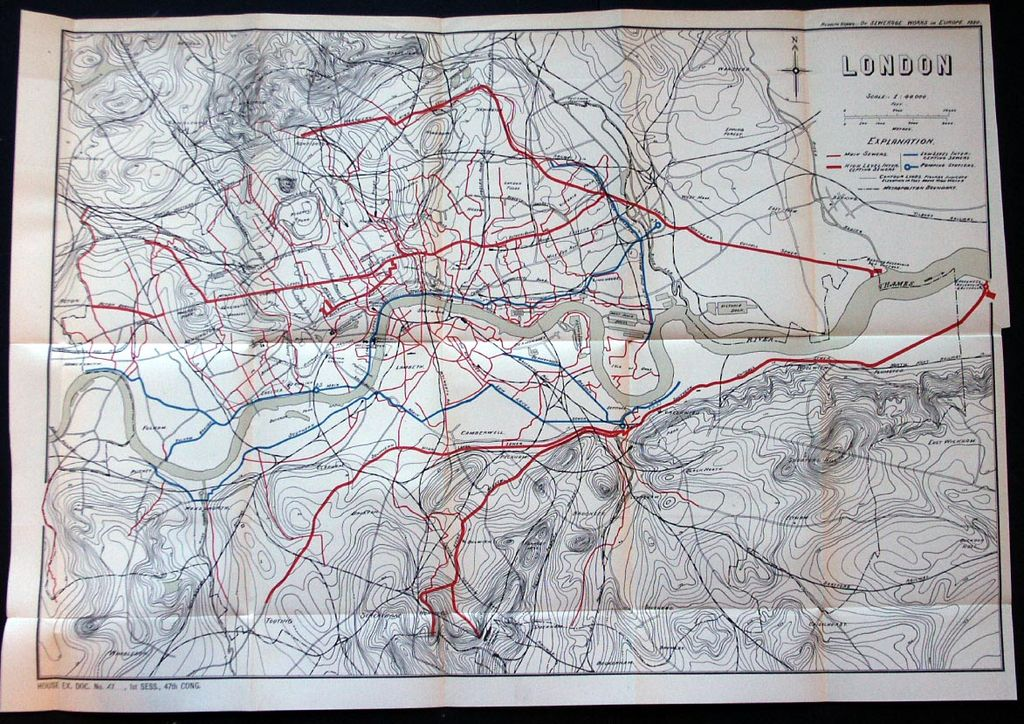
\includegraphics[width=1\textwidth]{2-cap1/complementos/mapas/1882-bazalgette-sistemadeesgotolondrino.jpg}{\par \footnotesize \textbf{Fonte:} \url{https://commons.wikimedia.org/wiki/File:Hering_lon-sewer-det02_1882.jpg}. \par}
\label{fig:esgotoslondres1882} 
\end{sidewaysfigure}

Entre uma epidemia e outra, um pesquisador assistente da \textit{Metropolitan Comission of Sewers}, \textit{Joseph William Bazalgette}, foi nomeado em 1856 diretor do órgão que veio a sucedê-la, o \textit{Metropolitan Board of Works}, e lá ficou até 1889; neste cargo, Bazalgette viveu em julho e agosto de 1858 -- como todos os londrinos -- o \textit{Grande Fedor}, causado pela exacerbação, pelo calor da época, do cheiro dos excrementos humanos não tratados e dos efluentes industriais que então eram lançados diretamente no Tâmisa. No mesmo ano, Bazalgette conseguiu aprovar junto ao Parlamento a construção, em Londres, de 132km de largas manilhas e canais em pedra para interceptar o afluxo de esgoto, e 1.800km de esgotamento de rua para captar os dejetos que, até então, fluiam livremente pelas ruas e vias públicas londrinas. Este fluxo de dejetos foi canalisado a jusante do Tâmisa, onde era despejado ainda sem tratamento. O plano de Bazalgette envolveu estações de bombeamento em \textit{Deptford Creek} e \textit{Crossness Point}, nos brejos de \textit{Erith}, todos no lado sul do Tâmisa; em \textit{Abbey Mills}, no vale do rio \textit{Lea}; e no aterro de \textit{Chelsea}, perto da ponte \textit{Grosvenor}, ao norte do Tâmisa \cite{bazalgette_london_1865, bazalgette_metropolitan_1865}. Embora Bazalgette fosse também adepto da teoria miasmática e pensasse, muito sinceramente, que a enorme obra sanitária que dirigiu serviria para acabar com os ``maus odores'' e, consequentemente, com as doenças epidêmicas, seus esforços tiveram sucesso, de fato, mas por um curioso efeito adverso: alargar a rede de esgotamento sanitário domiciliar e a drenagem pluvial significava conter, isolar e afastar do meio humano o bacilo do cólera, malgrado os miasmáticos duvidarem de sua existência.

\begin{figure}
\centering
\caption{Rambuteau e Haussmann, pioneiros do urbanismo e do planejamento urbano na França.}
\begin{footnotesize}
	\begin{subfigure}[b]{0.4\linewidth}
		\centering
		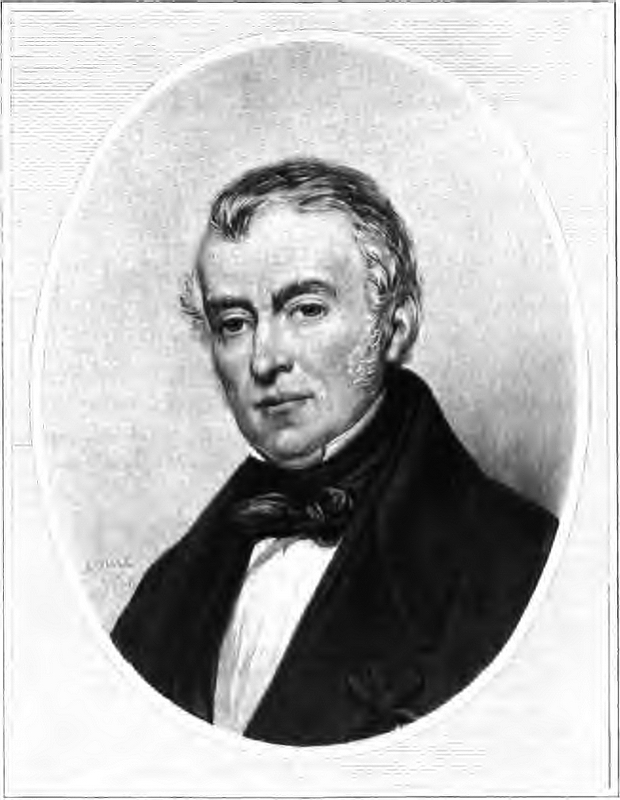
\includegraphics[width=1\textwidth]{2-cap1/complementos/fotos/Rambuteau.jpg} 
		\caption{Claude-Philibert Barthelot, conde de Rambuteau. \textbf{Fonte:} \url{https://commons.wikimedia.org/wiki/File:Le_comte_de_Rambuteau,d'après_Court,_1838_MMCR.jpg}.}
		\label{fig:rambuteau}
	\end{subfigure}	
	\
	\begin{subfigure}[b]{0.4\linewidth}
		\centering
		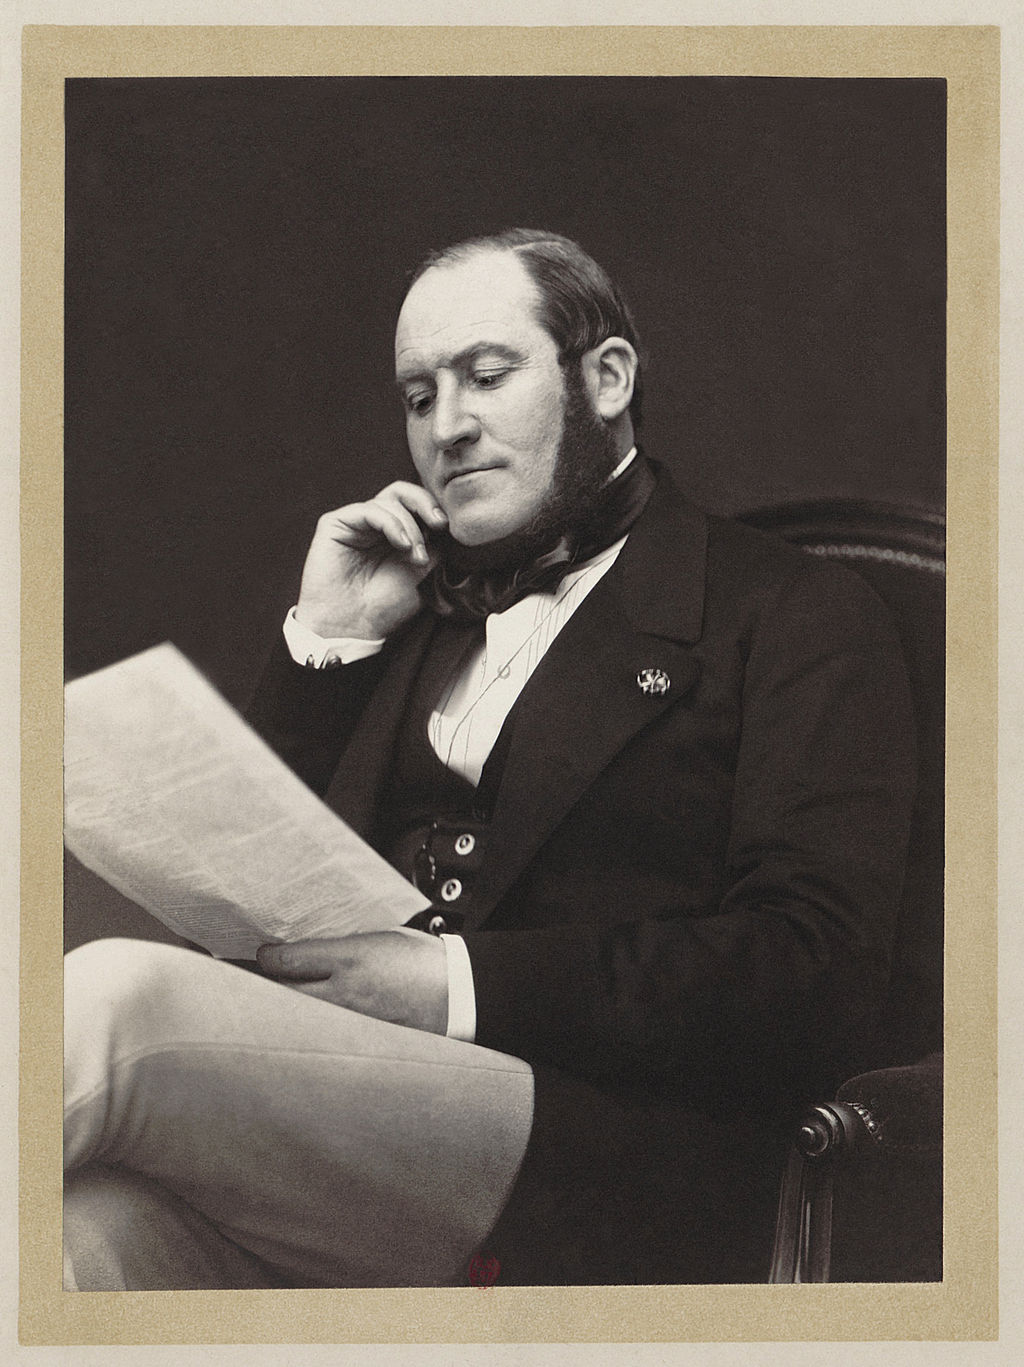
\includegraphics[width=1\textwidth]{2-cap1/complementos/fotos/haussmann.jpg}  
		\caption{Georges Eugène Haussmann. \textbf{Fonte:} \url{https://commons.wikimedia.org/wiki/File:Haussmann_BNF_Gallica.jpg}.}
		\label{fig:haussmann}
	\end{subfigure}	
\end{footnotesize}
\end{figure}

Vejamos agora a correlação entre teoria miasmática e obras públicas em \textit{Paris}. A ideia de realizar profundas reformas no centro de Paris era tão antigo e recorrente, sob diferentes formatos e nomes, que antecedeu ao \index{Georges-Eugène Haussmann}\index{Haussmann|seealso{Georges-Eugène Haussmann}}Haussmann prefeito, e que poderia, inclusive, ter sido feito inclusive sem ele. A cidade, quando de sua epidemia de cólera em 1832, havia crescido rumo aos \textit{faubourgs} em torno dos bulevares de Luís XIV, construídos em substituição às suas antigas muralhas; o centro mantinha as características medievais (principalmente as ruas estreitas e a malha viária irregular) e era dominado por uma encarniçada classe de proprietários, ciosa de seus direitos e pronta a defendê-los em qualquer instância onde se fizesse necessário \cite{faure_paris_2004}. Em 1833 \textit{Claude-Philibert Barthelot, conde de Rambuteau} foi posto à frente da prefeitura do Sena, onde permaneceu até 1848. Considerou ser seu dever ``dar aos parisienses água, ar e sombra'' \cite[p.~269]{rambuteau1905memoires}, comprimidos que eram pelas ruas estreitas e apertadas da cidade medieval; Rambuteau via-se no Hôtel de Ville como um ``comandante numa cidadela'' \cite[p.~269]{rambuteau1905memoires}, e assim tentou agir. A epidemia de cólera que assolou Paris em 1832 serviu a Rambuteau para dar início a um programa de melhoramentos urbanos iniciados com a abertura da \textit{Rue de Chanvreire} (atual \textit{Rue Rambuteau}), em 1834, com largura de 13 metros (incomum para os padrões da época), ligando o \textit{Marais} a \textit{Les Halles}; foi também aberta a \textit{Rue d'Arcole}, que atravessava a \textit{Île de la Cité} desde o arco da catedral de \textit{Notre-Dame} até o \textit{Hôtel de Ville} (ambos reformados, e o último ampliado, durante a gestão de Rambuteau); outras 112 ruas foram abertas. Seguiu-se a generalização da iluminação a gás em Paris, deixando Rambuteau ao sair de seu cargo 8.600 lampiões instalados; a rede de esgoto parisiense foi modernizada; novas pontes sobre o Sena foram construídas, sendo as mais famosas as de \textit{Bercy}, \textit{Saint-Pères} e Luís Felipe; a ilha de \textit{Louviers} foi anexada à margem direita do Sena por meio de um aterro. Rambuteau, ainda perseguindo seu programa de ``água, ar e sombra'', mandou plantar milhares de árvores e podar as já existentes; supervisionou a proliferação das ruas convexas, separadas das calçadas por sarjetas de escoamento, em substituição às antigas ruas côncavas em que as águas servidas acumulavam-se em poças; trouxe a Paris a pavimentação asfáltica, inicialmente ao redor do \textit{Palais-Royal}; ordenou a perfuração de poços em \textit{Grenele} e a instalação de duas mil fontes públicas com água encanada; a nota cômica deste processo de renovação urbana é o fato de os mictórios públicos instalados espaçadamente nos logradouros neste período terem sido apelidados de \textit{rambuteaux} em sua ``homenagem'' (\citeauthor{combeau_paris_2011}, \citeyear{combeau_paris_2011}, pp.~71-73; \citeauthor{rambuteau1905memoires}, \citeyear{rambuteau1905memoires}, pp.~325-399; \citeauthor{petti_eurfranba_2011}, \citeyear{petti_eurfranba_2011}, pp.~73-74). Em sua própria opinião, o conde de Rambuteau não pensa ter falhado em sua tarefa, pois teria feito o possível dentro das limitações legais e, no fim das contas, deixou a prefeitura do Sena sem dívidas \cite[p.~399]{rambuteau1905memoires}. 

O programa higienista concretizado primeiramente sob a gestão de Rambuteau foi retomado em escala monumental entre 1853 e 1870 por \index{Georges-Eugène Haussmann}\index{Haussmann|seealso{Georges-Eugène Haussmann}}\textit{Georges Eugène Haussmann} em seu mandato à frente da prefeitura do Sena. Recentes descobertas arquivísticas demonstram que a participação de \index{Georges-Eugène Haussmann}\index{Haussmann|seealso{Georges-Eugène Haussmann}}Haussmann na concepção geral das reformas no centro de Paris, ao contrário do que ele dá a entender em suas memórias (\citeauthor{haussmann1890memoires-1}, \citeyear{haussmann1890memoires-1}, \citeyear{haussmann1890memoires-2}, \citeyear{haussmann1890memoires-3}), foi menor do que se pensa: a \textit{Commission des embellissements de Paris}, nomeada diretamente por Napoleão III, composta por topógrafos, engenheiros e profissionais correlatos (como \textit{Théodore Jacoubet}, \textit{Hippolyte Meynadier} e os irmãos \textit{Louis} e \textit{Félix Lazaire}), reuniu-se pela primeira vez em 16 de agosto de 1853 e trabalhou até que seu diretor, \textit{Henri Siméon}, entregou ao imperador em 27 de dezembro de 1853 um plano bastante completo das modificações a serem feitas em Paris; muitas delas foram discutidas entre Napoleão III e a \textit{Comission} sem que \index{Georges-Eugène Haussmann}\index{Haussmann|seealso{Georges-Eugène Haussmann}}Haussmann sequer tomasse parte; foi o plano resultante dos trabalhos da \textit{Comission}, com algumas alterações, que \index{Georges-Eugène Haussmann}\index{Haussmann|seealso{Georges-Eugène Haussmann}}Haussmann implementou durante sua gestão à frente da prefeitura do Sena, depois de haver pedido -- e conseguido -- a extinção da comissão \cite{bourillon_changer_1999,casselle_embel_1997}\footnote{O artigo pioneiro de \citeonline{casselle_embel_1997}, quem primeiro divulgou a existência deste plano, chega a comparar, uma a uma, todas as obras propostas pela \textit{Comission} com aquelas realizadas por \index{Georges-Eugène Haussmann}\index{Haussmann|seealso{Georges-Eugène Haussmann}}Haussmann ou por seus sucessores. Observa, adicionalmente, que a cidade inteira foi coberta pelo projeto original (enquanto \index{Georges-Eugène Haussmann}\index{Haussmann|seealso{Georges-Eugène Haussmann}}Haussmann trabalhou principalmente na sua parte oeste), e que a malha viária dos antigos subúrbios anexados em 1860 estava, também, já desenhada no plano da \textit{Comission} de 1853, como a indicar um plano concebido de antemão.}. Quer como mentor intelectual, quer como gestor a mão-de-ferro de planos pré-concebidos, as obras regidas por \index{Georges-Eugène Haussmann}\index{Haussmann|seealso{Georges-Eugène Haussmann}}Haussmann, ao contrário daquelas regidas por Rambuteau, são muito maiores em escala e número, e muito mais conhecidas e comentadas \cite{bourillon_changer_1999, casselle_embel_1997, dansette_haussmann_1972, faure_paris_2004, hourticq_haussmann_1971, petti_eurfranba_2011, pinkney_ordevpar_1955, pinkney_paris_1957, vossen_villes_1947}, sendo desnecessário para o objeto desta pesquisa detalhá-las neste momento; cabe, muito mais, ressaltar que \index{Georges-Eugène Haussmann}\index{Haussmann|seealso{Georges-Eugène Haussmann}}Haussmann era outro adepto da teoria miasmática (\citeauthor{haussmann1890memoires-2}, \citeyear{haussmann1890memoires-2}, p.~318; \citeyear{haussmann1890memoires-3}, p.~421), e que a orientação geral das intervenções urbanas regidas por seus planos seguia, mesmo que não intencionalmente, o programa de Rambuteau e de outros predecessores (Chabrol, Berger, o ``plano dos artistas'', os largos \textit{boulevards} à moda de Luís XIV etc.). Num só e grande resumo:

\begin{citacao}
Mas, afinal, o que é haussmannização? Através dos escritos de \index{Georges-Eugène Haussmann}\index{Haussmann|seealso{Georges-Eugène Haussmann}}Haussmann, não se pode chegar a um conceito preciso, uma vez que ele não propõe uma doutrina ou uma teoria de melhorias urbanas.
[\dots] O próprio \index{Georges-Eugène Haussmann}\index{Haussmann|seealso{Georges-Eugène Haussmann}}Haussmann chama seu trabalho de regularização, que não pretende uma universalidade científica, não se baseia numa crítica social, nem propõe um modelo espacial.
[\dots] As intervenções haussmannianas mudam a maneira de pensar a cidade, tomando como principal elemento a rua e criando uma rede viária composta por um tecido arquitetônico que destrói bairros insalubres e vielas. Expulsam a população residente, melhoram a higiene e a circulação, mudam a imagem da área central, e a cidade prepara-se para um novo modo de vida. A rua do século XIX destrói e modifica a rua medieval. A caixa da rua aumenta, as fachadas são reconstruídas, os trechos irregulares são substituídos por outros com desenho regular, geométrico e reto. Diferentes dos bulevares de Luís XIV -- projetados no lugar das antigas muralhas, locais para o desfrute e o passeio --, os bulevares do século XIX, de \index{Georges-Eugène Haussmann}\index{Haussmann|seealso{Georges-Eugène Haussmann}}Haussmann, são artérias criadas para a circulação rápida, o tráfego pesado. O espaço haussmanniano é o espaço público -- a rua, o passeio, as praças --, o espaço da mobilidade. A originalidade desse projeto está no conceito de sistema de circulação e de respiração, que superpõe malhas hierarquizadas, pertencentes a uma rede em estrela. Esse desenho não resulta num espaço homogêneo, uma vez que se acentua a divisão social entre leste e oeste, entre periferia e centro, mas ainda não se adota a ideia de cidade por setores. A hierarquia do sistema de comunicações muda a ordem de valores.
[\dots] Na cidade haussmanniana, é introduzida uma nova forma de construção da paisagem urbana. As intervenções no núcleo central tratam o conjunto dos espaços heterogêneos como uma entidade única e o dotam de isotropia. Constrói-se uma imagem urbana mais coerente, com um tipo de arquitetura definida, em que o imóvel se integra no espaço público através de uma projetação regulamentada \cite[pp.~68,~77]{petti_eurfranba_2011}.
\end{citacao}

A saúde pública e o bem-estar dos cidadãos parisienses era o principal argumento para a instalação, reforma ou ampliação de infraestruturas sanitárias e equipamentos coletivos, mas não era possível esconder os profundos arranjos financeiros necessários a tais reformas: a oposição parlamentar a Napoleão III atacou \index{Georges-Eugène Haussmann}\index{Haussmann|seealso{Georges-Eugène Haussmann}}Haussmann incessantemente pela falta de transparência nos gastos, especialmente com o escândalo das transações escusas envolvendo o \textit{Crédit Foncier}, a \textit{Caisse des Travaux de Paris} e a firma \textit{Ardoin, Ricardo et Cie.} \cite{pinkney_paris_1957}. Houve desde o início das intervenções resistência encarniçada ao programa de reformas também entre proprietários, que julgavam indevidas as expropriações e as intervenções sobre suas propriedades \cite{paccoud_hauspropr_2012}. A força combinada destas pressões políticas levou Napoleão III a retirar o apoio a \index{Georges-Eugène Haussmann}\index{Haussmann|seealso{Georges-Eugène Haussmann}}Haussmann, que saiu da prefeitura do Sena em 1870. Não obstante, as reformas ditas ``haussmannianas'' (mais bem descritas como \textit{reformas do Segundo Império}), numa Paris cujo centro estava sendo progressivamente abandonado pelas classes abastadas e ocupado pelos trabalhadores e pelos miseráveis, cujos alugueis abasteciam os bolsos dos proprietários fundiários, teria beneficiado exatamente os mais abastados, já em vias de instalação nos \textit{faubourgs} e subúrbios parisienses, a obter vantagens na luta encarniçada pela retomada do centro de Paris \cite{faure_paris_2004}.

\begin{figure}[!htp]
\centering
\caption{Duas obras do período de Georges Eugène Haussmann à frente da prefeitura do Sena.}
\begin{subfigure}{0.9\textwidth}
\centering
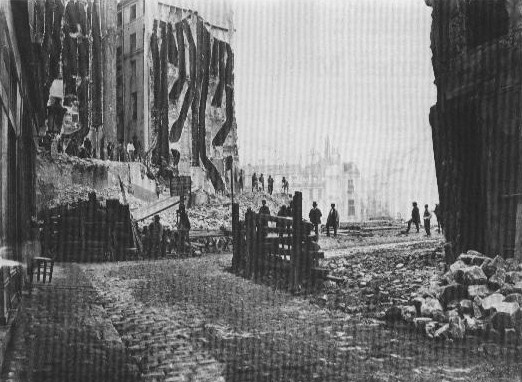
\includegraphics[width=1\textwidth]{2-cap1/complementos/fotos/Percement_avenue_de_lOpera.jpg}{\par \footnotesize Abertura da \textit{Avenue de l'Ópera}. \textbf{Fonte:} \url{https://commons.wikimedia.org/wiki/File:Percement_avenue_de_l'Opéra.jpg}.}
\label{fig:aberturaopera}
\end{subfigure}
\
\begin{subfigure}{0.9\textwidth}
\centering
\includegraphics[width=1\textwidth]{2-cap1/complementos/fotos/rivoli.jpg}{\par \footnotesize Construção noturna da \textit{Rue de Rivoli}\textbf{Fonte:} \url{https://commons.wikimedia.org/wiki/File:Travaux_nocturnes_des_constructions_de_la_rue_de_Rivoli,_éclairés_par_la_lumière_électrique.jpg}. }
\label{fig:obrasrivoli}
\end{subfigure}
\end{figure}

A análise de exemplos poderia incluir a construção em Viena (Áustria) da \textit{Ringstrasse} e seus prédios monumentais por ordem do imperador Francisco José I (1857-1913) \cite{abercrombie_vienna_1910,abercrombie_vienna_1911,aman_vienna_1911}; poderia incluir o ``embelezamento'' de Bruxelas (Bélgica) sob a regência do burgomestre \textit{Jules Anspach} e do rei \textit{Leopoldo II} (\textit{le roi bâtisseur}, ``o rei construtor''), em especial o tamponamento e canalização do Sena entre 1859 e 1873 \cite{abercrombie_brussels1_1912,abercrombie_brussels2_1912,abercrombie_brussels3_1913}; poderia avançar pela expansão de Barcelona de acordo com o plano pioneiro de \textit{Ildefonso Cerdà} (1860) \cite{aibarbijker_barcelona_1997,ciervo_cerda_1976,soriaypuig_cerda_1995,wynn_barcelona_1979}; poderia seguir pelo \textit{Risanamento} de Florença (1865-1895), Nápoles (1885-1904) e outras cidades italianas em seguida à \textit{Unificazione} \cite{biocca_naples_1992,parisi_napoli_2001,piccinato_igiene_1989,rossi_napoli_2011}\dots Há um longo fio condutor a ligar o higienismo dos primeiro e segundo terços do século XIX ao ``proto-urbanismo'' do último terço deste mesmo século e ao urbanismo do primeiro terço do seguinte -- se é que há, realmente, alguma solução de continuidade, salvo pela escala e escopo das intervenções propostas em ambos os casos. 

\begin{a3paisagem}
\begin{figure}[!htp]
\caption{Planta de situação da capital e da cidade residencial de Berlim e seus arredores -- plano de desenvolvimento dos arredores de Berlim (1856).}
\centering
\includegraphics[height=0.9\textheight]{2-cap1/complementos/mapas/1856_Bauplanungen.jpg}{\par \footnotesize \textbf{Fonte:} \url{https://commons.wikimedia.org/wiki/File:1856_Bauplanungen.jpg}.}
\label{fig:bauplannungen1856} 
\end{figure}
\end{a3paisagem}

\begin{a3paisagem}
\begin{figure}[!htp]
\caption{Plano para Berlim e arredores até Charlottenburg (1862), desenhado por Ferdinand Boehm.}
\centering
\includegraphics[height=0.9\textheight]{2-cap1/complementos/mapas/Boehm_Berlin_1862.jpg}{\par \footnotesize \textbf{Fonte:} \url{http://nbn-resolving.de/urn:nbn:de:kobv:109-opus-104224}. Os 14 departamentos do \textit{plano Hobrecht} estão rotulados como algarismos romanos. Os assentamentos programados estão indicados por letras maiúsculas e ruas por meio de algarismos arábicos, cada um dentro de um departamento de planejamento.}
\label{fig:berlin1862} 
\end{figure}
\end{a3paisagem}

\begin{a3paisagem}
\begin{figure}[!htp]
\caption{Plano de Giuseppe Poggi para Florença (1865).}
\centering
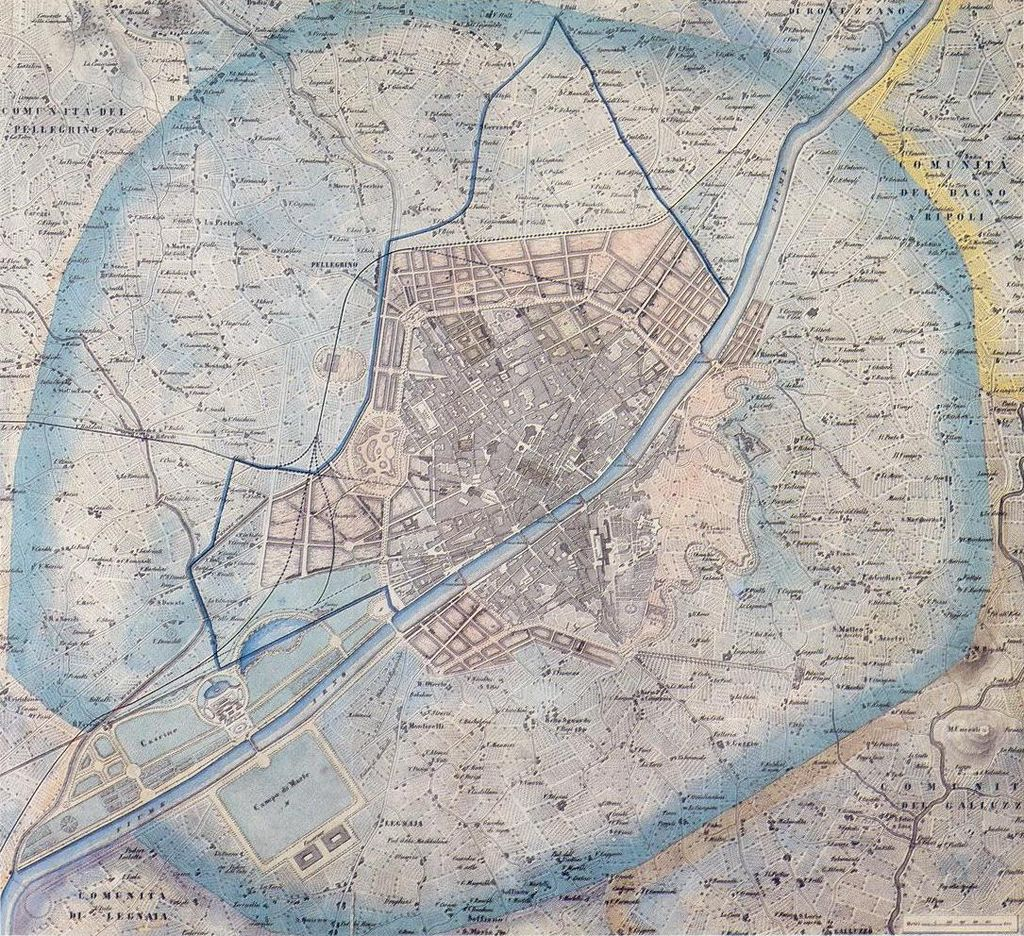
\includegraphics[height=0.9\textheight]{2-cap1/complementos/mapas/1865-planopoggi-florenca.jpg}{\par \footnotesize \textbf{Fonte:} \url{https://commons.wikimedia.org/wiki/File:Piano_Poggi_(Firenze,_1865)_-_1.JPG}.}
\label{fig:florenca1865} 
\end{figure}
\end{a3paisagem}

\begin{a3paisagem}
\begin{figure}[!htp]
\caption{Plano da cidade de Heilbronn, por Reinhardt Baumeister (1879).}
\centering
\includegraphics[height=0.9\textheight]{2-cap1/complementos/mapas/heilbronn.jpg}{\par \footnotesize \textbf{Fonte:} \url{https://commons.wikimedia.org/wiki/File:Stadtbauplan_Heilbronns_von_1879_auf_der_Grundlage_des_Generalbebauungsplanes_von_Reinhard_Baumeister.jpg}. }
\label{fig:heilbronn1879} 
\end{figure}
\end{a3paisagem}

Para os fins desta pesquisa, entretanto, os dois casos paradigmáticos apresentados já demonstram, sem necessidade de análise detalhada de outros exemplos, que o alvo preferencial das políticas do higienismo no século XIX foram os \textit{centros urbanos ditos ``degradados''} e as \textit{construções insalubres}. Ora, mas \textit{quem morava em tais construções e centros era exatamente quem não tinha condições de pagar para morar em imóveis em condições mais higiênicas}; ``higienizar'', ``embelezar'', fazer ``melhoramentos'' implicou, na maioria dos casos, em \textit{processos maciços de remoção dos trabalhadores e dos mais pobres dos bairros centrais}\footnote{No caso francês, \citeonline[p.~445]{faure_paris_2004} registra que ``dos 102 imóveis construidos nos anos 1860 pela companhia imobiliária dos irmãos Péreire, no atual bulevar Voltaire -- ou seja, num \textit{faubourg} do leste de Paris -- apenas 19\% dos apartamentos, dado o valor dos alugueis, parecem, a rigor, acessíveis a famílias operárias, a menos que se trate de cubículos nos sótãos''. Diz ainda que ``as operações de 1849-1853 tiveram como efeito desalojar 9.081 'trabalhadores' [\dots]: 2,1\% partiram para os \textit{banlieues}, e a imensa maioria dos outros se distribuiriam nos \textit{faubourgs}, uma reduzida minoria tendo permanecido nos bairros do centro, esperando, sem dúvida, que a continuação das obras não lhes desse caça'' (\Ibidem[p.~445]{faure_paris_2004}). No caso napolitano, tanto antes quanto depois do \textit{Risanamento} \citeonline{serao1906ventre} denunciou o caráter deletério das condições de vida dos trabalhadores mais pobres. No caso vienense, a \textit{Ringstrasse} acentuou a segregação socioespacial já existente, separando os burgueses da nova e resplandescente avenida, os operários dos subúrbios industriais como \textit{Ottakring} e uma pequena burguesia saudosa da antiga cidade \cite[p.~26]{maderthanermuser_vienna_2003}.}. O longo experimento higienista do século XIX interferiu também sobre a moradia, em especial sobre a moradia dos trabalhadores. A \textit{habitação operária} tornou-se, em paralelo à questão sanitária, pauta importante para os gestores públicos e os encontros internacionais de arquitetos e engenheiros: infiltou-se no Congresso Internacional de Higiene de 1878 em Paris \cite{congres_hygiene_1878}, fato repetido nos congressos internacionais de arquitetos de Londres (1908) e Viena (1910) \cite{QUINTOJR1990}, e mereceu um congresso internacional voltado apenas ao seu debate \cite{fleming_housing_1897}. Em nenhum deles, entretanto, chegou-se a qualquer solução definitiva quanto à questão, restringindo-se tais encontros ao relato das experiências locais em habitação operária e a soluções tópicas\footnote{Veja-se, como exemplo, o voto final da sessão plenária de 7 de agosto do Congresso Internacional de Higiene de 1878: depois de longos relatos e debates sobre a habitação dos operários em Paris, Londres, Bruxelas e outras metrópoles europeias, os presentes concordaram numa única recomendação: reforçar a legislação urbanística existente e transformar em exigência legal a instalação de água nas casas para operários \cite[p.~597]{congres_hygiene_1878}.}.

Tudo indica, até o momento, que os conflitos sociais são elemento essencial da produção, apropriação e uso dos territórios urbanos no período. Mas se há conflito social neste âmbito, seria a estética arquitetônica, ela própria, também produto dos conflitos sociais de seu tempo? Ou estaria imune a tal influência?

\subsubsection{As artes de morar: ecletismo e pré-modernismos, por dentro e por fora}\label{subsec:armor}

Entre os estilos arquitetônicos dezenovistas, o que mais interessa a esta pesquisa, pelo que se pôde encontrar nos documentos consultados, é como que um ``não-estilo'': o \textit{eclético}, resumidamente conceituado por um especialista como

\begin{citacao}
a cultura arquitetônica própria de uma classe burguesa que dava primazia ao conforto, amava o progresso (especialmente quando melhorava suas condições de vida), amava as novidades, mas rebaixava a produção artística e arquitetônica ao nível da moda e do gosto \cite[p.~13]{patetta_ecletismo_1987}.
\end{citacao}

A própria etimologia grega da palavra -- o adjetivo \textgreek{ἐκλεκτικός}, \textit{eklektikos}, ``escolhido entre os melhores'', por sua vez derivado de \textgreek{ἐκλεκτός}, \textit{eklektos}, ``escolhido, seleto'' -- indica uma de suas características principais: a escolha pelo arquiteto ou por seus clientes, na tradição arquitetônica passada, de elementos ora coerentes, ora díspares, que compusessem a obra de acordo com o gosto do freguês ou com a função a ser dada ao imóvel. Justo por isto, há enorme heterogeneidade estilística no campo eclético, sendo bastante difícil encontrar elementos comuns que não as justaposições e os revivalismos. 

Como movimento artístico, o ecletismo ocorre na arquitetura e na arte do século XIX. As primeiras vanguardas desse movimento datam da terceira década do século XIX com a afirmação de pulsões neo-góticas em áreas francófonas e neo-renascentistas em Florença. Por volta de 1840, na França, em reação à hegemonia do estilo greco-romano, os arquitetos começam a propor a retomada de outros modelos históricos como, por exemplo, o gótico e o românico. O principal teórico do ecletismo arquitetônico é o francês \textit{César Denis Daly} (1811-1893) que o entende como ``o uso livre do passado''. Não se trata de uma atitude de simples copista, mas da habilidade de combinar as características superiores desses estilos em construções que satisfaçam a demandas da época por todo tipo de edificação. Na segunda metade do século XIX, o ecletismo tem forte presença na Europa. O estilo \textit{Segundo Império} ou \textit{Napoleão III} é caracterizado pela realização de importantes edifícios ecléticos, como o Teatro Ópera de Paris, projetado por \textit{Charles Garnier} (1825-1898).

\begin{figure}[!htp]
\centering
\caption{\textit{Hôtel privé} de primeira classe no estilo Segundo Império/Napoleão III.}
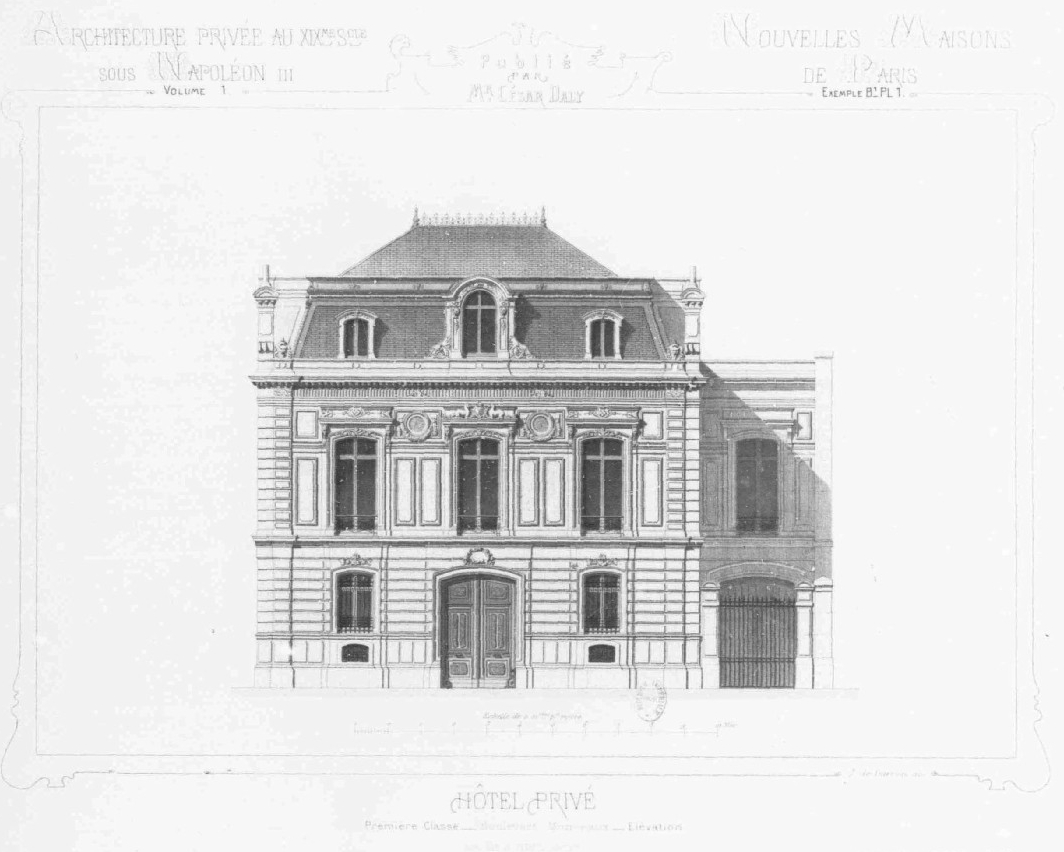
\includegraphics[width=1\textwidth]{2-cap1/complementos/fotos/daly01-0.JPEG}{\par \footnotesize \textbf{Fonte:} \textbf{L’architecture privée au XIXe siècle, sous Napoléon III:} nouvelles maisons de paris et des environs, de César Denis \citeonline{daly_architecture1_1864}. \par}
\label{fig:hotelprimclas} 
\end{figure}

\begin{figure}[!htp]
\centering
\caption{\textit{Hôtel privé} de segunda classe no estilo Segundo Império/Napoleão III.} 
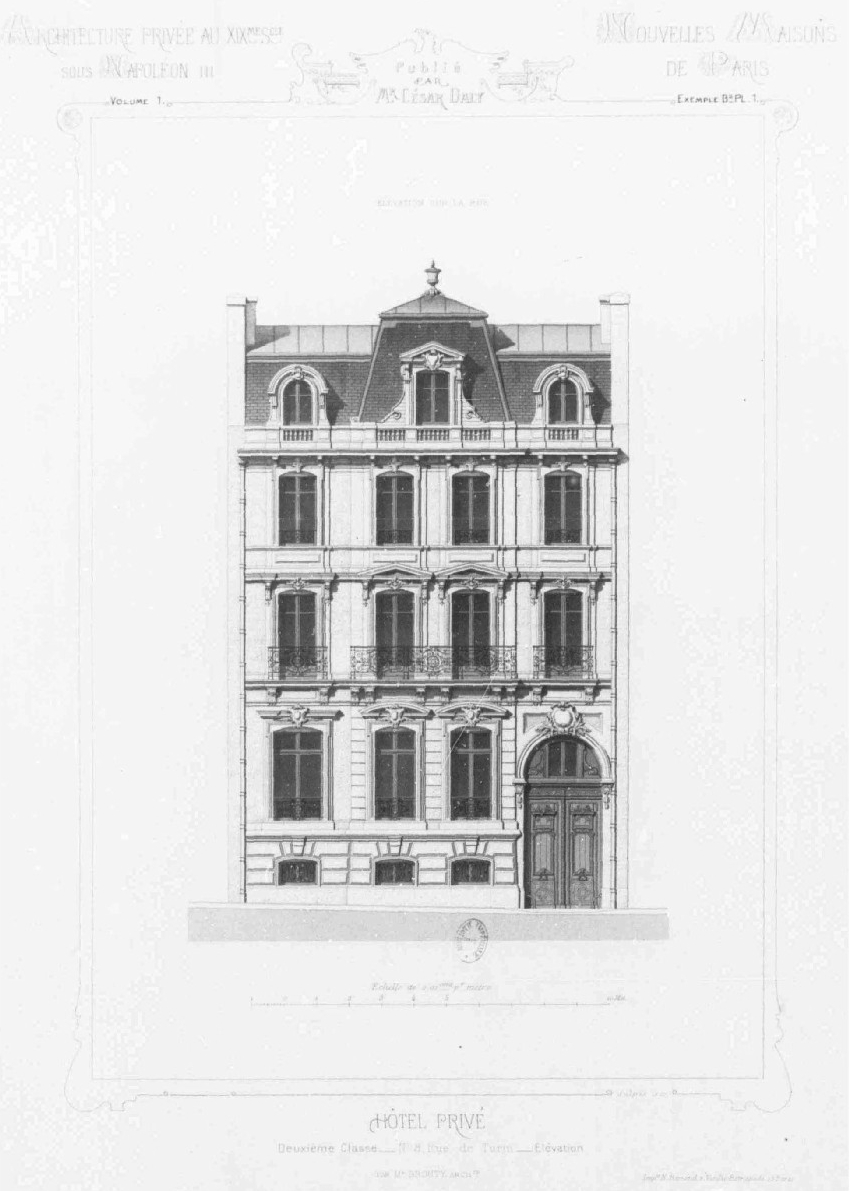
\includegraphics[width=1\textwidth]{2-cap1/complementos/fotos/daly01-1.JPEG}{\par \footnotesize \textbf{Fonte:} \textbf{L’architecture privée au XIXe siècle, sous Napoléon III:} nouvelles maisons de paris et des environs, de César Denis \citeonline{daly_architecture3_1864}. \par}
\label{fig:hotelsegclas} 
\end{figure}

\begin{figure}[!htp]
\centering
\caption{\textit{Villa suburbaine} de primeira classe no estilo Segundo Império/Napoleão III.}
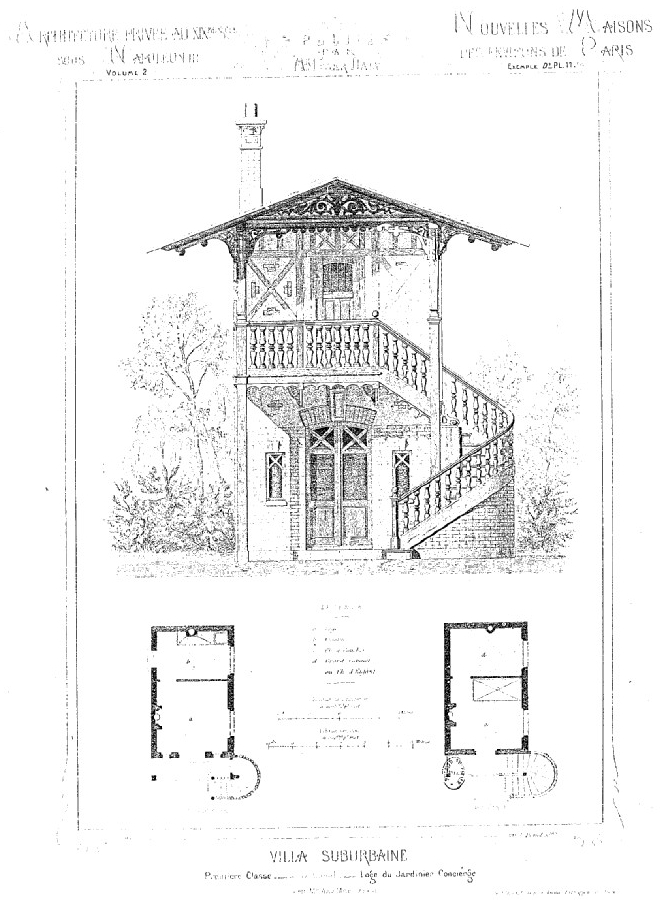
\includegraphics[width=1\textwidth]{2-cap1/complementos/fotos/daly03-4.JPEG}{\par \footnotesize \textbf{Fonte:} \textbf{L’architecture privée au XIXe siècle, sous Napoléon III:} nouvelles maisons de paris et des environs, de César Denis \citeonline{daly_architecture3_1864}. \par}
\label{fig:villaprimclas} 
\end{figure}

\begin{figure}[!htp]
\centering
\caption{\textit{Villas suburbaines} de segunda classe no estilo Segundo Império/Napoleão III.}
\begin{subfigure}[b]{0.8\linewidth}
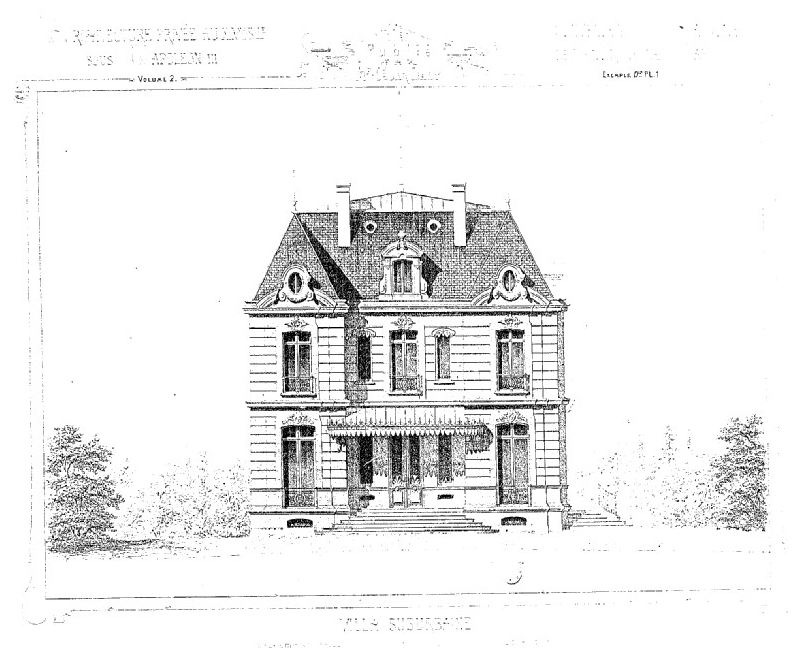
\includegraphics[width=0.9\textwidth]{2-cap1/complementos/fotos/daly03-5.JPEG}
\caption{\textbf{Fonte:} L’architecture privée au XIXe siècle, sous Napoléon III: nouvelles maisons de paris et des environs, de César Denis \citeonline{daly_architecture3_1864}.}
\label{fig:villasegclas1}
\end{subfigure}
\
\begin{subfigure}[b]{0.8\linewidth}
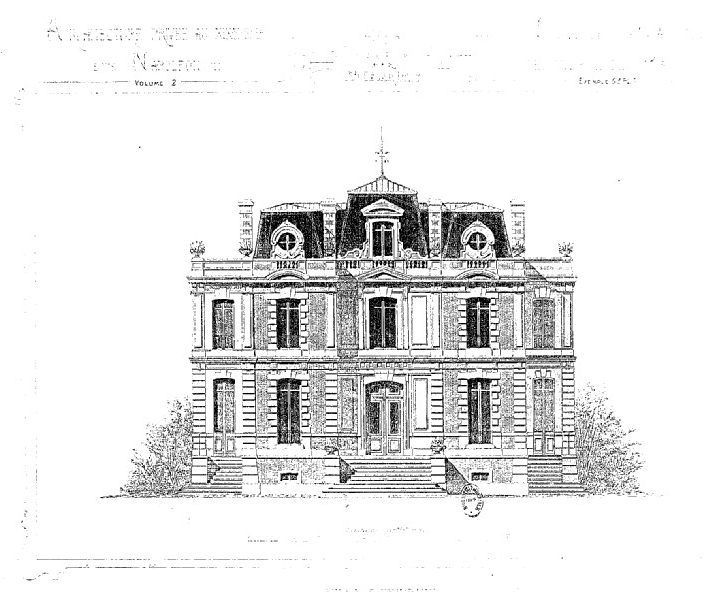
\includegraphics[width=0.9\textwidth]{2-cap1/complementos/fotos/daly03-6.JPEG}
\caption{\textbf{Fonte:} \textbf{L’architecture privée au XIXe siècle, sous Napoléon III:} nouvelles maisons de paris et des environs, de César Denis \citeonline{daly_architecture3_1864}.}
\label{fig:villasegclas2}
\end{subfigure}
\end{figure}

\begin{figure}[!htp]
\centering
\caption{\textit{Villa suburbaine} de terceira classe no estilo Segundo Império/Napoleão III.}
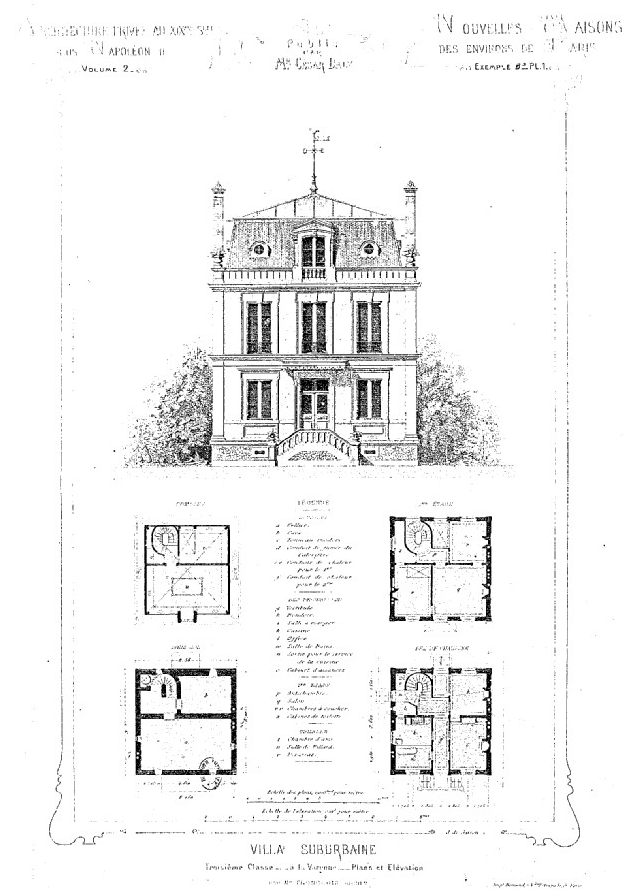
\includegraphics[width=1\textwidth]{2-cap1/complementos/fotos/daly03-8.JPEG}{\par \footnotesize \textbf{Fonte:} \textbf{L’architecture privée au XIXe siècle, sous Napoléon III:} nouvelles maisons de paris et des environs, de César Denis \citeonline{daly_architecture3_1864}. \par}
\label{fig:villaterclas} 
\end{figure}

As diferentes linguagens artísticas foram reelaboradas a critério do arquiteto seguindo a sua inspiração pessoal. No princípio a tendência eclética se impôs especialmente na realização de estruturas para festas e grandes eventos; sucessivamente, começou a ser apreciada também para mobiliar casas e jardins, nos quais, frequentemente e de forma totalmente acrítica, misturavam-se tempos gregos, vasos árabes e pavilhões indianos. Na época afirmou-se o costume de mobiliar cada sala das residências mais luxuosas segundo um estilo diferente. Assim, marceneiros e ebanistas, por exemplo, tiveram que aprender a lidar com formas bastante diferentes entre si. 

Mas foi o modernismo industrial do século XIX que serviu como trampolim para o sucesso do estilo eclético. Em 1851, pela primeira vez, na \textit{Great Exhibition} em Londres foram realizados pavilhões onde os mercadores das principais nações do mundo foram chamados para expor suas próprias obras. Percebeu-se que as empresas presentes exibiam para a atenção do publico obras que mostravam a história recente ou antiga da própria nação. Houve euforia em expor todas as obras antigas remodeladas, havendo-se, inicialmente, um certo grau de dependência relativamente aos modelos originais, quase como se fosse uma cópia, uma reprodução. A fantasia de cada artista, artesão, arquiteto, ourives, etc. não demorou para se afirmar, levando os artistas a formular obras personalizadas que ``condensavam'' vários séculos de história. Era isso o que os clientes queriam, curiosos por artes distantes e citações culturais magníficas mostrando que aquela geração iria reviver uma era áurea. Todas as grande técnicas do passado reviviam numa miríade de moveis, cerâmicas e
objetos do Ecletismo.

Grosso modo, as obras arquitetônicas em estilo eclético podem ser classificadas em três categorias principais, cujas características são assim definidas:

\begin{itemize}
\item A \textit{composição estilística}: caracteriza-se por um \textit{maior rigor filológico} e pela \textit{imitação precisa e coerente de um único e preciso estilo arquitetônico}. Os exemplos mais destacados são o \textit{neogrego}, o \textit{neo-egípcio} e o \textit{neogótico}.
\item O \textit{historicismo tipológico}: caracteriza-se por uma \textit{relação apriorística de cunho analógico entre estilo e função} através de valores associativos, não raro arbitrários. A arquitetura medieval, por exemplo, forneceu aos arquitetos os traços místicos e a religiosidade para as novas igrejas; na arquitetura renascentista foram encontradas as características áulicas elegantes para os edifícios públicos; na arquitetura barroca, ou nos estilos orientais, a festividade exigida pelos equipamentos; no classicismo pesado do coríntio romano, o caráter apropriado aos solenes edificios parlamentares, aos museus e aos ministérios.
\item Os \textit{pastiches compositivos}: caracterizam-se pela \textit{fusão de elementos arquitetônicos de estilos distintos, historicamente inadmissíveis}, sob cujos elementos díspares, não raro beirando o mau gosto, mascaravam-se muitas vezes soluções estruturais inovadoras \cite[p.~14-15]{patetta_ecletismo_1987}.
\end{itemize}

Quer seja ele o estilo ostentatório dos \textit{nouveaux riches} desprovidos da bagagem cultural do \textit{Ancièn Régime} e dispostos a demarcar seu espaço social por meio da sobreposição, às vezes sem nexo, das novas modas da Escola de Belas-Artes de Paris \cite[pp.~315-319]{guerrand_espacos_2009}, quer seja um estilo arquitetônico com méritos e conquistas próprios em processo de redescoberta desde pelo menos a metade dos anos 1970, a partir da crítica ao ideário arquitetônico do Modernismo que o sucedeu e criticou duramente \cite{almeida_victoria_1997, almeida_vitrinescomercio_2014, patetta_ecletismo_1987, puppi_hisnamod_1998}, interessa a esta pesquisa o fato de o ecletismo ser o estilo arquitetônico mais encontrado no distrito soteropolitano estudado, especialmente nas modalidades de \textit{historicismo tipológico} e \textit{pastiche compositivo}, com maior frequência esta última.

A América Latina foi terreno fértil para as experimentações arquitetônicas, especialmente as ecléticas, e isto por questões muito particulares. No final do século XIX, findos os processos independentistas, consolidadas as fronteiras nacionais e assentados os blocos hegemônicos na política após um século pontilhado por guerras, \textit{pronunciamientos} e rebeliões, as classes dominantes nos países latinoamericanos viram na arquitetura um meio de reafirmar sua identidade nacional. Curiosa e paradoxalmente, entretanto, tal como em outros campos da cultura, esta reafirmação se deu por meio de símbolos e elementos tomados de empréstimo por estas mesmas classes dominantes às edificações da aristocracia, dos banqueiros, dos grandes comerciantes e industriais da Europa \cite[pp.~403-406]{gutierrez_arquibero_1983}. Conquanto haja leitura destes empréstimos no sentido de criar uma clivagem entre colonizados e colonizadores, em que os primeiros -- como um todo, sem qualquer clivagem, estruturação, estratificação ou hierarquização social internas a si próprios -- encontrar-se-iam sempre no encalço destes últimos por quaisquer razões \cite{bhabha_local_1998,memmi_coloniza_1967}, na perspectiva adotada por esta pesquisa parece mais plausível radicar estes empréstimos nos deslocamentos miméticos de ideias e práticas devido à \textit{inserção subordinada destas classes dominantes no capitalismo internacional e no colonialismo} \cite{schwarz_ideias_1973}. As duas correntes, entretanto, concordam em que o deslocamento de ideias, símbolos e signos de seu contexto original produz efeitos bastante diversos no novo contexto em que se inserem, e que são eles, e não aqueles produzidos em seu ambiente de origem, que devem ser estudados. Esta ``chave de leitura'' será importante para a análise da urbanização brasileira na Primeira República, mais adiante.

E aqui, nesta etapa pré-modernista do pensamento e da prática acerca das cidades, se encerram as condicionantes sincrônicas internacionais relevantes para a presente pesquisa. As defasagens entre a produção e circulação de ideias nos meios profissonais levam a que as primeiras influências da arquitetura e do urbanismo europeus de vanguarda surgidas entre a última década do século XIX e as duas primeiras décadas do século XX, em seu pensamento ou realizações, só se façam sentir sobre o pensamento e a prática da arquitetura e do urbanismo em Salvador nos trabalhos da Semana de Urbanismo de 1935, que extrapolam o limite temporal escolhido\footnote{É certo, por exemplo, que Theodoro Sampaio mencionou explicitamente a influência sobre ele exercida pelas cidades-jardim \cite{costa1996theodoro}, e que já em 1913 estas mesmas cidades-jardins eram debatidas na imprensa baiana como contraponto ao desleixo da administração pública com o problema das moradias populares \cite{flexor_salvadorverde_2000}; apesar disto, nem o projeto da Cidade da Luz foi adiante (sua implementação em 1937 se deu vinte e oito anos depois da apresentação do projeto original de Theodoro Sampaio), nem os debates na imprensa avançaram além do confronto de ideias.}.
\section{A inserção brasileira no contexto internacional}\label{sec:insbrascontint}

É tempo, agora, de entender a inserção brasileira num contexto internacional de imperialismo, guerras, trustes e carteis. Nesta escala, já é possível analisar mais cerradamente a formação social e analisar, ainda que superficialmente, sua estrutura de classes, para, posteriormente, verificar a inserção da sociedade soteropolitana neste quadro.

A narrativa nesta seção parecerá repetitiva. Primeiro, uma visão geral da política brasileira durante a Primeira República; depois, uma caracterização dos investimentos internacionais por meio de capitais de diversas origens; em terceiro lugar, uma análise da sociedade brasileira em suas classes sociais constitutivas; por último, uma breve apresentação do desenvolvimento urbano brasileiro. Sujeitos se apresentarão repetidas vezes; relações entre classes serão repisadas; forças políticas e econômicas se reiterarão; fatos e datas emergirão redobradamente. Trata-se de exigência do \textit{método}: os mesmos fatos, os mesmos sujeitos e as mesmas forças serão vistos por diferentes pontos de vista, em diferentes situações, em meio a diferentes dinâmicas e escalas geográficas, para que a trama de suas relações seja analisada nos aspectos de interesse à pesquisa ora exposta. 

Tanto mais necessárias se fazem tais repetições e insistências quando a vasta maioria da literatura política, econômica e sociológica clássica no Brasil apresenta os longos quarenta anos da Primeira República como desprovidos de qualquer conteúdo de relevo para a historiografia brasileira senão as \textit{fraudes eleitorais}, a política dos Estados (ou ``política dos governadores'', ou ``política do café-com-leite''), o coronelismo em sua forma clássica, as crises econômicas e os \textit{funding loans} escorchantes etc.; a Primeira República teria sido como que um longo pesadelo, uma revolução burguesa incompleta, uma continuação republicana da hegemonia das ``oligarquias agrárias'' vigente desde o Império --- teria sido tudo, menos um período com características e legitimidade histórica próprias. Não cabe aqui fazer a crítica completa e adequada a tais concepções, pois o espaço deve ser aproveitado para uma apresentação sucinta dos conflitos sociais criadores das tendências políticas, econômicas e sociais interferentes na produção, apropriação e uso do espaço urbano de Brotas. Cabe, não obstante, registrar a divergência com tais concepções e discorrer de modo mais positivo daqui por diante, concentrando a exposição naquilo que de fato interessa à pesquisa cujos resultados aqui se expõem.

\subsection{Da República da Espada (1889-1894) à República do Café-com-Leite (1894-1930)}\label{subsec:espadaleite}

A proclamação da república no Brasil (1889) resulta não apenas das questões \textit{religiosa}\footnote{Costuma-se dar este nome a uma série de conflitos ocorridos entre 1873 e 1876 entre o clero e a maçonaria, de um lado, e entre o clero e a instituição regalista do \textit{padroado}, de outro; ambos podem ser enquadrados na \textit{reação ultramontana católica} iniciada no papado de Gregório XVI (1831-1846) e continuada no papado de Pio IX (1846-1878), especialmente por meio da encílica \textit{Quanta Cura} e seu infame anexo \textit{Sílabo dos Erros} (1864) e das posturas mais duras do Concílio Vaticano I (1869-1870), como resposta às revoluções liberais e ao secularismo. O conflito do clero com a maçonaria já se antecipava enquanto ordem papal em \textit{Quanta Cura} e no \textit{Sílabo dos Erros}, ambos contrários à liberdade de consciência e ao primado da razão; restou que Vital de Oliveira, bispo de Olinda, e Macedo Costa, bispo do Pará, acendessem o pavio aplicando tais doutrinas a seu pastorado, proibindo maçons em irmandades católicas, punindo padres maçons e engajando-se em polêmica impressa contra a maçonaria. O caso chegou até à Coroa, pois o regalismo instituído pelo padroado facultava ao imperador brasileiro interferir em assuntos clericais -- na prática, a igreja era quase totalmente submissa à Coroa, fato condenado tanto em \textit{Quanta Cura} quanto no \textit{Sílabo dos Erros}. Com a subsequente prisão dos bispos por desobedecerem à ordem imperial de suspender as sanções religiosas que haviam imposto aos maçons, a questão tomou vulto, transformou-se em transtorno diplomático com o Vaticano, resolvido com a absolvição imperial dos bispos em 1876, passando assim a Pedro II a imagem de ``submisso ao Papa'' tão fortemente aproveitada pela campanha republicana então nascente.}, \textit{militar}\footnote{Entre 1884 e 1887, uma série de incidentes envolvendo o tenente-coronel Antonio de Sena Madureira e o coronel Ernesto Augusto da Cunha Matos em questões que iam desde protestos quanto à contribuição obrigatória para o montepio militar ou o afastamento de oficiais acusados de corrupção geraram intensa polêmica impressa, resultando na proibição, por parte do Ministério da Guerra, de qualquer manifestação de militares através da imprensa. A mordaça gerou insatisfação na caserna, especialmente na Escola Militar da Praia Vermelha, onde já floresciam a filosofia positivista e o republicanismo.} ou mesmo da questão \textit{sucessória}\footnote{Uma vez que Pedro II teve apenas filhas como herdeiras e a constituição brasileira de 1824 instituíra a sucessão semi-agnática, que não exclui herdeiras do processo sucessório, Isabel era a herdeira do trono brasileiro; por ser casada com Luís Filipe Maria Fernando Gastão, conde d'Eu, tido como largamente impopular em razão de sua nacionalidade francesa, sua futura ascensão ao trono criou entre as classes populares, a classe média, os militares e outros a má expectativa de serem governados por um estrangeiro.}; por importantes que sejam estas questões como expressão das contradições e conflitos sociais do último período do Império, os problemas sociais e políticos que levaram à derrocada do regime imperial foram, fundamentalmente, aqueles decorrentes do \textit{escravismo} que sustentava o regime; a \index{abolição da escravidão}\textit{abolição da escravidão} foi o corolário do esgarçamento do pacto político que sustentou o regime dos Orleans e Bragança, e depois dela mesmo os aristocratas hegemônicos e frequentadores da corte sabiam que a monarquia tinha seus dias contados. 

Foi, na verdade, nos anos 1860 que começaram a se acumular fatores contrários à sustentação do regime escravista: a crise econômica dos anos 1860, causada pelo \textit{declínio nos preços do café} (principal pauta de exportação brasileira na época); a \textit{crise financeira de 1864}; a \textit{vitória dos Estados antiescravistas na Guerra de Secessão estadunidense}, com o consequente debilitamento dos Estados escravocratas (Brasil e Cuba) perante a opinião pública internacional; a \textit{Guerra do Paraguai}, onde massas de recém-libertos incorporadas à tropa foram tomadas pelas ideias de liberdade e insuflaram-nas entre a oficialidade; o \textit{declínio da população escravizada} e as \textit{migrações internas de escravos}, especialmente do Norte-Nordeste, para as regiões cafeeiras; tudo isto, enfim, resultou não apenas numa cúpula ministerial favorável à abolição, mas também ao florescimento de uma opinião pública também abolicionista, e ao surgimento das primeiras associações dedicadas à propaganda anti-escravista e à coleta de donativos para compra de alforrias \cite[p.~141-143]{gorender_escrareab_1990}. É o momento em que a rebelião negra contra a escravidão --- afogada pela maré montante da repressão que, como consequência da malograda \textit{Revolta dos Malês} e do terror que ela imprimiu sobre a aristocracia brasileira como um todo, desde o segundo terço do século XIX foi voltada contra os africanos escravizados --- assume novas formas e se intensifica; é de igual modo momento do dealbar, na cena política e social, de uma ``classe média'' urbana -- as aspas serão explicadas na \autoref{subsubsec:clamed} (p. \pageref{subsubsec:clamed}) -- patrocinadora de um \textit{movimento abolicionista} radicalizado, promotor não só da cotização para alforrias, mas igualmente de fugas individuais e coletivas de pessoas escravizadas \cite[p.~267-336]{saes_estadoburgues_1985}. Entender os dois processos separadamente implica numa separação injustificada entre entre uma esfera econômica e uma esfera política que só se podem compreender juntas. E muitas das contradições e conflitos sociais da Primeira República eram perceptíveis já aqui, nos últimos anos do Império.

É possível estabelecer, seguindo os passos de Edgar \citeauthoronline{carone_evolucao_1977}, uma periodização da fase civil da Primeira República: o \textit{fastígio do regime}, composto pelos mandatos presidenciais de Prudente de Moraes, Campos Sales, Rodrigues Alves e Afonso Pena num período que vai de 1890 a 1910; um período de \textit{abalos no regime}, composto pelos mandatos presidenciais de Hermes da Fonseca e Wenceslau Braz no período entre 1910 e 1918; e um último período marcado por fortes \textit{contestações ao regime}, composto pelos mandatos de Epitácio Pessoa, Artur Bernardes e Washington Luiz, iniciado em 1918 e encerrado com o advento da revolução de 1930, encerradora da Primeira República e inauguradora da era Vargas \cite{carone_evolucao_1977}. 

O período imediatamente posterior à proclamação da república no Brasil, conhecido como \textit{república da espada}, foi na verdade a primeira \textit{ditadura militar} republicana, convulsionada por agitações políticas de todos os tipos. Em disputa, não somente projetos políticos, mas o poder, e, em última instância, mesmo o regime. A crônica da época diz que o golpe militar responsável pela proclamação da república foi articulado por um grupo de jovens oficiais sem muita inserção entre a base da tropa e sem maior articulação com o oficialato superior, convocado à última hora para a ação \cite[p.~16]{cardoso_govmil_1977}; diz-se inclusive, como Aristides Lobo, que o povo assistiu ``bestializado'' a tudo aquilo, e que para o grosso da população brasileira, eminentemente rural e alijada dos processos políticos, ``a mudança do regime político a afetara tanto quanto a morte de um gato na China'' \cite[p.~43]{basbaum_histsinc_1967}. Frágil como fosse, a proclamação da república abriu uma década de rearranjo das bases e das forças políticas hegemônicas do país -- conquanto pouco alterasse sua estrutura social e econômica.

Os governos de \textit{Deodoro da Fonseca} e \textit{Floriano Peixoto} foram verdadeiras ditaduras militares, conhecidos para a História como \textit{República da Espada}. Deodoro governou pouco; Floriano pensava em construir um governo estável, acima das disputas locais, estaduais e regionais, cooptando quadros nas escolas civis e militares. Teria tudo para ser ferrenho adversário dos latifundiários, mas rapidamente surgiu uma aliança entre Floriano e os cafeicultores organizados no Partido Republicano Progressista (PRP), pois ambas as partes percebiam os riscos que corria a jovem república e viam-se reciprocamente como garantidores do novo regime: os latifundiários viam em Floriano a única possibilidade de garantir a sobrevivência do regime contra as forças centrífugas já então em pleno curso\footnote{Algumas destas forças centrífugas serão vistas adiante, na \autoref{subsec:clapolprire} (p. \pageref{subsec:clapolprire}); outras, como os \textit{monarquistas}, eram muito mais um espantalho a agitar nas peças de propaganda que uma ameaça real, tanto assim que deixaram de ser uma força política relevante já na década de 1910, tendo seu último estertor na tentativa gorada de tomar o poder em 1902 \cite{CARONE1970inst,janotti_subversivos_1986}.}, e Floriano via nos cafeicultores paulistas uma base de sustentação sobre a qual estruturar o projeto de um Estado forte. Não que se gostassem: \textit{aturavam-se} apenas, cada parte querendo avançar seus projetos políticos às custas da outra, como o episódio da passagem do poder de Floriano a \textit{Prudente de Morais} bem o exemplifica\footnote{``No dia 15 de novembro Prudente, trajado de acordo com o protocolo, aguardou, no hotel, que o viessem buscar. Só apareceu André Cavalcanti, convidado para Chefe de Polícia do seu Governo. Esperaram. Quando se convenceu de que não vinha ninguém, pediu ao amigo que se desse ao incômodo de ir ao Largo do Machado buscar condução. Veio o fiacre que ele conseguiu, um calhambeque em péssimo estado, o cocheiro mal enjambrado, e duas pilecas maltratadas. Foi nesse veículo sem pompa que o novo Presidente se transportou para o velho Palácio do Conde dos Arcos, onde prestou o compromisso legal. Acabada a cerimônia, o representante da Inglaterra, sabendo que o Presidente da República estava sem condução, ofereceu a sua esplêndida carruagem. Nela, Prudente se transportou para a sede do Governo. [\dots] O Palácio havia sido abanbdonado e entregue à discrição do público. O Itamarati recebeu o Presidente de portas abertas e salões vazios. Não apresentava o aspecto de uma casa de governo. Nâo havia uma mesa de trabalho, uma estante de livros, a menor demonstração de vida burocrática. [\dots] Seguido de poucas pessoas, esguio e solene, \textit{um doloroso sorriso} em meio àquele cenário, Prudente atravessa as dependências descuidadas. Na grande sala dos fundos, dando para o parque, jazia sobre o assoalho de custoso mosaico de madeira um caixão aberto, contendo jornais, papeis rasgados, garrafas vazias de cerveja e a palha que as envolvera. Os estofos de alguns móveis foram rasgados a pontaços de baionetas. Era inacreditável! Só então apareceu alguém do mundo oficial: era o Sr. Cassiano do Nascimento, ministro de quase todas as pastas do Governo Floriano. Fez um pequeno discurso dizendo que, em nome do Vice-Presidente fazia a transmissão do Governo. Depois disso, em consequência de uma pergunta de Prudente, o grupo dirigido por aquele ministro se encaminhou para ume pequena sala à esquerda que servia para o despacho presidencial. Então o Sr. Cassiano despediu-se e se retirou. Prudente instalava-se na Presidência da República do modo mais informal'' \cite[pp.~239-241]{silva_republica_1972}.}.

Em defesa da república, surgiram durante o governo Floriano Peixoto os ``jacobinos'' de 1893-1897, agrupados em torno de jornais como \textit{O Jacobino} e \textit{O Nacional}: gente como Júlio de Castilhos, Francisco Glicério, Deocleciano Martyr, Aníbal Mascarenhas e outros. Agitadores políticos profissionais, autoritários, anticlericais, defensores de medidas nacionalistas (tarifas de proteção à indústria e nacionalização do solo) e protetivas dos trabalhadores (como a jornada de oito horas e a regulamentação dos alugueis para operários), americanófilos e antilusitanos, atuavam ameaçando de morte os inimigos, intimidando-os com a publicação de seus nomes na sua imprensa (de longe a mais radical do período), provocando confrontos de rua, agitando o povo para depredações, insuflando ataques a portugueses (que tratavam, sem mais, como monarquistas) etc. \cite{queiroz_radicais_1986}\dots Tinham como base social principal o pequeno funcionalismo público das cidades e os militares de baixa e média patente. Com a perseguição aos suspeitos de envolvimento no atentado contra o presidente Prudente de Morais (05 nov. 1897), o movimento perdeu força e terminou dissolvendo-se em poucos anos.

Prudente de Morais, que sobreviveu ao atentado e terminou seu mandato aclamado, popularíssimo, deu início à fase \textit{civil} da Primeira República brasileira. Mas foi seu sucessor, \textit{Campos Salles}, quem estabeleceu o mecanismo de ajuste político por que ficaria conhecido todo o período restante: era a \textit{política dos governadores} -- ou \textit{política dos Estados}, corrigiria Campos Sales, pois ``esta denominação exprimiria melhor o meu pensamento'' \cite[p.~103]{carone_textcontext_1973}. A paternidade da engenharia política necessária à instituição da política dos Estados, todavia, é atribuída a Rosa e Silva, Nilo Peçanha e Augusto Montenegro; Campos Sales teria abraçado de imediato a ideia e, mais que isso, assumido a autoria de tal política \cite[p.~98]{silva_opodercivil_1975}.

Dito isto para melhor contextualizar o assunto, pode-se dizer que a política dos Estados tem origem na necessidade de Campos Sales superar o facciosismo entre os \textit{republicanos} e os \textit{concentrados} no Legislativo brasileiro para garantir a estabilidade política complementar e necessária ao saneamento financeiro, à estabilidade monetária, ao arrocho fiscal e à ultracentralização administrativa (nos limites constitucionais) assumidos perante a banca londrina como garantias ao \textit{funding loan} de 1898. No que diz respeito à composição do Legislativo federal, o mecanismo era simples em seus elementos e complexo em sua operatividade. Na sessão legislativa de 1900 da Câmara dos Deputados foi reformado o regimento interno deste órgão legislativo, tornando o então presidente da Câmara, caso reeleito, o presidente da comissão de verificação de poderes. A mesma reforma regimental instituiu os critérios para a diplomação legal, ou presumidamente legítima, de candidatos eleitos: diploma seria a ata geral das eleições, assinada pela maioria das juntas apuradoras, constituídas pelas câmaras municipais; em caso de duplicata, seria considerada legítima a ata assinada pelas câmaras municipais em relação contínua e direta com os governadores estaduais. A comissão de verificação de poderes, orientada pelas certificações apresentadas pela maioria das juntas apuradoras, garantiria a diplomação dos eleitos assim certificados, ou não diplomaria aqueles a quem faltasse tal certificação majoritária \cite{carone_textcontext_1973, carone_evolucao_1977, silva_opodercivil_1975}.

Esta engenharia política exigia alto grau de coordenação entre câmaras municipais, governos estaduais e governo federal, operou um deslocamento do problema das verificações de poderes e instituiu uma dupla troca: \textit{deslocamento}, porque o governo federal não mais se responsabilizaria pela checagem da legitimidade dos diplomas, transferido que fora o problema às Câmaras Municipais e, portanto, aos arranjos locais e estaduais de poder; \textit{dupla troca}, porque governos estaduais e governo federal entravam num acordo mediante o qual este último garantiria todo seu apoio a seus correligionários nos Estados, enquanto aqueles primeiros garantiriam a eleição de deputados afinados com o governo federal.

As fraudes eleitorais, as eleições ditas ``a bico de pena'' (ou seja, pela força das juntas eleitorais), as duplicatas de assembleias legislativas estaduais e mesmo de governadores, tudo aquilo que a historiografia tradicional vitupera na Primeira República como ``peculiaridade brasileira'' em conjunto com a política dos Estados encontra paralelo -- não \textit{igualdade}, mas \textit{paralelos}, situações similares, mecanismos correlatos -- em outros países na mesma época. A inexistência de uma justiça eleitoral independente e a verificação de poderes pelo legislativo, por exemplo, seguia a tendência verificada na Alemanha, Estados Unidos, França, Inglaterra, Itália e Suécia. A interferência do clero nas eleições era constante na Alemanha. O suborno a eleitores para que não fossem votar era prática corrente na Nova Iorque dos anos 1890, e bem antes disso a rasura de atas para mudar resultados era habitual por todos os EUA. Na França da III República (1870-1939) eram comuns a violência, as irregularidades nas listas eleitorais, a corrupção, a patronagem e a manipulação do \textit{quórum} eleitoral. A historiografia mais recente sobre os processos eleitorais e os mecanismos da política na Primeira República brasileira -- como, por exemplo, \citeonline{riccizulini_fraude_2012} -- tem apontado que a ``particularidade brasileira'', no caso de arranjos políticos como a política dos Estados, é apenas a forma como se deram o arranjo institucional e a engenharia política necessários para o continuísmo; o resto, é efeito de um mal-disfarçado ``complexo de vira-lata'' \cite{rodrigues_viralatas_1993} a contaminar a historiografia.

Aquilo da política dos governadores que interessa a esta pesquisa, mais que a longa narrativa de seu apogeu e declínio, é seu \textit{móbil}: os \textit{conflitos entre diferentes frações regionais da classe dos latifundiários} e os \textit{conflitos entre latifundiários exportadores e latifundiários voltados para o mercado interno}. Estes dois conflitos, como se verá adiante, foram determinantes para os rumos da política baiana, na medida em que, no plano federal, a adesão dos políticos baianos a qualquer dos lados em disputa significava, a depender do resultado das eleições federais, maior ou menor acesso a cargos ministeriais e aos cofres federais, e portanto maiores recursos para alavancar obras infraestruturais e urbanísticas.

As diatribes, catilinárias e polêmicas entre deputados, senadores e governadores nas sessões parlamentares e na imprensa, os conflitos armados entre coroneis, a disputa em torno das tarifas alfandegárias, tudo isto costuma ser debitado na conta de certo sistema \textit{regionalista} de poder em que São Paulo e Minas Gerais exerceriam preponderância em nível nacional. Na verdade, e isto ficará ainda mais explícito na \autoref{subsec:clapolprire} (p. \pageref{subsec:clapolprire}), o quadro é outro. As ``oligarquias regionais'' só existiram em sua ``regionalidade'' como expressão da \textit{especialização regional da produção agropecuária extensiva} que justapôs-se à tradicional \textit{agropecuária de subsistência} para compor uma formação social bastante diversa em suas classes e estratos sociais constitutivos. Os ``conflitos regionais'' não ocorreram entre todas as regiões durante a Primeira República, mas em dois polos: de um lado, as classes dominantes de São Paulo e Minas Gerais compunham um bloco hegemônico dentro do qual ocorriam conflitos constantes; de outro lado, as classes dominantes do Rio Grande do Sul capitaneavam contra este bloco político hegemônico a ação política das classes dominantes dos demais Estados brasileiros.

Não são as ``regiões'' o elemento estruturante da política na Primeira República, porque meros sintomas, mas sim a \textit{diversificação interna da economia brasileira}. Somada à vasta extensão territorial do país, resulta em que regiões inteiras especializaram-se na produção ou extração de uns ou outros bens, ora voltados para a exportação, ora para o mercado interno. De modo muito rasteiro e resumido, pode-se dizer, com base no volume da produção de cada produto listado a seguir e descontada a natural diversidade produtiva em favor do destaque a produtos francamente hegemônicos na pauta comercial de cada região, que a Amazônia especializou-se na produção extensiva de borracha; o Sul, em pecuária; o Centro-Oeste, em pecuária e mate; o Nordeste em açúcar, pecuária, algodão e cacau; o Sudeste, em pecuária e café. Uma análise mais refinada da destinação de tais produtos permite ver como sua produção estava voltada, ao sabor das circunstâncias do mercado internacional e da situação geográfica, ora ao \textit{mercado externo} (café principalmente, mas também cacau, algodão (até certo momento), mate, pecuária (no Sul) e borracha), ora ao \textit{mercado interno} (açúcar, pecuária (nas demais regiões do país), mandioca, milho e demais produtos da agricultura de subsistência). 

Ora, as políticas tributária, monetária e tarifária --- definidas durante a Primeira República na esfera federal de governo --- incidem diretamente sobre o fluxo das mercadorias dentro de qualquer país, e também no fluxo das mercadorias que dele saem ou entram. Durante a Primeira República o comércio exportador é fundamentalmente ligado à produção agropecuária, agenciando as vendas destes produtos para o mercado mundial. Estes comerciantes vendem tais produtos -- café, borracha, cacau, algodão etc. -- no exterior, onde o padrão monetário é o ouro e, portanto, recebem em troca determinada quantidade de metal ou, em alguns casos, moeda estrangeira (libras, francos, marcos, dólares etc.); o valor recebido no exterior é retido pelo governo brasileiro, que cede ao vendedor moeda nacional correspondente ao valor em ouro ou em moeda estrangeira de acordo com a \textit{cotação} do \textit{câmbio} do dia; desta forma, o comércio exportador tornou-se uma fonte de reservas metálicas e de moeda estrangeira para o governo brasileiro. Ora, uma taxa de câmbio baixa significa desvalorização da moeda, e ao ser trocado o produto exportado por um valor estável como o ouro o resultado é a troca da mesma quantia de ouro por uma quantia nominalmente alta de moeda interna; o contrário acontece quando a moeda está valorizada e o câmbio é alto, pois a valorização interna significa que o dinheiro vale muito e a troca de ouro por papel resulta em quantia nominalmente baixa de moeda interna \cite[p.~99]{CARONE1970inst}. 

Interessava aos latifundiários exportadores, portanto, uma taxa de câmbio baixa, para que da troca de seus produtos no mercado externo resultasse uma quantidade nominalmente alta de mil-réis; tal política de câmbio baixo interessava igualmente aos comerciantes exportadores por razões semelhantes, aos industriais por representar encarecimento dos produtos importados -- não se pode esquecer que o incipiente parque industrial brasileiro produzia bens substitutos de bens importados de igual tipo e qualidade -- e a tantos quantos dependessem do mercado externo para a realização de suas mercadorias \cite[p.~100]{CARONE1970inst}. Por outro lado, uma taxa de câmbio alta e um mil-réis forte e valorizado interessava aos comerciantes importadores, pois precisariam de menos mil-réis para comprar no exterior os bens a comerciar no Brasil; interessava também aos agentes capitalistas estrangeiros porque a remessa de capitais ao exterior pelas empresas por eles controladas necessitava de menos mil-réis para gerar quantias consideráveis em ouro; interessa também ao governo o câmbio alto, na medida em que com ele torna-se mais barato o pagamento dos empréstimos contraídos junto à banca internacional \cite[p.~100-101]{CARONE1970inst}.

Foi constante entre 1889 e 1930 no Brasil a disputa política entre representantes das classes ligadas a um ou outro setor da produção agropecuária extensiva em torno de políticas protecionistas, isenções tributárias ou incentivos fiscais. Não apenas isto: tal disputa costumava unificar classes regionalmente distintas, mas situadas nas mesmas posições nas cadeias produtivas em que se inseriam, confirmando assim a inexistência de ``oligarquias regionais''. Em 1905 e 1911, por exemplo, deputados paulistas e pernambucanos boicotaram violentamente planos de defesa da produção que resultariam no afrouxamento do domínio dos usineiros de açúcar sobre os banguês cujo atraso tecnológico forçava-os a tornar-se meros fornecedores de cana para os usineiros; representaram, portanto, não interesses ``regionais'', mas interesses de classe muito bem estabelecidos. 

Tudo isto ainda parece estar longe de Brotas, mas trata-se de falsa impressão, causada pela amplitude da escala da análise. Adiante será possível perceber como obras importantes em Salvador, tais como o porto e a urbanização seabrista, foram bastante beneficiadas pela presença de políticos baianos em cargos ministeriais importantes. Sem a compreensão adequada da dinâmica da política brasileira na Primeira República, e sem a inserção da política baiana neste contexto, a ser vista adiante, seria difícil perceber como conflitos sociais em escala tão distante poderiam ter afetado a produção do espaço em escala distrital, portanto submunicipal, e como certos impasses na urbanização soteropolitana afetaram a produção do espaço em Brotas.

\subsection{O Brasil, a banca internacional, o imperialismo}\label{subsec:brasimper}

A partir daqui, tendo em vista a centralidade dos conflitos sociais na metodologia e na epistemologia da pesquisa ora apresentada, serão vistos dois campos tradicionais onde se dão conflitos econômicos, políticos e sociais: a \textit{relação entre capitais estrangeiros e a economia brasileira}; e as relações entre as \textit{classes sociais} construtoras da sociedade brasileira.
 
A dinâmica econômica mundial do capitalismo, ao que se viu na literatura consultada, não parece ter desempenhado papel decisivo na história brasileira antes e durante as fases iniciais da Primeira República, pois a integração da economia brasileira na divisão internacional do trabalho era muito parcial e fragmentária: o setor de mercado externo compunha-se de uma série de manchas no mapa do país, articuladas com o exterior por meio de uma economia urbana incipiente e centrada em cidades portuárias precariamente interligadas (entre as quais Salvador); entre as manchas de produção primária para exportação e as cidades que a polarizavam havia um mundo semifechado, quase autárcico, de fazendas, estâncias, pequenas propriedades, vendas, mascates, tropeiros e pequenas cidades dificilmente afetadas pelo ``exterior'' \cite[p.~350]{singer_braecomu_1977}.

Esta economia semiautárcica sofreu forte abalo com a abolição da escravatura e a proclamação da República. A abolição resultou na transformação de trabalhadores escravizados em proletários sem eira nem beira, à margem de qualquer política eficaz de inserção social. Os políticos ascendidos ao governo com o golpe militar republicano criaram um arcabouço institucional voltado a duas frentes: a captação de capitais estrangeiros para obras infraestruturais, resultando em maior presença estrangeira na economia brasileira; e a maior integração da economia brasileira na economia mundial, por meio do aumento de exportações agrícolas. Tudo isto colocou o país em posição de maior destaque na divisão internacional do trabalho, com um crescimento de 31,6\% nas exportações brasileiras entre 1880 e 1900 e de 63,7\% na primeira década do século XX \cite[p.~352]{singer_braecomu_1977}. Esta maior inserção, entretanto, se deu ainda no papel de \textit{fornecedor de matérias-primas e de produtos agrícolas}, especialmente café (o principal produto da pauta de exportação brasileira), açúcar, algodão, borracha e derivados do couro. 

\begin{table}[!htp]
\IBGEtab{
\caption{Brasil, principais produtos de exportação, 1889-1929 (em \%)}\label{tab:exportabrasil}}
{
\begin{minipage}{21cm}
\begin{tabular}{cccccccccc}
\hline
Períodos & Café & Açúcar & Cacau & Mate & Fumo & Algodão & Borracha & Couros/Peles & Outros \\
\hline\hline
1889-1897 & 67,8 & 6,5 & 1,1 & 1,2 & 1,7 & 2,9 & 11,8 & 2,4 & 4,8 \\
1898-1910 & 52,7 & 1,9 & 2,7 & 2,7 & 2,8 & 2,1 & 25,7 & 4,2 & 5,2 \\
1911-1913 & 61,7 & 0,3 & 2,3 & 3,1 & 1,9 & 2,1 & 20,0 & 4,2 & 4,4 \\
1914-1918 & 47,4 & 3,9 & 4,2 & 3,4 & 2,8 & 1,4 & 12,0 & 7,5 & 17,4 \\
1919-1923 & 58,8 & 4,7 & 3,3 & 2,4 & 2,6 & 3,4 & 3,0 & 5,3 & 16,5 \\
1924-1929 & 72,5 & 0,4 & 3,3 & 2,9 & 2,0 & 1,9 & 2,8 & 4,5 & 9,7 \\
\hline
\end{tabular} 
\end{minipage}
}
{ \fonte{Elaboração do autor, com dados de \citeonline[p.~63]{suzigan_polgov_2001}.} }
\end{table}

\begin{table}[!htp]
\centering
\IBGEtab{
\caption{Principais parceiros do Brasil no comércio internacional 1853-1928}\label{tab:comerbras}}
{\begin{tabular}{ccccccccc}
\hline
\multicolumn{9}{c}{Participação em \% no comércio exterior do Brasil} \\
\hline & \multicolumn{2}{c}{Grã-Bretanha} & \multicolumn{2}{c}{Alemanha} & \multicolumn{2}{c}{Estados Unidos} & \multicolumn{2}{c}{França} \\
\cline{2-9} Datas & Exp. & Imp. & Exp. & Imp. & Exp. & Imp. & Exp. & Imp. \\
\hline\hline
1853/4 a 1857/8 & 32,9 & 54,8 & 6,0 & 5,9 & 28,1 & 7,0 & 7,8 & 12,7 \\
1870/1 a 1872/4 & 39,4 & 53,4 & 5,9 & 6,5 & 28,8 & 5,4 & 7,5 & 12,2 \\
1902 a 1904 & 18,0 & 28,1 & 15,0 & 12,2 & 43,0 & 11,5 & 7,8 & 8,8 \\
1908 a 1912 & 17,0 & 27,5 & 14,3 & 16,2 & 38,2 & 13,5 & 8,6 & 9,4 \\
1920 & 8,2 & 21,4 & 5,8 & 4,6 & 42,0 & 40,6 & 12,0 & 5,4 \\
1928 & 3,4 & 21,0 & 11,0 & 12,3 & 44,6 & 26,2 & 9,0 & 6,2 \\
\hline
\end{tabular} }
{ \fonte{Artigo ``O Brasil no contexto do capitalismo internacional 1889-1930'', de Paul \citeonline[p.~369]{singer_braecomu_1977}} }
\end{table}

Para piorar, a fase monopolista do capitalismo, já detalhada na \autoref{sec:impercol}, implicava em enorme integração vertical e horizontal dos conglomerados empresariais, e igualmente de preferência pelos produtos destes conglomerados nas ``zonas de influência'' de seus países de origem; por isto, à exceção do café, para cuja produção o Brasil tinha características ecológicas excelentes, todos os demais produtos da pauta de exportação encontravam ou a concorrência de similares produzidos nas áreas de atuação dos conglomerados imperialistas (p. ex., açúcar de beterraba), ou o obstáculo de taxas aduaneiras protecionistas. 

Faltavam no Brasil, entretanto, a implementação de várias das condições gerais de produção necessárias a um desenvolvimento econômico capaz de levar a concorrer em semelhança de condições com aquele verificado nos países onde a concentração de capitais permitira a burgueses e gestores intensificar a exploração do trabalho por meio de ganhos na produtividade. Os \textit{empréstimos tomados pelo Brasil junto à banca internacional} no período expressam esta situação. Se apenas dois dos dos 17 empréstimos tomados durante o Império se destinaram a investimentos em infraestrutura (estradas), após 1890 passaram a se destinar majoritariamente à sustentação das cotações externas de café, mantendo assim um padrão produtivo herdado do regime imperial, e a obras públicas (construção de portos e ferrovias) --- expressando assim a urgência do desenvolvimento, no país, das infraestruturas e instituições que constituíam condições gerais da produção capitalista. As dificuldades na quitação da dívida pública, comuns no Império, persistiram nas primeiras décadas da República: os dois \textit{funding loans} (1898 e 1914) foram pactuados pelo governo federal com a banca internacional mediante a cessão a exigências draconianas por esta última \cite[p.~365]{singer_braecomu_1977}.


Percival Farquhar, conhecidíssimo capitalista estadunidense atuante no Brasil durante a República Velha e depois \cite[pp~28, 35-41, 53-54, 60-61, 76, 83-84, 121, 150-152]{CUNHA2011}, percebeu este fato e praticamente delineou, num artigo publicado em meio à guerra, um programa da ação dos investidores estrangeiros no país, que levava em conta tanto a exploração de recursos naturais quanto a implementação das infraestruturas logísticas e tecnológicas necessárias a uma produção competitiva:

\begin{citacao}
Os notáveis investimentos na América do Sul serão, naturalmente, em estradas de ferro; serviços públicos urbanos; desenvolvimento da energia hidrelétrica; propriedades cujos produtos sejam consumidos nos Estados Unidos; títulos da dívida do governo federal, dos governos estaduais e dos municípios. \cite[p.~398]{farquhar_invest_1916}
\end{citacao}

Farquhar sintetizou com estas palavras o que foi, com algumas variações, o programa de atuação de todos os investidores estrangeiros no Brasil durante a Primeira República. O próprio Farquhar, por agir nas bancas de Londres, Paris e Bruxelas em busca de capital para seus empreendimentos, pode ser tomado como personagem-síntese desta atuação. Este investidor, como se verá adiante, envolveu-se numa disputa com a família Guinle em torno dos serviços de eletrificação e transporte em Salvador, na qual saiu perdedor.

Os capitalistas internacionais que investiram no Brasil, entretanto, não foram totalmente homogêneos. Sua atuação respondia a interesses bastante específicos, e com o tempo tornou-se possível, inclusive, estabelecer alguns padrões.

Os \textit{britânicos} foram os principais beneficiados pela abertura dos portos brasileiros em 1808, e desde então dominaram o comércio externo e a banca brasileira. Entretanto, como no restante da América Latina, durante toda a década de 1820 os britânicos investiram muito no Brasil, e poucos investimentos frutificaram frente à enorme desvalorização dos titulos da dívida pública e às rápidas falências das empresas então fundadas \cite{rippy_britlat_1947}. Depois de esta corrente de investimentos britânicos ter sido reduzido a um mínimo entre os anos 1830 e 1850, na década seguinte capitalistas britânicos voltaram a investir pesado na América Latina, tanto em títulos da dívida pública quanto, desta vez, em ferrovias, navegação, serviços públicos, bancos comerciais, mineração, terras, indústria e empresas diversificadas \cite{rippy_britlat_1948}. Entre as décadas de 1870 e 1880 os investimentos britânicos cresceram de modo sustentado por toda a América Latina nos setores indicados, sendo identificada uma explosão no investimento britânico no continente na década de 1880 descrita como sendo o segundo maior período de tais investimentos na região; incluídos aí estiveram investimentos em cabos submarinos, bondes, usinas a gás e a água \cite{rippy_britlat_1949}. Esta explosão de investimento foi seguida por um período de crescimento mais estável, e embora os investimentos britânicos não houvessem chegado a seu máximo antes da Primeira Guerra Mundial, viu-se por volta de 1913, entretanto, o mais alto número de empresas financiadas por capitais britânicos na América Latina e os mais altos retornos dos capitais investidos; os setores de investimentos seguiram os mesmos do surto dos anos 1880 \cite{rippy_britlat2_1947}. Em 1928 o capital de origem britânica investido em empresas latino-americanas viu seu mais alto índice, seguido a partir de então por uma contração gradual dos investimentos britânicos iniciada entre 1928-1929 com a venda de diversos serviços públicos a corporações controladas por capitalistas estadunidenses, iniciando uma tendência sem retorno de mudança da hegemonia britânica para a hegemonia estadunidense sobre a América Latina \cite{rippy_britlat_1954}.

No que diz respeito ao \textit{capital de origem germânica}, as estatísticas divergem em alguns aspectos, mas é certo que a migração alemã para a América Latina não tomou vulto antes da década de 1850 \cite[p.~65]{rippy_german_1948} e só se tornou realmente significativa entre os anos 1880 e 1910 (cf. \autoref{tab:imigra}). Os primeiros migrantes foram responsáveis pelos primeiros empreendimentos comerciais de países latino-americanos com países de língua alemã (antes mesmo da unificação) e por atrair investimentos germânicos em terras, pecuária, imóveis, suprimentos agrícolas, cervejarias, hoteis e estabelecimentos mercantis. Havia na América Latina inteira em 1918 pelo menos 1.019 empresas com capital alemão, mobilizando US\$ 677 milhões \cite[p.~64-65]{rippy_german_1948}\footnote{As cifras estão em dólares, unusualmente para as estimativas do período, porque retiradas de \textit{blacklists} estadunidenses de empresas com participação alemã, usadas pelo governo dos EUA durante a Primeira Guerra Mundial como instrumento político para convencer governos latino-americanos a expulsar de seus respectivos países, ou ao menos de romper negócios e contratos pré-existentes.}. Ainda antes da Primeira Guerra Mundial, havia um pequeno circuito bancário alemão -- pequeno quando comparado com os circuitos britânico e francês -- constituído na América Latina: \textit{Banco Aleman Transatlantico}, \textit{Banco Germanico de la América del Sud}, \textit{Brasilianische Bank für Deutschland}, \textit{Banco de Chile y Alemania}, \textit{Banco Antioqueña}, \textit{Banco Mexicano de Comercio e Industria} e \textit{ZentralAmerika Bank}. Havia também outra especialidade alemã na América Latina, as \textit{empresas de navegação}: \textit{Hamburg-American}, \textit{Hamburg-South American}, \textit{North German Lloyd}, \textit{Hansa}, \textit{Kosmos}, \textit{Roland}, \textit{Atlas} e \textit{Kirsten Line} \cite{rippy_german_1948}. Não obstante sua presença marcante no campo da eletricidade e da química --- reais especialidades da indústria alemã no período, de que a presença da \textit{Siemens \& Halske} nos serviços de eletrificação e transporte público soteropolitanos é exemplo significativo --- em outros aspectos o capital alemão na América Latina era insignificante frente aos capitais britânico e francês. Antes da Primeira Guerra Mundial o capital alemão tinha pouca participação no setor de serviços públicos, somente duas petrolíferas, menos de doze mineradoras, quatro companhias de nitratos e três ferrovias (no valor total de US\$ 25 milhões), e participação tímida na indústia de processamento de carne, na navegação fluvial e na telefonia \cite{rippy_german_1948}. No Brasil, entretanto, sua presença foi marcante no setor agrícola.

No que diz respeito ao capital de origem \textit{francesa}, se os empresários da França se faziam presentes no Brasil desde há muito, foi só durante a Primeira República brasileira que os investimentos franceses floresceram, como parte de uma tendência geral para investimento francês na América Latina (concentrado no Brasil, Argentina e México). Entre 1902 e 1914, os investimentos franceses na América Latina duplicaram, e os investimentos no Brasil passaram de 20\% a 42\% do total; além disso, em 1913 os investimentos diretos (ou seja, em empresas) ultrapassaram os empréstimos públicos, que até 1902 sempre haviam sido muito maiores em comparação \cite[p~83-84]{mauro_empfran_1999}. Entre 1904 e 1913 o Brasil foi o maior cliente da banca francesa na região, e o segundo em escala mundial \cite{rippy_french_1949}. Houve três destinos principais para os investimentos franceses: \textit{(a)} os \textit{portos}, em especial os de Recife, Porto Alegre e Rio de Janeiro; \textit{(b)} as \textit{ferrovias}, com especial destaque para a criação de seis companhias francesas específicas no setor e de uma empresa com capital de 3 milhões de francos para a construção de ferrovias na Bahia; \textit{(c)} os \textit{bancos} \cite[p~84]{mauro_empfran_1999}, que merecem destaque. O \textit{Banque Française au Brésil}, fundado em 1872 com capital de 10 milhões de francos, tornou-se lucrativo a partir de 1880, e mais ainda depois de 1900; o sistema financeiro francês, entretanto, ainda era insuficiente, o que levou à criação em 1909 do \textit{Banque Française et Italienne por l'Amérique du Sud} (conhecido posteriormente como \textit{Banco Sudameris}) \cite[p~84]{mauro_empfran_1999}. Entre um e outro, foram criados também o \textit{Banque Nationale du Brésil} (1893) e o \textit{Crédit Foncier du Brésil et de l'Amérique du Sud} (1907), este último tendo especial relevo nas muitas reformas urbanas realizadas no Brasil da Primeira República. Os investimentos franceses no período gozaram de alta rentabilidade (taxas anuais de 5\%, com retorno rápido e prazos de amortização superiores a 35 anos), mas após a Primeira Guerra Mundial o franco se desvalorizou frente à libra esterlina, levando a uma conflituosa redução da dívida que só foi resolvida quando a Corte Internacional de Haia obrigou os devedores brasileiros a indexar a dívida segundo o franco-ouro \cite[p.~87]{mauro_empfran_1999}. Mesmo assim, em 1922 já havia 4 bilhões de francos investidos no Brasil\footnote{Distribuídos da seguinte maneira: 2,5 bi para empréstimos públicos, 1,25 bilhão para ferrovias, 170 milhões para bancos e 138 milhões para a indústria \cite[p~84]{mauro_empfran_1999}.}. Até 1930, Pierre Louis Marcel Bouilloux-Lafont era o mais importante capitalista francês a se relacionar com investidores e com o Estado brasileiro. Dono da \textit{Caisse Commerciale et Industriale} (fund. 1907), banco especializado em empréstimos estrangeiros, veio ao Brasil em 1909 para assumir a construção do porto de Salvador, e em 1911 conseguiu decreto autorizador do funcionamento da sua \textit{Societé Franco-Sud-américaine de Travaux Publics} no ramo da construção de estradas de ferro no Brasil; os 326 milhões de francos do grupo Boilloux-Lafont investidos no Brasil em 1914 representavam 10\% do total do investimento francês no país \cite{somogyi_lafont_1990}. É de se notar também a atuação na Bahia do barão Amédée Reille-Soult-Dalmatie \cite[pp.~116-120]{CUNHA2011}, político e banqueiro francês.

Tantos e tamanhos investimentos levaram ao surgimento, em tempos recentes, de uma tendência historiográfica que considera a República Velha como um período de enorme prosperidade econômica \cite{caldeira_riqueza_2017}. É preciso cautela a este respeito\footnote{Esta tendência expressa as posições de certa historiografia que vê nos empresários o único motor da atividade econômica, desconsiderando a atuação dos trabalhadores e o papel central desempenhado pelo conflito entre classes sociais no desenvolvimento econômico. \citeauthoronline{caldeira_riqueza_2017}, principal representante desta tendência, força tanto a intepretação da Primeira República como um período de enorme prosperidade econômica que chega ao absurdo de considerar Jeca Tatu -- sim, o próprio, a cria de Monteiro Lobato -- como\dots um \textit{empreendedor rural} \cite[pp.~517-518]{caldeira_riqueza_2017}!}. Embora não seja central a esta pesquisa indicar as flutuações cíclicas da economia brasileira, é interessante observar, como demonstração da precariedade daquele contexto, que o Brasil já estava em recessão em 1928, em seguida a uma queda internacional de preços agrícolas que se prolongava desde 1925, e esta recessão pode ser entendida, junto com outras crises agrícolas pelo mundo, como um dos elementos que vieram a desembocar, em conjunto, na crise de 1929. É neste contexto que as politicas de compra de excedentes inauguradas com o \textit{Convênio de Taubaté} mostraram seu lado negativo: o preço mundial do café caiu de cerca de 20 centavos por libra em 1924-1926 para 15 em 1927. O aumento dos estoques brasileiros de café (que mais do que duplicaram em 1927 e absorveram quase um terço da produção) levou a um ligeiro aumento nos preços em 1928-1929, para 18 centavos por libra. Mas quando, devido à falta de recursos, o governo parou de aumentar os estoques, os preços caíram, atingindo 10 centavos no final de 1929, depois 6 em 1931, apesar do aumento maciço da estocagem governamental, que dobrou em 1930 graças a um empréstimo US\$ 100 milhões contraído com sucesso pelo Estado de São Paulo em Londres \cite[p.~25]{hautcoeur_1929_2009}\footnote{Este processo precisa ser visto em seu devido contexto. Em 1929 ``a recessão, que já havia começado em certos países (em particular na Alemanha, no Brasil e no Canadá) não inquietava; muitos políticos e economistas criam que uma nova era de crescimento permanente havia começado, na qual as crises sérias estariam excluídas'' \cite[p.~4]{hautcoeur_1929_2009}. Este seria um fator essencial a se ter em conta, pois ``numerosas análises limitam-se à crise americana. De fato, os Estados Unidos estão no coração da crise, de gravidade excepcional. As políticas conduzidas por Roosevelt exerceram influência mundial. Mas a crise se origina nos Estados Unidos, ou acreditamos nisto porque os Estados Unidos são o símbolo da prosperidade aparentemente inalterável da década de 1920 (sua taxa de crescimento econômico alcançou quase 5\% ao ano neste período)? Na verdade, vários países estavam em recessão antes dos Estados Unidos: é o caso, já em 1928, da Alemanha, da Polônia, e também da Argentina, do Canadá, da Austrália e do Brasil, o que torna indispensável considerar a dimensão internacional do fenômeno'' \cite[p.~7]{hautcoeur_1929_2009}. Esta recessão teria sido causada por uma \textit{crise global na agricultura e na produção de produtos primários} (que representavam à época 60\% do comércio mundial e mais de um terço da força de trabalho na maioria dos países), com forte queda nos preços destes produtos; a recessão seria o produto de uma \textit{superprodução} induzida por políticas governamentais (fixação de preços e compra de excedentes; proteção aduaneira; subsídios diretos ou indenizações de guerra, através das quais muitas fazendas europeias foram reconstruídas) e do mercado financeiro (que financiou a compra de terras a preços altos no imediato pós-guerra e também os investimentos necessários em maquinário e infraestrutura necessários para a exploração agrícola, amarrando seu destino, portanto, àquele do setor em que investira) \cite[pp.~22-25]{hautcoeur_1929_2009}. }. A Bolsa do Café de Santos, um belíssimo prédio onde eram feitos os pregões, registrava a tragédia em cifras: se em agosto de 1929, dois meses antes da implosão da bolsa nova-iorquina, a saca do café estava cotada no mercado internacional em 200 mil-réis, em janeiro de 1930 desabara para 21 mil-réis. A praça de Santos, o maior centro brasileiro de atividades comerciais ficou virtualmente em moratória. Sem preços, o Brasil, que possuía 60\% do mercado internacional do café, não podia exportar o produto, e acumulava grandes estoques nos diversos armazéns gerais da cidade -- o que comprometeu os preços.

\subsection{Classes sociais e política na Primeira República}\label{subsec:clapolprire}

Como o Brasil estava --- e está --- inserido numa economia capitalista global, da dinâmica e dos conflitos deste modo de produção resulta a formação de classes sociais. Seria muito simples aderir a um método comum, porém equivocado, de reconstrução da estratificação social e da estrutura de classes brasileira: bastaria pegar a estrutura econômica brasileira e fazer derivar uma categoria profissional de cada um dos lugares na estrutura produtiva e, posteriormente, agrupá-los em classes mediante o critério da posse, propriedade ou controle dos meios de produção. 

Mas é isto suficiente?

Há vasta literatura recomendando prudência nesta caracterização \cite{aguiar_hierarquias_1974, ossowski_classes_1964, schumpeter_imperialismo_1961, velho_classes_1977}. Não há uma só entre as referências metodológicas consultadas que recomende tal simplismo empirista. É preciso, sim, entender como as classes se relacionam com seu lugar na produção econômica; entretanto, sem a força viva dos embates cotidianos e das pequenas coisas extra-laborais que fazem qualquer classe social fazer-se enquanto classe ao confrontar-se com outras (costumes, formas de sociabilidade, lazeres, produção cultural etc.), a análise terminaria manca \cite{aguiar_classe_2009, BERNARDO1991, bernardo_fascismo_2015}.

Há ainda outra questão. É comum falar-se em ``elites'' para denominar qualquer classe ou estrato social dominante em determinado tempo e lugar. Tal classificação não será empregue nesta pesquisa, primeiro por ser vaga e imprecisa; segundo, por não respeitar a longa --- e controversa --- produção sociológica acerca do assunto \cite{bottomore_elites_1965,michels_partidos_1982,mosca_elementi_1923,pareto_mind_1935,
schumpeter_capitalismo_1961}; terceiro, por só fazer sentido quando inserida num contexto teórico onde as classes sociais fornecem o \textit{substrato básico} e as elites, um \textit{modo de compreensão da mobilidade social entre diferentes classes}. Uma longa citação ajudará a situar o problema:

\begin{citacao}
A referência a uma classe social só adquire sentido através da referência a uma classe oposta. A dialéctica da exploração e da opressão liga intimamente as características e a estrutura interna das várias classes, e sob este ponto de vista a luta entre as classes consiste na transformação conjunta e contraditória de todas elas. Mas não se passa o mesmo com a noção de elite, que pode ser definida de maneira independente, enquanto estrato privilegiado. A estrutura interna de uma elite nem se relaciona com a das massas, pois os teóricos das elites definem a massa precisamente pela sua incapacidade de organização própria, nem está em relação necessária com a estrutura interna de qualquer outra elite, porque a elite governa sozinha e se aparece uma nova é para liquidá-la e substituí-la. [\dots] a teoria das elites é incapaz de explicar, ou sequer conceber, esta transformação dos membros de uma elite em membros de uma classe. Os autores que pretendem que o fenómeno da mobilidade social invalida, ou pelo menos compromete, a teoria das classes e justifica a aplicação de uma perspectiva de elites estão a confundir classe com casta. É precisamente a mobilidade social que permite inserir o fenómeno das elites no quadro geral das classes, pois a formação de uma elite no interior de uma classe inferior prepara a projecção desta elite para a classe superior, alimentada periodicamente por estas novas elites [\dots] As elites só têm sentido porque são elites de uma classe ou elites de uma classe transformando-se em componentes de outra classe. O conceito de elite padece, portanto, de uma assimetria, porque as elites capitalistas continuam a ser capitalistas, enquanto as elites proletárias abandonam a sua classe de origem. [\dots] a questão decisiva é que não ocorre nenhuma conversão de uma elite numa classe. Ou as elites se formam no interior de uma dada classe exploradora ou os membros da elite da classe explorada se convertem em membros de uma classe exploradora. \cite[p.~387-388]{bernardo_fascismo_2015}.
\end{citacao}

São igualmente inaplicáveis, para os fins desta pesquisa, os conceitos clássicos de \textit{oligarquia} e \textit{aristocracia}. O primeiro, porque diz respeito a uma \textit{forma de governo} em que o exercício do poder político está restrito a um pequeno número de pessoas, não a uma \textit{classe social}, ou seja, a um conjunto de indivíduos considerados em sua posição num modo de produção ou numa formação social específicos e correlacionados a outros conjuntos de indivíduos situados noutras posições, antagônicas à sua ou não, do mesmo modo de produção ou formação social\footnote{Esta distinção foi ressaltada especialmente porque \citeonline[pp.37-45]{pang_coronelismo_1979} construiu, com base numa metodologia emprestada a Max Weber, toda uma tipologia do coronelismo em torno deste conceito, que tem influenciado estudos sobre a Primeira República desde sua primeira publicação em 1978; a metodologia empregue na pesquisa aqui exposta conflita com tal concepção do fenômeno coronelista, por razões a serem elucidadas adiante.}. O segundo, porque com a proclamação da república foram extintos os títulos aristocráticos e nobiliárquicos, tornados eletivos todos os cargos políticos pela Constituição de 1891\footnote{Persistiu por muitos anos república adentro o velho hábito de referir-se a antigos aristocratas por seus títulos. Ao contrário do que parece à primeira vista, isto é mais \textit{sinal de decadência} destes aristocratas que de poder. Na falta de influência real, aferraram-se a velhos títulos para suprir sua impotência, seu deslocamento para longe das esferas do poder. A antiguidade da linhagem, os ``quatro costados'' de nobreza, nada disto tinha qualquer valor num regime onde era a proximidade com as formas econômicas de exploração mais avançadas quem garantia acesso ao poder. Isto será comentado com algum detalhe adiante, quando a classe dos latifundiários for caracterizada.}, e o hábito, bastante difundido, de confundir ``aristocracia'' com ``elite'', ou com ``classe dominante'', não justifica a perda de precisão semântica, conceitual e historiográfica.

\subsubsection{A burguesia}\label{subsubsec:claburg}

A análise das classes sociais atuantes na Primeira República brasileira começará pela \textit{burguesia}, uma das classes sociais globais do capitalismo. A análise de sua atuação durante a Primeira República deveria respeitar seu fracionamento em \textit{burguesia mercantil}, \textit{burguesia industrial} e \textit{pequena burguesia}; esta última vem sendo classificada junto a outras classes e frações de classes como parte da ``classe média'', que será problematizada na \autoref{subsubsec:clamed} (p. \pageref{subsubsec:clamed}), e portanto não será tratada aqui. Cabe, portanto, discorrer sobre a atuação da \textit{burguesia mercantil}, enraizada nas atividades comerciais, bancárias e financeiras, e da \textit{burguesia industrial}.

A \textit{burguesia comercial} existia no Brasil desde os tempos do escravismo colonial, coexistindo com os latifundiários em sua formação \cite[p.~237]{faoro_donos_2001} \footnote{Raymundo Faoro chama a burguesia comercial de ``classe lucrativa (especulativa)''; nota-se o nome diferente dado a esta classe social, estranho, bem ao estilo weberiano do autor, pela sua composição: ``comerciantes, armadores, industriais, empresários agrícolas, banqueiros e financistas, e, mediante certas circunstâncias, profissionais liberais de grande e qualificada clientela, mais orientadores econômicos, associados aos primeiros, do que dependentes de honorários''. Os ``primeiros'' a que Faoro se refere são os integrantes da ``classe proprietária'', composta pelos ``senhores de rendas --- rendas colhidas em imóveis, escravos, barcos, valores e créditos'' \cite[p.~237]{faoro_donos_2001}, correspondente à classe social chamada nesta pesquisa de \textit{latifundiários}.}. Estendia-se esta classe, na Primeira República, desde o pequeno comerciante em sua pequena bodega às grandes casas comerciais que submetiam a seu domínio os latifundiários por meio de crédito, hipotecas, dívidas e oligopsônio. Os pequenos comerciantes podem ser categorizados como parte da ``pequena burguesia'' --- que não será analisada mais detidamente agora. No seio da própria burguesia comercial é preciso entender como as \textit{diferenças entre importação e exportação}, salvo nos casos em que as duas funções comerciais confundem-se na mesma empresa, podem opor duas frações da mesma classe. 

Na aurora da república, são predominantemente estrangeiros, especialmente portugueses, aqueles voltados para o \textit{comércio de importação} de bens de consumo; de igual maneira, encontram-se entre aqueles comerciantes voltados para o \textit{comércio de exportação} da produção agropecuária e extrativista brasileira muitos estrangeiros, em geral do mesmo país de origem das casas comerciais em que trabalhavam \cite[p.~158]{CARONE1970inst}. A teia de relações sociais estabelecida no país de origem podia facilmente ser transformada em rede de relações comerciais, e num país de escassa produção de bens de consumo final isto abria oportunidades de negócios que não escaparam àqueles migrantes detentores de algum capital, ainda que pequeno. Esta mesma situação, em tempos de aumento no custo de vida, voltava a população contra estes \textit{importadores estrangeiros}: dada a importação para o Brasil de quase tudo o que compunha a cesta de bens de consumo minimamente beneficiados (tecidos, utensílios domésticos, bens suntuários e mesmo alguns itens da cesta básica), as lojas, estoques, armazéns e mesmo a integridade física destes comerciantes era posta em risco pelas revoltas populares; isto, e a opinião generalizada de que seu rápido enriquecimento não resultava senão de fraudes, intimidavam os importadores, resultando em escassa ação política e presença nas esferas de poder, em toda a Primeira República, desta fração da burguesia comercial, por sinal a mais numerosa e antiga fração da burguesia urbana \cite[pp.~158-159]{CARONE1970inst}.

Os comerciantes envolvidos na \textit{exportação} são de estirpe completamente diferente. Intermediavam a venda ao mercado externo do \textit{output} dos latifúndios, e exerciam frente a eles também as funções de casa de crédito e oligopsonistas --- dominando-os economicamente, portanto. 

Veja-se o caso do comércio do \textit{café}, principal produto da pauta de exportação brasileira por toda a Primeira República. Desde o Império formou-se nas cercanias do porto do Rio de Janeiro uma tessitura de cerca de 2 mil \textit{casas comissárias}, responsáveis por intermediar a venda de café ao estrangeiro; processo semelhante se deu também nos portos de Santos e Vitória, por onde também saía o café para exportação. Tais casas, além de compradoras de café, exerciam funções \textit{bancárias}, num sistema cruel de endividamento dos latifundiários. Na ausência de dinheiro para investir, os cafeeiros recorriam aos comissários, seus principais contatos nas cidades\footnote{Os comissários, como que numa política de boa vizinhança, não somente mantinham relações comerciais com os latifundiários, serviam-lhes como ``elemento de contato na cidade: recebem seus filhos, remetem suas encomendas para o interior'' \cite[p.~36]{CARONE1970inst}.}, em busca de capital; os comissários --- originalmente portugueses, com o tempo também brasileiros --- adiantavam aos latifundiários o quanto pediam, lastreando o empréstimo no valor da safra plantada, calculado antes mesmo da floração; colhida, a safra era enviada das fazendas aos comissários, que a armazenavam para venda e faziam os cálculos do empréstimo; negociado o produto, abatiam os comissários do valor auferido o quanto bastasse para reaver o capital adiantado e mais um percentual de juros; fechava-se aqui o ciclo e começava a roda viva de endividamento, pois via de regra a sobra destinada pelos comissários aos cafeeiros era sempre mínima, insuficiente para capitalizar os latifundiários rumo à safra seguinte (levando-os portanto a novo adiantamento, novo empenho de safra etc.), ou, pelo contrário, verificava-se prejuízo ao invés de sobra, resultando na transferência do saldo devedor para a safra seguinte \cite[pp.~36-37]{CARONE1970inst}. Em meio aos comissários viu-se o desenvolvimento de uma nova categoria, a dos \textit{ensacadores}, responsáveis por intermediar a relação entre as casas comissárias e os \textit{exportadores}, representantes estes últimos das casas comerciais estrangeiras importadoras de café; comissários e ensacadores opunham-se à penetração dos exportadores no comércio cafeeiro, mas sua influência não foi ameaçada e consolidou-se com o tempo, por conhecerem e controlarem o mercado e as redes de contatos comerciais em seus países de origem --- via de regra os exportadores eram estrangeiros, da mesma nacionalidade da casa comercial que representavam --- e também as zonas de influência, as necessidades de consumo no país de destino etc. \cite[pp.~37-38]{CARONE1970inst}.

Veja-se, como outro exemplo neste mesmo sentido, a produção e comercialização da \textit{borracha}. Os latifundiários contratavam seringueiros e distribuíam-nos na floresta, cabendo ao \textit{toqueiro} e ao \textit{mateiro} o desbravamento de novas trilhas, descobrindo as seringueiras virgens o primeiro e abrindo as \textit{estradas} na selva o segundo; vêm depois os \textit{seringueiros} contratados, que estabeleciam-se na beira de rios e igarapés, sozinhos ou com famílias, e trabalhavam diariamente de maio a dezembro encontrando as árvores demarcadas, recolhendo o látex, defumando o látex recolhido e preparando as \textit{bolas} para venda aos latifundiários, que descontavam 20\% do valor como arrendamento do seringal, frete fluvial até Manaus, transporte até o depósito do latifundiário etc., além do fornecimento de bens de subsistência (farinha, açúcar, café, arroz, querosene, remédios, balas etc.), resultando no completo endividamento do seringueiro frente ao latifundiário. A partir daqui, era a vez de o latifundiário endividar-se com os \textit{aviadores} da mesma forma que os cafeicultores endividavam-se com os comissários, empregando inclusive o mesmo mecanismo de adiantamento de capital lastreado na expectativa de colheita (muito mais difícil de calcular, dada a enorme dificuldade de contabilizar as seringueiras). Os aviadores levavam a carga de borracha até Manaus para revendê-las aos \textit{exportadores}, representantes de casas comerciais americanas, inglesas, alemãs e francesas; como precisavam eles próprios de dinheiro para adiantar aos latifundiários como capital para investimentos na próxima safra e não dispunham eles próprios do dinheiro, endividavam-se também os aviadores frente aos exportadores, controladores estes últimos da cotação da borracha e, portanto, das margens de lucro dos aviadores, gerando tudo isto um ciclo de dependência contínua encabeçado pelos exportadores \cite[pp.~62-68]{CARONE1970inst}. 

O exemplos dos café e da borracha permitem ver como os processos de trabalho no setor agroexportador, desde a plantação até a chegada dos produtos aos consumidores, complexificou-se ao longo dos anos e deu origem em cada cadeia produtiva (café, borracha, cacau, algodão, açúcar etc.) a categorias laborais próprias, com identidades profissinais distintas, ainda que agrupadas em torno dos portos e do comércio exportador. Mais adiante se verá como o \textit{cacau} engendrou semelhante estrutura oligopsônica de mercado, e relações sociais também parecidas. Os sujeitos que envolveram-se neste ramo de comércio, por força das disputas em torno da política tarifária e comercial brasileira, cedo viram-se envolvidos na política, seja diretamente, seja por intermédio dos \textit{latifundiários} que formavam sua clientela. 

Já a fração da burguesia envolvida principalmente com \textit{funções bancárias e creditícias} mostrava-se bem mais ousada. Durante a crise do Encilhamento, por exemplo, pressionou pelo aumento do número dos bancos de emissão, exigiu a substituição do lastro metálico e mobilizou-se pelo apoio federal a empresas falimentares; com a ascensão de Floriano Peixoto ``o grupo que rodeia o Barão de Lucena, o Conde de Figueiredo e outros'', representantes desta fração da burguesia, ``participa e ajuda financeiramente os movimentos de 4 de março de 1892 e a revolta da Armada'' \cite[pp.~158-159]{CARONE1970inst}.

A \textit{burguesia industrial} era numericamente insignificante enquanto classe, ainda que bastante prolífica em suas manifestações públicas e bastante incisiva em suas articulações políticas: comandava no alvorecer da República pouco mais de 54 mil operários, e em 1907 o total da produção industrial representava apenas um quinto da produção econômica brasileira total \cite[pp.~24-25]{gorender_burguesia_1990}. Surgira a burguesia industrial como fração de classe ainda durante o Império entre os anos 1840 e 1880, em meio a pequenas empresas industriais que, de tão incipientes em sua tecnologia e tão chulas na qualidade de seus produtos, sequer se prestavam à substituição de bens importados; tratava-se de mera substituição do artesanato local \cite[pp.~13-14]{gorender_burguesia_1990}. 

No Brasil da Primeira República, por força da baixa disponibilidade de crédito, da enorme concentração de renda e capital, da recentíssima urbanização e da debilidade estrutural do mercado de trabalho para as profissões ditas liberais durante os sessenta e sete anos de Império, a burguesia industrial era uma classe em processo de lenta constituição. Não era difícil encontrar indivíduos transitando da classe dos latifundiários para a burguesia, ou acumulando as funções econômicas de ambas as classes, como foi o caso de alguns cafeicultores paulistas: os bons preços do café e a proibição de novas plantações, implementada em 1902, levaram a camada mais dinâmica dos cafeicultores, como Rodrigues Alves, a aplicar capital próprio, retirado de suas lavouras, em outros setores, tais como comércio, bancos, indústrias e energia elétrica; o fenômeno se repetiu onde quer que boas safras ou inovações tecnológicas permitissem a formação de capital excedente, apto a ser reinvestido \cite[p.~147]{CARONE1970inst}\footnote{Deve-se, todavia, tratar tais informações com ressalvas, principalmente porque o capital acumulado pelos cafeicultores paulistas foi transferido à indústria nascente principalmente por meio do mecanismo bancário e comercial, e menos frequentemente pelo investimento direto \cite[p.~38]{gorender_burguesia_1990}.}. O Extremo Sul (Rio Grande do Sul e Santa Catarina) é caso à parte: a acumulação de capital processou-se aí por meio da economia de pequenos camponeses e artesãos livres em meio às zonas de colonização italiana e alemã, principalmente \cite[p.~31]{gorender_burguesia_1990}.

Ainda persiste, no que diz respeito à origem da burguesia industrial brasileira, o mito do ``imigrante que deu certo'', ou seja, do italiano, alemão, francês etc. que teriam chegado ao Brasil com ``uma mão na frente e a outra atrás'' e, graças à sua disciplina e capacidade de suportar privações em nome da acumulação de capital, teriam poupado o suficiente para fundar sua pequena empresa comercial, seguir acumulando capital e tornarem-se grandes capitalistas. Ora, não bastasse tratar-se tal mito de imitação do velho mito do ``capitalista abstinente'' há mais de cento e cinquenta anos criticado em todos os seus aspectos \cite[pp.~689-697]{marx_capital1vol2_2001}, não faltam estudos demonstrativos do contrário: os ``imigrantes que deram certo'' foram poucos, em especial os chegados ao Brasil com algum capital próprio (mesmo pouco), ou os representantes de firmas estrangeiras, técnicos e administradores já imbuídos de uma bagagem cultural e profissional favorável à montagem de pequenos negócios comerciais, pequenas oficinas etc. \cite{dean_indussp_1971,gorender_burguesia_1990}. Tal abstencionismo mostrou-se de fato possível no campo estritamente \textit{comercial}, levando à formação de uma numerosa pequena burguesia comercial capaz de explorar uns poucos empregados e elevar-se, por meio de tal exploração, pouco acima do nível da sobrevivência; o empreendimento industrial, entretanto, exige investimentos de grande monta, impossíveis sem a existência de algum capital previamente acumulado ou de trânsito fácil e relações bem consolidadas em meio a banqueiros e financistas, capaz de lastrear por meio da confiança empréstimos vultosos, muito superiores à capacidade de acumulação de capital da pequena burguesia comercial.

\subsubsection{Os latifundiários}\label{subsubsec:clagraris}

Dado o fato de a economia brasileira manter sua característica agroexportadora herdada do Império, são os \textit{latifundiários}, sem sombra de dúvida, uma das classes participantes do bloco político hegemônico durante a República Velha \cite{gorender_burguesia_1990,oliveira_emopro_1977,CARONE1970inst}. Há um debate em aberto acerca da natureza sociológica desta classe, em especial no período de transição do Império à República, girando em torno de ter-se ou não transformado numa \textit{burguesia agrária} por força da mudança de padrão da exploração do trabalho (da escravidão ao assalariamento) \cite{gorender_burguesia_1990,oliveira_emopro_1977}; para evitar as polêmicas, serão aqui chamados apenas de \textit{latifundiários} pelo fato de a raiz de seu poder político encontrar-se na exploração da produção agrícola em regime de \textit{plantagem}\footnote{Foi adotada aqui a denominação proposta por Jacob Gorender para o que tradicionalmente se chama \textit{plantation}. Eis a explicação, pelo próprio: ``As grandes explorações agrícolas com trabalho escravo, surgidas no continente americano à época do mercantilismo, têm sido designadas, na literatura de língua portuguesa, pelo nome de \textit{plantation}, vocábulo emprestado ao inglês e sempre impresso em itálico Mas os ingleses [\dots] tomaram o termo emprestado ao francês. [\dots] O esdrúxulo consiste em que escritores de língua portuguesa precisem desse vocábulo estrangeiro a fim de indicar uma forma de organização econômica que Portugal teve muito antes da França e da Inglaterra (nas ilhas atlânticas) e que, no Brasil, apresentou-se sob um modelo clássico e de duração mais prolongada do que em outras regiões. Em lugar de \textit{plantation}, alguns autores empregam `plantação' ou `grande lavoura'. Ambas essas expressões linguísticas sofrem da desvantagem de carência de univocidade, prestando-se a confusões. Proponho substituir \textit{plantation}, em vernáculo, por plantagem. Não se trata aí de invenção léxica, porquanto plantagem está há muito dicionarizada. Mas, sendo vocábulo em desuso na linguagem comum e de todo ausente na literatura historiográfica e econômica, terá significação unívoca, além de dispensar o grifo e a pronúncia à inglesa \cite[pp.~119-120]{gorender_escracolo_2010}''.}. Esta classe social apropriava-se do grosso do excedente econômico produzido pela agricultura de exportação sobre a qual se estruturou a economia brasileira do perído (café, açúcar, borracha, cacau, charque etc.); por dominar a economia, reunia forças para dominar também a política e a sociedade, ainda que em associação com a burguesia comercial.

As esquinas da História, entretanto, são numerosas e surpreendentes. Seria equivocado agrupar sem quaisquer considerações ou ressalvas uma classe com tanta diversificação interna, proporcional à \textit{extensão do país}, à \textit{variedade da produção agropecuária} nesta mesma extensão, à \textit{preponderância de tal ou qual produto agrícola sobre a economia regional em momentos distintos do período estudado} e à \textit{destinação dos produtos finais} (mercado interno ou externo), cada qual influindo sobre a ascensão ou declínio de cada setor desta classe. Alguns exemplos indicarão as dificuldades e as possibilidades desta classificação.

No \textit{Sul} do país, em especial no Rio Grande do Sul, a pecuária é a chave para a compreensão da economia. Seria simples admitir os pecuaristas como classe dominante \textit{tout court}, e eliminar, assim, as diferenças entre os pecuaristas (e comerciantes associados) das regiões \textit{litorânea} (Pelotas, Rio Grande e Bagé\footnote{Embora Bagé não seja litorânea, estava incorporada na mesma dinâmica econômica das duas primeiras.}) e \textit{serrana} (Vacaria, Cruz Alta). Os litorâneos estiveram no poder nas últimas décadas da monarquia. Consolidados pela possibilidade de os migrantes alemães naturalizados brasileiros terem garantido seu direito ao voto pela lei Saraiva, de 1881, e, tendo entre os liberais chefiados por \textit{Gaspar da Silveira Martins} (1835-1901) um instrumento político para influenciar o poder provicial e a Corte, favoreceram projetos de seu interesse, como a construção de linhas férreas, tarifas especiais para a exportação de charque e concessão de crédito para as charqueadas e estâncias. Os serranos, emergentes nas últimas décadas do império, condenados à oposição pela falta de acesso ao poder provincial ou à Corte, foram --- junto com imigrantes italianos, comerciantes de Porto Alegre e militares --- a base do \textit{Partido Republicano Riograndense} (PRR) de onde despontaram \textit{Júlio de Castilhos}, \textit{Borges de Medeiros} e \textit{Pinheiro Machado}. Proclamada a república, os liberais foram apeados do poder e exilatos, sendo substituídos pelos quadros dirigentes do PRR, o que deu aos serranos acesso ao poder na província e na Capital, neste último caso graças à confiança que era depositada por Floriano Peixoto sobre o PRR. Os liberais, ao retornarem do exílio, formaram o \textit{Partido Federalista do Rio Grande do Sul} (PF) junto com suas bases litorâneas tradicionais, com pecuaristas da Campanha gaúcha e com republicanos dissidentes. Os primeiros anos da política gaúcha sob a república foram marcados pela tensão entre estes grupos de latifundiários, maldisfarçada sob a tensão personalista entre \textit{maragatos} e \textit{ximangos} ou \textit{pica-paus}, que se materializou em golpes (como o que derrubou Júlio de Castilhos em 1891 e o que o reconduziu ao poder em 1892) e revoltas (como a revolta federalista de 1893/1895). Toda a política riograndense na Primeira República foi marcada pela tensão entre grupos distintos de latifundiários.

No \textit{Sudeste}, embora se possa falar de maior dinamismo, maior capital excedente e maior disponibilidade dos grandes cafeicultores para novos investimentos em tecnologia ou em outros ramos econômicos (como o comércio ou a indústria) \cite[p.~153-154]{CARONE1970inst}, não se pode esquecer que nem todos os cafeicultores seguiram este padrão, restrito a uma pequena fração da classe \cite[p.~32-38]{gorender_burguesia_1990}, e que a vasta maioria dos cafeicultores, por depender do mercado externo e suas flutuações, vivia endividada e sobre suas terras sobrepunham-se seguidas hipotecas \cite[p.~154]{CARONE1970inst}. Há inclusive quem divida a classe dos latifundiários na região cafeeira em duas: a dos \textit{coroneis}, resultante de um empobrecimento contínuo e de longa data dos velhos fazendeiros do império, ``empobrecida pelas hipotecas, pelos altos juros, pela subdivisão ao infinito das terras herdadas de seus antepassados aristocratas rurais'', mas fundamental na república porque ``é ele, esse homenzinho completamente ignorado nas cidades e tão grande na sua aldeia, que faz os deputados, os senadores e os presidentes da República'' \cite[pp.~146-148]{basbaum_histsinc_1967} ; e a dos \textit{fazendeiros}, ``nova classe de proprietários mais prósperos, mais ricos e mais poderosos que o simples coronel [\dots], com mais crédito bancário, mais financiamento e mais dinheiro'', e que ``constitui a cabeça política do país, o estado-maior das `classes conservadoras' da nação'' \cite[p.~149]{basbaum_histsinc_1967}.

No \textit{Nordeste} açucareiro, os impactos da abolição da escravidão foram particularmente drásticos: sendo as pessoas escravizadas então tratadas como bens de raiz que custavam, em conjunto, tanto ou mais que a própria terra que lavravam, sua libertação descapitalizou os donos dos velhos banguês, situação agravada pelo baixo preço internacional do açúcar, impeditivo da rápida recomposição do capital. Estas perdas, e também a baixa disponibilidade de capital excedente, levam os sucrocultores nordestinos a serem menos dispostos a arriscar em inovações tecnológicas --- exceto no caso pernambucano, onde a transição dos banguês para as usinas garantiu sobrevida econômica e política às frações inovadoras desta classe --- ou em mudanças de ramo de investimento \cite[p.~153]{CARONE1970inst}.   Tendo ainda o caso pernambucano como paradigma analítico, a inovação tecnológica alterou a estrutura produtiva e embaralhou papeis antes bem estabelecidos: os banguezeiros tornaram-se meros fornecedores de cana para os usineiros, impelidos estes últimos ao topo da pirâmide econômica e social do Estado, posição que compartilhavam com os comerciantes, importadores e exportadores (viu-se também aqui o oligopsônio como regra) \cite[p.~228]{perissinotto_cladom_1994}. Viveram os banguezeiros em dupla dependência relativamente aos usineiros: \textit{financeiramente}, pois a baixa oferta de crédito (também aqui encontrada) levava-os a pedir adiantamentos e empréstimos aos usineiros para prosseguirem em sua produção; e \textit{comercialmente}, porque os usineiros estavam numa posição tal que eram os únicos possíveis compradores da cana dos banguezeiros, constituindo portanto um oligopsônio frente a estes últimos e podendo, a partir de tal posição, impor preços aos banguezeiros \cite[pp.~228-229]{perissinotto_cladom_1994}.

A historiografia tradicional costuma tratar apenas destes três blocos regionais ao tratar da política dos governadores e sua imbricação com os latifundiários. Fica quase sem explicação nesta historiografia tradicional --- fato que vem sendo remediado pelos esforços de historiadores de uma geração mais recente, integrante das muitas universidades públicas que vêm sendo criadas e fortalecidas pelo país adentro --- por que se dá tão pouca atenção aos estados do \textit{Norte} e do \textit{Centro-Oeste}, pois governar estes estados, ainda quando orçamentariamente deficitários, geograficamente isolados e de escassíssima população neste período, significava governar territórios gigantescos, maiores mesmo que vários países industrializados. 

Como exemplo desta questão, veja-se o \textit{Centro-Oeste}, envolvo num quase completo isolamento do país, e dentro dele o \textit{Mato Grosso}, que tinha população de oitenta mil habitantes em 1889 e era tão segregado que somente depois de uma viagem de trinta dias, e da passagem por três países estrangeiros, era possível sair do Rio de Janeiro e alcançar sua capital, Campo Grande, por meio do rio Paraguai \cite{almeida_matogrosso_2011}\footnote{Tal situação só mudou em 1914 com a construção da Ferrovia Noroeste do Brasil \cite{almeida_matogrosso_2011}. Situação semelhante se dava em Goiás: a produção da pecuária e derivados era escoada do estado por meio de tropas de burros até o rio Araguari, de onde seguia por barco até seus destinos finais.}

A política do Mato Grosso, embora dominada pelos pecuaristas desde há muito, era atravessada no século XIX por uma contradição: o extremo sul da antiga província imperial era uma típica frente de expansão, recebendo migrantes do Paraguai e de outras províncias brasileiras (Minas Gerais, Goiás, São Paulo, Paraná, Rio Grande do Sul) dedicados a fazer fortuna com a pecuária e a cultura ervateira que então se desenvolviam sobre terras devolutas. Eram os latifundiários do norte da província, entretanto, quem detinha o acesso aos recursos públicos provinciais e quem transitava na Corte. Embora os Murtinho viessem agindo quase sem oposição desde o império e se configurassem como virtuais donos do Estado, pesquisas recentes \cite{queiroz_murtinho_2010} indicam que eles eram sócios menores, quase que uns gerentes de alto escalão, de financistas cariocas como Francisco de Paula Mayrink, especialmente por meio do \textit{Banco Rio e Mato Grosso}. Sua subsidiária mais famosa, a \textit{Companhia Mate Laranjeira}, que desde sua fundação em 1891 exerceu autêntico monopólio sobre a produção ervateira do sul do Mato Grosso focada no mercado argentino, criou sua própria infraestrutura de extração e comercialização do mate, comandou milhares de trabalhadores e dominou o setor até os anos 1940.

Com a proclamação da república e a nomeação de Antônio Maria Coelho por Deodoro da Fonseca para a presidência do Estado, o novo governador arregimentou os militares atuantes na antiga província e os comerciantes de Corumbá para fundar o \textit{Partido Nacional Republicano} (PNR), que estruturou sua base política principalmente entre os antigos conservadores; já os Murtinho, subitamente alijados do poder com os Ponce, seus antigos aliados, lançaram manifesto e fundaram o \textit{Partido Republicano} arregimentando os antigos liberais. A crise resultou no movimento separatista fundador do \textit{Estado Livre do Mato Grosso}, movimento destruído pelas armas por meio de um cerco de Campo Grande sendo conduzido pelo próprio Generoso Ponce; por fim, Antonio Maria Coelho foi destituído e Generoso Ponce venceu eleições tipicamente fraudadas, voltando ao poder. Sua sucessão, quando já sócio do Banco Rio e Mato Grosso com os Murtinho, gerou mais disputas, desta vez com seus antigos aliados, que saíram vencedores \cite{almeida_matogrosso_2011}. 

Não obstantes tantas contradições internas, a presença dos latifundiários em todos os estratos governamentais brasileiros significava a garantia de políticas estatais de apoio financeiro à agricultura; o poder político é absolutamente dominado por esta classe durante toda a República Velha, e é da satisfação de seus interesses que a burguesia comercial exportadora extraía a força política. No plano federal, todos os presidentes civis foram fazendeiros ou latifundiários; no plano dos Estados, a regra se repetiu sem variações \cite[p.~155]{CARONE1970inst}.

\subsubsection{O enigma da ``classe média'' urbana e a formação da classe dos gestores no Brasil}\label{subsubsec:clamed}

A literatura historiográfica sobre a Primeira República brasileira, além de caracterizar os latifundiários e os burgueses, viu-se diante de um enigma: as ``classes médias''. Sociólogos, economistas e historiadores criticam o uso do termo ``classe média'' por ser vago, incerto e não ter ``base conceitual de origem controlada'' \cite[p.~19]{POCHMANN2014};  mesmo as ilustrações históricas do papel desta classe seriam ``insatisfatórias'' \cite[p.~9]{pinheiro_clamed_1977}. Há, inclusive, quem prefira, prudentemente, passar reta e silenciosamente por qualquer esforço conceitual, confiando no puro empirismo para analisar a ação política desta ``classe''. O máximo que se tentou fazer quanto a esta ``classe'' no período estudado foi subdividi-la em dois grandes grupos: a classe média \textit{antiga}, composta pelos pequenos produtores e pequenos comerciantes, e a classe média \textit{nova}, advinda com a industrialização e a correspondente intensificação da divisão do trabalho \cite[p.~11]{pinheiro_clamed_1977}. Ou, ainda, dividi-la numa camada \textit{alta}, oriunda de setores da classe latifundiária por meio do bacharelismo; numa camada \textit{média}, composta por imigrantes, segmentos das classes decadentes, profissionais liberais, exército etc.; e numa camada \textit{baixa}, composta por artesãos e funcionários públicos \cite[p. ~175-176]{CARONE1970inst}. Foi tentado, também, diferenciar esta ``classe média'' segundo as características de sua inserção na estratificação social segundo o desenvolvimento histórico em cada região do país: se no Sul esta classe é formada por ``pequenos fazendeiros que abandonavam o campo, assim como colonos e seus descendentes que pretendiam subir na escala social'', no Norte ``as grandes famílias proprietárias decadentes forneciam contingentes de funcionários públicos, grupos profissionais, empregados de indústria e comércio, proprietários de pequenos negócios''  \cite[p.~16]{pinheiro_clamed_1977}.

A profusão de estratificações da ``classe média'', tal como as reiteradas confissões sobre as dificuldades de distingui-la de outras classes, testemunham o caráter \textit{problemático} da categorização homogênea dos tantos elementos heteróclitos que a compõem. A ``classe média'' é tratada como classe distinta das demais por \textit{hábito}, mais que por \textit{construção conceitual precisa}. Como quer que seja categorizada (e por maiores os problemas encontrados na sua conceituação), há vasta produção historiográfica sobre a atuação desta ``classe'' durante a República Velha, indicando não apenas a atuação de grupos sociais específicos e setores de classe bem delimitados. É destrinchando seus componentes que será possível afirmar não a pertinência conceitual e histórica de uma ``classe média'', mas a categorização mais precisa de seus compontentes nas classes sociais que realmente integram --- e a República Velha reuniu as condições ideais para o florescimento destes estamentos, grupos sociais e setores de classe. 

Uma primeira destas condições é a proliferação das \textit{faculdades}, os criadouros de \textit{bacharéis}, futuros \textit{burocratas}. Em 1916, por exemplo, já havia 16 faculdades de Direito, que formavam cerca de 408 bacharéis por ano; não se pode esquecer que, na falta de cursos formais de Administração, Sociologia ou Economia, eram os bacharéis em Direito quem cumpria com as atribuições destes profissionais em diversos postos (burocratas estatais de carreira, administradores empresariais, agentes bancários etc.), e muitos dos cursos jurídicos então existentes nomeavam-se de ``Ciências Jurídicas e Sociais''. Em 1920 foi criada a Universidade do Rio de Janeiro, atual universidade federal, primeira do país; em 1930, havia 350 estabelecimentos de ensino secundário e 200 de ensino superior \cite[p.~17]{pinheiro_clamed_1977}. As faculdades encontraram espaço para sua proliferação principalmente por causa do desenvolvimento das \textit{grandes cidades}, que não apenas reuniam num só espaço as repartições públicas e os cursos superiores como também eram, desde os tempos coloniais, o lugar por excelência de exercício das \textit{profissões artesanais} \cite{REIS2012}, e num contexto pós-abolicionista agregavam também os negros recém-libertos que a elas acorriam em massa para fugir --- temporária ou definitivamente --- da degradação do trabalho comum nos campos em sequência à conquista de sua liberdade\cite{AZEVEDO2004, bacelar_negrosalvador_1994}. 

No que diz respeito à sua atuação política, o aparente antagonismo entre os latifundiários e estes burocratas, primeiro e mais visível estrato da ``classe média'', era superficial, não correspondia a um antagonismo econômico: esta ``classe'' era economicamente dependente dos latifundiários, na medida em que durante toda a Primeira República brasileira desenvolveu-se o chamado ``estado cartorial'', uma política de angariamento de apoio político em troca de cargos na máquina pública \cite[p.~20]{pinheiro_clamed_1977}. O fato de o regime instaurado pelo golpe de 1930 haver operado uma ampla substituição no quadro burocrático preexistente e, pouco a pouco, haver renovado e ampliado a estrutura do Estado para compatibilizá-la com o programa de centralização política, tributária e administrativa exigido para uma mais completa coordenação do processo de industrialização \cite{araujo_dasp_2017} indica tanto a necessidade de burocratas estatais para o funcionamento de um Estado centralizado quanto, por via transversal, a existência e a necessidade deste funcionalismo público nos quase quarenta anos de vigência da Primeira República para o pleno funcionamento do sistema.

Outra condição para o desenvolvimento de uma ``classe média'' é a proliferação do \textit{comércio} e do \textit{setor terciário} nestas grandes cidades. O Rio de Janeiro, por ser o maior entreposto comercial do país (com o consequente surgimento de postos de trabalho nos escritórios comerciais) e por ser a capital federal (com o consequente agrupamento espacial da burocracia correspondente a esta esfera de governo), era o lugar por excelência das ``classes médias'' \cite[p.~119]{pinheiro_clamed_1977}, mas a emergência tanto de uma burguesia comercial quanto de uma burocracia privada atrelada às grandes casas comerciais (guarda-livros, contadores, escriturários etc.) é fenômeno verificável em todas as capitais estaduais ou em cidades com economia comercial destacada. 

Os \textit{militares}, conquanto costumem ser inseridos na ``classe média'', guardam mais a característica de um \textit{estamento}, ao menos em seus estratos superiores, que de uma \textit{classe} relativamente coesa e unificada. Compunham uma ``instituição total'', ou seja, um tipo de instituição social que envolvia ``todos os aspectos da vida de seus membros'', chegando ao ponto de requerer de seus membros ``uma radical transformação de personalidade'' e a desenvolver uma ``identidade mais marcada'' --- facilmente verificável na distinção entre ``militares'' e ``paisanos'', comum à época \cite[p.~181]{carvalho_militares_1977}. No caso brasileiro, as formas de recrutamento existentes antes e durante a Primeira República demonstram que esta ``instituição total'' reproduzia em seu interior as distinções de classe existentes na sociedade brasileira: durante o Império as patentes superiores eram preenchidas por filhos da nobreza, em especial dos militares tornados nobres, enquanto as praças eram recrutadas no Rio de Janeiro à força em meio aos estratos inferiores da sociedade \cite[pp.~186-192]{carvalho_militares_1977}. Os republicanos tentaram modificar este sistema depois de 1891, sem sucesso: durante a Primeira República a maioria do oficialato continuava sendo recrutada em meio aos filhos de comerciantes, servidores públicos, militares e profissionais liberais \cite[p.~188]{carvalho_militares_1977}, enquanto as praças eram recrutadas entre os nordestinos afugentados pelas secas, entre os desocupados das grandes cidades que procuravam o serviço militar como emprego, entre os criminosos mandados pela polícia e entre os inaptos para o trabalho \cite[p.~190]{carvalho_militares_1977}. 

Um aspecto importante, talvez decisivo para melhor localizar o lugar dos militares na estrutura produtiva brasileira --- além, evidentemente, de seu papel enquanto força repressiva permantente --- está no \textit{processo formativo do oficialato}, em especial no âmbito da Escola Militar da Praia Vermelha (1858-1904): particularmente durante a ``invasão positivista'' iniciada em 1872 pelo ingresso de Benjamin Constant em seu corpo docente, esta escola foi, no testemunho de seus ex-alunos, menos uma escola de oficiais militares e mais uma escola de ``burocratas, literatos, publicistas e filósofos, engenheiros e arquitetos notáveis, políticos sôfregos e espertíssimos, eruditos professores de matemáticas, ciências físicas e naturais'', chegando um historiador e sociólogo a dizer que ``o que na verdade produzia a Escola eram bachareis fardados, a competir com os bachareis sem farda das escolas de Direito e Medicina'' \cite[p.~196]{carvalho_militares_1977}. Outro ex-aluno afirmou categoricamente que ``o ambiente quase nada tinha de militar'' \cite[p.~196]{carvalho_militares_1977}. Num tão curioso ambiente, por vezes antimilitarista em meio à formação de militares, imbuído da ideologia do ``soldado-cidadão'' tão cara aos positivistas e aos militares  não é de se espantar, portanto, encontrarem-se embrenhados por todo o funcionalismo público brasileiro tenentes, capitães, majores e coroneis; mesmo no âmbito mais estritamente militar e livre das influências positivistas visto na Escola Militar do Realengo (1913-1944) um ex-aluno ilustre, Juarez Távora, dizia que a cadeira de direito público permitia-lhes ``ombrear com o bacharelismo de nosos políticos profissionais'' \cite[p.~211]{carvalho_militares_1977}.

Nos três casos --- militares, funcionários públicos civis, funcionários do comércio --- nota-se a estruturação, a partir de diversas fontes, de uma classe \textit{burocrática}, ou seja, de uma classe social cujo lugar na produção econômica não está nem na propriedade dos meios de produção, nem na simples venda de sua força de trabalho para fins produtivos, pois ela era empregue em atividades de \textit{supervisão} e \textit{gerenciamento}. Ainda que as condições gerais de produção e da reprodução da força de trabalho estivessem ainda em suas fases mais elementares, ainda que não estivessem plenamente desenvolvidas na fragmentária estrutura econômica brasileira (cf. \autoref{subsec:brasimper}, p. \pageref{subsec:brasimper}), nem por isto se pode dizer que tais condições gerais de produção não existissem durante a Primeira República. No campo educacional, por exemplo, a tenacidade da propaganda ``pedagogista'' nas muitas campanhas nacionalistas das três primeiras décadas republicanas e as reformas educacionais escolanovistas da década de 1920 \cite{nagle_educacao_1977}, somadas aos esforços educacionais vistos entre os próprios trabalhadores com a fundação de escolas pelos sindicatos e por grupos de militantes anarquistas, socialistas e católicos \cite{andradeneto_educana_2014,ghiraldelli_educmovop_1987}, se, em seu conjunto, não conseguiram reverter o grave quadro de analfabetismo que assolava o Brasil na Primeira República, serviram como campo de atuação para toda uma burocracia ligada ao Ministério da Educação e Saúde Pública e para as secretarias estaduais e municipais ligadas à área --- campo este, por definição, controlado pelos burocratas estatais. Por outro lado, pode-se facilmente verificar a existência na Primeira República de diversas das condições gerais de produção (cf. a \autoref{subsec:cgpcsjobe} (p. \pageref{subsec:cgpcsjobe}) para retomar o debate conceitual):

\begin{itemize}
\item As \textit{condições gerais de realização social da exploração}, em especial nas grandes cidades ligadas à economia agroexportadora, eram instituídas tanto pela \textit{polícia} quanto pelas \textit{reformas urbanas} que resultaram na separação definitiva entre os bairros concentradores dos postos de trabalho e os bairros de residência proletária, controladas e geridas tais reformas, quando não também concebidas, por \textit{engenheiros} amiúde lotados nos órgãos municipais e estaduais responsáveis pela gestão de obras públicas e engenharia sanitária; 
\item As \textit{condições gerais de operatividade do processo de trabalho} eram instituídas tanto pelos \textit{burgueses} quanto por um incipiente \textit{corpo de administradores intermédios} (guarda-livros, contadores, escriturários, contínuos, praticantes, autografistas, tesoureiros, fiéis, almoxarifes etc.);
\item As \textit{condições gerais de operacionalidade das unidades de produção} eram instituídas tanto por \textit{pequenos empreiteiros} quanto por \textit{grandes obras públicas}, também estas submetidas ao controle e gestão de \textit{engenheiros} ligados aos órgãos municipais e estaduais responsáveis pela gestão de obras públicas e engenharia sanitária; 
\item As \textit{condições gerais de operatividade do mercado} eram instituídas tanto por \textit{administradores intermédios públicos e privados} (guarda-livros, contadores, escriturários, contínuos, praticantes, autografistas, tesoureiros, fiéis, almoxarifes etc.) quanto, mais uma vez, por \textit{engenheiros} ligados aos órgãos municipais e estaduais responsáveis pela gestão de obras públicas e engenharia sanitária; 
\item As \textit{condições gerais de realização social do mercado}, instituídas na época de forma ainda difusa e pouquíssimo especializada, via nas propagandas inseridas em jornais e revistas os primeiros passos para a constituição de uma \textit{indústria da comunicação e propaganda}.
\end{itemize}

Como se vê, na Primeira República desenvolviam-se muitas das atividades de integração econômica e de relacionamento entre empresas onde se radicavam aqueles a quem, nesta pesquisa, se chama de \textit{gestores}
% \footnote{Um debate mais esmiuçado sobre os gestores na Primeira República poderá ser encontrado no \autoref{ap:1} (p. \pageref{ap:1}).}
. A esta classe gestorial historiadores e sociólogos costumam adicionar a \textit{pequena burguesia} clássica, ou seja, profissionais liberais (médicos, advogados etc.) e artesãos independentes, todos proprietários de meios de produção, mas trabalhando com quadro reduzidíssimo de funcionários, ou mesmo sem nenhum --- diferenciando-se assim da burguesia, capaz esta de mobilizar maior volume de capital e de comprar a força de trabalho de pessoas cujo trabalho comanda diretamente ou por intermédio de uma camada de burocratas.

Vem desta mistura entre gestores e pequena burguesia as confusões na historiografia acerca do papel político da chamada ``classe média''. Para a historiografia que a toma como categoria social válida, a atuação política desta ``classe'' durante a Primeira República foi oscilante, a demonstrar sua própria (in)definição enquanto classe. Um exemplo: na década de 1890 o florianismo e sua vertente radical, o jacobinismo, floresceram entre a ``classe média'' das grandes cidades brasileiras \cite{queiroz_radicais_1986}, mas já em 1910 esta mesma ``classe média'' apoiou decididamente a campanha civilista de Rui Barbosa. Não era de se esperar outra coisa: a atuação dos militares, da pequena burguesia e dos burocratas públicos e privados diferenciava-se pela sua situação na estrutura social brasileira e também pelos diferentes interesses daí advindos. 

Em suma: crescente em termos demográficos, por força da crescente complexificação da divisão social do trabalho no país, a ``classe média urbana'' aparentemente não teve durante a República Velha um desempenho político que visasse o aumento de seu poder no sistema político vigente, nem tampouco pautou questões voltadas à transformação radical do regime vigente \cite[p.~36]{pinheiro_clamed_1977}; como visto, entretanto, esta ``classe'' não é propriamente uma classe social, mas sim o agrupamento informe, literalmente \textit{ad hoc}, de grupos sociais, classes sociais e estamentos distintos, ao que tudo indica à falta de um marco teórico apto a identificar mais precisamente seus caracteres distintivos. Só é possível entender adequadamente a tal ``classe média'' e sua ação política, portanto, quando a destrinchamos de acordo com as classes, setores de classe e estamentos que se costuma agrupar sob seu nome, e quando se analisa cada um destes em separado.

\subsubsection{Os trabalhadores: a complexa formação de uma classe}\label{subsubsec:clatrab}

Os trabalhadores são uma das classes globais do regime capitalista; conquanto esta afirmação tenha validade num plano lógico, teórico, num plano histórico, prático, sua formação assenta-se nos processos históricos de cada tempo e lugar. O que os põe juntos enquanto classe, num primeiro momento, é sua posição no processo de trabalho global, em oposição aos burgueses e aos gestores; quaisquer outras ligações entre estes elementos da classe trabalhadora global dependem de sua ação nos campos político e cultural. É esta ação, assim como os processos históricos de sua formação enquanto classe, que precisam ser compreendidos em cada caso \cite{aguiar_classe_2009}.

No caso brasileiro, para que se formasse uma classe trabalhadora houve uma confluência de dois fatores \cite[p.~27]{chalhoub_botequim_1986} o longo processo de \textit{luta contra a escravidão} que desembocou na sua abolição, no qual negros escravizados criaram formas próprias de luta, negociação e resistência \cite{AZEVEDO2004, bethell_trafico_2002, chalhoub_liberdade_1990, conrad_ultimosanos_1978, farias_cidadesnegras_2006, fraga_encruzilhadas_2014, luna_lutaescravidao_1976, reis_elitemovsoc_1976, REISSILVA1989, REIS2004males, reis_familiareal_2008, schwartz_1814_1996, silva2007caminhos}, carreadas por eles ao mercado de trabalho livre assim como livre as práticas, técnicas e saberes trazidos da África ou adquiridos durante o cativeiro \cite{fraga_encruzilhadas_2014, souza_trabalholivre_2011, REIS2012}; e a chegada de uma massa de migrantes (italianos, espanhóis, portugueses, japoneses, alemães, poloneses, austríacos, lituanos, iugoslavos, húngaros, tchecos, romenos, russos etc.) para as cidades e campos, especialmente do Sul e Sudeste, para servir como trabalhadores de baixa ou média qualificação, muitos dos quais --- não todos, contudo --- trazendo de seus países de origem ideologias e tradições próprias de organização, como o anarquismo e o socialismo \cite{petrone_imigra_1977}.

Não obstante ser possível entender que entre migrantes recém-chegados e negros recém-libertos do cativeiro houvesse sérios estranhamentos (especialmente por causa do racismo anti-negro) \cite[pp.~35-76]{chalhoub_botequim_1986}; que correntes intelectuais como o socialismo e o anarquismo em cidades de menor porte permanecessem restritas a pequenos círculos intelectuais \cite{duarte_rebelde_1991}; que tais correntes tivessem problemas em adaptar-se a práticas e costumes locais, especialmente aos de origem africana \cite{goes_formacao_1988}; não obstante tudo isso, é certo que desde os primeiros anos da República, quando os migrantes ultrapassavam o racismo anti-negro em prol de questões comuns, estes dois setores envolveram-se em lutas conjuntas, e que os trabalhadores interessados na chamada ``questão social'' --- ou seja, na superação de sua condição de classe explorada e oprimida --- discutiam-na abertamente com seus companheiros de labor \cite[p.~73-85]{gomes_velhos_1988}; que formaram um potente movimento operário, simultaneamente reivindicativo e revolucionário \cite{samis_anabras_2004}, capaz de organizar as forças do trabalho nos planos político e cultural \cite{farinha_federa_2002,hardman_patripatr_2002}, de paralisar todo o trabalho de uma cidade por meio de greves gerais \cite{castellucci_salvador_2001,magnani_anarsp_1982} e inclusive de promover atos insurrecionais \cite{dulles_anacombras_1977,koval_prolbras_1982}.  

No que diz respeito à \textit{composição técnica} desta classe, as fontes censitárias de 1872 e 1920 refletem a divisão social do trabalho existente no país ao classificar como ``industriais'' profissões tão díspares quanto as ``artes e ofícios'' (marceneiros, ferreiros, mecânicos etc.), os trabalhadores artesanais e as indústrias caseiras \cite[p.~141]{pinheiro_prolind_1977}. Os trabalhadores ditos ``qualificados'', os da construção civil e os dos transportes (terrestres e marítimos) conseguiam razoável grau de organização, mas os trabalhadores fabris de mais baixa especialização técnica eram, em sua maioria, mulheres e crianças, considerados por seus contemporâneos como mais difíceis de organizar \cite[p.~152]{pinheiro_prolind_1977}. É possível dizer que, dada a pequena relevância da produção fabril na vasta maioria do território brasileiro, estes trabalhadores artesanais constituíam a maioria da classe trabalhadora no período.

É de se indagar, no caso brasileiro, se chegou a se formar nestes movimentos a ``aristocracia operária'' vituperada num só coro por anarquistas, socialistas e comunistas \cite{bakunin_contramarx_2015,engels_1892pref_1990,lenin_imperialismo_1987}. Os estudos realizados até o momento indicam a formação de uma \textit{camada superior} entre os trabalhadores urbanos, em geral formada por aqueles ligados às profissões artesanais (sapateiros, alfaiates, vidreiros, estucadores, marmoristas, calceteiros etc.) ou ligadas de algum modo à cultura (gráficos, professores etc.); e entre eles, formou-se como camada ainda mais coesa o grupo daqueles que, por saber ler e escrever --- não se pode esquecer que no Brasil da época a taxa de analfabetismo variou entre 83\% (1890) a 65\% (1920) --- capitanearam as incontáveis iniciativas culturais operárias do período (escolas, grupos de teatro, círculos literários etc.) \cite{gomes_velhos_1988,goes_formacao_1988,hardman_patripatr_2002,pinheiro_prolind_1977}. Há, inclusive, quem classifique esta camada superior da classe trabalhadora já como ``classe média'' --- problema a ser discutido na \autoref{subsubsec:clamed}.

É importante observar, por outro lado, que esta camada estava apta apenas a exercer hegemonia \textit{cultural} sobre a classe, que não coincidia com a hegemonia \textit{política}. Os sindicatos do período, instrumento político por excelência dos trabalhadores num momento em que a proibição do voto aos analfabetos impedia-os de participar da política eleitoral mesmo no papel passivo de eleitores, eram organizados por \textit{ofícios} (ou seja, para cada profissão um sindicato), e não por \textit{ramo industrial} (ou seja, para cada cadeia produtiva um sindicato); isto garantia que mesmo os trabalhadores menos privilegiados podiam liderar suas categorias, e assim participar da ação política em pé de igualdade com as categorias profissionais mais elitizadas. As reivindicações trabalhistas eram tratadas no período pelos empresários com supremo desdém, quando não com violência; isto, e a criminalização das greves no Código Penal de 1890 (arts. 204 a 206), gerou a reação de ações igualmente violentas por parte dos trabalhadores, transformando cada greve numa potencial insurreição. Adicionalmente, embora a ação sindical existisse no Brasil desde a alvorada da república (ou mesmo antes dela \cite[p.~69-77]{koval_prolbras_1982}), o reconhecimento dos sindicatos como interlocutores pelos empresários via de regra era nulo, e os acordos ao final de cada greve eram feitos diretamente entre os patrões e os trabalhadores \cite{dulles_anacombras_1977,koval_prolbras_1982}. Soma-se a isso o fato de os poucos partidos denominados ``operários'' ou ``socialistas'' no período, além de absolutamente inexpressivos em termos eleitorais, serem em geral dominados pelas chamadas ``classes médias'' \cite[p.~150]{pinheiro_prolind_1977}, gerando um estranhamento impeditivo de sua transformação em reais instrumentos políticos pelos trabalhadores. Para piorar, fora dos períodos de greve os sindicatos não conseguiam a mesma audiência dos períodos paredistas \cite[p.~152]{pinheiro_prolind_1977}. Sendo assim, esta camada superior, por privilegiada que fosse no seio da própria classe, não dispunha das condições para o mesmo tipo de ``aburguesamento'' verificado nas aristocracias operárias europeias. Esta aristocracia, conhecida no Brasil pelo nome de ``pelego'', só veio a ser formada como efeito da reestruturação corporativista do Estado brasileiro em 1937, quando os sindicatos foram transformados em órgãos estatais.

Cabe, a esta altura, a pergunta: e quanto a quem não se adequou à ordem social cuja descrição sumária se pretendeu a partir da apresentação das classes acima e de suas relações recíprocas? 

Especialmente no contexto da transição de uma economia baseada na exploração do trabalho escravo para outra assentada na exploração do trabalho assalariado, esta pergunta tem a ver com o \textit{controle social} imposto àqueles que haviam recém conquistado sua liberdade, ou seja, com a imposição aos recém-libertos de novas formas de sujeição por meios diversos: a frustração de qualquer expectativa sua de liberdade substantiva, de trabalho autônomo, de propriedade de meios de produção (especialmente, numa economia agrária, a terra); a humilhação quase ritualística, a inculcação mental de uma suposta inferioridade biológica, a exigência de comportamento ``obediente'' e submisso no trabalho e fora dele; a obstaculização à qualificação da própria força de trabalho por meio da educação e a facilitação à ocupação de postos de trabalho aviltados ou demandantes de pouca qualificação profissional (como, por exemplo, estivador ou ``caixeiro''); entre outras \cite{bacelar_negrosalvador_1994, chalhoub_botequim_1986}.

Se é certa a inserção dos recém-libertos nas novas formas de exploração principalmente por meio de seu assalariamento nas cidades e de seu assentamento em pequenas propriedades rurais como parceiros, meeiros, agregados etc., não menos certa é a luta dos recém-libertos pela sua dignidade de cidadãos da república. Testemunho disto é a proliferação, de Porto Alegre a Recife, da \textit{imprensa negra}, vinculadas a associações, clubes e grêmios como a \textit{Associação Protetora dos Brasileiros Pretos}, o \textit{Centro Cultural Henrique Dias}, \textit{C. G. Campos Elíseos}, \textit{Grêmio Bandeirantes}, \textit{Grêmio Dramático Recreativo e Literário ``Elite da Liberdade''}, \textit{Smart}, \textit{Sociedade Propugnadora 13 de Maio}, \textit{Treze de Maio}, entre outros; jornais como \textbf{O Treze de Maio} (1888), \textbf{A Pátria} (1889), \textbf{O Exemplo} (1892), \textbf{A Redenção} (1899), \textbf{O Baluarte} (1903), \textbf{O Propugnador} (1907), \textbf{O Combate} (1912), \textbf{O Patrocínio} (1913) e outros, ainda que efêmeros, dada a falta de patrocínio adequado ou, em alguns casos, por força de sua natureza propositalmente temporária, serviam não apenas de instrumentos de educação e formação por meio do debate público de questões relativas à inserção dos recém-libertos na sociedade, como também estabeleciam laços comunitários entre os negros, criavam expectativas comportamentais adequadas em meio a esta comunidade da ``classe de cor'' que a diferenciassem do ``preto comum'', traduziam artigos da imprensa negra de outros países\footnote{Ressaltam do contexto artigos do líder negro estadunidense Marcus Garvey publicados n'\textbf{O Clarim d'Alvorada}. José Correia Leite, integrante da redação de \textbf{O Clarim d'Alvorada}, menciona como havia ``um reduzido grupo de garveyristas'' entre seus colegas, como Alcino dos Santos e João Sótero da Silva, baianos tornados representantes do jornal em Salvador \cite[p.~40]{gomes_negrosepolitica_2005}. Por isto mesmo \textbf{O Clarim d'Alvorada} foi acusado na própria imprensa negra de ``mimetismo'', ``importação de outras realidades'', de ``fazer um movimento que era importado'' e de proporem um ``modelo racista'' para o Brasil \cite[p.~42]{gomes_negrosepolitica_2005}} e, em alguns casos, estabeleciam contatos internacionais\footnote{Além das relações com Marcus Garvey, ao que tudo indica restritas à tradução de textos, houve muita permuta e intercâmbio de \textbf{O Clarim d'Alvorada} com o jornalista negro estadunidense Robert Abbot, do \textbf{Chicago Defender}, entre 1923 e 1926; o Centro Cívico Palmares teve em sua diretoria um negro inglês conhecido como Mr. Gids, gerente da grande papelaria paulista Casa Vanote; e a biblioteca do Clube Negro de Cultura Social esteve a cargo de um negro de Trinidade e Tobago mencionado como John \cite[pp.~43-44]{gomes_negrosepolitica_2005}} \cite[pp.~27-44]{gomes_negrosepolitica_2005}.

Aos que, submissa ou matreiramente, inseriam-se num tal quadro de controle social, abriam-se as possibilidades --- exíguas, mas possíveis --- de mobilidade social ascendente. Aos ``vagabundos'', aos ``vadios'', aos ``gatunos'', aos ``desempregados crônicos'' (``doença'' grave!), aos ``capoeiras'', aos ``malandros'', aos ``libertinos'', aos ``capangas'', aos ``desordeiros'', às ``mulheres da gandaia'', aos ``jagunços'', aos ``viciados'', aos ``insubmissos'', aos ``incorrigíveis'', aos que diante do inferno cotidiano do pauperismo restava o recurso eventual ou costumeiro a expedientes postos à margem da ordem social  --- a estes, os rigores da lei e a pecha de pertencerem às ``classes perigosas'' \cite{chalhoub_botequim_1986, guimaraes_classper_1981}. Conquanto não constituam uma classe no sentido rigoroso do termo, mas sim um \textit{epíteto dado pelas classes dominantes àqueles segmentos da classe trabalhadora que escapam ao seu controle}, foi termo corrente nos debates parlamentares imediatamente precedentes à abolição da escravatura e persistiram na imprensa da Primeira República, pelo que vale o registro. 

Este movimento, entretanto, circunscreveu-se aos trabalhadores \textit{urbanos}; os \textit{trabalhadores rurais}, em suas diversas formas históricas (parceiros, meeiros, moradores, arrendatários, safreiros, foreiros, boias-frias, agregados, colonos etc.)\footnote{\citeonline{basbaum_histsinc_1967} faz interessante classificação do que chamou de ``subclasses rurais'' como os \textit{pequenos proprietários}, os \textit{arrendatários}, os \textit{colonos}, os \textit{trabalhadores agrícolas propriamente ditos} e os \textit{camaradas}; dada a vivência do autor entre estes trabalhadores enquanto dirigente do PCB durante a Primeira República e o período varguista, é certo que esta categorização vem de observação empírica e seria muito interessante de desenvolver, mas um trabalho assim não está no escopo desta pesquisa.} pouco se integraram às lutas dos trabalhadores urbanos no período estudado. Embora movimentos como os de \textit{Canudos}, do \textit{Contestado} e a \textit{Revolta do Capim} sejam de extrema relevância em seus respectivos contextos \cite{mottazarth_rescamp1_2008}, não foi possível encontrar nas obras historiográficas consultadas acerca destas lutas maiores indícios de sua integração com os processos de luta dos trabalhadores urbanos --- o que não impossibilita de forma alguma sua ocorrência.

\subsection{As cidades brasileiras: reformas urbanas e regime de terras em tempo de monopólios}\label{subsec:cidbraref}

Tendo chegado à escala nacional, já é possível falar, ainda que consideradas as particularidades de cada contexto local, de um \textit{contexto urbano} um pouco mais homogêneo.

Censitariamente, e mesmo com os cuidados a serem tomados no uso dos dados censitários anteriores a 1940\footnote{\citeonline[p.~24]{santos_urbanizacao_2005} observa que ``somente após 1940 as contagens separavam a população urbana (cidades e vilas) da população rural do mesmo município''.}, a evolução da urbanização brasileira, conquanto ``pequena e frágil'' \cite[p.~303]{suzigan_polgov_2001} e longe de alcançar os patamares do período iniciado na década de 1940, começava a se destacar (cf. \autoref{tab:popurbra}).

\begin{table}[!htp]
\IBGEtab{
\caption{Grau de urbanização do Brasil (1872-1920)}\label{tab:popurbra}
}{
\begin{minipage}{18cm}
\begin{tabular}{|m{1cm}|m{1.8cm}|m{0.4cm} m{1.5cm} m{0.4cm} m{1.5cm} m{0.4cm} m{1.5cm} m{1cm} m{1cm} m{1cm}|}
\hline 
\multirow{2}{*}{Censo} & \multirow{2}{*}{Pop. total} & \multicolumn{2}{c}{50 mil ou +} & \multicolumn{2}{c}{100 mil ou +} & \multicolumn{2}{c}{500 mil ou +} & \multicolumn{3}{c|}{Pop. urbana (\%)} \\ 
\cline{3-11} & & nº & pop. & nº & pop. & nº & pop. & 50 mil ou + & 100 mil ou + & 500 mil ou + \\ 
\hline
1872 & 9.930.478 & 4 & 582.749 & 3 & 520.752 & -- & -- & 5,9 & 5,6 & -- \\ 
1890 & 14.333.915 & 6 & 976.038 & 3 & 808.619 & -- & -- & 6,8 & 5,6 & -- \\ 
1900 & 17.438.434 & 8 & 1.644.149 & 4 & 1.370.182 & -- & -- & 9,4 & 7,9 & -- \\ 
1920 & 30.635.605 & 15 & 3.287.448 & 6 & 2.674.836 & 1 & 1.157.873 & 10,7 & 8,7 & 3,8 \\ 
\hline 
\end{tabular} 
\end{minipage}
}
{\fonte{\citeonline{cardoso_govmil_1977}}.}
\end{table}


Durante a República Velha, as cidades se desenvolveram dentro da dinâmica do sistema agrário-exportador; a urbanização se deu ``à sombra do fortalecimento da economia agrário-exportadora, que a longo prazo conformará o Estado à sua própria imagem, portanto, à própria burocracia''  \cite[p.~22-23]{pinheiro_clamed_1977}. Cidades com inserções muito diversas na economia brasileira e global viviam situações muito próximas no que diz respeito à sua situação com o setor agroexportador da economia brasileira. Alguns exemplos demonstram como o setor industrial, por força das circunstâncias voltado à substituição de importações e ao beneficiamento de produtos agropecuários e extrativistas, encontrava-se via de regra em situação de dependência relativamente ao setor agroexportador; mas ensaiava-se já então o surgimento de indústrias tidas como tipicamente urbanas (tecelagens, gráficas, fábricas de sabão, fábricas de meias etc.) e a concentração manufatureira de profissões artesanais (serralherias transformadas em pequenas metalúrgicas, alfaiatarias e algibebes aglutinados em pequenas e médias confecções etc.), menos dependentes do capital obtido pela produção agrícola e extrativista.

\textit{Blumenau} (SC), por exemplo, fora fundada como colônia agrícola alemã em 2 de setembro de 1850 e encontrava-se no final do século XIX relativamente isolada da economia brasileira e bastante interligada com a economia alemã por meio de suas exportações de lenha. O que se viu durante a Primeira República relativamente a esta cidade, além da mudança da matriz de crescimento demográfico (das imigrações para o crescimento vegetativo), foi o desenvolvimento de infraestruturas (duas hidrelétricas, construção de vasta malha viária etc.) e instituições (substituição do comércio eventual dos ``vendistas'' por um setor comercial capitalista propriamente dito; fundação de instituições bancárias e creditícias etc.) que facilitaram a proliferação de indústrias locais. Não obstante, durante a Primeira República ainda predominavam em Blumenau as indústrias de beneficiamento de produtos agrícolas ou extrativistas (serrarias, engenhos de açúcar, de milho, de farinha de mandioca etc.), e as indústrias tipicamente urbanas. apesar de iniciarem sua proliferação na cidade e em sua hinterlândia, apenas nos anos 1940 superaram a produção industrial de beneficiamento agrícola e extrativista \cite[p.~111-130]{singer_evourb_1968}. 

\textit{Recife} (PE) encontrava-se em situação muito diferente quanto á sua história e estrutura econômica. Desde os tempos coloniais o mais tradicional centro comercial de Pernambuco (junto com Olinda) e capital provincial/estadual de 1827 até a atualidade, premida pela concorrência com o açúcar antilhano desde o século XVII e vivendo, como Pernambuco inteiro, franco declínio de sua participação na economia açucareira global (salvo breve recuperação nas cinco primeiras décadas do século XIX), Recife entrou no século XX com verdadeira estagnação demográfica conjugada com um processo de industrialização iniciado por volta de 1875. Viu-se desde este ano a fundação na cidade de todo tipo de indústria urbana (carroças, pianos, órgãos, realejos, colchões, camisas, sabão, carros de passeio, fundições, calderarias, serralherias etc.), além da Companhia de Fiação e Tecidos de Pernambuco, tudo isto significando enorme diversificação do setor industrial voltado ao mercado interno ao mesmo tempo em que o setor voltado ao mercado externo passava por profundo processo de modernização (passagem dos \textit{banguês} às \textit{usinas} na agroindústria açucareira). Com a crise açucareira global de 1901, a sucrocultura pernambucana, seguindo tendência verificada em toda a sucrocultura exportadora brasileira, voltou-se para o mercado interno em busca de sobrevivência, e aí estabeleceu seu nicho preferencial; como o desenvolvimento de indústrias urbanas em Recife dependia em grande parcela tanto da mão-de-obra do campesinato migrante expulso de suas terras pelas novas usinas, quanto dos rendimentos pagos em forma de salários neste setor e posteriormente invertidos no consumo dos produtos das indústrias urbanas, restou prejudicado o desenvolvimento econômico de Recife por força da estagnação econômica em sua hinterlândia \cite[p.~271-331]{singer_evourb_1968}. 

\textit{Belo Horizonte} (MG), por sua vez, representava situação ainda mais diversa. Fundada em 12 de dezembro de 1897 na mesma localidade do antigo arraial de Curral do Rei para, ao mesmo tempo, substituir Ouro Preto como capital de Minas Gerais e por termo às iniciativas separatistas de regiões econômicas cada vez mais autárcicas (Sul, Vale do Paraíba, Zona da Mata, Triângulo Mineiro, Vale do Paraopeba, Vale do Rio Doce, Vale do Jequitinhonha, Vale do São Francisco etc.) por meio da centralização administrativa, frustrou completamente tais expectativas, cumpridas somente depois de 1930 em seguida à povoação mais intensa dos territórios mais ao norte do Estado. A insignificância econômica de Belo Horizonte durante toda a Primeira República frustrou também seu desenvolvimento econômico; nem mesmo o custeio de sua construção por meio do leiloamento de lotes de terra foi possível, dados os baixos preços conseguidos em hasta pública. Povoada inicialmente por uma grande massa de funcionários públicos e pelos trabalhadores da construção civil responsáveis pelo erguimento da cidade, o mais alto poder aquisitivo daqueles primeiros, e também suas demandas por serviços e bens tipicamente urbanos, tal como se dava então no Rio de Janeiro graças a uma estrutura populacional muito semelhante, prepararam o terreno para que Belo Horizonte fosse já em 1908 destaque na indústria têxtil mineira e fosse, depois de Juiz de Fora, o polo industrial mais diversificado do Estado. Ocorre que tal diversificação se dava, como no resto do Estado, por meio de grande número de fábricas pequenas, capazes apenas de suprir as demandas locais; o setor de exportação da economia mineira era composto majoritariamente pela cafeicultura (em declínio desde o final do século XIX) e pela pecuária (as exportações de queijo, por exemplo, quintuplicaram entre 1895 e 1920), e Belo Horizonte só deixaria de depender economicamente das funções administrativas características de capital a partir de 1920, quando seu parque industrial passou a ter alguma relevância na economia mineira. A isto deve-se somar o renascimento da chamada Zona Metalúrgica de Minas Gerais na década de 1920, por encontrar-se esta zona em meio à hinterlândia de Belo Horizonte: em seguida a várias tentativas anteriores de implantação de uma indústria metalúrgica em Minas Gerais --- algumas frustradas, outras exitosas, economicamente isoladas estas últimas pela ausência de uma demanda consistente em meio a uma economia industrial nacional vocacionada à substituição de importações, e nâo à produção de bens de produção --- vê-se o estabelecimento entre 1917 e 1921 da Companhia Siderúrgica Belgo-Mineira em Sabará e a proliferação de altos-fornos da Usina Esperança em Sabará (1920), Rio Acima (1921), Caeté (1924) e Barão de Cocais (1926). Tamanho acúmulo de fatores favoráveis à industrialização de Belo Horizonte e de sua hinterlândia, entretanto, só produzirá efeitos na década de 1930; foram os rendimentos advindos da economia agropecuária e extrativista, e as receitas tributárias concentradas na capital estadual, os verdadeiros garantidores da sobrevivência econômica de Belo Horizonte em seus primeiros quarenta anos \cite[p.199-257]{singer_evourb_1968}.

Em todos os casos, além da estreita dependência dos rendimentos agropecuários e extrativistas, verificou-se que o \textit{higienismo}, como alhures, foi a ideologia animadora dos debates em torno da situação das cidades; medicina e engenharia sobrepunham-se na definição do que era mais salubre para as cidades, propondo invariavelmente ambientes capazes de deixar sair os ``maus odores''; e as estratégias dos sanitaristas pós-pasteurianos, adeptos da teoria microbiana do contágio, não diferiam daquelas adotadas por seus antecessores pré-pasteurianos e pró-miasma: vigia a mesma associação entre pobreza e imoralidade, as mesmas soluções de combate às habitações ditas ``insalubres'' sem oferta de alternativas acessíveis a curto prazo\dots \cite{CAPONI2002}. Engenheiros sanitaristas como Saturnino de Brito, Lourenço Baeta Neves, Miguel Presgrave, Teodoro Sampaio, Bernardino de Queiroga, Victor da Silva Freire, Manoel Pereira Reis, Américo Rangel e José Pereira Rebouças desenvolveram planos urbanos --- alguns chamados de ``planos de melhoramentos'' \cite{leme_urbasp_1991} --- e coordenaram a execução de obras de saneamento; se não se diziam ``modernos'', suas concepções eram profundamente modernas \cite{andrade_saturnino_1991}. Entre os vários ``planos de melhoramentos'' da época, o mais conhecido é o realizado, em 1927, por convite do prefeito do Rio de Janeiro, Antonio Prado Junior, ao urbanista francês Alfred Agache: resultou daí um plano de extensão, embelezamento e remodelação para o Rio de Janeiro, apresentado em 1930 \cite{pinheiro_capiconsul_2009}. 

Em termos estéticos, o \textit{ecletismo} encontrou no Brasil terreno fértil:

\begin{citacao}
A ideologia progressista da República encontrará no Ecletismo arquitetônico a linguagem que permite equiparar imagens de realidades distintas, derivaas no plano teórico, das mesmas idealizações de modernidade. O Estado republicano conduzirá a organização e o controle da produção do espaço edificado, realizando o projeto estético há muito acalentado para as cidades, cujos desdobramentos serão peculiares em cada lugar [\dots].

De fato, a partir de meados do século XIX, as várias tendências do chamado período eclético --- do Historicismo tipológico aos pastiches compositivos --, quase que simultaneamente, são assimiladas pelo repertório construtivo das diversas cidades brasileiras que, em escalas distintas, procuram se aproximar do ideal de civilização, modernidade e progresso. \cite[p.~259-260]{almeida_vitrinescomercio_2014}
\end{citacao}

De igual maneira, o combate à insalubridade habitacional pressupunha o consumo de materiais estrangeiros (ferro, louças, tapetes etc.), que nem sempre implicavam em higiene, mas que davam o toque de ``imitação elegante'' ao remanejamento dos espaços \cite[p.~38]{sodre_terreiro_1988}. Tanto que mereceu a crítica sempre mordaz de Lima Barreto:

\begin{citacao}
Todos os males da humanidade estariam curados se ela fosse governada por ditadores médicos, auxiliares acadêmicos, mata-mosquitos, etc., etc.

O equilíbrio de outras condições da vida atual com as necessidades da higiene, ele [\textit{Carlos Chagas, contra quem a crítica é originalmente endereçada}] não vê.

Não vê que é preciso dinheiro para se ter boa alimentação, vestuário e domicílio, condições primordiais da mais elementar higiene; entretanto, por isto ou por aquilo, a maioria da população do Brasil se debate na maior miséria, luta com as maiores necessidades, não podendo obter aqueles elementos de vida senão precariamente, mesmo assim custando-lhes os olhos da cara.

Sua Excelência [\textit{mais uma vez, Carlos Chagas}] antes de expedir regulamentos minuciosos sobre tantos atos da nossa vida doméstica, devia ter o cuidado de facultar-nos os meios de realizar as suas exigências.

O que há em Sua Excelência, e o que há em todos de sua categoria: Sua Excelência nunca conheceu necessidades e afere a vida dos outros pela sua, feliz e rica \cite{limabarreto_higienistas_2001}.
\end{citacao}

Assim, a estética --- e também o sanitarismo --- mostra-se também no caso brasileiro como expressão de conflitos sociais. Viu-se na \autoref{subsec:armor} como, na América Latina, a transposição de elementos arquitetônicos europeus, eles próprios expressivos de conflitos sociais, tendia a resultar em efeitos diversos daqueles obtidos em seus ambientes originais, e que estes efeitos resultantes das transposições estéticas é que deveriam ser estudados, sempre em relação a seus conflitos locais. Vê-se aqui, agora, estes efeitos em funcionamento. Enquanto ideologia, o republicanismo, no Brasil como em outros países da América Latina, representou a tentativa de aproximação de ideais de ``civilização, modernidade e progresso'' que se acreditava serem em tudo opostos aos valores e práticas do período colonial (e, no caso brasileiro, do período imperial); o ecletismo foi, neste contexto, a forma estética que coincidiu com a ânsia de botar abaixo as reminiscências do passado e fazer das edificações --- públicas especialmente, mas também as privadas quando as condições o permitiam --- instrumento de educação dos cidadãos a partir de uma estética monumental e cívica. 

Não há \textit{desenvolvimento urbano} sem um \textit{regime de terras} correspondente, entendendo-se a expressão como o \textit{modo de apossamento e uso da terra}. Tudo quanto visto até o momento se deu sobre um regime de terras bastante complicado. As cidades brasileiras, salvo raríssimas exceções, ao crescer projetaram-se sobre terras de antigas fazendas, sídios, chácaras, estâncias e similares; herdaram-lhes os mesmos problemas registrários que por séculos persistiram --- e ainda hoje persistem --- no campo brasileiro. Se de 1500 a 1822 vigeu no Brasil o regime de \textit{sesmarias}, de 1822 a 1850 vigeu o regime das \textit{posses}, substituído em 1850 pelo primeiro regime registral moderno (o da \textit{Lei de Terras de 1850}) e enfim, em 1916, pelo regime de propriedade plena estabelecido pelo \textit{Código Civil}, que com as alterações impostas por força da \textit{função sociambiental da propriedade}, da \textit{gestão democrática das cidades} etc. segue mais ou menos o mesmo até hoje. O problema está em que a titulação de terras de tais herdades não raro remonta até os tempos coloniais, em especial quando trata-se de \textit{terras públicas}, \textit{terras devolutas}\footnote{``\textbf{TERRAS DEVOLUTAS}. (dir. adm.) São as pertencentes ao patrimônio público e ainda não utilizadas. (dir. civ.) As que não pertencem ao domínio particular por título legítimo'' \cite[p.~349]{soibelman_enciclo_1979}.}, \textit{terrenos de marinha}\footnote{``\textbf{TERRENOS DE MARINHA}. (dir. adm.) São as faixas de terra da orla litorânea, medidas do mar para a terra numa distância de 33 metros'' \cite[p.~349]{soibelman_enciclo_1979}.} ou de \textit{terras eclesiais}, mas também as terras de antigos \textit{morgados}\footnote{``\textbf{MORGADOS}. Eram bens inalienáveis e indivisíveis que por morte de seu possuidor passavam para o primogênito. O beneficiado mesmo também chamava-se vulgarmente de morgado. Os bens do morgadio eram vinculados, isto é, pertenciam eternamente a uma mesma família. Destinavam-se a conservar o nome e esplendor das famílias, ou conservação da nobreza hereditária. Proibidos no Brasil pela lei de 6 de Outubro de 1835, art. 1º.'' \cite[p.~242]{soibelman_enciclo_1979}. A explicação deste verbete enciclopédico é meramente introdutória. Maiores detalhes sobre o funcionamento deste instituto jurídico serão vistos na \autoref{subsec:nisa} (p. \pageref{sec:insbrascontint}ref{subsec:nisa}), quando da análise do \textit{morgado de Nisa}.}, \textit{capelas}\footnote{``\textbf{CAPELAS}. Encargo perpétuo de missas, aniversários ou outras obras pias impostas sobre determinados bens pelo instituidor, para serem pagos com os rendimentos deles. As capelas vinculadas, com uma substituição obrigatória de herdeiros, equiparam-se ao morgado e também foram proibidas no Brasil pela lei de 6 de outubro de 1835'' \cite[p.~57]{soibelman_enciclo_1979}} ou aquelas gravadas por \textit{enfiteuses}\footnote{``\textbf{ENFITEUSE} (dir. civ.) Ocorre quando o proprietário de um imóvel atribui a outrem o domínio útil do mesmo, pagando a pessoa que o adquire, e assim se constitui enfiteuta, ao senhorio direito, uma pensão, ou foro anual, certo e invariável. Também chamada aforamento ou emprazamento'' \cite[p.~146]{soibelman_enciclo_1979}.}\dots Coisa difícil, raridade mesmo era encontrar \textit{terra alodial}\footnote{``\textbf{ALODIAL}. Propriedade livre de encargos, vínculos, foros, pensões, ônus. Propriedade que se pode dispor livremente, sem depender de licença de outrem. Propriedade livre de enfiteuse''\cite[p.~30]{soibelman_enciclo_1979}.} próxima aos núcleos urbanos. Vejamos mais de perto as características de cada regime fundiário.

\textit{Sesmaria} era figura do direito português que consistia na cessão por prazo determinado de terras deixadas ao abandono pelos seus proprietários, para que fosse cultivada por ``sesmeiros''; verdadeira medida de reforma agrária, funcionou no Brasil de modo inverso, servindo de legitimação, por parte dos capitães e governadores-gerais, da posse de largos tratos de terra de que se assenhoreavam seus criados, apaniguados e correligionários --- ou seja, o mesmo instituto jurídico que criara paulatinamente em Portugal a pequena propriedade, no Brasil foi a legitimação jurídica dos latifúndios \cite[pp.~42-51]{costaporto_sesmaria_1980}.  Extinto o regime sesmarial pela resolução de 17 de julho de 1822 (confirmada pela provisão imperial de 22 de outubro de 1823), passou a existir daí em diante verdadeiro \textit{limbo registrário}, no qual se consolidaram quatro formas de apropriação da terra: as \textit{sesmarias concedidas e integralmente confirmadas}, que atendiam os requisitos de medição e demarcação, confirmação, registro, imposição de foro e aproveitamento (pela plantação ou uso como pasto) em prazo determinado, a quem se garantia o domínio (propriedade) plena das terras; as \textit{sesmarias simplesmente concedidas}, cujos concessionários não cumpriam todas as exigências legais do instituto da sesmaria e tinham, por isto, apenas a posse, não o domínio pleno da terra; as \textit{glebas ocupadas por simples posse}, ocupações sem qualquer título onde a exploração efetiva poderia dar-se ou não, configurando mais uma situação de fato que uma expectativa de direito; e as \textit{terras sem ocupação}, não concedidas ou já revertidas ao Estado por não terem sido antendidas as exigências legais da sesmaria \cite[p.~43]{sodero_diragrario_1990}. 

Vários projetos de leis de terra foram apresentados e arquivados no Legislativo imperial, até que, com o advento da Lei 601, de 18 de setembro de 1850, foi instituído um novo regime de terras para regulamentar o limbo que prejudicava sobremaneira os pequenos posseiros. Toda terra devoluta, a partir de então, só poderia ser adquirida por meio de compra, extintas portanto em definitivo as sesmarias gratuitas, definidas as terras devolutas como as que não se achassem aplicadas a algum uso público, nacional, provincial ou municipal; as que não se achassem no domínio particular por qualquer título legítimo, nem fossem havidas por sesmarias e outras concessões do Governo Geral ou Provincial; as que não estivessem incursas em \textit{comisso} --- ou seja, que houvessem quebrado as regras da concessão da sesmaria --- por falta de cumprimento das condições de medição, confirmação e cultura; as que não se achassem ocupadas por posses que, apesar de não se fundarem em título legal, fossem legitimadas nos termos da própria Lei 601/1850 \cite[p.~53]{sodero_diragrario_1990}. Seriam revalidadas todas as sesmarias ou outras concessões do Governo Geral ou Provincial que se achassem cultivadas ou com princípios de cultura e moradia habitual do respectivo sesmeiro, concessionário ou seu(s) representante(s); posses mansas e pacíficas --- ou seja, sem contestação judicial --- seriam legitimadas, desde que atendidas as mesmas condições \cite[p.~54-55]{sodero_diragrario_1990}. 

Entre todos os dispositivos da Lei 601/1850, lei por sinal de muito má fama\footnote{É comum o discurso de que a Lei 601/1850 teria sido promulgada junto com a abolição do tráfico negreiro para, ao mesmo tempo, barrar o acesso dos negros às terras e estimular a imigração europeia, e portanto o ``branqueamento'' da sociedade brasileira, com os rendimentos do comércio (entre inúmeros autores a repetir este argumento, cf. \citeonline{sodre_terreiro_1988}). De fato, a Lei Eusébio de Queiroz, extintora do tráfico negreiro, fora promulgada em 4 de setembro de 1850, portanto quatorze dias antes da Lei 601/1850, e esta última dispõe numa só tacada sobre o regime de terras (arts. 1-16) e sobre colonização por estrangeiros (arts. 17-18), e o número de colônias criadas sob o regime da Lei 601/1850 foi realmente grande no Rio Grande do Sul (mais de cem!), Santa Catarina (Itajaí, Blumenau e D. Francisca), Paraná (D. Teresa), São Paulo (Senador Vergueiro, Cresciumal etc.) \cite[p.~58]{sodero_diragrario_1990}. Ocorre que, como se verá adiante (\autoref{subsec:matatubeatas}, \pageref{subsec:matatubeatas}), a situação encontrada no Matatu de Brotas do século XIX sinaliza que os efeitos da Lei 601/1850 poderão ter sido bem diferentes nas terras próximas aos grandes centros urbanos, favorecendo os pequenos posseiros, inclusive libertos.}, interessa a esta pesquisa o chamado \textit{registro do vigário}: trata-se da imposição aos posseiros do registro de suas posses junto aos vigários das freguesias onde se radicavam tais terras, por meio de simples declaração, sob pena de multa \cite[pp.~55-56]{sodero_diragrario_1990}; é um destes registros a principal fonte para entender o desenvolvimento territorial de Brotas no século XIX (cf. \autoref{sec:2.3}, p. \pageref{sec:2.3}). 

O advento da república e da Constituição de 1891 alterou o regime de terras brasileiro apenas no que diz respeito às terras devolutas, que de federais passaram a estaduais; viu-se desde então verdadeira proliferação de leis estaduais sobre terras devolutas e sua demarcação, que não cabe analisar aqui. O regime de terras foi consolidade de uma vez em 1916, com a promulgação do \textit{Código Civil}, que instituiu o regime de propriedade privada tal como hoje o conhecemos. 

No que diz respeito à \textit{propriedade da terra urbana}, as limitações ao direito à propriedade que hoje conhecemos --- \textit{função socioambiental da propriedade}, \textit{direito urbanístico} etc. --- encontrava antecedentes remotos nas chamadas \textit{posturas}, prerrogativa das câmaras municipais desde os tempos coloniais recepcionada no direito imperial pela lei de 1º de outubro de 1828 (arts. 66 a 73) e no direito republicano pela Constituição de 1891 (art. 68), pelas constituições estaduais e pelas leis orgânicas (instituídas em cada estado para reger a vida administrativa de todos os seus municípios constituintes) \cite{campanhole_const_1992}.
\section{A sociedade baiana e soteropolitana num mundo em convulsão}\label{sec:sobasotconv}

É só depois de empreender este longo percurso que é possível entender a situação das sociedades baiana e soteropolitana no período. Estabelecidas as linhas gerais da economia, da política e da cultura, a narrativa do \textit{desajuste} da economia baiana frente aos núcleos mais dinâmicos do capitalismo, assim como a permanência atávica de certos traços culturais e políticos, pode ser compreendida sem maiores problemas.

Será preciso, para isto, compreender a inserção da Bahia na evolução nacional nos aspectos econômico, demográfico, social e cultural e a posição de Salvador neste processo; as razões da estagnação econômica do Estado e da paralisia demográfica de Salvador nas primeiras décadas do século XX; a formação de uma estratificação e de uma estrutura de classes sociais correspondente a uma economia baseada no trabalho livre, em substituição a uma estratificação e a uma estrutura de classes sociais correspondente a uma economia baseada no trabalho escravo; os lazeres públicos e as festas cívicas, laicas e religiosas, momentos onde expressavam-se de forma bastante ritualizada as distinções comportamentais e estéticas entre classes sociais.

\subsection{Demografia}\label{subsec:demogbasa}

A análise da população soteropolitana será feita com base nos censos de 1872, 1890, 1900, 1920 e 1940. O primeiro e o último serão incluídos, apesar de ultrapassarem o lapso temporal escolhido para esta dissertação, pelo fato de os censos programados para os anos de 1880 e 1930 não terem sido realizados por força de dificuldades políticas conjunturais \cite{oliveirasimoes_censos_2005}; da mesma forma, a precária apresentação dos censos de 1890 e 1900 mediante simples sinopse, sem qualquer tabela de detalhamento, levou a considerá-los nesta pesquisa apenas para simples contagem populacional municipal, sem qualquer outro item que se lhes aproveite \cite{reisetal_areascensos_2011}. 

Viu-se no século XIX a população soteropolitana mais que triplicar entre 1800 (50 mil hab.) e 1890 (174 mil hab.) \cite[p.~70]{sampaio_formas_1999}; é com base no puro impacto da triplicação que se costuma afirmar a existência de um forte crescimento demográfico no período. Ora, sem entrar na discussão das causas das variações populacionais sazonais, já bastante comentadas na historiografia -- cólera (1855, 1866), febre amarela (1849-1854), peste bubônica (1855), secas prolongadas no interior baiano (1857-1861, 1869-1870, 1877-1879, 1888-1890) etc. --, trata-se do acréscimo médio de aproximadamente 1.378 habitantes ao ano, e de uma taxa de crescimento populacional de 1,4\% ao ano (a.a.)\footnote{A taxa de crescimento populacional é calculada usando a metodologia do IBGE: \[ r = \Bigg[ \Bigg( \sqrt[n]{\frac{P_{0}}{P_{t}}} \Bigg) - 1 \Bigg] X 100 \] onde \textit{r} é a taxa de crescimento anual, \textit{$P_{0}$} é a população ao início do perído, \textit{$P_{t}$} é a população ao final do período e \textit{n} é o número de anos do período.}. Uma comparação com o crescimento populacional em outros períodos ajuda a situar a questão (cf. \autoref{tab:1}, p. \pageref{tab:1}).

\begin{table}[!htp]
\centering
\IBGEtab{
\caption{Evolução populacional de Salvador 1872-1940}\label{tab:1}}
{\begin{tabular}{|c|c|c|c|}
\hline 
Ano & População (hab.) & Variação (hab.) & Taxa média de crescimento (em \% a.a.) \\ 
\hline 
1872 & 129.109 & -- & -- \\ 
1890 & 174.412 & 45.303 & 1,68 \\ 
1900 & 205.813 & 58.401 & 1,67 \\ 
1920 & 283.422 & 77.609 & 1,61 \\ 
1940 & 290.443 & 7.021 & 0,12 \\ 
\hline 
\end{tabular} }{
\fonte{Elaboração do autor, com base nos Recenseamentos de 1872, 1890, 1900, 1920 e 1940.}}
\end{table}

Por esta perspectiva, apenas a taxa de crescimento verificada entre 1920 e 1940 pode ser considerada como ``ponto fora da curva'' por força das epidemias de gripe espanhola (1918), varíola (1919) e febre amarela (1919), causadoras de óbitos e de emigração; exceto por este período, a velocidade do crescimento demográfico soteropolitano manteve-se durante toda a Primeira República consistente com o verificado no século anterior, sendo mesmo ligeiramente maior.

Vista a questão em termos comparativos com outras cidades brasileiras, entretanto, aparece uma enorme defasagem entre este incremento demográfico e os do Rio de Janeiro e São Paulo, únicas cidades brasileiras demograficamente comparáveis a Salvador no período.

\begin{table}[!htp]
\centering
\IBGEtab{
\caption{Incremento demográfico brasileiro segundo recenseamentos oficiais}\label{tab:2}}
{\begin{tabular}{c c c c c c c c c}
\cline{1-9}
\multirow{3}{*}{Capitais} &\multicolumn{8}{c}{Aumentos populacionais}\\
\cline{2-9} & \multicolumn{2}{c}{1872-1890} & \multicolumn{2}{c}{1890-1900} & \multicolumn{2}{c}{1900-1920} & \multicolumn{2}{c}{1920-1940}	\\
\cline{2-9} &nº &\% &nº &\% &nº &\% &nº &\%\\
\hline\hline São Paulo &33.549 &106,89 &147.886 &269,32 &339.183 &141,43 &747.258 &129,05\\
Rio &247.679 &90,07 &288.792 &55,25 &346.430 &42,69 &606.268 &52,36\\
Salvador &45.303 &35,08 &31.401 &18 &77.609 &37,7 &7.021 &2,47\\
\hline
\end{tabular} }
{ \fonte{\citeauthoronline{santos_repovo_2001} (\citeyear{santos_repovo_2001}, p. 14)} }
\end{table}

O incremento populacional no Rio de Janeiro pode-se facilmente explicar pelo fato de ser a capital federal e principal porto do país. O de São Paulo pode-se explicar pelo crescimento industrial da cidade e pela preponderância da economia cafeeira sobre a economia brasileira no período, que atraiu massas de migrantes em fuga da crise e da fome na Europa, no Oriente Próximo e no Japão. A discrepância do incremento populacional soteropolitano frente ao carioca e ao paulistano explica-se principalmente pelo baixo dinamismo da economia baiana, pouco capaz de criar novos postos de trabalho e atrair população migrante. Descontado o fluxo migratório rumo a Salvador e demais cidades do Recôncavo baiano imediatamente após a abolição da escravatura, constantemente referenciado pela literatura a respeito do tema \cite{fraga_encruzilhadas_2014,souza_trabalholivre_2011}, não foram registrados nos censos quaisquer outras causas para movimentos migratórios na direção de Salvador no período, mesmo em épocas de seca (1898-1900); pelo contrário, a tendência global era \textit{emigratória}. Fugia-se das epidemias, das elevadas taxas de mortalidade, da insegurança alimentar endêmica, mas, fundamentalmente, da estagnação econômica \cite{santos_repovo_2001}.

\subsection{Economia e classes sociais}\label{subsubsec:ecobasa}

Passando da demografia à economia, na Primeira República a economia baiana inseriu-se na economia global fundamentalmente por meio de importações e exportações de produtos agrícolas. Entretanto, desde o Império verificou-se tendência ao declínio da participação baiana na pauta de exportações brasileira, como decorrência da crise na lavoura açucareira que era o esteio da economia baiana desde os tempos da colônia.

A economia baiana acompanhou os ciclos da economia global vivendo seus mesmos altos e baixos; se em termos de ciclo econômico os anos 1874-1895 são de \textit{recessão}, os anos 1895-1928 são de relativa \textit{prosperidade}, alavancada pela recuperação das importações, pela revalorização do mil-réis, pela aceleração no ritmo das exportações (especiamente do cacau) e pelo aumento da receita e das despesas públicas do Estado \cite[p.~28-29]{CPE1980}. Em tal conjuntura, entretanto, não foi significativamente alterada a inserção da Bahia nas economias brasileira e global, pouco se alterou em sua estrutura produtiva, e menos ainda nas condições de vida da população baiana. Durante toda a República Velha a Bahia permaneceu aferrada à \textit{agricultura para exportação}, especialmente via (por ordem de importância) cacau, fumo, açúcar, café, coco e coquilhos, piaçava e outros \cite[p.~77;110]{CPE1980}. Tal vinculação ao mercado exterior, ao mesmo tempo em que fez das regiões produtoras dos principais produtos da pauta (Recôncavo e Sul) as regiões mais economicamente dinâmicas do Estado, atrelou a Bahia às flutuações e mesmo às menores crises cíclicas dos mercados destinatários de seus produtos. As demais regiões baianas (Nordeste, São Francisco, Chapada Diamantina e Sertão), conquanto vivessem um ou outro momento de prosperidade graças a produtos sazonais, tinham papel complementar ou mesmo marginal diante das duas regiões principais \cite[p.~77]{CPE1980}. 

As exportações declinavam em consequência da decadência canavieira. Se a participação brasileira no mercado internacional do açúcar diminuiu desde os últimos anos do Império, a participação baiana declinou ainda mais velozmente. A transição tecnológica do \textit{engenho} para a \textit{usina} incrementaria a produtividade no setor, como se deu em Pernambuco (ainda que por meio de empréstimos tomados ao governo estadual, feitos em literais doações ao longo do tempo) \cite[p.~31]{gorender_burguesia_1990}; observa-se, todavia, que praticamente todos os engenhos baianos durante a Primeira República encontravam-se aparelhados com máquinas deficientes e obsoletas, grande parte proveniente de engenhos que haviam sido desmontados no Egito e instalados na Bahia por firmas inglesas \cite[p.~74]{sampaio_legislativo_1985}, e a demora dos sucrocultores baianos em fazer acontecer em tempo hábil esta transição, por quaisquer meios que fossem\footnote{O último esforço para soerguer a produção açucareira manifestou-se no projeto de lei 2 do Senado da Bahia, de 1898, ``autorizando o governo a contratar como pessoas idôneas, proprietários e lavradores, a construção de seis usinas aperfeiçoadas para a fabricação do açúcar''; tal projeto estabelecia que ``cada usina deveria ter uma capacidade para moer 200 toneladas de cana em 24 horas'', e dispor de ``instrumentos agrários aperfeiçoados e adaptados ao cultivo da cana, destinados a funcionar nas propriedades agrícolas que fornecerem matéria-prima''. Submetido a emendas e levado á discussão, foi considerado ``inexequível'', mas mesmo assim aprovado e promulgado como a Lei Estadual 255; foi todavia ineficaz, e a produção açucareira baiana permaneceu na estagnação tecnológica em que se encontrava \cite[pp.~74-75]{sampaio_legislativo_1985}.}, afastou-os das novas centralidades tecnológicas das condições gerais de produção, perdendo posição para os sucrocultores pernambucanos, agora capazes de produzir açúcar mais barato e portanto de quebrá-los por meio da concorrência no mercado, e no mercado internacional tornando seus preços incapazes de competir com o açúcar cubano. O Recôncavo, antes principal região agrícola do Estado, passou a sobreviver economicamente da policultura de exportação (fumo, algodão etc.) que, durante a hegemonia açucareira, era secundária, de menor porte, subsidiária da economia dos engenhos. As demais regiões baianas (Nordeste, São Francisco, Chapada Diamantina e Sertão), onde se praticava há séculos a pecuária extensiva, a produção extensiva de gêneros alimentícios e a agricultura de subsistência, mantiveram seu caráter \textit{complementar} ao restante da produção agrícola baiana, não se operando nelas quaisquer alterações seja em suas técnicas produtivas, seja em sua escolha de culturas agrícolas em função do mercado, seja em sua estrutura fundiária -- em suma, permaneceram durante toda a Primeira República tão marginais quanto o foram na Colônia e no Império. 

Abriu-se uma possibilidade de reversão do processo involutivo mediante a boa fase da \textit{lavoura cacaueira} durante a Primeira República. O aumento da procura internacional pelo produto fez do Sul da Bahia, entre 1907 e 1925, nova fronteira agrícola, onde a disputa pela terra materializou-se em incêndios de cartórios, grilagem, corrupção de autoridades e toda sorte de fraudes e violências para legitimar os \textit{caxixes} \cite[pp.~78-79]{CPE1980}; de 1923 em diante, razoavelmente consolidadas as forças políticas e econômicas locais, passaram os latifundiários cacaueiros a pautar o governo a apoiá-los por meio de concessão de isenções tributárias, de recursos para a construção de estradas de rodagem e prédios escolares na região Sul baiana, e mesmo por meio de um convênio estadual em defesa do cacau \cite[p.~77]{sampaio_legislativo_1985}. É importante, adicionalmente, ressaltar que a economia cacaueira, por si só, não teria sido capaz de brecar a involução econômica baiana, pois a massa de excedente econômico criada pelo cacau na Bahia nunca alcançou o tamanho da produzida pelo café em São Paulo, ou pelo algodão e açúcar no Nordeste. Em 1929, no final do auge das exportações de cacau, as vendas desse produto no exterior representavam apenas 6\% das exportações totais do país \cite[p.~20]{CPE1980}. Soma-se a isto o fato de que, não obstante a boa fase cacaueira, repetiram-se nesta cadeia produtiva os mecanismos da \textit{subordinação dos fazendeiros aos comerciantes} vistos em outras lavouras intensivas voltadas à exportação: a baixa oferta de crédito, comum também na Bahia, fez com que os produtores de cacau vendessem sua produção aos intermediários e exportadores quando o cacau estava ainda em floração; eram as casas exportadoras, majoritariamente estrangeiras, quem estava em posição adequada para retirar as melhores vantagens da situação ao financiar os fazendeiros, funcionando quase como bancos de investimento ao emprestar-lhes dinheiro contra as safras ainda pendentes nos cacaueiros, safras estas não raro insuficientes para saldar as dívidas -- fazendo dos cacauicultores dependentes de novos créditos, ou mesmo reiterados suplicantes em torno de novos prazos ou renegociações de valores \cite[p.~229]{perissinotto_cladom_1994}. 

O \textit{setor industrial} baiano também viveu crise e descenso durante a Primeira República. Primeiro polo têxtil da indústria brasileira \cite{stein_textil_1979}, de terceira força industrial do país em 1892 a Bahia caiu em vinte anos para o 12º posto, empregando, em 1912, dez mil operários, envolvendo um capital de 28:000\$000 e produzindo bens no valor de 25:000\$000 \cite[p.~29-30]{CPE1980}. Este parque industrial, entretanto, era fundamentalmente \textit{acessório da produção agrícola} (engenhos e usinas de açúcar, fábricas e manufaturas de fumo etc.), exceto em cidades como Salvador, Valença e Santo Amaro; nelas, pequenas fábricas de sabão, papel, pólvora e rapé concorriam com fundições de ferro e cobre cuja produção centrava-se em ferramentas para a lavoura e maquinismos para os engenhos e embarcações a vapor \cite[p.~30]{CPE1980}. Observa-se, adicionalmente, a \textit{pequenez} das indústrias baianas na Primeira República, expressa em seu baixo capital de giro (vasta maioria entre 1\$000 a 500\$000 de 1898 a 1914), sua baixa densidade tecnológica, seu baixo número de empregados, a natureza arcaica de sua força motriz e a baixa complexidade das instalações \cite[p.~55]{CPE1980}. Em Salvador, mais especificamente, proliferavam-se os chamados \textit{artífices}, ou seja, profissionais envolvidos em processos artesanais de trabalho cujas tradições remontavam pelo menos ao século XVIII: alfaiates, costureiras, chapeleiras, cabeleireiros, bombeiros hidráulicos, ferreiros, funileiros, encanadores, latoeiros, sapateiros e tipógrafos etc. \cite{CPE1980,REIS2012}.

A \textit{infraestrutura viária} e os \textit{transportes}, duas condições gerais de produção fundamentais para alavancar o dinamismo econômico, eram precaríssimas na Bahia. Ainda que a \textit{rede ferroviária} concluída em 1896 permitisse ligar Salvador a Juazeiro e, portanto, ao rio São Francisco; ainda que tal ligação interligasse a praça comercial soteropolitana aos 1.700km navegáveis do mais importante rio do Centro-Norte brasileiro; ainda assim, havia dois problemas. Em primeiro lugar, o crescimento da rede ferroviária para além da linha Salvador-Juazeiro mostrou-se insuficiente para atender a todas as regiões do Estado \cite[p.~31]{CPE1980}. Já a \textit{navegação no Vale do São Francisco}, infraestrutura decisiva para a praça comercial de Salvador por conectá-la aos mercados ribeirinhos e também de Goiás, Piauí, Pernambuco, Minas Gerais e Maranhão por meio de ramais navegáveis partindo do Rio Preto e chegando ao rio Sapão \cite[p.~220]{CUNHA2011}, começou bem o século XX, mas já durante a Primeira Guerra Mundial mostrou-se defasada, mal-administrada, incapaz de atender às demandas da praça soteropolitana, que reclamou inclementemente ao Governo da Bahia por mudanças até que, por fim, em 1921, foi completamente arrendada à iniciativa privada e relegada a segundo plano frente à navegação marítima, esta última finalmente posta, depois de muita contenda epistolar, parlamentar, jornalística e publicitária, sob o controle direto de elementos hegemônicos dentro da Associação Comercial da Bahia \cite[p.~221-223]{CUNHA2011}. No plano \textit{rodoviário}, desimportante no período que vai até os anos 1950, a Bahia seguiu a tendência brasileira de pouca valorização deste modal de transporte no período: dos 11.517km de estradas no Estado existentes em 1936 (ano da primeira estatística do setor), 10 mil deles ``não passavam de caminhos para as tropas de burros'' \cite[p.~31]{CPE1980}.

A predominância da agricultura na estrutura produtiva baiana resultou, necessariamente, em alguma \textit{atividade comercial} para escoar a produção, seguindo os mesmos mecanismos oligopsonistas já vistos e repisados no tocante a outras lavouras; tal atividade era hegemônica nas praças de Salvador, Ilhéus e Cachoeira, cidades portuárias por excelência. No caso soteropolitano, o comércio era o setor econômico mais numericamente extenso e também o que mais contribuía com a renda pública por meio de tributos \cite[p.~55]{CPE1980}. Ressalta-se a \textit{concentração de capitais}, pois os \textit{pequenos comerciantes}, apesar de mais numerosos -- eram mais da metade dos contribuintes do Imposto de Indústrias e Profissões arrolados pela Fazenda estadual -- pagavam muito menos ao Estado em rendas tributárias que os \textit{escritórios comerciais}, onde se realizavam os negócios mais vultosos \cite[p.~56]{CPE1980}. Os mais numerosos entre os pequenos comerciantes soteropolitanos eram os que exploravam bares, tavernas, cafés ou restaurantes; os que vendiam alimentos e bebidas; os armazéns de gêneros não-alimentícios; e as lojas de tecidos e roupas. 

No que diz respeito à \textit{presença do capital estrangeiro} na Bahia, com a ressalva de que muitas firmas comerciais estrangeiras não se registravam na Junta Comercial, é curioso observar a enorme presença do capital \textit{português}, alhures insignificante e aqui persistente desde os tempos do Império; e do capital \textit{alemão}, algo esperado numa economia agroexportadora \cite[p.~69-70]{CPE1980}. O capital francês, em especial, dominou o comércio exportador de cacau por meio da firma suíço-brasileira \textit{Wildberger \& Cia.} -- e as articulações desta empresa com outros setores da economia serão vistas em momento oportuno.

No setor \textit{bancário}, até 1910 apenas o \textit{Banque l'Union Parisienne} despontava numa praça hegemonizada pelos ingleses; os mais estáveis entre estes últimos foram o \textit{The British Bank of South America}, o \textit{London and Brazilian Bank}, \textit{The London and River Plate Bank} e o \textit{Bank of London and South America}. Em 1910 chegou à praça soteropolitana o \textit{Brazilianische Bank für Deutschland}, inaugurando a presença alemã na praça bancária soteropolitana, reforçada em 1930 com a chegada do \textit{Banco Alemão Transatlântico}. Em 1918 abriu as portas uma filial do estadunidense \textit{The National City Bank of New York}. Todos, independentemente da nacionalidade, operavam com alta margem de lucro, mas o conjunto de suas operações não superava o das casas de comércio, que desde o Império faziam as vezes de instituições financeiras \cite[p.~55]{CPE1980}.

Como resultado de tantos e tamanhos limites e constrangimentos, mesmo em conjuntura economicamente favorável a população da Bahia inteira, afora os grandes latifundiários exportadores, tinha poder aquisitivo ``limitadíssimo'' \cite[p.~189]{azevedolins_bancoba_1969}. Num cenário de tamanha estagnação econômica, sem outras regiões que não o Sul e o Recôncavo a dinamizar a economia baiana, Salvador manteve-se não apenas como capital política do Estado, mas igualmente como capital econômica, cabeça de região, porta de entrada e saída do Estado -- em suma, aparecia como centro hiperdimensionado relativamente aos demais municípios \cite[p.~63]{CPE1980}. 

A estrutura das classes sociais na Bahia durante a Primeira República segue as linhas gerais das classes sociais brasileiras, já desenhadas na \autoref{subsec:clapolprire}. Da estrutura econômica baiana seria razoavelmente fácil fazer derivar uma estrutura de classes regional e local que opusesse, no setor agrícola, os grandes latifundiários e a miríade de pequenos agricultores e assalariados agrícolas deles dependentes sob variadas formas; no setor industrial, os artesãos, os grandes industriais e os proletários; no setor comercial e bancário, os donos das grandes casas comerciais e bancos (nacionais ou estrangeiros), seus gerentes e o restante pessoal dos escalões inferiores; e assim por diante, a cada setor correspondendo grupos e categorias profissionais a somar, de acordo com sua posição no processo de trabalho, a um ou outro lado da exploração econômica e da opressão política. Vários autores já o fizeram antes \cite{castellucci_salvador_2001,CPE1980,santos_repovo_2001}, e seria de pouco interesse a esta pesquisa repetir o que alhures já se disse. Já se viu na \autoref{subsec:clapolprire}, entretanto, que há certas precauções a tomar, e serão repetidas aqui no contexto baiano e soteropolitano.

Se formalmente a escravidão fora abolida em 1888, não se pode dizer o mesmo do \textit{comportamento escravocrata} e da \textit{persistência de fomas de trabalho oriundas do tempo do cativeiro}. Desde antes da abolição formas de resistência escrava eram comuníssimas, e o caso baiano não foge à regra: fugas (especialmente para as cidades, onde poderiam lançar-se ao trabalho em obras públicas assumindo a identidade de trabalhadores livres), ações de liberdade, rebeliões, negaças, tudo foi tentado pelos escravizados tanto para obter sua liberdade, quanto para obter melhorias provisórias em sua situação \cite[p.~45-52]{fraga_encruzilhadas_2014}. Nos campos, conquanto a pequena roça destas pessoas escravizadas fosse absolutamente subsidiária à plantagem \cite{gorender_escracolo_2010}, surgia entre os cativos a partir dela um senso de direitos mínimos, de direito à terra, materializado imediatamente após a escravidão na expectativa, infelizmente vã, de que ao fim do cativeiro corresponderia o acesso à terra \cite{fraga_encruzilhadas_2014}. Da mesma forma, houve na Bahia movimento abolicionista que, se não alcançou os mesmos resultados conseguidos no Ceará ou o mesmo engajamento intenso vivido no Rio de Janeiro e em São Paulo, conseguiu por outro lado impulsionar alforrias gratuitas e promover eventos arrecadatórios em prol de alforrias; envolveu sociedades recreativas como a Filarmônica Euterpe, o Clube Cruz Vermelha ou o Clube Fantoches; fundou a Sociedade Abolicionista 25 de Junho (Cachoeira, 1870), a Sociedade Libertadora Baiana (Salvador, 1883) e jornais abolicionistas como \textit{O Asteroide} (1887-1889); o movimento abolicionista baiano, enfim, representou bem a corrente ideológica e política em voga no final do Império na província com maior número de escravos no Nordeste brasileiro \cite{brito2003abolicao}.

O fim da escravidão no Recôncavo baiano\footnote{Foge ao escopo desta pesquisa analisar o processo abolicionista na Bahia inteira, e há mesmo dificuldade de acesso a estudos sobre o assunto, dada a concentração do olhar dos historiadores sobre o perímetro que vai de Salvador e seu Recôncavo até o Sul baiano -- significando, portanto, poucos estudos sobre o processo abolicionista no Além São Francisco, no sertão, nas Lavras Diamantinas e noutras regiões baianas.} teve uma cadeia de efeitos de curto prazo e outra de médio prazo. No curto prazo, os recém-libertos, como visto, esperavam que o fim do cativeiro resultasse-lhes também no seu acesso à terra, o que não aconteceu; guardando ou não esta expectativa, por meses a fio após o 13 de maio de 1888 negaram-se peremptoriamente a realizar qualquer trabalho que vagamente lembrasse a condição escrava. Recusaram-se a trabalhar nos canaviais, enjeitaram os serviços domésticos, desfilaram (sozinhos ou em grupos) pelas ruas dando vivas à liberdade e -- muito provocativamente -- à igualdade, quebraram a dominação senhorial (mesmo o mais dengoso paternalismo era tratado com desdém) e reivindicavam terras. Não por acaso, policiais, autoridades políticas e senhores de engenho chamavam-lhes de ``insubordinados'', ``rebeldes'' e -- sem anacronismo algum -- ``comunistas'' \cite[p.~119-160]{fraga_encruzilhadas_2014}. No médio prazo, a liberdade implicou numa onda de saques a engenhos, incêndios e conflitos entre recém-libertos sitiantes e senhores de engenho, amoldadores da estrutura agrária da região e dos sistemas de assalariamento e arrendamento rurais; e também na migração em massa de ex-cativos para as cidades em busca de trabalho, onde, descapitalizados, ingressaram com as qualificações de que dispunham nas pequenas indústrias e oficinas, nos serviços e obras públicas, nos poucos grandes empreendimentos fabris (\textit{Dannemann}, \textit{União Fabril}, \textit{Empório do Norte} etc.) \cite[p.~161-241]{fraga_encruzilhadas_2014}.

Não é de surpreender, deste modo, que a classe trabalhadora soteropolitana -- ousaria dizer a classe trabalhadora brasileira como um todo, mas faltam-me os dados empíricos comprobatórios da hipótese -- tenha sua formação fortemente condicionada pelo processo de transição do trabalho escravo para o trabalho livre. As formas e processos de trabalho, as profissões exercidas, o controle sobre os trabalhadores (e sua intensidade), seu exercício profissional no espaço público e suas manifestações culturais coletivas, tudo isto foi, pelo menos durante as duas primeiras décadas República (1889-1910), fortemente condicionado pela tentativa de disciplinamento dos recém-libertos para limitar sua recém-conquistada liberdade aos termos de uma sociedade pautada pelas relações assalariadas de exploração do trabalho. Havia inclusive soluções ditadas pelo mais puro e simples desespero, que somado ao autoritarismo e racismo velhos de séculos resultava em verdadeiros absurdos. Veja-se, por exemplo, que para resolver a escassez de mão-de-obra nos anos imediatamente posteriores à abolição os latifundiários baianos, em especial os sucrocultores por meio de seus representantes no Legislativo estadual, conceberam soluções drásticas como o projeto de lei 173, que autorizava o governo a ``fazer regulamento para a colocação de desocupados, homens e mulheres que não tivessem ocupação conhecida'', e a criar colônias correcionais para aqueles ``delinquentes'' que infringissem os novos contratos de trabalho estabelecidos em sequência ao retorno de recém-libertos ao trabalho nos engenhos de açúcar. Este projeto do barão de Lacerda Paim, verdadeira legislação punitiva voltada a forçar ao trabalho os ex-escravos que migravam em massa para as cidades baianas e ao lá chegar viam-se subempregados ou desempregados, foi aprovado em plenário na primeira discussão, ainda que fortemente contestado em segunda discussão pelo deputado oposicionista Lacerda Medrado, e enfim engavetado, pondo cobro a esta tentativa desesperada dos latifundiários açucareiros de arrebanhar à força trabalhadores para seus engenhos decadentes \cite[pp.~73-74]{sampaio_legislativo_1985}.

Por outro lado, o isolamento comercial das regiões baianas, as barreiras mercantis, tudo isto fazia com que a economia baiana mostrasse-se cenário fértil para fatores produtivos locais e gerasse, no âmbito urbano, um grande número de ocupações capazes de inforporar a mão de obra e mesmo pequenos capitais oriundos de negros e mestiços. A própria configuração urbana de Salvador, com seus hábitos, serviços e mestrias construídos ao longo dos séculos, facilitou a criação de empregos, e nesta perspectiva a decadência da economia agroexportadora -- com seus engenhos endividados, safras empenhadas etc. -- não prejudicou, mas beneficiou a expansão da estrutura de serviços urbanos e pequenas manufaturas, estabelecendo-se portanto uma diferenciação socioeconômica interna à comunidade negra até que, passado o primeiro terço do século XX, a concorrência com bens e serviços oriundos do Centro-Sul, por força dos ganhos de escala de tecnologias mais produtivas e das vantagens de seu confronto no mercado com produtos e serviços decorrentes das tecnologias arcaicas empregues na Bahia, empurrou definitivamente tais setores para a proletarização \cite[pp.~71-72]{sodre_terreiro_1988}.

\subsection{Cultura e espaço público}\label{subsec:cultespubsaba}

Salvador, como qualquer outro assentamento humano em todos os tempos e lugares, não viveu somente de sua economia; em torno dela foram produzidas formas de cultura que, conquanto comunguem de elementos centrais à cultura brasileira, guardam especificidades capazes de permitir a forja e portanto também a invenção de tradições -- e, como em qualquer invenção de tradições, oculta-se a dimensão conflituosa da sociedade \cite{mariano_baianidade_2009,pinho_baianidade_1998}. Pode-se dizer que havia na Salvador da Primeira República uma distinção, um combate mal-disfarçado mesmo, entre a cultura \textit{dos salões} e a cultura \textit{da rua}. À espurcícia das vias, ainda estruturadas \textit{grosso modo} conforme o legado colonial, descalçadas e côncavas, onde uma vala central captava indistintamente todas as águas pluviais e servidas (apesar da proibição municipal ao seu lançamento em via pública, era esta a rotina), formando córregos pútridos de lama e excrementos; à azáfama dos \textit{moleques compradores de tempero} e ao vaivém das \textit{caixinheiras} e \textit{lavadeiras}; às cantilenas altissonantes dos \textit{mascates} ``árabes'' ou ``russos'', dos \textit{homens das folhas} e das \textit{mulheres de saia} a vender abará, aberem, acaçá, acarajé, amendoim, amoda, bolo, roletes de cana, cocada, cuscuz, mingau e outros acepipes trazidos nos baús e gamelas que lhes vacilavam por sobre as cabeças ou nos tabuleiros que lhes recurvavam a figura; aos cheiros, à profusão de cheiros, à indistinção acrimoniosa dos fedores emanados das valas pseudossanitárias em meio ao odor acre de peixe e de vísceras bovinas trazidas daqui para ali pelas \textit{peixeiras} e \textit{fateiras} a mercadejar, tudo imiscuindo-se entre as essências  olorosas das bandejas dos \textit{pulgas-prenhas}; a tudo isto, a todo este sensualismo das ruas, tão perigoso em tempos de miasmas e maus ares, opunham-se os lazeres como que ``assépticos'' das \textit{salas de estar}, dos \textit{clubes}, dos \textit{salões}, admirados sôfrega e desejosamente por quem assistia às \textit{funções} de suas cadeiras cativas no \textit{sereno} \cite{vianna_bahia_1973}.

É certo que os aspectos \textit{privados} da cultura são marcantes, mas para esta pesquisa importam mais os aspectos necessariamente \textit{públicos} da cultura, ou seja, aqueles que para sua manifestação ou existência necessitam dos espaços públicos, ou abertos ao público. Destes, foram destacados a \textit{imprensa} e a formação da camada de \textit{intelectuais} que através dela se manifestava; espaços votados à diversão pública, como os \textit{teatros} e \textit{cinemas}, então novidade; as \textit{procissões} e as \textit{festas} públicas, fossem profanas ou religiosas, populares ou oficiais; por fim, a mais duradoura tradição festiva soteropolitana, o \textit{carnaval}.

Radicava-se na Bahia uma seção da chamada ``República das Letras'', ciosa de ser ``o segundo centro cultural do país'' \cite[p.~263]{machadoneto_bahiaint_1972}. Estes intelectuais eram em geral \textit{polígrafos}, ou seja, ``franco-atiradores'' generalistas, com especialização de sua produção cultural correspondente ao fraco grau de especialização profissional e à pequena complexificação da divisão social do trabalho; altamente influenciados pela cultura europeia, particularmente a francesa; gravitando em torno do Rio de Janeiro como centro intelectual, seja para elogiá-lo, seja para desdenhá-lo; ideologicamente formados pelo positivismo então reinante, nas vertentes de Haeckel, Comte e Buchner;  \cite{MachadoNeto1966,machadoneto_bahiaint_1972}.  Nestas e noutras características, não destoavam da restante intelectualidade brasileira da época \cite{martins_intelv5_1977,martins_intelv6_1978}. No pensamento e nas letras, esta fração da burguesia era agitada pela juventude frequentadora da Faculdade de Medicina do Terreiro de Jesus, da Faculdade Livre de Direito da Bahia, da Escola Normal, da Academia de Letras, da Escola de Belas Artes, do Instituto de Música \cite[p.~272]{machadoneto_bahiaint_1972}; na prática, esta agitação se dava através da imprensa, cada jornal assumindo a defesa de tal ou qual bloco político ao sabor das alianças de momento (p. ex., o \textbf{Diário da Bahia} defendia posições dos partidários de Severino Vieira, \textbf{A Tarde} teve início como órgão associado ao ex-governador Luiz Vianna, \textbf{O Imparcial} tomava o lado da Associação Comercial da Bahia que financiava sua publicação etc.) \cite{souza_imprensa_1972,machadoneto_bahiaint_1972}.

No campo das \textit{diversões públicas}, uma de suas formas, democrática de certa maneira, foram os \textit{teatros}. \citeauthoronline{ruy_teatro_1959} registrou uma crise no teatro baiano na passagem do Império para a República, derivada segundo ele da ``depressão econômica advinda da abolição em 1888'' e das ``reformas radicais impostas pela nova forma de governo em 1889''; neste momento, o público baiano, ``preocupado com o jogo desenfreado da bolsa'', perdeu o interesse pela comédia de costumes, pela burleta (ou comédia musicada), ``repudiava as peças de tese que obrigavam a pensar'', ``voltava as costas ao teatro romântico, já em desuso'', e também ``fugia do gênero lírico''. Como saída, os empresários do ramo lançaram a ``revista'', forma teatral bastante licenciosa para os costumes da época, aplaudida todavia pela crítica e aclamada pelo público, entusiasmado pelas ``coplas licenciosas'' \cite[p.~48-49]{ruy_teatro_1959}. No período estudado abrem-se os primeiros \textit{cinemas} da capital, que \citeonline[p.~89]{boccanera_teatro_2008} considerava ``o maior inimigo do teatro''. Viu-se no período uma profusão de salas, especialmente entre 1910 e 1914 (cf. \autoref{tab:cinemas}).

\begin{table}[!htp]
\IBGEtab{\caption{Nome, endereço, data de abertura e de fechamento de salas de cinema em Salvador (1897-1930)}\label{tab:cinemas}}{
% \begin{minipage}{0.9\textwidth}
% ---
% Ambiente longtabu removido
% \begin{tiny}
%\begin{longtabu} to \textheight {m{3cm} m{9cm} m{1cm} m{1cm}}
% ---
\begin{tabular}{cm{6cm}cc}
\toprule
Nome & Endereço & Abriu & Fechou \\ % \hline \endhead
% \hline \multicolumn{4}{c}{Continua na próxima página...} \\ \endfoot
% \hline \endlastfoot
\midrule
\midrule
Edison & Praça Castro Alves, por cima da Confeitaria Luso-Brasileira & 1898 & 1906 \\
Cassino Castro Alves & Praça Castro Alves, onde depois foi instalado o Teatro Guarani & 1903 & 1906 \\
Santo Antonio & Praça Barão do Triunfo (antigo Largo do Santo Antônio) & 1907 & 1907 \\
Salesianos & Rua Conselheiro Almeida Couto, 19 & 1907 & -- \\
Bahia & Rua Chile, nº 1 & 1909 & 1911 \\
Jandaia & Rua Dr. Seabra & 1910 & -- \\
Bijou Teatro-Cinema & Calçada do Bonfim & 1910 & 1911 \\
Popular & Rua da Madragoa, nº 5, no arrabalde de Itapagipe & 1910 & 1919 \\
Cinema Odeon & Calçada do Bonfim, antigo prédio Mira-Mar, próximo à estação da Estrada de Ferro & 1919 & 1920 \\
Avenida & Travessa de Sant'Anna (Rio Vermelho) & 1910 & -- \\
Castro Alves & Largo do Carmo & 1910 & 1911 \\
Central & Praça Castro Alves, na parte térrea do antigo Hotel Paris & 1910 & 1912 \\
Recreio Fratelli Vita & Calçada do Bonfim, nº 20 & 1911 & 1919 \\
Bahia & Largo do Papagaio, nº 38 (Itapagipe) & 1911 & 1915 \\
Rio Branco & Rua do Saldanha, nº 2 & 1911 & 1912 \\
Iris-Teatro & Rua Dr. Seabra & 1912 & 1913 \\
Soledade & Ladeira da Soledade, nº 112 & 1912 & 1913 \\
Ideal & Ladeira de S. Bento, nº 3 & 1913 & 1921 \\
Petit-Cinema & Rua Dr. Agripino Dória (Brotas) & 1913 & 1914 \\
Recreativo & Largo de Sant'Anna (Rio Vermelho) & 1913 & 1914 \\
Centro Católico & Largo de S. Antônio da Mouraria. & 1913 & \\
Parisiense & Praça Dois de Julho (antigo Campo Grande) & 1914 & 1914 \\
Forte de São Pedro & Praça da Aclamação & 1914 &  \\
Cinema da Barra & Rua Barão de Sergy, nº 22 & 1914 & 1918 \\
Olímpia & Rua Dr. Seabra & 1915 & \\
Cine Venus & Rua Carlos Gomes, 25 & 1916 & 1916 \\
Recreio S. Jerônimo & Praça 15 de Novembro (antigo Terreiro de Jesus) & 1917 & \\
Kursaal Baiano & Praça Castro Alves & 1919 &  \\
Cinema Itapagipe & Rua do Poço, nº 155 & 1920 & \\
Cinema Liceu & Rua do Liceu & 1921 & \\
Politeama Baiano & Politeama & 1897 & \\
Teatro São João & Praça Castro Alves & 1899 & 1911 \\
\bottomrule
\end{tabular}
% \end{longtabu}
% \end{tiny}
% \end{minipage}
}
{\fonte{\citeonline{boccanera_teatro_2008}}}
\end{table}

Teatro e cinema, entretanto, são diversões, digamos, \textit{semipúblicas}, onde a sociabilidade festiva se dava em espaços fechados, ainda que abertos ao público. Poderiam, certamente, afetar seu entorno, pois seu público cativo, ontem como hoje, deixava impressões no espaço circunvizinho; estavam longe, entretanto, de causar o mesmo impacto das \textit{diversões públicas}, das que tomavam as ruas e impunham seu \textit{joie de vivre} dionisíaco às rotinas pretensamente ``civilizadas'' que políticos e intelectuais pretendiam impor à vida urbana de Salvador -- e por isto mesmo tornadas inimigas públicas numa luta sem quartel.

As mais importantes entre tais diversões públicas são, inequivocamente, as \textit{festas de largo}, manifestações multitudinárias antiquíssimas da religiosidade popular baiana, algumas datando de séculos. Nelas é possível perceber as inúmeras tentativas de controle e disciplinamento do desregramento festivo, tudo em prol das aparências de ``civilização''.

Todas as datas festivas soteropolitana costumavam ser precedidas em alguns dias por \textit{bandos anunciadores}, grupos de foliões mascarados e fantasiados a prenunciar os festejos enquanto gozavam do momento ao som de quadrinhas e serenatas; numa tentativa de contê-los, a postura municipal 146, de 1920, estabeleceu multa de 30\$000 a ser cobrada de seus cabecilhas, ressalvados os bandos de São Pedro, São Gonçalo do Bonfim, Sant’Anna do Rio Vermelho e Santo Antônio da Barra \cite[pp.~42-43]{albuquerque_doisdejulho_1997}. 

Outra prática festiva soteropolitana da época eram as \textit{máscaras} e os \textit{mascarados}, integrantes inescapáveis dos \textit{bandos anunciadores}. Foi tudo isto proibido em 1901, seguido, em 1920, por regulamentação severa, necessitando os mascarados, para escapar às punições caso pegos disfarçados passadas as 18h, de estarem confinados aos bailes carnavalescos dos clubes ou de obterem licença do intendente (prefeito) \cite[p.~44]{albuquerque_doisdejulho_1997}. 

Outra festa pública a destacar é o \textit{Dois de Julho}. Teve ele próprio seu bando anunciador em tempos pretéritos, igualmente proibido com a república, ainda que se tentasse disfarçá-lo como bando de São Pedro \cite[p.~43]{albuquerque_doisdejulho_1997}. Se durante o Império a populaça dominava a festa, com a república os festejos bi-julinos foram tomados como oportunidade educativa pelo \textit{Instituto Geográfico e Histórico da Bahia} (IGHB), pela \textit{Liga de Educação Cívica}, por acadêmicos de medicina e direito e \textit{tutti quanti} perfilados em cortejo ordeiro e garboso, com a ``crioulada'', a ``mulataria'', os ``africanos, maltrapilhos e selvagens'' seguindo ao lado dos carros dos caboclos bem depois das alas organizadas, inclusive das bandas de música, como que a representar a hierarquia social do período \cite[p.~49]{albuquerque_doisdejulho_1997}\dots

Quem conheça o ciclo soteropolitano de festas populares certamente terá notado a ausência do \textit{carnaval} neste relato. Simples: o carnaval é uma \textit{tradição inventada}, não uma festa legitimamente popular. Foi em fevereiro de 1884 que o governo provincial baiano tomou para si a prerrogativa de criar um desfile festivo em substituição ao então popular \textit{entrudo}, considerado bárbaro, incivilizado e assustador pelas ``boas famílias''. A ideia era extinguir a festa popular espontânea, onde se guerreava nas ruas com os famosos ``limões de cera'' perfumados ou mesmo bexigas de tripa de animal cheias d'água, e estimular um préstito no estilo dos \textit{carnavais europeus}. E assim, por iniciativa governamental, consolidou-se o \textit{carnaval}, hoje tido como modelo de festa popular graças a um processo de fabricação de tradições.

Desde a década de 1850 essa transição do entrudo para o carnaval já era realidade no Rio de Janeiro. Na Bahia demorou a se implantar esse modelo de brincadeira ``civilizada'', mas em 1884 foi anunciado através de uma portaria um novo formato da festa momesca; desfilaram em sua estreia os clubes carnavalescos Cruz Vermelha e Fantoches de Euterpe, com carros alegóricos no estilo dos carnavais de Nice, Paris e Veneza. Era o que se queria. Um desfile suntuoso para o povo ver e admirar, bestializado pela opulência e magnanimidade do cortejo. Desfilaram também outras agremiações que já participavam do Carnaval desde a década de 1870 como Sarrabulhada, por exemplo, mas sem os ``carros de ideias'' -- ou seja, os carros alegóricos -- das agremiações mais chiques. A iniciativa do governo vingou em parte. É que esqueceu-se de oferecer alternativas ao povo além da prerrogativa de assistir, até por os despossuídos não frequentarem os mesmos espaços de convivência de quem tinha posses e ainda se vivia num regime escravagista. Isto garantiu mais duas décadas de sobrevida ao entrudo, praticado desde então com a convivência da policia --- que fazia-lhe vistas grossas --- e da alta sociedade baiana, que condenava a pratica, mas não abria mão de brincar também, no seu modo, jogando limões de cera nos amigos ou até em desconhecidos. Desfile de carros alegóricos era muito bonito de se ver, mas entrudar os outros era tocar nas pessoas, tinha um ar de intimidade, de cumplicidade -- no dizer de um cronista, ``era o abre alas da paquera'' \cite{cadena_130carnaval_2017}.

Com o fim do entrudo, os libertos também reivindicaram sua parte nos festejos. O primeiro tempo dos blocos afros e afoxés ocorreu a partir de 1895, no 11º ano do carnaval oficial, assim considerado em função do poder público assumir a prerrogativa de ordenar o desfile das agremiações carnavalescas; naquele ano desfilou a \textit{Embaixada Africana}, organizada por Marcos Carpinteiro a partir de um terreiro do Engenho Velho de Brotas; era um bloco de ``misturados'' como se dizia naquele tempo \cite{cadena_doistemposafro_2017}. Já no carnaval de 1898 saíam às ruas, além da Embaixada Africana, os blocos \textit{Pândegos da África}, \textit{Filhos D'África} e \textit{Chegada Africana}\footnote{\textbf{A Coisa}, ano 1, nº 27, 27 fev. 1898.}, e até 1905, quando as agremiações com temática africana foram proibidas de desfilar por decreto, surgiram outros blocos como \textit{Africanos em Pândega}, \textit{Congada Africana}, \textit{Folia Africana}, \textit{Guerreiros da África}, \textit{Império da África}, \textit{Lembrança dos Africanos}, \textit{Lanceiros da África}, \textit{Lutadores da África}, \textit{Mamãe Arrumaria} e \textit{Papai Folia}.  A maioria era ligada ao candomblé e assim eram reconhecidos pejorativamente pela imprensa, que os chamava ``candomblés de rua''. Algum desses blocos desfilavam com carros alegóricos e muitas fantasias, pertinentes ao tema-enredo que evocava epopeias do continente negro \cite{cadena_doistemposafro_2017}. Com a proibição dos blocos africanos em 1905, todos encerraram suas atividades; os \textit{Filhos da Bahia} chegaram a tentar desfilar sem licença, mas não deu certo. Depois da Primeira Guerra Mundial, entretanto, voltaram a sair no carnaval soteropolitano chamando-se \textit{cordões}. São desse tempo os \textit{Nagôs em Folia}, \textit{Congos D’África} (vinculado a um terreiro de Omolú no Dique do Tororó) e os \textit{Pândegos da África} (que não é o mesmo de antes da guerra) \cite{cadena_doistemposafro_2017}.
\section{A política baiana (e soteropolitana) sob constante agitação}\label{sec:1.3}

Assim desenhada a situação econômica e social baiana, não parece ser difícil entender por que a política baiana viveu tempos tumultuados durante a Primeira República. A participação marginal da economia baiana na produção agroexportadora; a concentração da produção voltada à exportação em duas regiões do Estado e a debilidade econômica das demais regiões; a insignificância da malha rodoviária, a deterioração da rede fluvial de transportes e a insuficiência da malha ferroviária para interligar mais intensamente as diversas regiões do Estado entre si, com sua capital e principal porto e também com cidades outras no interior do Brasil que em tempos passados haviam sido praça para as mercadorias baianas; a dependência imposta aos latifundiários pela burguesia e pelos gestores atuantes no comércio; a extrema concentração de capitais e o pauperismo generalizado; tudo isto cria as condições para que seja o Estado a principal fonte de acesso a recursos para investimentos, e faz do acesso aos postos governamentais a condição para a sustentação do prestígio político de chefes políticos locais em franca decadência econômica. A simples construção de um quadro econômico, entretanto, não é suficiente para entender as forças motrizes da política baiana, nem consegue explicar, por si só, a ação política das classes sociais voltadas à superação da situação desoladora já descrita e redescrita; é preciso ver, na esfera propriamente política, como se movimentaram as classes sociais para superar este quadro, e como sua ação política, direta ou indiretamente, teria dado ainda outros elementos para aprofundar o declínio econômico a que gerações de políticos e economistas chamaram de ``enigma baiano'' \cite{AGUIAR1958}.

Resistente à república como via de regra o foram políticos das demais províncias ditas ``nortistas'', cedo --- cedo mesmo, em menos de uma semana --- os políticos baianos saíram da oposição ao regime à sua total integração \cite{sampaio_legislativo_1985}. Daí em diante, a política baiana durante a Primeira República, para facilitar o entendimento, costuma ser periodizada conforme os grupos a hegemonizá-la em cada momento, tendo em vista que os partidos políticos que então se formavam eram efêmeros, existiam apenas nas vésperas das eleições, e durante todo o tempo restante o fator aglutinador na política era não a organização partidiária, mas a fidelidade a chefes políticos e suas alianças ou cisões, tornando-se assim as organizações partidárias verdadeiras claques \cite[p.~18]{sampaio_partidos_1978}. Assim, há um período de \textit{consolidação da República} (1893-1896) onde os blocos de poder não estavam claramente configurados e o conflito intergrupal era a regra. Seguiu-se um período dominado, sucessivamente, pelos partidários de \textit{Luís Viana}, contestados pelos sequazes de \textit{José Gonçalves} (1896-1900); pelos partidários de \textit{Severino Vieira}, contestados pelos gonçalvistas e pelos vianistas (1900-1904); pelos partidários de \textit{José Marcelino de Sousa}, a princípio em aliança com os severinistas (1904-1907) mas pouco depois em oposição desabrida (1907-1912). A intervenção federal de janeiro de 1912, parte da política das salvações do presidente Hermes da Fonseca, marca o início da longa e turbulenta hegemonia de \textit{José Joaquim Seabra} e seus partidários (1912-1924), seguida, encerrando o período da Primeira República, pela hegemonia do grupo capitaneado por \textit{Francisco Goes Calmon} (1924-1930). 

Ressalte-se, para evitar confusões, que \textit{hegemonia} não significa, necessariamente, \textit{posse do chefe político no cargo de governador}, mas sim a capacidade de um grupo político de manter-se no poder por meio do consenso e da coerção; a constituição baiana impedia a recondução do governador ao cargo sem o intervalo mínimo de um mandato, o que impedia as reeleições e impunha alguma rotatividade no cargo máximo do Executivo baiano entre integrantes do mesmo bloco político. Seabra, por exemplo, foi governador duas vezes (1912-1916 e 1920-1924), mas continuou hegemônico na política estadual durante o mandato de Antônio Moniz Sodré de Aragão (1916-1920), seu correligionário. De igual maneira, pode-se dizer que os mecanismos de engenharia política vigentes na esfera federal, consolidados na ``política dos Estados'', foram adaptados às instituições políticas baianas \cite{sampaio_legislativo_1985}, resultando igualmente numa circularidade de favores e poderes: as eleições para o Executivo e o Legislativo estaduais eram controladas nos municípios pelos coroneis, cuja fidelidade política ao grupo hegemônico do momento assegurava a eleição dos candidatos deste grupo, fidelidade esta recompensada pelo controle sobre os cargos municipais conferido pelo grupo político hegemônico de cada momento.

Interessa a esta pesquisa, como já dito, muito menos a simples sucessão das personagens a ocupar o Palácio Rio Branco que as turbulências da política baiana da Primeira República, ou, melhor dizendo, as \textit{forças motrizes} destas turbulências. Não obstante, levando-se em conta o fato de os conflitos políticos na Bahia da Primeira República serem pouco conhecidos fora de um público especializado, não será possível fazer uma análise estritamente sociológico-categorial do processo político baiano do período, que deverá entremear-se com uma narrativa histórica simplificada dos fatos ocorridos. Por outro lado, o quadro da ``política dos Estados'' em nível federal impunha aos grupos hegemônicos na Bahia a cada momento alinhar-se aos sucessivos titulares do Executivo federal, sob pena de ostracismo político; interessa saber, portanto, além das forças motrizes das turbulências políticas baianas, quando houve alinhamento do governo baiano ao governo federal nos diferentes períodos em que se costuma categorizar a política baiana durante a Primeira República, na medida em que o alinhamento ao grupo em exercício no governo federal facilitava o acesso aos recursos federais.

\subsection{Parâmetros de análise}

Há três obras clássicas para estudar a política baiana neste período. A primeira, mais antiga e frequentemente reeditada \cite{TAVARES2008}, justamente por seu caráter didático e introdutório pouco avança além do elenco de governadores e de algumas palavras sobre a economia baiana do período, inseridos, o elenco e a breve notícia econômica, no quadro da longa duração. A segunda, de escopo amplo \cite{pang_coronelismo_1979}, peca por anacronismo: pretende explicar as disputas políticas baianas por meio de uma complexa tipologia das oligarquias e dos coroneis e pelo emprego francamente anacrônico das estruturas de \textit{clã} e de \textit{tribo}, centradas no \textit{paterfamilias}, como sustentáculo da política baiana (e brasileira por extensão, dado que a Bahia foi escolhida por ser ``caso de estudo do coronelismo''). A terceira, mais completista e detalhista \cite{sampaio_partidos_1978}, peca entretanto por circularidade e anacronismo: \textit{circularidade}, porque nesta obra a fragmentação política baiana do período teria como causa\dots a própria fragmentação econômica baiana; \textit{anacronismo}, porque projeta ao passado uma estrutura jurídico-legal ordenadora do processo eleitoral que, se vigente durante a Primeira República, talvez estancasse os conflitos interpartidários -- como se não existissem então, além de arcabouço legal próprio regulamentador das eleições, mecanismos políticos de regulação tanto das eleições, quanto da competição política, eficazes para aquilo a que seus criadores se propunham (o controle das eleições, a hegemonia política e a redução das incertezas sucessórias). Fundamentais antes como agora pela riqueza das informações recolhidas, estes três clássicos não conseguiram, entretanto, romper a superfície das disputas internas aos sucessivos blocos de poder e entender que forças levavam a tais disputas. 

Obras mais recentes alargaram o foco e mudaram o ângulo de análise; duas destacam-se do conjunto, pela amplitude de seus respectivos objetos e pela complementariedade entre eles. A primeira entre elas \cite{castellucci_maquina_2008} trata da política baiana não mais pelo ponto de vista dos latifundiários, burgueses e gestores, de suas intrigas palacianas, dos conflitos às vezes armados entre eles, mas pelo ponto de vista dos \textit{trabalhadores} e de sua difícil \textit{articulação política} durante a Primeira República; complementa muito positivamente neste aspecto a análise das condições de vida na Bahia, com especial foco nas movimentações dos trabalhadores em torno da questão do ``custo de vida'', iniciada anos atrás por outro autor \cite{santos_repovo_2001}. A segunda \cite{CUNHA2011} tenta enriquecer a análise das disputas de poder em meio às classes dominantes ultrapassando o âmbito das disputas na imprensa e nas tribunas parlamentares para ir mais a fundo, em meio aos arquivos privados, arquivos empresariais e correspondências pessoais sem entretanto rejeitar a pesquisa em arquivos públicos e na imprensa de época, e encontrar nas disputas entre empresas pela produção e gestão de infraestruturas urbanas uma das forças motrizes dos conflitos políticos da Primeira República.

As informações constantes nestas obras clássicas e recentes permitem alinhavar numa só narrativa os conflitos de classe esboçados na \autoref{sec:sobasotconv} (p. \pageref{sec:sobasotconv}). Para isto, em primeiro lugar, é preciso dialogar com a tese das ``oligarquias regionais'' \cite{pang_coronelismo_1979,sampaio_partidos_1978,TAVARES2008}, recebendo dela a radicação geográfica de famílias de destaque na política baiana\footnote{``Os clãs políticos dominantes demarcaram duas áreas de influência ao longo de limites \textbf{geoeconômicos}, e, dentro de cada zona, uma ou mais famílias surgiu como oligarquia municipal'' \cite[p.~76, \textbf{grifo nosso}]{pang_coronelismo_1979}.}; se o foco for transferido das ``oligarquias regionais'' para o funcionamento da economia baiana estruturado de modo geográfico, em especial numa hierarquização de centros urbanos regionais ainda que precária, e sendo as classes sociais radicadas nos diferentes estratos da rede urbana simultaneamente tributárias e construtoras desta estrutura hierarquizada por meio de sua atuação econômica, o arrolamento de patronímicos ilustres fará mais sentido. A análise da rede urbana baiana terá como base obras clássicas sobre o tema \cite{geiger_rede_1963,SANTOS1959}, e o cruzamento com a inserção econômica e geográfica dos coroneis será feito por meio de um dos mapas do \textbf{Atlas Histórico do Brasil} (cf. \autoref{2016-coroneisfgv}, na p. \pageref{2016-coroneisfgv}), produzido pela Fundação Getúlio Vargas (FGV) \cite{fgv_coroneis_2016} com base no anexo IV (``Cinquenta dos coroneis mais 'ativos' da Bahia, 1889-1937'') do livro de \citeonline{pang_coronelismo_1979}, incorporando inclusive alguns de seus erros mais flagrantes\footnote{Um exemplo: \textit{Abílio Rodrigues de Araújo}, chefe político de Rio Preto, no referido anexo de \citeonline[pp.~246-249]{pang_coronelismo_1979} é creditado como sendo de Feira de Santana.}. Para evitar repetições desnecessárias e a saturação visual da mancha gráfica desta dissertação, a referência a estas obras será feita apenas quando de citações diretas.

\begin{figure}[!htp]
\centering
\includegraphics[width=1\textwidth]{2-cap1/complementos/mapas/2016-coroneisfgv.eps}{\footnotesize \par \textbf{Fonte:} \citeonline{fgv_coroneis_2016}.}
\caption{Distribuição geográfica dos principais coroneis da Bahia (1889-1937).}\label{2016-coroneisfgv}
\end{figure}

Salvador e o \textit{Recôncavo} eram áreas de economia hegemonizada pelas plantagens de açúcar, com algumas culturas complementares. Salvador, centro macrocéfalo de vasta hinterlândia, obedecia, decerto, a outras dinâmicas; era o Recôncavo e sua sucrocultura decadente, entretanto, quem lhe dava régua e compasso, apesar de serem dependentes do mercado e do porto soteropolitano cidades como Cachoeira, São Félix, Santo Amaro e Nazaré. Feira de Santana, durante a Primeira República, entrava no Recôncavo de Salvador como seu limite extremo rumo ao sertão. Desta região açucareira vieram os \textit{Araújo Pinho} (de Santo Amaro), os \textit{Meireles} (de Mata de São João), os \textit{Calmon}, os \textit{Mangabeira}, os \textit{Prisco Paraíso} (de Cachoeira), os \textit{Costa Pinto} (de Santo Amaro), os \textit{Tosta} (de São Félix), os \textit{Sousa} (de Nazaré), os \textit{Bulcão} (de São Francisco do Conde), os \textit{Moniz}, os \textit{Aragão} e os \textit{Vilas Boas}, famílias de onde vieram figuras de proa da política baiana durante a Primeira República. Foram ainda os reconcavinos liberais e conservadores do Império, ao se conciliar, quem fundou o \textit{Partido Republicano da Bahia} (PRB), hegemônico na política baiana até 1912.

A \textit{zona cacaueira}, de economia voltada para a exportação de cacau, era encabeçada por Ilhéus e Itabuna, onde também se radicam Canavieiras e Itapetinga. Aí se radicaram \textit{Misael Tavares}, \textit{Pedro Levino Catalão}, \textit{Domingos Adami de Sá} e \textit{Oscar Falcão}. Nas \textit{Lavras Diamantinas}, onde a mineração fazia e desfazia fortunas, destacavam-se do Centro-Sul, tendo Lençóis como centro econômico e Hegemonizava a política lençoense o coronel \textit{Felisberto Augusto de Sá}. Eram também centros importantes: Mucugê (terra dos \textit{Rocha Medrado} e do coronel \textit{Douca}); Andaraí (terra de \textit{Aureliano Brito de Gondim}); Brotas (terra de \textit{Militâo Rodrigues Coelho}); Macaúbas (terra do monsenhor \textit{Hermelino Marques de Leão}); Morro do Chapéu (terra de \textit{Francisco Dias Coelho}); Campestre, atual Seabra (terra de \textit{Manuel Fabrício de Oliveira}). Na região pecuarista do \textit{Nordeste baiano}, vocacionada para o mercado interno,  surgiram os \textit{Dantas Bião} (Alagoinhas), os \textit{Dantas} (Jeremoabo e Itapicuru) e \textit{José Gonçalves} (Bonfim). O \textit{Centro-Sul}, onde na Primeira República a economia centrava-se na pecuária e na plantagem de café e cacau, encontram-se Jequié, Jaguaquara e Vitória da Conquista, então muito menor que a primeira. 

O extenso \textit{vale do São Francisco}, divisor do sertão baiano, tinha vários polos regionais, bocas de entrada para o sertão a partir da navegação ao longo do rio homônimo. Centros como Juazeiro, centro de armazendamento e polo comercial sanfranciscano e terra de coroneis comerciantes como \textit{José Alves Pereira}, \textit{João Evangelista Pereira e Melo} e \textit{Aprígio Duarte Filho}, mas tinha como outros centros de destaque: Casa Nova (cidade de origem dos \textit{Viana} e dos \textit{Castro}); Sento Sé (território da família homônima e também dos \textit{Sousa}); Pilão Arcado (terra dos \textit{Albuquerque}) e Remanso (terra dos \textit{Castelo Branco} e dos \textit{França Antunes}); Barra (terra dos \textit{Wanderley} e dos \textit{Mariani}). O oeste do vale, região por muito tempo conhecida como ``além São Francisco'', era região extensa e pouquíssimo povoada, e a precariedade das ligações com a capital certamente acentuava a dependência da população local frente aos coroneis. Suas principais cidades: Barreiras (terra de \textit{Antônio Balbino de Carvalho}, \textit{Abílio Wolney} e dos \textit{Rocha}); Correntina (terra de \textit{Félix Joaquim de Araújo}); Santa Maria da Vitória (terra de \textit{Clemente Araújo de Castro}); Santana dos Brejos (terra de \textit{Francisco Joaquim Flores}); Rio Preto, atual Santa Rita de Cássia (terra de \textit{Abílio Rodrigues de Araújo}). Carinhanha emergia no cenário por sua particularidade geográfica: fronteiriça entre Bahia e Minas, servia de entreposto para o comércio destes dois estados e também para o de Goiás, resultando em que a política local, hegemonizada pelos \textit{Duque} e pelos \textit{Alkmin}, vivesse pendendo ora para o lado baiano, ora para o lado mineiro.

Seria aplicável à política estadual o mesmo modelo discutido na \autoref{subsec:espadaleite} (p. \pageref{subsec:espadaleite})? Ou seja, seria a dinâmica da política baiana movida por um conflito entre classes sociais distintas e entre frações da mesma classe, confundidas pela aparência de conflitos entre ``oligarquias regionais''? Ou, ao contrário, teria vigido na política baiana a simples oposição ``litoral'' e ``interior'', ainda hoje reproduzida nos mesmos termos estabelecidos há mais de século por Euclides da Cunha n'\textbf{Os Sertões}? Por outro lado, seria a capacidade de apaziguar conflitos internos determinante para estabelecimento de boas relações com o governo federal?

\subsection{Consolidação republicana, vianismo, severinismo, marcelinismo (1889-1912)}

Os conflitos ocorridos na fase de consolidação da república na Bahia (1889-1896) não permitem discernir um grupo hegemônico.

Durante a hegemonia vianista (1896-1900), talvez o conflito principal, além do massacre a Canudos (Viana era acusado por seus adversários de ``complacência'' com a comunidade sertaneja) e das expedições policiais promovidas contra os inimigos políticos de Luiz Vianna em Ilhéus, Belmonte, Canavieiras, no Nordeste baiano e nas Lavras Diamantinas, talvez tenha sido a eleição municipal soteropolitana de 1899, em que a polícia investiu contra comerciantes, fato determinante do declínio político de Luiz Vianna, anatematizado pela burguesia comercial baiana até o fim de sua carreira política. 

Durante a hegemonia severinista (1900-1904) foi fundado o \textit{Partido Republicano da Bahia} (PRB), tentativa de aglutinar numa só organização política representantes de regiões distintas do Estado mas muito solidamente fundado em meio aos latifundiários do Recôncavo baiano e aos burgueses comerciantes, frustrada ela enfim pela política vingancista do governador contra seus antigos desafetos interioranos. Severino Vieira foi Ministro da Viação e Obras Públicas durante a presidência de Campos Sales (1898-1900), sucedido pelo paulista, aliás nascido carioca, Alfredo Eugênio de Almeida Maia; sua indicação como candidato oficial ao governo baiano servia tanto como consolidação da ``política dos Estados'' como forma de afastar Severino do governo federal, onde já se desentendia com o Ministro da Fazenda, Joaquim Murtinho -- desentendimento aliás compartilhado com a burguesia comercial baiana, insatisfeita com as políticas daquele a quem chamavam de ``financista homeopata''. Ao ascender ao governo da Bahia, entretanto, Severino viu nomeado para o Ministério da Justiça do governo Rodrigues Alves (1902-1906) seu adversário José Joaquim Seabra, nomeação interpretada como expressão de desagrado do presidente recém-eleito com o grupo hegemônico na Bahia. 

Durante a hegemonia marcelinista (1904-1912) reforçou-se a hegemonia açucareira -- o próprio José Marcelino era proprietário da Usina Conceição, em Nazaré -- e as medidas pró-agricultura do governo estadual (manutenção de Miguel Calmon na Secretaria de Agricultura; estudos de aperfeiçoamento da lavoura cacaueira por agrônomos alemães; estudos de implantação da cotonicultura no sertão baiano; investimentos no transporte fluvial etc.) eram muito bem-vistas pelos latifundiários baianos. A estruturação do \textit{Banco de Crédito da Lavoura da Bahia} pelo governador, tentativa de aumentar a disponibilidade de crédito na praça baiana, serviu também para romper a dependência dos comerciantes em que os latifundiários se viam envolvidos e fortaleceu ainda mais a hegemonia açucareira: o presidente do banco era João Ferreira de Araújo Pinho, promotor santamarense membro de antiga família açucareira; o diretor do banco, Henrique Teixeira, tinha trânsito fácil entre os comerciantes exportadores; e o secretário do banco, Viriato Ferreira Maia Bittencourt, era ligado à família Calmon, também do ramo sucrocultor. José Marcelino de Sousa, além de apaziguar os latifundiários interioranos em seu favor com medidas de estímulo à economia local, disponibilização de crédito barato para a agricultura e instalação ou renovação de infraestruturas de transporte, viu seu secretário de agricultura, o engenheiro Miguel Calmon, ser cooptado pelo novo presidente Afonso Pena (1906-1909) para o Ministério da Viação e Obras Públicas. Calmon foi sucedido neste ministério em 1909 pelo mineiro, aliás nascido cearense, Francisco Sá. José Marcelino envolveu-se também numa das mais famosas negociatas da Primeira República na Bahia: a \textit{Companhia Baiana de Navegação}, objeto de uma disputa entre comerciantes baianos e o Lloyd Brasileiro que terminou por comprá-la em 1903, foi estatizada em 1905 para ser imediatamente concedida ao especulador José Teixeira de Alencar Lima, numa negociata que marcou época \cite[p.~220]{CUNHA2011}. Por outro lado, no vale sanfranciscano a Viação do São Francisco, igualmente estatizada por José Marcelino em 1905, adquiriu novos barcos e desobstruiu o leito do rio Preto (para facilitar a passagem das embarcações), o que permitiu estender a navegação baiana no São Francisco até o porto de São Marcelo, na foz do rio Sapão, estendendo portanto até Goiás, Piauí e Maranhão a influência do comércio baiano (e da burguesia e dos gestores que nele se estribavam), que por meio do São Francisco já se estendia até Pernambuco e Minas Gerais \cite[p.~220-221]{CUNHA2011}.

Foi durante a hegemonia marcelinista que surgiu um novo tipo de político, iniciamente apelidados de ``jovens turcos'', bachareis oriundos de famílias latifundiárias. Os irmãos Miguel e Antônio Calmon, o promotor Araújo Pinho, o jornalista Ernesto Simões Filho, o advogado e jornalista Pedro Lago, o advogado João Mangabeira, o jurista e jornalista Antônio Moniz e o engenheiro Otávio Mangabeira, estes e outros tantos, ao invés de representarem uma ``mistura de classes'' \cite[p.~93]{pang_coronelismo_1979}, são elementos que, por meio da educação, da inserção profissional e em especial da atuação política, \textit{transitaram de uma classe à outra}, nomeadamente da classe latifundiária à classe dos gestores.

Foi também durante a hegemonia marcelinista que teve início a verdadeira guerra em torno da produção e distribuição de energia elétrica e do transporte público em Salvador, envolvendo pesos pesados das burguesias brasileira e internacional. De um lado colocava-se o grupo \textit{Guinle \& Cia}\footnote{A bibliografia consultada, em especial \citeonline[pp.~42-44]{CUNHA2011}, diz que o grupo Guinle tem origem numa casa carioca de importação e comercialização de tecidos, a \textit{Gaffrée \& Guinle}, aberta em 1871 por Eduardo Palassin Guinle e Cândido Gaffrée. Cedo passaram os dois a atuar também na construção de estradas de ferro no Nordeste brasileiro por meio de subempreitadas onde adquiriram experiência; já haviam coordenado a construção de 1.500km de estradas de ferro em 1888, quando obtiveram concessão, junto com Francisco de Paula Ribeiro, para construir o novo porto de Santos. Das ferrovias e portos, Gaffrée \& Guinle começou a trabalhar com energia elétrica, obtendo em 1899 no Rio de Janeiro a concessão para explorar a queda d'água do rio Paquequer, continuamente postergada pelas enormes demandas da construção do novo porto de Santos até que, em 1901, a demanda energética do próprio porto levou a empresa a conseguir autorização para implementação de uma hidrelétrica no rio Itatinga (até hoje existente e funcional, com produção de 15MW, o que a classifica, pelos atuais critérios da resolução ANEEL nº 652, como uma \textit{Pequena Central Hidrelétrica (PCH)}). Em 1903 a segunda geração dos Guinle fundou com o engenheiro estadunidense Adolf Aschoff a empresa \textit{Aschoff \& Guinle}; a morte do sócio em 1904 levou à mudança da razão social da firma para \textit{Guinle \& Cia.}. Daí em diante, em especial depois da aquisição da \textit{James Mitchel \& Cia.} sediada no Rio de Janeiro e em São Paulo, o grupo Guinle alargou enormemente os negócios da família, abarcando a representação de vários fabricantes internacionais de bens de consumo durável: \textit{General Electric Co.} (conglomerado estadunidense do setor de eletricidade e maquinário elétrico que veio a se tornar parceiro estratégico do grupo), \textit{Pelton Waterwheel Co.} (rodas d'água, turbinas), \textit{McIntosh \& Seymour Co.} (máquinas a vapor), \textit{Babcock \& Wilcox Co.} (caldeiras), \textit{The Pekan Manufacturing Co.} (eixos para carros e vagões), além de fabricantes de máquinas de escrever, fotografia, gramofones etc. Em junho de 1909, o grupo fundou a \textit{Companhia Brasileira de Energia Elétrica}, por meio da qual unificou seus negócios de geração e distribuição de energia elétrica em vários Estados.}, que adquiriu as empresas \textit{Companhia Linha Circular de Carris da Bahia} (em 1906) e \textit{Companhia Trilhos Centrais} (em 1907). Como o grupo Guinle decidira na mesma época também operar no mercado de energia elétrica para eletrificar os bondes de suas linhas, entrechocou-se com a empresa \textit{Bahia Tramway, Light \& Power}, por meio da qual o especulador estadunidense \textit{Percival Farquhar} representava o grupo \textit{Light}\footnote{Uma ``genealogia acionária'' deste grupo, feita a partir da bibliografia consultada (em especial \citeonline[pp.~34-40]{CUNHA2011}), mostra a complexidade do processo de exportação de capitais característico do imperialismo nas primeiras décadas do século XX. Em 1899 os canadenses \textit{Alexander Mackenzie}, empreiteiro ferroviário, e \textit{Frederick Stark Pearson}, empresário e engenheiro elétrico, fundaram com outros sócios a \textit{São Paulo Tramway, Light and Power}, que por quase século explorou a produção e distribuição de energia elétrica no Estado até sua compra pela Eletropaulo em 1981. Já em 1901 estes senhores compraram todas as ações da \textit{Companhia Água e Luz de São Paulo} para fundi-la à \textit{Light} paulista, unificando assim a produção e distribuição de energia elétrica com a prestação de serviço de transporte público na cidade de São Paulo. Em 1904, a partir desta experiência, Mackenzie e Pearson compraram todos os ativos da \textit{Companhia Nacional de Eletricidade}, que produzia e fornecia energia elétrica no Rio de Janeiro, e fundaram em Toronto a \textit{The Rio de Janeiro Tramway, Light and Power Co. Ltd.}, cuja sucessora, a \textit{Light S. A.}, ainda hoje -- sob controle da mineira CEMIG -- fornece energia ao Rio de Janeiro e outros trinta municípios fluminenses. Estes e outros negócios foram agrupados por Mackenzie e Pearson em 1912 numa só controladora, a \textit{Brazilian Traction, Light and Power}, também sediada em Toronto. Percival Farquhar foi parceiro e sócio de Mackenzie e Pearson em muitas destas empreitadas.}, que atuava em Salvador desde 1906 a partir da fusão de dois polos distintos: de um lado, como consequência de acordos firmados na Cidade do México (1903) e no Rio de Janeiro (1904), pela compra dos negócios sul-americanos da empresa alemã \textit{Siemens \& Halske Aktien Gesellschaft}, compradora esta última em 1898 das empresas baianas \textit{Veículos Econômicos} e \textit{Carris Eléctricos da Bahia}, o que tornou o grupo \textit{Light} uma das peças do oligopólio do transporte público soteropolitano; e de outro pela compra da empresa inglesa \textit{Bahia Gaz and Electric Company} e da empresa belga \textit{Compagnie d’Éclairage da Bahia}, detentoras (desde 1857 a primeira, desde 1901 a segunda \cite[pp.~86-87]{vieira_regula_2014}) das concessões para produção e distribuição de energia elétrica em Salvador; estes dois polos foram agrupados pelo grupo \textit{Light} em 1906 numa só empresa, a \textit{Bahia Tramway, Light \& Power} \cite[pp.~34-36]{CUNHA2011}. 

A disputa entre os grupos \textit{Guinle} e \textit{Light} agravava-se pelo fato de Guilherme Guinle residir em Salvador desde 1907 e entremear-se nos meios políticos soteropolitanos, mantendo como sócios minoritários nas empresas adquiridas membros de famílias poderosas e influentes como Góes Calmon, Egas Muniz, Castro Rabelo, Machado, Brandão e Carneiro; Guilherme fora também colega de faculdade do ministro Miguel Calmon \cite[p.~50]{CUNHA2011}. Tamanho arsenal político, ao mesmo tempo em que baldava os esforços do grupo \textit{Light} para permanecer na praça soteropolitana, ainda que o grupo americano-canadense contasse em sua folha de pagamento com ninguém menos que o próprio Ruy Barbosa, a um soldo que variava entre 47:000\$000 e 60:000\$000 ao ano \cite[pp.~56-58]{CUNHA2011}\footnote{O notável político baiano, advogado por formação e militância profissional, foi parecerista da \textit{Light} entre 1905 e 1922, emitindo pareceres em favor deste grupo em questões decisivas como a da ``concessão Reid'', que garantiu à \textit{Light} o monopólio da geração e fornecimento de energia elétrica no Rio de Janeiro; a relação com a \textit{Light} dava a Ruy Barbosa uma fonte fixa de trabalho e um meio para a prática e obtenção de favores para sua clientela política e familiar \cite[pp.~56-57]{CUNHA2011}.}. As disputas entre os grupos \textit{Light} e Guinle terminaram por ligar às disputas políticas baianas os destinos das infraestruturas elétrica e de transporte público -- duas importantes condições gerais de produção e reprodução da força de trabalho, e de também de operacionalidade das unidades de produção e do mercado (cf. \autoref{subsec:cgpcsjobe}, p. \pageref{subsec:cgpcsjobe}).

Ao final do governo de José Marcelino, a escolha do candidato oficial à sucessão governamental em 1908 mostra como a oferta de crédito fácil para os latifundiários foi um dos elementos determinantes da hegemonia marcelinista: Araújo Pinho, o indicado pelo governador, recebeu quase imediatamente apoio irrestrito de Dias Coelho (Morro do Chapéu) e de lideranças políticas de todo o vale sanfranciscano, pecuaristas e comerciantes dependentes da atuação do governo estadual para a criação, manutenção e gestão de condições gerais de produção (transporte, mercados etc.); por outro lado, em Ilhéus e Itabuna, vivendo então rápido desenvolvimento econômico por força das exportações cacaueiras, a disputa foi acirradíssima. Complementarmente, o apoio de Afonso Pena, Pinheiro Machado e Rui Barbosa à candidatura de Araújo Pinho mostra como a \textit{pax baiana} facilitara as relações entre o governo estadual e o governo federal; conta aí certamente a presença de Miguel Calmon no ministério, azeitando as relações. 

A dissolução da \textit{pax baiana} marcelinista emergiu da disputa entre Severino Vieira, eleito deputado ao deixar o governo, e José Marcelino; tal disputa, ao invés de ser creditada ao puro conflito de personalidades entre dois líderes carismáticos, deve ser vista, ao contrário, como conflito pelo acesso ao governo federal, sabidamente o meio mais fácil para acesso aos recursos necessários para o desenvolvimento das condições gerais de produção durante a Primeira República e, portanto, para a hegemonia política. Decerto o fator pessoal pesou, mas ele, por si só, explica pouco. Esfacelado o partido ainda antes da eleição governamental e fraturado o Estado quando da apuração dos resultados -- pois a campanha de Joaquim Inácio Tosta, apoiado por Severino Vieira, fora declarada vencedora em trinta municípios, contra oitenta onde a de Araújo Pinho fora declarada vencedora -- o mandato de Araújo Pinho à frente do governo da Bahia, à frente de um partido esfacelado entre severinistas e marcelinistas, foi incapaz de manter as boas relações com o governo federal; demonstra-o a incapacidade de apoiar a demanda dos cacauicultores de obter da presidência apoio à cacauicultura semelhante ao que se fizera ao café por meio do Convênio de Taubaté (1906). Por isto mesmo, por sua incapacidade de manter o mesmo ritmo de apoio à agricultura que seu antecessor e padrinho político, Araújo Pinho não conseguiu reunificar o PRB nem tampouco reconciliar as diferenças entre os latifundiários situacionistas e opositores, transformadas não raro em verdadeiras batalhas campais. Araújo Pinho fez a Companhia Baiana de Navegação retornar ao controle público e tentou privatizá-la novamente, sem sucesso; ainda em 1909 a Viação do São Francisco foi arrendada pelo governo estadual a capitalistas juazeirenses, beneficiados agora por toda a expansão havida durante a gestão de José Marcelino \cite[pp.~220-221]{CUNHA2011}.

\subsection{A turbulenta hegemonia seabrista (1912-1924)}

Em 1910 Araújo Pinho, José Marcelino e Severino Vieira, opositores ao governo federal, apoiaram ativamente a campanha civilista de Ruy Barbosa, enquanto Hermes da Fonseca foi apoiado por Luiz Vianna, José Gonçalves da Silva (então decadente) e, curiosamente, por um inimigo dos vianistas, José Joaquim Seabra. Vitorioso Hermes, tratou Seabra, mesmo frustrado em sua missão de cabo eleitoral hermista, de manter a aliança temporária com Luiz Vianna para isolar Severino Vieira, e com isto obteve em primeiro lugar o cargo de Ministro da Viação e Obras Públicas no governo federal; tal posto garantiu-lhe contatos preciosos com capitalistas internacionais e permitiu-lhe gerir demandas dos coroneis do interior, além de granjear-lhe a popularidade necessária à eleição ao governo em 1912. Tal eleição, entretanto, foi precedida por manobras políticas e conflitos que resultaram não apenas no bombardeio de Salvador em 10 de janeiro de 1912, mas igualmente na verdadeira guerra civil que durou entre 22 a 27 de janeiro e envolveu milhares de pessoas, barricadas, tiroteio entre a polícia e a turbamulta armada na capital etc. 

Teve início, com a eleição de Seabra em 1912, nova fase de alinhamento com o governo federal, com os sectários de Seabra agrupando-se no \textit{Partido Republicano Democrata} (PRD), fundado em 1910 por uma constelação de bachareis\footnote{Trata-se do primeiro partido de bases nitidamente urbanas na Bahia: entre seus fundadores de 1910 contavam-se 40 ``doutores'', 33 ``coroneis'', 3 ``cônegos'', 2 ``conselheiros'', 1 ``comendador'', 1 ``desembargador'', 1 ``capitão'', 1 ``farmacêutico'' e 2 ``não portadores de títulos'' \cite[p.~70]{sampaio_partidos_1978}. Comparativamente, o Conselho Geral do Partido Republicano da Bahia, instrumento político da hegemonia severinista e marcelinista, era composto em 1901 por 29 ``doutores'', 10 ``coroneis'', 3 ``batinas'',  4 ``nobres'', 2 ``comendadores'', 1 ``professor'' e 1 ``senador'' \cite[p.~49]{sampaio_partidos_1978}.} e que aglutinou inclusive seus antigos opositores no Senado federal. Opuseram-se a Seabra de início alguns latifundiários no Recôncavo, no Sul, no vale sanfranciscano e nas Lavras Diamantinas; Seabra optou por não intervir nas disputas locais entre os latifundiários, apoiando em seguida o vencedor (ainda que se tratasse de adversário seu) em busca da construção de bases sólidas em meio a esta classe social. Sua busca por uma governança unipartidária culminou com a promulgação da Lei Estadual 1.102, de 11 de agosto de 1915: uma reforma municipal que mudou a forma de acesso às intendências municipais (como então eram chamadas as prefeituras): antes eletivas, as 141 intendências baianas passaram a ser ocupadas por pessoas nomeadas pelo governador, no caso o próprio Seabra. Com tal mecanismo, o poder dos latifundiários encontrou-se de repente ameaçado, podados que foram de sua fonte de poder: o controle sobre as eleições municipais. Fez assim Seabra a base de poder com que construiu a eleição de seu sucessor, Antônio Ferrão Moniz de Aragão, e elegeu-se deputado federal para assim circular novamente nos meios políticos do Rio de Janeiro. 

Tratava-se de uma derrota para os latifundiários e uma vitória para os burgueses e gestores, base social da hegemonia seabrista; mas não se tratava de qualquer burguesia. Ocorre que Seabra já em 1912 se desentendera com Luís Vianna, aliado de ocasião em sua ascensão ao poder estadual, em torno do processo de reconhecimento de poderes nas eleições a deputado federal naquele ano, da subsequente escolha da liderança da bancada federal baiana (o senador Vianna apoiando Joaquim Pires Moniz de Carvalho contra a indicação de Mário Hermes da Fonseca, filho do presidente e eleito deputado federal pela Bahia com a força e o apoio de Seabra) e de um empréstimo externo ao Estado; Vianna tornou-se minoritário durante os seabrismo, angariando poucos apoios, como o de Simões Filho. Na esfera federal, afastara-se Seabra do porto seguro situacionista ao afrontar o senador gaúcho Pinheiro Machado, eminência parda do presidente Hermes da Fonseca; o enfrentamento entre Seabra e Vianna e o posterior expurgo deste último da seção baiana do \textit{Partido Republicano Conservador} (PRC) promovida por Seabra desagradara o sul-riograndense, e o apoio de Seabra desde as negociações precedentes às eleições de 1914 à candidatura presidencial de Ruy Barbosa -- um de seus mais tradicionais adversários -- selara seu destino: oposição ao governo federal.

Tudo isto afastava Seabra das possibilidades de angariar os recursos federais para as obras vultosas que prometera -- a serem vistas em maior detalhe na \autoref{subsec:1.4.3} (p. \pageref{subsec:1.4.3}) -- e aproximava-o a uma burguesia mais capitalizada, já presente na praça mercantil baiana mas desejosa de maiores possibilidades de atuação junto ao Estado: entre outros, tratava-se do grupo \textit{Guinle \& Cia.}, que pragmaticamente se aproximara de Seabra ainda quando de sua ascensão ao governo da Bahia. Os Guinle colheram os frutos de sua relação com Seabra, iniciada ainda na estadia deste último no Ministério da Viação e Obras Públicas. Ainda em junho de 1912 Eduardo Guinle fundou, com Francisco Marques de Góes Calmon e outros, a \textit{Companhia de Melhoramentos}, coincidentemente algumas semanas antes de Seabra anunciar ao público o amplo programa de reformas urbanas a que se propunha; esta empresa foi a responsável por realizar tais obras e por explorar economicamente vários imóveis circunvizinhos às areas afetadas, em negócios milionários. Não bastasse isto, os Guinle acuaram o grupo \textit{Light}, lançaram-no às cordas, resultando por fim na encampação da \textit{Light} pela intendência municipal em abril de 1913. Como dar seguimento a tão vultosos investimentos contando com capitais ainda mais vultosos que aqueles disponibilizados pelos Guinle? Por meio de \textit{empréstimos externos} vultuosíssimos acertados em especial com os bancos franceses \textit{Caisse Commerciale et Industriale de Paris} e \textit{Credit Mobilier Français}, que por intermédio de Seabra envolveram-se com as obras do porto de Salvador e desde 1911 haviam posto o mercado imobiliário e de obras públicas de Salvador em sua alça de mira (cf. \autoref{subsec:1.4.3}, p. \pageref{subsec:1.4.3}). 

A preferência dada por Seabra a investidores burgueses de fora da Bahia em negócios tão alentados decerto acunhou as relações entre ele e a burguesia comercial e financeira baiana; para piorar, pipocaram na imprensa oposicionista acusações, amiúde confirmadas, de malversação do dinheiro dos empréstimos contraídos para as reformas urbanas de Salvador; de envolvimento do intendente e protegido de Seabra, Júlio Viveiros Brandão, em todo o processo de malversação, o que resultou em 1914 na sua ruptura com os Guinle -- a quem servira antes da Intendência como gerente e acionista minoritário na Companhia Trilhos Centrais -- e com o próprio Seabra; tudo resultou em paralisia das obras de reforma urbana e também do fornecimento de luz e água, levando Salvador ao caos. Não bastasse isto, ainda havia o escândalo da encampação em 1914 do Banco de Crédito da Lavoura da Bahia pelo \textit{Banco de Crédito Hipotecário e Agrícola}, pactuada quase como uma ação entre amigos por Seabra e Eduardo Guinle, que resultou num prejuízo de 3.200:000\$000 aos cofres públicos baianos sem que houvesse qualquer punição aos envolvidos -- incluindo-se aí \textit{Emil Wildberger}, cuja casa comercial \textit{Wildberger \& Cia.}, além de estar então a caminho de se tornar a maior exportadora de cacau do mundo, representava interesses de capitalistas franceses como a \textit{Societé Génerale des Métaux de Paris}, o \textit{Crédit Lyonnais de Paris}, o \textit{Crédit Mobilier Français}, a \textit{Caisse Commerciale et Industrielle de Paris} o \textit{Crédit Foncier du Brésil}, o \textit{Nationale de Crédit de Paris} e outros. Explica-se assim a aproximação e posterior filiação, em 1913, do então presidente da Associação Comercial, Antônio Cabussú, ao PRC vianista e portanto à oposição antisseabrista.

Para piorar, o mandato de Antônio Moniz, correligionário e sucessor de Seabra no governo da Bahia, foi um verdadeiro descalabro, em parte devido à inabilidade do governador em negociar e transigir, como tanto fizera seu mentor, mas em grande parte porque as más escolhas de Seabra à frente de seu governo começavam a dar seus maus frutos. Os oposicionistas ao seabrismo viram ser paulatinamente bloqueados os canais de diálogo junto ao governo estadual abertos por Seabra, e portanto perderam o acesso às obras e cargos públicos que não apenas garantiam-lhe o prestígio, como também impactavam positivamente a economia local; por isso enfrentaram, inclusive de armas na mão, o que consideravam ``abusos'' do governador. No vale do São Francisco, primeiro exemplo dos conflitos do período, Franklin Lins de Albuquerque deu início, em janeiro de 1918, a enfrentamentos armados contra José Correia de Lacerda, Antônio Joaquim Correia e Adolfo Gomes de Queiroz; vencidos os três, enviou o governo a Força Pública\footnote{Diga-se de passagem que no Brasil da Primeira República as polícias estaduais eram tropas via de regra mal pagas e mal equipadas, postas em ação ao arbítrio dos governadores para subjugar seus adversários. No caso baiano, tratava-se de um contingente pequeno (média de 10 praças por município e 400, incluindo oficiais, estacionados em Salvador), mal-pago (o salário de uma praça, 1\$600, equivalia ao de um servente de pedreiro) e mal-equipado, e além do mais responsável pela segurança num Estado de grande tamanho vitimado pela precariedade de sua malha viária, tornando-a portanto incapaz de fornecer uma resposta tática rápida às situações a que era enviada para intervir \cite[pp.~46-47]{sampaio_legislativo_1985}.} para conter a revolta, que durou quase um ano e espalhou-se por diversas cidades no vale sanfranciscano, interrompendo a navegação fluvial e paralisando o comércio. Em Carinhanha, a indisciplina da Força Pública baiana -- era comum que os policiais compensassem os constantes atrasos em seus salários minguados com saques a lojas e fazendas dos opositores -- voltou-se contra João Duque, latifundiário com ligações também em Minas Gerais, de onde conseguia apoio por meio de incursões constantes da polícia mineira contra os policiais baianos; os opositores do seabrismo cedo transformaram as incursões policiais contra Duque numa bandeira de batalha, acusando Antônio Moniz de perseguição. Nas Lavras Diamantinas, a trégua armada de 1915 foi quebrada quando jagunços do pecuarista Militão Rodrigues Coelho, seabrista, invadiram o território de Horácio de Matos, latifundiário e comerciante de diamante e carbonato; o governador Moniz interveio em favor de Militão enviando a Força Pública, derrotada e desmoralizada pela jagunçada de Horácio de Matos em sucessivos combates. O governador Moniz viu-se forçado a ceder: ao apertar o cerco institucional contra os coroneis interioranos por meio da Lei Estadual 1.104, de 9 de maio de 1916, que obrigou os intendentes a remeter ao governador até o dia 15 de janeiro de cada ano cópia autêntica do orçamento municipal em vigor e quebrou, deste modo, o caráter absoluto da ingerência latifundiária sobre os assuntos fiscais municipais, Moniz distribuiu o quanto pôde de cargos públicos interior afora, proliferando o ingresso de representantes e protegidos políticos na burocracia estatal como juízes substitutos, coletores estaduais ou federais, diretores de agências de correios, inspetores de saúde etc., além da multiplicação das nomeações de esposas ou filhas de latifundiários locais como professoras em troca da concórdia política.

Nâo por acaso foi neste período que se deu a unificação das oposições ao seabrismo. Os latifundiários sertanejos, via de regra inseridos nos setores marginais da economia baiana voltados ao mercado interno, já se encontravam em pé de guerra contra o governo estadual. A burguesia comercial baiana, severamente impactada pela queda nas exportações de fumo e cacau durante a Primeira Guerra Mundial (1914-1918), angustiava-se com a a incapacidade do governador Moniz de influenciar o governo federal em seu favor, como no caso da apreensão pela marinha britânica de 1908 sacas de cacau e 1600 sacas de café despachadas a Copenhaga em 1915. Setores significativos dos jovens bachareis -- como Pedro Lago, os irmãos Calmon, Simões Filho e os irmãos Octavio e João Mangabeira -- bandeavam-se para a oposição, pela notória incapacidade do governador Moniz de entabular com eles qualquer diálogo conciliador. Fundamental para a articulação entre oposicionistas sertanejos e urbanos foi Manoel Alcântara de Carvalho, comerciante de diamantes, fazendeiro, homem de letras e correspondente de \textit{A Tarde} nas Lavras Diamantinas: foi ele quem pôs em contato Horácio de Carvalho com Pedro Lago e João Mangabeira, deslocados até as Lavras para acertar planos com os latifundiários antisseabristas, acertar a compra de armas e munição e tentar convencer -- com relativo sucesso -- os policiais a unir-se à revolta \cite[p.~201]{CUNHA2011}; foi também ele quem articulou a ocupação das vilas de Poções e Boa Nova (distritos de Vitória da Conquista) e das cidades de Jequié e Jaguaquara por Marcionílio de Souza, visando assim estabelecer uma cabeça-de-ponte na estação final da Estrada de Ferro de Nazaré e assim ameaçar diretamente o Recôncavo e a capital \cite[p.~202]{CUNHA2011}. Estava aberta, às vésperas da eleição para o governo baiano em 1919, a guerra pelo Estado; objetivava a oposição forçar uma intervenção federal e com isto jogar por terra as esperanças de Seabra de eleger-se mais uma vez governador.

Seabra, do Senado no Rio de Janeiro onde ocupara desde 1917 a vaga do falecido José Marcelino, via o ladeira-abaixo em que se convertera a política baiana e operava em sua própria causa. Apoiou a candidatura de Epitácio Pessoa à presidência em 1919 para garantir o apoio federal à sua reascensão ao governo baiano -- gesto imitado pelos oposicionistas quando da indicação, com o beneplácito de Ruy Barbosa, do nome de Paulo Fontes como candidato das ``classes conservadoras''. A revolta dos latifundiários do sertão alastrava-se, e seus jagunços preparavam-se para marchar rumo a Salvador; a notícia desta rebelião aterrorizou os blocos de poder noutros Estados, receosos de que o sucesso do levante sertanejo acendesse a faísca ignitora de sedições semelhantes noutros lugares e abalassem, portanto, as frágeis hegemonias; organizaram-se para pressionar o presidente Epitácio Pessoa a sair de sua postura não-intervencionista e intervir militarmente na situação baiana. Em fevereiro de 1920 Pessoa decretou estado de sítio em toda a Bahia, e tropas federais comandadas pelo general Cardoso de Aguiar concentraram-se em Bonfim, Cachoeira e Castro Alves; em seguida a negociações tensas com Horácio de Matos, Marcionílio de Souza e Anfilófio Castelo Branco, onde empregou até ameaças de uso da aviação militar contra os insurretos, o general mediou a assinatura de um documento que só não leva o nome de ``tratado de paz'' ou ``armistício'' por puro preciosismo (afinal, não se tratava de guerra entre Estados soberanos, mas entre cidadãos do mesmo país). Venceu Seabra, eleito enfim governador; venceram os latifundiários sertanejos baianos, que pela força das armas saíram da posição de solicitantes à de solicitadores e de colaboradores em pé de igualdade com o governo estadual, e de chefetes locais passaram a interlocutores diretos com o governo federal (por meio dos deputados que o ``armistício'' facultara-lhes indicar). Perdeu Seabra, forçado a dividir o poder que desejava concentrar e, mais uma vez, arrostado à oposição ao governo federal por indispor-se com Epitácio Pessoa, com cuja eleição colaborara; perderam os latifundiários sertanejos, pois galgaram melhores posições, aumentaram seus respectivos territórios, mas pouco a pouco retornaram ao relativo isolamento de seus domínios.

Um tal histórico dificilmente facilitaria o exercicio por Seabra de seu segundo mandato à frente do governo baiano. Esgarçada a política pelos conflitos imediatamente pregressos, não podia governar sem ceder muito além do que desejaria. Reflexo disto, a Lei Estadual 1.387, alargadora da autonomia municipal e afrouxadora do garrote arrochado pelas duas reformas municipais anteriores, impusera o diálogo com os intendentes, levando Seabra a realizar em 15 de março de 1921 o primeiro Congresso de Intententes Municipais da história da Bahia. Falido financeiramente o Estado, pouco podia fazer de grandes obras infraestruturais; esquivava-se Seabra de quaisquer compromissos de ordem material, e mesmo a demissão massiva de funcionários públicos e o aumento de impostos foram incapazes de restaurar o equilíbrio orçamentário, levando à contração de vultoso empréstimo junto à banca internacional -- e, dado o baixíssimo dinamismo econômico baiano, que resultava numa baixíssima capacidade de arrecadação tributária, cedo foi necessário reconhecer a total insolvência da Bahia frente a seus credores estrangeiros. 

Seabra, na tentativa de cair nas graças da burguesia comercial baiana, tentou ainda outras cartadas. Frente às constantes reclamações dos comerciantes em torno do aumento dos impostos, chamou a Associação Comercial da Bahia a debater o orçamento e a tributação estadual numa audiência pública, em especial porque os comerciantes das praças de Barreiras, Jaguaquara, Jequié, Ilhéus e Canavieiras -- precisamente, à exceção de Jaguaquara, aquelas não articuladas a Salvador por meio de ferrovias -- fugiam ao pagamentos dos tributos majorados abastecendo-se em atacadistas de outros Estados \cite[pp.~223-227]{CUNHA2011}; a solução encontrada foi um empréstimo global junto ao Banco Econômico para unificar a dívida interna -- fazendo assim de Francisco Marques de Góes Calmon o novo operador financeiro do Governo da Bahia e abrindo junto aos demais sócios do banco -- Bernardo Martins Catarino, Vital Batista Soares, Francisco Sá, Artur Cesar Rios, José Batista das Neves e outros altos representantes das finanças e do comércio baiano -- interlocutores privilegiado no tocante aos assuntos financeiros do Estado \cite[pp.~231-232]{CUNHA2011}. Respondendo a protestos de comerciantes baianos contra a insuficiência da Companhia Baiana de Navegação e contra a ``desorganização e imprestabilidade'' da Viação do São Francisco, de fato abandonadas à própria sorte durante a hegemonia seabrista, em 1921 Seabra extinguiu a primeira e mediou junto à Assembleia Geral da Bahia a construção de outra empresa, esta agora com maioria de ações pertencentes ao Governo da Bahia mas partilhando o poder acionário com renomados comerciantes baianos; quanto à Viação do São Francisco, menos rentável, Seabra arrendou-a pura e simplesmente \cite[pp.~222-223]{CUNHA2011}. Soma-se a isto o uso estratégico de concessões ferroviárias para angariar apoio político: ainda sob o governo de Antônio Moniz, entre 1918 e 1919, o comerciante de origem portuguesa Raimundo Pereira Magalhães, dono da casa Magalhães \& Cia., conseguira a concessão da Ferrovia de Santo Amaro, facilitando assim o escoamento da produção das usinas açucareiras reconcavinas agrupadas na empresa \textit{Lavoura e Indústrias Reunidas} (LIR) de sua propriedade; monopolizando assim o circuito ferroviário do Recôncavo, a LIR foi paulatinamente incorporando outras usinas menos favorecidas pela malha ferroviária e pelo monopólio da Magalhães \& Cia. sobre esta última, tudo isto fazendo de Raimundo Pereira Magalhães o mais poderoso comerciante de açúcar da Bahia e o principal interlocutor de Seabra e de Antônio Moniz frente à burguesia comercial \cite[pp.~227-228]{CUNHA2011}. De igual maneira, Seabra privatizou a ferrovia de Nazaré, concedendo-a em 1921 à empresa Bahia \& Mattazzi, da qual era sócio o comerciante Henrique Soares Bahia \cite[p.~228]{CUNHA2011}. 

A carreira política de Seabra na Primeira República seria marcada ainda por outro revés, na verdade o último: candidato à vice-presidência na chapa presidencial encabeçada por Nilo Peçanha e apoiada pelos blocos hegemônicos na Bahia, Rio Grande do Sul, Pernambuco e Rio de Janeiro, assentado internamente no apoio da burguesia comercial baiana, foi derrotado pela chapa encabeçada por Artur Bernardes e apoiada por todos os demais Estados brasileiros. As sucessivas ausências de Seabra durante a campanha aprofundaram as divisões internas no bloco seabrista, na medida em que era substituído por Frederico Costa, desafeto do grupo próximo ao ex-governador Antônio Moniz. Nem o apoio explícito do eterno desafeto Ruy Barbosa à chapa Peçanha-Seabra pacificou a oposição: os irmãos Mangabeira, Pedro Lago e Miguel Calmon apoiaram timidamente a chapa, como retribuição ao apoio dado por Seabra à nova eleição de Ruy Barbosa ao Senado federal, mas outros oposicionistas, como Aurelino Leal, Virgílio de Lemos, Aurélio Vianna, Ubaldino de Assis e Bráulio Xavier fizeram campanha aberta em favor da chapa Bernardes-Urbano. 

Eleito Bernardes, o oposicionista Miguel Calmon foi cooptado para o Ministério da Agricultura, Indústria e Comércio -- indicativo de que os dias políticos de Seabra estavam contados. Daí em diante, todos os esforços de Seabra para reconciliar-se com a burguesia comercial e com os latifundiários pareceram baldados: já quando do \textit{habeas corpus} dirigido ao Supremo Tribunal Federal onde requeria ser conduzido à vice-presidência por força da morte de Urbano Santos, o eleito, a Associação Comercial da Bahia fazia publicar n'\textbf{O Imparcial} matéria intitulada ``O \textit{habeas corpus} de Seabra, instrumento de subversão e anarquia''. Os últimos dois anos de Seabra à frente do governo estadual foram de verdadeiro pesadelo: acossado pelo governo federal e pelos oposicionistas agora unificados, tentava negociar como sempre, mas seu poder de barganha, antes enorme, agora era quase nulo. A debandada das hostes do seabrismo frutificara: integravam a oposição não apenas seus integrantes históricos ou aliados de ocasião, mas figuras de proa como Geraldo Rocha, advogado e latifundiário pecuarista, político de destaque em Barreiras tal como seus cunhados Francisco Rocha e Antônio Balbino de Carvalho; homem de negócios influente por todo o Brasil e conhecedor íntimo dos corredores do poder e das casas bancárias europeias, Geraldo Rocha amenizara por longo tempo as pressões dos credores da dívida externa baiana, e agora abandonava o barco seabrista. Revigorava a oposição antisseabrista uma nova leva de bachareis como Álvaro de Carvalho, Fernando São Paulo e Mário Leal, todos da Faculdade de Medicina; Virgílio de Lemos e Homero Pires, da Faculdade de Direito; entre outros.

A estratégia dos oposicionistas para a derrubada de Seabra parecia-se com o que já haviam tentado em 1919, agora sem o componente armado: forçariam uma intervenção federal, aos moldes do que acontecera no Rio de Janeiro pouco tempo antes, desta vez por meio de uma \textit{duplicata} do Legislativo. Seguiu-se à risca o roteiro das duplicatas: duas Juntas Apuradoras -- uma governista, outra oposicionista -- abriram seus trabalhos quase simultaneamente em meio a uma guerra de \textit{habeas corpus}, e declararam vencedores seus respectivos candidatos; instado o Supremo Tribunal Federal a intervir na questão, tendo em vista o bloqueio do acesso dos deputados oposicionistas ao prédio da Câmara dos Deputados, no Campo Grande, remeteu o STF a decisão ao Ministério da Justiça, que, controlado por Artur Bernardes, advertiu o governador Seabra a garantir acesso aos deputados sob pena de intervenção federal; a Câmara estadual governista abriu seus trabalhos no prédio da Biblioteca Pública, sob a presidência de Frederico Costa, e a Câmara estadual oposicionista instalou-se no prédio oficial do Campo Grande amparada pelo Exército.

Perdida a batalha no Legislativo; \textit{solus, totus et unus} ao fim de seu mandato, por suas próprias palavras; considerando-se ``generalíssimo abandonado pela maioria do seu estado maior e por outros generais do seu exército político''; encetou mesmo assim uma campanha eleitoral encarniçada contra seus opositores na eleição governamental de 1923/1924, ao ver a impossibilidade de qualquer transigência. Trocou correspondência com seus opositores em busca de termos viáveis de ``rendição'' política, sem sucesso: era ou derrota humilhante, ou vitória sob cabresto. Verdadeiro ``capoeirista político'' \cite[p.~133]{sampaio_partidos_1978}, saiu-se com uma jogada de mestre: indicou à sua sucessão seu antigo aluno na Faculdade de Direito do Recife, Francisco Marques de Góes Calmon, advogado comercialista, intermediador financeiro do Governo da Bahia e burocrata bancário com longa experiência, ao mesmo tempo presidente do Banco Econômico da Bahia, do Instituto dos Advogados da Bahia, irmão do ministro Miguel Calmon e sem qualquer trajetória política prévia a indicar suas afinidades. Aceitar Góes Calmon como candidato era ceder a Seabra; rejeitá-lo era afrontar o Calmon ministro. Para cúmulo das aflições dos oposicionistas, Ruy Barbosa morreu ainda durante as negociações pré-eleitorais em 1º de março de 1923, a oposição perdera não apenas um símbolo e um líder político com décadas de experiência, mas igualmente um contato seguro com o meio empresarial baiano e internacional. Enquanto a oposição, desarmada e atônita, conferenciava com aliados no Rio de Janeiro e em São Paulo, protelava decidir-se quanto à candidatura indicada e perdia tempo, brotavam de todos os cantos manifestações de apoio a Góes Calmon: a burguesia comercial, o arcebispo da Bahia e primaz do Brasil, funcionários públicos, médicos, corretores, professores, Horácio de Matos, Franklin de Albuquerque, Douca Medrado, Marcionílio de Souza, João Duque (retonado a Carinhanha), Rafael Jambeiro, Durval Fraga, a candidatura parecia verdadeira unanimidade e concórdia.

Parecia salvo o seabrismo. A eleição para o substituto de Ruy Barbosa no Senado federal mostrou-se verdadeira prévia da disputa estadual, com nova duplicata: Pedro Lago declarado vencedor pela oposição, Arlindo Leoni declarado vencedor pelos seabristas. Bernardes interveio parabenizando Lago pela vitória, e o resultado definiu-se em favor dos oposicionistas. A disputa chegou ao cúmulo do paroxismo: em outubro de 1923 Góes Calmon foi indicado como candidato tanto pelos oposicionistas quanto pelos seabristas, ainda que cada campo mantivesse a beligerância contra o outro, e obteve ainda por cima o apoio do presidente Artur Bernardes. Menos de duas semanas depois, a bomba: Seabra retirou seu apoio à candidatura calmonista, e Artur Bernardes declarou não querer interferir nas intrigas locais baianas; Arlindo Leoni foi indicado por Seabra como candidato ao governo quase de modo simbólico, às vésperas das eleições e quase sem apoio algum. Entre as eleições, em dezembro de 1923, e a proclamação do resultado, em fevereiro de 1924, as tensões aumentaram, e mais uma duplicata eleitoral resultou na decretação por Artur Bernardes de estado de sítio na Bahia por trinta dias; eleito enfim Góes Calmon, sua posse foi garantida pelas baionetas do Exército, que impediram Seabra de retirar-se rumo ao interior do Estado para não se ver forçado a empossar o novo governador. Enfim derrotado, humilhado em todas as esferas, apeado do poder político, Seabra embarcou rumo ao Rio de Janeiro no mesmo 28 de março em que empossara Góes Calmon governador, partindo de lá para um exílio autoimposto na Argentina e na França.

\subsection{A inquieta consolidação calmonista (1924-1930)}

A torrente adesista durante a campanha eleitoral calmonista parecia indicar um governo tranquilo. Errado: o bloco de poder encabeçado por Calmon era frágil, composto pelos retalhos dos grupos políticos unificados apenas por força da oposição a Seabra. Ex-seabristas, herdeiros do severinismo e epígonos do marcelinismo, anulado o inimigo comum, tornaram a digladiar-se, agora agrupados nos blocos \textit{calmonista} e \textit{mangabeirista}. 

Ainda esfacelada a política baiana, desinteressados os irmãos Calmon pelas intrigas partidárias diante das graves e urgentes questões administrativas que premiam o Estado, foi a intervenção pessoal de Artur Bernardes quem estabilizou a princípio a situação durante as eleições federais de fevereiro de 1924, legitimando inclusive a posição privilegiada à frente do Senado baiano ocupada por Frederico Costa, chefe agora dos ex-seabristas à falta de outra liderança que não o ex-governador Antônio Moniz caído em desgraça. 

No interior não foram poucos os latifundiários que, como Franklin de Albuquerque, Francisco Rocha, Francisco Leobas de França Antunes, Antônio Balbino, Abílio Wolney, Horácio de Matos e outros tantos, cedo puseram-se em oposição ao governador, ameaçando nova guerra nos sertões -- que teria inclusive acendido esperanças nos revoltosos sul-riograndenses de 1924 não fosse, depois da trágica \textit{batalha de Lençóis} em que as tropas estaduais foram dizimadas pela jagunçada de Horácio de Matos, a assinatura do \textit{Acordo de Mucugê}, novo ``armistício'' em que o ocupante do governo estadual se viu, como seus antecessores, premido pela força das armas a reconhecer a autoridade local dos latifundiários.

A permanente inquietação, entretanto, foi aplacada por dois fatos políticos externos às intrigas políticas baianas. 

Inovando no processo de indicação das candidaturas oficiais, Artur Bernardes orientou os governadores estaduais a procederem a convenções eleitorais consultivas onde as candidaturas, submetidas a debate e escrutínio aberto, fossem construídas num processo ``democrático'' -- sob estado de sítio semipermanente, mas ``democrático''. Tal orientação foi executada à risca por Góes Calmon, que em agosto de 1924 aproveitou a oportunidade em que se reuniam em Salvador representantes políticos de todos os 141 municípios baianos para dialogar e negociar com eles as condições de recuperação de seu proprio prestígio político. 

Quando a nomeação de Otávio Mangabeira ao Ministério das Relações Exteriores pelo recém-eleito Washington Luís (1926-1930) parecia dar novo alento à oposição mangabeirista, entrou sertão baiano adentro a \textit{coluna Miguel Costa-Prestes}, que desde 1925 varava os sertões brasileiros. Tal como em outros Estados, o governo federal subvencionou até fevereiro de 1927 a formação de ``batalhões patrióticos'' para combater os revoltosos; na Bahia, tais batalhões foram formados por jagunços a mando de latifundiários como Franklin de Albuquerque, Castelo Branco, Douca Medrado e Horácio de Matos. 

Com o ``inimigo externo'' varando os sertões, acalmaram-se todas as refregas políticas baianas; retornada a normalidade, a acalmia foi aproveitada por Góes Calmon para fundar um novo \textit{Partido Republicano da Bahia} (PRB), cujo funcionamento beneficiou-se da experiência das convenções bernardistas para estruturar um partido de novo tipo: a \textit{Convenção das Municipalidades} ocorrida entre 14 a 16 de janeiro de 1927 marcou a segunda congregação de representantes dos 151 municípios baianos para resolver de forma negociada suas dissensões e também a passagem de poder de velhos latifundiários para seus sucessores políticos, via de regra jovens bachareis súbito tornados representantes dos interesses políticos de seus mentores latifundiários. Deocleciano Teixeira, de Caetité, por exemplo, fez representar seu território por seus dois filhos, \textit{Anísio} e \textit{Mário Spínola Teixeira}; os Rocha de Barreiras, talvez por acordo com Horácio de Matos, mandataram o deputado federal \textit{Francisco Rocha} para representar Barreiras, Brotas de Macaúbas e Lençóis; \textit{Cícero Dantas Martins} e \textit{João da Costa Pinto Dantas Júnior}, filhos do senador João da Costa Pinto Dantas e descendentes do barão de Jeremoabo, representaram o bastião da família; outros tantos seguiram o mesmo protocolo. Os mais destacados latifundiários -- Antônio Honorato de Castro, Franklin Leobas de França Antunes, Franklin Lins de Albuquerque, Horácio de Matos, João Correia Duque, Marcionílio de Souza -- tinham asssento no Conselho Geral do PRB. Tensões políticas remanescentes quanto à distribuição de candidaturas para as eleições para o Congresso federal de 1927 foram ajustadas por meio da arbitragem do presidente Washington Luís e do Ministro da Justiça, Augusto Viana do Castelo.

Apaziguadas as rusgas, Góes Calmon pôde enfim voltar todas as suas atenções para o saneamento dos problemas administrativos legados por Seabra. Tentou instituir o \textit{imposto territorial} em substituição gradual e progressiva ao imposto de exportação, atendendo a pedidos da burguesia comercial e dos latifundiários cacauicultores. Ampliou a malha rodoviária. Além de quase triplicar a dotação orçamentária estadual destinada à educação, promoveu uma completa reforma no setor por meio dos 268 artigos da Lei Estadual 1.846, que tornou obrigatória a frequência escolar gratuita de crianças de 7 a 12 anos; obrigou municípios a destinar 6\% de sua renda à educação primária, podendo para isto instituir impostos especiais; e impôs aos estabelecimentos industriais a manutenção às suas custas de escolas para a alfabetização de operários e de seus filhos. Regulamentou a carreira funcional dos policiais, tentando eliminar da corporação as influências partidárias, e estabeleceu a obrigatoriedade do título de bacharel em ciências jurídicas e sociais para o exercício do cargo de delegado. Multiplicou as nomeações à burocracia estatal, aumentando enormemente o quadro do funcionalismo público -- que, como visto anteriormente, havia sido espremido ao máximo pela tentativa de saneamento fiscal de Seabra em seu segundo mandato -- e garantido, com as nomeações, a fidelidade política dos latifundiários interioranos; apesar disto, restringiu o acesso a cargos como juiz, delegado e coletor de impostos por meio da imposição do bacharelado como critério de acesso. Góes Calmon dava claros sinais de que pretendia ampliar as infraestruturas econômicas mais elementares (malha viária, por exemplo) e ampliar a participação dos bachareis na burocracia estatal, a pouco e pouco transformada de moeda política em carreira regular.

Todas estas medidas foram recebidas com hostilidade. A gritaria generalizada de todos os demais setores latifundiários impediu a consolidação do imposto territorial, levando à sua extinção em 1929\footnote{É de se observar que em outros Estados este imposto constituía a principal fonte de arrecadação de rendas tributárias \cite[p.~160]{sampaio_partidos_1978}.}; em Jequié, por exemplo, o latifundiário João Borges recusou-se a pagar o imposto e insuflou a população local a protestar contra o governo, e mesmo sua remoção do cargo de intendente e posterior expulsão do PRB não bastou para que parasse a agitação. A penúria dos orçamentos municipais impedia a aplicação dos 6\% de sua renda à educação, e o pauperismo generalizado inviabilizava a criação de qualquer tributo adicional -- afinal, como cobrar de uma população que não tinha sequer o que comer? A imposição do bacharelado como critério para nomeação às delegacias de polícia não impediu os ``acertos'' políticos prévios às indicações.

Não obstante, a hostilidade não resultou, como antes, numa revolta generalizada dos latifundiários. Reinava nas relações entre o governo estadual e os latifundiários uma paz poucas vezes vista. Paz tensa, como o indica a tentativa de implementação do imposto territorial; mesmo assim, paz, pois em tempos pregressos a situação teria sido resolvida a bala. A bibliografia consultada limitou-se a registrar o fato sem deter-se em qualquer análise pormenorizada\footnote{\citeonline{TAVARES2008}, dentro dos limites didáticos que caracterizam sua obra mais conhecida, registrou o fato sem maiores explicações. \citeonline[pp.~160-165]{sampaio_partidos_1978} atribuiu esta acalmia ao ``surgimento de uma mentalidade empresarial no Estado'' pela ação de Góes Calmon e ao surgimento de uma nova técnica do clientelismo, embasada não mais na ação direta dos latifundiários, mas ao uso de bacharéis como intermediários dos latifundiários junto ao governo, que funcionavam como verdadeiros advogados, angariando prestígio à medida em que a representação de suas ``causas'' junto ao governo obtinham sucesso. \citeonline{pang_coronelismo_1979} sequer dá atenção ao assunto, observando aqui e ali como advogados e engenheiros, além de tornarem-se políticos profissionais de pleno direito, agiam como ``conselheiros políticos de coroneis''; a \textit{pax calmoniana} é creditada pelo autor à emergência de uma ``oligarquia colegiada'', sem qualquer explicação sobre o \textit{modus operandi} desta colegialidade ou sobre as razões de suas tensões intestinas que não os sempiternos e desequilibrados conflitos interoligárquicos.}. Sem embargo, na tentativa de formular hipóteses explicativas, não se deve negligenciar que, nos últimos anos da República Velha, o número de bachareis politicamente ativos multiplicara-se, como o testemunham a emergência dos ``jovens turcos'' na década de 1910 e o verdadeiro ``rito de passagem'' representado na convenção municipal de 1925. Tome-se como amostra desta proliferação os bachareis em Direito\footnote{Uma análise completa exigiria a aplicação do mesmo método empregue adiante também com egressos da Faculdade de Medicina da Bahia (1808), da Escola Agrícola da Bahia (1877) e da Escola Politécnica da Bahia (1897), mas fugiria ao tema da pesquisa que aqui se expõe.}. Não bastassem os bachareis egressos das faculdades de Direito de Recife e São Paulo, tradicionais escolas de políticos e burocratas desde os últimos anos coloniais plenamente ativas durante a Primeira República, foi inaugurada em 1891 a \textit{Faculdade Livre de Direito da Bahia}, terceira de seu gênero no país e, estando em Salvador, muito mais acessível aos estudantes oriundos das decadentes famílias latifundiárias baianas que as duas primeiras. Formando a cada ano entre sete a sessenta e seis novos bachareis em ``ciências jurídicas e sociais'', totalizando 1.013 novos bachareis formados entre 1891 e 1930 (média de 25 por ano) \cite[p.~25-175]{modesto_bachareis_1996}\footnote{Apenas para comparação, a Escola Politécnica da Bahia, hoje integrante da Universidade Federal da Bahia, formou entre 1901 (ano de sua fundação) e 1930 um total de 114 engenheiros geógrafos, 380 engenheiros civis e 9 bachareis em ciências matemáticas e físicas, totalizando 503 diplomados no período; as turmas formaram a cada ano entre 8 (1908) a 47 (1918) diplomados, numa média aproximada de 17 por ano \cite[pp.~53-68]{costa_politecnica_2005}. Paralelamente, a Faculdade de Medicina da Bahia diplomara até 1889 um total de 1.934 bacharéis, e entre 1890 e 1930 diplomou ainda outros 2.053 profissionais em turmas que variavam de 4 (1901) a 115 (1919) formandos (média aproximada de 50 por ano) \cite{fameb_formados_2008}. Como o lugar ocupado por médicos e engenheiros na política, na estrutura burocrática estatal e nas empresas capitalistas era, no período, muito distinto daquele ocupado pelos bacharéis em Direito, qualquer comparação exigiria mediações incompatíveis com o objeto e a finalidade deste estudo. Mais adiante, no lugar adequado (\autoref{subsec:gestprodespbrotas}, p. \pageref{subsec:gestprodespbrotas}), o papel dos engenheiros na burocracia estatal e no mercado da construção civil soteropolitanos será descrito, analisado e criticado.} a espalhar-se Bahia adentro nas mais diversas funções, desde a advocacia, a magistratura e outras funções burocráticas até mesmo ao governo da Bahia (Antônio Moniz Sodré de Aragão, formado na turma de 1903, e Vital Soares, formado na turma de 1897)\footnote{Segundo a mesma fonte empregue no corpo do texto, destacaram-se também na política os seguintes bachareis formados pela Faculdade Livre de Direito da Bahia neste período: Aurelino Leal (1894); Pedro Veloso Gordilho (1895); José Álvaro Cova (1896); João Mangabeira (1897); João Vicente Bulcão Vianna (1900); Ernesto Simões Filho, Pedro de Azevedo Gordilho (1907); Demétrio Tourinho (1909); Isaías Alves, Wanderley Pinho (1910); Nelson Sampaio da Costa Dória (avô do atual prefeito de São Paulo, João Dória) (1913); Guilherme Marback (1919); Clemente Mariani (1920); Junqueira Ayres (1922); Nestor Duarte Guimarães (1924); Aliomar Baleeiro, Hermes Lima (1925); Lafayette Pondé, Luiz Viana Filho, Osvaldo Veloso Gordilho (1929). Esta faculdade é hoje a Faculdade de Direito da UFBA.}. Nâo é de espantar, portanto, sua presença cada vez mais acentuada na política baiana, marcando a passagem a uma época de predomínio dos ``doutores'' e dos burocratas. Isto e o domínio das técnicas jurídicas, administrativas e retóricas adquirido nos bancos dos cursos de ``ciências jurídicas e sociais'', tarimba antes adquirida apenas mediante longa e penosa vivência das rusgas eleitorais e da prática administrativa já dentro da máquina do Estado, levam a crer que estes jovens ``doutores'' -- projetos de burocratas, aprendizes de gestores -- chegavam à esfera política em condições muito mais vantajosas que latifundiários ou burgueses de mesma idade desprovidos de educação universitária, suprimindo-os na competição política graças à maior facilidade com que traziam ``resultados'' para seus ``clientes'' políticos. Os ``doutores'' não eram infensos ao uso das armas, como bem o mostra sua participação no levantes sertanejos de 1919, mas, posto tudo na ponta do lápis, a alternativa das duplicatas eleitorais, além de menos custosa, desenvolvia-se num campo de seu completo domínio -- e não naquele da mobilização de hostes armadas característicos dos latifundiários sertanejos. 

Trabalha-se aqui, portanto, com a hipótese de que o custo econômico da luta armada, a proliferação dos ``doutores'' e sua \textit{expertise} nos meandros das leis e da administração pública condicionaram, no conjunto, a passagem da \textit{política da bala} para a \textit{política da pena}, para um modelo dialogado e concertado de solução de divergências, enfim, para uma política já acomodada aos moldes de um republicanismo cada vez mais burocratizado (em comparação com o verificado nos anos anteriores). Isto é de suma importância para que se compreenda adequadamente em seu contexto a atuação dos engenheiros da Diretoria de Obras em Salvador e também em Brotas, a ser vista no \autoref{cap:3} (p. \pageref{cap:3}).

Calmon indicou para substituí-lo \textit{Vital Henrique Batista Soares}, eleito em 1928 com as formalidades do novo estilo consensual, convencional e congressual da política baiana. Seguiu Vital Soares todas as linhas políticas de seu antecessor -- incluindo sua política de desmembramento de municípios cujos latifundiários hegemônicos o antagonizassem ou a substituição dos juízes, delegados e coletores indicados pelos eventuais oposicionistas. A mesma máquina partidária do PRB garantidora da tranquilidade sucessória servia para apaziguar os ânimos de opositores. Tamanha calmaria interna e o sólido apoio do presidente Washington Luiz levaram Vital Soares a arriscar-se na candidatura à vice-presidência em meados de 1929 -- e o resto, com a vitória da chapa Júlio Prestes-Vital Soares contra a Aliança Liberal, é História.

\subsection{Tendências a destacar no período}

Viu-se, portanto, que na poĺítica baiana da Primeira República desenharam-se algumas tendências.

A primeira delas é a persistência do poder local dos latifundiários, que o defendiam inclusive de armas na mão (fossem suas as mãos, ou as de seus jagunços). A contradição entre latifundiários exportadores e latifundiários voltados para o mercado interno, se não teve na Bahia o caráter explosivo visto na escala nacional, manifestou-se com toda a força quando da tentativa de implementação do imposto territorial, mostrando estar latente nas relações internas à classe latifundiária.

O mecanismo simultaneamente oligopsônico e creditício de submissão dos latifundiários à burguesia comercial verificou-se também no caso baiano; verificou-se também na Bahia o caráter politicamente ativo da burguesia comercial exportadora, embora a bibliografia consultada não tenha sido nem clara nem unânime quanto ao papel político da burguesia comercial importadora no período.

A bibliografia consultada pôs num só quadro explicativo a ação política dos gestores e da pequena burguesia, mas foi possível verificar como os estratos superiores destas duas classes sociais viveram um período de ascensão política que teve sua maior expressão na conferência municipalista de 1925. A classe trabalhadora, grande ausente de toda a política eleitoral brasileira durante a Primeira República, na Bahia interveio nas disputas políticas apenas mediante as grandes greves do ciclo 1919-1920 e de protestos contra a ``carestia de vida''.
\section{Espaço intraurbano de Salvador em momento de reformas}\label{sec:1.4}

Se o influxo populacional e o dinamismo econômico do século XIX resultaram na percepção da necessidade de mudanças na malha urbana de Salvador e na efetiva realização de reformas, como a construção do Teatro São João e do Passeio Público (1812), o código de posturas de 1844, o calçamento do Largo do Teatro (1846), a abertura da \index{rua da Vala}rua da Vala (1849), a construção do Campo Grande (1851), o início do abastecimento de água pelos chafarizes da Companhia do Queimado (1852) e a instalação de uma malha viária de \index{infraestruturas urbanas!transporte público}bondes \cite{fernandesgomes1992, fernandessampaiogomes1999, NASCIMENTO2007, SAMPAIO2005}, elas estiveram aquém do necessário. Salvador começou o século XX como uma cidade drasticamente afetada por problemas sanitários e habitacionais.

Salvador era subdividida, no período estudado, nos distritos urbanos de \textit{Brotas} (fundado em 1718), \index{distritos!urbanos!Conceição da Praia}\textit{Conceição} (f. 1623), \index{distritos!urbanos!Mares}\textit{Mares} (f. 1870), \index{distritos!urbanos!Nazaré}\textit{Nazaré} (f. 1897), \index{distritos!urbanos!Paço}\textit{Paço} (f. 1718), \index{distritos!urbanos!Penha}\textit{Penha} (f. 1745), \index{distritos!urbanos!Pilar}\textit{Pilar} (f. 1720), \index{distritos!urbanos!Santana}\textit{Santana} (1679), \index{distritos!urbanos!Santo Antônio}\textit{Santo Antônio} (1646), \index{distritos!urbanos!São Pedro}\textit{São Pedro Velho} (1679), \index{distritos!urbanos!Sé}\textit{Sé} (f. 1549) e \index{distritos!urbanos!Vitória}\textit{Vitória} (f. 1561) \cite[259-307]{VASCONCELOS2002}, e nos distritos suburbanos de \index{distritos!rurais!Cotegipe}\textit{Cotegipe} (f. 1608), \index{distritos!rurais!Itapuã}\textit{Itapuã} (f. 1608), \index{distritos!rurais!Maré}\textit{Maré} (f. 1832), \index{distritos!rurais!Matoim}\textit{Matoim} (f. 1609, hoje integrante do município de Candeias), \index{distritos!rurais!Paripe}\textit{Paripe} (f. 1608), \index{distritos!rurais!Passé}\textit{Passé} (f. 1608, hoje integrante do município de Candeias) e \index{distritos!rurais!Pirajá}\textit{Pirajá} (f. 1608) \cite[p.~53-62]{NASCIMENTO2007}. O nome, tamanho, limites e outras informações sobre os distritos foram estabelecidas por uma Lei Municipal de 05 de agosto de 1892\footnote{Embora tal informação conste no site do IBGE, todas as seis pastas de projetos de lei do período 1889-1930 constantes no Arquivo Histórico Municipal de Salvador foram consultadas em busca desta lei, sem sucesso.}.

\subsection{População e vetores de crescimento populacional}\label{subsubsec:populacaosalvador}

Os únicos entre os censos mais antigos que permitem destrinchar a população soteropolitana por distrito são os de 1872 e 1920\footnote{Sabe-se que estudos como os de \citeonline{NASCIMENTO2007} e \citeonline{COSTA1989} basearam-se em censos ainda mais antigos que inclusive desagregam os dados censitários em quarteirões, mas estas duas autoras apontaram o caráter precário de conservação em que se encontravam os documentos por elas consultados, além de inúmeras lacunas neles constantes; desta forma, optou-se por considerar o censo de 1872 como o mais antigo da série.}. Desta forma, é possível desenhar um ``antes'' e um ``durante'' dos distritos soteropolitanos no período estudado. A conhecida inexistência de um censo de 1930 e a falta dos dados distritais no censo de 1940 não permitem avançar muito além desta data. 

A \autoref{tab:evodisal1872} (p. \pageref{tab:evodisal1872}) e a \autoref{tab:evodisal1920} (p. \pageref{tab:evodisal1920}), que sintetizam os dados destes dois censos para a população dos distritos soteropolitanos, permitem comparar sua evolução populacional e observar as diferenças no desenvolvimento dos diferentes distritos. 

\begin{table}[!htp]
\IBGEtab{
\caption{População dos distritos soteropolitanos (1872)}\label{tab:evodisal1872}}
{
\begin{minipage}{18cm}
\begin{tiny}
\begin{tabular}{m{1.3cm} m{1cm} m{1cm} m{1.1cm}  m{1cm} m{0.7cm} m{0.7cm} m{1.1cm} m{1cm} m{1cm} m{1cm}}
\hline
\multirow{2}{*}{Distrito} & \multicolumn{4}{c}{Livres} & \multicolumn{4}{c}{Escravos} & \multicolumn{2}{c}{TOTAL} \\
\cline{2-11}	&Hom.	&Mul.	&TOTAL	&\% do segm.	&Hom.	&Mul. 	&TOTAL	&\% do segm.	&absol.	& \% da pop. \\
\hline
\multicolumn{11}{c}{Urbanos}\\
\hline
Brotas	&3.490	&1.006	&4.496	&3,48\%	&317	&277	&594	&0,46\%	&5.090	&3,94\%	\\
Conceição	&3.330	&1.010	&4.340	&3,36\%	&415	&735	&1.150	&0,89\%	&5.490	&4,25\%	\\
Mares	&1.828	&1.750	&3.578	&2,77\%	&84	&60	&144	&0,11\%	&3.722	&2,88\%	\\
Paço	&1.602	&1.596	&3.198	&2,48\%	&210	&228	&438	&0,34\%	&3.636	&2,82\%	\\
Penha	&2.341	&2.412	&4.753	&3,68\%	&543	&471	&1.014	&0,79\%	&5.767	&4,47\%	\\
Pilar	&3.868	&3.569	&7.437	&5,76\%	&490	&419	&909	&0,70\%	&8.346	&6,46\%	\\
Santana	&9.447	&8.047	&17.494	&13,55\%	&296	&164	&460	&0,36\%	&17.954	&13,91\%	\\
Santo Antônio	&7.257	&8.246	&15.503	&12,01\%	&515	&595	&1.110	&0,86\%	&16.613	&12,87\%	\\
São Pedro	&5.989	&6.408	&12.397	&9,60\%	&1.121	&1.225	&2.346	&1,82\%	&14.743	&11,42\%	\\
Sé	&5.874	&7.139	&13.013	&10,08\%	&1.105	&993	&2.098	&1,62\%	&15.111	&11,70\%	\\
Vitória	&5.493	&3.935	&9.428	&7,30\%	&989	&1.249	&2.238	&1,73\%	&11.666	&9,04\%	\\
TOTAL	&50.519	&45.118	&95.637	&74,07\%	&6.085	&6.416	&12.501	&9,68\%	&108.138	&83,76\%	\\
\hline
\multicolumn{11}{c}{Rurais}\\
\hline
Cotegipe	&1.052	&700	&1.752	&1,36\%	&180	&120	&300	&0,23\%	&2.052	&1,59\%	\\
Itapuã	&2.015	&2.266	&4.281	&3,32\%	&270	&384	&654	&0,51\%	&4.935	&3,82\%	\\
Maré	&496	&453	&949	&0,74\%	&95	&80	&175	&0,14\%	&1.124	&0,87\%	\\
Matoim	&837	&596	&1.433	&1,11\%	&447	&566	&1.013	&0,78\%	&2.446	&1,89\%	\\
Paripe	&1.189	&1.065	&2.254	&1,75\%	&488	&366	&854	&0,66\%	&3.108	&2,41\%	\\
Passé	&2.465	&1.334	&3.799	&2,94\%	&464	&180	&644	&0,50\%	&4.443	&3,44\%	\\
Pirajá	&1.246	&1.290	&2.536	&1,96\%	&172	&155	&327	&0,25\%	&2.863	&2,22\% \\
TOTAL	&9.300	&7.704	&17.004	&13,17\%	&2.116	&1.851	&3.967	&3,07\%	&20.971	&16,24\%	\\
\hline
\multicolumn{11}{c}{TOTAL GERAL}\\
\hline
Salvador	&59.819	&52.822	&112.641	&87,24\%	&8.201	&8.267	&16.468	&12,76\%	&129.109	&100\% \\
\hline
\end{tabular} 
\end{tiny}
\end{minipage}
}
{\fonte{Elaboração do autor, com dados de \citeonline[p.~508-510]{brasil_censo3_1876}.}}
\end{table}

\begin{table}[!htp]
\IBGEtab{
\caption{População dos distritos soteropolitanos (1920)}\label{tab:evodisal1920}}
{
\begin{tiny}
\begin{tabular}{m{1.3cm} m{1cm} m{1cm} m{1.1cm}  m{1cm} m{0.7cm} m{0.7cm} m{1.1cm} m{1cm} m{1cm} m{1cm} }
\hline
\multirow{2}{*}{Distrito} & \multicolumn{4}{c}{Brasileiros} & \multicolumn{4}{c}{Estrangeiros} & \multicolumn{2}{c}{TOTAL} \\
\cline{2-11}	&Hom.	&Mul.	&TOTAL	&\% do segm.	&Hom.	&Mul. 	&TOTAL	&\% do segm.	&absol.	& \% da pop. \\
\hline
\multicolumn{11}{c}{Urbanos}	\\
\hline
Brotas	&10.466	&12.274	&22.740	&8,02\%	&300	&81	&381	&0,13\%	&23.121	&8,16\% \\
Conceição	&2.429	&1.949	&4.378	&1,54\%	&177	&34	&211	&0,07\%	&4.589	&1,62\% \\
Mares	&6.331	&7.587	&13.918	&4,91\%	&252	&102	&354	&0,12\%	&14.272	&5,04\% \\
Nazaré	&5.189	&7.735	&12.924	&4,56\%	&391	&123	&514	&0,18\%	&13.438	&4,74\% \\
Paço	&2.948	&3.668	&6.616	&2,33\%	&392	&66	&458	&0,16\%	&7.074	&2,50\% \\
Penha	&8.413	&10.987	&19.400	&6,84\%	&276	&75	&351	&0,12\%	&19.751	&6,97\% \\
Pilar	&4.708	&5.059	&9.767	&3,45\%	&279	&62	&341	&0,12\%	&10.108	&3,57\% \\
Santana	&6.259	&9.064	&15.323	&5,41\%	&346	&70	&416	&0,15\%	&15.739	&5,55\% \\
Santo Antônio	&26.389	&29.620	&56.009	&19,76\%	&642	&191	&833	&0,29\%	&56.842	&20,06\% \\
São Pedro	&6.944	&10.727	&17.671	&6,23\%	&717	&278	&995	&0,35\%	&18.666	&6,59\% \\
Sé	&6.042	&8.175	&14.217	&5,02\%	&897	&294	&1.191	&0,42\%	&15.408	&5,44\% \\
Vitória	&18.999	&21.908	&40.907	&14,43\%	&1.135	&498	&1.633	&0,58\%	&42.540	&15,01\% \\
TOTAL	&105.117	&128.753	&233.870	&82,52\%	&5.804	&1.874	&7.678	&2,71\%	&241.548	&85,23\% \\
\hline
\multicolumn{11}{c}{Rurais}	\\
\hline
Cotegipe	&2.637	&1.616	&4.253	&1,50\%	&9	&1	&10	&0,00\%	&4.263	&1,50\% \\
Itapuã	&1.702	&1.744	&3.446	&1,22\%	&8	&3	&11	&0,00\%	&3.457	&1,22\% \\
Maré	&1.310	&1.400	&2.710	&0,96\%	&14	&5	&19	&0,01\%	&2.729	&0,96\% \\
Matoim	&1.664	&1.515	&3.179	&1,12\%	&6	&1	&7	&0,00\%	&3.186	&1,12\% \\
Paripe	&2.166	&1.965	&4.131	&1,46\%	&4	&0	&4	&0,00\%	&4.135	&1,46\% \\
Passé	&4.001	&3.981	&7.982	&2,82\%	&32	&15	&47	&0,02\%	&8.029	&2,83\% \\
Pirajá	&7.543	&8.388	&15.931	&5,62\%	&111	&33	&144	&0,05\%	&16.075	&5,67\% \\
TOTAL	&21.023	&20.609	&41.632	&14,69\%	&184	&58	&242	&0,09\%	&41.874	&14,77\% \\
\hline
\multicolumn{11}{c}{TOTAL GERAL} \\
\hline
Salvador	&126140	&149362	&275502	&97,21\%	&5988	&1932	&7920	&2,79\%	&283422	&100\% \\
\hline
\end{tabular} 
\end{tiny}
}
{ \fonte{Elaboração do autor, com dados de \citeonline[p.~32-43]{brasil_censo421_1920} .} }
\end{table}

Alguns fatos observados nestas tabelas são de especial interesse para esta pesquisa.

O primeiro deles é surpreendente crescimento populacional do distrito rural de Pirajá (461,47\%, média de 9,61\% a.a.), maior que o crescimento de qualquer outro distrito soteropolitano, seja ele rural ou urbano. É possível, a julgar pelo fato de o EPUCS, décadas depois, haver projetado concentrar a moradia operária neste distrito \cite{PREFEITURA1978,sampaio_formas_1999}, e pela proximidade dos empreendimentos industriais da península de Itapagipe, levantar a hipótese de que este crescimento tenha sido majoritariamente causado pela \textit{moradia operária} \cite{cardoso_vilas_1991}.

Destaca-se também o salto populacional dos distritos de Mares (283,45\%, média de 5,9\% a.a.), Penha (242,48\%, média de 5,05\% a.a.) e Santo Antônio (242,15\%, média de 5,04\% a.a.), refletindo, ao que indicam os dados sobre a distribuição da moradia proletária entre os distritos da cidade \cite[p.~126]{cardoso_vilas_1991}, o crescimento populacional no entorno dos empreendimentos industriais e o surgimento da \textit{moradia operária}, em suas diversas formas, tanto como demanda quanto como modelo de atuação do mercado imobiliário local, ainda que precário\footnote{As formas clássicas da moradia operária -- \index{casa!vila operária}vilas operárias, \index{casa!evoneia}evoneias e \index{casa!avenida}avenidas -- não esgotam a questão: ainda há que se considerar os casebres individuais, os conjuntos de casas para aluguel, as habitações coletivas e os cortiços, estes últimos combatidos pelo menos desde a Postura nº 39 do \index{legislação urbanística!Código de Posturas Municipais de Salvador (1921)}Código de Posturas Municipais de 1921 \cite{PREFEITURA1921}. A \index{casa!vila operária}\textit{vila operária} é uma quantidade numerosa de casas dispostas em ruas contíguas dentro de um mesmo terreno, via de regra construídas por alguma empresa fabril e próximas do local de trabalho; foram feitas sob encomenda para que os trabalhadores residissem mais próximos de seus locais de trabalho --- e para que fossem mais facilmente supervisionáveis em seus inter-relacionamentos sociais genéricos. A \index{casa!avenida}\textit{avenida} é uma fileira de casas pequenas, geralmente com fachadas muito semelhantes e divisões internas iguais, construídas como que ``em série'' para aluguel a preços módicos, geralmente destinadas a trabalhadores. A \index{casa!evoneia}\textit{evoneia} é a típica casa para trabalhadores, pequena, térrea e de poucos cômodos; seu nome vem da \textit{Companhia Evoneas Fluminenses}, que entre 1890 e 1900 dedicou-se à construção de casas para trabalhadores no Rio de Janeiro. }.

O acelerado crescimento populacional no distrito da \index{distritos!urbanos!Vitória}Vitória (264,65\%, média de 5,51\% a.a.) reflete o desenvolvimento de áreas populares como a Fazenda Garcia (405 construções entre 1889 e 1930) e Federação (93 construções), bem como a expansão da cidade rumo às áreas nobres do Campo Grande (24 construções), Vitória (74 construções), Graça/Barra Avenida (145 construções) e Barra (225 construções) \cite[p.~295]{almeida_victoria_1997}.

No distrito do \index{distritos!urbanos!Paço}Paço, o incremento populacional explica-se em grande parte pela singularidade deste distrito: sendo o menor distrito de Salvador em área, uma variação populacional que em outros distritos seria de menor monta (3.438 pessoas) toma aqui maiores proporções. Por outro lado, trata-se de um incremento --- 94,55\%, ou 1,40\% a.a. --- que fez a população do distrito quase \textit{dobrar} em quarenta e oito anos.

A relativa estagnação populacional dos distritos de \index{distritos!urbanos!São Pedro}São Pedro (26,61\%, média de 0,55\% a.a.) e \index{distritos!urbanos!Pilar}Pilar (21,11\%, média de 0,44\% a.a.) quando comparado seu crescimento populacional com o dos demais, só não foi pior que a completa estagnação populacional do distrito da Sé (1,97\%, média de 0,04\% a.a.), com variação de 297 pessoas nos quarenta e oito anos que separam os dois censos empregues (comparativamente, Brotas recebeu acréscimo de 18.031 pessoas no mesmo período). Enquanto o incremento populacional em \index{distritos!urbanos!São Pedro}São Pedro explica-se em parte pela migração de antigos moradores dos distritos da \index{distritos!urbanos!Sé}Sé e \index{distritos!urbanos!Paço}Paço, o fraco incremento populacional no \index{distritos!urbanos!Pilar}Pilar explica-se pela consolidação da mudança em seu perfil de uso, com redução dos usos residenciais preexistentes.

Embora tenha sido notável a perda de população no distrito de \index{distritos!urbanos!Santana}Santana (-12,35\%, média de -0,22\% a.a.), ela é facilmente explicada pelo desmembramento do distrito de \index{distritos!urbanos!Nazaré}Nazaré. Já a perda de população no distrito da \index{distritos!urbanos!Conceição da Praia}Conceição (-16,41\%, média de -0,55\% a.a.) reflete mudanças no perfil do seu uso, pois intensificou-se o uso comercial e foi sendo paulatinamente eliminado o uso residencial.

O incremento populacional concentrou-se nos distritos urbanos industriais (\index{distritos!urbanos!Mares}Mares, \index{distritos!urbanos!Penha}Penha, \index{distritos!urbanos!Santo Antônio}Santo Antônio) ou nos distritos semiurbanos, compostos por um setor urbano e um setor rural (\index{distritos!urbanos!Santo Antônio}Santo Antônio, Brotas) ou nos distritos rurais fronteiriços com os distritos industriais (\index{distritos!rurais!Pirajá}Pirajá), reflexos simultaneamente de pequena mudança no perfil de trabalho da população soteropolitana e do esgotamento da malha urbana consolidada, já incapaz de suportar o acréscimo populacional.

Para a presente pesquisa, entretanto, o fato mais importante a destacar é o vertiginoso crescimento populacional --- da ordem de 354,28\% (média de 7,38\% a.a.) --- no distrito de \index{Brotas!distrito de}Brotas, maior expansão demográfica entre todos os distritos urbanos de Salvador no período, a ser tratado com maior detalhe nos capítulos seguintes.

\subsection{Regime fundiário, densidade imobiliária e aproximações ao valor da terra}\label{subsubsec:polfundvalter}

No caso soteropolitano, a ocupação da terra se dava de maneira relativamente simples, dada a abundância do espaço e sua mercantilização quase inexistente \cite[p.~25]{MOURA1990}; o complicado era a documentação, o registro, a titulação da posse ou da propriedade. As \index{terra}terras de Salvador pertenciam basicamente a algumas ordens religiosas, a poucos \index{propriedade!proprietários}proprietários individuais e à Prefeitura \cite{CEDURB1978}; sendo assim, era comum que o soteropolitano, mesmo quando proprietário de sua casa, fosse mero \index{posse!posseiros}``foreiro'', ``rendeiro'' ou ``morador'' de terras de terceiros \cite[p.~139]{BRANDAO1980}. 

Seria interessante encontrar alguma forma direta de acesso ao \index{terra!valor da}\textit{valor da terra} nos distritos soteropolitanos no período pesquisado, mas diversos obstáculos impossibilitaram a tarefa: em primeiro lugar, nenhum dos documentos consultados trata a questão da forma direta como hoje se trata, por meio do preço do metro quadrado; em segundo lugar, a consulta à imprensa da época evidenciou que, ao contrário do que é hoje usual nos classificados imobiliários, o valor dos imóveis ofertados para venda ou aluguel nos jornais nunca era apresentado, sendo usual a orientação aos interessados de comparecerem ou bem à redação do jornal, ou aos endereços indicados nos anúncios para terem acesso aos preços e proceder às negociações; em terceiro lugar, a análise minuciosa das anotações dos livros das \textit{\index{décima urbana}décimas urbanas} custodiados no \textbf{Arquivo Histórico Municipal de Salvador}, única fonte onde o valor de cada imóvel é individuado e registrado ano a ano, seria trabalho já para outra dissertação com este foco específico, mesmo em se reduzindo a amostras quinquenais ou decenais o universo de livros de \index{décima urbana}décimas urbanas a serem pesquisados.

Não sendo possível trabalhar com o \index{terra!valor da}valor da terra tal como efetivamente foi registrado na época, é possível, todavia, conhecer o \textit{processo de valorização da terra} em Salvador de forma ao menos aproximativa, por caminhos oblíquos; nomeadamente, por meio da correlação entre o \index{valor locativo}\textit{valor locativo médio dos imóveis} e da \textit{taxa de ocupação residencial}.

Primeiro, é preciso encontrar o \Alsoindex{valor locativo}{terra!valor da}\index{valor locativo}valor locativo médio dos imóveis. 

A \autoref{tab:imoveis1924geral} (p. \pageref{tab:imoveis1924geral}) lista e compara os imóveis cadastrados pelo Município de Salvador para fim de arrecadação da \index{décima urbana}\Alsoindex{décima urbana}{terra!valor da}décima urbana em 1924, e por isto mesmo emprega critérios diferentes daqueles constantes no Censo e apresenta dados que por vezes com ele divergem\footnote{Não se pode esquecer o caráter precário dos censos realizados anteriormente a 1940, já referidos \cite{oliveirasimoes_censos_2005, reisetal_areascensos_2011}; a discrepância entre dados obtidos em fontes diversas num período bastante próximo é comum nas fontes encontradas, sendo possível trabalhar com eles apenas de modo aproximativo e com muitas cautelas.}. Ela permite uma série de análises diretas e extrapolações capazes de indicar não apenas o valor da terra de forma aproximativa, como também de lançar luzes sobre outras questões relativas ao desenvolvimento urbano de Salvador na Primeira República.

\begin{sidewaystable*}[!htp]
\centering
\IBGEtab{
\caption{Relação dos imóveis arrolados pelo município de Salvador nos distritos urbanos e suburbanos em 1924}\label{tab:imoveis1924geral}}
{
\begin{tiny}
\begin{tabular}{rrrrrrrrrrrrr}
\hline
\multirow{2}{*}{Distritos}&\multirow{2}{*}{Valor locativo}&\multicolumn{11}{c}{Imóveis}\\
\cline{3-13}
	&	&Térreos	&Sobrados	&Abarracados	&Barracão	&Telheiros	&Galpões	&Em ruínas	&Em construção	&Em reconstrução	&Interditados	&TOTAL\\
\hline 
\hline 
\multicolumn{13}{c}{Urbanos}\\
\hline 
Sé	&2855:505\$	&323	&573	&25	&1	&8	&1	&5	&6	&13	&0	&955\\
São Pedro	&3714:596\$	&1113	&660	&24	&1	&2	&4	&3	&4	&5	&0	&1816\\
Passo	&1280:900\$	&373	&277	&12	&0	&0	&0	&2	&0	&2	&0	&666\\
Conceição da Praia	&3675:038\$	&69	&326	&7	&4	&0	&0	&15	&0	&0	&2	&423\\
Pilar	&1874:596\$	&716	&238	&3	&2	&0	&1	&23	&5	&0	&0	&988\\
Mares	&1245:862\$	&1742	&67	&0	&10	&3	&1	&8	&15	&0	&0	&1846\\
Nazaré	&1559:070\$	&981	&197	&3	&1	&3	&1	&10	&11	&0	&0	&1207\\
Vitória	&4676:477\$	&4010	&558	&5	&8	&4	&0	&26	&32	&0	&0	&4643\\
Santana	&1951:010\$	&1571	&169	&1	&2	&1	&0	&1	&0	&0	&0	&1745\\
Penha	&1740:457\$	&2416	&126	&5	&2	&15	&1	&23	&14	&3	&5	&2610\\
Santo Antônio	&2401:906\$	&4773	&210	&24	&2	&3	&3	&27	&5	&0	&0	&5047\\
Brotas	&1346:364\$	&2662	&13	&10	&0	&0	&0	&4	&33	&6	&0	&2728\\
TOTAL 	&28321:781\$	&20749	&3414	&119	&33	&39	&12	&147	&125	&29	&7	&24674\\
\hline
\multicolumn{13}{c}{Suburbanos}\\
\hline
Itapuã	&25:456\$	&210	&0	&0	&0	&0	&0	&0	&3	&0	&0	&213\\
Pirajá	&314:634\$	&1732	&0	&0	&0	&0	&0	&0	&56	&4	&0	&1792\\
Paripe	&50:678\$	&308	&0	&0	&0	&0	&0	&1	&12	&2	&0	&323\\
Passé	&70:920\$	&578	&0	&0	&0	&0	&0	&0	&23	&0	&0	&601\\
Matoim	&11:148\$	&114	&0	&0	&0	&0	&0	&0	&1	&1	&0	&116\\
Maré	&29:192\$	&272	&0	&0	&0	&0	&0	&0	&5	&3	&0	&280\\
Cotegipe	&10:488\$	&75	&0	&0	&0	&0	&0	&0	&3	&0	&0	&78\\
TOTAL 	&512:516\$	&3289	&0	&0	&0	&0	&0	&1	&103	&10	&0	&3403\\
\hline
TOTAL GERAL	&28834:297\$	&27327	&3414	&119	&33	&39	&12	&149	&331	&49	&7	&31480\\
\hline
\end{tabular} 
\end{tiny}
}
{\fonte{\textbf{Annuario estatistico – annos de 1924 e 1925} organizado para o Governo da Bahia por M. Messias de \citeonline[p.~249]{bahia_annuario_1926}.}}
\end{sidewaystable*}

No que diz respeito a análises diretas, verificam-se fatos de interesse para esta pesquisa.

O maior número de imóveis \textit{em construção} -- ou seja, segundo os critérios encontrados na documentação pesquisada, imóveis \textit{novos}, construídos a partir de \textit{terrenos baldios} -- estava no distrito de \index{distritos!rurais!Pirajá}Pirajá (56), seguido de perto pelos da \index{distritos!urbanos!Vitória}Vitória (33) e \index{Brotas!distrito de}Brotas (32) e de longe por \index{distritos!urbanos!Mares}Mares (15), \index{distritos!urbanos!Penha}Penha (14) e \index{distritos!urbanos!Nazaré}Nazaré (11), reforçando a hipótese de uma tendência ao crescimento de Salvador para fora de seu núcleo tradicional.

O maior número de imóveis \textit{em reconstrução} -- ou seja, segundo os critérios de época, imóveis existentes que passavam por reformas parciais ou reconstruções completas -- estava no distrito da \index{distritos!urbanos!Sé}Sé (13), seguido de longe por Brotas (6), \index{distritos!urbanos!São Pedro}São Pedro (5) e \index{distritos!rurais!Pirajá}Pirajá (4); tal fato se dá, de um lado, como consequência das intervenções urbanas sobre a área central consolidada (a serem vistas na \autoref{subsec:1.4.3}, na p. \pageref{subsec:1.4.3}), e de outro como claro sintoma do incremento da atividade imobiliária em distritos vetores do crescimento urbano de Salvador no período estudado.

Partindo para as extrapolações a partir dos dados da tabela, é possível achegar-se, senão do valor da terra considerado por metro quadrado como deveria ser, de uma noção aproximativa acerca de quais distritos tinham a terra mais valorizada, quais a tinham menos valorizada, e em alguns casos o porquê da valorização ou da desvalorização.

Os valores apresentados na \autoref{tab:imoveis1924geral} (p. \pageref{tab:imoveis1924geral}) permitem obter um \index{valor locativo}\textit{valor locativo médio dos imóveis} em cada distrito. Chega-se a este valor dividindo-se a massa do \index{valor locativo}valor locativo dos imóveis de cada distrito, constante na segunda coluna da \autoref{tab:imoveis1924geral}, pelo número de imóveis do mesmo distrito, constante na última coluna da mesma tabela. O procedimento, rudimentar no mínimo, foi a solução encontrada para evitar as distorções verificadas quando tentada a comparação direta entre as massas de \index{valor locativo}valores locativos de cada distrito, por força das diferenças nos \index{valor locativo}valores locativos de cada imóvel e das grandes variações no número de imóveis por distrito. Os resultados deste procedimento podem ser vistos na \autoref{tab:valorlocativo1924geral} (p. \pageref{tab:valorlocativo1924geral}), e permitem chegar a outras conclusões de igual relevância para a pesquisa.

\begin{table}[!htp]
\IBGEtab{
\caption{Valor locativo médio dos imóveis nos distritos arrolados pelo município de Salvador em 1924}\label{tab:valorlocativo1924geral}}
{
\begin{tabular}{rr}
\hline
Locais	&Valor locativo médio por imóvel\\
\hline
\hline
\multicolumn{2}{c}{Urbanos}\\
\hline
Sé	&2:990\$060\\
São Pedro	&2:045\$480\\
Passo	&1:923\$270\\
Conceição da Praia	&8:688\$030\\
Pilar	&1:897\$360\\
Mares	&674\$900\\
Nazaré	&1:291\$690\\
Vitória	&1:007\$210\\
Santana	&1:118\$060\\
Penha	&666\$840\\
Santo Antônio	&475\$910\\
Brotas	&493\$540\\
Valor médio urbanos	&1:939\$360\\
\hline
\multicolumn{2}{c}{Suburbanos}\\
\hline
Itapuã	&14\$210\\
Pirajá	&974\$100\\
Paripe	&84\$320\\
Passé	&611\$380\\
Matoim	&39\$810\\
Maré	&374\$260\\
Cotegipe	&3\$080\\
Valor médio suburbanos	&300\$170\\
\hline
VALOR MÉDIO GERAL	&1:335\$450\\
\hline
\end{tabular} 
}
{\fonte{Elaboração do autor, com base em \citeonline[pp.~263-264]{bahia_annuario_1926}.}}
\end{table}

Embora o distrito da \index{distritos!urbanos!Conceição da Praia}Conceição da Praia concentrasse os imóveis ``mais caros'' entre todos os distritos (entre aspas por se tratar de valores médios, aproximativos, não de valores reais), cabe lembrar que nele se concentravam tanto o porto da cidade quanto número significante de casas de negócios e escritórios e os imóveis residenciais eram escassos, como visto na \autoref{tab:domsaldist1-1920} (p. \pageref{tab:domsaldist1-1920}), o que pode explicar a enorme discrepância entre o valor médio de seus imóveis e o de outros distritos.

Ressalvada a discrepância encontrada no distrito da \index{distritos!urbanos!Conceição da Praia}Conceição da Praia, o segundo distrito com imóveis ``mais caros'' era o da \index{distritos!urbanos!Sé}Sé, seguido por \index{distritos!urbanos!São Pedro}São Pedro, \index{distritos!urbanos!Paço}Paço, \index{distritos!urbanos!Pilar}Pilar, \index{distritos!urbanos!Nazaré}Nazaré, \index{distritos!urbanos!Santana}Santana e \index{distritos!urbanos!Vitória}Vitória. Isto reflete o fato de a burguesia e os latifundiários, assim como os profissionais liberais, encontrarem-se no período abrangido pelo censo em mudança rumo aos distritos de \index{distritos!urbanos!São Pedro}São Pedro e \index{distritos!urbanos!Vitória}Vitória, principalmente ao primeiro.

Os distritos urbanos com imóveis ``mais baratos'' entre os urbanos eram os dos \index{distritos!urbanos!Mares}Mares, da \index{distritos!urbanos!Penha}Penha, de Brotas e de \index{distritos!urbanos!Santo Antônio}Santo Antônio. As razões para valores tão baixos serão mais bem explicadas no \autoref{cap:3} (p. \pageref{cap:3}) a partir da análise dos \index{valor locativo}valores locativos de imóveis no distrito de Brotas.

Os distritos suburbanos com imóveis ``mais caros'', superando inclusive os \index{valor locativo}valores locativos médios por imóvel dos distritos urbanos de Brotas e \index{valor locativo}Santo Antônio, eram os de \index{distritos!rurais!Pirajá}Pirajá e \index{distritos!rurais!Passé}Passé, seguidos pelo de \index{distritos!rurais!Maré}Maré, este inaugurando a faixa dos distritos suburbanos com imóveis ``mais baratos'' que os dos distritos urbanos. O distrito de \index{distritos!rurais!Pirajá}Pirajá teve notável crescimento demográfico, como visto anteriormente, e a presença de fábricas entre seus imóveis certamente explica valores tão elevados, de outro modo inexplicáveis.

Os \index{valor locativo}valores locativos médios dos imóveis nos distritos de \index{distritos!rurais!Paripe}Paripe, \index{distritos!rurais!Matoim}Matoim, \index{distritos!rurais!Itapuã}Itapuã e \index{distritos!rurais!Cotegipe}Cotegipe eram quase irrisórios, fato facilmente explicável pela sua distância relativamente ao centro de Salvador e pelo fato de serem, realmente, áreas predominantemente rurais, sem qualquer interesse por parte dos agentes de produção do espaço urbano com maior atuação em Salvador no período estudado.

Há ainda outro indicador a observar, que pode reforçar as conclusões a que se chegou por meio do método anterior. Na medida em que os imóveis \textit{térreos} costumam ter menor valor agregado que os \textit{sobrados}\footnote{Somente a construção em dois andares já seria indício suficiente do maior valor agregado, mas o \textit{intérieur} dos sobrados, sua ornamentação, a riqueza das fachadas e estilo são suficientes para diferenciá-los da casa popular, térrea, muito mais simples e rústica \cite[pp.~87-111]{ott_formaet1_1955}.}, a \textit{proporção de cada um no total de imóveis do distrito} pode servir como outro indicador do valor da terra, ou do volume de investimento em cada distrito. Tendo como base os dados apresentados na \autoref{tab:imoveis1924geral} (p. \pageref{tab:imoveis1924geral}), é possível chegar a conclusões adicionais.

Surge uma possível explicação para a discrepância do \index{valor locativo}valor locativo médio dos imóveis do distrito da \index{distritos!urbanos!Conceição da Praia}Conceição da Praia frente aos demais distritos: ele tem a maior concentração de sobrados (77,07\%) frente aos imóveis térreos (16,31\%). Seguem-se à \index{distritos!urbanos!Conceição da Praia}Conceição da Praia no quesito de concentração de sobrados, em ordem decrescente, os distritos da \index{distritos!urbanos!Sé}Sé (60\%), \index{distritos!urbanos!Paço}Paço (41,59\%), \index{distritos!urbanos!São Pedro}São Pedro (36,34\%), \index{distritos!urbanos!Pilar}Pilar (24,09\%), \index{distritos!urbanos!Nazaré}Nazaré (16,32\%) e \index{distritos!urbanos!Vitória}Vitória (12,02\%). As menores concentrações de sobrados encontravam-se nos distritos de \index{distritos!urbanos!Santana}Santana (9,68\%), \index{distritos!urbanos!Penha}Penha (4,83\%), \index{distritos!urbanos!Santo Antônio}Santo Antônio (4,16\%), \index{distritos!urbanos!Mares}Mares (3,63\%) e Brotas (0,48\%), este último quase rivalizando com os distritos suburbanos, que não tinham sobrado algum.

Por meio destes dois métodos um tanto oblíquos, desenha-se assim um cenário no qual \index{distritos!urbanos!Conceição da Praia}Conceição da Praia, \index{distritos!urbanos!Sé}Sé, \index{distritos!urbanos!São Pedro}São Pedro e \index{distritos!urbanos!Paço}Paço surgem como os distritos urbanos onde há maior valorização da terra, e os distritos urbanos dos \index{distritos!urbanos!Mares}Mares, da \index{distritos!urbanos!Penha}Penha, de Brotas e do \index{distritos!urbanos!Santo Antônio}Santo Antônio aparecem como aqueles onde a terra era menos valorizada.

Em segundo lugar, é preciso encontrar a taxa de ocupação residencial.

Salvador, com 72,21 prédios por $km^{2}$ em 1920, era uma das capitais com maior \textit{densidade de prédios por metros quadrado}, ultrapassada apenas por Fortaleza (318,09 prédios/$km^{2}$), Recife (231,25 prédios/$km^{2}$), Niterói (162,09 prédios/$km^{2}$) e São Paulo (82,16 prédios/$km^{2}$) \cite[p.~XV]{brasil_censo46_1920}. O recenseamento de 1920, entretanto, não informa se esta densidade foi calculada tendo em vista a área total de cada município, ou apenas sua área urbana. Seria preciso detalhar a questão, e felizmente o próprio recenseamento de 1920, assim como outras fontes, permitem analisar o espaço urbano de Salvador com precisão um pouco maior.

\begin{table}[!htp]
\IBGEtab{
\caption{Estatística predial e domiciliária de Salvador, 1872-1920}\label{tab:estpredomsal1872-1920}}
{
\begin{tabular}{ccc}
\hline 
\multirow{2}{*}{Categoria} & \multicolumn{2}{c|}{Censos} \\ 
\cline{2-3} 
 & 1872 & 1920 \\ 
\hline 
População & 129.109 & 283.422 \\ 
\hline 
Prédios & 18.460 & 39.717 \\ 
\hline 
Domicílios & 24.894 & 40.615 \\ 
\hline 
Densidade predial & 6,99 & 7,14 \\ 
\hline 
Densidade domiciliária & 5,19 & 6,98 \\ 
\hline 
\end{tabular} 
}
{\fonte{Elaboração do autor, com dados de \citeonline[p.~XVI]{brasil_censo421_1920}.}}
\end{table}

A \autoref{tab:domsaldist1-1920} (p. \pageref{tab:domsaldist1-1920}) e a \autoref{tab:domsaldist2-1920} (p. \pageref{tab:domsaldist2-1920}), ambas do recenseamento de 1920, detalham os dados para Salvador acerca dos imóveis existentes e seus usos, explicitando inclusive o número de domicílios ocupados e vazios.

\begin{landscape}
\begin{table}[!htp]
\IBGEtab{
\caption{Estatística predial e domiciliar soteropolitana, por distrito, em 1920 (parte 1)}\label{tab:domsaldist1-1920}}
{
\begin{tiny}
\begin{tabular}{rrrrrrrrrrrrrr}
\hline
\multirow{3}{*}{Distrito} & \multicolumn{13}{c}{Domicílios}\\
\cline{2-14}
 & \multicolumn{2}{c|}{Particulares / residências} & \multicolumn{11}{c}{Coletivos} \\
\cline{2-14}
 & Ocupados & Desocup. & Asilos & Cadeias & Escolas & Fábricas& Fazendas e outros & Hospitais & Hotéis & Pensões ou & Quartéis & Diversos & TOTAL \\
 & & & & & & ou oficinas & estabelecimentos & & & casas de & & & \\
 & & & & & & & agrícolas & & & cômodos & & & \\
\hline
\multicolumn{14}{c}{Urbanos} \\
\hline
Brotas	&3.427	&140	&1	&0	&0	&0	&0	&1	&0	&3	&2	&1	&8\\
Conceição	&428	&10	&0	&0	&0	&0	&0	&0	&0	&7	&1	&0	&8\\
Mares	&1.786	&53	&1	&1	&0	&0	&0	&0	&0	&0	&0	&0	&2\\
Nazaré	&1.587	&70	&1	&0	&4	&0	&0	&2	&0	&0	&1	&0	&8\\
Paço	&990	&7	&1	&0	&0	&0	&0	&0	&0	&1	&1	&0	&3\\
Penha	&2.798	&142	&1	&0	&1	&0	&0	&2	&0	&1	&1	&0	&6\\
Pilar	&1.336	&16	&0	&0	&1	&0	&0	&0	&0	&18	&3	&0	&22\\
Santana	&1.998	&65	&1	&0	&3	&0	&0	&0	&0	&16	&2	&0	&22\\
Santo Antônio	&8.721	&251	&2	&0	&3	&0	&0	&1	&0	&2	&5	&0	&13\\
São Pedro	&2.206	&94	&2	&0	&8	&0	&0	&1	&2	&23	&3	&0	&39\\
Sé	&1.914	&15	&1	&0	&1	&0	&0	&0	&2	&78	&3	&0	&85\\
Vitória	&5.964	&148	&1	&1	&3	&0	&2	&2	&0	&18	&5	&0	&32\\
\hline
\multicolumn{14}{c}{Rurais} \\
\hline
Cotegipe	&691	&1	&0	&0	&0	&0	&0	&0	&0	&2	&0	&0	&2\\
Itapuã	&520	&3	&0	&0	&0	&0	&4	&0	&0	&0	&1	&0	&5\\
Maré	&413	&23	&0	&0	&0	&0	&0	&0	&0	&0	&1	&0	&1\\
Matoim	&571	&6	&0	&0	&0	&0	&0	&0	&0	&0	&1	&0	&1\\
Paripe	&609	&36	&0	&0	&0	&0	&1	&0	&0	&0	&0	&0	&1\\
Passé	&1.497	&49	&0	&0	&0	&0	&0	&0	&0	&11	&0	&0	&11\\
Pirajá	&2.883	&91	&0	&0	&0	&0	&0	&0	&0	&4	&3	&0	&7\\
\hline
TOTAL	&40.339	&1.220	&12	&2	&24	&0	&7	&9	&4	&184	&33	&1	&276\\
\hline
\end{tabular} 
\end{tiny}
}
{\fonte{Elaboração do autor, com dados de \citeonline[p.~108-109]{brasil_censo46_1920}.}}
\end{table}
\end{landscape}
\begin{landscape}
\begin{table}[!htp]
\centering
\IBGEtab{
\caption{Estatística predial e domiciliar soteropolitana, por distrito, 1920 (parte 2)}\label{tab:domsaldist2-1920}}
{
\begin{tiny}
\begin{tabular}{rrrrrrrrrrrrrrr}
\hline
\multirow{3}{*}{Distrito} & \multicolumn{12}{c}{Outras aplicações} & \multirow{3}{*}{Pop.} & \multirow{3}{*}{Dens.} \\
\cline{2-13}
 & \multirow{2}{*}{Depósitos} & \multirow{2}{1cm}{Escolas} & \multirow{2}{*}{Escritórios} & \multirow{2}{*}{Estações} & \multirow{2}{*}{Fábricas} & \multirow{2}{*}{Casas} & \multicolumn{3}{c}{Repartições administrativas} & \multirow{2}{*}{Templos} & \multirow{2}{*}{Diversas} & \multirow{2}{*}{TOTAL} & & \\
\cline{8-10} & & & & & ou oficinas & de negócio & Federais & Estaduais & Municipais & & & & & \\
\hline
\multicolumn{15}{c}{Urbanos} \\
\hline
Brotas	&3	&1	&0	&0	&1	&58	&1	&0	&0	&2	&0	&66	&23.121	&6,73 \\
Conceição	&53	&2	&230	&0	&30	&336	&4	&1	&0	&1	&18	&675	&4.589	&10,53 \\
Mares	&5	&2	&1	&0	&18	&76	&0	&1	&0	&2	&0	&105	&14.272	&7,98 \\
Nazaré	&2	&5	&2	&0	&4	&123	&0	&0	&0	&1	&0	&137	&13.438	&8,43 \\
Paço	&5	&1	&0	&0	&9	&98	&0	&0	&0	&2	&0	&115	&7.074	&7,12 \\
Penha	&5	&5	&0	&0	&4	&102	&0	&0	&0	&4	&1	&121	&19.751	&7,04 \\
Pilar	&73	&2	&45	&0	&45	&121	&0	&1	&1	&1	&3	&292	&10.108	&7,44 \\
Santana	&3	&3	&0	&1	&1	&161	&0	&3	&1	&7	&3	&183	&15.739	&7,79 \\
Santo Antônio	&5	&4	&0	&0	&7	&169	&3	&0	&0	&8	&3	&199	&56.842	&6,51 \\
São Pedro	&11	&7	&9	&0	&7	&240	&4	&3	&1	&2	&7	&291	&18.666	&8,31 \\
Sé	&4	&11	&15	&1	&11	&275	&3	&4	&4	&9	&13	&350	&15.408	&7,71 \\
Vitória	&6	&4	&0	&1	&2	&133	&1	&1	&0	&9	&7	&164	&42.540	&7,09 \\
\hline
\multicolumn{15}{c}{Rurais} \\
\hline
Cotegipe	&0	&1	&0	&1	&1	&2	&0	&0	&0	&0	&0	&5	&4.263	&6,15 \\
Itapuã	&1	&2	&0	&0	&1	&11	&0	&0	&1	&1	&0	&17	&3.457	&6,58 \\
Maré	&9	&0	&0	&0	&0	&14	&1	&0	&0	&3	&0	&27	&2.729	&6,59 \\
Matoim	&0	&1	&0	&0	&0	&4	&0	&0	&0	&1	&0	&6	&3.186	&5,57 \\
Paripe	&0	&3	&0	&2	&5	&10	&0	&0	&0	&1	&0	&21	&4.135	&6,78 \\
Passé	&0	&0	&0	&0	&1	&9	&0	&0	&0	&1	&0	&11	&8.029	&5,32 \\
Pirajá	&2	&6	&2	&0	&12	&41	&2	&1	&1	&6	&3	&76	&16.075	&5,56 \\
\hline
TOTAL	&187	&60	&304	&6	&159	&1.983	&19	&15	&9	&61	&58	&2.861	&283.422	&6,98 \\
\hline
\end{tabular} 
\end{tiny}
}
{\fonte{Elaboração do autor, com dados de \citeonline[p.~108-109]{brasil_censo46_1920}.}}
\end{table}
\end{landscape}	

\subsection{Intervenções no espaço urbano e seus agentes}\label{subsec:1.4.3}

Os dados populacionais e imobiliários acima não se bastam por si; são apenas expressões de mudanças operadas em Salvador pelos \textit{agentes de produção do espaço urbano}, já conceituados na \autoref{subsec:sociogeogrurb} (p. \pageref{subsec:sociogeogrurb}). Descendo do plano conceitual ao historicamente concreto, trata-se, no caso soteropolitano, de encontrar os \textit{agentes de produção do espaço urbano} na Salvador republicana em meio às intervenções no espaço urbano ocorridas entre 1889 e 1930. Um recorte: não se trata, evidentemente, de \textit{todas} as intervenções, pois a construção de uma casa, por si só, já caracteriza uma intervenção sobre o espaço; trata-se das intervenções de grande monta, envolvendo centenas ou milhares de imóveis, ou a implementação de grandes infraestruturas urbanas (ruas, esgoto etc.).

Tendo em mente este recorte, e ao contrário do senso comum que apregoa uma suposta ``falta de planejamento'' em Salvador, pode-se dizer que o espaço urbano de Salvador foi objeto de uma quantidade de intervenções, algumas somente projetadas, outras executadas parcial ou totalmente, mas todas razoavelmente planejadas. Além do \textit{plano de Manoel Rodrigues Teixeira} (1786) \cite[p.~318]{ruy_politica_1949} e das \textit{reformas do Conde dos Arcos} (séc. XIX) \cite{sampaio_formas_1999,VASCONCELOS2002}, que excedem o escopo desta pesquisa, as primeiras décadas do século XX foram prolíficas neste tipo de intervenções.

A primeira a merecer comentário, pela sua extensão, é o \textit{Plano de saneamento de Theodoro Sampaio} (1904). Como decorrência da encampação pela Intendência Municipal dos serviços, sempre precários, da Companhia do Queimado, foi aberta em 8 de novembro de 1904 concorrência para um plano de melhoramentos no setor, vencida pelo engenheiro baiano Theodoro Sampaio, único a apresentar proposta \cite[150]{gordilhobarbosa_eau_2004}. O trabalho foi financiado por um empréstimo feito pelo município de Salvador junto ao \textit{Banque de l'Union Parisienne} no valor de 25 milhões de francos \cite[p.~150]{gordilhobarbosa_eau_2004}, e marcou o início de um processo de intervenção planificada e efetiva do poder público sobre o setor de saneamento de Salvador \cite[p.~150]{gordilhobarbosa_eau_2004}. Os trabalhos foram parcialmente inaugurados em 1907, e abrangiam reformas e prolongamentos da rede de distribuição, assim como os primeiros 27km de redes de esgoto da cidade \cite[p.~151]{gordilhobarbosa_eau_2004}. O trabalho foi interrompido, segundo o próprio Theodoro Sampaio, porque o intendente municipal da época (Antônio Victor de Araújo Falcão) interrompeu o pagamento e o fornecimento de materiais, paralisando os trabalhos previstos, e passou a contratar terceiros para a canalização provisória dos esgotos da cidade \cite[p.~152]{gordilhobarbosa_eau_2004}.

Em seguida ao plano de Theodoro Sampaio, foi apresentado o \textit{Plano de melhoramentos de Alencar Lima} (1910). Quando apresentou seu ``Plano geral de melhoramentos em parte da cidade do Salvador'' à Intendência Municipal de Salvador, em 1910, o engenheiro Jerônimo Teixeira de Alencar Lima já era um dos sócios da Estrada de Ferro Central da Bahia, junto com Austricliano Honório de Carvalho \cite{souza_trabalholivre_2011}, e comprara o Lloyd Brasileiro em 1903, para depois vendê-lo ao Governo da Bahia e arrendá-lo novamente \cite[p.~220]{CUNHA2011}; não era, por assim dizer, um neófito no ramo da prestação de serviços públicos, tampouco desconhecido no cenário político baiano. Em resumo apertado, o projeto de Alencar Lima consistia em:

\begin{itemize}
\item Abertura da avenida Sete de Setembro;
\item Alargamento de ruas, em especial da avenida Carlos Gomes;
\item Construção de novas casas seguindo os critérios de higiene, arte e incombustibilidade;
\item Ajardinamento de praças e arborização de ruas;
\item Recomendação ao uso preferencial do concreto armado nas novas construções.
\end{itemize}

O projeto visava os distritos da \index{distritos!urbanos!Vitória}Vitória e de \index{distritos!urbanos!São Pedro}São Pedro, escolhidos explicitamente em virtude de serem zonas ``capazes de compensar-lhes o capital empregado'' \cite[p.~95]{CUNHA2011} -- e como visto na \autoref{subsubsec:polfundvalter} (p. \pageref{subsubsec:polfundvalter}), isto fazia todo o sentido. Este projeto interessa principalmente por antecipar, em linhas muito gerais, os polêmicos \index{melhoramentos urbanos!de Salvador (1912-1916)}\textit{``melhoramentos'' feitos no Centro de Salvador durante o primeiro período de \index{Primeira República brasileira (1889-1930)!política baiana!J. J. Seabra}J. J. Seabra à frente do Governo da Bahia (1912-1916)}. Tais melhoramentos, entretanto, não podem ser compreendidos de forma isolada; sucedem-se imediatamente às vultosas \index{melhoramentos urbanos!no porto de Salvador (1906-1921)}\textit{obras de melhoramento do porto de Salvador}, e por isto -- e outras razões, a serem vistas adiante -- precisam ser vistos em conjunto. É aqui onde se poderá perceber mais explicitamente o rebatimento, em Salvador, dos muitos conflitos sociais vistos nas seções anteriores com mais detalhes.

Ao contrário do que se costuma afirmar, não foi tanto a experiência de \index{Primeira República brasileira (1889-1930)!política baiana!J. J. Seabra}J. J. Seabra à frente do Ministério da Justiça, diretamente envolvido em certos aspectos da reforma urbana carioca e da infraestrutura portuária nacional, o fator determinante para sua postura mudancista relativamente a Salvador, como que incorporando em sua estadia à frente da pasta uma ``ideologia da reforma urbana radical'' \cite{sampaio_formas_1999}, e como se as ideologias, somente, movessem os sujeitos históricos, não interesses muito mais concretos; muito mais importante como força motriz do ``urbanismo demolidor'' do seu mandato governativo foi sua gestão no \index{governo federal!Ministério da Viação e Obras Públicas}\textit{Ministério da Viação e Obras Públicas} (1910-1912), onde, dando seguimento a uma política estabelecida por \index{Primeira República brasileira (1889-1930)!política baiana!Miguel Calmon}Miguel Calmon quando à frente da mesma pasta (1906-1909), estabeleceu frutuosos contatos com capitalistas franceses, nomeadamente com representantes da \textit{Caisse Commerciale et Industriale de Paris} e do \textit{Credit Mobilier Français}, subsidiária a primeira deste último, duas instituições financeiras já enfronhadas na economia baiana por meio da casa \textit{Wildberger \& Cia.}. 

A \textit{Caisse Commerciale} já havia constituído, em diálogo com \index{Primeira República brasileira (1889-1930)!política baiana!Miguel Calmon}Miguel Calmon, a \textit{Societé de Construction du Port de Bahia} para dar início às obras de ampliação e renovação tecnológica do porto de Salvador, que antes de sua chegada se arrastavam desde 1891 sem qualquer desenvolvimento \cite[p.~176-180]{rosado_porto_2016}\footnote{Diga-se de passagem que antes disto houve outra tentativa de modernização do porto de Salvador entre 1871 e 1879, de que foram concessionários primeiro os irmãos Francisco Ignácio Ferreira e Manuel Jesuíno Ferreira, com base num projeto de natureza semelhante elaborado por seu pai e indeferido em 1854; em seguida, a \textit{Bahia Docks Company Limited}, formada com um capital de 900 mil libras esterlinas e cuja diretoria era capitaneada por ninguém menos que o Visconde de Mauá; apesar de o engenheiro Charles Neat ter sido contratado para estudar os planos da obra, e de o mesmo engenheiro ter fácil acesso à Corte graças a outros projetos semelhantes (portos do Rio de Janeiro, Natal, João Pessoa e Recife), a obra mais uma vez ficou encalhada, a \textit{Bahia Docks} foi dissolvida em 1879 e a concessão foi declarada caduca em 1887 \cite[p.~175-176]{rosado_porto_2016}. A ampliação e atualização tecnológica do porto de Salvador eram reivindicação constante da Associação Comercial da Bahia \cite{CUNHA2011,joaci_porto_2016,rosado_porto_2016}}. Tratava-se de projeto realmente ambicioso: segundo o \textit{Plano da Viação Geral do Estado da Bahia} então acertado entre o ministro e os capitalistas franceses, Salvador seria o centro de um verdadeiro \textit{hub} de transportes; o porto soteropolitano seria substancialmente ampliado e modernizado, depois interligado à estação ferroviária da Calçada, ponto final de uma ampla malha férrea:

\begin{itemize}
\item Ligação da Estrada de Ferro S. Francisco, de Senhor do Bonfim, à Estrada Central da Bahia, em Iaçu (Sítio Novo), servindo a Campo Formoso, Jacobina, Morro do Chapéu, Mundo Novo, Orobó e Itaberaba. Tais ligações seriam feitas por ramais ou diretamente, a critério do resultado de estudos a serem realizados e, no caso de Campo Formoso e Morro do Chapéu, apenas se o governo estadual assim o aprovasse.
\item Ramal da Estrada de Ferro Central da Bahia, de Bandeira de Mello (Itaetê) até Brotas, por Andaraí e Lençóis.
\item Prolongamento da Estrada Central da Bahia, de Machado Portella (município de Marcionílio Souza), por Ituaçu, Bom Jesus dos Meiras (Brumado), Caetité, Monte Alto e Carinhanha, com um ramal por Condeúba até Montes Claros (MG), ponto final da Central do Brasil.
\item Ligação do ponto terminal da Central da Bahia, no Norte de Minas, à Estrada de Ferro Bahia e Minas, em Teófilo Ottoni (MG).
\item Ramal final da linha do Timbó, servindo a Itapicuru e Cipó \cite[pp.~215-217]{joaci_porto_2016}.
\end{itemize}

O plano, para conseguir tais objetivos, disciplinava a rede ferroviária no Estado prevendo o arrendamento de ferrovias federais, ampliação de linhas, construção de ramais, encampação de estradas estaduais pelo governo federal e a transferência destas ao arrendatário francês, resultando, caso concretizado o plano, num salto de 1.500 para 3 mil quilômetros de trilhos interligando várias regiões produtoras de matérias-primas ao porto de Salvador \cite[pp.~217]{joaci_porto_2016}. Iniciativa de grandíssimo porte, revolucionadora da infraestrutura de transportes na Bahia e igualmente da de comunicações, dado que a rede telegráfica acompanhava a malha ferroviária. Substituído \index{Primeira República brasileira (1889-1930)!política baiana!Miguel Calmon}Miguel Calmon no Ministério de Viação e Obras Públicas por Francisco Sá -- um mineiro --  durante o governo interino de Nilo Peçanha, a publicação dos decretos autorizativos da concessão das obras do porto e das ferrovias foi sendo retardada, efetivando-se um mês antes da posse de \index{Primeira República brasileira (1889-1930)!política baiana!J. J. Seabra}J. J. Seabra na pasta. Seabra, como visto, deu continuidade ao relacionamento, reformulando e ampliando o contrato inicial.

Ocorre que, no contexto da política dos Estados, para que um plano tão ousado desse certo era necessário manter-se alinhado ao governo federal. Seabra, entretanto, desentendido com o governo federal deste 1913, descarrilhado dos trilhos governistas, renitente nas apostas políticas equivocadas, viu fechadas as portas dos cofres federais garantidores dos empréstimos necessários à execução do Plano da Viação Geral do Estado da Bahia e lançou-se à banca internacional atrás de recursos, como tábua de salvação. Na acerba disputa política com seus opositores, \index{Primeira República brasileira (1889-1930)!política baiana!J. J. Seabra}J. J. Seabra e seus correligionários viram-se envolvidos numa longa série de denúncias de corrupção, que ao final mostraram-se verdadeiras: enquanto houve empréstimos externos, os negócios públicos corriam sem qualquer controle, a malversação dos recursos públicos tornou-se regra entre 1912 e 1916, o município de Salvador foi à falência\dots e para remediar a situação, novos empréstimos externos foram feitos por \index{Primeira República brasileira (1889-1930)!política baiana!J. J. Seabra}J. J. Seabra e seus correligionários, resultando em dois \textit{funding loans} junto à banca britânica \cite[pp.~217-221]{joaci_porto_2016}.

Em meio a este turbilhão, as obras do porto de Salvador deveriam ter sido iniciadas em 1906. O projeto -- com quatro capítulos e trinta e nove páginas --- detalhava profundas mudanças tecnológicas, que iam desde o aterro até a instalação de guindastes, vias férreas, diques para reparação de navios, quebra-mares (no plural mesmo), diversos armazéns especializados etc. \cite[p.~186]{rosado_porto_2016}. Ocorre que, contratada a obra e constituída a \textit{Companhia Cessionária das Docas do Porto da Bahia} pela \textit{Caisse Commerciale} como concessionária, o início dos serviços foi sendo protelado, o escopo da obra foi sendo encolhido, até que a Companhia Cessionária finalmente entregou a primeira parte da obra, o Cais da Alfândega, em 1911; apesar da cerimônia de inauguração das primeiras obras do cais em 13 de maio de 1913, ainda havia muito a construir, em especial o ``embelezamento'' de parte do Comércio. Mais prorrogações, novos decretos, novas modificações do escopo da obra seguiram-se, em 1920 --- treze anos depois do início das obras! --- a concessão passou por intensa revisão que resultou num termo de retificação \dots e em 1929 as obras prosseguiam, sem perspectiva de acabar, embora já em 1922 estivessem concluídas a linha férrea provisória do porto até a estação da Calçada, o edifício dos Correios, o Mercado Modelo, o alargamento da rua do Arsenal, o edifício da Capitania do Porto e os oito primeiros armazéns \cite[p.~186-196]{rosado_porto_2016}. 

No plano estritamente urbanístico, as obras do porto, mesmo atribuladas, haviam modificado significativamente a Cidade Baixa. A área entre o edifício da Alfândega e o sétimo armazém fora vendida pela Companhia das Docas à \textit{Companhia Imobiliária da Bahia}, que a loteou como ``Bairro das Nações''; a venda foi contestada pela Inspetoria dos Portos por exceder o estabelecido no contrato de concessão, e a ocupação da área foi muito lenta, efetivando-se apenas depois da Segunda Guerra Mundial \cite[p.~205-206]{almeida_vitrinescomercio_2014}\footnote{Este loteamento será visto mais uma vez no \autoref{cap:3}, pois parece ter-se tornado uma espécie de parâmetro por meio do qual a Diretoria de Obras de Salvador balizava a concessão de benesses a terratenentes loteadores.}. Muito antes disto, entretanto, pequenas intervenções tentavam, de um lado, facilitar a interligação entre o porto e outras áreas de Salvador (\index{infraestruturas urbanas!transporte público}bonde Corpo Santo/Itapagipe, navegação até a Barra, Itapagipe e Rio Vermelho), e de outro regularizar o arruamento da área (calçamento das ruas entre o Taboão e o Arsenal da Marinha, em 1897; irrigação das ruas entre a praça Riachuelo e a Alfândega, em 1898) \cite[p.~208-209]{almeida_vitrinescomercio_2014}. Além disto, o bairro do Comércio foi palco de grande remodelação estética seguindo os moldes ecléticos, da qual sobrevivem até hoje belíssimos exemplos, promovida pelos proprietários de imóveis desejosos de aproveitar a valorização fundiária vista nos distritos da Conceição e do Pilar em seguida à implementação de serviços públicos e à expectativa de início das obras do porto \cite[p.~251-304]{almeida_vitrinescomercio_2014}.

No que diz respeito ao famosíssimo \textit{plano de melhoramentos} de Seabra, tão comentado e esquadrinhado pela pesquisa acadêmica nas últimas décadas que torna desnecessária qualquer explicação ou narrativa mais detalhada, vê-se mais um aspecto a contradizer um suposto pendor seu por uma ``ideologia da reforma urbana radical'': em entrevista ao carioca \textbf{Jornal Imprensa} republicada pelo \textbf{Diário de Notícias} em 23 de março de 1912 as reformas urbanas sequer são mencionadas em meio a um vasto programa de governo então desenhado, e a mensagem inaugural de \index{Primeira República brasileira (1889-1930)!política baiana!J. J. Seabra}J. J. Seabra à frente do governo apresentada à Assembleia Legislativa em abril de 1912 fala em tudo, menos em reformas urbanas \cite[pp.~92-94]{CUNHA2011}. O mais provável, ao invés de uma ``ideologia da reforma urbana radical'' a mover \index{Primeira República brasileira (1889-1930)!política baiana!J. J. Seabra}J. J. Seabra rumo ao reordenamento urbano de Salvador, tenha sido a confluência de alguns fatores.

Destaca-se em primeiro lugar a influência do \textit{Crédit Mobilier Français} e da \textit{Caisse Commerciale et Industrielle de Paris}, que praticamente forçou \index{Primeira República brasileira (1889-1930)!política baiana!Miguel Calmon}Miguel Calmon, \index{Primeira República brasileira (1889-1930)!política baiana!J. J. Seabra}J. J. Seabra e o intendente Júlio Brandão a aceitar empréstimos vultosos para aplicação em ``trabalhos públicos''. Um destes empréstimos, contraído pelo intendente soteropolitano Júlio Brandão em 1913, foi uma das razões da falência de Salvador em 1922 \cite[pp.~119-122,~291]{CUNHA2011}. 

A disputa pela hegemonia na construção e gestão de infraestruturas urbanas (energia e transportes públicos) entre \textit{Percival Farquhar}, representante da \textit{Light} na Bahia, empresa controladora da \textit{Veículos Econômicos}, da \textit{Carris Elétricos} e da \textit{Compagnie d'Éclairage}, e a família Guinle, dona do grupo \textit{Guinle \& Cia}, empresa controladora da \textit{Companhia Linha Circular de Carris}, da \textit{Companhia de Transportes Urbanos} e da \textit{Trilhos Centrais}, reproduziu também em Salvador disputa verificada noutras cidades brasileiras. A produção e gestão oligopólicas da energia elétrica e dos transportes públicos em Salvador por estes dois grupos manteve estreita relação com a polarização política na Bahia entre 1911 e 1912, e antes disso é muito provável que tenha sido uma de suas causas.

É neste contexto que se pode entender a aliança estreita criada entre o grupo \textit{Guinle \& Cia} e J. J. Seabra, em especial por meio de Júlio Viveiros Brandão, gerente e acionista minoritário dos irmãos Guinle na Companhia Trilhos Centrais. A família Guinle, além de controlar a produção e a gestão da energia elétrica e dos transportes públicos em Salvador por meio da Guinle \& Cia, mantinha um irmão, Guilherme, como acionista da Linha Circular, e outro, Eduardo, como acionista da \textit{Companhia de Melhoramentos da Bahia}, empreiteira cuja atuação se verá adiante. Além disto, seis entre nove acionistas da Linha Circular sem vínculos familiares com os Guinle eram também sócios desta última \cite[pp.~122]{CUNHA2011}, todos eles então perfilando-se politicamente junto a Seabra.

Outro fato importante a destacar é a visita a Salvador, em agosto de 1911, do \textit{barão Amédée Reille-Soult-Dalmatie}, representante do \textit{Crédit Foncier du Brésil}, que viera fundar filial desta instituição financeira no mesmo prédio da \textit{Casa Wildberger \& Cia.} para ``desenvolver o crédito hipotecário e comercial, fazendo empréstimos sob garantia de imóveis urbanos, terrenos etc.`` e tinha assumidos interesses na ``construção de prédios e equipamentos urbanos'' \cite[pp.~115-116]{CUNHA2011}. Chegava a Salvador, portanto, um grupo capitalista interessado em atuar na produção de espaço urbanizado e também em ter imóveis como garantias para empréstimos, algo de certo modo inédito em Salvador, ao menos nesta escala.

Destaca-se também a retomada do plano Alencar Lima, ligeiramente modificado\footnote{A distribuição de obras entre município e Estado mudou: seria o primeiro responsável pelas obras entre a praça Castro Alves e a praça do Palácio, enquanto o último geriria as obras entre a ladeira de São Bento e o Rio Vermelho. A avenida que depois viria a ser chamada de Sete de Setembro teve seu traçado ampliado para ultrapassar o Campo Grande e chegar até a Barra; daí em diante seria aberta outra avenida, hoje conhecida como a Oceânica, que ligasse a Barra ao Rio Vermelho. Por último, a reconstrução dos prédios bombardeados em janeiro de 1912 foi incorporada ao plano \cite[p.~101]{CUNHA2011}.}, para satisfazer a opinião pública e a imprensa, desejosas ambas --- estas sim --- de alterações profundas na estrutura e estética urbanas de Salvador.

Os \index{melhoramentos urbanos!de Salvador (1912-1916)}melhoramentos da era \index{Primeira República brasileira (1889-1930)!política baiana!J. J. Seabra}J. J. Seabra tiveram, sim, um componente ideológico ``modernizante'', mas é necessário vê-lo em contexto. Já se mencionou na \autoref{subsubsec:ecobasa} (p. \pageref{subsubsec:ecobasa}) e na \autoref{subsec:cultespubsaba} (p. \pageref{subsec:cultespubsaba}) como a burguesia e os gestores na Bahia associavam ao ``atraso'' quaisquer expressões laborais, culturais, arquitetônicas, urbanísticas ou estéticas do passado colonial e imperial, e como tal aversão a tudo quanto representasse o ``atraso'' era uma das formas de distinção entre classes sociais e de afirmação ideológica destas duas classes capitalistas, na medida em que as mais vituperadas expressões do ``atraso'' ligavam-se a práticas da classe trabalhadora e da multidão escravizada que a antecedeu. Os \index{melhoramentos urbanos!de Salvador (1912-1916)}``melhoramentos'' seabristas, ao tempo em que se apresentam como ponte para o futuro e reforçam a negação do ``atraso'', servem também a interesses capitalistas muito precisamente identificados, em especial a especulação imobiliária tocada, entre outros agentes, pelo \textit{Crédit Foncier du Brésil}, pela Companhia de Melhoramentos da Bahia e pela sua subempreiteira, a Laffayette \& Comp. A ação especulativa da Companhia de Melhoramentos teve inclusive desdobramentos em Brotas, como se verá no \autoref{cap:3} (p. \pageref{cap:3}).

Deste modo, a partir das intervenções no espaço urbano é possível encontrar alguns dos \index{agentes de produção do espaço urbano}agentes de produção do espaço urbano de Salvador:

\begin{itemize}
\item \index{agentes de produção do espaço urbano!Estado}\textbf{Governo federal:} não agiu diretamente, mas, por meio do Ministério de Viação e Obras Públicas, foi responsável por viabilizar as obras do porto de Salvador, redefinidoras do espaço urbano da Cidade Baixa.
\item \index{agentes de produção do espaço urbano!Estado}\textbf{Governo estadual:} aparentemente o principal agente da produção do espaço urbano de Salvador durante a Primeira República, dado o vulto dos investimentos em energia elétrica, iluminação pública e ``melhoramentos urbanos'' em geral.
\item \index{agentes de produção do espaço urbano!Estado}\textbf{Intendência municipal:} sócia menor da produção do espaço urbano de Salvador, responsável pela gestão dos serviços públicos, viu-se transformada subitamente em entreposto de empresas nacionais e estrangeiras, em especial sendo levada a encampar os serviços da \textit{Bahia Tramway Light \& Power} derrotada na concorrência com a Guinle \& Cia para assim minimizar os prejuízos de Percival Farquhar em sua retirada estratégica da praça baiana em 1913 \cite[p.~76-89]{CUNHA2011}. 
\item \index{agentes de produção do espaço urbano!promotores imobiliários}\textbf{Empresas estrangeiras:} as empresas creditícias francesas multicitadas --- \textit{Caisse Commerciale et Industriale de Paris} e \textit{Credit Mobilier Français} --- foram dominantes no período. No campo da construção e gestão de infraestruturas urbanas, a alemã \textit{Siemens \& Halske S. A.} comprou em 1898 a \textit{Veículos Econômicos} e a \textit{Carris Eléctricos da Bahia}, empresas locais de fornecimento de energia e de transporte público, reunindo-as num só conglomerado \cite[p.~36]{CUNHA2011}. Em 1906 este conjunto, e também a belga \textit{Compagnie d'Éclairage da Bahia} e a \textit{Bahia Gaz and Electric Company}, foram compradas pelo grupo \textit{Light} para formar a criação da \textit{Bahia Tramway, Light \& Power Company}, compra esta previamente acertada entre a \textit{Siemens} e a \textit{Light} em acordos firmados no México (1903) e no Rio de Janeiro (1904) \cite[p.~34]{CUNHA2011}. A \textit{Light} saiu da praça baiana em 1913 com a encampação municipal já referida.
\item \index{agentes de produção do espaço urbano!promotores imobiliários}\textbf{Empresas nacionais:}\footnote{Trata-se de empresas com origem em outros Estados brasileiros.} Guinle \& Cia., embora atuando associadamente à \textit{General Electric Co.} em algumas frentes, tinha nos contratos de obras públicas sua principal fonte de capitalização, em especial nos setores ferroviário, portuário, eletricitário e de transportes públicos \cite[p.~43-44]{CUNHA2011}.
\item \index{agentes de produção do espaço urbano!promotores imobiliários}\textbf{Empresas locais:} o período dos ``melhoramentos urbanos'' foi oportuno também para o surgimento de \textit{construtoras}: datam de então, além da Companhia Melhoramentos propriamente dita, a \textit{Companhia Comercial Construtora}, a \textit{Companhia Empreiteira Lafayette \& Cia.}, a \textit{Laffayette \& Comp.} e a \textit{Sociedade Construtura Brasileira Alencar Lima \& Cia.} \cite{flexor_higi_2011}.
\item \index{agentes de produção do espaço urbano!proprietários fundiários}\textbf{Proprietários de terras e imóveis:} durante toda a Primeira República perceberam oportunidades no crescimento populacional, na expansão territorial e nas obras públicas prometidas ou realizadas, e investiram pesadamente na construção e reforma de imóveis para valorizá-los \cite{almeida_victoria_1997,almeida_vitrinescomercio_2014}.
\end{itemize}

A influência destes agentes, como visto, se dá em torno das áreas onde houve maior expectativa de \textit{valorização da terra por meio de obras públicas}. A esta constatação, já adiantando parte do assunto a ser exposto no \autoref{cap:3} (p. \pageref{cap:3}), deve-se somar o fato de que lá onde não existia tal expectativa, os agentes de produção do espaço urbano eram, além destes, outros, cuja atuação somente se verifica por meio da análise pormenorizada do desenvolvimento urbano de cada freguesia/distrito de Salvador.
% \section{Conclusão}\label{sec:1.5}

% Ao final do período 1889-1930, pelo que se apresentou no cenário, foi possível verificar a consolidação de uma dupla hegemonia: da sociedade por ações, da corporação impessoal, da grande empresa enquanto forma preferencial do empreendimento capitalista e ``órgão supremo do imperialismo'' \cite{PEDROSA1966a}, e dos EUA enquanto principal ator geopolítico. Pode-se dizer que as tensões do período se avolumaram até a crise de 1929, que é, no plano internacional, o marco temporal extremo desta pesquisa. Suas consequências -- o \textit{New Deal} rooseveltiano e outros planos de recuperação econômica, ou o surgimento do \textit{fascismo} em diversos países (e não só na \index{Itália}Itália ou na \index{Alemanha}Alemanha) -- extrapolam os limites temporais a que esta investigação se circunscreve. Resta, portanto, deixar a crise em suspenso e retomar a narrativa, desta vez analisando os conflitos sociais em escala nacional.
\chapter{Brotas: fronteira do urbano em Salvador}\label{cap:2}

Uma das epígrafes desta dissertação o indica com certo espanto: Brotas antes da Primeira República era uma freguesia -- assim se chamavam os \textit{distritos} antes da separação entre igreja e Estado em 1891 -- eminentemente rural. Em 1930, entretanto, encontramos Brotas como um distrito em urbanização acelerada, com novos núcleos populacionais estabelecidos e usos do solo diversificados, indo da residência proletária ao veraneio burguês; das roças às fábricas; das casas de taipa, telheiros e barracões aos palacetes e chalés ecléticos. Estaria nos conflitos sociais a chave para a compreensão desta mudança de perfil, como tenho afirmado até o momento?

O capítulo anterior foi totalmente dedicado à compreensão do contexto socioeconômico global, nacional, estadual e municipal do período analisado, num momento \textit{sincrônico} da exposição da presente pesquisa. Foi possível esboçar, desta forma, um quadro explicativo dos conflitos sociais constituintes do território soteropolitano durante a Primeira República (1889-1930), com algumas de suas muitas determinantes. A passagem deste ponto para a análise dos conflitos sociais responsáveis pela produção, apropriação e uso do espaço urbano de Brotas pede, entretanto, uma mediação, pois os conflitos sociais, do modo como são aqui compreendidos, são \textit{dinâmicos}, só se deixam perceber em análise \textit{diacrônica}, e a passagem do tempo pressupõe obviamente um ``antes'' e um ``depois''. É hora, portanto, de entender o ``antes'' territorial de Brotas, preparando, com esta análise das conjunturas espaciais pretéritas do distrito, o terreno para a análise dos processos de produção, apropriação e uso do território do distrito no período estudado. 

Eis aqui, portanto, um \textit{segundo vetor} de compreensão dos conflitos sociais e de sua influência sobre a produção, apropriação e uso do território do distrito; se o primeiro foi o \textit{enquadramento sincrônico} num contexto, para percebermos as influências contemporâneas externas ao território, trata-se agora de perceber as \textit{contradições em processo}, para que o território e sua produção, apropriação e uso resultem da confluência entre as influências externas e as contradições internas. Para caracterizar este segundo vetor será preciso fazer, em primeiro lugar, um breve histórico da formação e delimitação territorial da freguesia de Brotas; em seguida, as características socioeconômicas desta freguesia serão descritas em traços largos; outros usos porventura não explicitados do seu espaço serão delimitados e caracterizados; por último, se tentará capturar o retrato que os soteropolitanos de outros distritos faziam de Brotas. 

Antes de prosseguir, duas digressões derivadas de uma observação. A escassez de fontes não é problema da História, mas do historiador e de suas próprias limitações. A ele cabe resolver criativamente a questão, seja empregando a documentaçao disponivel para estabelecer cenários factíveis, a partir dos quais extrair esboços descritivos, pendentes de maiores estudos, seja inventando novos meios de torcionar as fontes até que confessem o que deseja.

Esta questão aplica-se perfeitamente à reconstrução da história fundiária e dos conflitos sociais ocorridos em Brotas. Embora simples de descrever em traços largos -- e.g., ``Brotas é um distrito eminentemente rural, onde herdades e fazendolas eram os limites extremos das formas de ocupação territorial encontradas'', ou qualquer outra generalização apressada do tipo --, a tarefa torna-se verdadeiro desafio se levada aos menores detalhes, pois o Arquivo Público do Estado da Bahia custodia entre seus documentos apenas um livro de registro de terras desta freguesia\footnote{BR BAAPB, fundo Colonial, série Registros de Terra, livro 4675.}, que tanto pode ser o remanescente de uma série, a julgar pelo que se pode encontrar relativamente a outras freguesias e paróquias no mesmo Arquivo, quanto pode ser o resultado de enorme desleixo dos párocos; a primeira hipótese parece ser a mais plausível. Este livro de terras, mandado abrir por força da imposição pela Lei 601/1850 aos posseiros, foreiros e sesmeiros do chamado  ``registro do vigário'' (cf. \autoref{subsec:cidbraref}, p. \pageref{subsec:cidbraref} e ss.), ao que tudo indica era único remanescente já primeira metade dos anos 1980, quando uma das mais conhecidas diretoras do Arquivo Público da Bahia escreveu seu livro sobre as freguesias urbanas de Salvador \cite{NASCIMENTO2007}. Ele é a peça central em torno da qual se tentará esboçar daqui em diante, com apoio de outras fontes, uma caracterização fundiária da freguesia de Brotas no século XIX. 

O método mais adequado para burilar e esmerilar esta pedra bruta, fazendo dela obra acabada, é simples, mas trabalhoso. Primeiro, listar os nomes de proprietários, posseiros, arrendatários e quantos mais houver no livro de registro de terras remanescente e, em seguida, vasculhar seus inventários, estabelecendo assim árvores genealógicas; paralelamente, usar os nomes constantes nestas listas e nas cadeias sucessórias que se forem formando para escarafunchar tanto os inventários quanto notas de tabeliães e outros livros de escrituras mais recentes em busca dos bens destas pessoas. Ocorre que, embora seja possível reconstruir a história fundiária da freguesia de Brotas (ou qualquer outra) usando este método, há dois impedimentos à sua adoção na presente pesquisa: nem há tempo disponível para a empreitada nos prazos de uma pesquisa de mestrado, nem o recorte temporal escolhido autoriza fazer pesquisa minuciosa em período anterior ao 15 de novembro de 1889. Será suficiente, para esta etapa da pesquisa, investigar \textit{alguns} dos proprietários de terras, não todos\footnote{A lista com todos os nomes constantes no \textbf{Livro Eclesial de Registro de Terras da Freguesia de Brotas} encontra-se no \autoref{anexo1} (p. \pageref{anexo1})}; se a análise densa da composição fundiária do território não é possível nem recomendada neste momento, é possível, entretanto, estabelecer padrões e tendências, e assim preparar o terreno para a análise que se fará no capítulo seguinte.

Situação ainda mais difícil é a da análise dos conflitos sociais no distrito ao longo de três séculos de história (1549-1889), agravada pelo fato de Brotas ser uma vasta freguesia semi-rural, quase inexplorada historiograficamente; \textit{hic sunt dracones}, é o que certamente escreveriam cartógrafos da era dos descobrimentos sobre os mapas de Brotas se deste distrito tivessem se ocupado. Foi com certo esforço que encontrei referências à freguesia de Brotas nas mais renomadas obras de conjunto sobre a Bahia dezenovista \cite{MATTOSO1978, MATTOSO1992, NASCIMENTO2007}, e numa delas, embora dedicada à análise pormenorizada das freguesias urbanas da cidade, nem sempre foi possível contar com a documentação necessária para se chegar aos melhores resultados \cite{NASCIMENTO2007}. Um historiador da \textit{longue durée} menciona timidamente o distrito nalgumas páginas de sua obra maior \cite{tavares_historia_2008}, e embora um geógrafo tenha se ocupado pontuadamente da evolução territorial do distrito numa de suas duas obras maiores \cite{VASCONCELOS2002}, como era de se esperar numa obra de caráter generalista não desceu aos detalhes que somente uma pesquisa monográfica poderia alcançar. 

Para superar de forma rápida a lacuna, fez-se necessário o recurso a instrumentos digitais de pesquisa como a \textbf{Hemeroteca Digital Brasileira}, a \textbf{Biblioteca Brasiliana Guita e José Mindlin}, o \textbf{Internet Archive} e os \textbf{Anais da Biblioteca Nacional}. Mesmo sabedor das limitações de tais fontes arquivísticas digitais, pois trata-se de coleções de impressos (jornais, revistas, livros, panfletos etc.) que não pretendem nem podem suprir arquivos físicos custodiadores de documentação de outra natureza (processos judiciais, registros de terras, correspondências etc.), os resultados foram impressionantes. Foi possível, em alguns casos, chegar a conclusões bastante seguras acerca de alguns fatos, e noutros foi possível estabelecer com maior precisão datas e circunstâncias de fatos que de outra maneira ficariam abertos à especulação; mesmo nos casos em que as fontes consultadas não permitiram chegar a qualquer conclusão definitiva, foi possível construir hipóteses plausíveis, ou mesmo delimitar o campo de possibilidades a um leque mais restrito.

Que os resultados, portanto, falem por si. Eis, então, uma história de como foi formado o distrito de Brotas antes da Primeira República.

\section{Fundação e delimitação territorial da freguesia}\label{sec:2.1}

\subsection{Dos tempos pré-cabralinos à fundação da freguesia}\label{subsec:precabral}

A primeira notícia que se tem de qualquer forma de povoação do território que viria a compor a freguesia de Brotas remete à existência, muito provavelmente pré-cabralina, das aldeias tupinambás que viriam a ser conhecidas como \index{Mariquita!Mairiquiig (aldeia)}\textit{Mairaqui}, ou \textit{Mairiquiig}, de onde deriva o nome do atual \index{Mariquita!largo da}\textit{largo da Mariquita}, e que significa, em tupi, ``naufrágio dos franceses''; \index{Ubarana!aldeia da}\textit{Ubarana}, muito provavelmente no lugar onde se situou a fazenda cujos limites serão descritos adiante; e \index{Pituba!aldeia da}\textit{Pituba}, no bairro que hoje leva o mesmo nome \cite{azevedo_povoamento_1969,dorea_ruas_1999,sampaio_salvador_2016,VASCONCELOS2002}...\footnote{Tomar a cesura cabralina e a invasão colonial portuguesa como ponto de partida soará, como no caso das estatísticas populacionais urbanas globais da \autoref{tab:pop100mundo}, \textit{colonialista}. Serve aqui a mesma advertência anterior, acrescida do fato de que, com o extermínio ou sujeição das aldeias circunvizinhas a Salvador durante o governo-geral de Mem de Sá, qualquer registro ou memória mais aprofundado ou detalhado sobre a dinâmica populacional destes assentamentos humanos tupis foi destruída, restando deles, infelizmente, apenas menções pontuais na obra de cronistas.}. Da parte dos colonizadores portugueses, a primeira notícia que se tem é a de um engenho, existente na localidade hoje conhecida como Engenho Velho, segundo algumas fontes, já no período anterior à chegada de Tomé de Souza em 1549 \cite[p.~235]{sampaio_salvador_2016}.

Após o estabelecimento da cabeça-de-ponte portuguesa na Conceição da Praia e a construção, entre 1549 e 1551, das primeiras edificações e muros no cume da falha geológica soteropolitana, onde hoje se localiza a Praça Municipal, ainda se fazia necessário para estes primeiros portugueses, por questão de sobrevivência mesmo, submeter o ``gentio'' a seu domínio\footnote{Não se pode interpretar de outro modo instruções constantes no Regimento de Tomé de Souza como a de tomar posse da antiga Vila do Pereira, à força se necessário (item 3 do Regimento); localizar os tupinambás, distinguir entre eles os dispostos à paz para alianças e os dispostos à guerra para os castigar, ``destruindo-lhes suas aldeias e povoações, matando e cativando aquela parte deles que vos parecer que basta para seu castigo e exemplo de todos'' e mandando enforcar os chefes nas suas respectivas aldeias (item 6 do Regimento); em tomada a Vila do Pereira, construir imediatamente uma fortaleza e povoação em lugar mais para dentro da Baía de Todos os Santos, em ``sítio sadio e de bons ares'' com ``abastança de águas e porto'', apta a prover as outras capitanias (item 8 do Regimento), com seis léguas de termo para cada lado (item 9 do Regimento). Além da sujeição pela força, a ordem dada a Tomé de Souza quanto às relações com os tupinambás era de conceder a paz aos assim submissos, desde que eles ``reconheçam sujeição e vassalagem, com encargo de darem em cada ano alguns mantimentos para a gente da povoação'' \cite[pp.~81-101]{ruy_politica_1949}.}.

Secular tradição política europeia recomendava a soberanos, senhores e magnates, ao menos desde a Idade Média e nos territórios onde vigeu plenamente o regime senhorial, estabelecer igrejas paroquiais como instrumento para aglutinação populacional e exercício de soberania \cite[pp.~193-205]{BERNARDO1997}. O rei português João III, sabedor e praticante desta tradição, ordenou no seu Regimento a Tomé de Souza replicá-la por estas bandas, adaptando-a às novas circunstâncias: neste documento, levou em conta o ``grande inconveniente'' de se fazer os índios convertidos morar na terra de outros índios não-cristãos e de permitir qualquer contato entre uns e outros. Por isto, recomendou expressamente trazer os índios cristianizados para perto das povoações portuguesas (item 45 do Regimento). A forma encontrada para isolar os recém-convertidos e submetê-los à soberania portuguesa, quebrando seus padrões culturais ao tempo em que se lhes impunham os hábitos e costumes reinóis, foi a criação dos \textit{aldeamentos}, comunidades indígenas tuteladas por colonos ou padres \cite[pp.~72-76]{santos_salvador_2004}.

Justo a primeira experiência de aldeamento conduzida pelos portugueses foi a povoação de \textit{São Paulo}. Em carta datada de 5 de julho de 1559, Manuel da Nóbrega, que dá a esta comunidade religiosa primazia entre outras três criadas depois da chegada do governador-geral Mem de Sá em 1557\footnote{As outras são as de \textit{São João}, ``a três léguas da cidade'', e a de \textit{Sancti Spiritus} (ou \textit{Espírito Santo}, a ``sete léguas''. A primeira localizava-se próximo ao atual bairro soteropolitano de Plataforma, e a última deu início à povoação de Abrantes, em Camaçari.}, descreve em breves linhas sua rotina, mas não sua forma: diz que ali já estava instalada uma escola de meninos, com algo entre oitenta e cento e vinte alunos que estudavam à tarde, ``porque tem o mar longe e vão pelas manhãs pescar para si e para seus pares que não se mantêm d'outra coisa''; estes jovens eram encarregados pelos jesuítas de catequizar seus pais e os mais velhos à noite, depois dos estudos \cite[p.~179]{nobrega_cartas_1931}. Afirma-se que este aldeamento localizava-se, tomando como base marcos atuais, ou no Alto do Cruzeiro (no atual bairro de Cosme de Farias), ou no Largo da Cruz da Redenção \cite[p.~87]{campos_brotas_1942}.

Este aldeamento se constituiu à base de índios trazidos das aldeias do Rio Vermelho e arredores --- e o Rio Vermelho foi outro núcleo populacional importante da freguesia, existente mesmo antes de sua constituição\footnote{Como se verá adiante, trata-se do trecho do Rio Vermelho que, usando marcos atuais, está compreendido entre a foz do rio Lucaia e a praça dos Jangadeiros, em frente ao Quartel de Amaralina. O trecho do bairro do Rio Vermelho situado entre a praia da Paciência e a foz do rio Lucaia pertenceu, desde sempre, à freguesia da Vitória.}. Esta localidade tem registros históricos que remontam ao século XVI, e apontam para povoação ainda mais recuada no tempo: cabe registrar a existência de aldeias e aldeamentos no Morro do Conselho (aldeamento de Nossa Senhora do Rio Vermelho) e proximidades (aldeamento de São Lourenço, ou Tamandaré) \cite[p.~75]{santos_salvador_2004}.

Ao contrário do que afirma a historiografia clássica sobre a invasão holandesa a Salvador (1624-1625), nem o Morro do Conselho, nem a localidade onde se situa o atual bairro do Rio Vermelho foram usados como refúgio pelos portugueses durante a invasão holandesa de 1624-1625. O rio Camarajipe, um dos principais a cortar o território soteropolitano, teve seu nome vertido para o português como ``rio vermelho'' em função da abundância em suas margens do \textit{camará vermelho}, ou \textit{lantana}, planta de flor vermelha. O Camarajipe, antes de lhe imporem mudanças ao leito, nascia próximo da enseada do Lobato, na Boa Vista, e confluía com o Lucaia para desembocar num estuário comum, onde hoje é o largo da Mariquita; desde 1866 o Camarajipe passou a correr por baixo da Estrada do Retiro, atual Avenida San Martin, e assim perdeu-se, com o tempo, a noção de que o ``rio vermelho'' atravessa o território soteropolitano em sentido latitudinal desde o mar interno da Baía de Todos os Santos até as praias atlânticas. Quanto ao  ``arraial do Rio Vermelho'', reduto dos portugueses na luta contra os holandeses, há vários indícios históricos de que foi na verdade construído onde hoje fica o \textit{largo do Tanque}, na altura do que deveria ser, à época, o tanque do engenho Conceição\footnote{\citeonline{edelweiss_camarajipe_1969}, que aponta a tradução do tupi para o português, credita tudo isto a uma confusão linguística. Sobre a construção do ``arraial do Rio Vermelho'' no atual Largo do Tanque, cujo nome teria induzido a historiografia a erro quanto à sua real localização, cf. \citeonline[p.~54-62]{magalhaes_equus_2010}, que usa conhecimento apurado do sistema de medidas de época e indícios documentais para situar o arraial. Para visualizar o leito do Camarajipe antes do tamponamento, assim como a proximidade entre uma das nascentes do Camarajipe e o tanque do Engenho Conceição, cf. o mapa de \citeonline{weyll_mappa_1851}.}. O que parece ter havido no local, ao que indica a historiografia mais recente, foi um verdadeiro êxodo de soteropolitanos corridos da cidade pelo invasor flamengo, todos em busca de refúgio, muito provavelmente nas terras dos Garcia d'Ávila que se iniciavam ao norte da cidade.

Finda a ocupação holandesa em 1628 o tráfego de tropas e boiadas exigiu do Senado da Câmara o conserto da ponte sobre o Rio Vermelho, no caminho que levava à casa da Torre dos Garcia D'Ávila; era por aí que Salvador era abastecida de gado antes que a Estrada das Boiadas fosse inaugurada, em 1652 \cite[pp.~315-316]{azevedo_povoamento_1969}. Em 1632 foi destruído um quilombo no Rio Vermelho \cite[p.~67]{VASCONCELOS2002}, indicando que o afastamento da cidade-fortaleza soteropolitana era suficiente para que africanos em fuga da escravidão ali encontrassem refúgio (o assunto será retomado na \autoref{subsec:refugioescrav}, p. \pageref{subsec:refugioescrav}). Em 1653 a Câmara concedeu a Natal Cascão e Mateus Tavares monopólio da compra e venda de peixe nas paragens da Pituba, Ubarana e Rio Vermelho, para garantir o fornecimento destes víveres à cidade \cite[p.~259]{azevedo_povoamento_1969}, indicando uma das vocações econômicas da futura freguesia.

\subsection{Da fundação da freguesia ao início do século XIX}

Exceto pelo fato da existência, em 1711, de uma fortificação no Rio Vermelho sob responsabilidade do coronel Garcia de Ávila --- por sinal muito descuidada, pela pouca gente que o militar lá enviava de seu regimento \cite[p. 99]{cabral_manuscritos_1883} --, a historiografia consultada não aponta o acontecimento de outros fatos relevantes no território de Brotas antes de sua constituição como freguesia em 1718 pelo rei João V, a pedido insistente do arcebispo Sebastião Monteiro da Vide. O arcebispo percebia a necessidade de canalizar mais rendas para a arquidiocese de Salvador, vez que havia ainda muitos párocos isolados nos sertões e dificuldades de pagar as côngruas em valores aptos a garantir a sobrevivência digna dos padres; havia, entretanto, poucas paróquias na arquidiocese para reforçar a captação de dízimo, e forte desequilíbrio entre o clero secular (diocesano) e regular (jesuítas, franciscanos, carmelitas etc.) em favor destes últimos. Sob tais condições, o funcionamento das igrejas paroquiais como instrumento de registro civil (e portanto registro populacional e controle censitário), ratificado por vários dispositivos das \textbf{Constituições primeiras do Arcebispado da Bahia}\footnote{No Livro I das Constituições, o Título 20 trata dos livros de ``assentos de batizados'', única forma de registro civil antes da separação entre Igreja e Estado \cite[pp.~28-31]{vide_const_2007}, e o Título 73 estabelecia a obrigação de cada paróquia um livro ``em que se assentem os casados'' \cite[pp.~130-131]{vide_const_2007}. No Livro IV, o Título 49 tratava dos chamados ``assentos dos defuntos'', ou seja, de livros de registro de óbitos \cite[pp.~292-293]{vide_const_2007}. Na ausência de registros civis --- as Ordenações Filipinas, cuja legislação civil (Livros II e IV) vigeu no Brasil até o advento do Código Civil de 1916, são absolutamente silentes quanto ao assunto --- era nas igrejas e nestes livros que se encontravam os documentos capazes de provar filiações, núpcias, divórcios e falecimentos.}, estaria seriamente comprometido. É evidente que Brotas foi fundada --- junto com outras vinte novas paróquias --- dentro de um processo de reorganização da malha paroquial, ele próprio parte de uma estratégia de consolidação da soberania portuguesa sobre o território colonizado \cite[pp.~26-30]{vivas_botelho_2011}. A estratégia, como sabemos, funcionou.

Já no século XVII encontra-se notícias de moradores de outros lugares além da povoação do Rio Vermelho ou da Mariquita. Em 30 de outubro de 1645 fala-se de um certo Francisco de Andrade que residiria no Acupe, e em 16 de outubro de 1648 João da Cunha, morador do Acupe, foi eleito procurador da Ordem Terceira do Carmo \cite[p.~21]{ott_formaet2_1957}. Em 1757 uma noticia sobre a freguesia, escrita pelo vigário Pedro Barbosa Gondim, indicou a existência nela de 1.045 ``almas'', das quais apenas vinte e cinco ``não são de comunhão'', que habitavam esparsamente as ``três léguas de extensão'' do território da freguesia, concentrando-se, além do entorno da igreja matriz, no ``sítio da Pituba'' e, mais afastadamente, nas armações do Saraiva e do Gregório \cite[p.~183]{castralmeida_ultramar_1908}. Descrição da freguesia de São Bartolomeu de Pirajá feita no mesmo ano pelo vigário Francisco Baptista da Silva indica que o rio ``Pituassu'' cortava o território de Brotas \cite[p.~218]{castralmeida_ultramar_1908}; como o topônimo designa atualmente o mesmo rio, principal afluente do Rio das Pedras, com foz localizada no atual bairro da Boca do Rio (que por isto leva este nome) \cite[p.~175-177]{santos_aguas_2010}, é possível perceber como desde muito cedo os limites atlânticos da freguesia foram muito grandes, alavancando enormemente sua já mencionada vocação pesqueira. Noutro censo, de 1775, a freguesia contava com 1.063 almas e 189 fogos \cite[p.~183]{castralmeida_ultramar_1910}; no mesmo ano, há indicação de que os ``pescadores forros'' de Brotas eram, com os da ``Vitoria [\dots], S. Pedro do Sanipe (sic) e Santo Amaro de Ipitanga'', dos poucos que sabiam pescar em alto-mar, demonstrando continuar a pesca na freguesia \cite[p.~294]{castralmeida_ultramar_1910}.

No início do século XIX, mais precisamente em 1802, foram registradas a existência de três igrejas filiais na freguesia: Nossa Senhora da Luz, Nossa Senhora da Boa Vista e Santo Antônio \cite[p.~172]{VASCONCELOS2002}\footnote{A primeira corresponde à atual igreja homônima, no bairro da Pituba; a segunda é a capela existente no Solar Boa Vista, hoje dessacrada; e a terceira era uma pequena igreja de beneditinos, já ruída, cuja localização precisa é atualmente ignorada.}. Em 1854 Brotas tinha 12 quarteirões, contra 29 da Vitória e 36 de Santo Antônio, duas freguesias que lhe podem ser comparadas sem maiores mediações; em 1857, estes números passaram a 13 (Brotas) e 30 (Vitória), sem registro para Santo Antônio; e em 1863, ficaram em 20 (Brotas), 30 (Vitória) e 34 (Santo Antônio). Há que se observar, entretanto, que o \textit{número} de quarteirões nada dizia a respeito da \textit{extensão} de cada um; comparativamente, o Paço, menor freguesia da cidade, tinha 11 quarteirões em 1854, 10 em 1857 e novamente 10 em 1863 \cite[p.~46]{NASCIMENTO2007}.

\afterpage{
\begin{a3paisagem}
\begin{figure}[!htp]
\caption{O território da Freguesia de Brotas em 1851, segundo \citeonline{NASCIMENTO2007}.}
\includegraphics[width=1\textwidth]{3-cap2/complementos/mapas/1855weyll-brotassegundoweyll.jpg}{\footnotesize \par \textbf{Fonte:} Elaboração do autor, sobre o mapa de \citeonline{weyll_mappa_1851}. Compare-se com a malha urbanizada de Salvador, representada pela mancha de pontos pretos logo abaixo. \par}
\end{figure}
\end{a3paisagem}
}

\subsection{Uma descrição dos limites da freguesia}\label{subsec:descrit}

A instituição da décima urbana, em 1857, resultou da necessidade de cobrir os custos com a construção de novas ruas como a rua da Vala (1851), a Ladeira da Independência (1854) e a Barroquinha (1859) \cite[p.~309]{ruy_camara_1953}. A comissão que delimitou o perímetro de cobrança do tributo terminou cindindo a freguesia de Brotas em dois \textit{distritos}, um \textit{urbano}, outro \textit{rural}, sendo a fronteira entre ambos marcada pela linha formada pela rua da Vala\footnote{``[\dots] do qual descerá pela ladeira que vai passar pela frente do edifício da Quinta dos Lázaros, seguindo por aí até a travessa que comunica com a rua da Valla, pela qual subirá a linha de limites até a trifurcação da mesma rua da Valla [\dots]'' \cite[pp.~309-310]{ruy_camara_1953}.}, pela rua das Sete Portas\footnote{``[\dots] onde tomará o rumo que se dirige à fonte das Pedras [\dots]'' \cite[pp.~309-310]{ruy_camara_1953}.}, pela rua do Sangradouro\footnote{``[\dots] e por ele seguirá até o cruzamento com a travessa ou rua do Sangradouro [\dots]'' \cite[p.~310]{ruy_camara_1953}.}, pelo Matatu\footnote{``[\dots] por onde continuará até o Matatu, limitando-se neste em frente da roça de Thomaz da Silva Paranhos, inclusive esta, e daí voltará pelo mesmo Matatu e seguirá até o alto de Joaquim José de Oliveira'' \cite[p.~310]{ruy_camara_1953}. Encontraremos adiante com as terras de Tomás da Silva Paranhos.}, pela Estrada de Brotas\footnote{``[\dots] e daí pela estrada de Brotas [\dots]'' \cite[p.~310]{ruy_camara_1953}.} e pela Boa Vista\footnote{`` [\dots] até a casa da Boa Vista, por cuja estrada se dirigirá ao Dique [\dots]'' \cite[p.~310]{ruy_camara_1953}.}. 

Esta delimitação, quando comparada com a mais conhecida descrição do perímetro da freguesia de Brotas no século XIX, permite visualizar a divisão territorial da freguesia em dois distritos. Eis a descrição, assim apresentada por uma notável historiadora baiana:

\begin{citacao}\label{nascimentodescreve}
A freguesia de Nossa Senhora de Brotas foi criada pelo arcebispo D. Sebastião Monteiro da Vide, em 1718, sendo a seguinte sua demarcação extrema com outras freguesias, no século XIX: com Santo Antônio Além do Carmo pela Estrada Nova, começando pela roça do comendador Barros Reis, vindo até a Fonte Nova no Dique, onde fazia diferentes limites com Santana e São Pedro. Daí, pela estrada Dois de Julho, seguia até a ponta da Mariquita, de onde se espraiava costeando a lagoa da Pituba, até Armação e o Rio das Pedras, quando se dividia com a freguesia de Itapuã, suburbana da cidade. Seguia a freguesia de Brotas até o Engenho da Bolandeira, onde novamente fazia divisa com Itapuã e com a freguesia de Santo Antônio Além do Carmo. Limitava-se com a Vitória na Mariquita \cite[p.~58]{NASCIMENTO2007}.
\end{citacao}

Esta descrição, assim como o documento que lhe deu substrato, deixam algumas lacunas, em especial porque, ademais no caso da descrição, corresponde quase passo a passo a certas linhas tracejadas, de função desconhecida, existentes no mapa topográfico de Carlos Weyll, copiando-lhe inclusive alguns erros ortográficos \cite{weyll_mappa_1851}\footnote{O engenheiro Carlos Augusto Weyll (1815 - 1855), embora brasileiro, era filho do alemão Pedro Weyll (? - 1839), engenheiro-arquiteto e um dos primeiros colonizadores alemães na região Sul da Bahia, cuja presença na área antecede inclusive a implantação da colônia Leopoldina-Franckental. Em 1816, o príncipe austríaco Maximiliano de Wied-Neuwied foi recebido pelo Weyll pai no povoado indígena abandonado Almada, ao norte de Ilhéus; a família Weyll havia chegado há pouco da Holanda, tendo seu patriarca recebido concessão de uma légua quadrada de terras para plantar café e algodão. Dois anos depois, a família Weyll recebeu em sua casa os naturalistas alemães Johann Baptist Ritter von Spix e Carl Friedrich Philipp von Martius \cite[pp.~458-460]{oberacker_leopoldina_1972}. As desventuras posteriores da família Weyll com a construção da Casa de Prisão com Trabalho pouco interessam ao escopo desta pesquisa; importa é que o ambiente onde cresceu Carlos Weyll nas colônias alemãs do Sul da Bahia, apesar do contato constante com índios e negros de quem poderia ter aprendido outras línguas além do português oficial, estava certamente mais impregnado da língua alemã que do português, e o seu mapa, produzido em 1845 \cite[p.~31]{bahia_rpe_1846} e publicado muito provavelmente em 1851, contém vários erros ortográficos incompatíveis com o padrão linguístico da época. Exemplos: ``Resgato'' por \textit{Resgate}, ``Casa da Povora'' por \textit{Casa da Pólvora}, ``Moraria'' por \textit{Mouraria}, ``Quermado'' por \textit{Queimado} etc. O provável erro ortográfico que mais chamou a atenção, porque reproduzido por Anna Amélia Nascimento em sua descrição da poligonal da freguesia de Santo Antônio Além do Carmo \cite[p.~55]{NASCIMENTO2007}, foi ``Prambeé''; não foi possível encontrar esta localidade constante no mapa de 1851 em qualquer dos documentos consultados nesta pesquisa, mesmo nos jornais de época. A localidade, entretanto, fica aproximadamente no mesmo lugar conhecido hoje como \textit{Pernambués}, de que achamos notícia num relatório governamental de 1926 já com esta grafia \cite[p.~185]{bahia_rpe_1926}.}. É possível perceber, pela comparação entre o perímetro inicial de cobrança da décima urbana e a descrição comentada, que ficaram fora do perímetro da décima urbana áreas pertencentes à freguesia de Brotas que hoje conhecemos como Amaralina, Pituba, Armação, Boca do Rio, Imbuí, Campinas de Brotas, Vila Laura, Horto Florestal, Candeal, Cosme de Farias, Vale do Matatu, Vasco da Gama \dots Em suma, a maior parte do território da freguesia no século XIX integrava seu \textit{segundo distrito}, que mantinha o caráter \textit{rural} e \textit{pesqueiro} herdado já então de séculos.

A esta altura, haverá quem, conhecendo Salvador, estranhe encontrar como parte do território de Brotas localidades como Boca do Rio, Imbuí, Armação, Pituba e Amaralina. O distrito, como foi possível ver até o momento, foi enorme, gigantesco em seu território legalmente definido. Permaneceu assim até o advento da Lei Municipal nº 502, de 12 de agosto de 1954; data daí a circunscrição de Brotas ao território encapsulado pelos rios Lucaia e Camarajipe, quando todo o pedaço do antigo território de Brotas situado ao leste deste último passou a formar o distrito de \textit{Amaralina}, até hoje existente. No período estudado, entretanto, Brotas ainda é um distrito enorme, iniciado nas faldas da malha urbana e terminado naquilo que então eram os mais ermos trechos da orla atlântica do município.
\section{Pontos notáveis}\label{sec:pontnot}

Para melhor situar os resultados da pesquisa sem a necessidade de recurso constante a mapas, serão expostos a seguir alguns \textit{pontos notáveis} da freguesia, agrupados em duas categorias: \textit{naturais} e \textit{construídos}.

\subsection{Naturais}\label{subsec:pontnat}

Os principais pontos notáveis da freguesia são cursos e espelhos d'água, que formam os vales e cumeadas distintivos das muitas áreas em que se subdivide a freguesia.

O \textit{Dique do Tororó} não é propriamente parte da freguesia; é uma de suas fronteiras, pois os limites da freguesia o margeiam. A lagoa que hoje conhecemos como o dique já foi muito maior, havendo quem afirme ter chegado a seis quilômetros de extensão antes do aterro de 1810 criar a ligação, por meio da atual ladeira dos Galés, entre as freguesias de Brotas e Sant'Anna \cite[p.~48]{santos_aguas_2010}. O dique era alimentado pelas águas de pequenos rios, mas hoje é alimentado principalmente por esgotos dos bairros circunvizinhos \cite[p.~41]{santos_aguas_2010}.

O rio \textit{Camarajipe}, \textit{Camaragipe} ou \textit{Camorogipe}\footnote{A grafia muda de acordo com a documentação encontrada; salvo quando constar na fonte original, será adotada a grafia ``Camarajipe'' sugerida por \citeonline{edelweiss_camarajipe_1969}.}, centro da terceira maior bacia hidrográfica de Salvador na atualidade\footnote{A maior é a do rio \textit{Ipitanga}, sub-bacia do rio \textit{Joanes} \cite[p.~311]{santos_aguas_2010}, seguida pela do rio \textit{Jaguaribe} \cite[p.~229]{santos_aguas_2010}.}, nasce longe de Brotas, nas cercanias do dique do Cabrito, e corta longitudinalmente o território soteropolitano até desembocar no Atlântico. O Camarajipe teve seu curso alterado na década de 1970 para evitar as constantes enchentes nas áreas mais baixas do Rio Vermelho; por meio de dragagem e rebaixamento do substrato do vale, seu curso foi estendido até o vale do rio Pernambués\footnote{O rio Pernambués corre ao lado da atual avenida Luiz Eduardo Magalhães e em seu curso original seguia rumo à área hoje ocupada pelo Shopping da Bahia e pela estação rodoviária de Salvador. Ainda existe, quase como um córrego.}, de onde foi possível canalizá-lo até sua foz atual, no bairro do Costa Azul.

Dentro da bacia do Camarajipe destacam-se quatro afluentes de extrema importância vistos no mapa de \citeonline{weyll_mappa_1851}; ainda que de curso mais curto, mais estreitos e de menor vazão que seu rio principal, sua importância está na demarcação de vales e cumeadas da freguesia. Em primeiro lugar, o \textit{rio das Tripas}, vizinho ao qual corria a rua da Vala, no trecho correspondente à atual avenida Heitor Dias; ele escava o vale que separa a freguesia de Brotas da freguesia do Santo Antônio. O segundo rio é indicado por \citeauthoronline{weyll_mappa_1851} como sendo o \textit{Santo Antônio}, hoje um esgoto que corre quase paralelamente à atual rua do Baixão, no Matatu \cite[p.~136]{santos_aguas_2010}; ele escava o vale que separa as cumeadas do Matatu Grande e do Matatu Pequeno. O terceiro rio é o \textit{Córrego das Beatas}, correspondente, grosso modo, à atual Baixa do Matatu, também transformado em esgoto \cite[p.~158]{santos_aguas_2010}; ele separa o Matatu Grande e a Quinta das Beatas por um vale. O Córrego das Beatas é afluente do rio \textit{Bonocô} ou \textit{Campinas}, que no mapa de \citeonline{weyll_mappa_1851} separa a Quinta das Beatas da cumeada cortada pela Estrada de Brotas e hoje corre sob a avenida Mário Leal Ferreira (popularmente conhecida pelo mesmo nome do rio).

\begin{sidewaysfigure}[!htp]
\centering
\includegraphics[width=1\textwidth]{3-cap2/complementos/mapas/1858-pontecamorogipe.eps}{\footnotesize \par \textbf{Fonte:} \textbf{BR BAAPB}, Biblioteca, planta 262. \par}
\caption{``Ponte sobre o rio Camorogipe'', projeto de autoria de Manoel da Silva Pereira, capitão do corpo de engenheiros (1858).}\label{fig:pontecamorogipe}
\end{sidewaysfigure}

O rio \textit{Lucaia} corta o vale que separa o Engenho Velho de Brotas do Engenho Velho da Federação. Descrito conforme indicam \citeonline{santos_aguas_2010} e \citeonline{weyll_mappa_1851}, nasce nas encostas e grotões da cumeada onde hoje se localiza a avenida Joana Angélica; recebe inicialmente contribuição do dique do Tororó e do \textit{rio de São Pedro}, que escava o vale onde hoje se localiza a avenida Reitor Miguel Calmon, no Canela; era alimentado mais adiante por um riacho que escavou o atual Vale da Muriçoca e por outro que escavou o Vale do Ogunjá, um desembocando em frente ao outro; recebia mais à frente as águas do rio que escavou o vale onde hoje se situa o Hospital Geral do Estado da Bahia; e desemboca no largo da Mariquita (Rio Vermelho), onde se localizava a foz do rio Camarajipe antes de sua transposição nos anos 1970.

O último entre os rios tem menos importância para a história da freguesia de Brotas, mas importa por ser um de seus limites naturais: é o \textit{rio das Pedras}, cuja bacia é atualmente a quarta maior do município e inclui a sub-bacia do rio \textit{Pituaçu} \cite[p.~175]{santos_aguas_2010}, também tido em alguns documentos como um dos limites da freguesia. Este rio tem leito de curta extensão, pois trata-se de um curso d'água formado pela fusão dos rios \textit{Cascão}, \textit{Saboeiro} e Pituaçu, estes, sim, de maior extensão; sua foz é na Boca do Rio, no lugar onde se situava a antiga sede de praia do Esporte Clube Bahia \cite[p.~175]{santos_aguas_2010}.

\subsection{Religiosos}\label{subsec:pontrel}

\begin{figure}[!htp]
\centering
\subfloat[Fachada. \textbf{Fonte:} http://www.igrejas-bahia.com]{
\includegraphics[width=0.4\textwidth]{3-cap2/complementos/imagens/nsbrotas-fachada[www_igrejas-bahia_com].eps}
\label{Fachada}
}
\  %espaco separador
\subfloat[Altar-mor. \textbf{Fonte:} http://www.igrejas-bahia.com]{
\includegraphics[width=0.4\textwidth]{3-cap2/complementos/imagens/nsbrotas-altarmor[www_igrejas-bahia_com].eps}
\label{Altar-mor}
}
\  %espaco separador
\subfloat[Interior. \textbf{Fonte:} http://www.igrejas-bahia.com]{
\includegraphics[width=\textwidth]{3-cap2/complementos/imagens/nsbrotas-interior[www_igrejas-bahia_com].eps}
\label{Interior}
}
\caption{Igreja de Nossa Senhora de Brotas em sua configuração atual.}
\end{figure}

É inevitável tratar dos pontos notáveis deste distrito sem começar pela \textit{igreja de Nossa Senhora de Brotas}, cujo orago emprestou seu nome à freguesia. Não é tarefa simples, pois nem o próprio IPAC-BA, quando do tombamento da igreja pelo Decreto Estadual nº 11.673/2009, soube precisar sua data de fundação, remetendo-a, pela ``oralidade'', a 1714 \cite{ipac_brotas_2015}. Esta ``oralidade'', todavia, é controversa. 

Em primeiro lugar, a historiografia demonstra que sua construção nem foi tão rápida, nem tampouco precedeu a criação da freguesia em 1718; o mais provável é que a freguesia tenha sido criada primeiro, e o templo tenha vindo depois. As razões são muito comezinhas. Havia na paróquia ``apenas algumas fazendas e engenhos e poucos moradores, na maior parte de poucos recursos'' e, portanto, ``entravam poucas esmolas para a construção da matriz de pedra e cal'' \cite[p.~10]{ott_engenhos_1996}. Já em 1729 os paroquianos pediam ao rei João V uma ajuda de custo para a construção da igreja que viria a substituir a arruinada capela de taipa que sediava a freguesia \cite[p.~10]{ott_engenhos_1996}, e há ainda uma carta do Provedor-Mor da Fazenda Real do Estado do Brasil ao rei João V, datada de 1732, pedindo-lhe que socorresse as obras de construção do templo, vez que os paroquianos não dispunham de recursos \cite[p.~30]{vivas_botelho_2011}. Em 1739 o rei deu nove mil e quinhentos cruzados para acabar as obras da capela-mor, repartidos em pagamentos de três anos \cite[p.~10]{ott_engenhos_1996}; mesmo assim, em 1741 a Irmandade do Santíssimo Sacramento e Nossa Senhora de Brotas chegou a tomar empréstimo à Santa Casa de Misericórdia para terminar algumas obras na matriz, e tudo indica que em 1753 a obra não havia sido concluída pela falta de esmolas para continuá-la, resultando disto novo pedido de auxílio ao rei Jose I, que não se sabe se foi atendido \cite[p.~10]{ott_engenhos_1996}. Ora, se o templo aparentava não estar ainda concluído em 1753, malgrado os esforços hercúleos dos paroquianos, é impossível que houvesse sido fundado em 1714. 

Em segundo lugar, dois estudos antigos sobre este templo \cite{campos_brotas_1942,texbar_capellas_1930} apontam outros fatos elucidadores sobre sua construção. O mais antigo dos dois estudos diz que a igreja de Nossa Senhora de Brotas é de construção posterior à instituição da freguesia em 1718, pois sua matriz teria sido, nos primeiros tempos, a antiga igreja de São Paulo \cite[p.~344]{texbar_capellas_1930}. O segundo dos dois estudos não dá informações outras além da existência, antes de reforma já antiga, de uma campa na capela-mor onde se destacava 

\begin{citacao}
um escudo d'armas em relevo [\dots] [que] talvez lancasse alguma luz sobre a história do santuário, porque diziam os antigos moradores do `arraial' [o Largo de Brotas] que sob aquela pedra jaziam as cinzas do construtor da igreja \cite[p.~88]{campos_brotas_1942}
\end{citacao}

Como se vê, a data de início das obras do templo é incerta, estando em algum lugar entre 1714 e 1729; sua inauguração é ainda mais incerta, diante da sucessão de pedidos de auxílio para conclusão das obras. É possível que em 1757, quando do primeiro censo eclesiástico da freguesia, o templo já estivesse construído, mas a existência da data 1772 sobre o arco central da galilé põe em dúvida esta hipótese. Teria sido ela concluída ou meramente reformada em 1772? A documentação encontrada, bem como as fontes secundárias, não permitem estabelecer qualquer das duas hipóteses como definitiva; o que é possível concluir, entretanto, é que neste ano o templo chegou a um formato definitivo, sujeito a reformas posteriores, como a de abril de 1889\footnote{\textbf{Treze de Maio}, 01 abr. 1889, p. 3}. Em sua configuração atual, trata-se de uma igreja com fachada em estilo rococó e altares em estilo neoclássico. Já a Irmandade do Santíssimo Sacramento e Nossa Senhora de Brotas foi criada em 1781 \cite[p.~172]{VASCONCELOS2002}, que no último quarto do século XIX ainda era muito ativa\footnote{A pesquisa realizada nas edições do jornal \textbf{O Monitor} publicadas entre 1876 e 1881 evidenciou a atividade da irmandade durante o período, em especial na realização de funerais e missas solenes de seus integrantes}.

O mito fundador do templo diz que a devoção a Nossa Senhora de Brotas se deve ao fato de um homem muito pobre, que morava no vale atrás da atual igreja, ter apelado com sucesso à Virgem Maria para salvar do afogamento a única vaca que lhe dava sustento e à sua família; como a santa teria aparecido ao vaqueiro com seu filho ao colo nas \textit{grotas} existentes atrás do sítio da atual igreja, daí teria surgido o nome primitivo de ``Nossa Senhora das Grotas'', que sendo variado ao longo do tempo resultou na atual denominação do distrito \cite{campos_brotas_1942,texbar_capellas_1930}. A única fonte deste mito, um boletim paroquial de 1924 \cite[p.~345]{texbar_capellas_1930}, não menciona a longa cauda do mitema do apelo do vaqueiro à santa, que pode ser rastreado, passando por Juazeiro (1710), por Sergipe (1650) e pela igreja da Graça (onde se relata ter existido uma imagem de Nossa Senhora de Brotas muito antes da fundação da freguesia) \cite[p.~89-92]{campos_brotas_1942} até chegar à antiquíssima vila portuguesa de Brotas, atualmente uma freguesia do concelho de Mora, distrito de Évora, na regiao do Alentejo; esta vila foi fundada em torno da igreja de Nossa Senhora de Brotas, a primeira de todas, construida em 1424 \cite{campos_brotas_1942, correia_brotas_2010}. A Arquidiocese de São Salvador da Bahia, inclusive, reconhece esta ``filiação'' \cite{arqui_brotas_2015}.

\begin{figure}[!htp]
\centering
\includegraphics[width=1\textwidth]{3-cap2/complementos/imagens/deusmenino[wikimapia_org].eps}{\footnotesize \par \textbf{Fonte:} http://www.igrejas-bahia.com \par}
\caption{Igreja do Deus Menino em sua configuração atual.}
\end{figure}

A \textit{Capela do Deus Menino} é a precursora da atual igreja homônima, situada na atual rua Brígida do Vale, no Engenho Velho de Brotas. Apesar de dar nome a uma área inteira do distrito, como visto na documentação pesquisada (Alto da Capelinha, Rua da Capelinha etc.), não foi possível encontrar nem na documentação nem na bibliografia qualquer informação acerca de sua fundação ou de sua construção.  

\begin{figure}[!htp]
\centering
\includegraphics[width=1\textwidth]{3-cap2/complementos/imagens/bomjesusdosmilagres[salvador365igrejas_blogspot_com_br].eps}{\footnotesize \par \textbf{Fonte:} http://www.igrejas-bahia.com \par}
\caption{Igreja do Senhor Bom Jesus dos Milagres em sua configuração atual.}
\end{figure}

A \textit{Capela do Senhor Bom Jesus dos Milagres} é a precursora do templo homônimo existente ainda hoje no Largo dos Paranhos, na bifurcação entre o Matatu e Cosme de Farias. Pouco há de informações sobre ela, sabendo-se apenas que foi construída em 1862 \cite[p.~251]{VASCONCELOS2002} em estilo neoclássico. Sua forma atual resulta de reforma realizada em 1954.

Apesar de a Assembleia Provincial haver destinado 500\$000 para sua reforma em 1864 \cite[anexo~2, p.~2]{silvagomes_relatorio_1864} e outros 2:000\$000 para sua reforma em 11 de abril de 1877\footnote{\textbf{O Monitor}, 12 abr. 1877, p. 1}, em abril de 1889 encontrava-se em ruínas \footnote{\textbf{Treze de Maio}, 01 abr. 1889, p. 3}. 

Esta capela foi associada à Irmandade de Nosso Senhor dos Milagres, que em 1873 requereu à Assembleia Legislativa da província, junto com moradores das Pitangueiras, recursos para pagar um capelão para celebrar os atos religiosos, pois era ``distante da igreja matriz cerca de meia legua''; este requerimento, analisado pelos deputados, foi julgado merecedor da atenção da Assembleia, mas sua deliberação foi condicionada aos ``recursos que ministrar o orçamento provincial'' \cite[p.~46]{bahia_relatassleg_1873}. O pedido foi posteriormente aprovado \cite[p.~53]{bahia_relatassleg_1873}.

\begin{figure}[!htp]
\centering
\includegraphics[width=1\textwidth]{3-cap2/complementos/imagens/nsluz[www_igrejas-bahia_com].eps}{\footnotesize \par \textbf{Fonte:} http://www.igrejas-bahia.com \par}
\caption{Igreja de Nossa Senhora da Luz em sua configuração atual.}.
\end{figure}

A \textit{Capela de Nossa Senhora da Luz} é a precursora da atual igreja de mesmo nome, situada na praça igualmente homônima, na Pituba. Há interessante registro histórico apresentado no \textit{website} da paróquia:

\begin{citacao}
Conforme a tradição, pelos anos de 1580, uma menina de uns doze anos de idade, andando para apanhar gravetos para cozinhar, sentindo sede, viu (ou imaginou ver) surgir entre a mata e a areia, uma figura de uma mulher linda, com um menino sentado no braço esquerdo e na mão direita uma vela acesa; atrás da figura veio um manancial de água, e todo o quadro como iluminado com uma luz azul. – Saciada a sede, correu para casa e comunicou aos seus pais o ocorrido, os quais vieram acompanhando-a; chegados ao lugar por ela indicado, constataram a existência do manancial de água, não sabendo explicar se já existia antes; e mais nada viram. Este lugar situa-se perto da confluência das ruas São Paulo com Rio Grande do Sul, bem perto da Praça Belo Horizonte.

Passados anos, a menina de então, já adulta, avistou em casa do capitão Felipe Correa uma Imagem de Nossa Senhora da Luz, trazida de Portugal, reconhecendo ser a mesma que tinha visto ou imaginado na fonte.

Pelos anos de 1600, o latifundiário e capitão Felipe Correa, proprietário da Fazenda Pituba, fez construir em terreno de sua propriedade, uma capela de taipa, no lugar que hoje seria entre as ruas Minas Gerais e Otávio Mangabeira, colocando na mesma a Imagem trazida de Portugal, de talha de madeira, medindo 53 centímetros, com o pedestal, conservada na sua Igreja da Pituba.

Durante os anos de 1610 a 1642, sendo atendente espiritual do litoral baiano, compreendido entre o Rio Vermelho e a Vila de Abrantes, o artista e religioso do Mosteiro de São Bento, Frei Agostinho da Piedade, o grande escultor e ceramista, fez para a capela da Pituba uma Imagem de Nossa Senhora da Luz, de barro cozido, e policromado, que é uma relíquia preciosa de quando o Brasil amanhecia, a qual no ano de 1949 foi restaurada, sendo reencarnada.

Os herdeiros do capitão Felipe Correa, capitão Manoel Gonçalves Saraiva e sua esposa Francisca Ferreira e o irmão desta, Francisco Ferreira, restauraram a capela pelos anos de 1663 \cite{fernandez_historia_1969}.
\end{citacao}

É preciso, entretanto, checar as informações com outras fontes para averiguar a precisão histórica do relato. Já encontramos a capela ereta em 1673, quando a Santa Casa de Misericórdia, responsável por pagar as côngruas dos sacerdotes deste templo entre 1676 e 1680, pagou também 13\$250 a Manoel Gonçalves Saraiva pelos consertos nela realizados. \cite[p.~11]{ott_engenhos_1996}. 

Vistos os principais pontos notáveis religiosos encontrados na documentação pesquisada e na bibliografia consultada, é preciso ressaltar uma lacuna séria nesta classificação. Qualquer templo ou local consagrado reflete a cosmovisão daqueles que em determinada formação social assumem o papel de \textit{dominantes} e \textit{exploradores}; aos \textit{dominados} e aos \textit{explorados}, conquanto tenham cosmovisão própria, costuma caber apenas a aceitação desta cosmovisão, ou a convivência com ela. 

Brotas tem longa história como território de prática das religiões afrobrasileiras. 

O terreiro \textit{Mutá Lambô ye Kaiongo}, por exemplo, está hoje situado em Cajazeiras XI, mas remonta suas origens familiares a outros templos que funcionaram em ``Daniel Lisboa, Bonocô, Campinas de Brotas, Cosme de Farias'' \cite[p.~50]{alves_paquetan_2010}, embora no relato consultado estes terreiros ascendentes não estejam mais precisamente situados histórica ou geograficamente.

Otampê Ojarô - que recebeu o nome cristão de Maria do Rosário Francisca Régis -, foi a fundadora do Terreiro do Alaketu, no Matatu de Brotas



O terreiro do Alaketo,



\subsection{Civis}\label{subsec:pontciv}

Além dos pontos notáveis naturais e religiosos, foram encontrados na documentação pesquisada e na bibliografia consultada vários pontos notáveis \textit{civis}.

O \textit{Solar Boa Vista} é o palacete com torre encontrado ainda hoje no centro do Engenho Velho de Brotas. Ao longo de sua existência teve vários usos, a maior parte deles ligada a alguma função sanitária ou administrativa da cidade.

O solar foi erguido por volta das últimas décadas do século XVIII a mando do traficante de escravos \textit{Manuel José Machado}, que ordenou construírem-lhe torre alta o suficiente para acompanhar a chegada de navios ao porto de Salvador \cite[p.~127]{mattos_panorama_2011}. Em 1824 \textit{Joaquina Josefa de Santana Machado} recebeu o solar como herança; em 1831 o imóvel foi vendido a \textit{Joaquim Ramos de Araújo}; e em 1858 o médico \textit{Antônio José Alves}, cirurgião e professor de patologia externa da Faculdade de Medicina e pai de \textit{Antônio de Castro Alves}, o ``poeta dos escravos'', adquiriu a propriedade e investiu grande parte de seus recursos para transformá-la em uma casa de saúde. Castro Alves, o poeta, chegou inclusive a dedicar ao solar seu poema ``A Boa Vista'', transcrito no \autoref{cap:boavista} (p. \pageref{cap:boavista}).

O intento de Antônio José Alves com a aquisição do imóvel terminou sendo cumprido: em agosto de 1869 o governo da Bahia comprou o imóvel, com base na Lei provincial nº 1.089, para a instalação de um hospital. Em 24 de junho de 1874, foi inaugurado no local o Azylo São João de Deus, com um hospital, sob a responsabilidade da Santa Casa da Misericórdia; esta última, em 1912, entregou o nosocômio ao governo da Bahia devido a problemas financeiros.

Outro ponto notável de natureza civil é composto por dois pontos distintos, quase que invariavelmente referidos em conjunto na documentação pesquisada: a \textit{armação do Saraiva} e a \textit{armação do Gregório}.

As duas armações são mencionadas no censo de 1757 como pequenos aglomerados populacionais no vasto ermo que era a freguesia \cite[p.~183]{castralmeida_ultramar_1908}.

Tudo indica que o ``Saraiva'' da primeira armação era \textit{Manoel Gonçalves Saraiva}, já conhecido pelos consertos que fez na capela da Pituba em 1673 \cite[p.~11]{ott_engenhos_1996}. A antiga sede desta armação foi aproveitada pelo Aeroclube da Bahia como sua primitiva sede \cite[p.~III-11, verso]{teixeira_doacoes_1978}, quando radicada no local onde foi erguido o Shopping Aeroclube e hoje se pretende construir o Parque dos Ventos. Pode-se dizer, com base neste fato, que esta armação talvez seja uma antecessora remota da atual colônia de pescadores da Boca do Rio.

Já a armação do Gregório é mencionada em 1757 num censo eclesiástico, como já visto, mas não foi possível encontrar o nome completo de seu proprietário na documentação pesquisada, nem foi possível situá-la no território da freguesia. Da mesma forma, não é possível conceber esta armação como sendo alguma antecessora ou sucessora da armação do Saraiva, pois encontramo-las mencionadas simultaneamente no mesmo documento. É possível arriscar a hipótese de que esta armação pudesse situar-se onde hoje se localiza o Jardim dos Namorados, e que ela está para a colônia de pescadores ali localizada como a armação do Saraiva está para a colônia de pescadores da Boca do Rio, mas dada a escassez de evidências mais sólidas não se pode ultrapassar o campo puramente hipotético.
\section{Caracterização socioeconômica}\label{sec:2.2}

Já se viu, em seção anterior, que todo o caminho entre o Rio Vermelho e Itapuã era margeado por fazendas de gado.

\begin{citacao}
Em Brotas, abrigava-se uma rarefeita população rural, que era também típica do 2º distrito de Santo Antônio. Roças, fazendas e mesmo engenhos eram encontrados nos segundos distritos de Brotas e Santo Antônio \cite[p.~52]{NASCIMENTO2007}
\end{citacao}

Brotas não era freguesia das mais desejadas pelo clero. Veja-se o caso de certo pároco ``português lusitaníssimo'' denunciado nas paginas do jornal \textbf{O Guaycuru}. Ele, além de ``viver em constante guerra com esse pobre povo'', há muito estava fora da paróquia ``sob pretexto de moléstia'', embora fosse público e notório ter ele ``uma capelania na cidade e nos dias desobrigados ir dizer regularmente sua missa a Conceiçao da Praia''. Este mesmo pároco tentou fazer-se substituir por dois sacerdotes coadjutores, que cedo abandonaram o posto ao ver que o vigário não queria dividir com eles a côngrua. Por isso, desde 1842 que estava a freguesia de Brotas 

\begin{citacao}
\dots sem nenhum recurso da Igreja; não há ao menos a missa conventual, não há quem ministre os Sacramentos na hora extrema, não há absolutamente culto algum -- e assim tem estado durante toda a quaresma. Não há muito que esteve um cadáver exposto à porta da matriz por um dia inteiro, e aí ficaria até que os cães o devorassem, se um agente da polícia não o fizesse sepultar. \footnote{\textbf{O Guaycuru}, ano 3, nº 46, 22 mar. 1845, p. 342}. 
\end{citacao}


\begin{citacao}
Os principais distritos citríferos dentro da cidade [\dots] são os seguintes: Cabula, contendo cerca de 30.000 árvores; Saboeiro, com 12.000 árvores; Cruz do Cosme, 7.000 árvores; Matatu, 8.500 árvores; Brotas, 6.000 árvores; São Gonçalo, 2.000 árvores; e Vitória (incluindo Barra, Graça e Rio Vermelho), 1.500 árvores \cite[p.~3]{dorsett_orange_1917}\footnote{Texto original: ``The principal orange districts within the municipality, as shown upon the map (p. 8), are as follows: Cabulla, containing about 30,000 trees; Saboeiro, with 12,000 trees; Cruz do Cosme, 7,000 trees; Matatu, 8,500 trees; Brotas, 6,000 trees; Sao Gongalo, 2,000 trees; and Victoria (including Barra, Graca, and Rio Vermelho), 1,500 trees''.}.
\end{citacao}
\section{Esboço de caracterização fundiária}\label{sec:2.3}

Já no primeiro jornal publicado na Bahia, \textbf{Idade d'Ouro do Brazil} \cite[p.~162]{souza_imprensa_1972}, notamos interessante movimento de compra e venda de terras em Brotas. Em 1811 a roça da finada Maria Eufrasia do Carmo, cujo tamanho não foi informado, estava sendo leiloada desde o dia 17 de fevereiro por 3 contos de réis\footnote{\textbf{Idade d'Ouro do Brazil}, nº 19, 06 mar. 1811, p. 4}. 

Ao contrário do que dá a entender este anúncio, não parecia ser costume na época anunciar publicamente o preço dos imóveis à venda, ou, se assim não fosse, ao menos no jornal onde foi veiculado o anúncio isto não fazia parte da praxe dos emigrados portugueses que o redigiam e editavam. Em junho de 1813, por exemplo, foi anunciada no mesmo jornal a venda uma ``morada de casas'' na Estrada de Brotas, ``perto da Cruz'', embora não se anunciasse o preço; os interessados deveriam ir à tal morada acertar diretamente os valores\footnote{\textbf{Idade d'Ouro do Brazil}, nº 44, 01 jun. 1813, p. 4}. Em abril de 1814 Marcos Antonio Fernandes, morador de Nazaré, anunciou no jornal a venda de uma roça na Estrada de Brotas, ``bem povoada de arvoredo de espinho'', com ``fonte de bica'' e ``tanques para banho'', além de ``boa casa de vivenda e senzala separada''\footnote{\textbf{Idade d'Ouro do Brazil}, nº 33, 26 abr. 1814, p. 4}. Em janeiro de 1815 o mesmo jornal anunciou que estava para ser leiloada no dia 17 uma roça ``das Brotas para o Rio Vermelho'', em ``terras próprias, com seu arvoredo, bom brejo, casa de vivenda''\footnote{\textbf{Idade d'Ouro do Brazil}, nº 3, 10 jan. 1815, p. 4}, igualmente sem anunciar o lance mínimo. José Ramos, morador da Saúde, anunciou no jornal em novembro de 1816 a venda de uma roça em Brotas, de ``terras proprias, com arvoredo de espinho e outras plantações''\footnote{\textbf{Idade d'Ouro do Brazil}, nº 95, 26 nov. 1816, p. 4}, também sem indicar valores. 

A ``discrição'' chegava a ser curiosa: em abril de 1817, o jornal anunciou a venda de uma roça no ``caminho das Brotas, logo depois da Boa-Vista'', com o valor agregado dos ``chãos próprios'', muito atrativo numa cidade onde quase tudo era arrendamento, aforamento ou sesmaria; que além disso, a herdade dispunha de ``grande casa de vivenda'' , ``10 quartos contíguos à porteira, em parte murada a frente, com sua cocheira, brejo e fonte de beber''; os interessados deveriam dirigir-se à Typographia de Manoel Antonio da Silva Serva, onde se imprimia o jornal, para negociar o feito\footnote{\textbf{Idade d'Ouro do Brazil}, nº 31, 22 abr. 1817, p. 4}. Fizeram o mesmo com uma roça na Estrada de Brotas cuja venda anunciaram em outubro de 1818\footnote{\textbf{Idade d'Ouro do Brazil}, nº 84, 23 out. 1818, p. 4}. De editores, tanto Manoel Serva quanto seu colega de redação, Diogo Soares da Silva e Bivar, parecem ter pretendido ser também corretores imobiliários \textit{avant la lettre}\footnote{Outros anuncios no mesmo jornal davam a entender que seus editores agenciavam também a compra e venda de escravos, mas o detalhamento desta atividade foge ao objeto desta pesquisa.}.

Descobre-se também no \textbf{Idade d'Ouro do Brazil} que o solicitador da Casa da Fazenda, Joao Baptista de Faria, tinha uma ``roça com casa de vivenda'' em Brotas, e em janeiro de 1819 pretendia vênde-la\footnote{\textbf{Idade d'Ouro do Brazil}, nº 5, 15 jan. 1819, p. 4}. Descobre-se igualmente que Manoel da Silva Friandes aforava terras na freguesia, inclusive a ``morada de casas'' com ``sete braças de frente'' cuja venda, anunciada em março de 1819, teve como corretor o comerciante Manoel Jose Fontes Braga, dono de um armazem de secos e molhados na rua do Bispo\footnote{\textbf{Idade d'Ouro do Brazil}, nº 23, 16 mar. 1819, p. 4}.

De tudo isto, percebe-se que já no início do século XIX havia intensa movimentação de terras na freguesia de Brotas. A compreensão da urbanização ocorrida nas primeiras décadas do século XX requer a compreensão prévia da reconfiguração fundiária ocorrida na freguesia no século anterior. Para melhor compreensão do processo, ele será subdividido em áreas pautadas pela existência de grandes herdades, pontos notáveis ou denominações históricas que persistiram, em certos casos, até os dias atuais.

\subsection{O morgado da Nisa, o morgado da Foz e o latifúndio de Tomás da Silva Paranhos}

O \textit{morgado}\footnote{O morgado é uma antiga instituição do direito de propriedade, extinta no Brasil em 1835 e em Portugal em 1863, para cujo melhor compreensão torna-se necessária longa citação de comentário ao Título C do Livro IV das \textbf{Ordenações Filipinas}: 

``\textit{Morgados e bens vinculados.}

Coelho da Rocha no \textit{Dir. Civ.} § 491 tratando da propriedade limitada, dá as seguintes prelecções sobre a especie mais impportante dessa propriedade os \textit{bens vinculados}:

`A palavra \textit{vinculo}, tomada \textit{subjectivamente}, significa a instituição, ou condição de certos bens, que devem andar perpetuamente annexos em uma familia determinada, por uma forma especial de successão sem poderem ser divididos, nem alienados.

`Tomada \textit{objectivamente} significa os bens sujeitos a estes estabelecimentos ou \textit{vinculados}.

`Para se dar vinculo, he necessario:

`1. -- Instituição.

`2. -- a condição da propriedade, e portanto da indivisibilidado e da moralidade.

`Os Vínculos ou são \textit{Morgados} ou \textit{Capellas}.'

`Chama·se \textit{Morgado} o vínculo, que tem por fim principalmente a conservação do lustre e nobreza de uma família; em contraposição de uma \textit{Capella}, cujo fim he a epressão da piedade do instituidor.

`Comtudo em quasi todas as instituições de \textit{Morgados} costumão andar annexos alguns encargos pios; ainda quando não estivessem determinados na instituição, \textit{a)} os administradores são obrivados à gastar em obras de piedade a centesima parte do rendimento do vínculo (L. de 3 de Agosto de 1770, § 27); \textit{b)} nos Morgados \textit{unidos} em virtude do § 28 da citada Lei podem os encargos pios ser reduzidos à esta quantia, se a excedem.'

No scholio ao § 498 diz o mesmo Jurista o seguinte:

`A palavra \textit{Morgado} em phrase jurídica significa tambem o direito de succeder no vínculo, e na prhase vulgar muitas vezes costuma por ella designar-se a pessoa do administrador.

`Os Francezes definem o \textit{Morgado}: um fideicomisso gradual, sucessivo, perpetuo e indivisível, destinado a conservar o nome e explendor de uma família. [\dots]

Os Morgados depois de soffrerem uma reforma na presente Ord., tiverão outra na Lei de 3 de agosto de 1770, e assim se forão conservando tanto em Portugal, como no Brazil; mas entre nós forão abolidos, assim como as Capellas, pela Lei n. 57 -- de 6 de Outubro de 1835 [\dots]'' \cite[p.~990]{ordfil_1870}. Uma apreciação sumária da longa história deste instituto jurídico, dos séculos XIII ao XIX, pode ser vista em \citeonline{coelho_vincular_1980}. } \textit{de Nisa}\footnote{É comum encontrar a grafia ``Niza'', ou mesmo ``Nizza'' na documentação pesquisada. Por isto mesmo, não será adotado padrão, citando-se a grafia encontrada tal qual está no documento ou fonte secundária referida, dando-se preferência à grafia ``Nisa'' quando não se fizer referência a algum documento de época ou fonte secundária.} é importantíssimo para a constituição fundiária da freguesia. 

O que interessa a esta pesquisa neste morgado, na verdade, é apenas parte do total dos bens do marquesado de Nisa; trata-se do antigo \textit{morgado da Foz}, recebido pelo marquesado de Nisa -- ao que tudo indica por Rodrigo Xavier Teles de Castro da Gama Ataide Noronha Silveira e Sousa (1744-1784), seu 6º titular \cite{wiki_nisa_2015} -- por força do falecimento da última marquesa de Cascais. 

Este morgado é de longa história. Álvaro Gonçalves de Ataíde, primeiro conde da Castanheira, filho quarto\footnote{A \textit{primogenitura} foi um sistema simultaneamente familiar e patrimonial por meio do qual, para evitar a fragmentação do patrimônio familiar que tantos problemas causara, entre outros casos registrados mundo afora, no período de dissolução do império carolíngio, o primogênito e seus descendentes tinham precedência na sucessão de bens, enquanto os demais descendentes viam-se excluídos da linha sucessória. A estes últimos costumava-se chamar de \textit{filhos segundos}, independente de serem, de fato, os segundos mais velhos entre a prole. Numa família com três filhos, por exemplo, haveria sempre um primogênito e dois filhos segundos. Os \textit{filhos quartos}, como o próprio Álvaro Gonçalves de Ataíde, são uma espécie de filhos segundos. Por estarem excluídos da sucessão de bens, os filhos segundos não dispunham de meios para montar suas próprias famílias, e ou bem viviam como agregados na domesticidade do primogênito, ou saíam de casa em busca de novas terras para desbravar, de aventuras militares que lhes garantissem vantagens patrimoniais, de filiação a alguma ordem religiosa que lhes funcionasse como família substituta etc. \cite{BERNARDO1997,coelho_vincular_1980} . } ascendido à nobreza por casamentos (foram vários), integrava um círculo familiar que incluía como seus primos Tomé de Souza (primeiro governador-geral do Brasil), Martim Afonso de Souza (donatário da capitania de São Vicente) e Pero Lopes de Souza (donatário da capitania de Santo Amaro), a quem protegia e recomendava junto ao rei João III \cite[p.~III-3]{teixeira_doacoes_1978}. Logo que nomeado governador-geral do Brasil, Tomé de Souza envidou seus bons ofícios para que o seguinte pedido de seu primo Álvaro ao rei João III fossem expeditamente atendido:

\begin{citacao}
D. Antonio de Ataíde, Conde de Castanheira, faz saber a V. S. que ele quer mandar fazer engenho de açucar nesta Capitania da Baia de Todos os Santos e quer mandar povoar e fazer criações de toda a sorte de gados; assim vacum como porcos e outro gado miúdo, para o que tem necessidade da ilha de Itaparica, que está defronte desta Cidade do Salvador, com suas águas, matos, pastos e logradouros para os engenhos e povoados; e assim, tem necessidade da ilha pequena que está por traz dela na boca do Jaguaripe, da banda do sudoeste, com suas águas e matos nela conteúdos e inclusos, assim para fazer o que cumpre o que determina de povoar; tem também necessidade da ribeira que se chama Rio Vermelho que está da banda de Leste além desta cidade, com uma légua de terra para a costa do mar para Leste, e pela dita ribeira duas léguas de terra para o sertão do dito Rio, para contra esta cidade a que estiver por dar, e não se achar donos: pelo que -- Pede a V. S. lhe dê o conteúdo nesta petição, e as alcadarias das vilas, e povoações que nas ditaa povoações fizer para si e seos descendentes \cite[p.~III-3]{teixeira_doacoes_1978}.
\end{citacao}

O pedido foi atendido em sua íntegra em 29 de abril de 1552 \cite[p.~III-3 - III-4]{teixeira_doacoes_1978}, e o conde da Castanheira criou um \textit{morgado} com estes bens. Tão poderoso era o conde da Castanheira que mesmo os Garcia d'Ávila lhe pagavam foro pela Casa da Torre de Tatuapara \cite[p.~III-5]{teixeira_doacoes_1978}, hoje conhecida como o castelo Garcia d'Ávila, que dá nome à Praia do Forte. A casa da Castanheira, entretanto, teve sua linha sucessória matrimonialmente unificada com a da casa de Cascais já no século XVII, e no século XVIII encontramos estes bens transferidos para a casa de Nisa.

Os documentos não indicam datas para esta última transferência, mas é possivel situá-las aproximativamente. 

O primeiro fato relevante é a extinção da casa de Cascais pelo falecimento, em 1745, de Luís José de Castro Noronha Ataíde e Sousa, 4º marquês de Cascais e 11º conde de Monte Santo \cite{wiki_cascais_2015}; não tendo outros herdeiros além de sua esposa Anna José Maria da Graça -- é o que se pode entender lendo a documentacão citada por \citeonline[p.~592]{castralmeida_ultramar_1910} -- a morte desta resultou na reversão da casa à Coroa portuguesa \cite{wiki_cascais_2015}. 

O segundo elemento relevante é o fato de de Eugênia Maria Josefa Xavier Teles de Castro da Gama (1776-1839) ser listada como 11ª Condessa da Vidigueira, 7ª Marquesa de Nisa e 7ª Condessa do Unhao \cite{wiki_nisa_2015}. 

Sabe-se, além disso, que os marqueses de Cascais eram senhores do morgado da Foz, instituído pela já então falecida Condessa da Castanheira e composto pelas ``Ilhas de Taparica, Taramanda e Ilha Pequena na Ribeira e terras do Rio Vermelho, continente da Cidade da Bahia''; o marquês de Nisa, diante da extinção do marquesado de Cascais, solicitou à coroa portuguesa seu reconhecimento como sucessor no morgado da Foz, requerendo ``carta de sucessão em seu nome para poder entrar na posse e receber todos os rendimentos desde o falecimento da última Marquesa de Cascais'' \cite[p.~592]{castralmeida_ultramar_1910}. 

Tendo falecido em 1784 o marquês de Nisa, sua viúva, Maria Anna Josefa Xavier de Lima, requereu no ano seguinte confirmação da doação destas terras a seu falecido marido para que a doação aproveitasse a sua filha e herdeira do \textit{de cujus}, Eugenia Maria Josefa Xavier Telles -- aparentemente ainda menor de idade neste momento, dado o fato de sua mãe apresentar-se como sua ``tutora'' \cite[p.~592]{castralmeida_ultramar_1910}. 

Ora, a disputa entre o marquesado de Nisa e a coroa portuguesa origina-se num titulo jurídico que remonta a data que a documentação consultada não certifica, mas possibilita situar entre 1745, quando falece o último marquês de Cascais, e 1785, quando o assunto é ressuscitado. É certo, entretanto, que a disputa se resolveu em favor do marquesado de Nisa, pois em 1797 outro documento registra o marquês de Nisa como ``donatário [\dots] das terras do Rio Vermelho'' \cite[p.~543]{ramiz_expos_1881}.

Em 1839, o capitao Tomás da Silva Paranhos\footnote{Foram encontradas várias grafias para o nome desta personagem: ``Tomás'', ``Thomás'' e ``Thomaz''. Elas serão usadas indistintamente como constam nas fontes citadas, mas sempre que o texto não remeter a algum documento, será dada preferência à grafia ``Tomás''.} comprou ao marquesado de Nisa todas suas terras no Império brasileiro \cite[pp.~III-7 - III-12]{teixeira_doacoes_1978}, incluindo as do antigo morgado da Foz, e registrou-as na freguesia de Brotas, onde tinha residência \cite[p.~10]{ott_engenhos_1996}. 

A descrição das terras de Tomás da Silva Paranhos no \textbf{Livro Eclesial de Registro de Terras da Freguesia de Brotas} é impressionante, e vale transcrever na íntegra pela relevância histórica\footnote{A transcrição feita por \citeonline{teixeira_doacoes_1978} é da escritura de compra, que infelizmente não especifica os limites do velho morgado.}

\begin{citacao}
Terras do Capitão Thomas da Silva Paranhos

Ilustríssimo Senhor Vigário da Freguesia de Brotas

O abaixo assignado vem registrar as terras que possue nesta Freguesia, por compra feita à Casa de Niza, as quaes principião no marco que se acha collocado perto à casa do mar e armação do finado Visconde do Rio Vermelho, seguindo a mesma costa do mar até o rochedo que se acha na barra do Rio Vermelho, no lugar denominado ``Fontinha'', seguindo o Rio Vermelho acima até defronte do rio Camorogipe, antigamente São Lourenço, na estrada de Brotas para Itapoan, seguindo ao longo do dito rio, atravessando a estrada do Cabula, seguindo a mesma direção a estrada chamada de Manuel Ramos, seguindo a mesma direção atravessando a estrada das boiadas à encontrar o marco de [ilegível] preta, seguindo o rumo de Nordeste até onde divide as terras desta sesmaria com as dos Frades de São Bento, seguindo o mesmo rumo até o outeiro chamado de ``mavida'', onde morou o foreiro de São Bento por nome Aleixo, seguindo o rumo Sueste a subir na costa do mar, no lugar onde mora Antônio José Coelho, pela banda do Sul, seguindo o mesmo rumo até encontrar na costa do mar o marco donde partiu. Bem como declara que nesta comprehensão existem alguns foreiros a quem o abaixo assignado tem vendido o domínio direto, aos quaes em cumprimento da lei dará a Registro as confrontações de suas compras, e que nesta comprehensão igualmente existem terras na Freguesia de Santo Antônio Além do Carmo, onde igualmente estão registradas.

Bahia, vinte e hum de maio de mil oitocentos e cincoenta e oito.

Thomas da Silva Paranhos

E nada mais continhão as declarações que me foram enviadas.

Brotas da Bª, 9 de junho de 1858.

Vigº Ernesto de Olivª Valle\footnote{\textbf{BR BAAPB}, fundo Colonial, série Registros de Terra, livro 4675, f. 6 verso.}
\end{citacao}

Ainda que a extrema dificuldade de localizar no atual território soteropolitano marcos como o ``outeiro chamado de 'mavida''', a ``Fontinha'', as terras ``de São Bento'', a ``estrada chamada de Manuel Ramos'' e outros torne tarefa hercúlea delimitar precisamente os limites desta vasta herdade, somente o fato de um marco encontrar-se no Rio Vermelho -- considerando ``Fontinha'' como a atual rua Fonte do Boi -- e outro na Estrada das Boiadas -- considerando-a iniciada no atual Largo da Lapinha --, a 6,92km de distância um do outro, e também o registro destas terras nas duas maiores freguesias de Salvador em sua época, dão ideia aproximada da vastidão das terras de Tomás da Silva Paranhos. Talvez seja o único imóvel na freguesia a receber, com total e absoluta propriedade, o epíteto de \textit{latifúndio}. O velho morgado foi sendo fracionado em disputas com foreiros e sucessores, e o que restou destas terras foi, em parte, cedido a José Ribeiro Saldanha\footnote{É dele, e de suas terras, que deriva o nome do \textit{Alto do Saldanha}.}, e noutra parte desapropriado pela Prefeitura de Salvador em 1906 \cite[p.~III-13 - III-14]{teixeira_doacoes_1978}\footnote{Diga-se de passagem que nas peças do processo de desapropriação transcritas por \citeonline{teixeira_doacoes_1978} encontra-se uma das primeiras menções a um lugar chamado ```Imbuhy', districto de Brotas'', a ser revisitado no capítulo seguinte.}.

\subsection{As terras de Joaquim José de Oliveira}

O mesmo Joaquim José de Oliveira cuja roça serviu como marco divisório do distrito é mencionado durante as lutas pela independência:

\begin{citacao}
Pelo mesmo tempo, marchava pela estrada do Rio Vermelho a divisão da esquerda, comandada pelo coronel Felisberto Gomes Caldeira, precedida, bem como a primeira, por uma partida de exploradores tirada do 4º batalhão [\textit{conhecido como Pitanga}], e comandada pelo tenente Manoel Rocha Galvão, menos, porém, o batalhão nº 1, do comando do major José Leite Pacheco, que, pelo lado das Brotas, passou a ocupar os entrincheiramentos da roça de José Joaquim de Oliveira [\dots] \cite[p.~58]{vieira_memorias_1903}
\end{citacao}

Não há qualquer menção explícita aos limites e tamanho das terras de Joaquim José de Oliveira na documentação consultada. Sequer há indícios mais precisos de sua localização. Por outro lado, foi possível encontrar um projeto de autoria de Pedro Julio David, datado de 15 de maio de 1877, que trata da ``mudança da parte da directriz afim de haver melhora no declive'' de uma ``ladeira denominada de Joaquim José d'Oliveira'', prejudicada pela passagem da Estrada Dois de Julho ``entre a baixa da Fonte Nova e o Hospital Militar''\footnote{\textbf{BR BAAPB}, Biblioteca, plantas, 107.}. A ladeira mencionada corresponde exatamente à Ladeira dos Galés.

\subsection{As fazendas Alagoa, Amaralina, Santa Cruz, Ubarana e Pituba}

\begin{figure}[!htp]
\centering
\subfloat[Em 1851]{
\includegraphics[width=0.7\textwidth]{3-cap2/complementos/mapas/armacaodalagoa-1851.eps} 
\label{fig:armacaodalagoa-1851}
}
\  %espaco separador
\subfloat[Atualmente]{
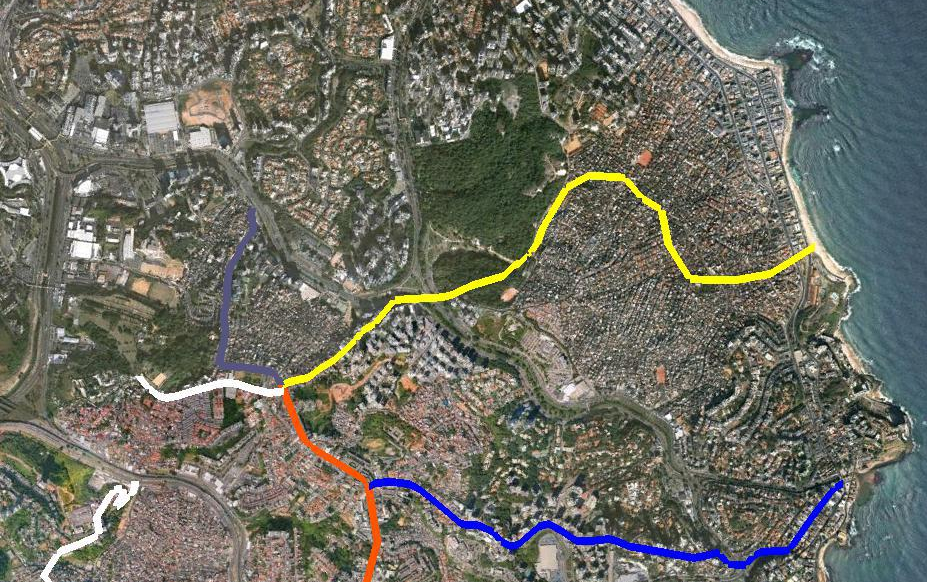
\includegraphics[width=0.7\textwidth]{3-cap2/complementos/mapas/armacaodalagoa-hoje.eps} 
\label{fig:armacaodalagoa-hoje}
}
\caption{Duas representações cartográficas do território correspondente às fazendas Alagoa, Amaralina, Santa Cruz, Ubarana e Pituba. Não foi possível avançar além do que o mapa mais antigo permitiu. \textbf{Fonte:} \citeonline{weyll_mappa_1851} e Google Earth.}
\end{figure}

A história fundiária destas cinco fazendas é inseparável, indissolúvel, indivisível. Limítrofes, integrantes do antigo morgado da Foz, seus antigos terrenos constituem, somados, a maior parte, quando não a totalidade, dos atuais bairros de Amaralina, Pituba, Nordeste de Amaralina, Santa Cruz, Rio Vermelho, Itaigara, Iguatemi, Chapada do Rio Vermelho e Vale das Pedrinhas.

Um dos grandes imóveis saídos do morgado da Foz foi a \textit{fazenda Alagoa}, localizada onde hoje estão os bairros do Rio Vermelho e Amaralina.

Quando ainda integrava o morgado foram construídos dentro dela, em 1768, um tanque de captação de água, um engenho (há muito desaparecido) e uma ermida \cite[p.~118]{campos_alagoa_1942}. A ermida, transformada em capela dedicada a Nossa Senhora dos Mares, ainda existe nos dias de hoje, incorporada ao Quartel de Amaralina, localizado no mesmo sítio onde se erguia a casa-grande do engenho.

Já desmembrada do morgado, a fazenda Alagoa foi adquirida em 1797 por Alexandre Teotônio de Sousa, tenente-coronel de granadeiros da guarnição de Salvador; alguns seus herdeiros remotos venderam-na em 1854 a José Álvares do Amaral\footnote{O primeiro sobrenome desta personagem histórica encontra-se grafado como ``Alves'' ou ``Álvares'' a depender da fonte. Foi mantida a grafia tal como foi encontrada.} \cite[p.~118]{campos_alagoa_1942}, com os seguintes limites constantes do \textbf{Livro Eclesial de Registro de Terras da Freguesia de Brotas}:

\begin{citacao}
Terreno de José Alves do Amaral

Em obediência ao despacho do senhor Vice-Presidente Missias de Leão, de 29 de abril de 1859, exarei o seguinte registro:

José Alves do Amaral, tendo o domínio útil da fazenda ``Alagôa'', situada nesta freguesia das Brotas, vem apresentala ao registro das terras. Principia o limite da dita fazenda, do lado da Ubarana, de propriedade útil do Major Manoel de Barros Paim, por um marco de pedra de cantaria collocado em mil setecentos e oitenta e nove na costa do mar em direção NO 35gº no qual se acha gravada a seguinte inscripção '1789', e partindo dahi no rumo que mostra o dito marco a encontrar a valla mestra divisória que passa nos fundos da dita fazenda Ubarana, e seguindo pela dita valla a encontrar a área nativa que limita com a fazenda ``Pituba'', de propriedade do Visconde do Rio Vermelho, e acompanhando a dita cerca até encontrar a estrada que conduz para a Cruz da Redempção em Brotas, dividindo sempre por esta estrada com a fazenda ``Santa Cruz'', de propriedade de Antonio Joaquim da Silva e Abreu, até o lugar chamado ``tanque'', e seguindo dahi pela valla mestra a desembocar no rio Camorogipe, e por este abaixo até sua foz no mar pela parte da Mariquita, confrontando por este lado com terras pertencentes ao Mosteiro de São Bento, tendo a dita fazenda toda a frente para o mar, pela costa as terras da dita fazenda [\textit{ilegível}] do senhorio direto Thomas da Silva Paranhos. Cumpre declarar que os limites da mencionada fazenda se encontram em litígio com os [\textit{ilegível}] confrontantes da Ubarana e Santa Cruz. Bahia, quatro de abril de mil oitocentos e cincoenta e nove. José Álvares do Amaral.

E nada mais continhão as declarações que me foram transmitidas. Brotas da Bahia, 3 de maio de 1859.

Vigº Ernesto de Olivª Valle\footnote{\textbf{BR BAAPB}, fundo Colonial, série Registros de Terra, livro 4675, f. 36 verso e 37.}
\end{citacao}

No mapa de \citeonline{weyll_mappa_1851} (cf. \autoref{fig:armacaodalagoa-1851}) há a indicação de uma ``Armação da Lagoa'', compatível com os relatos da existência de uma armação de pesca nesta fazenda desde os idos do século XVIII \cite[p.~120-121]{campos_alagoa_1942}. O mesmo mapa mostra uma estrada que a liga ao Largo de Brotas. Se seguirmos seu trajeto desde este largo até o mar e o compararmos com o trajeto de ruas atuais (cf. \autoref{fig:armacaodalagoa-hoje}), é plausível conceber alguns possíveis caminhos remanescentes desta antiga estrada\footnote{Com a base documental pesquisada até o momento é impossível descrever precisa e minuciosamente as ruas remanescentes desta estrada, e é possível mesmo que tal descrição documental sequer exista; a reconstituição desta estrada exigiria uma pesquisa \textit{in loco} com antigos moradores da Santa Cruz e do Nordeste de Amaralina para tentar recompor alguns traços perdidos desta estrada, profundamente modificada pela ocupação popular do território destes bairros, pelos loteamentos resultantes nos bairros de Amaralina e Pituba, e pela construção da avenida Juracy Magalhães e do Parque da Cidade.}

\begin{itemize}
\item Os dois caminhos saem do largo da Cruz da Redenção, descendo sua ladeira até o leito do rio Camorogipe, e o atravessam por meio de uma ponte (atualmente inexistente);
\item Uma primeira hipótese para um traçado remanescente desta estrada segue pela rua Onze de Novembro, ou Estrada da Santa Cruz, e daí pela rua do Futuro e pela avenida Nova República;
\item Uma segunda hipótese para o traçado corta caminho desde o leito do Camorogipe por dentro do atual Parque da Cidade, encontrando a avenida Nova República;
\item Da avenida Nova República o traçado segue encontrando-se com a rua Victorio Rossi para continuar pelo Beco da Cultura;
\item Uma linha imaginária ligaria o Beco da Cultura à rua Reinaldo de Matos, encontrando-se com a rua Cristóvão Ferreira;
\item Outra forma de ligar a avenida Nova República com a rua Cristóvão Ferreira seria sair da avenida para a rua Nova República, daí para a rua Valdomiro, depois para a travessa 20 de Junho, daí para as ruas do Areal e Ipanema, pela ruas Onze de Novembro e Francisco Sales até a rua dos Posseiros, e daí por uma linha imaginária até a rua Alto do Capim e, enfim, a rua Cristóvão Ferreira;
\item O caminho terminaria, por fim, na atual rua do Norte, ligada ao litoral por uma linha imaginária. 
\end{itemize}

É desta fazenda que deriva o loteamento, de final do século XIX, chamado \textit{Cidade Balneária Amaralina}, a ser detalhado no capítulo seguinte.

A compra da fazenda Alagoa foi fortemente contestada durante quase quarenta anos por Tomás da Silva Paranhos, comprador, como visto, do que restara do morgado da Foz \cite[p.~118]{campos_alagoa_1942}. Terminada a querela, diz um memorialista célebre que a fazenda teria sido rebatizada em 1912 como fazenda \textit{Amaralina} \cite[p.~118]{campos_alagoa_1942}; como se verá no capítulo seguinte, a documentação consultada durante esta pesquisa dá a entender que já na década de 1890 havia duas fazendas distintas, a \textit{Alagoa} e a \textit{Amaralina}.

Menos célebre que a fazenda Alagoa, a \textit{fazenda Santa Cruz} é assim descrita no \textbf{Livro Eclesial de Registro de Terras da Freguesia de Brotas}:

\begin{citacao}
Fazenda de Antonio Joaquim da Silva e Abreu

Antonio Joaquim da Silva e Abreu possue na freguesia de Nossa Senhora de Brotas da Capital da Bahia uma fazenda denominada ``Santa Cruz'', em terrenos proprios, aqual limita-se pelo nascente com a fazenda Ubarana, pelo poente com o rio Camorogipe, pelo norte com a fazenda Pituba e pelo sul com o mesmo rio Camorogipe na povoação da Mariquita. Bahia e Freguesia de Brotas, vinte e sete de novembro de mil oitocentos e cincoenta e oito. Antonio Joaquim da Silva e Abreu.

E nada mais continhão as declarações que me foram transmitidas. Brotas da Bahia, 27 de novembro de 1858.

Vigº Ernesto de Olivª Valle\footnote{\textbf{BR BAAPB}, fundo Colonial, série Registros de Terra, livro 4675, f. 36 e 36 verso.}
\end{citacao}

Não foi possível encontrar quaisquer outras referências a esta fazenda na documentação pesquisada, mas no capítulo seguinte se verá como esta fazenda foi loteada ao final da Primeira República.

A \textit{fazenda Ubarana} é assim descrita no \textbf{Livro Eclesial de Registro de Terras da Freguesia de Brotas}, num registro que se encontra severamente atingido pela ação do tempo:

\begin{citacao}
A fazenda denominada Ubarana, sita na f[regue]sia de N[oss]a Senhora de [Bro]tas, da Capital [da] Bahia, divide-se pelos la[do]s do Sul com a[s fa]zendas Alagôa e Santa Cruz, a saber [ilegível]dindo do [ilegível] da Ubarana do lado do Sul em [li]nha recta a Pedra da Marca pelo caminh[o] que vae para Brotas, afindar-se no rio Camorogipe, a encontrar do lado norte com a [ilegível] nativa de antigas árvores que faz a [divi]za com a fazenda da Pituba, descendo athe vizinhanças do mar, [ilegível] desta os limites [ilegível] referida fazenda do [ilegível] [ilegível]. Brotas, vinte e oito de novembro de mil oitocentos e cincoenta e nove. Manuel [ilegível] de Barros Paim.

E nada mais continhão as declarações que me foram transmitidas. Brotas da Bahia, 15 de janeiro de 1860.

Vigº Ernesto de Olivª Valle\footnote{\textbf{BR BAAPB}, fundo Colonial, série Registros de Terra, livro 4675, f. 40.}
\end{citacao}

Um resquício de memória desta fazenda ainda pode ser encontrado no nome da atual rua das Ubaranas, lindeira entre os bairros da Pituba e Amaralina, que corre paralela à avenida Manoel Dias da Silva entre as ruas Pará e Vandick Badaró.

Já a \textit{fazenda Pituba} tem seus limites assim descritos no \textbf{Livro Eclesial de Registro de Terras da Freguesia de Brotas}:

\begin{citacao}
Terras da Exmª Viscondessa do Rio Vermelho

Limites da legoa de terra que pertence a Excellentíssima Viscondessa do Rio Vermelho e o condomino seo filho Barão do Rio Vermelho. Na freguesia de Nossa Senhora das Brotas está a fazenda denominada Pituba em um [ilegível] de terras que pertenceu a Casa da Excellentíssima Marquesa de Niza, hoje ao Capitão Thomas da Silva Paranhos, e [ilegível] de posse por escriptura de foro perpetuo para a Excellentíssima Viscondessa do Rio Vermelho e seu filho o Barão do Rio Vermelho. Tem por limites a dita fazenda ao sul divide com a fazenda Ubarana, ao norte com terras do Engenho Santo Antônio, ao nordeste com terras de São Bento, onde está a Armação do Gregório, e a leste com o mar. Bahia, quinze de julho de mil oitocentos e cincoenta e nove. Barão do Rio Vermelho.

E nada mais continhão as declarações que me foram transmitidas. Brotas da Bahia, 15 de julho de 1859.

Vigº Ernesto de Olivª Valle\footnote{\textbf{BR BAAPB}, fundo Colonial, série Registros de Terra, livro 4675, f. 38.}
\end{citacao}

Como se pode inferir dos limites constantes nos registros de terra, a povoação da Mariquita era o ponto de convergência, e portanto de conflito, entre os limites das fazendas Santa Cruz e Alagoa. A deterioração do registro da fazenda Ubarana dificulta compreender os limites entre ela e as demais fazendas, pois a descrição de alguns marcos foi corroída pela tinta.



\subsection{Campinas e as terras dos Ladislau}

\begin{figure}[!htp]
\centering
\subfloat[Em 1851]{
\includegraphics[width=0.7\textwidth]{3-cap2/complementos/mapas/campinas-1851.eps} 
\label{fig:campinas-1851}
}
\  %espaco separador
\subfloat[Atualmente]{
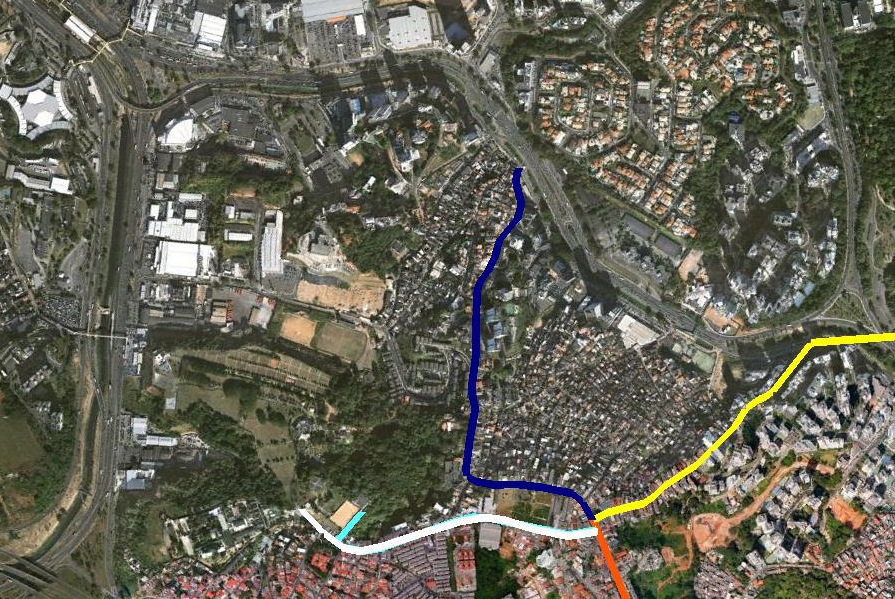
\includegraphics[width=0.7\textwidth]{3-cap2/complementos/mapas/campinas-hoje.eps} 
\label{fig:campinas-hoje}
}
\caption{Duas representações cartográficas do território correspondente às terras dos Ladislau. \textbf{Fonte:} \citeonline{weyll_mappa_1851} e Google Earth.}
\end{figure}

Toda a área que hoje conhecemos como \textit{Campinas de Brotas} era, no século XIX, de propriedade de integrantes da família \textit{Ladislau}, cujo patriarca, João Ladislau de Figueredo e Melo, vinha a ser sogro do mesmo José Álvares do Amaral reivindicante da fazenda Alagôa. O próprio nome da área -- Campinas -- deriva de duas das herdades da família.

A primeira delas era a fazenda Campina Grande:

\begin{citacao}
Fazenda Campina Grande

Rosa Ladislau de Figueredo e Melo e Virgínia Ladislau de Figueredo e Melo possuem em condomínio nesta Freguesia de Nossa Senhora das Brotas uma Fazenda denominada Campina Grande, em que há Engenho de fabricar assucar, e que comprehende a fazenda do mesmo nome Campina Grande, [ilegível] Carregado e Chacôco, terras proprias, que de [ilegível] [ilegível] um lado com a roça da dita Rosa Ladislau de Figueredo e Melo no lugar da Cruz da Redempção e com outra denominada Campina Pequena de dona Michelina Ladislau e Silva e dona Joanna Fausta Ladislau e Silva, de outro com terras do Matatu de José Antonio Pinto pelo riacho de mesmo nome, e mais com terras do Girão de Joaquim Caetano de Almeida Couto, ou quem mais direito for, pelo riacho Camorogipe, outra com terras que forão de dona Maria de Argôlo, e com as do Engenho Santo Antônio da Viscondessa do Rio Vermelho e sua filha dona Judith Constança da Cunha, pelo dito Camorogipe, e pelo outro com a estrada que sobe da ponte do mesmo Camorogipe e com terras que forão de João Paulo e seu irmão Fabião. Esta declaração vae por uma de nós feita e por ambas assignada. Bahia e Freguesia de Nossa Senhora das Brotas, primeiro de junho de mil oitocentos e cincoenta e oito. Rosa Ladislau de Figueredo e Melo, Virgínia Ladislau de Figueredo e Melo.

E nada mais continhão as declarações que me foram enviadas. Brotas da Bª, 5 de junho de 1858.

Vigº Ernesto de Olivª Valle\footnote{\textbf{BR BAAPB}, fundo Colonial, série Registros de Terra, livro 4675, f. 4 verso e 5.}
\end{citacao}

A outra, a fazenda Campina Pequena:

\begin{citacao}
Roça Campina Pequena

Michelina Ladislau e Silva e Joanna Fausta Ladislau e Silva possuem nesta Freguesia de Nossa Senhora das Brotas uma roça denominada Campina Pequena com casa de vivenda e outras benfeitorias, terras próprias, e que se divide pela frente com terras de Raphael e José Joaquim, e por outro lado com a Quinta das Beatas pelo riacho que a separa, por outro com a estrada que entra para o Engenho da Campina Grande, e pelo fundo com terras do mesmo Engenho. Esta declaração vae feita por uma de nós e por ambas assignada. Bahia e Freguesia de Nossa Senhora das Brotas, primeiro de junho de mil oitocentos e cincoenta e oito. Michelina Ladislau e Silva, Joanna Fausta Ladislau e Silva.

E nada mais continhão as declarações que me forão enviadas. Brotas da Bahia, 4 de junho de 1858.

Vigº Ernesto de Olivª Valle\footnote{\textbf{BR BAAPB}, fundo Colonial, série Registros de Terra, livro 4675, f. 5 e 5 verso.}
\end{citacao}

No mapa de \citeonline{weyll_mappa_1851} (cf. \autoref{fig:campinas-1851}), vê-se nitidamente que o ``Engº'' marcado perto de ``Prambeé'' corresponde muito proximamente à descrição documental do Engenho Campina Grande, situado na baixada hoje correspondente à rua Santiago de Compostela. No cume logo abaixo do ``Engº'' no mapa, onde hoje se situam  o cemitério Jardim da Saudade e o Abrigo Salvador, tem início uma estrada que corresponde à atual rua Campinas de Brotas. À atual rua Teixeira Barros corresponde a antiga Estrada do Beijú; se o mapa de Weyll continuasse mais ao leste, seria possível observar como esta estrada se unia à Estrada das Armações no trecho onde se cruzam, hoje, as avenidas Paulo VI e Antônio Carlos Magalhães. 

Em 1845 se anunciava a venda, no Campina Grande, ``distante desta cidade tres quartos de legoa'', de ``capim bom e verde, já cortado, a 120 a arroba''\footnote{\textbf{O Mercantil}, 27 set. 1845, p. 4.}. Notícia de prisão efetuada em suas matas indica que o engenho Campina ainda existia enquanto tal em 1881\footnote{\textbf{O Monitor}, 10 jun. 1881, p. 1.}.





\subsection{A Estrada de Brotas e seus arredores}

\begin{figure}[!htp]
\centering
\subfloat[Em 1851]{
\includegraphics[width=0.4\textwidth]{3-cap2/complementos/mapas/estbrotas-1851.eps} 
\label{fig:estbrotas-1851}
}
\  %espaco separador
\subfloat[Atualmente]{
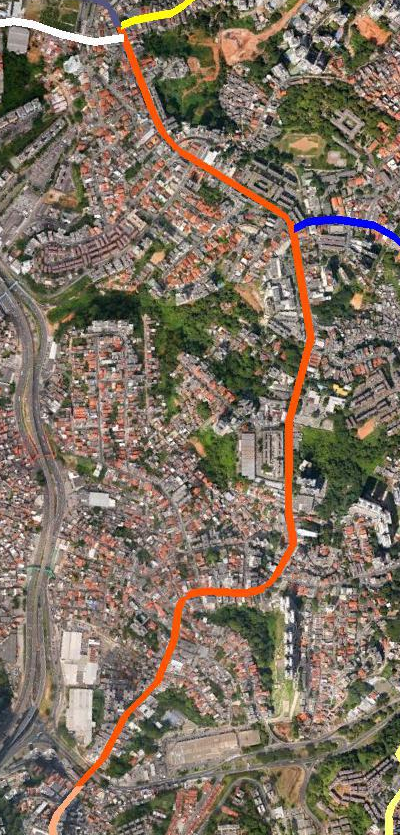
\includegraphics[width=0.4\textwidth]{3-cap2/complementos/mapas/estbrotas-hoje.eps} 
\label{fig:estbrotas-hoje}
}
\caption{Duas representações cartográficas do território correspondente à Estrada de Brotas (atual av. D. João VI). \textbf{Fonte:} \citeonline{weyll_mappa_1851} e Google Earth.}
\end{figure}

No século XVIII saía do Portão da Piedade uma estrada então conhecida como \textit{Caminho Grande}, correspondente ao que veio depois ser a \textit{Estrada de Brotas}, atual Avenida D. João VI; era por aí que se partia da cidade ao Rio Vermelho, passando pelo paço do Acupe, integrante do morgado da Casa da Torre \cite[p.~85]{campos_brotas_1942}. Patente de sargento-mor da freguesia de ``Nossa Senhora de Brotas do Caminho Grande'' concedida a Veríssimo de Campos de Carvalho em 1725 \cite[p.~114]{texmel_manusbn_1896} mostra como era conhecida a freguesia em seus primórdios.

Infelizmente não foi possível encontrar registros seguros do traçado completo do Caminho Grande, exceto por uma referência que o qualificou como `perigoso'' e disse passar ele ``pela Lapa e atual Campo da Pólvora, pela crista dos montes e pelos divisores de águas, passando em Fonte Nova e por Brotas até aquele ponto da costa oceânica'' \cite[p.~488]{sampaio_salvador_2016}. Com base no mapa de \citeonline{weyll_mappa_1851} (cf. \autoref{fig:estbrotas-1851}), pode-se conjecturar, entretanto, que a ligação entre a Piedade e o atual Largo do Paranhos, onde tinha início a Estrada de Brotas, fosse feita pelo trecho da atual avenida Joana Angélica que vai até a ladeira da Fonte Nova e por esta própria ladeira, chegando, através da atual ladeira dos Galés, até o referido largo, completando assim o primeiro trecho. Daí em diante, pode-se apenas conjecturar, inconclusivamente, por onde o Caminho Grande desceria rumo ao Rio Vermelho.

O jornal quinzenal \textbf{A Lei}, num breve perfil biografico, indicou que em 1848 o brigadeiro Evaristo Ladislau e Silva ``concorreu para o melhoramento da estrada de Brotas''\footnote{\textbf{A Lei}, ano 2, nº 2, fev. 1877, pp. 2-3.}; certamente terá a ver com o fato de que entre 1848 e 1849 a presidência da província investiu 2:269\$344 na Estrada de Brotas, comprometendo-se a investir outros 5:000\$000 em melhoramentos na via; investiu também 1:414\$000 no encanamento do rio Camorogipe, empenhando-se a investir outros 177:539\$000 na mesma finalidade \cite{bahia_rpe_1849}.

Como a Estrada de Brotas era -- e continua sendo, se somarmos as atuais ruas que estão sobre seu antigo leito -- muito comprida, é preciso fazer como os da época e subdividi-la em alguns pontos notáveis e cercanias.

O primeiro deles é o \textit{Largo de Brotas}, existente desde a fundação da igreja matriz. Em 1882 uma casa posta a leilão nesta localidade foi assim descrita e avaliada:

\begin{citacao}
...uma casa ao largo da matriz de Brotas, n. 14, com 5 metros e 46 centimetros de frente, que é dobrada e de azulejos, com porta e 2 janellas, sala feichada, 3 quartos, sala de jantar, cosinha, quintal e sotão, em terreno proprio [\dots]\footnote{\textbf{Diário da Bahia}, 30 set. 1882, p. 3.}.
\end{citacao}

Apesar de um célebre memorialista afirmar que o \textit{largo da Cruz da Redenção}, até hoje existente, foi mandado abrir em 1841 na Estrada de Brotas pelo coronel João Ladislau de Figueredo e Mello, dono do engenho Campinas \cite[p.~88]{campos_brotas_1942}, já se encontra anúncios de venda de roça na mesma localidade em 1838\footnote{\textbf{Correio Mercantil}, vol. 3, nº 583, 19 out. 1838, p. 4.}.

Em 1882 uma casa posta a leilão nesta localidade foi assim descrita e avaliada:

\begin{citacao}
Uma casa situada à rua da Redempção, freguezia de Brotas, com 3 metros e 30 centimetros de frente, e n'esta uma porta e janella, sala, dous quartos, sala de jantar em commum com a cosinha, pequeno quintal; divide-se por um lado com casa do intestado e pelo outro com Luiz Mendes, avaliada por 100\$000\footnote{\textbf{Diário da Bahia}, 3 jan. 1889, p. 2.}.
\end{citacao}



Caetano Vicente de Almeida Galião, juiz de paz do segundo distrito da Sé em 1835, possuía um pequeno engenho e uma pequena fazenda em Brotas \cite[p.~239]{REIS2004males}.

\subsubsection{Cruz das Almas}

Já em 1870, um certo Miguel dos Santos Prates vinha a público agradecer aos que acompanharam o cortejo fúnebre de seu pai desde sua casa, na Estrada da Cruz das Almas, até o cemitério de Brotas\footnote{\textbf{O Monitor}, 20 jun. 1870, p. 3}

\subsubsection{Cemitério de Brotas}

Em 1871 o cemitério da freguesia de Brotas já demandava ser alargado\footnote{\textbf{Jornal da Bahia}, ano XIX, nº 5.446, 22 set. 1871, p. 1}, e em 4 de julho de 1876 o juiz e mesário da irmandade do Santíssimo Sacramento de Nossa Senhora de Brotas requereu ao administrador do cemitério 30 metros quadrados de terreno devoluto para a construção de carneiros para a irmandade\footnote{\textbf{O Monitor}, 16 jul. 1876, p. 2}. Em 1879 a presidência da província transferiu a administração do cemitério para a Câmara Municipal por meio da lei 1.943, de 26 de agosto do mesmo ano\footnote{\textbf{O Monitor}, 30 ago. 1879, p. 1.}.

\subsubsection{Estrada e Alto do Beijú}


\subsection{A fazenda Boa Vista e seus arredores}

\begin{figure}[!htp]
\centering
\subfloat[Em 1851]{
\includegraphics[width=\textwidth]{3-cap2/complementos/mapas/boavista-sangradouro-1851.eps} 
\label{fig:boavista-sangradouro-1851}
}
\  %espaco separador
\subfloat[Atualmente]{
\includegraphics[width=\textwidth]{3-cap2/complementos/mapas/boavista-sangradouro-hoje.eps} 
\label{fig:boavista-sangradouro-hoje}
}
\caption{Duas representações cartográficas do território correspondente à fazenda Boa Vista (atual Engenho Velho de Brotas) e ao Sangradouro (atual Santo Agostinho). \textbf{Fonte:} \citeonline{weyll_mappa_1851} e Google Earth.}
\end{figure}

O mapa de \citeonline{weyll_mappa_1851} mostra ainda uma longa estrada saindo das terras da Boa Vista em direção a uma estrada que corresponde à atual avenida Cardeal da Silva. Remanescentes desta estrada são as ruas Almirante Alves Câmara e Padre Luiz Figueira, no Engenho Velho de Brotas, e Sérgio de Carvalho, no Vale da Muriçoca; mais ou menos no ponto onde a Sérgio de Carvalho faz esquina com a atual av. Edite, também no Vale da Muriçoca, o mapa de Weyll indica uma ponte sobre um riacho, e daí em diante a estrada seguia um curso hoje inexistente, que terminava aproximadamente na altura da atual Ladeira das Carmelitas, na Federação. Seria esta a Estrada da Boa Vista, estendendo-se desde o Largo dos Paranhos até a atual Cardeal da Silva?

\subsubsection{Moinho}



\subsubsection{Capela do Deus Menino}



\subsubsection{Dique Pequeno}



\subsubsection{Monte de Belém}



\subsubsection{Porto dos Saveiros}



\subsubsection{Estrada da União}



\subsection{A Estrada Dois de Julho}

\begin{figure}[!htp]
\centering
\subfloat[Em 1851]{
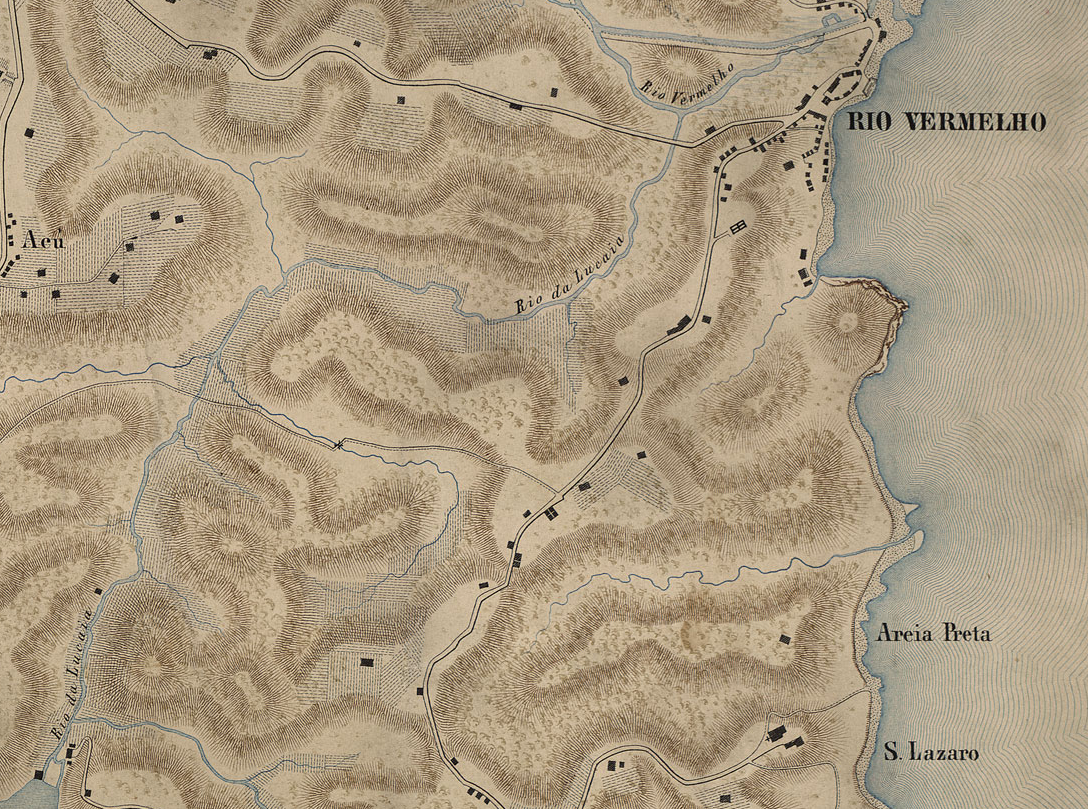
\includegraphics[width=0.7\textwidth]{3-cap2/complementos/mapas/e2j-1851.eps} 
\label{fig:e2j-1851}
}
\  %espaco separador
\subfloat[Atualmente]{
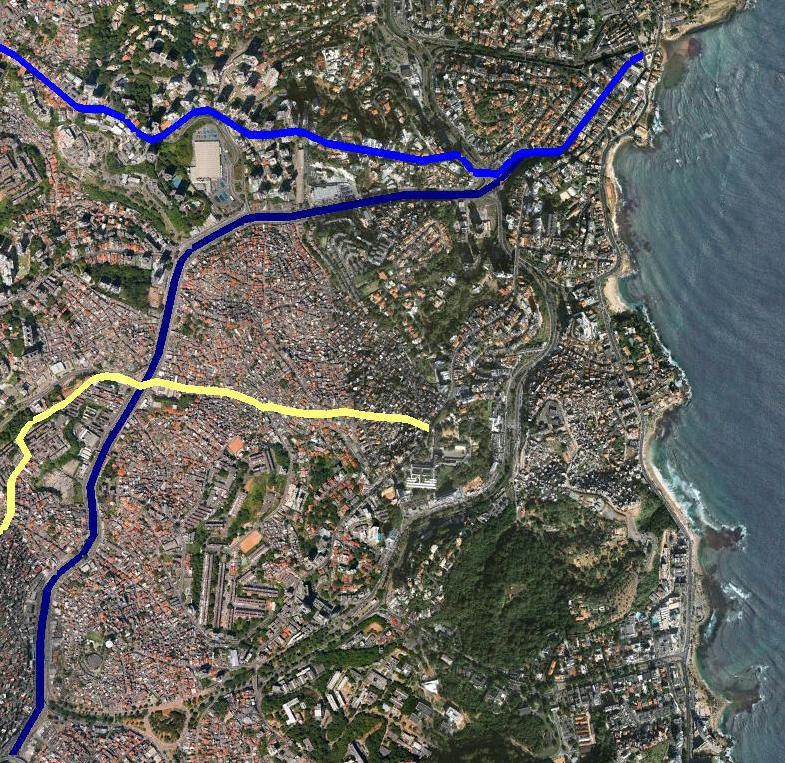
\includegraphics[width=0.7\textwidth]{3-cap2/complementos/mapas/e2j-hoje.eps} 
\label{fig:e2j-hoje}
}
\caption{Duas representações cartográficas da Estrada Dois de Julho (atual av. Vasco da Gama). Em 1851 ela não estava construída, mas corresponde ao leito do rio Lucaia. \textbf{Fonte:} \citeonline{weyll_mappa_1851} e Google Earth.}
\end{figure}

Em 10 de maio de 1879 o presidente da província ordenou ao diretor de obras públicas 

\begin{citacao}
\dots lavrar contracto n'essa repartição com o Commendador Giusto Ariani para o serviço de deseccação do terreno na estrada Dous de Julho, entre a fábrica de lapidação de diamantes pertencente aos negociantes Costa Pinto \& Filhos e a ladeira que segue para Brotas, e bem assim para a canalisação da parte do riacho Lucaia entre aquelles dous pontos\footnote{\textbf{O Monitor}, 3 jun. 1879, p. 1.}.
\end{citacao}
\subsection{O Matatu Grande, o Matatu Pequeno, Quinta das Beatas e arredores}\label{subsec:matatubeatas}

Em 17 de junho de 1799 o Conselho Ultramarino deu parecer favorável a requerimento de porte de armas defensivas feito pelo capitão Pedro Gomes Ferreira; o militar residia ``na sua fazenda do Matatu'' \cite[p.~228]{castralmeida_ultramar_1914}, indicando que já no século XVIII a área era reconhecida por este nome. 

Há duas versões para a etimologia do topônimo. A primeira e mais conhecida diz ser ele de origem tupi, significando ``mata escura'', ``floresta negra'' \cite[p.~281]{sampaio_tupi_1987}. A segunda, menos conhecida, diz que se trata de um africanismo de origem bantu, significando ``lugar deserto, isolado'' \cite[p. 46]{dorea_ruas_2006}. Qualquer das duas versões, seja pela existência de mata fechada, seja escassez populacional, passam a impressão de um lugar distante, ermo, pouco povoado, e é bem possível que assim o fosse no século XVIII quando encontramos a primeira referência ao nome; no século XIX, entretanto, o \textbf{Livro Eclesial de Registro de Terras da Freguesia de Brotas} indica a existência de muitos pequenos proprietários de terras na área, sendo ela a que mais tem registros fundiários em toda a freguesia\footnote{\textbf{BR BAAPB}, fundo Colonial, série Registros de Terra, livro 4675.}.

No mapa de \citeonline{weyll_mappa_1851}, lido no sentido NNE-SSE (cf. \autoref{fig:matatu-1851}), a área é representada por três cumeadas. 

\begin{figure}[!htp]
\centering
\subfloat[Em 1851]{
\includegraphics[width=0.7\textwidth]{3-cap2/complementos/mapas/matatu-1851.eps} 
\label{fig:matatu-1851}
}
\  %espaco separador
\subfloat[Atualmente]{
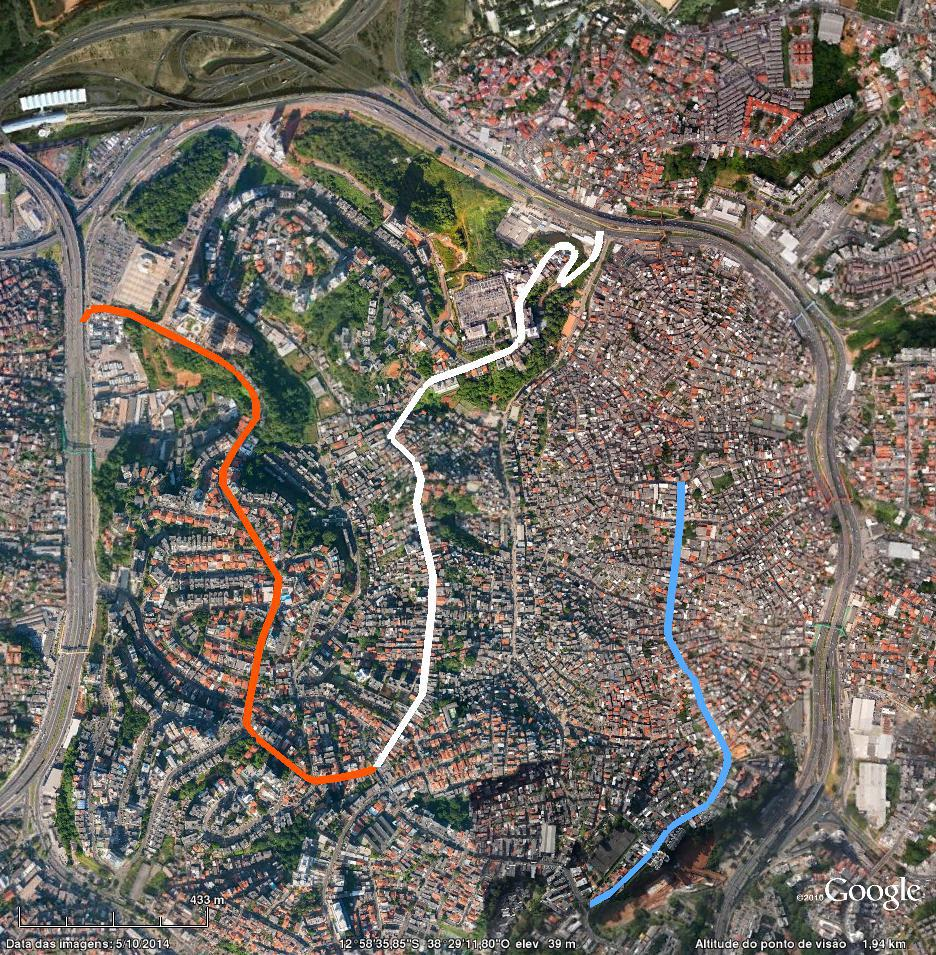
\includegraphics[width=0.7\textwidth]{3-cap2/complementos/mapas/matatu-hoje.eps} 
\label{fig:matatu-hoje}
}
\caption{Duas representações cartográficas do Matatu, mostrando a rua da Valla (atual av. Heitor Dias), a Estrada da Pólvora (atual rua Raul Leite), a Estrada do Matatu Grande (atual rua Luiz Anselmo) e a Quinta das Beatas (atual Cosme de Farias). \textbf{Fonte:} \citeonline{weyll_mappa_1851} e Google Earth.}
\end{figure}

 A terceira tem uma estrada, correspondente à atual rua Cosme de Farias, que vai dar na ``Quinta das Biatas''
 
 . No mesmo mapa é possível encontrar símbolos indicativos de construções pontilhando a cumeada do Matatu Grande, embora a cumeada onde se localiza a Casa da Pólvora apresente-se pouco povoada, assim como a da Quinta das Beatas.

Novamente lendo o mapa de Weyll no sentido NNE-SSE (\autoref{fig:matatu-1851}), quatro rios escavam os vales circundantes destas cumeadas. Temos em primeiro lugar o \textit{rio das Tripas}, afluente do Camaragipe, vizinho ao qual corria a rua da Vala, no trecho correspondente à atual avenida Heitor Dias. O segundo rio é indicado por Weyll como sendo o \textit{Santo Antônio}, hoje um esgoto \cite[p.~136]{santos_aguas_2010} que corre quase paralelamente à atual rua do Baixão. O terceiro rio é o \textit{Córrego das Beatas} \cite[p.~158]{santos_aguas_2010}, correspondente, grosso modo, à atual Baixa do Matatu, também transformado em esgoto. O Córrego das Beatas é afluente do rio \textit{Bonocô}, que no mapa de \citeonline{weyll_mappa_1851} separa a Quinta das Beatas da cumeada cortada pela Estrada de Brotas.

Dado o grande tamanho da área analisada, será preciso subdividi-la nos pontos notáveis e nomes pelos quais era conhecida na época, atualizando-os quando necessário.

A porta de entrada para o Matatu, no sentido de quem vem da Ladeira dos Galés, é o \textit{largo do Paranhos}, assim batizado em homenagem ao já mencionado latifundiário Tomás da Silva Paranhos.

Em 1879 foi anunciado o leiloamento de uma roça de propriedade de Herman e Sophia Both, penhorada pela Sociedade de Commercio, localizada no largo do Paranhos, descrita no anúncio a seguir. bserve-se com detalhe a estrutura e o valor do imóvel à venda; trata-se de fazenda bem constituída, de gente abastada o suficiente para ter inquilinos:

\begin{citacao}
Uma roça em terreno proprio, na freguezia de Brotas, largo denominado de Paranhos, tendo a frente para o mesmo largo, dividindo-se pelo lado direito com a roça que foi do Bacharel Firmino Duarte Gameleira; pelo esquerdo, com a estrada que vai para a Quinta das Beatas; e pelo lado direito continuando de fundo à frente com terreno que foi do dito Bacharel Gameleira onde vae acabar. Medida a frente da roça, acha-se n'ella 336m 10c; do canto que vira para a estrada da Quinta das Beatas até encostar na roça que foi do Bacharel Gameleira, havendo n'este lado 143m 60c; de terreno, com o fundo de 43m 25c, que foram dados por aforamento a diversos, pelos executados, de modo que fica a frente propriamente dita da roça com 180m 50c, desde o terreno aforado até a esquina para a estrada das Boiadas, e essa frente está fechada por muros de boa construcção, tendo um portão de ferro por onde é a entrada principal para a roça e casa de morada. A entrada do portão para a casa é guarnecida de perfeitas cercas de pitangueiras, que terminam em 2 carramanchões sobre pilastras de pedra de cantaria; dentro das cercas de pitangueiras existem diversas arvores, como saputizeiros, abacateiros, laranjeiras etc., havendo no lado esquerdo da mesma roça diversas divisões formadas por cercas de pitangueiras, e em todos esses lotes diversas arvores, como as declaradas, cuja quantidade é a seguinte:

Na parte cultivada da roça existem: 60 jaqueiras, 73 mangueiras, 193 laranjeiras, 10 pes de fructa pão, 8 cajazeiras, 8 abacateiros, 24 saputizeiros, 23 coqueiros, 2 genipapeiros, 1 tamarindeiro, 4 [ilegível] de parreira, sendo algumas de pés direitos de cantaria, 1 brejo que termina em uma ribanceira, onde existe uma capoeira para corte de madeira, 1 telheiro fechado por paredes de taboas com uma machina à vapor em bom estado, serve para conduzir agua a um deposito junto á propriedade da morada, a qual agua é puxada por um encanamento de ferro, de um deposito de pedra e cal cimentado e coberto tambem com telheiro, 1 banheiro fechado por paredes de pedra e cal, e coberto de telhas, com 2 portas e 3 torneiras de bronze.

Uma casa de campo de gosto antigo com varandas fechadas por frontoes, e n'elles peitoris, tendo no lado direito da varanda, 1 oratorio de celebrar missa. A entrada é por uma porta entre 4 janelas, com sala aberta que occupa a porta e 2 janelas, e 1 gabinete em cada lado, tendo cada gabinete 1 janella, e a entrada para o interior da casa é pela sala de jantar que dá em 1 salão, havendo de cada lado deste 1 corredor, com diversos repartimentos que são: 10 quartos, dispensa e cozinha, toda construida de pedra e cal e de gosto antigo. Depois desses repartimentos um grande salão de pedra e cal, com paredes dobradas, feito muito depois da casa, e de gosto moderno, rodeado de janellas de vidraças, isto é, com janelas de vidraças no fundo e no lado, e a parte por onde abre-se para um terraço d'onde desce-se para o centro da roça por uma escada de pedra, sobre este salão há um sotão para onde sobe-se por uma escada interna, tendo o mesmo sotão 4 divisões eguaes (4 grandes quartos ou 4 pequenas salas) cada uma com 2 janelas de vidraças, pelo que é o dito sotão rodeado de janellas, tanto a sala da frente como os quartos e o salão são forrados; a sala e os mais commodos terreos são cimentados, e o sotão é de lages de pedra; a casa descripta e o seu acrescimo (salão e sotão) tem de frente 12m60c de comprimento de frente a fundo 38m30c, cinco senzalas cobertas de telha em estado de reparo, dentro da roça, com 25m90c de frente; e em seguimento as mesmas senzalas 2 cazinhas que estão alugadas, e cujos inquilinos aproveitam-se na entrada e sahida do porão da cocheira.

Em frente ás senzalas e encostado ao muro da roça, existe um grande armazem, onde foi antiga estribaria, que ainda hoje tem em parte mangedouras, armazem esse que é coberto de telhas e precisa de reparos. A roça, casa e mais dependencias as avaliaram em 10:000\$000 [\dots]\footnote{\textbf{O Monitor}, 10 dez. 1879, p. 2.}.
\end{citacao}

O.

Passado o largo do Paranhos, chega-se de imediato à estrada que os contemporâneos chamavam das \textit{Pitangueiras}, curto trecho entre o largo e a estrada do Matatu Pequeno, hoje conhecida como Rua Barros Falcão. 

A primeira notícia encontrada acerca da existência do ``povoado das Pitangueiras'' é de 1871, numa situação polêmica. Uma escola primária masculina havia sido recentemente removida para este povoado, medida elogiada pelo rápido crescimento das turmas e pela abertura de turmas noturnas para artistas-operários\footnote{\textbf{Jornal da Bahia}, ano XIX, nº 5.445, 21 set. 1871, p. 1.}; tal remoção, entretanto, teria prejudicado os moradores do largo de Brotas, que só em 1876, depois de muito peticionar ao governo provincial, conseguiram deste a contratação de professores particulares para meninos e meninas da localidade\footnote{\textbf{O Monitor}, 3. set. 1876, p. 1.}. A situação, entretanto, ainda não havia melhorado em 1877, como se vê neste clamor assinado por um ``Amigo das Letras'':

\begin{citacao}
\textbf{Aos senhores deputados provinciaes}

Pedimos aos senhores deputados provinciaes que se dignem lançar suas vistas sobre a freguezia de Brotas desta capital, que muito necessita de duas escolas, sendo uma para cada sexo. As cadeiras dessa freguezia acham-se funcionando no logar denominado Pitangueiras -- de forma que um grande numero de crianças de um e outro sexo que moram no largo de Brotas e no Engenho Santo Antonio não podem receber a instrucção primaria.
Bahia, 18 de março de 1877\footnote{\textbf{O Monitor}, 22 mar. 1877, p. 3.}.
\end{citacao}

Ainda em abril de 1877 a situação da escola em Pitangueiras parecia periclitante, pois sua transferência para um extremo da freguesia resultara em grande evasão escolar\footnote{\textbf{O Monitor}, 28 abr. 1877, p. 1.},

Não é difícil deduzir desta situação que Pitangueiras era localidade de difícil acesso para os moradores do largo de Brotas e do Engenho Santo Antônio; pode-se igualmente deduzir a hipótese de que estas duas últimas localidades tivessem, entre 1871 e 1877, número de moradores maior que o de Pitangueiras. 

É certo, entretanto, que Pitangueiras concentrava razoável infraestrutura urbana, pois anúncio de casa a alugar nesta localidade em 1879 indicava ter a mesma ``os commodos necessarios para familia e encanamento de gaz''\footnote{\textbf{O Monitor}, 17 maio 1879, p. 2.}. Na mesma linha vai o anúncio de leiloamento dos seguintes imóveis, todos de bom padrão para a época:

\begin{citacao}
\textbf{Bens de raiz -- }Uma casa abarracada sita à rua das Pitangueiras, freguesia de Brotas, de n. 159, edificada em terreno proprio, com 8 metros e 10 centimetros de frente e 24 metros e 10 centimetros de fundo que dá para a rua Sete de Setembro, tendo de lado que dá para o beco 18 metros e 80 centimetros, com terraço na frente com gradil de ferro; a casa tem 2 janellas de peitoril e porta de vidraça no centro, 5 janellas do lado, sala de espera com porta para o becco, sala de visita, 2 quartos, salla de jantar e dispensa, e toda ella forrada, salla de gommar e cozinha, 3 quartos no quintal, lenheiro e sofás de cimento e concha para recreio, quintal todo murado com um portão para a dita rua, sotão com sala e 3 quartos, paredes todas dobradas, divide-se por um lado com casa do mesmo casal, avaliada por 4:000\$000.

Uma casa abarracada sita na dita rua e freguezia, de n. 157, edificada em terreno proprio, com 7 metros e 80 centimetros de frente com terraço e gradaria de ferro, com 2 janellas e porta no centro, sala de frente, 3 quartos, sala de jantar e toda ella forrada, dispensa, cozinha, sala de gommar com 2 quartos no quintal, sotão com janellas para a frente e fundo, com sala e 3 quartos, quintal todo murado com porteira para a rua Sete de Setembro, divide-se a casa por outro lado com casa do casal, avaliada por 3:000\$000.

Um terreno sito à rua Sete de Setembro, na dita freguezia, tendo de comprimento 38 metros, dividindo-se pelo fundo com terrenos do Hospital Militar, tendo diversas casas n'elle edificadas, avaliado cada metro por 15\$000 e todos por 570\$000 [\dots]\footnote{\textbf{O Monitor},3 out. 1879, p. 2.}.
\end{citacao}

Passado trecho da estrada das Pitangueiras, chega-se a uma esquina onde se abre a estrada que conduz à \textit{Quinta das Beatas}. A fazenda que ficou conhecida por este nome, no atual bairro de Cosme de Farias, tem sua descrição no \textbf{Livro Eclesial de Registro de Terras da Freguesia de Brotas} extremamente danificada pela ação do tempo:

\begin{citacao}
Quinta das Beatas

[ilegível] fazenda denominada Quinta das Beatas é propriedade do Recolhimento do Senhor Bom Jesus dos [Perd]oens, está situada na freguesia de Nossa Senhora  [de] Brotas, confina pelo nascente com a fazenda de[no]minada Campina, dos herdeiros do coronel João Ladis[la]u de Figueredo, e Matatu Grande, pertencente ao [ilegível] Pinto, pelo poente com a roça do tenente[-coron]el Pinheiro e com o capitão Paranhos, pelo sul [com] a roça de Amorim Vianna, com a Torre e com a [ilegível] e pelo norte com o Matatu pequeno e com [ilegível] [ilegível] Paranhos. Bahia, dezesseis de março de [mil oitocentos e] sessenta. Anna Maria Magdalena Re[jente]. 

[E nada mais] se continha em as ditas declarações [que me for]am enviadas.

Brotas da Bª, 20 de [março de 1860].

Vigº Ernesto de Olivª Valle\footnote{\textbf{BR BAAPB}, fundo Colonial, série Registros de Terra, livro 4675, f. 40 verso.}
\end{citacao}

A antiga sede da fazenda, a julgar pelo que mostra o mapa de \citeonline{weyll_mappa_1851}, estaria em algum lugar no trecho da atual rua Cosme de Farias situado entre as esquinas das atuais ruas Jaguarari e Lima Durval.

A relação entre o Recolhimento dos Perdões e a Quinta das Beatas é um dos mais acabados exemplos do \textit{rentismo}, sustentáculo econômico de tantas ordens religiosas católicas desde a fundação de Salvador até o presente. Na tentativa de fazer subir sua ordem na hierarquia eclesial (de \textit{recolhimento} a \textit{casa de professas}), mais especificamente como parte da ordem das carmelitas calçadas, as irmãs recolhidas nos Perdões argumentaram por todos os meios possíveis, incluindo os econômicos; em 1820 alegaram possuir, além do 

\begin{citacao}
recato e honestidade em que vivião, o possuirem renda sufficiente de 28 predios urbanos, a grande roça de nossa Sra. da Conceição das Brotas, mais conhecida por \textit{quinta das beatas}, não pequena porção de terreno arrendado e aforado, além de 16:000\$000 rs. em dinheiro de varios legados [\dots] \cite[p.~231]{accioli_memorias5_1937}.
\end{citacao}

Embora o relato apresente mais uma das tentativas frustradas de ascensão hierárquica das recolhidas, deixou evidente seu poder econômico. Pequeno, se comparado ao dos beneditinos, por exemplo \cite{bento_tombo_1945}, mas, mesmo assim, \textit{poder}.

Por ser de 1851, o mapa de Weyll ainda não poderia mostrar a \textit{Ladeira do Fabrício}, conhecida a princípio como \textit{Estrada do Sangradouro ao Matatu}, que corresponde ao trecho que inicia na Rua dos Tupys, esquina com a atual Rua do Sangradouro, e segue pela Ladeira dos Bandeirantes até encontrar-se com a estrada para o Matatu no local onde hoje a Ladeira dos Bandeirantes faz encruzilhada com as atuais ruas Alberto Torres, Barros Falcão e Amazonas. Esta ladeira foi mandada abrir em 1876 pelo governo provincial, em obras supervisionadas por uma comissão ``composta do Tenente-Coronel Fabricio Alves de Araujo, Bacharel Firmino Duarte Pacifico Gameleira e Negociante Manuel da Silva Pereira Guimarães'' \cite[p.~23]{bahia_1878}. A obra já se encontrava concluída no ano seguinte, sendo alargada de seus 8,8m originais para a largura de 11m e tendo recebido na mesma ocasião ``declives menos fortes'' \cite[p.~228]{bahia_1879}, e em 1885 recebeu calçamento \cite[p.~11]{bahia_1885}.

Passada a entrada da Quinta das Beatas, a estrada das Pitangueiras segue adiante até surgir uma bifurcação entre a \textit{Estrada do Matatu Grande} (direita) e a \textit{Estrada do Matatu Pequeno} (esquerda)\footnote{Há indicação de que a Estrada do Matatu Grande corresponderia às atuais ruas Luiz Anselmo e Raul Leite, e a Estrada do Matatu Pequeno à atual rua Barros Falcão \cite[p.~124]{valladares_beaba_2012}; a indicação, entretanto, não faz sentido, porque a junção da Luiz Anselmo com a Raul Leite resultaria numa grande via, em forma aproximada de ``U'', que reuniria as cumeadas dos morros que no mapa de \citeonline{weyll_mappa_1851}, contemporâneo das antigas denominações, são separadas como ``Matatu Grande'', à direita, e ``Casa da Povora'', à esquerda. Na falta de documentos comprobatórios da mudança toponímica, não encontrados até onde foi possível avançar na pesquisa ora exposta, parece muito mais plausível que a Estrada do Matatu Grande corresponda à rua Luiz Anselmo e a Estrada do Matatu Pequeno à rua Raul Leite.}.

O \textit{Matatu Grande} situa-se ao final de uma estrada que corresponde em grande parte à atual Rua Luiz Anselmo. Sucessivos anúncios de venda de capim na ``fazenda Matatú Grande''\footnote{\textbf{Gazeta da Bahia}, várias edições entre 1879 e 1886.} dão a entender que se trata de uma só fazenda.

O anúncio do leiloamento da roça de Bernardo Pires da Costa Chastinet descreve assim a propriedade:

\begin{citacao}
Uma roça e casa na estrada do Matatú Grande, na freguezia de Brotas, tendo quarenta metros e vinte centimetros de terreno de frente, e dentro três pés de mangueiras, três pés de jaqueiras, coqueiros, cajueiros, bananeiras, avaliado cada metro do terreno a cinco mil réis, e todos por duzentos e um mil réis. Os arvoredos todos avaliados em quarenta mil réis.

Uma casa terrea edificada na frente da estrada, e mede nove metros de frente, de paredes de taipa, tendo porta e duas janellas, estando do lado do norte parte da parede cahida; tem sala aberta e escorada, um quarto e cozinha com porta para o fundo, e toda a casa é feita da mesma construcção da frente, está toda coberta de telha, avaliada por sessenta mil réis; todo o terreno é proprio e divide pelo fundo com o rio Baixão que encosta as terras pertencentes ao proprietario Vidal de Oliveira, e pelo lado do norte com a roça de Thomé de Sant'Anna e pelo sul com terras de Miguel dos Anjos, sendo todo o terreno de ribanceira desde a frente até o brejo, avaliado tudo em tresentos e um mil réis\footnote{\textbf{O Monitor}, 25 fev. 1881, p. 2.}.
\end{citacao}

No \textit{Matatu Pequeno} o principal ponto de referência é a \textit{Casa da Pólvora}, descrita no mapa de \citeonline{weyll_mappa_1851} como ``Casa da Povora''; daí que a Estrada do Matatu Pequeno seja tratada, na documentação encontrada, também como \textit{Estrada da Pólvora}, ou \textit{Estrada da Casa da Pólvora}. Em 1802 o governador e capitão-general da Capitania da Bahia, Francisco da Cunha e Meneses, expediu portaria ao capitão-de-mar-e-guerra, intendente da marinha e armazéns gerais, ordenando-o a construir uma ``casa de pólvora'' no sítio do Matatu \cite[p.~93]{oliveira_ultramar_1977}. A julgar pelo mapa de \citeonline{weyll_mappa_1851}, a Casa da Pólvora localizava-se no sítio onde hoje está a \textit{Vila Militar do Matatu}, administrada pelo Exército. A Casa da Pólvora ainda funcionava em 1881 com a mesma finalidade de depósito de explosivos, como o demonstra um relatório indicando a saída de 60 barris de pólvora ``pertencente ao commercio'', com peso líquido de 683,5kg\footnote{\textbf{O Monitor}, 6 fev. 1881, p. 1.}. Ainda no mapa de \citeonline{weyll_mappa_1851}, a estrada abre para outros dois pequenos caminhos, correspondentes ao que hoje seriam as esquinas das ruas Laura Costa e Professor Osvaldo O'Dwyer, na Vila Laura.

\subsection{A fazenda Torre e os remanescentes da fazenda Acupe}

\begin{figure}[!htp]
\centering
\subfloat[Em 1851]{
\includegraphics[width=0.4\textwidth]{3-cap2/complementos/mapas/acupe-1851.eps} 
\label{fig:acupe-1851}
}
\  %espaco separador
\subfloat[Atualmente]{
\includegraphics[width=0.4\textwidth]{3-cap2/complementos/mapas/acupe-hoje.eps} 
\label{fig:acupe-hoje}
}
\caption{Duas representações cartográficas do território correspondente às fazendas Torre e Acupe. Note-se, pouco abaixo da palavra ``Acú'', a pequena estrada correspondente à atual ladeira do Acupe, e o rio Bonocô à esquerda. \textbf{Fonte:} \citeonline{weyll_mappa_1851} e Google Earth.}
\end{figure}

Há notícias de que a Casa da Torre possuía, já no século XVIII, uma roça na região hoje conhecida como \textit{Acupe de Brotas}, que a viúva de Garcia d'Ávila Pereira vendeu em 1765 por 500\$000 \cite[p.~10]{ott_engenhos_1996}. É muito provável ser esta a roça conhecida como ``Torre'', cujo registro no \textbf{Livro Eclesial de Registro de Terras da Freguesia de Brotas} anda bem danificado:

\begin{citacao}
Roça da Torre

Vem o abaixo assignado [ilegível] [ilegível] [uma linha inteira ilegível] [ilegível]ada Roça da Torre [ilegível] [duze]ntas e vinte e seis braças, limitandose pelo [ilegível] da Cidade com a roça da viúva Amorim [ilegível] lado das Brotas com a roça do finado [Mem] de Amorim [Filgu]eiras e pelo fundo com a [Q]uinta das Beatas. Bahia, oito de março de [mil] oitocentos e sessenta. Francisco Pires de [Carv]alho Albuquerque. 

E nada mais [ilegível]tinha em as declarações que me foram [ilegível].

Brotas da Bª, 17 de março de [1860].

Vigº Ernesto de Olivª Valle\footnote{\textbf{BR BAAPB}, fundo Colonial, série Registros de Terra, livro 4675, f. 40.}
\end{citacao}

O jornal \textbf{Idade d'Ouro do Brazil} anunciou, em julho de 1817, que Victorino dos Santos Pereira -- dono de muitas outras coisas expostas no mesmo anúncio\footnote{O sr. Victorino aparentava ser comerciante, pois anunciou no \textbf{Idade d'Ouro do Brazil} vender ``breu de muito boa qualidade'', ``alcatrão d'América'', ``cabos sortidos'', lonas ``da Suécia'' e ``da Rússia'', ferro ``redondo'' e ``em barra'', pregos e aço. Além disso, Victorino Pereira aparentava ser muito bem provido de bens, pois ``não duvida vender a dinheiro, ou com prazo, um barco de 66 palmos de quilha muito bem construido''; se o comprador quisesse, ainda poderia ``comprar o Mestre e quatro Marinheiros escravos''. Reforça esta impressão o fato de vender também, no mesmo anuncio, vários sitios e fazendas: \textit{Murici}, em Itapicuru, com duas léguas; \textit{Rio de Paus}; a fazenda \textit{Ramalho}, no distrito de Carinhanha, ``Termo da Vila de Jacobina''; as fazendas \textit{Riacho} e \textit{Porto de João Pereira}, no Rio Preto; no Lagarto, as fazendas \textit{Curral Novo}, ``\textit{Ingola caxorro}'', \textit{Palma} e \textit{Pé de Serra}, alem dos sitios \textit{Macuna}, \textit{Tapeirinha} e \textit{Piauí}, ``próprios para criar gado'' (\textbf{Idade d'Ouro do Brazil}, nº 55, 15 jul. 1817, p. 4).} -- prometia a recompensa de dez mil-reis para quem encontrasse ``um cavalo ruço queimado de bom tamanho marca DM na pata direita, assendeirado cauda curta, crina sem estar aparada'' \footnote{\textbf{Idade d'Ouro do Brazil}, nº 55, 15 jul. 1817, p. 4}. O cavalo pertencia aos bens da roça \textit{Torre}, que o abastado sr. Victorino dizia ser de sua propriedade.

Ainda em 1877 existia a fazenda Torre, pois no dia 10 de janeiro do mesmo ano foi encontrado um cadáver em estado de putrefação num ``brejo de plantado de capim'' nela situado\footnote{\textbf{O Monitor}, 13 jan. 1877, p. 1.}. Em 1879 foi anunciado o aluguel de ``chácara, com grande roça'', que pertencera à fazenda Torre, ``grande plantação de capim, porção de terreno proprio para qualquer plantação, excellente agua potavel, bom banho, em logar muito pitoresco e saudavel e assim uma outra casa menor no mesmo terreno''\footnote{\textbf{O Monitor}, 23 jan. 1879, p. 2.}.

Já a fazenda Acupe encontramos dividida no \textbf{Livro Eclesial de Registro de Terras da Freguesia de Brotas}, como se vê:

\begin{citacao}
Dona Maria da Piedade Tabirá Bahiense, viúva do Coronel Antonio Lopes Tabirá Bahiense, possui um terreno no lugar denominado Acupe, na freguesia de Nossa Senhora das Brotas desta Capital, com sete braças de frente linha recta, segundo sua escriptura, que dá para a mesma estrada. Esta roça outrora foi parte da fazenda denominada Acupe e como pertencesse a diversos esses venderam suas partes, teve de fazer-se uma estrada pelo centro, e veio a tornarse a frente em uma linha diagonal contendo doze braças de frente, por que em uma das extremidades faz um funil, confinando por um lado com a roça de Elias Lopes de São Jerônimo, linha recta da pedra marca do rego mestre e por elle acima até encontrar com terras da roça de dona Maria Rosa Gomes da Silva, seguindo-se outra recta da valla que desce da estrada do Engenho Velho, atravessando o rego mestre até a estrada do Acupe, onde teve princípio esta demarcação, e pelo fundo com Barnabé Arraes, pelo mesmo rego mestre. Bahia, primeiro de junho de mil oitocentos e cincoenta e oito. Dona Maria da Piedade Tabirá Bahiense.

E nada mais continhão as declarações que me forão enviadas.

Brotas da Bª, 21 de junho de 1858.

Vigº Ernesto de Olivª Valle\footnote{\textbf{BR BAAPB}, fundo Colonial, série Registros de Terra, livro 4675, f. 11.}
\end{citacao}

No mapa de \citeonline{weyll_mappa_1851} já se vê a referida estrada, donde se deduz que a divisão da fazenda Acupe se deu bem antes do seu registro. 

A região permaneceu eminentemente agrícola por todo o século XIX. Sobre o assunto, veja-se, primeiramente, um anúncio de 1839:

\begin{citacao}
Quem quizer comprar as benfeitorias d'umma excellente roça, no sitio denominado Acú Pequeno, na estrada de Brotas, contendo a plantação seguinte: 2400 e tantos pés de larangeiras de diversas qualidades todos dando fructo, 200 á 300 ditos de coqueiros, 200 e tantos ditos de jaqueiras, 300 e tantos ditos de mangueiras, e cento e tantos pés de craveiros da India, dando; assim como limoeiros dôces e azedos em grande quantidade, limeiras da Persia e de embigo; um brejo com todas as qualidades de ortaliça, grande bananal, e bastante capim plantado, e outras muitas coisas que se não faz menção, a qual tem boa casa de vivenda, e de fazer farinha, estribaria para cavallos, e curral para vaccas de leite, achando-se livre e desembargada de qualquer ônus [\dots]\footnote{\textbf{Correio mercantil}, ano 4, º 275, 24 dez. 1839, p. 3.}.
\end{citacao}

Em seguida, veja-se o seguinte anúncio, de 1876:

\begin{citacao}
ROÇA

Aluga-se na estrada de Brotas, lugar denominado Acú, uma roça com casa de morar, arvoredos frutiferos, boa fonte de bica, brejo para plantação. Quem a pretender dirija-se a venda do beco que achará com quem tratar\footnote{\textbf{Diário de Notícias}, ano 2, nº 199, 02 set. 1876, p. 3}.
\end{citacao}

Em 1872 o governo provincial, tendo em vista que o cemitério de Brotas não funcionava já fazia quatro meses por não haver mais ``logar para as inhumações'', ``mandou por em arrematação pela [\textit{inspetoria}] de obras públicas a construcção de um novo cemiterio para aquella localidade no logar denominado `Acú''', escolhida ``por ser [\dots] no centro da freguezia'' e, por isto, reduzir as despesas funerárias de seus moradores \cite[p.~12]{bahia_1872}. A totalidade dos documentos pesquisados demonstra, entretanto, que um tal cemitério nunca foi construído, e que o cemitério de Brotas voltou a seu funcionamento regular.

Às vésperas da proclamação da república, a ladeira do Acupe ainda passava por melhoramentos, como o ``abahulamento e [...] abertura de alveos laterais em toda sua extensão'' ordenada pelo presidente da Câmara Municipal no expediente dos dias 11 a 19 de agosto de 1889 ao inspetor municipal de obras públicas\footnote{\textbf{Diário da Bahia}, ano 35, nº 247, 5 nov. 1889, p. 1.}.

\subsection{As décimas urbanas do quinquênio 1886-1891}

Se todo o panorama traçado até o momento confirma a impressão inicial, de uma freguesia rural em processo lento de urbanização, confirmam-na mais ainda a lista de imóveis cadastrados para pagamento das décimas urbanas do quinquênio 1886-1891, organizadas na \autoref{tab:decurb1886-1891}.

\begin{table}[!htp]
\centering
\IBGEtab{
\caption{Logradouros cadastrados (1886-1891)}\label{tab:decurb1886-1891}}
{ \begin{tabular}{lll}
\toprule
Logradouro				& Total	& \% da freguesia\\
\midrule \midrule
(sem nome)				& 25				& 8,36\%		\\
Estrada da Quinta das Beatas		& 8				& 2,68\%		\\
Quinta das Beatas			& 6				& 2,01\%		\\
Matatu Pequeno				& 24				& 8,03\%		\\
Matatu Grande				& 38				& 12,71\%	\\
Estrada para a Casa da Pólvora		& 4				& 1,34\%		\\
Estrada do Engenho Velho		& 8				& 2,68\%		\\
Boa Vista				& 8				& 2,68\%		\\
Ladeira da Boa Vista			& 2				& 0,67\%		\\
Ladeira do Acu				& 2				& 0,67\%		\\
Estrada do Acu				& 13				& 4,35\%		\\
Largo do Acu				& 2				& 0,67\%		\\
Estrada do Acu para a 2 de Julho	& 5				& 1,67\%		\\
Estrada de Brotas			& 15				& 5,02\%		\\
Estrada da Cruz das Almas		& 14				& 4,68\%		\\
Largo de Brotas				& 39				& 13,04\%	\\
Estrada para a Cruz da Redenção		& 4				& 1,34\%		\\
Largo da Cruz da Redenção		& 4				& 1,34\%		\\
Campina					& 2				& 0,67\%		\\
Candeal					& 3				& 1,00\%		\\
Mariquita				& 65				& 21,74\%	\\
Estrada do Sangradouro para o Matatu	& 11				& 3,68\%		\\
Alto do Sangradouro			& 4				& 1,34\%		\\
Estrada da Ubarana			& 1				& 0,33\%		\\
Pomar					& 5				& 1,67\%		\\
Lagoa					& 1				& 0,33\%		\\
Estrada para a Armação			& 7				& 2,34\%		\\
Várzea de Santo Antonio			& 1				& 0,33\%		\\
Armação					& 3				& 1,00\%		\\
\midrule
TOTAL					& 324				& 100,00\%	\\
\bottomrule
\end{tabular}}
{\fonte{\textbf{Gazeta da Bahia}, ano VIII, nº 273, 14 dez. 1886, p. 2.}}
\end{table}

Algumas ressalvas antes da análise destes dados. Em primeiro lugar, o número de imóveis nem sempre guarda relação direta com o número de habitantes, por uma série de razões (diferenças no tamanho dos imóveis, diferenças na densidade habitacional de cada um deles etc.). Em segundo lugar, 

Feitas as devidas ressalvas, os dados da Recebedoria Provincial da Bahia sobre a décima urbana da freguesia de Brotas para o quinquênio 1886-1891 permitem tirar algumas conclusões que estabelecem um ponto de partida para a situação fundiária encontrada em Brotas no início da Primeira República:

\begin{itemize}
\item A povoação da Mariquita concentrava o maior número de imóveis da freguesia, seguida de perto pela soma dos dois Matatus e depois pelo Largo de Brotas;
\item A tendência à desconcentração imobiliária verificada no Matatu a partir do \textbf{Livro Eclesial de Registro de Terras da Freguesia de Brotas} segue como regra, aprofundando-se inclusive;
\item Mesmo com a proibição legal à posse ou propriedade de bens de raiz por escravos\footnote{Já no século XVII o Título LXX das Ordenações Filipinas proibia escravos de ``viver por si'', ou seja, de morar em alguma casa por conta própria; a Lei Provincial nº 9, de 13 de maio de 1835, na esteira da Revolta dos Malês, proibiu aos africanos a aquisição de bens de raiz, e também o aluguel ou arrendamento de casas a africanos que não apresentassem autorização especial para este fim, dada por juiz de paz; tais proibições foram relaxando e caindo em desuso à medida em que avançava e recrudescia a luta abolicionista, em especial a partir da década de 1870.}, nota-se o arrolamento, ainda que minoritário, de ``africanos'' e ``creoulos'' como contribuintes da décima urbana;
\item Tanto na Lagoa quanto na Várzea de Santo Antônio os únicos imóveis pertencem a latifundiários (respectivamente, José Álvares do Amaral e a Baronesa do Rio Vermelho);
\item Os dois imóveis da Campina, muito provavelmente as fazendas Campina Grande e Campina Pequena, já não pertencem mais aos Ladislau, e sim ao desembargador Manuel Maria do Amaral;
\item A mesma Michelina Ladislau e Silva que consta no \textbf{Livro Eclesial de Registro de Terras da Freguesia de Brotas} como uma das proprietárias da fazenda Campina Pequena ressurge aqui, como ``Miquelina Ladislau e Silva'', dividindo a propriedade de um imóvel na ``Ladeira do Acú'';
\item Todos os quatro imóveis da Boa Vista pertencem a Aprígio Monteiro de Carvalho, e a situação da área formada pela Estrada do Engenho Velho, Boa Vista e Ladeira da Boa Vista dá a entender que os imóveis ali presentes eram de grande tamanho;
\end{itemize}
\section{Usos do espaço}\label{sec:2.4}

Até agora, nas entrelinhas do já exposto, foi possível perceber diversos usos para o espaço da freguesia: desde a simples moradia, agricultura e pesca até a especulação imobiliária do \index{Quinta das Beatas!Recolhimento dos Perdões}Recolhimento dos Perdões. Há, além destes, outros \textit{usos menos explícitos do espaço da freguesia} que importa destacar.

\subsection{Usos pontuais}

O primeiro caso é o da instalação de uma \textit{prisão} em Brotas. É verdade que a proposta não chegou a ser concretizada, mas, diante da necessidade ``inadiável'' de retirar a cadeia do palácio da Câmara, foi cogitado movê-la para a \index{\index{Matatu}Matatu!Casa da Pólvora}Casa da Pólvora, no \index{Matatu}Matatu. A ideia, recusada pela primeira vez em 1809, ressurgiu em 1830 e 1831, sendo recusada nas duas vezes; mesmo a cessão do forte do Barbalho para este fim, em negociação, não acalmou o espírito de alguns vereadores, que argumentaram não haver espaço suficiente na fortaleza; ao fim e ao cabo, foi escolhido o forte de Santo Antônio para acolher os presos, quase ao mesmo tempo em que a Câmara perdeu para a Província a competência de abrigá-los \cite[pp.~304-305]{ruy_camara_1953}.

O segundo caso é o de \textit{valhacouto de ``rebeldes''}. Nas lutas pela independência havidas entre 1822 e 1823 na Bahia foi exatamente este o caso. 

Durante os conflitos da independência, em setembro de 1822, a desembocadura da Estrada de Brotas foi guardada pelo 1º Batalhão Constitucional de Lisboa, por força de notícias de que batalhões milicianos da \index{Garcia D'Ávila!Torre dos Garcia D'Ávila}Torre dos Garcia D'Ávila estariam já em Brotas, a légua e meia de Salvador\footnote{\textbf{O Espelho}, nº 83, 03 set. 1822, p. 1; \textit{idem}, nº 110, 06 dez. 1822, p. 2}. Já no mês seguinte foram publicadas noticias de escaramuças entre tropas portuguesas e brasileiras no \index{Rio Vermelho}Rio Vermelho e em Brotas\footnote{\textbf{O Espelho}, nº 98, 25 out. 1822, p. 1}, e em dezembro tropas portuguesas incendiaram a casa de uma fazenda chamada Torre, homônima à dos \index{Garcia D'Ávila}Garcia D'Ávila, proxima daquela de um certo ``Machado da Boa Vista''\footnote{Trata-se, com quase absoluta certeza, de Manuel José Machado, proprietário do Solar Boa Vista.}, e fizeram o mesmo com outra fazenda chamada ``roça dos Mansos''\footnote{\textbf{O Espelho}, nº 8, 28 dez. 1822, p. 1}.

Sendo jornal de portugueses, é de estranhar, à primeira vista de um leitor moderno desavisado, que \textbf{Idade d'Ouro do Brazil} tomasse posição favorável a uma monarquia constitucional no Brasil. A posição só se explica pelo fato de que o Reino Unido de Brasil, Portugal e Algarves passara, desde a Revolução Liberal do Porto (1820) até a promulgação de sua primeira constituição (1822), do absolutismo à monarquia constitucional; as lutas pela independência do Brasil representavam, para os portugueses interessados na regressão do Brasil ao \textit{status} de colônia, uma ruptura do pacto constituinte. Parecia ser este o caso dos redatores e editores de \textbf{Idade d'Ouro do Brazil}: seus conselhos e invectivas visavam manter a ``ordem constitucional'', o que significava tomar partido pela monarquia portuguesa; desta posição, atacavam tanto absolutistas quanto republicanos, e nutriam verdadeiro ódio aos independentistas brasileiros. Entre perorações a um lado e queixas ao outro, lá iam os redatores do periódico servir de inteligência às tropas portuguesas ainda estacionadas na Bahia, em dezembro de 1822:

\begin{citacao}
Os rebeldes armados, que andam para as bandas de Brotas, têm armado suas traições aos nossos soldados, que vão de manhã à descoberta. Parecia-nos muito fácil armar uma cilada aos tais traidores. Que o diga quem conhece bem o caminho e os desvios das Brotas. [/dots] Portugal não tarda com o remédio. Juízo, leis e força. No entanto estamos seguros na cidade\footnote{\textbf{Idade d'Ouro do Brazil}, nº 102, 20 dez. 1822, p. 2}.
\end{citacao}

As tropas ``milicianas'' de ``rebeldes armados'' foram, muito provavelmente, aquelas comandadas por \textit{Felisberto Gomes Caldeira}, que em fevereiro de 1823 assentava posições na Cruz do Cosme e em Brotas; sabia-se também que \textit{José de Barros Reis} entrincheirara suas tropas na Fazenda Grande do Retiro e em Campinas \cite[p.~248]{ruy_camara_1953}. Durante a Sabinada (1837-1838) Brotas foi novamente palco de combates \cite[p.~536]{ruy_politica_1949}.

Esses dois casos, entretanto, são de usos \textit{pontuais} do espaço. Houve usos mais \textit{contínuos} e significativos, ainda que intermitentes, dos quais foram selecionados dois casos -- um ilegal, outro legal.

\subsection{Refúgio contra a escravidão}\label{subsec:refugioescrav}

O primeiro uso destacado, ilegal porém legítimo, foi o uso das matas de Brotas como \textit{refúgio para os que escapavam à escravidão} e para \textit{práticas culturais e religiosas africanas proibidas por lei}. \index{quilombos}Quilombos, fugas, ``seduções'', motins, batuques, candomblés, acoitamentos, nada disso é estranho à história da freguesia.

Antes de prosseguir, uma contextualização necessária: as matas e pequenas herdades circunvizinhas a Salvador, nos segundos distritos das freguesias do Santo Antônio, da Vitória e de Brotas, assim como a integralidade do território das freguesias rurais, eram o lugar de escolha para negros em luta pela liberdade viverem livres e a seu modo, ao menos enquanto o braço da polícia e dos capitães-do-mato não os alcançava para arrastá-los de volta ao cativeiro. Ainda em 1885, três anos antes de decretado o fim da escravidão, este era um fato corriqueiro e vituperado pela imprensa conservadora de Santo Amaro da Purificação:

\begin{citacao}
\textbf{COMMUNICADO}

\textbf{Aos Srs. proprietarios de engenho}

Fazemos scientes que existem espalhados lá pelas roças da capital, principalmente n'aquelles sitios em paragens mais remotas e exquisitas, como Cabulla, Páo Miudo, fundos da Matança, estrada para a Boa Vista, Pitangueiras, Rio Vermelho, \&, \&, um crescido numero de escravos fugidos e que vivem alugados trabalhando por baixo preço para gozarem protecção.

Tambem por outros logares dos mais remotos das immediações d'aquella cidade existem muitas casas reunidas e com moradores que prestam auxilio em occasiões difficeis, em nome do falso abolicionismo.

Alguns ha, principalmente dos africanos livres, que se prestam a occultar os escravos com o fim de os libertar por baixo preço, depois de muito tempo, com parte de dinheiro por elles ganho e a outra parte que lhes emprestam, mettendo por medianeiros junto aos Srs. dos escravos, uns certos typos de procuradores, que vivem exclusivamente disso.

Os libertos por esse meio submettem-se, entretanto, ao mais ferrenho jugo o cruel dos captiveiros, porque ficam encerrados nas roças, como presos, trabalhando \textit{dia e noite} debaixo da maior vigilancia e inspecção deste mundo, para pagarem o principal e os juros de 2 e 4 por cento ao mez, e por uma forma que nunca se acaba, por ser \textit{pela conta do não chega}, isto é, por mais que amortizem o debito, estão sempre sugeitos ao premio do capital primitivo.

E os negros a tudo se sugeitam e chegam a morrer as vezes como entalados, só por amor da liberdade!\footnote{\textbf{O Popular}, serie XXVII, nº 524, 18 jun. 1885, pp. 2 e 3.}.
\end{citacao}

A notícia acima apresenta \textit{uma} entre tantas e quantas formas de luta pela liberdade encontrada pelos negros escravizados. Vistas as coisas com os olhos daqueles nascidos e criados numa sociedade que abomina a escravidão -- mas é hipócrita o suficiente para conviver com a exploração assalariada do trabalho de quem, por não controlar os meios de produção, não tem outra alternativa de sobrevivência -- o que espanta não é a sujeição dos negros a um \textit{regime de barracão}, à \textit{escravização pela dívida}; espanta, sim, creditar-se à fraude e à enganação aquilo que pode ter sido, ao menos em tese, a troca consciente de uma escravidão aberta e legalizada por uma liberdade precária, mas possibilitadora de outras estratégias de sobrevivência.

Neste contexto Brotas ganhava destaque como área de exercício da liberdade pelos negros escravizados. O \index{Matatu}Matatu era reconhecido pelos ``cidadãos de bem'' desde as primeiras décadas do século XIX, possivelmente mesmo antes, como uma área quilombola, assim como também o eram Cabula e Itapuã \cite[p.~377]{schwartz_1814_1996}. Já em 1814 o ``Corpo do Comércio e mais Cidadãos da Praça da Bahia'', aterrorizados pelo levante escravo de fevereiro do mesmo ano, escreveram ao rei João VI numa representação temerosa:

\begin{citacao}
A \index{Matatu!Casa da Pólvora}Casa da Pólvora, um dos pontos tão interessantes e perigosos que sempre em tempo dos Governos anteriores foi guardada por um numeroso piquete de oficial, desde que chegou este Governo até ao presente está reduzido a uma patrulha de oito soldados recrutas inertes e estão no centro de um mato que só é rodeado de quilombos de negros [\dots] \cite[pp.~103-106]{ott_formaet2_1957}.
\end{citacao}

Em 1843 o subdelegado de Brotas era publicamente admoestado pelos seguintes fatos:

\begin{citacao}
\dots sendo frequentes as reuniões ou batuques de africanos ou crioulos de ambos os sexos dentro da \index{Quinta das Beatas}Quinta das Beatas, muito se recomendava á S. S. que mediante providencia energica fizesse despersal-os, e se responsabilizasse o inspector de quarteirão respectivo se pontual e religiosamente não cumprisse as ordens de S. S.\footnote{\textbf{Correio Mercantil}, ano 10, nº 239, 4 nov. 1843, p. 1.}.
\end{citacao}

Viu-se na \autoref{subsec:matatubeatas} que estas ``reuniões ou batuques'', segundo a tradição oral \textit{ketu}, deveria referir-se a ``um cemitério angolano onde se realizava o culto de Tempo Kiamuilo'', ou mesmo aos ``cultos de Orixá Okô e dos ancestrais Babá Gunukô e sua esposa Abakô Laí, no local onde hoje se encontra a Avenida Bonocô'' \cite[pp.~373-374]{silveira_alaketo_2003}. Viu-se, de igual modo, como tudo indica terem sido majoritariamente libertos os muitos posseiros do Matatu, e que muito provavelmente constituíam uma rede de apoio e suporte à prática das religiões afrobrasileiras e às fugas. Admitindo-se como reais, ainda que com muitíssimas reservas, os temores expressos no documento de 1814 visto acima, pode-se adicionar mais um elemento: não apenas os posseiros do Matatu, ao que tudo indica, eram libertos, como é também muito provável que suas posses guardassem relação com os quilombos a que se referiu o documento. Parece mais próxima da verdade a hipótese levantada na \autoref{subsec:matatubeatas} (p. \pageref{subsec:matatubeatas}), de que os dois Matatus e mesmo as vizinhanças da Quinta das Beatas eram uma ``pequena África'' no território de Salvador.

Ainda em 1843 era preso José Manoel Pimentel, ``que alem de inculcar se inspetor do Sangradouro, para mediante captura de escravos extorquir dinheiro dos respectivos Srs., tem cometido furtos, e promovido desordens''\footnote{\textbf{Correio Mercantil}, ano X, nº 7, 10 jan. 1843, p. 1.}. Em 1845, dois motins de escravos ocorridos por volta de maio deixaram os soteropolitanos brancos em polvorosa, falando-se inclusive em ``três caixas de depósitos e fundos africanos'', tudo isto -- denunciava \textbf{O Guaycuru} indignadíssimo -- sob o consentimento do presidente da província, que ``continua a consentir, melhor diremos continha a autorizar'' o ajuntamento de ``turmas de  600, 800 e mil para dançar nas praças públicas, e até nos arrabaldes mais solitários vizinhos à cidade'', Brotas entre eles\footnote{\textbf{O Guaycuru}, ano 3, nº 99, 10 jun. 1845, p. 390}.

Não são poucos os casos, ainda, de negros que se libertavam do cativeiro fugindo para Brotas. Em toda a pesquisa de imprensa realizada encontram-se relatos os mais diversos acerca de negros evadidos que encontravam nas matas, roças e ermos de Brotas um refúgio para sua liberdade, por temporária que fosse. Veja-se, por exemplo, o caso de Vicente, ``preto de nação nagô'' fugido em 1839 e ainda perseguido pelo antigo senhor em 1845, que ``anda bem calçado e bem vestido, intitulando-se ser forro, e que já possui um moleque seu'', cujo paradeiro, segundo se anunciava, era uma roça no ``Cabulla, Brotas, Itapoan, Armação ou \index{Rio Vermelho}Rio Vermelho''\footnote{\textbf{O Mercantil}, 29 mar. 1845, p. 5.}. Ou, ainda, o caso de Fiel, que desde 9 de junho de 1866 evadira-se do engenho das Brotas, em Santo Amaro (em Sergipe), e segundo anuncio jornalistico ``tem sido visto no \index{Sangradouro}Sangradouro, Cabula, \index{Matatu}Matatu''\footnote{\textbf{O Alabama}, ano 4, série 8, nº 73, 14 jul 1866, p. 4}. 

Certo E. M. Pestana publicou n'\textbf{A União Liberal} de 19 de março de 1853 um poema chamado ``Meu Sentir'', declamando de Estância (Sergipe) as saudades que sentia da Bahia: ``Eu tenho saudades também de Brotas / Qu'o collo não curva à vil servidão''. Linhas talvez enigmáticas, não fossem os fatos que as explicam.

\subsection{Palco de festas}

O segundo uso, plenamente legal e normatizado, é o de \textit{palco de festividades religiosas, cívicas ou profanas}. O afastamento de Brotas da malha urbana consolidada de Salvador não significou, de forma alguma, qualquer cisão na sua malha de sociabilidades; não apenas seguia-se na freguesia o calendário geral de festas da cidade, como também eram realizados na freguesia festejos próprios a que acorriam moradores de outras freguesias.

Em 1838 o calendário da arquidiocese de Salvador indicou que a festa do Rosário era comemorada na matriz da freguesia de Brotas em 27 de dezembro \cite[p.~44]{arcebis_diario_1837}, e em 1842 que a do Santíssimo Sacramento na mesma freguesia era comemorada em 26 de dezembro \cite[p.~55]{arcebis_folhinha_1841}. Já um almanaque para o ano de 1878 apresenta datas diferentes: a de Nossa Senhora do Rosario, no dia 1º de janeiro, e a de Nossa Senhora de Brotas no dia 27 de dezembro \cite[pp.~53,~109]{macosta_almana_1877}. Há uma descrição da realização destes festejos datada de janeiro de 1881:

\begin{citacao}
\textbf{Procissão e festa}

A mesa da irmandade do SS. Sacramento e Nossa Senhora das Brotas, tendo de festejar no sabbado, 8 do corrente, com procissão solemne, que sahirá da \index{Igrejas de Brotas!Capela de Bom Jesus dos Milagres}capella do Senhor dos Milagres ao \index{Matatu}Matatú, ás cinco da tarde; e no domingo 9 com festa, tambem solemne, na propria matriz, a sua excelsa padroeira, convida a todos os seus irmãos e as irmandades do Senhor dos Milagres, Rosario e S. Benedicto da referida freguezia, afim de que todos reunidos em acto de irmandade tomem parte nos aludidos festejos.

Outrossim, a mesa, convicta da piedade religiosa para o culto de Maria Santissima, que tanto distingue os habitantes d'esta cidade, que, na phrase eloquente do finado D. Romualdo, foi apelidada de cidade de Maria; convida, esperando numeroso concurso, a todos em geral de seus habitantes e a cada um d'elles em particular a vir louvar Maria Santissima, sob o titulo de Senhora das Brotas, em os aprazados dias.

Brotas da Bahia, 5 de janeiro de 1881 -- O escrivão, Padre Ernesto d'Oliveira Valle\footnote{\textbf{O Monitor}, 5 jan. 1881, p. 2.}.
\end{citacao}

No \index{Rio Vermelho}Rio Vermelho, em 6 de fevereiro de 1881, saía pelas ruas o ``bando annunciador'' da festa de Santana\footnote{\textbf{O Monitor}, 6 fev. 1881, p. 1.}; a proximidade de datas indica relação entre esta festa católica e a hoje famosa festa de Iemanjá (2 de fevereiro).

Em 1871 o \textit{Dois de Julho} era comemorado em Itapagipe e Brotas logo depois dos festejos oficiais\footnote{\textbf{O Reverbero}, ano 1, nº 14, 6 ago. 1871, p. 7}, e em 1876 o ``bando annunciador'' da festa era ``concorrido''\footnote{\textbf{O Monitor}, 18 jul. 1876, p. 1}. Não custa esquecer que os festejos do Dois de Julho, como qualquer outro festejo cívico, pressupunham uma comunidade relativamente populosa e desejosa não apenas de rememorar os feitos do passado e inseri-los em sua vida presente, mas igualmente desejosa de entretenimento. O anúncio do festejo na imprensa, dada sua pequena circulação em meio a uma multidão analfabeta, ressalta outro aspecto: o desejo de fazer ver aos moradores de outros distritos a civilidade e a integração da vida de Brotas à vida pública urbana de Salvador. Diferente da festa da padroeira da freguesia, o Dois de Julho não era uma festa local a que concorriam apenas os paroquianos, era uma festa ``nacional'' da Bahia inteira, cuja comemoração era momento de grande júbilo em toda a capital; ao invés de acorrerem aos festejos em outras freguesias, os moradores de Brotas parecem ter preferido demarcar seu território, ou melhor, demarcar Brotas como um território civilizado da capital ao inserir seu território no calendário cívico.

Ainda em 1876 se observa, curiosamente, que o Dois de Julho era comemorado em Brotas quase vinte dias depois da data oficial, e era festança das boas:

\begin{citacao}
\textbf{Festejos do Dous de Julho de Brotas --} No domingo proximo sahirão do largo de Brotas, às 7 horas da noite, os carros triumphaes, seguidos por uma musica até o largo do Paranhos, \index{Matatu}Matatu, onde vão a ser depositados. \\
No dia 23, domingo, às 10 horas da manhã, impreterivelmente, partirão os carros do largo do Paranhos percorrendo as ruas do \index{Matatu}Matatú, \index{Pitangueiras}Pitangueiras e \index{Castro Neves}Castro Neves, seguindo até o largo de Brotas, onde se acha um palanque primorosamente preparado. \\
Nesse trajecto tocará uma excellente banda de musica, bem como à noite no palanque, na occasião da illuminação. \\
No dia 24 haverá illuminação no palanque e tocará a banda de musica escolhidas peças de seu repertorio. \\
No dia 25 haverá illuminação no palanque e às 9 horas da noite sahirão os carros para percorrer as ruas do costume e recolher-se\footnote{\textbf{O Monitor}, 22 jul. 1876, p. 1.}.
\end{citacao}

Em 1881 ainda se comemorava o ``Dous de Julho'' em Brotas, ainda no final do mês, e ainda por três dias seguidos\footnote{\textbf{O Monitor}, 31 jul. 1881, p. 1.}. Viu-se também na \autoref{subsubsec:pitangueiras} que em 1883 o Dois de Julho ainda era comemorado, desta vez saindo do Castro Neves.

Não custa lembrar, a este respeito, a associação entre os caboclos dos festejos e os \textit{caboclos do candomblé} \cite[p.~88-91]{albuquerque_doisdejulho_1997}; numa freguesia pontilhada por quilombos, terreiros e esconderijos, a comemoração do Dois de Julho em Brotas poderia ter servido não somente para inserir a freguesia no calendário cívico soteropolitano, mas igualmente para que negros escravizados disputassem o uso ritual do espaço público com seus senhores católicos puro-sangue. 

Em Brotas comemorava-se, além do Dois de Julho, o \textit{carnaval}: em 1879 anúncio indicou que a banda de música do ``16º de linha'' acompanharia no domingo de carnaval os bandos carnavalescos das freguesias da Sé, Sant'Anna e Brotas, e que já se encontraria postada desde as duas horas da tarde daquele dia na praça da Independência\footnote{\textbf{O Monitor}, 21 fev. 1879, p. 1.}.


%\section{Como Salvador via o distrito}\label{sec:2.5}

PESQUISA NA IMPRENSA DE ÉPOCA, EM CURSO

\subsection{Imprensa}\label{subsec:2.5.1}




Certo E. M. Pestana publicou n'\textbf{A União Liberal} de 19 de março de 1853 um poema chamado ``Meu Sentir'', declamando de Estância as saudades que sentia da Bahia: ``Eu tenho saudades também de Brotas / Qu'o collo não curva à vil servidão''. Enigmáticas linhas.

Certo tenente Bernardino Jose de Almeida, que antes possuira bens e agora vivia na pobreza, morreu numa roça em Brotas e, por falta de meios, ficou tres dias insepulto, inumado por ato de benemerencia de certo escrivao Gularte\footnote{\textbf{O Alabama}, ano 14, serie 163, nº 1625, 25 nov. 1876}

Em 1871 o Dois de Julho era comemorado em Itapagipe e Brotas logo depois dos festejos oficiais\footnote{\textbf{O Reverbero}, ano 1, nº 14, 6 ago. 1871, p. 7}

O jornal \textbf{A Religião}, autoproclamado ``órgão da Igreja Catholica da Bahia'' e publicado sob os auspicios do arcebispo Luiz Antonio dos Santos, deixou de noticiar o movimento eclesiástico da freguesia de Brotas em 12 de junho de 1887   ``por ser quasi nenhum''.

\subsubsection{Notícias policiais}\label{subsubsec:2.5.1.1}

PESQUISA NA IMPRENSA DE ÉPOCA, EM CURSO

Brotas ainda era, no final do século XIX, lugar de sedução de menores\footnote{  ``Apresentou-se esta manha ao sr. subdelegado da freguezia de Brotas uma senhora, moradora ao Sangradouro, queixando-se de um tal Mattos que lhe raptara uma sua filha menor, cujo nome ignoramos. Aquela autoridade, procedendo as respectivas diligencias, conseguiu descobrir o lugar onde se achava depositada a referida menor e trata de capturar o sedutor.'' (\textbf{Diario de Noticias}, ano 7, nº 23, 3 out. 1881, p. 1.)}, 

A edição de 25 de abril de 1880 do semanário \textbf{A Gargalhada} denunciava

\begin{citacao}
\dots que o fiscal em exercicio na freguesia de Brotas, ao passo em que nao ve o estado das ruas, occupa-se em encher a estaçao de meninos e velhos, conductores de carroças, deixando impunes os valentoes e trampolineiros \dots
\end{citacao}

Dois africanos que moravam no caminho de Brotas para o Rio Vermelho foram encontrados mortos, e a policia prendeu um crioulo de mais de 60 anos como suspeito do latrocínio \footnote{Jornal da Bahia, ano XXII, número ilegível, 10 mar. 1875, p. 2}.

\subsubsection{Notícias políticas}\label{subsubsec:2.5.1.2}

PESQUISA NA IMPRENSA DE ÉPOCA, EM CURSO

Durante os conflitos da Independência, em setembro de 1822, a desembocadura da Estrada de Brotas foi guardada pelo 1º Batalhão Constitucional de Lisboa, por força de notícias de que batalhões milicianos da Torre dos Garcia D'Ávila estariam já em Brotas, a légua e meia de Salvador\footnote{\textbf{O Espelho}, nº 83, 03 set. 1822, p. 1; \textit{idem}, nº 110, 06 dez. 1822, p. 2}. Já no mês seguinte foram publicadas noticias de escaramuças entre tropas portuguesas e brasileiras no Rio Vermelho e em Brotas\footnote{\textbf{O Espelho}, nº 98, 25 out. 1822, p. 1}, e em dezembro tropas portuguesas incendiaram a casa de uma fazenda chamada Torre, homônima à dos Garcia D'Ávila, proxima daquela de um certo ``Machado da Boa Vista'', e fizeram o mesmo com outra fazenda chamada ``roça dos Mansos''\footnote{\textbf{O Espelho}, nº 8, 28 dez. 1822, p. 1}.

o caso de Cesar Zama

\subsection{Almanaques}\label{subsec:2.5.2}

DIFICULDADES DE FONTES: CONVERSAR COM ODETE

\subsubsection{Profissionais residentes}\label{subsubsec:2.5.2.1}

DIFICULDADES DE FONTES: CONVERSAR COM ODETE

Em 30 de novembro de 1881, o jornal \textbf{O Preceptor} anunciou em sua página 4 que o médico Eduardo Feliciano Castilho residia à rua 25 de Março, nº 119, e dava ``consultas grátis aos pobres''.

\subsubsection{Serviços}\label{subsubsec:2.5.2.2}

DIFICULDADES DE FONTES: CONVERSAR COM ODETE

Atraves de edital do Senado da Camara de 27 de janeiro de 1811, que estabeleceu cobradores para os quarenta e dois ``talhos'' de Salvador e os sete de seu termo (ou seja, dos distritos rurais), temos noticia da existencia de um destes pontos de venda de carne, que contava entao com seu respectivo cobrador; comparativamente, o Caminho Novo tinha quatro ``talhos'', o Taboao tinha oito, e o Sao Bento dezoito\footnote{\textbf{Idade d'Ouro do Brazil}, nº 19, 06 mar. 1811, pp. 2-3}.

O jornal quinzenal \textbf{A Lei}, num breve perfil biografico, indicou que em 1848 o brigadeiro Evaristo Ladislau e Silva ``concorreu para o melhoramento da estrada de Brotas''\footnote{\textbf{A Lei}, ano 2, nº 2, fev. 1877, pp. 2-3}.
\section{Conclusões}

A formação do território de Brotas mostrou alguns dos agentes de sua produção, elementos de sua caracterização fundiária, uma introdução às atividades econômicas desenvolvidas em seus limites e outros usos do território no período que precedeu a Primeira República. É possível chegar a algumas conclusões a partir de uma visão de conjunto.



deixou vívida impressão de que, durante todo o século XIX, a freguesia de Brotas -- à exceção do Rio Vermelho, considerado no século XIX como um dos melhores arrabaldes da cidade -- era vista pelo restante da cidade como um lugar ermo, distante, mesmo perigoso. Além do já visto, outros elementos pontuais vistos durante a pesquisa ajudarão a consolidar este julgamento.

Através de edital do Senado da Câmara de 27 de janeiro de 1811, que estabeleceu cobradores para os quarenta e dois ``talhos'' de Salvador e os sete de seu termo (ou seja, dos distritos rurais), temos noticia da existencia em Brotas de um destes pontos de venda de carne, que contava então com seu respectivo cobrador; comparativamente, o Caminho Novo tinha quatro ``talhos'', o Taboao tinha oito, e o Sao Bento dezoito\footnote{\textbf{Idade d'Ouro do Brazil}, nº 19, 06 mar. 1811, pp. 2-3}.

Dois africanos que moravam no caminho de Brotas para o Rio Vermelho foram encontrados mortos, e a policia prendeu um crioulo de mais de 60 anos como suspeito do latrocínio \footnote{\textbf{Jornal da Bahia}, ano XXII, número ilegível, 10 mar. 1875, p. 2}.

Em 1876 uma comissão encarregada de arrecadar fundos para o Asylo de Mendicidade localizado em Brotas veio a público agradecer pelos 572\$640 arrecadados, e informava já ter recolhido a quantia aos cofres da tesouraria municipal\footnote{\textbf{O Monitor}, 11 jul. 1876, p. 2}

O jornal \textbf{A Religião}, autoproclamado ``órgão da Igreja Catholica da Bahia'' e publicado sob os auspicios do arcebispo Luiz Antonio dos Santos, deixou de noticiar o movimento eclesiástico da freguesia de Brotas em 12 de junho de 1887 ``por ser quasi nenhum''.

Curiosa disposição legal dispensava funcionários do Tesouro Provincial de comparecer ao trabalho em seu horário regulamentar se morassem nas freguesias da ``Penha, Mares, Victoria, Santo Antonio e Brotas'' e obtivessem permissão de seus chefes para não comparecer diariamente ao trabalho (!), ``salvo porem o primeiro dia util de cada semana, em que ficarão sujeitos à regra geral''\footnote{\textbf{O Monitor}, 29 set. 1877, p. 1.}.

Brotas ainda era, no final do século XIX, lugar de sedução de menores:

\begin{citacao}
Apresentou-se esta manha ao sr. subdelegado da freguezia de Brotas uma senhora, moradora ao Sangradouro, queixando-se de um tal Mattos que lhe raptara uma sua filha menor, cujo nome ignoramos. Aquela autoridade, procedendo as respectivas diligencias, conseguiu descobrir o lugar onde se achava depositada a referida menor e trata de capturar o sedutor\footnote{ \textbf{Diario de Noticias}, ano 7, nº 23, 3 out. 1881, p. 1.}.
\end{citacao}

A edição de 25 de abril de 1880 do semanário \textbf{A Gargalhada} denunciava

\begin{citacao}
que o fiscal em exercicio na freguesia de Brotas, ao passo em que nao ve o estado das ruas, occupa-se em encher a estaçao de meninos e velhos, conductores de carroças, deixando impunes os valentoes e trampolineiros [\dots].
\end{citacao}

A iluminação pública, mesmo no distrito urbano da freguesia, era deficiente, como indica reclamação de moradores datada de 6 de fevereiro de 1881; ``grande parte da estrada das Pitangueiras até o largo do Paranhos'' estava às escuras, apesar de serem necessários apenas ``quatro ou cinco lampeões'' para resolver o problema. Os moradores, cujos prédios estavam ``sujeitos ao imposto da decima urbana'', reclamavam principalmente dos inconvenientes causados a seu trânsito por esta estrada durante o inverno, ``privada como também está de calçamento''\footnote{\textbf{O Monitor}, 6 fev. 1881, p. 1.}.

Em 3 de março de 1889 petição de moradores da localidade ao chefe de polícia implorava providências contra ``aos abusos, ás desordens, aos sambas, ás palavras, gestos immoraes, e a toda sorte de escandalos que se praticão n'este infeliz logar, de onde a policia parece ter fugido espavorida''; reclamam da ``constante mutação de physionomias que, á semelhança de morcegos, apparecem e desapparecem quotidianamente'', e pedem ``amplas e energicas medidas que os garantam da sanha dos desordeiros, para que continuem a viver tranquilos como até aqui têm vivido n'esta agreste solidão''\footnote{\textbf{Diário da Bahia}, nº 50, 3 mar. 1889, p. 2.}. Ditos ``moradores ordeiros'' voltariam à carga ainda outra vez em 14 de março para falar de um ``crioulo conhecido em toda a freguezia de Brotas, principalmente do largo da matriz até á Cruz da Redempção, como perigoso desordeiro'' que teria sido responsável pelo assassinato do fiscal João Cancio Vergne Baptista e era ``capaz de commeter crime de qualquer natureza que lhe seja ordenado''; esta mesma pessoa teria causado desordem na festa da Pituba, ocorrida no mês anterior, ``pondo em sobresalto aos moradores da povoação''. Apontando diversas vezes relações de proximidade entre as autoridades policiais e a pessoa em questão, suplicavam ao presidente da província para que fizesse sentir ao chefe de polícia que ``o povo do largo da Matriz e da Cruz da Redempção, em Brotas, tem direito tambem a ser mantido pela força publica'' ; como o subdelegado da freguesia, diversas vezes procurado sobre a questão, ``limita-se a dizer que não dispõe de força publica'', chegaram mesmo a oferecer casa para que o destacamento de polícia da freguesia fosse dividido, ficando metade dele no largo de Brotas ou na Cruz da Redenção\footnote{\textbf{Diário da Bahia}, 14 mar. 1889, p. 2.}.

\chapter{Brotas e as reformas urbanas da República Velha}\label{cap:3}

Tendo compreendido os conflitos sociais formadores do território do distrito de Brotas em perspectiva sincrônica e diacrônica, é possível, após um longo percurso, focar o escopo da análise na produção, apropriação e uso deste território por parte dos agentes de produção do espaço urbano durante a Primeira República. 

Tratou-se, adiantando desde já parte das conclusões, de um \textit{processo de reorganização espacial} no exato sentido que lhe dá o geógrafo Roberto Lobato Corrêa:

\begin{citacao}
incorporação de novas áreas ao espaço urbano, densificação do uso do solo, deterioração de certas áreas, renovação urbana, relocação diferenciada de infraestrutura e mudança, coercitiva ou não, do conteúdo social e econômico de determinadas áreas da cidade \cite[p.~7]{CORREA1985espa}.
\end{citacao}

Neste capítulo, que contém os elementos centrais da pesquisa realizada, discute seus achados e apresenta parte de suas conclusões, os elementos sincrônicos e diacrônicos formadores do espaço urbanos de Brotas serão vistos \textit{em movimento}. 

Em primeiro lugar, será feita uma análise tão pormenorizada quanto possível dos investimentos públicos em infraestruturas no distrito. Foi muito útil neste particular a coleção, infelizmente incompleta, dos relatórios anuais da Intendência, custodiada pelo \textbf{Arquivo Histórico Municipal de Salvador}, assim como, secundariamente, a coleção dos relatórios anuais dos governadores custodiadas em meio digital pelo \textit{Internet Archive}. 

Em seguida vem a análise da atuação dos agentes privados na produção do espaço urbano do distrito, que toma o maior espaço deste capítulo. Tendo como base principal a totalidade dos pedidos de licença para obras em Brotas custodiados pelo \textbf{Arquivo Histórico Municipal de Salvador}, esta análise é iniciada com uma discussão sobre o papel dos \textit{engenheiros} da Diretoria de Obras na definição de um zoneamento urbano para Salvador da Primeira República que a literatura consultada nunca mencionou, e de igual maneira a sua atuação como uma ``polícia arquitetônica'' quanto à estética e ``higiene'' das obras requeridas. A isto se segue uma análise sobre as formas jurídicas de apropriação do espaço no distrito de Brotas, sua relação com o valor da terra no distrito, algumas considerações acerca da predominância da locação como forma de acesso à terra e uma análise das formas legal e ilegal, formal e informal de loteamento. 

Continuando com a análise, a dissertação entra naquilo que é seu âmago: a análise da urbanização de Brotas no miúdo, rua por rua, área por área, ao longo de toda a Primeira República, com base na totalidade de pedidos de licença, já referida. Conquanto o método de abordagem não seja inédito, a massa de dados consolidada a partir da catalogação de \textit{todos} os pedidos de licença para obras no distrito formou um enorme banco de dados físico, do qual tomou-se a liberdade de expor, na forma de tabelas, algumas de suas quantificações. 

Haverá momentos na exposição a seguir em que as conclusões só se poderão compreender a contento remetendo a produção, apropriação e uso do território urbano de Brotas às suas herdades de origem, e não à pulverização fundiária subsequente. Por isto, tendo como base as divisões do esboço de caracterização fundiária (\autoref{sec:2.3}, p. \pageref{sec:2.3}), os logradouros serão agrupados em \textit{áreas}, organizadas da seguinte forma\footnote{Os nomes de ruas são aqueles encontrados nos processos examinados no \textbf{BR BAHMS} (Fundos ``Intendência'' e ``Prefeitura'', Série `'Processos de licenciamento de reforma e ampliação de edificações'', Subsérie ``Requerimentos e plantas -- Brotas'', Caixas 1 a 24). A classificação segue ao máximo as indicações topográficas de \citeonline{weyll_mappa_1851} e da Prefeitura de Salvador \cite{municipal_atlas_1955}, além de seguir a evolução toponímica indicada por \citeonline{moraes_ruas_1959}, por \citeonline{souza_guia_1935}, pela Prefeitura de Salvador \citeyear{municipal_atlas_1955} e por \citeonline{dorea_ruas_1999}.}:

\begin{itemize}
\item \textbf{Antigo 1º Distrito:} ladeira da Fonte Nova; ladeira dos Galés; largo do Paranhos / praça Manuel Querino; largo das Sete Portas; rua do General / Afonso Taunay; rua das Pitangueiras / 1º de Março / 25 de Março / Agripino Dórea;  rua do Socorro / Arlindo Fragoso; rua do Castro Neves; rua Santo Agostinho / do Bigode; rua da Alegria do Castro Neves; ladeira do Fabrício / rua dos Tupys / ladeira dos Bandeirantes.
\item \textbf{Boa Vista / Engenho Velho:} rua Frederico Costa; ladeira do Pepino / rua Uruguaiana / José Visco; ladeira / fazenda / roça do Teixeira\footnote{São três nomes para referir-se à \textit{fazenda Engenho Velho}.}; rua Monte Belém; capela do Deus Menino; rua do Saveiro / da União; Boa Vista / roça de José Visco; Dique Pequeno; roça Paraguaçu.
\item \textbf{Estrada de Brotas:} avenida Saraiva; avenida Liberdade; rua do Cemitério; ladeira da Pedra; rua/estrada da Cruz das Almas; ladeira/largo da Cruz da Redenção; estrada das Armações / do Beiju; estrada/largo de Brotas; avenida D. Pedro II; Candeal.
\item \textbf{Estrada Dois de Julho:} estrada Dois de Julho; Mata Escura do Rio Vermelho; vila América.
\item \textbf{Mariquita:} rua Banco de Areia; rua do Meio; rua Lucaia; rua das Pedrinhas; rua Fonte do Boi; rua da Mariquita / Direita da Mariquita; rua dos Dendezeiros; rua do Papagaio\footnote{Alguns processos de licença de obra localizam esta rua no distrito de Brotas, mas ela não consta nos livros de décimas urbanas; tudo indica que faz parte do distrito da Vitória}.
\item \textbf{Matatu:} razenda/Alto do Saldanha; rua da Pólvora; Matatu Pequeno; Matatu Grande; Quinta das Beatas; rua/estrada da Vala; rua Alto do Formoso; avenida Ribeiro dos Santos; estrada/baixa do Cabula; rua J. J. Seabra.
\item \textbf{Acupe:} avenida Sanches; ladeira do Acupe; ladeira do Padre Eloy.
\item \textbf{Alagoa-Pituba:} Cidade Balneária Amaralina; alto/baixa da Lagoa; Nordeste/alto do Nordeste; Umburanas; Grão-Mogol; Rua 28 de Março; rua/baixa da Olaria.
\item \textbf{Armações / Várzea de Santo Antônio:} Estrada da Várzea de Santo Antônio; Imbuí; armação do Saraiva; armação do Gregório.
\end{itemize}

Esta classificação, como todas, é questionável. Muitas ruas eram classificadas pela população soteropolitana e pela própria Intendência/Prefeitura ora num distrito, ora noutro\footnote{As ruas do Papagaio e do Hipódromo (atual Conselheiro Pedro Luiz) ficam no ``além Lucaia'', no território demarcado como parte do distrito da Vitória, assim como a ladeira de São Gonçalo. Mesmo cientes do equívoco, ao receber os pedidos de licença para obras os burocratas da Diretoria Municipal de Obras -- a Portaria da Câmara Municipal, composta sempre por pessoas de poucas letras a julgar pela redação irregular de muitos dos pedidos por eles recebidos e encaminhados, não tinha obrigação alguma de saber as ruas integrantes de tais ou quais distritos -- davam curso aos pedidos sem quaisquer correções, alterações ou encaminhamentos para outros responsáveis, e a Inspetoria Municipal de Higiene -- esta sim, estruturada em torno de inspetores designados por distrito -- fazia o mesmo.}; dada a falta de uma malha urbana consolidada, com os múltiplos pontos de referência que dela decorrem, muitos imóveis eram indicados como perto de um ponto que, na verdade, ficava muito mais distante do que o que se dizia\footnote{Imóveis indicados como parte da Vila América, por exemplo, poderiam ser tanto aqueles rentes ao nível do rio Lucaia quanto aqueles dependurados nas ribanceiras do Engenho Velho. A Capela do Deus Menino era citada como ponto de referência tanto para imóveis ao nível do Dique do Tororó, margeando a Estrada Dois de Julho (atual avenida Vasco da Gama), quanto para imóveis nas faldas próximas a este templo. A própria Estrada Dois de Julho tinha -- e até hoje tem -- 4,6km, e um pedestre desavisado levaria cerca de uma hora de caminhada firme e contínua para sair de seu início ao pé da ladeira dos Galés até seu término rente ao cruzamento com a Estrada da Cruz das Almas (atual Waldemar Falcão). A Estrada de Brotas (atual avenida D. João VI) era dada como ponto de referência tanto para imóveis lindeiros com a Estrada do Beiju (atual rua Teixeira Barros) quanto para outros fronteiriços com a rua Uruguaiana, dois extremos da via entre os quais medeiam 2.5km. A Estrada da Cruz das Almas (atual rua Waldemar Falcão) era erma, ruralizada ao extremo, e de seu início no cruzamento com a Estrada de Brotas até seu fim nas margens do rio Lucaia, perto da Mariquita, leva-se cerca de meia hora a pé para atravessar seus 2,2km. Todas estas estimativas de tempo de caminhada têm como base as atuais vias, bem calçadas com cimento, pedras, concreto e asfalto, e não as sendas ermas, irregulares, poentas e lamacentas que eram tais caminhos durante toda a Primeira República.}. Esta incerteza reflete-se mesmo nos estudos, guias, mapas e listagens consultados \cite{dorea_ruas_1999, moraes_ruas_1959, municipal_atlas_1955, salvador_mapa_1969, santos_aguas_2010, souza_guia_1935, valladares_beaba_2012, VASCONCELOS2002, weyll_mappa_1851}, que ora enquadram-nas num distrito, ora noutro; ora dão-lhes um nome, ora outro; ora atribuem-lhes uma origem, ora outra.

Esta é a base sobre a qual foi possível analisar, rua por rua, área por área, as evolução da urbanização em Brotas por década, tendo como base:

\begin{itemize}
\item O número de pedidos de licença em cada rua e área, e sua evoluçao por década;
\item O chamado ``valor locativo'' médio de cada rua e área, expressivo de sua apropriação por determinadas classes sociais (e não outras);
\item Os fenômenos da centralização, descentralização, sucessão, inércia, coesão e segregação que marcaram a urbanização do distrito; 
\item Os fatos mais marcantes para o desenvolvimento e urbanização de cada rua e área, assim como os imóveis que se destacaram, e quem foram os mais frequentes solicitantes de obras;
\item A existência, ou ausência, de loteamentos, vilas e avenidas em cada rua e área, assim como alguma especulação factualmente embasada sobre o assunto; 
\item Um perfil sumário dos habitantes de cada rua e área;
\item A presença, ou ausência, de imóveis comerciais em cada área, e o significado destes fenômenos em seu contexto;
\item A atuação, em cada rua e área, dos engenheiros da Diretoria de Obras, definindo sempre que possível o caráter social e estético que lhe pretendiam imprimir;
\item Algumas curiosidades e particularidades do processo de urbanização em cada rua e área.
\end{itemize}

Esta longa seção parecerá fragmentada numa primeira leitura, mas a exposição pormenorizada do desenvolvimento urbano em cada área, neste nível de minúcia, serve a um propósito. Desagregado o processo de urbanização de Brotas até a escala das ruas, é possível, pelo reagrupamento e síntese, explicar com razoável precisão o sentido, os ritmos e a evolução da urbanização do distrito, e assim trabalhar a relação deste processo com o desenvolvimento urbano de Salvador durante a Primeira República, dando especial destaque à verificação da influência sobre a urbanização de Brotas das reformas urbanas impulsionadas pela atuação de J. J. Seabra. Estas reformas são comumente tidas como uma espécie de divisor de águas no processo de urbanização de Salvador durante a Primeira República, e é preciso examinar que influência exerceram sobre Brotas --- se é que de fato a exerceram.

Ao longo do período analisado, o que se verá é a transformação de áreas tidas até o ocaso do Império como eminentemente rurais, pontilhadas de fazendas, sítios, chácaras e pequenas roças, em uma área razoavelmente urbanizada tramada pela contraposição entre cidades balneárias e casas de campo para o deleite dos ricos da cidade, de um lado, e de outro as pequenas vilas e avenidas proletárias, casebres, casinholas, conjuntos de casas para aluguel e outras tantas formas de morar dos que sobreviviam às margens da cidade e da sociedade no inferno do pauperismo.

Há que se observar, adicionalmente, que se a urbanização do distrito de Brotas no período estudado, tal como a soteropolitana, foi marcada sobretudo pela combinação entre a expansão da malha urbana e o avanço de infraestruturas viárias, comunicacionais e sanitárias sobre as áreas urbanas já consolidadas ou em processo de consolidação, este não foi um processo \textit{gradual} ou \textit{pacífico}. Vários reveses foram verificados no período por meio de diversos protestos veiculados pelos jornais da época, demonstrando que os investimentos resultavam não de qualquer \textit{percepção técnica}, mas de \textit{pressões políticas} das mais diversas origens. Tais pressões condicionavam a preferência dada pela Intendência e pelo Governo da Bahia a umas vizinhanças e não a outras, a uns equipamentos e não a outros, interferindo assim numa conjuntura política e econômica onde outros elementos que não os agentes de produção do espaço urbano exerciam iguais -- ou maiores -- pressões. Alguns destes agentes já foram identificados (cf. \autoref{subsec:1.4.3} à p. \pageref{subsec:1.4.3}, e \autoref{sec:conccap2} à p. \pageref{sec:conccap2}), e agora podem ser agrupados num só conjunto:

\begin{itemize}
\item \textbf{Governo federal:} agente \textit{indireto}, atuante em especial por meio do financiamento às obras do porto de Salvador.
\item \textbf{Governo estadual:} agente \textit{direto}, ao executar certas obras públicas e, a partir da promulgação do Código Sanitário estadual de 1924, por chamar a si as atribuições de controle da produção do espaço urbano antes exercidas pela \textit{Inspetoria Municipal de Higiene}; e \textit{indireto}, ao agenciar as concessões e permissões para a prestação de alguns serviços públicos urbanos (energia elétrica, iluminação pública, abastecimento de água, saneamento etc.) e, conjunturalmente, ao induzir ``melhoramentos urbanos'' massivos em algumas áreas de Salvador.
\item \textbf{Intendência municipal:} agente \textit{direto}, conjunturalmente, por ter encampado a \textit{Bahia Tramway Light \& Power} em 1913, e institucional e estruturalmente, por executar certas obras públicas (arruamento, calçamento, ajardinamento e paisagismo) e exercer o controle da produção do espaço urbano por meio de sua \textit{Diretoria de Obras Públicas e Viação} e de sua \textit{Inspetoria de Higiene}; além disso também \textit{indireto}, por supervisionar a prestação de alguns serviços públicos concedidos (transporte público e iluminação pública). 
\item \textbf{Empresas estrangeiras:} empresas creditícias francesas (\textit{Caisse Commerciale et Industriale de Paris} e \textit{Credit Mobilier Français}), a alemã \textit{Siemens \& Halske A. G.} (compradora em 1898 da \textit{Veículos Econômicos} e da \textit{Carris Eléctricos da Bahia}), a belga \textit{Compagnie d'Éclairage da Bahia}, a inglesa \textit{Bahia Gaz and Electric Company} e, entre 1906 e 1913, a canadense \textit{Bahia Tramway, Light \& Power Company}, compradora e portanto controladora das operações soteropolitanas \textit{Siemens}, da \textit{Compagnie d'Éclairage} e da \textit{Bahia Gaz and Electric}.
\item \textbf{Empresas nacionais:} \textit{Guinle \& Cia.}, especialmente\footnote{Ressalta-se, mais uma vez, que considera-se aqui \textit{empresa nacional} qualquer empresa com origem em outros Estados brasileiros que não a Bahia.}.
\item \textbf{Empresas locais:} até 1898, antes de sua compra pela \textit{Siemens}, atuavam de modo autônomo no setor de transportes a \textit{Veículos Econômicos} e a \textit{Carris Eléctricos da Bahia}, postas sob controle da \textit{Light} entre 1906 e 1913 e daí em diante sob controle municipal direto. No mesmo setor atuavam a \textit{Companhia Linha Circular de Carris da Bahia} e a \textit{Companhia Trilhos Centrais}, compradas e portanto controladas pela \textit{Guinle \& Cia.}, respectivamente, em 1906 e 1907. Soma-se a isto a atuação de \textit{construtoras} como a \textit{Companhia de Melhoramentos da Bahia}, a \textit{Companhia Comercial Construtora}, a \textit{Companhia Empreiteira Lafayette \& Cia.}, a \textit{Laffayette \& Comp.} e a \textit{Sociedade Construtura Brasileira Alencar Lima \& Cia.}.
\item \textbf{Proprietários de terras e imóveis:} destacam-se, no caso de Brotas, a \textit{casa de Nisa} e seu sucessor, \textit{Tomás da Silva Paranhos}; o coronel \textit{João Ladislau de Figueiredo e Melo} e seus descendentes; o tenente-coronel, comerciante e armador \textit{Manuel Ignacio da Cunha e Meneses, visconde do Rio Vermelho}, e seus colaterais de descendentes; o \textit{Recolhimento dos Perdões}; o político e historiador \textit{José Álvares (ou Alves) do Amaral} e seus descendentes; o comerciante português \textit{Manoel de Castro Neves}.
\end{itemize}

Para mais adequada compreensão do processo nos quase quarenta anos abrangidos pela pesquisa aqui apresentada, ele será segmentado com base nos agentes de produção do espaço urbano que lhes deram impulso. Tais agentes foram divididos duas grandes categorias -- \textit{agentes públicos} e \textit{agentes privados} -- e sua atuação será analisada em separado num primeiro momento, para que se possa depois analisar a ação recíproca entre eles. Entre os agentes públicos, não somente os investimentos públicos serão destacados em pormenor para evidenciar o processo de reorganização espacial a partir da implementação de infraestruturas urbanas básicas -- eletricidade, esgotamento sanitário, abastecimento de água, arruamento, pavimentação, iluminação, transporte público e serviços telefônicos -- como a atuação de órgãos como a Diretoria Municipal de Obras e a Inspetoria Municipal de Higiene no controle do uso do solo, do loteamento das terras e da estética e salubridade dos imóveis será discutido. É com base na atuação de tais órgãos que é levantada a hipótese da existência de um \textit{planejamento urbano} na Salvador da Primeira República, já analisado em outros trabalhos \cite{almeida_victoria_1997, almeida_vitrinescomercio_2014}; este planejamento baseava-se tanto na legislação de controle do uso e ocupação do solo quanto em consensos técnicos e estéticos formados entre os engenheiros e médicos integrantes de tais órgãos.

A partir da apresentação, neste capítulo, dos resultados da pesquisa realizada, será possível, na conclusão que se segue como última parte desta dissertação, responder às perguntas que a nortearam.

Antes de prosseguir, é necessário adiantar parte de outra conclusão, desta vez acerca da produção do espaço urbano de Salvador na Primeira República:

\begin{citacao}
Algo a se considerar sobre o proletariado é que o período observado seguiu-se imediatamente à extinção do trabalho escravo. Tal fato pode ter ocasionado uma movimentação da massa liberta, uma parte da qual passaria a habitar zonas próprias, localizáveis principalmente nos distritos de Santo Antônio, Vitória e Brotas. Estes eram os de maiores áreas verdes, aptos, portanto, a ser explorados mais livremente. Ter-se-ia, desta forma, o início de bairros proletários como o da Liberdade (distrito de Santo Antônio). Outra inovação desta etapa é o surgimento de vilas operárias, embora elas não chegassem a se constituir modelo de habitação do proletariado, mesmo porque seu segmento fabril ainda era numericamente pouco significativo no conjunto \cite[pp.~21-22]{santos_habitacao_1990}.
\end{citacao}

A reorganização espacial que se acompanhará neste capítulo guarda as marcas assim descritas. Aquilo que o pesquisador citado levanta como hipótese, embora não plenamente confirmado pelos resultados da presente pesquisa, é encontrado novamente na produção, apropriação e uso do espaço urbano de Brotas durante a Primeira República, reforçando a hipótese por ele suscitada.

\section{Investimentos públicos}\label{sec:3.1}

Primeiramente, é preciso analisar o processo de reorganização espacial do distrito de Brotas no período a partir da instalação de infraestruturas urbanas. A presença de tais equipamentos constitui um indicador seguro da urbanização, na medida em que constituem 

\subsection{Esgotamento e abastecimento de água}\label{subsec:3.1.1}

USAR FALAS DE GOVERNADORES E RELATÓRIOS DE INTENDÊNCIA

\subsection{Arruamento e pavimentação}\label{subsec:3.1.2}

USAR FALAS DE GOVERNADORES E RELATÓRIOS DE INTENDÊNCIA

\begin{citacao}
Do Município desta Capital -- 32.000 metros de 
\end{citacao}

\subsection{Iluminação pública}\label{subsec:3.1.3}

USAR FALAS DE GOVERNADORES E RELATÓRIOS DE INTENDÊNCIA

\subsection{Transporte público}\label{subsec:3.1.4}

USAR FALAS DE GOVERNADORES E RELATÓRIOS DE INTENDÊNCIA

\subsection{Cemitério}\label{subsec:3.1.5}

USAR FALAS DE GOVERNADORES E RELATÓRIOS DA INTENDÊNCIA

DESTACAR OS REITERADOS ELOGIOS À ADMINISTRAÇÃO DO CEMITÉRIO NOS DOCUMENTOS OFICIAIS E OUTROS

\subsection{Serviços de saúde}\label{subsec:3.1.6}

USAR FALAS DE GOVERNADORES E RELATÓRIOS DA INTENDÊNCIA

\subsection{Escolas}\label{subsec:3.1.7}

USAR RELATÓRIOS DA INTENDÊNCIA, QUE DISCRIMINAM AS ESCOLAS

\subsection{Telefonia}\label{subsec:3.1.8}

\begin{citacao}
O serviço telephonico, tanto urbano, como interurbano, também está a cargo da Inspectoria de Viação.
O contracto respectivo para esta Capital provinha de uma concessão feita pela Monarchia, em 1884.
O Governo da Únião, em l924, transferiu suas obrigações e direitos ao Governo do Estado, que fez novo contracto com a \textit{Companhia Brasileira de Energia Eléctrica}, a 26 de Novembro do mesmo anno.
O serviço está actualmente bem montado e com alguma canalização subterrânea.
Há quatro estações: \textit{Central}, \textit{Garcia}, \textit{Roma} e \textit{Rio Vermelho} e por ellas o anno passado se fizeram 62.600 ligações diárias.
Uma nova estação, às Pitangueiras, em Brotas, acaba de ser installada para 120 linhas, com 4 telephonistas.
Encontra-se em remodelação a estação de Roma.
No fim do anno passado existiam 3.221 telephonios e 433 extensões.
A extensão da rêde aérea naquella época era de 24.700 metros e da subterrânea de 24.200, tendo augmentado a primeira no segundo semestre de 300 metros e a segunda
de 1.200, com capacidade para 600 telephonios.
Para a linha de Brotas serão precisos 3.500 metros de linha aérea. \cite[pp.~266-267]{bahia_rpe_1926}
\end{citacao}
\section{Ação privada}\label{sec:acaoprivada}

Paralelamente aos investimentos públicos, é necessário levar em conta a ação de \textit{agentes privados} na produção, apropriação e uso do espaço do distrito. A natureza de tal ação apresentou-se em campo distinto daquele analisado até o momento: enquanto os investimentos públicos estiveram voltados principalmente para a construção de equipamentos coletivos, infraestruturas de transporte, circulação e comunicação etc., os agentes privados apresentaram como prioridade neste distrito, em ordem decrescente de ocorrências, as construções de novos imóveis, as ampliações e reformas de imóveis existentes e os loteamentos. Cada qual será examinado em detalhe, não sem antes se estabelecerem alguns pontos acerca da natureza do uso e do valor da terra no distrito.

\subsection{Engenheiros, arquitetos, construtores e a produção do espaço urbano em Brotas}\label{subsec:gestprodespbrotas}

Já não se admitia durante a Primeira República uma prática ainda hoje comum: a realização de pequenos serviços construtivos ou mesmo a construção de prédios e casas inteiras com base no saber prático de mestres-de-obra, pedreiros e outros artífices. Vinha desde pelo menos o século XIX o enfrentamento na Bahia entre os artífices práticos e suas sociedades mutuárias, de um lado, e de outro os engenheiros, arquitetos e empreiteiros. 

A Junta Administrativa de Obras Públicas, criada pela Lei Provincial nº 91, de 25 de agosto de 1838, é um dos marcos deste conflito; composta por ``engenheiros de todas as classes a quem incorrerá a direção, inspeção, fiscalização e [conservação] de todas as obras públicas da Província'' \cite[pp.~244-245]{REIS2012}, esta junta é a predecessora da Repartição de Obras Públicas da província, ela própria a predecessora imperial da \textit{Diretoria Municipal de Obras e Viação} republicana, que durante o período pesquisado mudará de nome ainda algumas vezes.

Se durante o império o cerco profissional contra os artífices da construção civil na Bahia restringira-se às \textit{obras públicas}, durante os primeiros anos da república ele foi alargado para incluir também as \textit{obras privadas}. Criou-se assim uma \textit{reserva de mercado} benéfica aos profissionais da construção civil com educação universitária, fossem eles engenheiros, agrimensores, arquitetos ou empreiteiros ou quaisquer outros correlatos.

A \textit{Resolução Municipal nº 28}, de 12 de agosto de 1893, estabeleceu pela primeira vez na Salvador republicana a obrigatoriedade de \textit{planta} para a concessão de licença de obra, e é de tão grande importância seu curto texto que merece citação integral:

\begin{citacao}
\textbf{Art. 1º.} Fica a secção de Engenharia do Municipio obrigada a fornecer, mediante despacho do Intendente, planta a quem pretender edificar ou reedificar predios nesta cidade.

\textbf{Art. 2º.} Nesta planta procurará a referida secção conciliar os interesses e planos do particular, quanto possível, com as regras da hygiene e esthetica de accordo com a largura e amplitude das ruas e sua posição topographica.

\textbf{Art. 3º.} O proprietário pagará pela planta no acto da concessão da licença de 10\$000 a 200\$000 a titulo de emolumentos.

\textbf{Art. 4º.} O superintendente geral das obras municipaes organisará uma tabella para cobrança dentro daquelles limites de accordo com a extensão e valor do prédio a edificar.

\textbf{Art. 5º.} Revogam-se as disposições em contrario.
\end{citacao}

Com esta exigência, todo projeto de construção ou reforma a ser realizado em Salvador daí em diante passou não apenas a condicionar-se à ingerência de engenheiros para sua realização, como também, dada a falta de qualquer critério mais objetivo acerca da matéria, a submeter sua própria estética ao gosto dos engenheiros municipais.

Esta é a base dos \textit{pedidos de licença} para construção e reforma que compõem o núcleo desta pesquisa. Seu funcionamento era razoavelmente simples. Qualquer interessado em construir, ampliar, reformar, lotear ou parcelar imóveis precisava dirigir-se à Câmara Municipal com a planta a obra pretendida para que a Portaria da Câmara Municipal reduzisse o pedido a termo, indicando a natureza do pedido (construção, ampliação, reforma, loteamento ou parcelamento) e a localização do imóvel. Instaurava-se então um processo administrativo, encaminhado em primeiro lugar à Diretoria Municipal de Obras e Viação, onde os aspectos contrutivos e arquitetônicos seriam avaliados, em especial o alinhamento da obra com a rua, disciplinado por plantas de área disponíveis aos burocratas. Havendo parecer positivo, o processo era então encaminhado para a Inspetoria Municipal de Higiene, que dava outro parecer relativo às medidas higiênicas e sanitárias básicas necessárias para a construção; com a promulgação do Código Sanitário da Bahia em 1924, esta atribuição passou à Diretoria Estadual de Higiene (como o fora durante o Império), mas no que diz respeito à tramitação do processo nada se alterou. Estando tudo de acordo com as posturas municipais e com o \textit{Regulamento Sanitário Municipal} (Lei Municipal 797, de 28 jun. 1906), ou posteriormente com o \textit{Código de Posturas Municipais} (Ato 127, de 05 nov. 1920) e com o \textit{Código de Obras} (Lei Municipal 1.146, de 19 jun. 1926), a obra estava liberada.

Com tal reserva de mercado, não era de estranhar o aumento da demanda por engenheiros. É certamente este um dos fundamentos, entre tantos, para o início da mobilização de engenheiros em prol da fundação do Instituto Politécnico da Bahia em 12 de julho de 1896 e da Escola Politécnica da Bahia em 14 de março de 1897 \cite[pp.~9-11]{costa_politecnica_2005}. 

\subsubsection{Cenários da reserva de mercado}

Tendo isto em vista, é preciso descer ao miúdo, dar nomes aos bois. Foi recolhido na documentação pesquisada o quadro de profissionais atuantes no distrito (cf. \autoref{tab:engenheiros}, p. \pageref{tab:engenheiros}).

\afterpage{
\begin{a3paisagem}
\begin{table}[!htp]
\IBGEtab{
\caption{Engenheiros atuantes em Brotas e suas obras, por grupo de logradouros (parte 1))}\label{tab:engenheiros}}
{
\begin{tiny}
\begin{tabular}{lllllllllllll}
\toprule
Nome	&Antigo 1º Distrito	&Boa Vista / Engenho Velho	&Estrada de Brotas	&Estrada 2 de Julho	&Mariquita	&Matatu	&Acupe	&Campinas	&Alagoa-Pituba	&Armações / Várzea	&TOTAL	&\%\\
\midrule
\midrule
A. Carneiro da Rocha	&2	&1	&0	&0	&0	&1	&0	&0	&0	&0	&4	&0,66\\
A. J. de Souza Carneiro	&6	&6	&0	&0	&0	&1	&3	&0	&1	&0	&17	&2,81\\
Alberto Silva	&0	&0	&0	&2	&0	&0	&0	&0	&0	&0	&2	&0,33\\
Alfredo Vieira de Almeida	&4	&0	&0	&0	&0	&1	&0	&0	&0	&0	&5	&0,83\\
Allioni \& Cia.	&1	&0	&0	&0	&0	&0	&0	&0	&0	&0	&1	&0,17\\
André Saffrey	&0	&0	&0	&0	&0	&0	&0	&0	&2	&0	&2	&0,33\\
Antonio Augusto Machado	&2	&0	&0	&0	&0	&0	&0	&0	&0	&0	&2	&0,33\\
Antonio dos Santos	&0	&2	&0	&0	&0	&0	&0	&0	&0	&0	&2	&0,33\\
Antonio Ferrão Marques	&0	&0	&0	&0	&0	&1	&0	&0	&0	&0	&1	&0,17\\
Antonio Gonçalves	&0	&1	&0	&0	&0	&0	&0	&0	&0	&0	&1	&0,17\\
Antonio Leite da Luz	&6	&0	&3	&1	&2	&3	&1	&0	&0	&0	&16	&2,64\\
Antonio Lopes Rodrigues	&0	&2	&0	&0	&1	&0	&0	&0	&0	&0	&3	&0,50\\
Antonio Valentim Ferreira	&0	&1	&0	&0	&0	&0	&0	&0	&1	&0	&2	&0,33\\
Archimedes Marques	&16	&27	&1	&3	&2	&8	&2	&0	&9	&0	&68	&11,24\\
Arthur Santos	&14	&35	&6	&3	&4	&5	&0	&0	&6	&0	&73	&12,07\\
Barroso de Souza	&2	&1	&1	&0	&0	&0	&0	&0	&0	&0	&4	&0,66\\
Biaggio Bianco	&1	&0	&0	&0	&0	&0	&0	&0	&0	&0	&1	&0,17\\
Carlos Faria	&0	&0	&0	&0	&0	&0	&0	&0	&3	&0	&3	&0,50\\
Carlos Peixoto	&8	&4	&0	&1	&0	&1	&0	&0	&0	&0	&14	&2,31\\
Carlos Souza	&1	&7	&0	&0	&0	&2	&4	&0	&1	&0	&15	&2,48\\
Custódio Bandeira	&10	&21	&10	&5	&2	&1	&3	&0	&11	&0	&63	&10,41\\
Durval Fernandes	&0	&1	&0	&0	&0	&1	&0	&0	&0	&0	&2	&0,33\\
Durval Lima	&0	&1	&0	&0	&0	&0	&0	&0	&0	&0	&1	&0,17\\
Durval Neves da Rocha	&2	&0	&0	&0	&0	&1	&0	&0	&0	&0	&3	&0,50\\
Eduardo dos Santos Corrêa	&0	&0	&0	&0	&0	&0	&0	&0	&1	&0	&1	&0,17\\
Ernestino dos Santos Marques	&1	&1	&0	&1	&0	&0	&0	&0	&0	&0	&3	&0,50\\
Esmeraldo Coelho	&0	&0	&0	&0	&0	&1	&0	&0	&0	&0	&1	&0,17\\
Eurico da Costa Coutinho	&3	&1	&0	&0	&0	&0	&0	&0	&1	&0	&5	&0,83\\
F. Sampaio	&1	&0	&0	&0	&0	&0	&0	&0	&0	&0	&1	&0,17\\
Fillippe Silva	&0	&0	&0	&0	&0	&1	&1	&0	&0	&0	&2	&0,33\\
Francisco A. W. Silva	&0	&0	&0	&1	&0	&0	&0	&0	&0	&0	&1	&0,17\\
Francisco Martins	&0	&2	&0	&0	&0	&2	&0	&0	&1	&0	&5	&0,83\\
Francisco Theodoro Pereira das Neves	&0	&0	&0	&0	&0	&0	&0	&0	&1	&0	&1	&0,17\\
Frederico Saraiva	&0	&1	&1	&0	&0	&0	&0	&0	&1	&0	&3	&0,50\\
Frederico Theodoro Sampaio	&0	&0	&0	&0	&1	&0	&0	&0	&0	&0	&1	&0,17\\
Gustavo Pereira Santos	&2	&0	&0	&0	&0	&0	&0	&0	&0	&0	&2	&0,33\\
J. B. Vasconcellos	&0	&1	&0	&0	&0	&0	&0	&0	&0	&0	&1	&0,17\\
J. Barroso	&4	&3	&3	&2	&4	&4	&0	&0	&2	&0	&22	&3,64\\
J. Castro	&0	&0	&0	&1	&0	&0	&0	&0	&0	&0	&1	&0,17\\
J. Cyrillo de Souza	&0	&0	&0	&0	&0	&1	&0	&0	&0	&0	&1	&0,17\\
Jayme Bastos	&0	&2	&0	&0	&0	&0	&0	&0	&0	&0	&2	&0,33\\
Jayme Cerqueira Lima	&1	&1	&1	&0	&0	&1	&0	&0	&1	&0	&5	&0,83\\
M. Martins	&0	&0	&0	&1	&0	&0	&0	&0	&0	&0	&1	&0,17\\
João dos Santos Tuvo	&0	&0	&1	&0	&0	&0	&0	&0	&0	&0	&1	&0,17\\
João Pimenta Bastos Filho	&1	&0	&1	&1	&0	&0	&0	&0	&1	&0	&4	&0,66\\
Joaquim de Oliveira Júnior	&0	&1	&1	&0	&0	&1	&0	&0	&0	&0	&3	&0,50\\
Joaquim José Ribeiro d?Oliveira	&0	&0	&0	&1	&0	&0	&0	&0	&0	&0	&1	&0,17\\
José Allioni	&0	&0	&0	&2	&0	&0	&0	&0	&0	&0	&2	&0,33\\
José Celestino dos Santos	&2	&1	&0	&0	&1	&2	&0	&0	&1	&0	&7	&1,16\\
José Portella Passos	&1	&0	&0	&0	&2	&1	&0	&0	&1	&0	&5	&0,83\\
Justo J. David	&1	&0	&0	&0	&0	&0	&0	&0	&0	&0	&1	&0,17\\
Júlio Viveiros Brandão	&0	&0	&0	&0	&1	&0	&0	&0	&0	&0	&1	&0,17\\
Lamartine Portella Passos	&4	&3	&0	&0	&1	&0	&0	&0	&0	&0	&8	&1,32\\
Lopes Lima	&0	&1	&0	&0	&0	&1	&0	&0	&0	&0	&2	&0,33\\
Luiz Affonso de Sá	&0	&1	&0	&0	&0	&0	&0	&0	&1	&0	&2	&0,33\\
Luiz de Moura Bastos	&1	&2	&0	&2	&0	&1	&0	&0	&0	&0	&6	&0,99\\
Lycerio Alfredo Schreiner	&4	&5	&0	&1	&0	&5	&5	&0	&1	&0	&21	&3,47\\




M. Martins	&0	&1	&1	&0	&0	&0	&0	&0	&0	&0	&2	&0,33\\
Manoel R. F. Muniz	&3	&4	&1	&0	&1	&3	&0	&0	&0	&0	&12	&1,98\\
Manuel Querino	&0	&0	&0	&0	&0	&1	&0	&0	&0	&0	&1	&0,17\\
Mario de Souza Dias	&1	&0	&0	&0	&0	&3	&0	&0	&1	&0	&5	&0,83\\
Nogueira Passos	&0	&0	&0	&0	&0	&1	&0	&0	&0	&0	&1	&0,17\\
Oswaldo Gonçalves Martins	&3	&0	&1	&0	&0	&1	&6	&0	&0	&0	&11	&1,82\\
Pedro Jayme David	&23	&18	&4	&5	&1	&14	&4	&0	&10	&0	&79	&13,06\\
Quirino da Costa Coutinho	&0	&0	&0	&0	&1	&0	&0	&0	&0	&0	&1	&0,17\\
Rogério Baptista	&1	&0	&0	&0	&0	&0	&0	&0	&0	&0	&1	&0,17\\
Rosalvo Celestino dos Santos	&7	&12	&4	&2	&0	&5	&0	&0	&4	&0	&34	&5,62\\
Rossi Baptista	&1	&0	&0	&0	&0	&0	&0	&0	&0	&0	&1	&0,17\\
S. Lellis	&0	&0	&0	&0	&0	&0	&1	&0	&0	&0	&1	&0,17\\
Satyro Brandão	&0	&0	&0	&0	&0	&0	&1	&0	&0	&0	&1	&0,17\\
Urbano Rossi	&0	&2	&0	&0	&0	&0	&0	&0	&0	&0	&2	&0,33\\
Victorino d'Almeida	&2	&0	&0	&1	&0	&1	&1	&0	&0	&0	&5	&0,83\\
Victorio Joaquim de Meirelles	&2	&7	&3	&3	&1	&1	&1	&0	&2	&0	&20	&3,31\\
\midrule
TOTAL	&144	&180	&43	&39	&25	&77	&33	&0	&64	&0	&605	&100,00\\
\bottomrule
\end{tabular} 
\end{tiny}
}
{\fonte{Elaboração do autor, com base em \textbf{BR BAAHMS}, Fundo ``Intendência e Prefeitura'', Série ``Processos de Licenciamento de Reforma e Ampliação de Edificações'', Subsérie ``Requerimentos e Plantas -- Brotas'', todas as caixas e processos.}}
\end{table}

\end{a3paisagem}
}

Poucos entre os profissionais listados encontram-se nas listas de formados pela Escola Politécnica da Bahia: Antônio Joaquim (A. J.) de Souza Carneiro (turma de 1903)\footnote{Para registro, trata-se do pai do etnólogo e folclorista Edison Carneiro (1912-1972) e do político udenista Nelson de Souza Carneiro (1910-1996).}, Eurico da Costa Coutinho (turma de 1907), Carlos da Silva e Souza (turma de 1908), Durval Neves da Rocha (turma de 1916), Lamartine Portella Passos (turma de 1919) e Luiz de Moura Bastos (turma de 1925). 

A escassez de escolas de engenharia no Brasil levava os poucos nelas formados a espraiar-se pelas cidades em busca de obras; como o fenômeno do assalariamento massivo de profissionais com formação bacharelesca veio a se dar muito mais tarde, quase cinquenta anos à frente, cabia a estes jovens engenheiros muito mais o papel de \textit{empreiteiros} e \textit{construtores}, em especial no setor de obras públicas, que o de suplicantes de currículo à mão. É possível que muitos deles sejam como \textit{Lycerio Alfredo Schreiner}, engenheiro formado em 1920 pela Escola de Engenharia de Porto Alegre \cite{lersch_engenhariapoa_2014}, radicado em Salvador e mais conhecido pelas suas realizações como diretor da Escola de Aprendizes Artífices da Bahia entre 1926 e 1939 \cite{moreira_escolaartifices_2009} e, anos depois, como integrante da comissão interministerial para a educação profissional instituída pelo Decreto 1.238, de 2 de maio de 1939 \cite[p.~184]{almeida_ensinoindustrial_2010}. 

É possível ainda que muitos entre estes profissionais -- não é possível dizer ao certo quantos sem pesquisas que fugiriam ao escopo do presente estudo -- fossem ``desenhistas'' formados no Liceu de Artes e Ofícios, ``agrimensores'' ou  ``agrônomos'' formados na Escola Agrícola da Bahia, ``arquitetos'' formados na Escola de Belas-Artes da Bahia. Apesar do cerco profissional a que estavam submetidos por força de lei, parece ter havido alguma sensibilidade por parte da Intendência em 


Entre estes profissionais bacharelescos, destaca-se como caso extremo da circulação entre o público e o privado o engenheiro, arquiteto e construtor -- ele mesmo variava sua qualificação profissional de acordo com a função que exercia no momento -- \textit{Pedro Jayme David}.
 
\textit{Pedro Jayme David} (?-1925) era filho do agrimensor \textit{Pedro Julio David} (1839-1905), conhecido pela participação na construção do elevador Lacerda e da ladeira da Montanha; pela colaboração no projeto de abertura das estradas do Retiro (muito provavelmente o trecho da antiga rua da Vala correspondente às atuais avenidas Heitor Dias e Barros Reis) e do Rio Vermelho (hoje avenida Cardeal da Silva); pelo projeto, construção e fiscalização do Mercado do Ouro; por vários projetos de açudes de estradas no interior da Bahia; e por ser condutor de obras públicas, aposentado em 1896 depois de trinta anos de serviço \cite[pp.~327-328]{querino_artistas_2018}. Um \textit{portfolio} de peso, indicador de participação ativa no meio político e na alta sociedade baiana.

Não há notícias da data de nascimento de Pedro Jayme David. Em agosto de 1878, entretanto, encontramo-lo na ``1ª aula'' de francês do professor Henrique Monat com notas medianas\footnote{\textbf{O Atheneu Bahiano}, nº 6, ago. 1878, p. 15}. Às benesses do berço somou-se um verniz de cultura em meio a uma sociedade de pouquíssimos letrados, dando a entender uma cultura poliglota e quiçá cosmopolita (para os padrões da época) que o capacitava, em tese, a circular entre os escalões mais altos da sociedade baiana. Dito e feito: onze anos depois, em 1889, Pedro Jayme David já circulava na alta sociedade baiana, sendo encontrado em meio à membresia do Derby Club do Rio Vermelho ora como ``juiz de encilhamento'', ora como integrante da ``Commissão de Policia''\footnote{\textbf{Diário do Povo}, edições de 21 maio 1889, 29 maio 1889, 07 jun. 1889, 17 jun. 1889, 18 jun. 1889 e 22 jun. 1889.}. 

Não foi possível localizar onde Pedro Jayme David bacharelou-se, mas nos requerimentos de licença para obras mais antigos encontrados no \textbf{BR-BAAHMS}, de 1893, ele já despachava como parecerista, e num almanaque de 1898 descobre-se que ele era então ``ajudante'' da ``secção de engenharia'' da Intendência Municipal de Salvador, subordinado ao diretor de obras Francisco Lopes da Silva Lima e trabalhando junto com o ``condutor de obras'' Manoel Alves Nazareth \cite[p.~278]{reis_almanak_1898}; aí também indica-se sua residência como sendo no ``Campo dos Martyres'', antiga denominação do Campo da Pólvora, endereço indicado como seu escritório profissional nos carimbos com que assinava as plantas em projetos de obras\footnote{\textbf{BR-BAAHMS}, Fundos ``Intendência'' e ``Prefeitura'', Série ``Processos de Licenciamento de Reforma e Ampliação de Edificações'', Subsérie ``Requerimentos e Plantas -- Brotas'', vários documentos nas caixas 1 a 24.}. Em 1920, quando da aposentadoria de Francisco Lopes da Silva Lima e consequente vacância da Diretoria de Obras Públicas do município, Pedro Jayme David foi um dos concorrentes à vaga, e sua preterição na indicação ao cargo gerou protestos vivos na imprensa por se tratar do ``mais antigo empregado daquella repartição, que varias vezes occupou interinamente o logar de director e tem 28 annos de serviços''\footnote{\textbf{A Manhã}, ano I, nº 74, p. 1.}. Desde conjunto pode-se inferir que Pedro Jayme David tornou-se um burocrata na Intendência Municipal de Salvador muito provavelmente em 1892, que em 1893 já era atuante e que em 1898 tal \textit{status} era confirmado pela imprensa.

Pedro Jayme David era \textit{ao mesmo tempo} um \textit{burocrata de carreira} e um \textit{empreiteiro}. Ao que tudo indica, ele pode ter sido o \textit{único} entre os profissionais vinculados à Diretoria de Obras da Intendência de Salvador a viver este duplo papel de forma tão ostensiva. Em 1º de julho de 1891 Pedro Jayme David recebeu junto com João José Vaz, Américo de Freitas e Joaquim dos Santos Correia privilégio por trinta anos para construir e explorar uma estrada de ferro entre Passé, Candeias, e a estação Jacuípe da estrada de ferro de Santo Amaro\footnote{\textbf{Pequeno Jornal}, ano II, nº 402, p. 2.}. A julgar pelo ano mais provável em que Pedro Jayme David se tornou um burocrata, poder-se-ia muito facilmente argumentar que ele poderia ter saído do quadro societário para dedicar-se ao serviço público; se esta é uma hipótese plausível, pois não há qualquer notícia acerca de sua participação nesta sociedade depois de 1891, não é este o padrão de comportamento encontrado na restante documentação pesquisada. 

Em 4 de abril de 1899 -- seis a sete anos depois da data provável de entrada de Pedro Jayme David no serviço público -- este engenheiro apareceu numa ata eleitoral da Companhia União Fabril como suplente do conselho fiscal\footnote{\textbf{Cidade do Salvador}, ano III, nº 48, p. 1.}. Em 1910 encontramo-lo como alvo da catilinária de ninguém menos que seu colega de profissão, Theodoro Sampaio, envolvendo os planos para o abastecimento de água e esgoto de Salvador – uma querela de grande importância para os destinos da cidade, perdida numa troca de ofensas bem ao estilo da época, de envergonhar mesmo os mais boquirrotos \cite{sampaio_agua_1910}. Pedro
Jayme David chegou ao absurdo de aprovar, enquanto membro da Diretoria Municipal de Obras, um projeto de sua própria autoria! INSERIR A REFERÊNCIA

A sorte de Pedro Jayme David como construtor, todavia, não foi sempre das melhores. Um parecer de 1928 num pedido de licença de obra diz ser ele “o mesmo envolvido no caso do desabamento do Monte Serrat”\footnote{\textbf{BR-BAAHMS}, Fundo “Intendência”, Série “Processos de Licenciamento de Reforma e Ampliação de Edificações”, Subsérie “Requerimentos e Plantas – Brotas”, caixa 13, processo 1710 folha 254.}, do qual não foi possível encontrar vestígio nos diários e semanários pesquisados. Outro pedido de licença apresenta planta com seu nome riscado e substituído pelo de Oswaldo Gonçalves Martins, fato ressaltado pelo parecerista Mário Teixeira Rodrigues Lima por trazer agora “assinatura de construtor registrado neste departamento”\footnote{\textbf{BR-BAAHMS}, Fundo “Intendência”, Série “Processos de Licenciamento de Reforma e Ampliação de Edificações”, Subsérie “Requerimentos e Plantas – Brotas”, caixa 13, processo 1753 folha 31, datado de 03 jun. 1928.}. Preterido na seleção para a titular da Diretoria de Obras da Intendência em 1920, Pedro Jayme David parece ter em seguida saído do serviço público; é muito provável que este desabamento no Monte Serrat tenha marcado sua carreira ao ponto de ser também retirado da lista de construtores autorizados pela Diretoria de Obras.

Em 13 de dezembro de 1928 chegou à Intendência um requerimento, de autoria de Elísio Alves dos Santos, de substituição do projetista; ali se informava que Pedro Jayme David havia \textit{morrido}, e pedia-se sua substituição\footnote{\textbf{BR-BAAHMS}, Fundo “Intendência”, Série “Processos de Licenciamento de Reforma e Ampliação de Edificações”, Subsérie “Requerimentos e Plantas – Brotas”, caixa 20, processo 3268 folha 164, datado de 13 dez. 1928. José Allionni foi o construtor indicado neste caso. Outro documento de teor semelhante protocolado por Alexandre Alves da Silva encontra-se na mesma caixa, processo 3505 folha 70, datado de 31 dez 1928.}. Outras obras sob responsabilidade passaram para a responsabilidade de vários profissionais, talvez do seu círculo de relações, como Lycerio Alfredo Schreiner\footnote{\textbf{BR-BAAHMS}, Fundo “Intendência”, Série “Processos de Licenciamento de Reforma e Ampliação de Edificações”, Subsérie “Requerimentos e Plantas – Brotas”, caixa 20, processo 1925 folha 35.}.

Burocrata, empreiteiro, capitalista, Pedro Jayme David parece ter aproveitado bem a situação ambígua em que se encontrava. Pesquisas futuras poderão indicar o impacto dos projetos de Pedro Jayme David nos demais distritos urbanos e suburbanos de Salvador, mas em Brotas ele é o engenheiro mais cotado: encontram-se 79 projetos de sua autoria neste distrito entre 1893 e 1928, ano provável de sua morte -- ou seja, entre 2 a 3 projetos por ano \textit{somente em Brotas}, pois ele era profissional ativo também em distritos como Vitória, Pilar e Conceição da Praia \cite{almeida_victoria_1997, almeida_vitrinescomercio_2014}. Não há uma só entre as áreas urbanizadas ou em processo de urbanização em Brotas durante o período estudado que não tenha um projeto de sua autoria. Difícil achar mesmo uma rua que não tenha obra sob sua responsabilidade. Isto pressupõe algum nível de divisão de trabalho, algum nível de coordenação da cooperação entre trabalhadores distintos, alguma capacidade para assumir projetos -- em suma, isto pressupõe uma \textit{empreiteira} muito bem organizada, ou ao menos muito bons contatos com mestres-de-obra e sua coorte de alveneiros, pedreiros, marceneiros, marmoristas, pintores, ceramistas, encanadores, estucadores, carapinas, torneiros, oleiros, calceteiros, canteiros, funileiros, vidraceiros, gesseiros, entalhadores, ferreiros, ladrilheiros,  forjadores, serralheiros, taipeiros \dots

Uma hipótese para tamanho volume de trabalho, de difícil comprovação documental mas nem por isto menos plausível, é razoavelmente simples, e forma-se pelo encadeamento de outras hipóteses prévias com fatos bem estabelecidos pela documentação pesquisada. 

Como se verá na \autoref{subsec:constrampliref} (\pageref{subsec:constrampliref}), qualquer interessado em construir, ampliar, reformar, lotear ou parcelar imóveis precisava dirigir-se à Intendência Municipal para solicitar licença para a obra. Assim como havia, decerto, uma clientela bem situada socialmente e ávida pelas novidades arquitetônicas, entre outras razões por simbolizarem bem-estar material e distinção social, encontravam-se também em meio à clientela dos engenheiros, arquitetos e construtores no período pessoas que queriam simplesmente levantar um casebre simples, ou reformar uma parede arruinada, ou trocar um telhado etc., e que por força da \textit{reserva de mercado} imposta pela Resolução Municipal nº 28/1893 e legislação urbanística subsequente viam-se \textit{obrigados} a contratar os serviços de um engenheiro.

Ora, esta clientela que se via subitamente obrigada a contratar os serviços de engenheiros e arquitetos decerto não tinha o mesmo perfil daqueles que os procuravam voluntariamente. Talvez sequer soubesse onde encontrá-los, ou mesmo não soubesse ler os almanaques onde a cada ano anunciavam seus serviços e endereços profissionais e residenciais. A Diretoria Municipal de Obras, num tal contexto, não era somente um ponto de referência para estes clientes involuntários; pelo que se pôde verificar em diversos pareceres nos processos de licença de obras consultados, o órgão mantinha uma lista de engenheiros e construtores \textit{autorizados por ela} a trabalhar no mercado de obras soteropolitano. Era muito provável, portanto, que na própria portaria da Intendência Municipal qualquer um pudesse se informar sobre onde encontrar um engenheiro ou construtor; é igualmente provável que nosso burocrata-empreiteiro Pedro Jayme David beneficiasse desta clientela involuntária.

Trata-se, entretanto, de um caso extremo. A documentação pesquisada e a bibliografia consultada indicam que não parece ser esta a carreira profissional mais comum entre os bachareis da construção civil em Salvador.

Veja-se, por contraste, a postura de \textit{Manoel Alves Nazareth}, companheiro de trabalho de Pedro Jayme David por longos anos na Diretoria de Obras e Viação. Um dos filhos do ``ensaiador de metais'' Ignacio Alves Nazareth, reputado à época de seu falecimento em 1899 como ``ultimo que restava da geração patriota que pugnou, nos campos de batalha, pela independencia bahiana'' \cite{apontamentos_1899}, Manoel Alves Nazareth formou-se engenheiro agrônomo pela \textit{Escola Agrícola da Bahia} em 1885 \cite[p.~141]{araujo_agronomia_2010}, e desde 1895 pelo menos encontrava-se lotado na Diretoria de Obras e Viação da Intendência Municipal de Salvador, pois data deste ano o primeiro registro escrito encontrado na documentação pesquisada a mencionar seu nome \cite{salvador_relatorio_1895}. 

Não foi possível encontrar nos pedidos de licença de obra pesquisados nem um só projeto creditado a Manoel Alves Nazareth, nem tampouco seu nome aparece na imprensa baiana da época citado em qualquer circunstância, como a indicar uma vida de certo modo privada, ausente dos eventos sociais e políticos de maior destaque da vida pública soteropolitana de seu tempo. Sua residência na estrada da Cruz das Almas torna-o figura de ainda maior interesse para esta pesquisa: sendo ao mesmo tempo morador do distrito de Brotas e ``condutor de obras'' da Intendência Municipal, reunia assim elementos suficientes para fazer voltar a seu favor, e a de sua pequena residência afastada da zona urbana, os benefícios da ``modernidade''. O que se viu foi o contrário: mais uma vez, não há qualquer registro na imprensa baiana coetânea de qualquer manifestação pública de Manoel Alves Nazareth; nenhuma das tantas e quantas cartas abertas, manifestos, desagravos e libelos autorais que coloriram as páginas dos diários e hebdomadários baianos levou sua assinatura. Os pareceres de Manoel Alves Nazareth são via de regra bastante protocolares, repetitivos, monótonos até. Por outro lado, é dele o parecer mandando suspender todas as concessões de licença em terrenos de José Visco porque \footnote{\textbf{BR-BAAHMS}, Fundo ``Intendência e Prefeitura'', Série ``Processos de Licenciamento de Reforma e Ampliação de Edificações'', Subsérie ``Requerimentos e Plantas -- Brotas'', caixa 22, processo 2344 folha 110, de 30 maio 1905.}; é dele também o único parecer onde um funcionário da Diretoria de Obras e Viação \textit{declina de seu poder}, pois ``tratou-se de um alinhamento no local onde sou proprietário e portanto suspeito para resolver sobre o assunto''\footnote{\textbf{BR-BAAHMS}, Fundo ``Intendência e Prefeitura'', Série ``Processos de Licenciamento de Reforma e Ampliação de Edificações'', Subsérie ``Requerimentos e Plantas -- Brotas'', caixa 22, processo 2344 folha 110, de 30 maio 1905.}

Por outro lado, o próprio Pedro Jayme David disputava palmo a palmo a clientela com outros cinco profissionais cuja trajetória pode ajudar a explicar a situação: trata-se, por ordem de volume de obras, de \textit{Arthur Santos}, \textit{Archimedes Marques}, \textit{Custódio Bandeira}, \textit{Rosalvo Celestino dos Santos} e \textit{Ernestino dos Santos Marques}. Custódio Bandeira, a julgar pela sua \textit{performance} em meio ao universo pesquisado, é um empreiteiro sem maiores distinções, mas os outros quatro têm características que os destacam do conjunto.

\textit{Arthur Santos}, ao que tudo indica, era o mesmo vinculado ao \textit{Centro Operário}\footnote{\textbf{A Voz do Operário}, ano I, nº 1, 02 jan. 1894, p. 2.} e ao \textit{Liceu de Artes e Ofícios}. \textit{Archimedes Marques}, ao que tudo indica, era o mesmo que anos à frente foi noticiado como integrante do ``Syndicato de Officios Varios e Mutua União Operaria''\footnote{\textbf{O Imparcial}, ano I, nº 1377, 01 jul. 1935, p. 8.}. Não bastasse o envolvimento com o nascente movimento operário, desenvolvimento histórico durante o período republicano das formas associativas e mutualistas de apoio mútuo e expressão política inventadas pelos negros escravizados durante o Império, a clientela destes dois profissionais é bem demarcada. No Engenho Velho / Boa Vista, lugar de urbanização proletária como se verá adiante (\autoref{subsec:constrampliref}, p. \pageref{subsec:constrampliref}), são eles os principais autores de projetos; ali Arthur Santos chega a quase dobrar o número de projetos de Pedro Jayme David (35 projetos do primeiro contra 18 do segundo), e Archimedes Marques chega perto (27 projetos contra 18 de David).

\textit{Rosalvo Celestino dos Santos} e \textit{Ernestino dos Santos Marques} são dois casos à parte. O primeiro é ; o segundo é um \textit{desenhista} da ``Secção de Engenharia'' da Intendência Municipal, residente na rua das Pitangueiras \cite[p.~279]{reis_almanak_1898}, que em 1915 chegou a ser lotado interinamente como \textit{agrimensor} da Intendência\footnote{\textbf{A Notícia}, ano I, nº 165, 8 abr. 1915, p. 1}. São \textit{técnicos}, portanto, não \textit{bachareis}; foi impossível situar sua formação em meio ao universo documental e bibliográfico pesquisado, mas não é improvável que sejam artífices desenhistas ou agrimensores. Os projetos dos dois em Brotas são de uma simplicidade desadornada, quase rústica, via de regra situados em ruas de baixo valor locativo médio e voltados a pessoas cujos requerimentos são assinados a rogo (indicando analfabetismo). É altíssima a probabilidade de serem \textit{projetistas para pobres}, funcionários públicos colocados à disposição daqueles que de outro modo não teriam como arcar com o valor de um engenheiro ou arquiteto que lhes desenhasse o projeto e lhes coordenasse a obra posteriormente. Faziam com isto concorrência a Pedro Jayme David, mas o maior volume de projetos assinados por este último talvez se explique pela sua política de ``porta giratória'' entre o público e o privado, enquanto aos dois caberia talvez apenas o trabalho suplementar ao dos engenheiros por indicação da Intendência.

\subsubsection{Os gestores, a higiene, a estética e a polícia arquitetônica}

Por que insistir tanto no papel dos engenheiros, arquitetos e demais construtores? Porque são eles os responsáveis pela \textit{estética} de uma construção. Aqueles encarregados por dever de ofício de fiscalizar sua execução em nome da Intendência e da Prefeitura têm peso ainda maior, pois podiam, por força do artigo 2 o da Resolução Municipal 28/1893 e dos artigos 3 o e 4 o da Resolução Municipal 160/1905, interferir nos menores detalhes de uma planta a bem da “hygiene e esthetica” e em favor de “typos” de construção “que não poderão ser modificados em sua essencia, salvo quando a construcção obedecer a um estylo especial perfeitamente conhecido”. Não bastava as normas urbanísticas terem zoneado a cidade; os pareceristas da Diretoria de Obras e da Inspetoria de Higiene recebiam destas resoluções municipais o poder de \textit{normalizar} a aparência das construções e evitar as extravagâncias, de um lado, e a modéstia espartana, de outro. Formavam uma verdadeira \textit{polícia arquitetônica}, cuja atuação em Brotas se verá a seguir. 

Veja-se como exemplo desta “polícia arquitetônica” a situação do Engenho Velho / Boa Vista, onde houve muitos pareceres interventivos. Pedro Jayme David informou em março de 1900 que “a Rua do Asylo [ou seja, a rua da Boa Vista] é uma das mais largas (18,5m) desta capital”, e para ele “as propriedades ali construídas devem aparesentar igual elegância''\footnote{\textbf{BR-BAAHMS}, Fundo “Intendência”, Série “Processos de Licenciamento de Reforma e Ampliação de Edificações”, Subsérie “Requerimentos e Plantas – Brotas”, caixa 1, documento de 25 set. 1925.}, e a existência nesta rua de um pedido de licença cujo projeto foi desenhado por Urbano Rossi reforça tal impressão\footnote{\textbf{BR-BAAHMS}, Fundo “Intendência”, Série “Processos de Licenciamento de Reforma e Ampliação de Edificações”, Subsérie “Requerimentos e Plantas – Brotas”, caixa 2, processo 549, de 05 dez. 1913.}. Apesar disto, a regra eram alterações mínimas nos projetos, quando as havia. Porciúncula Maria do Espírito Santo, que solicitara em 1897 a construção de uma casa na área, teve seu pedido indeferido porque o projeto “não tem as dimensões exigidas”, o que seria sanado, segundo parecer do diretor de obras Francisco Lopes da Silva Lima, pela assinatura de um termo de responsabilidade em que a requerente se obrigaria a ajustar as dimensões da casa àquelas exigidas pela Diretoria de Obras\footnote{\textbf{BR-BAAHMS}, Fundo “Intendência”, Série “Processos de Licenciamento de Reforma e Ampliação de Edificações”, Subsérie “Requerimentos e Plantas – Brotas”, caixa 5. O documento não tem número de identificação, mas está datado como sendo de 9 set. 1897.}. Manoel Euphrazino da Paixão foi obrigado em 1913 a “adicionar claraboia na parte correspondente dos cômodos” da casa que pretendia construir\footnote{BR-BAAHMS, Fundo “Intendência”, Série “Processos de Licenciamento de Reforma e Ampliação de Edificações”, Subsérie “Requerimentos e Plantas – Brotas”, caixa 5, processo 503 folha 248.}. João Cardoso dos Santos teve de ajustar a largura da área lateral da casa que pretendia construir para que tivesse 1,5m\footnote{\textbf{BR-BAAHMS}, Fundo “Intendência”, Série “Processos de Licenciamento de Reforma e Ampliação de Edificações”, Subsérie “Requerimentos e Plantas – Brotas”, caixa 5, processo 2435 folha 266.}. André Argolo, em 1925, teve de ajustar o pé-direito a casa que pretendia construir na rua do Pepino, indicado pelo parecerista João dos Santos Tuvo como sendo de 3,5m\footnote{\textbf{BR-BAAHMS}, Fundo “Intendência”, Série “Processos de Licenciamento de Reforma e Ampliação de Edificações”, Subsérie “Requerimentos e Plantas – Brotas”, caixa 1, documento de 25 set. 1925.}. 

Cassiano Gomes Figueiredo caiu na categoria dos que realmente sofreram nas mãos dos pareceristas. A casa que pretendeu construir em 1906 na rua da Boa Vista recebeu um parecer demolidor de José Santos, da Inspetoria de Higiene, para quem os quartos não forrados deveriam ter telhas de vidro, a calha pluvial deveria ser estabelecida por trás da platibanda, os tubos pluviais deveriam ser embutidos na parede da fachada, os “agulheiros” deveriam ficar debaixo do passeio e a latrina “deve ser do sistema Unitas”, padrão da exigência dos pareceristas daquela inspetoria\footnote{\textbf{BR-BAAHMS}, Fundo “Intendência”, Série “Processos de Licenciamento de Reforma e Ampliação de Edificações”, Subsérie “Requerimentos e Plantas – Brotas”, caixa 2, processo 3488 folha 36, datado de 5 jul 1906.}. Outro nesta desditosa categoria foi Luiz Pedro Gonzaga: ao pedir licença para construir um chalé na rua Monte de Belém em 1927, foi convidado não somente a prestar maiores esclarecimentos sobre a obra, como também a mudar totalmente o projeto de chalé para o de uma casa com platibanda\footnote{\textbf{BR-BAAHMS}, Fundo “Intendência”, Série “Processos de Licenciamento de Reforma e Ampliação de Edificações”, Subsérie “Requerimentos e Plantas – Brotas”, caixa 15, processo 765 folha 295, datado de 23 maio 1927.}; como a rua Monte de Belém fica nas faldas do Engenho Velho, onde se costumava construir simples casebres para operários, uma hipótese para a mudança imposta é a de que o chalé talvez não fosse um “typo” compatível com a vizinhança. De modo semelhante, quando Domingos Pinheiro Alban solicitou em 1922 licença para construir uma casa comercial na Vila América, Manoel Alves Nazareth condicionou a aprovação a um parecer da Inspetoria de Higiene, pois considerava o local “insalubre”, e mesmo com a aprovação da Inspetoria mediante um “aterro com 50cm e calcada cimentada” impôs ao requerente que o telhado tivesse duas águas\footnote{\textbf{BR-BAAHMS}, Fundo “Intendência”, Série “Processos de Licenciamento de Reforma e Ampliação de Edificações”, Subsérie “Requerimentos e Plantas – Brotas”, caixa 11, processo 12899 folha 11, datado de 08 nov. 1911.}. 

Houve no Engenho Velho / Boa Vista pouquíssimos e excepcionais casos de rejeição total dos projetos, como o de uma casa a ser construída para Raymundo Gonçalves Martins que o parecerista da Diretoria de Obras, José Soares de Senna, reprovou por ``falta de esthetica”; a obra foi posteriormente aprovada por Aurelio de Britto Menezes, outro parecerista da diretoria\footnote{\textbf{BR-BAAHMS}, Fundo “Intendência”, Série “Processos de Licenciamento de Reforma e Ampliação de Edificações”, Subsérie “Requerimentos e Plantas – Brotas”, caixa 5, processo sem identificação nem data.}, indicando que havia alguma margem para a subjetividade dos engenheiros da Diretoria de Obras interferir nas aprovações e, portanto, na estética e arquitetura do bairro. A interferência da subjetividade dos pareceristas da Diretoria de Obras verificava-se mesmo quando o que estava em jogo eram questões eminentemente técnicas. Em 1928 o parecerista Mário Teixeira Rodrigues Lima apresentou várias correções no cálculo estrutural no projeto da licença para construção de uma casa requerida por Mário Peixoto; o requerente não apresentou qualquer nova memória de cálculo, mas o parecerista da Inspetoria de Higiene, João dos Santos Tuvo, aprovou-o assim mesmo\footnote{\textbf{BR-BAAHMS}, Fundo “Intendência”, Série “Processos de Licenciamento de Reforma e Ampliação de Edificações”, Subsérie “Requerimentos e Plantas – Brotas”, caixa 13, processo 362 folha 242, datado de 16 mar. 1928.}. 

Pior ainda foi o caso de Francisco Ventura, cujo projeto de construção de duas casas em 1913 recebeu parecer proibitivo por parte de Lucarinny Filho porque havia janelas “projetadas de má fé”; apresentado novo projeto com retificações nas janelas, ele foi aprovado, mas ficava claro que de pouco adiantava apresentar um projeto à Diretoria de Obras para depois executar obra diferente, ainda que apenas em detalhes\footnote{\textbf{BR-BAAHMS}, Fundo “Intendência”, Série “Processos de Licenciamento de Reforma e Ampliação de Edificações”, Subsérie “Requerimentos e Plantas – Brotas”, caixa 2, processo 99, datado de 19 maio 1913.}.

Comparativamente, no antigo 1º Distrito não se encontra um só parecer pela rejeição, e uns poucos pareceres modificativos. Veja-se o caso do pedido de “asseio geral” (reforma) na casa de Álvaro Pimenta da Cunha na rua da Alegria do Castro Neves, de 1928: além de ser mais um dos casos em que o parecerista José Soares de Senna alertou para o envolvimento de Pedro Jayme David com o desabamento no Monte Serrat, “cujo caso está dependendo de solução do Exmº. Sr. Dr. Intendente”, ele exigiu a do requerente remodelação da fachada “levando em conta não só o prédio como também o local”, sugerindo que “dando menos altura à fachada, esta apresentava melhor aspecto”\footnote{\textbf{BR-BAAHMS}, Fundo “Intendência”, Série “Processos de Licenciamento de Reforma e Ampliação de Edificações”, Subsérie “Requerimentos e Plantas – Brotas”, caixa 10, processo 979 folha 17, datado de 24 mar. 1928.}. 

Toda a documentação pesquisada segue apontando no mesmo sentido: eram os engenheiros funcionários da Diretoria de Obras a determinar o que se podia e o que não se podia fazer na construção civil, e portanto na arquitetura e no desenvolvimento urbano de Brotas e dos demais distritos urbanos de Salvador enquanto vigeu a legislação urbanística indicada.

Um outro exemplo no mesmo sentido é o de \textit{José Celestino dos Santos}, que nos anos de 1912 e 1913 aparece nos pedidos de licença como “auxiliar técnico do Intendente Municipal”. Sua tarefa era somente a de verificar se a obra se encontrava “compreendida no plano de melhoramentos municipais”; caso não se encontrasse, seu parecer, de que o fornecido num pedido de licença solicitado por Antônio Góes Tourinho dá exemplo, era invariável: “prevalece o  alinhamento determinado pela Diretoria de Obras Públicas Municipais”, que “não pode ser alterado”\footnote{\textbf{BR-BAAHMS}, Fundo “Intendência”, Série “Processos de Licenciamento de Reforma e Ampliação de Edificações”, Subsérie “Requerimentos e Plantas – Brotas”, caixa 2, processo 13850 folha 27, de 24 ago. 1912.}. Nenhuma dos pedidos de licença analisados no distrito de Brotas apresentou qualquer parecer onde José Celestino dos Santos indicou estar a obra “compreendida no plano de melhoramentos municipais”, demonstrando que Brotas estava fora dos planos da urbanização dirigida pela Intendência Municipal e pelo Governo da Bahia.

\subsection{Que apropriação da terra em Brotas?}\label{subsec:apropribrotas}

O regime de terras vigente em Brotas era o mesmo vigente em Salvador no mesmo período (cf. \autoref{subsubsec:polfundvalter}, p. \pageref{subsubsec:polfundvalter}): uma transição do regime da Lei 601/1850 para o regime de propriedade plena disciplinado pelo Código Civil de 1916, com todas as ``porosidades'' comuns ao período -- posses consuetudinárias, ocupação informal de terras, aforamentos, arrendamentos, proliferação de ``moradores'' etc. Na maioria dos pedidos de licença de obra pesquisados não se faz referência explícita à situação fundiária dos imóveis a construir ou reformar, pois não se exigia tal informação para a concessão das licenças necessárias; nos pouquíssimos pedidos de licença onde se menciona a situação fundiária do imóvel, contados literalmente nos dedos de duas mãos, é para registrar a situação de ``foreiro'' ou de ``arrendatário'' do requerente. 

No que diz respeito ao \textit{valor da terra} no distrito, apresenta-se, de forma parecida com o ocorrido na \autoref{subsubsec:polfundvalter} (p. \pageref{subsubsec:polfundvalter}), uma questão de método. A forma correta de auferir o valor da terra de forma direta é a pesquisa nos \textit{Livros de Décimas Urbanas} custodiados no Arquivo Público Municipal de Salvador, que por sinal encontram-se em excelente estado de conservação. Esta abordagem direta, entretanto, exigiria operações complexas e trabalhosas\footnote{Seria preciso, em primeiro lugar, estudar as categorias do lançamento tributário, ou seja, a forma que os funcionários da Intendência/Prefeitura empregavam para anotar os valores nos livros; depois, seria necessário o hercúleo trabalho de cópia do valor locativo de cada imóvel indicado pela Intendência/Prefeitura; em seguida, seria preciso construir tabelas para cada \textit{rua} (só no livro de 1893 estão registradas 41 ruas); logo após, todas as tabelas precisariam ser agrupadas num só banco de dados, modelado de forma a facilitar a consulta, a recuperação e o cruzamento de dados; por fim, os dados da décima urbana de cada ano precisariam ter sua consistência checada por meio de testes estatísticos diversos. Como se vê, trata-se de um trabalho cuja execução pede uma equipe dedicada, não um pesquisador solitário.}.

Por sorte, um tal trabalho já foi apresentado no \textbf{Annuario estatistico – annos de 1924 e 1925} organizado para o Governo da Bahia por M. Messias de \citeonline[pp.~263-264]{bahia_annuario_1926} com base nos valores da décima urbana de 1924, o que permitiu construir a \autoref{tab:imoveis1924brotas1} e a \autoref{tab:imoveis1924brotas2} (pp. \pageref{tab:imoveis1924brotas1} e \pageref{tab:imoveis1924brotas2}) para lançar luzes sobre a questão. 

\begin{sidewaystable}
\IBGEtab{
\caption{Relação dos imóveis arrolados pelo município de Salvador no distrito de Brotas em 1924 (parte 1)}\label{tab:imoveis1924brotas1}}
{
\begin{minipage}{\textwidth}
\begin{tiny}
\begin{tabular}{m{3cm} m{1cm} l l l l l l l l l l l}
\toprule
\multirow{2}{*}{Locais}	& \multirow{2}{*}{Valor}	& \multicolumn{10}{c}{Imóveis}\\
\cline{3-13}
	&	&Térreos	&Sobrados	&Abarracados	&Barracão	&Telheiros	&Galpões	&Em ruínas	&Em construção	&Em reconstrução	&Interditados	&TOTAL\\
\midrule
\midrule
Rua dos Galés							&26:184\$	&22	&0	&1	&0	&0	&0	&0	&0	&0	&0	&23\\
Rua Coronel Frederico Costa					&7:440\$	&7	&0	&0	&0	&0	&0	&0	&0	&0	&0	&7\\
Rua Uruguaiana							&108:984\$	&143	&2	&0	&0	&0	&0	&0	&9	&0	&0	&154\\
Trav. da Rua Uruguaiana					&30:304\$	&120	&0	&0	&0	&0	&0	&0	&1	&0	&0	&121\\
Rua da Boa Vista						&38:980\$	&60	&2	&0	&0	&0	&0	&0	&1	&0	&0	&63\\
Rua Agrippino Dorea						&67:832\$	&77	&0	&2	&0	&0	&0	&1	&0	&0	&0	&80\\
Beco do General							&4:800\$	&9	&0	&0	&0	&0	&0	&0	&0	&0	&0	&9\\
Rua do Socorro							&31:680\$	&59	&0	&0	&0	&0	&0	&0	&0	&1	&0	&60\\
Trav. Castro Neves					&4:620\$	&10	&0	&0	&0	&0	&0	&0	&0	&0	&0	&10\\
Rua do Castro Neves						&54:600\$	&83	&0	&0	&0	&0	&0	&1	&2	&0	&0	&86\\
Rua da Alegria							&16:676\$	&30	&0	&0	&0	&0	&0	&0	&0	&0	&0	&30\\
Trav. da Alegria						&14:124\$	&23	&0	&0	&0	&0	&0	&0	&0	&0	&0	&23\\
Trav. do Sangradouro para a Trav. da Alegria		&13:728\$	&16	&0	&0	&0	&0	&0	&0	&0	&0	&0	&16\\
Trav. do Sangradouro para a Rua da Alegria			&12:096\$	&18	&0	&0	&0	&0	&0	&0	&0	&0	&0	&18\\
Trav. do Sangradouro para a Lad. do Matatu Pequeno	&12:120\$	&27	&0	&0	&0	&0	&0	&0	&0	&0	&0	&27\\
Rua do Sangradouro						&46:072\$	&61	&3	&0	&0	&0	&0	&0	&0	&0	&0	&64\\
Trav. do Sangradouro						&19:228\$	&	&66	&0	&0	&0	&0	&0	&0	&0	&0	&66\\
Alto do Sangradouro						&9:348\$	&18	&0	&0	&0	&0	&0	&0	&1	&0	&0	&19\\
Rua da Vala ao Cabula						&34:592\$	&76	&6	&0	&0	&0	&0	&0	&1	&0	&0	&83\\
Estr. 2 de Julho						&94:186\$	&292	&0	&0	&0	&0	&0	&1	&5	&0	&0	&298\\
1ª Lad. do Engenho Velho					&6:684\$	&19	&0	&0	&0	&0	&0	&0	&0	&0	&0	&19\\
2ª Lad. do Engenho Velho					&4:524\$	&20	&0	&0	&0	&0	&0	&0	&0	&0	&0	&20\\
Rua do Engenho Velho						&30:576\$	&112	&0	&0	&0	&0	&0	&0	&0	&0	&0	&112\\
Capelinha do Deus Menino					&102:924\$	&416	&0	&0	&0	&0	&0	&0	&5	&0	&0	&421\\
Quinta das Beatas						&39:432\$	&149	&0	&0	&0	&0	&0	&0	&2	&0	&0	&151\\
1ª Trav. da Quinta das Beatas				&2:700\$	&13	&0	&0	&0	&0	&0	&0	&0	&0	&0	&13\\
2ª Trav. da Quinta das Beatas				&1:860\$	&7	&0	&0	&0	&0	&0	&0	&0	&0	&0	&7\\
Alto do Formoso							&11:340\$	&50	&0	&0	&0	&0	&0	&0	&1	&1	&0	&52\\
Rua do Matatu Pequeno						&57:920\$	&70	&0	&0	&0	&0	&0	&0	&4	&0	&0	&74\\
Rua do Matatu Grande						&33:672\$	&86	&0	&0	&0	&0	&0	&0	&0	&0	&0	&86\\
Casa da Pólvora							&13:836\$	&30	&0	&0	&0	&0	&0	&0	&0	&0	&0	&30\\
\bottomrule
(continua na parte 2) & & & & & & & & & & & & \\
\end{tabular} 
\end{tiny}
\end{minipage}
}
{\fonte{\textbf{Annuario estatistico – annos de 1924 e 1925} organizado para o Governo da Bahia por M. Messias de \citeonline[pp.~263-264]{bahia_annuario_1926}.}}
\end{sidewaystable}
\begin{table}[!htp]
\IBGEtab{
\caption{Relação dos imóveis arrolados pelo município de Salvador no distrito de Brotas em 1924 (parte 2)}\label{tab:imoveis1924brotas1}}
{
\begin{tiny}
\begin{tabular}{m{3cm} m{1cm} m{0,7cm} m{0,7cm} m{0,7cm} m{0,7cm} m{0,7cm} m{0,7cm} m{0,7cm} m{0,7cm} m{0,7cm} m{0,7cm} m{0,7cm}}
\hline
\multirow{2}{*}{Locais}	& \multirow{2}{*}{Valor}	& \multicolumn{10}{c}{Imóveis}\\
\cline{3-13}
	&	&Tér- reos	&Sobra- dos	&Abarra- cados	&Barra- cão	&Telhei- ros	&Gal- pões	&Em ruínas	&Em cons- trução	&Em re- cons- trução	&Inter- dita- dos	&TOTAL\\
\hline
\hline
Lad. do Fabrício						&28:620\$	&27	&0	&2	&0	&0	&0	&0	&0	&1	&0	&30\\
Lad. do Acupe						&5:700\$	&13	&0	&0	&0	&0	&0	&0	&0	&1	&0	&14\\
Rua do Acupe							&16:332\$	&19	&0	&0	&0	&0	&0	&0	&0	&0	&0	&19\\
Trav. do Acupe						&1:740\$	&3	&0	&0	&0	&0	&0	&0	&0	&0	&0	&3\\
Rua de Brotas							&62:476\$	&65	&0	&1	&0	&0	&0	&0	&0	&0	&0	&66\\
1ª Trav. da Rua de Brotas					&6:156\$	&6	&0	&0	&0	&0	&0	&0	&0	&0	&0	&6\\
Cruz da Redenção						&12:276\$	&25	&0	&0	&0	&0	&0	&0	&0	&0	&0	&25\\
Rua do Beiju							&9:204\$	&30	&0	&0	&0	&0	&0	&0	&0	&0	&0	&30\\
Trav. da Rua do Beiju					&180\$		&1	&0	&0	&0	&0	&0	&0	&0	&0	&0	&1\\
Rua das Campinas						&7:680\$	&12	&0	&0	&0	&0	&0	&0	&0	&0	&0	&12\\
Vargem de Santo Antônio						&1:200\$	&2	&0	&0	&0	&0	&0	&0	&0	&0	&0	&2\\
Trav. do Pomar						&1:500\$	&8	&0	&0	&0	&0	&0	&0	&0	&0	&0	&8\\
Pomar								&240\$		&2	&0	&0	&0	&0	&0	&0	&0	&0	&0	&2\\
Candeal Pequeno							&1:680\$	&9	&0	&0	&0	&0	&0	&0	&0	&0	&0	&9\\
Candeal Grande							&360\$		&1	&0	&0	&0	&0	&0	&0	&0	&0	&0	&1\\
Lad. da Cruz das Almas					&12:912\$	&26	&0	&0	&0	&0	&0	&0	&0	&0	&0	&26\\
Largo da Mariquita						&24:480\$	&14	&0	&1	&0	&0	&0	&0	&0	&1	&0	&16\\
Rua dos Dendezeiros						&38:430\$	&32	&0	&0	&0	&0	&0	&0	&0	&1	&0	&33\\
Trav. da Rua dos Dendezeiros para a Rua do Meio		&816\$		&2	&0	&0	&0	&0	&0	&0	&0	&0	&0	&2\\
Rua do Meio							&17:610\$	&20	&0	&0	&0	&0	&0	&1	&0	&0	&0	&21\\
Rua Direita							&37:656\$	&37	&0	&0	&0	&0	&0	&0	&0	&0	&0	&37\\
Rua Fonte do Boi						&10:248\$	&13	&0	&0	&0	&0	&0	&0	&0	&0	&0	&13\\
Rua das Pedrinhas						&22:200\$	&30	&0	&0	&0	&0	&0	&0	&0	&0	&0	&30\\
1ª Trav. da Rua das Pedrinhas				&5:220\$	&9	&0	&0	&0	&0	&0	&0	&0	&0	&0	&9\\
2ª Trav. da Rua das Pedrinhas				&2:640\$	&5	&0	&0	&0	&0	&0	&0	&0	&0	&0	&5\\
Rua da Lagoa							&8:916\$	&34	&0	&0	&0	&0	&0	&0	&1	&0	&0	&35\\
Rua Direita da Amaralina					&27:700\$	&18	&0	&3	&0	&0	&0	&0	&0	&0	&0	&21\\
Rua do Meio da Amaralina					&17:220\$	&23	&0	&0	&0	&0	&0	&0	&0	&0	&0	&23\\
Alto da Ubarana							&900\$		&3	&0	&0	&0	&0	&0	&0	&0	&0	&0	&3\\
Pituba								&10:140\$	&24	&0	&0	&0	&0	&0	&0	&0	&0	&0	&24\\
Armação Pequena							&720\$		&2	&0	&0	&0	&0	&0	&0	&0	&0	&0	&2\\
Armação Grande							&600\$		&1	&0	&0	&0	&0	&0	&0	&0	&0	&0	&1\\
\hline
TOTAL								&1:346:814\$	&2:705	&13	&10	&0	&0	&0	&4	&33	&6	&0	&2771\\
\hline
\end{tabular} 
\end{tiny}
}
{\fonte{\citeonline[pp.~263-264]{bahia_annuario_1926}.}}
\end{table}


Graças a este trabalho, foi possível encontrar mais uma vez o valor locativo médio dos imóveis arrolados, dividindo a massa do valor locativo dos imóveis de cada rua pelo número de imóveis da mesma rua; por rudimentar que seja o procedimento, foi a solução encontrada para evitar as distorções verificáveis quando foi tentada a comparação direta entre as massas de valores locativos de cada rua, por força de fatores como as diferenças nos valores locativos de cada imóvel e as grandes variações no número de imóveis por rua. Os resultados foram compilados na \autoref{tab:valorlocativomedio1924brotas} (p. \pageref{tab:valorlocativomedio1924brotas}).

\begin{table}[!htp]
\IBGEtab{
\caption{Valor locativo médio dos imóveis nas ruas arroladas pelo município de Salvador no distrito de Brotas em 1924}\label{tab:valorlocativomedio1924brotas}}
{
\begin{tiny}
\begin{tabular}{ll}
\toprule
Locais	&Valor locativo médio por imóvel\\
\midrule
\midrule
Rua dos Galés	&1:138\$430\\
Rua Coronel Frederico Costa	&1:062\$860\\
Rua Uruguaiana	&707\$690\\
Travessa da Rua Uruguaiana	&250\$450\\
Rua da Boa Vista	&618\$730\\
Rua Agrippino Dorea	&847\$900\\
Beco do General	&533\$330\\
Rua do Socorro	&528\$000\\
Travessa do Castro Neves	&462\$000\\
Rua do Castro Neves	&634\$880\\
Rua da Alegria	&555\$870\\
Travessa da Alegria	&614\$090\\
Travessa do Sangradouro para a Travessa da Alegria	&858\$000\\
Travessa do Sangradouro para a Rua da Alegria	&672\$000\\
Travessa do Sangradouro para a Ladeira do Matatu Pequeno	&448\$890\\
Rua do Sangradouro	&719\$880\\
Travessa do Sangradouro	&291\$330\\
Alto do Sangradouro	&492\$000\\
Rua da Vala ao Cabula	&416\$770\\
Estrada 2 de Julho	&316\$060\\
1ª Ladeira do Engenho Velho	&351\$790\\
2ª Ladeira do Engenho Velho	&226\$200\\
Rua do Engenho Velho	&273\$000\\
Capelinha do Deus Menino	&244\$480\\
Quinta das Beatas	&261\$140\\
1ª Travessa da Quinta das Beatas	&207\$690\\
2ª Travessa da Quinta das Beatas	&265\$710\\
Alto do Formoso	&218\$080\\
Rua do Matatu Pequeno	&782\$700\\
Rua do Matatu Grande	&391\$530\\
Casa da Pólvora	&461\$200\\
Ladeira do Fabrício	&954\$000\\
Ladeira do Acupe	&407\$140\\
Rua do Acupe	&859\$580\\
Travessa do Acupe	&580\$000\\
Rua de Brotas	&946\$610\\
1ª Travessa da Rua de Brotas	&1:026\$000\\
Cruz da Redenção	&491\$040\\
Rua do Beiju	&306\$800\\
Travessa da Rua do Beiju	&180\$000\\
Rua das Campinas	&640\$000\\
Vargem de Santo Antônio	&600\$000\\
Travessa do Pomar	&187\$500\\
Pomar	&120\$000\\
Candeal Pequeno	&186\$670\\
Candeal Grande	&360\$000\\
Ladeira da Cruz das Almas	&496\$620\\
Largo da Mariquita	&1:530\$000\\
Rua dos Dendezeiros	&1:164\$550\\
Travessa da Rua dos Dendezeiros para a Rua do Meio	&408\$000\\
Rua do Meio	&838\$570\\
Rua Direita	&1:017\$730\\
Rua Fonte do Boi	&788\$310\\
Rua das Pedrinhas	&740\$000\\
1ª Travessa da Rua das Pedrinhas	&580\$000\\
2ª Travessa da Rua das Pedrinhas	&528\$000\\
Rua da Lagoa	&254\$740\\
Rua Direita da Amaralina	&1:319\$050\\
Rua do Meio da Amaralina	&748\$700\\
Alto da Ubarana	&300\$000\\
Pituba	&422\$500\\
Armação Pequena	&360\$000\\
Armação Grande	&600\$000\\
\midrule
TOTAL	&568\$170\\
\bottomrule
\end{tabular} 
\end{tiny}
}
{\fonte{Elaboração do autor, com base no \textbf{Annuario estatistico – annos de 1924 e 1925} organizado para o Governo da Bahia por M. Messias de  \citeonline[pp.~263-264]{bahia_annuario_1926}.}}
\end{table}


O uso do valor locativo médio dos imóveis de cada rua do distrito como indicador do valor da terra permite classificar as ruas de Brotas segundo o valor médio de seus imóveis, estabelecendo assim aquelas com imóveis ``mais caros'' e aqueloutras com imóveis ``mais baratos'' (ressalvando-se sempre tratar-se de valores médios, não de valores reais). Os resultados deste procedimento podem ser verificados nas tabelas \autoref{tab:maiscaros1924brotas} e \autoref{tab:maisbaratos1924brotas} (\pageref{tab:maisbaratos1924brotas}), dos quais se pode extrair conclusões importantes.

\begin{table}[!htp]
\IBGEtab{
\caption{Valor locativo médio dos imóveis nas dez ruas de imóveis ``mais caros'' entre os arrolados pelo município de Salvador no distrito de Brotas em 1924}\label{tab:maiscaros1924brotas}}
{
\begin{tabular}{rr}
\toprule
Locais	&Valor locativo médio por imóvel\\
\midrule
\midrule
Largo da Mariquita	&1:530\$000\\
Rua Direita da Amaralina	&1:319\$050\\
Rua dos Dendezeiros	&1:164\$550\\
Rua dos Galés	&1:138\$430\\
Rua Coronel Frederico Costa	&1:062\$860\\
1ª Travessa da Rua de Brotas	&1:026\$000\\
Rua Direita	&1:017\$730\\
Ladeira do Fabrício	&954\$000\\
Rua de Brotas	&946\$610\\
Rua do Acupe	&859\$580\\
\bottomrule
\end{tabular} 
}
{\fonte{Elaboração do autor, com base no \textbf{Annuario estatistico – annos de 1924 e 1925} organizado para o Governo da Bahia por M. Messias de \citeonline[pp.~263-264]{bahia_annuario_1926}.}}
\end{table}

\begin{table}[!htp]
\IBGEtab{
\caption{Valor locativo médio dos imóveis nas dez ruas de imóveis ``mais baratos'' entre os arrolados pelo município de Salvador no distrito de Brotas em 1924}\label{tab:maisbaratos1924brotas}}
{
\begin{tabular}{rr}
\hline
Locais	&Valor locativo médio por imóvel\\
\hline
\hline
Alto da Ubarana	&300\$000\\
Travessa do Sangradouro	&291\$330\\
Rua do Engenho Velho	&273\$000\\
2ª Travessa da Quinta das Beatas	&265\$710\\
Quinta das Beatas	&261\$140\\
Rua da Lagoa	&254\$740\\
Travessa da Rua Uruguaiana	&250\$450\\
Capelinha do Deus Menino	&244\$480\\
2ª Ladeira do Engenho Velho	&226\$200\\
Alto do Formoso	&218\$080\\
1ª Travessa da Quinta das Beatas	&207\$690\\
Travessa do Pomar	&187\$500\\
Candeal Pequeno	&186\$670\\
Travessa da Rua do Beiju	&180\$000\\
Pomar	&120\$000\\
\hline
\end{tabular}
}
{\fonte{Elaboração do autor, com base em \citeonline[pp.~263-264]{bahia_annuario_1926}.}}
\end{table}

\begin{itemize}
\item Três entre as ruas com imóveis ``mais caros'' (Largo da Mariquita, Rua Direita e Rua dos Dendezeiros) encontram-se no Rio Vermelho, que manteve durante todo o período seu caráter de \textit{arrabalde de veraneio} dos soteropolitanos mais ricos. 
\item Duas entre as ruas com imóveis ``mais baratos'' (Alto da Ubarana e Rua da Lagoa) e uma dentre aquelas com imóveis ``mais caros'' (Rua Direita da Amaralina) encontram-se em Amaralina, fato que será investigado mais adiante; a Rua Direita da Amaralina, entretanto, é a principal da Cidade Balneária Amaralina, talvez um dos primeiros loteamentos formais de Salvador, totalmente voltado para atividades veranistas de alto padrão.
\item A larga Rua dos Galés segue entre as mais valorizadas do distrito, especialmente por ser eixo central da mais antiga área urbanizada do distrito.
\item Duas vias que hoje chamaríamos de ``arteriais'' ou ``coletoras'', a Rua de Brotas e a Rua do Acupe, encontram-se entre as mais valorizadas do distrito, talvez exatamente pela centralidade que exercem sobre a circulação no território.
\item Quatro das ruas que integram a área do Engenho Velho de Brotas (Rua do Engenho Velho, Travessa da Rua Uruguaiana, Capelinha do Deus Menino, 2ª Ladeira do Engenho Velho) estão entre aquelas com imóveis ``mais baratos'', enquanto uma delas (Rua Coronel Frederico Costa) encontra-se no grupo das ruas com imóveis ``mais caros''; é de se notar que as ruas menos valorizadas são exatamente aquelas que se encontram nas encostas e barrancos do Engenho Velho, portanto as mais insalubres e de difícil acesso, enquanto a mais valorizada entre elas encontra-se na cumeada, em terreno plano, fazendo a ligação desta área do distrito com a valorizada Rua de Brotas.
\item Todas as ruas abertas na Quinta das Beatas e áreas circunvizinhas (Alto do Formoso, 1ª e 2ª Travessas e a própria Quinta das Beatas) encontram-se entre aquelas com imóveis ``mais baratos''.
\end{itemize}

O cálculo de proporção de sobrados empregue na \autoref{subsubsec:polfundvalter} é inaplicável ao distrito, pois das 63 ruas cujos dados foram disponibilizados por \citeonline[pp.~263-264]{bahia_annuario_1926} apenas quatro apresentam este tipo de imóvel (Rua da Vala ao Cabula, com 6; Rua do Sangradouro, com 3; Travessa da Uruguaiana, com 2; e Rua da Boa Vista, com 2); conquanto este indicador sirva para reforçar o que já se viu a respeito do valor da terra no Sangradouro e na cumeada da Boa Vista, empregá-lo sem maiores cuidados equivaleria a considerar todo o restante do distrito com valor de terra ínfimo, o que não condiz com a situação encontrada em meio ao conjunto da documentação pesquisada. 

\subsection{Locação: forma principal de acesso à terra e à moradia}\label{subsec:locatermor}

Verificou-se em todo o período estudado que tanto os arrendamentos quanto os alugueis prosseguiram como a forma preferencial de acesso à terra e à moradia. Como exemplo da tendência, a \autoref{tab:taxaloc1893} (p. \pageref{tab:taxaloc1893}) apresenta os dados relativos a 1893, que permitem chegar às seguintes conclusões:

\afterpage{
\begin{table}[!htp]
\centering
\IBGEtab{
\caption{Imóveis do distrito de Brotas (1893), por condição da ocupação}\label{tab:taxaloc1893}}
{ \begin{tiny}
\begin{tabular}{m{4cm}llllll}
\toprule
Rua	&Proprietários	&Inquilinos	&Ausente	&Vazio/Fechado	&Ignorado	&TOTAL	\\
\midrule \midrule
Rua dos Galés	&10	&17	&1	&5	&0	&33	\\
Rua Uruguaiana	&5	&20	&0	&5	&0	&30	\\
Rua da Boa Vista	&13	&24	&6	&3	&0	&46	\\
Ladeira da Boa Vista	&1	&2	&0	&0	&1	&4	\\
Rua 1º de Março	&24	&52	&2	&5	&9	&92	\\
Rua do Socorro	&13	&30	&4	&5	&1	&53	\\
Travessa do Socorro	&0	&0	&0	&2	&0	&2	\\
Travessa do Castro Neves	&0	&7	&0	&0	&2	&9	\\
Direita do Castro Neves	&14	&42	&5	&4	&5	&70	\\
Rua da Alegria	&7	&14	&0	&3	&1	&25	\\
Travessa da Alegria para o Sangradouro	&4	&12	&0	&0	&0	&16	\\
Sangradouro	&7	&34	&5	&3	&0	&49	\\
Travessa do Sangradouro	&2	&15	&0	&1	&0	&18	\\
Estrada da Vala ao Cabula (lado direito)	&6	&49	&8	&5	&1	&69	\\
Estrada 2 de Julho	&20	&8	&5	&2	&5	&40	\\
Estrada da Quinta das Beatas	&6	&2	&0	&1	&2	&11	\\
Quinta das Beatas	&5	&0	&0	&0	&2	&7	\\
Matatu Pequeno	&13	&24	&2	&3	&7	&49	\\
Matatu Grande	&25	&8	&1	&5	&10	&49	\\
Estrada para a Casa da Pólvora	&1	&3	&0	&2	&2	&8	\\
Estrada do Engenho Velho	&11	&2	&1	&0	&3	&17	\\
Ladeira do Acupe	&12	&47	&2	&3	&0	&64	\\
Rua do Sangradouro	&1	&38	&2	&1	&1	&43	\\
Largo do Acupe	&0	&1	&0	&1	&1	&3	\\
Estrada do Acupe para a 2 de Julho	&4	&3	&0	&1	&0	&8	\\
Estrada de Brotas	&7	&7	&2	&2	&2	&20	\\
Estrada da Cruz das Almas	&8	&6	&3	&1	&4	&22	\\
Largo de Brotas	&9	&21	&3	&7	&5	&45	\\
Estrada para a Cruz da Redenção	&2	&8	&1	&1	&1	&13	\\
Largo da Cruz da Redenção	&0	&1	&4	&0	&2	&7	\\
Campinas	&1	&1	&0	&0	&0	&2	\\
Candeal	&3	&0	&0	&0	&0	&3	\\
Mariquita	&26	&35	&2	&31	&9	&103	\\
Estrada do Sangradouro para o Matatu	&3	&8	&0	&1	&6	&18	\\
Estrada da Ubarana	&1	&0	&0	&0	&1	&2	\\
Pomar	&4	&0	&0	&0	&2	&6	\\
Pituba	&2	&0	&0	&1	&0	&3	\\
Lagoa	&1	&0	&0	&0	&0	&1	\\
Estrada para Armação	&2	&3	&1	&1	&2	&9	\\
Várzea de Santo Antônio	&0	&0	&0	&1	&0	&1	\\
Armação	&1	&0	&1	&1	&0	&3	\\
\midrule
TOTAL	&274	&544	&61	&107	&87	&1073	\\
\bottomrule
\end{tabular}
\end{tiny}}
{\fonte{\textbf{BR BAAHMS}, Livro de Décimas Urbanas de 1893.}}
\end{table}
}

\begin{itemize}
\item 50,7\% dos imóveis em Brotas eram ocupados por ``inquilinos'' no início da Primeira República, contra 24,54\% ocupados por ``proprietários'' e 9,97\% que encontravam-se fechados ou vazios\footnote{A Lei Municipal nº 27, de 5 ago. 1893, dizia em seu art. 15 que a décima urbana deveria ser cobrada do ``proprietário'', e que caso o prédio fosse locado, seria cobrada sobre o valor do aluguel; além disso, o art. 11 da mesma Lei Municipal dizia que a décima urbana seria lançada por cinco lançadores e cinco auxiliares, distribuídos por cinco distritos (1º distrito: Sé e Conceição; 2º distrito: São Pedro e Vitória; 3º distrito: Paço e Sant'anna; 4º distrito: Pilar, Mares e Penha;  5º distrito: Santo Antônio e Brotas), enquanto o art. 12 dizia que o lançamento seria feito entre julho e outubro. Apesar deste regulamento por sinal bastante minucioso, as aspas são necessárias por não haver qualquer indicação de que os ``inquilinos'' ocupassem os imóveis respaldados exclusivamente por contratos de aluguel. Dado o regime de terras então existente, é provável que a Intendência entendesse como ``inquilino'' não apenas os locatários, mas também os \textit{arrendatários}, os \textit{foreiros}, os \textit{moradores}, os \textit{permissionários} e quaisquer outras formas de ocupação onde fosse resguardada a figura do \textit{possuidor indireto} do imóvel contra o \textit{possuidor direto} que o ocupava. O mesmo vale para a figura do ``proprietário'': o confuso regime de terras em vigor em 1893 não facilitava para os burocratas de médio e baixo escalão responsáveis pelo lançamento tributário e pela coleta dos impostos a distinção entre proprietários plenos, posseiros e sesmeiros irregulares, sendo fácil deduzir daí a hipótese de que a cobrança da décima urbana incidia sobre todos quantos reunissem em si as qualidades de posseiros diretos e indiretos. Para todos os efeitos, portanto, \textit{inquilino} foi entendido como quem detivesse apenas a posse direta, contra a posse indireta de um locador, arrendante etc., enquanto \textit{proprietário} foi entendido como quem detivesse a posse direta e a indireta, e ademais residisse no imóvel em questão.}.
\item As maiores proporções de casas ocupadas por seus ``proprietários'' foram encontradas nas ruas ou localidades marcadamente rurais (Candeal, Alagoa, Pomar, Pituba, Campinas etc.), ou naquelas onde o valor locativo era mais baixo (Quinta das Beatas, Matatu); inversamente, as ruas ou localidades com mais altas taxas de ocupação por ``inquilinos'' (Sangradouro, Castro Neves, Uruguaiana, Galés, Ladeira do Fabrício etc.) foram aquelas que em 1924 apresentaram mais alto valor locativo médio.
\item O maior número de imóveis encontra-se nas ruas e localidades onde era mais intenso o processo de valorização da terra (Mariquita, 1º de Março/Pitangueiras, Castro Neves, Sangradouro, Socorro, Galés, Uruguaiana, Alegria etc.), enquanto as localidades com menor número de imóveis eram precisamente aquelas onde tal processo ou era muito lento, ou não ocorria (Lagoa, Várzea de Santo Antônio, Ubarana, Campinas, Armação, Pituba, Candeal, Pomar etc.); as exceções resultam ou da pequena extensão de logradouros inseridos em contextos de valorização acelerada da terra (Travessa do Socorro, Travessa do Castro Neves, Travessa da Alegria para o Sangradouro), ou de um processo pretérito de fragmentação imobiliária em vizinhanças onde o valor da terra era baixo (Matatu, Quinta das Beatas).
\item O enorme número de imóveis vazios/fechados e de ``inquilinos'' na Mariquita explica-se pelo fato de tratar-se em 1893, ainda, de um arrabalde veranista, de uma estância balneária, de uma localidade cuja ocupação, descontados os pescadores e pequenos agricultores lá residentes, era eminentemente \textit{sazonal}, de \textit{temporada}, resultando em baixa ocupação permanente -- não sem riscos, pois a Intendência punha-se a derrubar as casas vazias da Mariquita deixadas arruinar pelos donos\footnote{\textbf{A Manhã}, ano I, nº 199, 03 dez. 1920, p. 2}.
\end{itemize}

A predominância da ``locação'' como forma de acesso à terra e à moradia expressa ainda a proliferação da especulação imobiliária sobre as terras do distrito. Durante a pesquisa das licenças para construção foi possível encontrar diversos modelos de ``casas de aluguel'', ou seja, corredores de pequenas casas geminadas, de poucos aposentos e aparência espartana, construídas como que num só molde com a única finalidade da locação, arrendamento, cessão etc. Às vezes tais casas sequer precisavam ser geminadas; uma vista rápida por qualquer dos \textbf{Livros de Décimas Urbanas} é suficiente para perceber como em certas ruas um só ``proprietário'' detém três, quatro, cinco, dez, vinte casas em sequência no mesmo logradouro

INSERIR PLANTAS DE CASAS DE ALUGUEL GEMINADAS

INSERIR PLANTAS DE CASAS DE ALUGUEL SIMPLES

A pesquisa mostrou também a construção em Brotas de uma \textit{vila operária} por parte da Companhia União Fabril (cf. ), mas de modo algum este modelo de habitação para proletários foi tão difundida no distrito quanto as ``casas de alugar''.

INSERIR PLANTA DA VILA OPERÁRIA DA UNIÃO FABRIL

\subsection{Loteamentos e parcelamentos: por que tão poucos?}\label{subsec:loteamentos}

Verifica-se via de regra que, em seguida à derrubada das salvaguardas à integridade de um patrimônio imobiliário, impõe-se com o passar dos anos uma tendência à desagregação e fragmentação deste patrimônio, seja pela via das \textit{partilhas hereditárias}, seja pela via dos \textit{loteamentos e parcelamentos}, ou mesmo por força de \textit{litígios judiciais} intermináveis \cite{costaporto_sesmaria_1980,sodero_diragrario_1990}. As partilhas hereditárias e os litígios judiciais interessam mais a uma historiografia do judiciário e da administração da justiça que a uma pesquisa sobre história urbana como a que aqui se expõe; são os \textit{loteamentos} e os \textit{parcelamentos} o assunto a ser tratado daqui por diante como tentativa de compreender a fragmentação imobiliária verificada no distrito de Brotas do final do século XIX à década de 1930.

Infelizmente, pouco foi possível de se encontrar sobre o assunto nos arquivos consultados. Tem-se notícia dos seguintes loteamentos oficiais:

\begin{itemize}
\item O famoso plano da \textit{Cidade Luz}, concebido em 1919 por Theodoro Sampaio, que traçou as linhas gerais do que hoje conhecemos como o bairro da Pituba.
\item O loteamento da \textit{Cidade Balneária Amaralina}, cuja planta original não foi possível encontrar mas que se sabe, por meio das licenças de construção, ampliação e obras consultadas, já ser existente em 1893.
\item O loteamento da fazenda \textit{Santa Cruz}, datado de XXXX.
\end{itemize} 

Tais loteamentos, entretanto, não conseguem explicar a a fragmentação imobiliária encontrada a uma simples comparação entre a quantidade de imóveis na freguesia em 1886 (\autoref{tab:decurb1886-1891}, p. \pageref{tab:decurb1886-1891}) e aquela encontrada em 1924 (\autoref{tab:imoveis1924brotas1} e \autoref{tab:imoveis1924brotas2}, p. \pageref{tab:imoveis1924brotas2}). Como explicá-la, portanto?

Não há explicação única, mas vários elementos dispersos parecem confirmar hipóteses complementares: a \textit{pressão demográfica e imobiliária causada pela abolição da escravidão}; a continuidade dos \textit{arrendamentos}, \textit{aforamentos} e \textit{alugueis} como forma preferencial de acesso à terra e à habitação pelos mais remediados; a opção pelos \textit{loteamentos informais} como confluência entre a sonegação fiscal pelos terratenentes e a satisfação da necessidade de acesso barato à posse da terra, ainda que insegura, pelos mais pobres; a persistência dos processos de \textit{ocupação informal da terra}, estes quase impossíveis de rastrear exatamente por não serem documentados.

Já se discutiu anteriormente () como a abolição da escravidão gerou uma onda migratória do Recôncavo em direção a Salvador; a pressão demográfica daí resultante exerceu força também sobre a malha urbana, demandando sua expansão. A massa de libertos recém-chegados nem cabia no espaço urbano preexistente, nem se enquadrava nas regras de sociabilidade cada vez mais rígidas -- e desabridamente racistas -- estabelecidas tanto pelos sucessivos blocos de poder a exercer a hegemonia política, quanto pelo horror da burguesia e dos gestores em todos os escalões, tomando a aparência pela essência, a tudo quanto remetesse à antiga associação entre as africanidades e o trabalho. Uma das soluções encontradas pelos recém-libertos para fixarem-se em Salvador foi o estabelecimento em ``zonas próprias'', em especial nos distritos com ``maiores áreas verdes, aptos, portanto, a ser explorados mais livremente'' \cite{santos_habitacao_1990}. 

Tal hipótese é reforçada pelo fato de a própria municipalidade soteropolitana entender a necessidade de dar ordem e sentido ao processo de desagregação e fragmentação das grandes herdades circundantes de Salvador, em especial quando eram os recém-libertos e a massa proletária a se beneficiar disto tudo. Em 8 de abril de 1905 promulgou a \textit{Resolução 160}, que entre outras providências já previstas pela ``lei das plantas''\footnote{\textit{Resolução Municipal nº 28}, de 12 de agosto de 1893, que impôs a apresentação ao município de plantas das obras de construção, ampliação ou reforma como condição para sua autorização; cf. a \autoref{subsec:constrampliref} (p. \pageref{subsec:constrampliref}) para o texto integral.} e pelo regulamento da décima urbana\footnote{\textit{Lei Municipal nº 27}, de 5 ago. 1893; cf. a \autoref{subsec:locatermor} (p. \pageref{subsec:locatermor}) para uma discussão mais pormenorizada de seu conteúdo. Esta lei poderia ser renovada quadrienalmente; daí que o texto da Resolução 160 fale num regulamento de 5 de agosto de 1903 para as décimas, autorizando sua revisão (art. 17).}, indicou o seguinte:

\begin{citacao}
\textbf{Art. 1º.} Fica o intendente autorisado, desde já, a mandar levantar as respectivas plantas das seguintes zonas urbanas: estradas 2 de Julho, Federação, Areia, Retiro, Cruz das Almas, Fazenda Garcia, Quinta da Barra, Quinta das Beatas, Cidade Nova, Pau Miudo, Resgate, S. Lazaro, Ondina, Amaralina, Ubaranas, Pituba e de todos os demais logares do perimetro urbano, onde se pretenda edificar, plantas que serão sujeitas á apreciação e approvação do Conselho Municipal. 

\textbf{Art. 2º.} Estas plantas constarão do actual traçado, bem como de todas as modificações de alinhamento que forem julgadas necessarias pela Directoria de Obras e viação no intuito de, fazendo desaparecer as curvas e sinuosidades, preparar-se as futuras avenidas de que tanto carece esta cidade, como garantia ao seu saneamento e embelezamento.

\textbf{Art. 3º.} Nenhuma construcção será feita nestas zonas ou em outra qualquer, sem que primeiramente seja levantada a necessaria planta e esta approvada.

\textbf{Art. 4º.} A Intendencia mandará levantar em plantas diversos typos de construcção, inclusive os das classes pobre e operaria destinados às differentes zonas, typos que não poderão ser modificados em sua essencia, salvo quando a construcção obedecer a um estylo especial perfeitamente conhecido.

\textbf{Art. 5º.} A Intendencia fica autorisada a construir, em particular, nos terrenos de sua propriedade, pequenas habitações hygienicas destinadas às classes pobre e operaria, podendo fazer cessão, desde quando seja indemnisada apenas, do valor do seu custo.
\end{citacao}

Os demais catorze artigos tratam de estímulos à construção em terrenos baldios, à reforma de imóveis arruinados, tudo alimentado por isenções decenais, quindecenais ou vintenais das décimas urbanas. Trata-se de um verdadeiro \textit{código de zoneamento urbano e de ocupação e uso do solo} o que se impunha já em 1905 com este regulamento; era ademais uma legislação que pretendia disciplinar a construção de novas vias as mais retas possíveis, prevendo seu uso futuro como avenidas. Como se vê, a fragmentação das herdades e a pressão demográfica pautaram como que um ``protoplanejamento'' da expansão da malha urbana --  ainda que, verificando-se as licenças de obra, em diversos momentos reclamem os engenheiros da Diretoria Municipal de Obras da falta, da incompletude ou do sumiço de algumas destas plantas\footnote{Até onde foi possível pesquisar no \textbf{BR-BAAHMS}, nenhuma destas plantas sobreviveu aos nossos dias.}.

A continuidade dos arrendamentos, aforamentos e locações já foi vista anteriormente (cf. \autoref{subsec:locatermor}, p. \pageref{subsec:locatermor}). Basta dizer, complementarmente, que os arrendamentos, aforamentos e locações tornaram-se com o tempo um fator de pressão pelo fracionamento das antigas herdades, na medida em que o valor da terra em determinadas vizinhanças do distrito aumentou por força da progressiva implementação de infraestruturas urbanas (eletricidade, bonde, telefonia, iluminação pública etc.) e o estabelecimento de residência em vizinhanças de Brotas como Castro Neves, Sangradouro e outras inseridas neste processo de valorização, conquanto não competisse com o \textit{status} conferido pelas moradias no corredor da Vitória, no distrito de São Pedro ou noutros lugares de altíssima valorização no período estudado, conferia a seus moradores ainda alguma distinção, alguma posição, algum \textit{status} que os diferenciasse da massa proletária famélica e doente. O salto no regime fundiário estabelecido pelo Código Civil de 1916 certamente terá influido na passagem de muitos destes arrendamentos, aforamentos e locações para um regime de propriedade plena, mas sem uma pesquisa cartorária rigorosa e minuciosa será impossível passar do campo das hipóteses para o das comprovações.

Ocorre que mesmo o aluguel, aforamento, arrendamento etc., num contexto de extremo pauperismo da maioria da população soteropolitana, pode ser proibitivo. Daí a proliferação em Brotas dos \textit{loteamentos informais} durante o período estudado. Especialmente no que diz respeito às vendas, num contexto onde a propriedade imobiliária implica numa série de obrigações tributárias e num processo extremamente burocratizado de transmissão, e onde parcela significativa da população não dispõe dos recursos necessários para acessar o mercado formal de terras, ela pressiona pela criação um mercado informal de terras, ao arrepio de qualquer mecanismo formal -- e de qualquer segurança para suas posses. 

Em terceiro lugar, a persistência dos processos de \textit{ocupação informal da terra} permaneceu como hipótese de trabalho, embora a documentação pesquisada não tenha fornecido senão indícios e pistas de sua existência. A melhor forma de abordagem direta da questão seria uma pesquisa e sistematização dos autos de infração da Diretoria Municipal de Obras, da Inspetoria Municipal de Higiene e da Diretoria Estadual de Higiene, mas os prazos da pesquisa tornaram proibitivo o emprego deste método; mais uma vez, fez-se necessário encontrar abordagens indiretas, fragmentárias, indiciárias. A fonte, desta vez, foram as \textit{imagens} do distrito, em especial cartões-postais.

\subsubsection{Loteamentos e parcelamentos formais}

Os loteamentos e parcelamentos formais foram encontrados na documentação pequisada quase que lateralmente, como exceções à regra. As duas únicas exceções, já destacadas, são os loteamentos da Cidade Luz, projetado neste período mas realizado décadas depois, e o controverso loteamento de Amaralina. Do primeiro muito já se disse e pesquisou CITAR BIBLIOGRAFIA, o que nos permite centrar a atenção no mais controverso.

INSERIR PLANTA DO LOTEAMENTO DA FAZENDA SANTA CRUZ

A totalidade da bibliografia sobre o desenvolvimento urbano de Salvador data o loteamento Cidade Balneária Amaralina como sendo de 1933, tendo como única fonte um levantamento feito pela Prefeitura \cite{salvador_loteamentos_1977}. 

INSERIR PLANTAS DE OBRAS DO LOTEAMENTO DA FAZENDA AMARALINA (1933)

De certa forma, estão corretos: está custodiada no Arquivo Histórico Municipal, ainda sem catalogação, a planta original deste loteamenteo de 1933. 

Acontece que este pode ter sido não o \textit{primeiro}, mas \textit{um} entre \textit{muitos} loteamentos sucessivos da velha fazenda Alagoa; o problema quanto a estes outros loteamentos, relativamente ao objeto daquele levantamento dos anos 1970, é que suas \textit{plantas} ou bem não sobreviveram à ação do tempo, ou foram perdidas, ou ainda não foram catalogadas e por isto mesmo não se consegue ter acesso a elas. 

A única forma de saber da existência de loteamentos mais antigos da fazenda Alagoa é a análise da totalidade dos pedidos de licença de obra relativos à área; por este meio foi possível verificar que o mais antigo entre tais pedidos, datado de 04 nov. 1897, refere-se ao ``lote 43'' da ``Cidade Balneária Amaralina'', e catorze outros pedidos relativos à mesma área, indicando o mesmo loteamento, cobrem o período que vai de 1897 a 1925\footnote{\textbf{BR-BAAHMS}, Fundo ``Intendência e Prefeitura'', Série ``Processos de Licenciamento de Reforma e Ampliação de Edificações'', Subsérie ``Requerimentos e Plantas -- Brotas'', caixa 19, documentos diversos. São eles, em ordem crescente de data: ``lote 43'' (04 nov. 1897); ``lote 49'' (12 fev. 1898); ``lotes 11 a 13'' (19 dez. 1901); ``lotes 69 e 70'' (12 set. 1910), empregue para a construção de seis casas; ``lote 81''(15 out 1910); ``lotes 8 e 64'' (28 abr 1910); ``lote 26'' (21 out. 1910); ``lote 143'' (26 dez. 1910); ``lote 142'' (09 mar. 1911); ``lotes 370 e 371'' (16 dez. 1911); ``lote 146'' (14 abr. 1913); ``lote 135'' (18 mar. 1914); ``lote 198'' (25 nov. 1915); ``lote 116'' (28 jul. 1915); ``lote 13'' (15 set. 1915), objeto de nova licença catorze anos depois da primeira; ``lote 28'' (out. 1925), do qual restou apenas a planta muito danificada; ``lote 393'' (02 mar. 1925). Na caixa 24 do mesmo fundo, série e subsérie há um pedido relativo ao ``lote 253'' (21 fev. 1925).}. Deste modo, se o levantamento da Prefeitura está correto em indicar a planta de 1933 como sendo talvez a mais antiga a ter chegado aos dias atuais, pode ser que a restrição do objeto do levantamento tenha impedido pesquisas mais aprofundadas em busca de outros documentos que não plantas de situação, resultando em que estes loteamentos anteriores da fazenda Alagoa permaneceram fora do conhecimento público até o presente momento.

INSERIR PLANTA DE A. SAFFREY

INSERIR PLANTA DE LYDIA DEWALD

INSERIR PLANTA DA VILA MARIA

INSERIR PLANTA DE CHEHADI KRAYCHETE

INSERIR PLANTA DO CHALÉ DE JOÃO DE MATTOS

INSERIR PLANTA DO CHALÉ DE JOÃO DA CUNHA FREIRE

INSERIR PLANTA DSC04835

No que diz respeito à imprensa, data de 1898 aquele que talvez seja o primeiro uso público do nome ``Amaralina'', quando da publicação de um decreto autorizativo da ``livre creação de gado \textit{vaccum}, cavallar,  lanígero e caprino na zona da costa do districto de Brotas comprehendida entre a fazenda Lagoa e o rio das Pedras exclusive as povoações de Amaralina e Mariquita''\footnote{\textbf{Jornal de Notícias}, ano XX, nº 5612, 23 set. 1898, p. 1}. A “fazenda Lagoa” e a “povoação de Amaralina” aparecem aí separados, como a indicar, possivelmente, que apenas parte da fazenda foi loteada, e não a fazenda inteira. Parece ser esta a hipótese mais plausível, como se verá. 

Ainda em 1912 a Companhia de Melhoramentos, em data muito próxima do anúncio da construção da avenida Oceânica por esta mesma companhia, mandou publicar no \textbf{Diário de Notícias} (12 jul. 1912) anúncio convocando os arrendatários e foreiros de terrenos situados na fazenda Alagoa ``a comparecerem no seu escritório, a fim de exibirem os seus títulos para registro nos livros da Companhia''; a fazenda serviria de garantia para um empréstimo de 6:000\$000 contraído por intermédio de seu diretor Francisco Marques de Góes Calmon para capitalizar a empresa \cite[p.~123]{CUNHA2011}. Mais adiante se verá por que não se pode dizer que esta empreiteira comprou \textit{toda} a fazenda Alagoa, mas \textit{parte} dela.

Em 1915, o major José Custódio da Silva, conhecido pela disputa com o velho José Álvares do Amaral em torno da propriedade da fazenda Alagoa, resolveu entrar no negócio dos loteamentos.  Deu entrada num pedido de licença para o loteamento chamado \textit{Cidade Balnear Hormendina} em terrenos de sua propriedade na fazenda Ubarana, resultando em curiosa negociação. Para facilitar a aprovação de seu loteamento, José Custódio fereceu gratuitamente ``um lote dessas terras ao Município para um predio escolar, e, ouvida a seção de higiene municipal no processo de licenciamento, esta exigiu seis lotes''; o loteador respondeu com uma oferta de três lotes de 24mX30m, ``desde que sejam concedidos ao suplicante os mesmos favores feitos ao sr. Dr. Bernardo Jambeiro, na concessão que obteve para as suas terras nas Quintas da Barra''; depois disto, não houve qualquer outro despacho no processo de licença\footnote{\textbf{BR-BAAHMS}, Fundo ``Intendência e Prefeitura'', Série ``Processos de Licenciamento de Reforma e Ampliação de Edificações'', Subsérie ``Requerimentos e Plantas -- Brotas'', caixa 19.} -- mas a imprensa baiana, sob o título ``O concelho acha que nós não precisamos mais de melhoramentos'', comentou o assunto, dizendo que José Custódio ``não deve estar muito satisfeito com os edis'' porque ``o concelho rejeitou o projeto''\footnote{\textbf{A Notícia}, ano I, nº 145, 15 mar. 1915, p. 145.}.

INSERIR PLANTA DA CIDADE BALNEÁRIA HORMENDINA

Em 1927 noticiava-se a doação pela Intendência de 10 mil paralelepípedos aos construtores Nivaldi, Allioni \& Cia., ``encarregados da construcção da futura cidade balneária em Amaralina''\footnote{\textbf{A Capital}, ano I, nº 109, 11 fev. 1927, p. 2.}. Teria fracassado o primeiro loteamento da “cidade balneária”? Teria sido necessário lançar novamente o loteamento ao público? Ora, se já em 1893 a “cidade balneária” era referenciada nos pedidos de licença, e não foram poucos a fazê-lo daí em diante, pode-se excluir de imediato a hipótese de fracasso do primeiro loteamento. Parecem mais plausíveis duas outras hipóteses: a de que esta nova “cidade balneária” seria ou uma \textit{extensão} ou \textit{continuidade} do loteamento já existente, ou que se trataria de \textit{outro loteamento com mesmo nome}. De toda forma, pode-se afirmar com alguma certeza: esta ``futura cidade balneária'' é o loteamento de 1933.

Que pode dizer a respeito deste loteamento o inventário de Maria Amália Paraíso do Amaral, esposa supérstite de José Álvares do Amaral? 

Sendo a viúva e herdeira do finado José Amaral, Maria Amália era proprietária de várias casas na rua Visconde de Itaboraí e “de meia parte dos terrenos de Amaralina”, sendo eles “o conjunto do loteamento já aprovado pela Prefeitura da Capital” e a outra parte os “terrenos e mais a casa e Igreja atualmente ocupados pelo Exército Nacional”, onde se instalara o “quartel de forças do mesmo Exército para defesa da costa”\footnote{\textbf{BR-BAAPB}, fundo “Judiciário”, seção “Inventários”, estante 6, caixa 2721, folha 255, documento 2.}. A conhecida “viúva Amaral” foi, portanto, a última proprietária conhecida da fazenda Alagoa/Amaralina. Em seu inventário podemos acompanhar, passo a passo, o fracionamento de uma das herdades históricas do distrito de Brotas. 

Os terrenos do segundo loteamento Cidade Balneária Amaralina foram transmitidos \textit{mortis causa} para José Ignacio do Amaral e Maria Emília Paraíso do Amaral\footnote{\textbf{BR-BAAPB}, fundo “Judiciário”, seção “Inventários”, estante 6, caixa 2721, folha 255, documento 2.}, filha de
José Álvares do Amaral e tão bem colocada na sociedade baiana quanto o resto de sua família\footnote{Um exemplo de sua rede de relacionamentos: quando de seu casamento com Julio Muniz Barretto em 6 de setembro de 1913, serviram como testemunhas, no religioso e no civil, figuras como Pedro Velloso Gordilho, Julieta Maia de Góes Calmon, Francisco Marques de Góes Calmon, Horácio Lucatelli Dórea e Francisco Eloy Paraíso Jorge (\textbf{Gazeta de Notícias}, ano III, nº 297, 6 set. 1913, p. 2).}. O inventário, ajuizado em 13 de junho de 1946, foi reaberto ainda várias vezes, e arrastou-se assim entre os arquivos e os cartórios em meio a disputas com o Exército, partilhas e sobrepartilhas até 1982, quando José do Amaral Moniz Barreto movimentou-o pela última vez em torno de uma questão escriturária. 

INSERIR PLANTA DA CIDADE LUZ

\subsubsection{Loteamentos e parcelamentos informais}

A existência dos loteamentos e parcelamentos formais em Brotas deu-se, ontem como hoje a julgar pela documentação pesquisada, em meio a número expressivo de loteamentos e parcelamentos \textit{informais}. 

Torna-se necessário destacar e ressaltar a importância deste fenômeno pela grande dificuldade de acompanhar e situar a desagregação e desmembramento de algumas das grandes herdades outrora existentes no distrito, ao que tudo indica por força de sua pulverização em pequenos lotes, avenidas, vilas e que tais. É precisamente a informalidade, entretanto, que dificulta rastrear, situar e mapear estes processos – embora não seja tarefa totalmente impossível.

Um exemplo clássico de loteador informal é \textit{José Visco}, que durante algum tempo emprestou seu nome à ladeira do Funil, no Engenho Velho de Brotas. Apenas para que fique demonstrada a importância de José Visco na produção do espaço urbano de Brotas, basta dizer que a ladeira do Pepino durante muitas décadas foi batizada com seu nome, e mesmo uma pesquisa em ferramentas de GPS atuais com a expressão ``José Visco'' ainda aponta para esta rua.

Tudo começa com a autorização dada em 1912 pelo conselho municipal a José Visco para construir uma ligação entre a rua Uruguaiana e a Estrada 2 de Julho através de terrenos de sua propriedade\footnote{\textbf{Gazeta de Notícias}, ano III, nº 42, 25 out. 1912, p. 3.}.

Ao que parece, tudo legal, formal e regular. Os pedidos de licença, por outro lado, mostram situação um tanto diferente.

Em março de 1911, o engenheiro da Diretoria de Obras, Manoel Alves Nazareth, recomendou ``que o Comissário do Distrito de Brotas vistorie a referida roça [de José Visco], a fim de verificar as inúmeras construções que estão sendo feitas sem licença'', além de exigir de José Visco a apresentação da ``planta geral da roça''\footnote{\textbf{BR-BAAHMS}, Fundo ``Intendência'', Série ``Processos de Licenciamento de Reforma e Ampliação de Edificações'', Subsérie ``Requerimentos e Plantas – Brotas'', caixa 20, processo 4264 folha 65, datado de 31 mar. 1911.}

Maiores detalhes da atividade imobiliária de José Visco serão vistos adiante (sub-seção 4.2.5, p. 346), assim como seu grande impacto no desenvolvimento urbano de Brotas. Importa apenas destacar, como prévia, o caráter informal dos loteamentos deste terratenente.

O inventário de José Visco, aberto em 1929, demonstra as benesses e complicações de sua atividade imobiliária. Ali está registrado o tamanho da fazenda Boa Vista:

\begin{citacao}
Uma roça denominada ``Chácara Boa Vista'', freguesia de Brotas d’esta Cidade, com os seguintes limites: frente para a Rua Frederico Costa, fundo no Dique Pequeno e Estrada Dous de Julho; lado direito com terreno de Raul Braga, Dique Pequeno; lado esquerdo, com terreno de Durval Leite, na Estrada Dous de Julho. Nos terrenos d’essa Chácara existe uma rua ligando a Rua Frederico Costa à Estrada Dous de Julho, onde foram divididos em vários lotes e d’esses, alguns, vendidos e outros arrendados com casas de rendeiros. Outras benfeitorias e terrenos existem na dita Chácara, tendo sido também alguns d’estes vendidos e outros arrendados. A casa que servia de residencia da dita chácara foi vendida pelo de cujus. Na chácara existem as seguintes casinhas pertencentes ao acervo a serem avaliadas. Lettra H: n o 32, 34, 40, 36, 38, 42 e 44. Lettra C: 4, 6, 8, 12, 14, 16, 18, 20, 22, 26, 28, 30, 32, 34, 36, 38, 40, 42, 50, 52, 2, 10, 24, 54. Lettra B: n o 4. Lettra D: n o 1, 2, 3, 58, 62, 64, 66, 68, 70, 76, 78, 80, 84, 88, 90, 92, 94, 96, 98, 100, 102, 104, 56, 82, 86, 60, 72, 74, 106, 108. Lettra N: n o 2, 22, 26, 28, 30, 34, 32, 36, 38, 42, 42, 44, 24, 20. Lettra P: n o 2, 4, 10, 12, 6, 8, 14\footnote{\textbf{BR-BAAPB}, fundo ``Judiciário'', série ``Inventários'', estante 7, caixa 2792, folha 97, documento 25.}.
\end{citacao}

As ``casinhas'' ainda de propriedade de José Visco quando de sua morte, cedidas via aluguel ou arrendamento a moradores diversos, eram oitenta e três. Se estes eram os lotes remanescentes de um conjunto identificado por ordem alfabética, pode-se imaginar quantas outras não foram vendidas.

Descobre-se também no inventário que José Visco residia num sobrado avaliado em 30:000\$000 na rua General Labatut, nos Barris, distrito de São Pedro; sua atividade imobiliária em Brotas era puramente rentista e especulativa. Este terratenente acumulava também casas na rua da Oração (distrito da Sé), na rua São Raimundo (distrito de São Pedro), na ladeira da Poeira (distrito de Nazaré)\dots Comparativamente, os terrenos da chácara Boa Vista foram avaliados em 10:000\$000; as casas aforadas na chácara também foram avaliadas: as casas de taipa, porta e janela do lote ``H'' em 500\$000 por casa, as casas semelhantes nos lotes ``B'' e ``D'' foram avaliadas em 400\$000 cada, e as do lote ``N'' em 700\$000 cada\footnote{\textbf{BR-BAAPB}, fundo ``Judiciário'', série ``Inventários'', estante 7, caixa 2792, folha 97, documento 25.}. O baixo valor das casas indica bem a quem se direcionavam: os mais pobres, os proletários, os trabalhadores braçais e artesanais dispostos a residir nas cercanias da área urbanizada de Salvador a preços módicos.

A ``novela'' deste inventário não acabou com o formal de partilha. Ao longo dos anos o inventário foi reaberto ainda outras vezes. Em 1939, já encerrado o inventário há muitos anos, foi acostado aos autos um pedido de concessão de alvará para que o comprador João Baptista de Lima pudesse lavrar a escritura da casa que comprara em 1927 ao falecido. Em 1951 o inventário foi novamente reaberto, desta vez por Antonio Anacleto Tavares, para finalidade semelhante, e pelos mesmos motivos\footnote{\textbf{BR-BAAPB}, fundo ``Judiciário'', série ``Inventários'', estante 7, caixa 2792, folha 97, documento 25.}.

INSERIR OS POSTAIS DO DIQUE E DA VASCO DA GAMA

Não bastasse a atividade loteadora informal, há também indícios de ocupação informal em Brotas, mas sua comprovação e mapeamento depende do cruzamento das informações dos loteamentos informais constantes nos pedidos de licença com outras constantes nos autos de infração da Diretoria de Obras de Salvador, que não foram adotados como base para esta pesquisa. Há também indícios desta mesma prática a serem verificados com atenção nos registros oficiais. A apartação social resultante da abolição da escravatura sem quaisquer cuidados com a inserção dos negros libertos na economia em outro papel senão o de braços livres para a exploração capitalista certamente terá empurrado grandes contingentes para a ocupação informal de terras e a construção informal de habitações, como se nota no Livro de Décimas Urbanas de 1893: lá nas mais extremas lonjuras, como um certo ``Matheus (africano)'', de um certo ``Thomas (africano)'' e de um certo ``Ignacio (africano)'' residentes na localidade conhecida como ``Pomar''.

\subsection{Construções, ampliações, reformas: urbanização desigual e a passos lentos}\label{subsec:constrampliref}

Se os investimentos públicos preparam a infraestrutura urbana, é preciso ver se tais investimentos foram exitosos ou baldados. Terão conseguido direcionar o desenvolvimento urbano em Brotas? Ou terá ele seguido outras direções?

O governo da Bahia, expondo resultados da estatística predial de 1892, dizia haver em Salvador 12.649 prédios, dos quais 307 encontravam-se em ruínas ou em construção, distribuídos estes últimos da seguinte forma: ``nas freguesias da Sé 1, Conceição da Praia 13, Victoria 60, Sant'Anna 56, Pilar 24, Mares 30, Rua do Passo 9, Brotas 31, S. Pedro 8, Penha 18, Santo Antonio 57'' \cite[relatório da inspetoria de higiene, p.~6]{bahia_rpe_1893}. Outro relatório, da Intendência Municipal, afirmava haver em Salvador 22.556
imóveis, distribuídos conforme consta na \autoref{tab:estpredom1915} (p. \pageref{tab:estpredom1915}). Vê-se por aí não apenas o aumento de 78,32\% no total de imóveis da cidade, mas também Brotas em quarto lugar em número de imóveis e em proporção de isenções de décimas urbanas, em terceiro lugar em número de imóveis em construção (ou em segundo, se considerarmos a proporção de imóveis em construção frente ao total) e em sexto lugar em número de ruínas (oitavo, se apenas a proporção de ruínas frente ao total for considerada). Brotas, na Primeira República, parece ser, ao menos nas estatísticas, um enorme canteiro de obras.

\begin{table}[!htp]
\centering
\IBGEtab{
\caption{Estatística predial soteropolitana (1915)}\label{tab:estpredom1915}}
{\begin{tiny}
\begin{tabular}{ccccc}
\toprule
Distrito			&Imóveis	&Isentos	&Ruínas	&Em construção	\\
\midrule \midrule
Santo Antônio		&4163		&32			&33		&180			\\
Vitória				&3952		&46			&24		&110			\\
Penha				&2534		&34			&32		&45				\\
Brotas				&2463		&121		&13		&104			\\
São Pedro			&1844		&27			&9		&7				\\
Santana				&1712		&51			&15		&18				\\
Mares				&1644		&74			&3		&8				\\
Nazaré				&1145		&62			&8		&12				\\
Pilar				&1042		&37			&16		&10				\\
Sé					&965		&66			&8		&7				\\
Paço				&639		&24			&1		&2				\\
Conceição da Praia 	&453		&71			&3		&0				\\
\bottomrule
\end{tabular}
\end{tiny}}
{\fonte{Elaboração do autor, com base no relatório de 1915 do intendente de Salvador ao Conselho Municipal \cite[p.~68]{salvador_relatorio_1916}.}}
\end{table}

A estatística demográfica já vista no \autoref{cap:1}, conquanto não se possa comparar diretamente com a estatístca predial, parece indicar notável pressão demográfica a influir no incremento no número de construções, ampliações e reformas em Brotas. 

Neste ponto do trabalho se tentará avaliar o impacto quantitativo das reformas urbanas de 1912-1916 sobre a produção, apropriação e uso do espaço urbano de Brotas, subdividindo a análise nas áreas definidas no início deste capítulo. Se a agitação do mercado imobiliário nas áreas diretamente afetadas pelas reformas urbanas de J. J. Seabra houver reverberado até Brotas, abrem-se duas hipóteses. A primeira (\textit{hipótese forte}) se verificará caso ocorra um aumento intenso no número de pedidos de licença para construção, ampliação e reforma em Brotas no período 1911-1920, ou seja, nos anos da reforma no Centro e aqueles imediatamente posteriores; a segunda (\textit{hipótese fraca}) se verificará caso ocorra um incremento gradual no número de pedidos de licença entre 1911 e 1920. Pode ser que nenhuma das duas hipóteses se verifique, e que não tenha havido incremento no número de pedidos de licença nos anos da reforma; esta \textit{hipótese negativa}, se verificada, infirmará a suposição da influência das reformas seabristas em Brotas, devendo ser seu desenvolvimento urbano explicado por outros processos sociais, políticos e econômicos.

Em todas as situações se tentará verificar, por área, a ocorrência dos processos de \textit{centralização}, \textit{descentralização}, \textit{magnetismo funcional}, \textit{segregação}, \textit{sucessão} e \textit{inércia} em meio à urbanização de Brotas (cf. \autoref{subsec:sociogeogrurb} (p. \autoref{subsec:sociogeogrurb}) para retomar os conceitos). Além disto, o estilo arquitetônico dos prédios construídos em cada área do distrito será brevemente comentado, relacionando-o com o debate sobre o \textit{caráter socialmente distintivo da estética arquitetônica} já feito no \autoref{cap:1}.

Antes de prosseguir, algumas palavras sobre a legislação aplicável e sobre certa tendência a considerar o desenvolvimento urbano de Salvador (e de Brotas) durante a Primeira República como ``desordenado''

Um pesquisador pregresso dos mesmos pedidos de licença disse que a falta de um ``código'' de obras ou de posturas ``implicava, de certo modo, no aumento da burocracia'', pois as plantas eram submetidas ``à apreciação de diversas diretorias e ao julgamento, quase que pessoal, de funcionários nem sempre qualificados para tal atribuição, o que, obviamente, resultava em grande perda de tempo para o interessado na construção'' \cite[p.~89]{cardoso_vilas_1991}. A documentação consultada confirma a burocratização das licenças e as atribulações dos requerentes, mas infirma a alegada desqualificação técnica dos burocratas analistas. Já se viu como \textit{todos} os pareceristas da Diretoria Municipal de Obras eram \textit{engenheiros}, e como \textit{todos} os pareceristas da Inspetoria Municipal e da Diretoria Estadual de Higiene eram \textit{médicos}, \textit{farmacêuticos} ou \textit{cirurgiões}, quando não também \textit{engenheiros}. 

De outro lado, a ausência de um código municipal de posturas até 1920 e de um código municipal de obras até 1926 não significou de modo algum o arbítrio completo dos burocratas: uma análise comparada do código de posturas de 1920 com os três livros de posturas municipais referentes ao período 1889-1930 sob custódia do Arquivo Histórico Municipal demonstra que quase nada se inovou com o código, que via de regra sistematizou numa só legislação posturas municipais antes esparsas, e o código de obras de 1926, se inovou no zoneamento urbano, de resto seguiu todos os preceitos construtivos e arquitetônicos já indicados pelo regulamento sanitário de 1906, pelas posturas municipais que o precederam e pela prática reiterada dos burocratas da Diretoria Municipal de Obras. Por isto mesmo, não está correta a impressão generalizada de um \textit{laissez-faire} urbanístico anterior aos códigos de posturas e de obras: não apenas havia legislação de controle do uso e ocupação do solo precedente aos dois em pelo menos dezessete anos (cf. a Resolução 160/1903 já citada), constantemente aplicada pelos burocratas da Diretoria de Obras, como normas municipais correlatas disciplinavam tanto os aspectos construtivo e arquitetônico (regulamento sanitário municipal de 1906) quanto usavam as isenções da décima urbana como incentivo ao melhor aproveitamento dos imóveis (construção em terrenos baldios, reformas de prédios arruinados, provisão de moradia para ``operários'' e ``pobres'' etc.). Esta impressão é, por assim dizer, uma projeção, na historiografia, da afirmação corrente, de senso comum, acerca de uma suposta ``falta de planejamento'' na produção do espaço urbano soteropolitano. Ora, assim como todos quantos tenham pesquisado a evolução da urbanização soteropolitana no século XX demonstram tanto uma sucessão de planos e projetos quanto, paralelamente, a ocupação e uso do espaço urbano pautada pela relação dialética entre as necessidades habitacionais dos trabalhadores mais pauperizados e a extração da renda da terra pelos latifundiários urbanos e promotores imobiliários por todos os meios, legais ou não \cite{BRANDAO1978, BRANDAO1978a, BRANDAO1980, CARVALHO1974, GORDILHO-SOUZA2008, SAMPAIO1999, VASCONCELLOS1974, VASCONCELOS2002}, esta mesma relação dialética se verifica na produção do espaço urbano de Salvador na Primeira República -- e Brotas era parte deste processo. 

Os loteamentos e parcelamentos informais eram fenômenos corriqueiros no desenvolvimento urbano de Brotas, às vezes até sacramentados pela lei como no caso de José Visco; a produção informal de moradia, difícil como seja de se deixar capturar pelas lentes da historiografia, encontrava-se igualmente neste processo. Seu fundamento não foi a falta de normas urbanísticas, não foi a ausência de mecanismos legais de controle da ocupação e uso do solo. Foi, isto sim, a combinação entre a pressão demográfica herdada em Salvador do processo de transição da escravidão para o trabalho assalariado; a expulsão das antigas moradias senhoriais e a consequente pressão pela produção de novas moradias e por novos alugueis, aforamentos e arrendamentos\footnote{Uma das características do modo de produção escravista é a obrigação por parte dos senhores de fornecer moradia para os escravos; no caso soteropolitano, a isto somava-se, em seguida à repressão contra os hauçás insurrectos de 1835, a proibição a todos os africanos e crioulos de apropriarem-se legalmente de bens de raiz. Extinta a escravidão, extinguiu-se com ela também a obrigação dos senhores de fornecer abrigo àqueles que antes escravizaram. Estes elementos configuram a hipótese de uma tendência de os recém-libertos pressionarem tanto a produção de novas moradias quanto o mercado de alugueis, arrendamentos e aforamentos na cidade.}; a necessidade habitacional de uma massa proletária extremamente pauperizada; foi tudo isto o que causou o ``crescimento desordenado'' de Salvador, e não a ausência de normas disciplinadoras deste processo.

Isto dito, é preciso registrar ainda um último cuidado metodológico antes de prosseguir. 

Um trabalho realmente minucioso em torno dos pedidos de licença exigiria a comparação entre os processos custodiados no \textbf{BR-BAAHMS} e a publicação na imprensa baiana da deliberação da Intendência acerca de cada processo (ao menos a \textbf{Gazeta de Notícias} veiculou tais deliberações entre 1912 e 1914, e \textbf{A Notícia} entre 1914 e 1915). Não obstante, interessam a esta pesquisa menos a certeza da aprovação que a \textbf{quantidade de pedidos}, a \textbf{natureza da obra pretendida}, a \textit{planta da obra} e seu \textit{estilo arquitetônico}, a \textit{data} do pedido, o \textit{teor dos pareceres} emitidos pela Diretoria de Obras e pela Inspetoria de Higiene, enfim, interessam a esta pesquisa informações sobre as quais a aprovação ou rejeição do pedido, conquanto importante, tem pouco impacto.

\subsubsection{Antigo 1º Distrito}

\begin{table}[!htp]
\IBGEtab{
\caption{Pedidos de licença por rua e década (antigo 1º distrito)}\label{tab:rd-1dist}}
{
\begin{tiny}
\begin{tabular}{llllll}
\toprule
\multirow{2}{*}{Logradouro}	& \multicolumn{4}{c}{Número de licenças}	& \multirow{2}{*}{TOTAL}\\
\cline{2-5}
	&1889-1900	&1901-1910	&1911-1920	&1921-1930	& \\
\midrule
\midrule
Ladeira da Fonte Nova	&0	&1	&6	&4	&11\\
Rua do Fabrício	&0	&4	&6	&8	&18\\
Ladeira dos Galés	&2	&4	&6	&9	&21\\
Ladeira dos Paranhos	&2	&2	&2	&1	&7\\
Largo das Sete Portas	&1	&1	&3	&4	&9\\
Rua do General	&0	&0	&1	&2	&3\\
Rua Agripino Dórea (ant. das Pitangueiras)	&0	&3	&8	&8	&19\\
Rua das Pitangueiras	&3	&1	&1	&4	&9\\
Rua do Socorro	&0	&0	&0	&0	&0\\
Rua da Alegria (Castro Neves)	&4	&6	&7	&14	&31\\
Rua Primeiro de Março (ant. das Pitangueiras)	&2	&1	&0	&1	&4\\
Rua Castro Neves	&5	&5	&10	&16	&36\\
Rua do Sangradouro	&5	&9	&10	&8	&32\\
Rua do Bigode	&0	&0	&0	&1	&1\\
Rua Santo Agostinho (ant. do Bigode)	&1	&0	&0	&0	&1\\
Rua das Sete Portas	&0	&0	&0	&0	&0\\
\midrule
TOTAL	&25	&37	&60	&80	&202\\
\bottomrule
\end{tabular} 
\end{tiny}
}
{\fonte{Elaboração do autor com dados de \textbf{BR BAAHMS}, Fundo ``Intendência e Prefeitura'', Série ``Processos de Licenciamento de Reforma e Ampliação de Edificações'', Subsérie ``Requerimentos e Plantas -- Brotas'', vários documentos nas caixas 1 a 24.} }
\end{table}

A \autoref{tab:rd-1dist} demonstra que no antigo 1º Distrito de Brotas o incremento no número de licenças foi contínuo, mas em taxas declinantes. Manteve-se a tendência inercial de urbanização acelerada nas Pitangueiras, no Castro Neves, nos Galés, no Sangradouro e na Ladeira do Fabrício. De igual modo, manteve-se a tendência desta área configurar-se como morada de burocratas de pequeno e médio escalão, somando-se a eles agora os comerciantes da avenida J. J. Seabra (a antiga Rua da Vala), para quem a relativa proximidade com seus locais de trabalho atuava como fator de magnetismo funcional.

Em 1903 as terras remanescentes da aquisição do solar do Castro Neves para a transferência do Hospital Militar entraram em pauta: o ministro da Fazenda pediu ao ministro da Guerra o levantamento de uma planta de situação ``de todo o terreno do proprio nacional em que funcciona o referido hospital'', discriminando-se nela ``a parte necessaria e a desnecessaria ao estabelecimento'' para que ficasse a última ``à disposição do ministerio da fazenda''\footnote{\textbf{Correio do Brasil}, ano I, nº 31, 29 set. 1903, p. 1.}; era o movimento que restava para que toda a extensão do Castro Neves fosse urbanizada.

Alguns imóveis podem ser destacados do conjunto, assim como os requerentes de
pedidos a eles relativos.

No Sangradouro, o comerciante e ``definidor'' da Ordem Terceira de São Francisco, Joaquim Ignacio Ribeiro dos Santos (69 anos em 1877), que já havia sido dispensado do pagamento da décima urbana sobre os terrenos de sua roça em 1875 \cite[p.~226]{bahia_assembleia_1875}, 

HOSPITAL MILITAR DO CASTRO NEVES



Elano Alfredo Durham

Manoel Amoedo y Amoedo, comerciante espanhol, 

\textit{Raymundo da Cunha Pacheco} e \textit{Durval Alves Fernandes} eram sócios na firma de materiais de construção \textit{Raymundo da Cunha Pacheco \& Comp.}\footnote{\textbf{Gazeta de Notícias}, ano III, nº 162, 25 mar. 1913, p. 3.}

José Antonio Ramos, comerciante (20 casas no Castro Neves!)

Empresa Construtura Ltda (lad Fabr)

\textit{Antonio Francisco dos Passos}, comerciante da casa exportadora \textit{Rossbeck Brothers}\footnote{\textbf{Correio do Brasil}, ano I, nº 46, 16 out. 1903, p. 2.}, tinha aí residência, onde ``guardava [\dots] o leito devido a uma violenta hepatite aguda da succumbio [\dots] na idade de 41 annos, deixando viuva e 11 filhos em orphandade''\footnote{textbf{Correio do Brasil}, ano I, nº 100, 21 dez. 1903, p. 2.}. 

Francisco de Assis Sepúlveda, despachante da Seção de Estatística Comercial da Alfândega \cite[p.~306]{reis_almanak_1898}, residia na ``rua do Bigode'' (Santo Agostinho), numa casa DESCREVER

João Ferraro Vaz

José Celestino dos Santos

Domingos Pacheco Leite

O major Emílio Cassiano da Silva\footnote{\textbf{Gazeta de Notícias}, ano III, nº 200, 10 maio 1913, p. 2}, integrante da mesa administrativa da Venerável Ordem Terceira do Carmo\footnote{\textbf{A Manhã}, ano I, nº 159, 17 out. 1920, p. 2} e da Sociedade Filantrópica dos Artistas\footnote{\textbf{Gazeta de Notícias}, ano III, nº 242, 01 jul. 1913, p. 2}, comerciante e proprietário de moinho \cite[p.~433]{reis_almanak_1898}, tinha uma venda na rua do Sangradouro\footnote{\textbf{Jornal de Notícias}, ano XIV, nº 3894, 13 nov. 1892, p. 2}. DESCREVER

Outro ilustre residente desta área era ninguém menos que o diretor da Inspetoria Municipal de Higiene, o médico Antonio do Amaral Ferrão Muniz

Manoel Correia Machado, comerciante de charutos na ``Loja Havaneza''\footnote{\textbf{Gazeta da Bahia}, ano VIII, nº 276, 17 dez. 1886, p. 4.} situada na rua J. J. Seabra\footnote{\textbf{A Notícia}, ano I, nº 292, 14 set. 1915, p. 2.} (destruída por um incêndio em 1915 e logo reconstruída\footnote{\textbf{A Notícia}, ano I, nº 284, 02 set. 1915, p. 1.}); e Augusto Correia Machado, proprietário da Mútua 7 de Setembro\footnote{\textbf{Correio do Povo}, nº 92, 04 ago. 1925, p. 1.} e da Casa Comercial 7 de Setembro\footnote{\textbf{A Capital}, ano I, nº 10, 30 set. 1926, p. 6.}, ambas situadas na rua J. J. Seabra, nº 184; ambos tinham imóvel no Sangradouro. 

Álvaro Pimenta da Cunha, farmacêutico da ``Pharmacia Universal'' \cite[p.~510]{reis_almanak_1903}, 


A tudo isto deve-se somar a \textit{Vila Operária da União Fabril}, no Sangradouro. DESCREVER (Sangr)



\subsubsection{Boa Vista / Engenho Velho}

\begin{table}[!htp]
\IBGEtab{
\caption{Pedidos de licença por rua e década (Boa Vista / Engenho Velho)}\label{tab:rd-boavista}}
{
\begin{tiny}
\begin{tabular}{llllll}
\toprule
\multirow{2}{*}{Logradouro}	& \multicolumn{4}{c}{Número de licenças}	& \multirow{2}{*}{TOTAL}\\
\cline{2-5}
	&1889-1900	&1901-1910	&1911-1920	&1921-1930	& \\
\midrule
\midrule
Av. Frederico Costa	&0	&0	&0	&23	&23\\
Engenho Velho	&3	&2	&15	&8	&28\\
Ladeira/Fazenda do Teixeira	&3	&5	&10	&0	&18\\
Rua do Saveiro	&0	&0	&4	&2	&6\\
Rua José Visco (antiga Ladeira do Pepino)	&0	&0	&2	&0	&2\\
Rua/Ladeira do Pepino	&0	&0	&0	&12	&12\\
Rua Uruguaiana	&1	&10	&15	&6	&32\\
Rua da Capelinha / Capela do Deus Menino	&0	&3	&19	&4	&26\\
Boa Vista	&10	&17	&19	&0	&46\\
Rua Monte Belém do Meio	&0	&0	&7	&2	&9\\
Vila América	&0	&0	&4	&6	&10\\
Dique Pequeno	&0	&0	&1	&3	&4\\
\midrule
TOTAL	&17	&37	&96	&66	&216\\
\bottomrule
\end{tabular} 
\end{tiny}
}
{\fonte{Elaboração do autor com dados de \textbf{BR BAAHMS}, Fundo ``Intendência e Prefeitura'', Série ``Processos de Licenciamento de Reforma e Ampliação de Edificações'', Subsérie ``Requerimentos e Plantas -- Brotas'', vários documentos nas caixas 1 a 24.}}
\end{table}



A área da Boa Vista / Engenho Velho de Brotas foi palco de um verdadeiro surto de loteamento informal nas terras de José Visco e dos Teixeira, iniciado entre 1901 e 1910 e arrefecido entre 1921 e 1930. A ocupação foi segregada em função da situação topográfica: a ``pequena e larga'' rua da Boa Vista\footnote{\textbf{Correio do Povo}, ano II, nº 176, p. 1.}, tida como uma das mais elegantes de Salvador PEGAR A CITAÇÃO DE PJD, foi rodeada por habitações proletárias no Moinho, na Vila América, no Dique Pequeno, na rua da Capelinha, no Monte de Belém e em toda a encosta que circunda o solar da Boa Vista.

Com a quantificação da \autoref{tab:rd-boavista} (p. \pageref{tab:rd-boavista}) é possível dimensionar o impacto das operações imobiliárias de José Visco e dos herdeiros de Antônio Teixeira na área: dos 216 pedidos de licença para obras ali situadas, 115 deles foram em terrenos em que José Visco aparecia como aforador, locador ou vendedor/loteador (53,24\% do total), enquanto outros 91 envolveram os herdeiros de Antônio Teixeira em posição similar (42,12\% do total). Somente dez pedidos de licença – \textit{dez}, entre \textit{duzentos e dezesseis}! – não os envolveram.

O loteamento informal por estas bandas tinha características bastante particulares – e especulativas.

Além de José Visco e dos herdeiros de Antônio Teixeira, aparece pela primeira vez nesta pesquisa o nome de \textit{Francisco Ventura}, proprietário de muitos imóveis espalhados em áreas diversas de Brotas. Despachante da Seção de Estatística Comercial da Alfândega \cite[p.~307]{reis_almanak_1898}, membro da Sociedade Beneficente dos Funcionários Públicos\footnote{\textbf{Cidade do Salvador}, ano I, nº 256, 6 dez. 1897, p. 1.}, 

\textit{centralização}, \textit{descentralização}, \textit{magnetismo funcional}, \textit{segregação}, \textit{sucessão} e \textit{inércia}

Surgem nesta área tanto \textit{Raymundo da Cunha Pacheco} quanto seu sócio \textit{Durval Alves Fernandes}. Desta feita, trata-se de casas de negócio – uma delas ainda hoje de pé, mesmo bastante descaracterizada COLOCAR PLANTA E IMAGEM ATUAL LADO A LADO. Outro comerciante a beneficiar da elegância da Boa Vista foi o grossista Francisco Amado Bahia, dono de um açougue na área COLOCAR A FONTE E O PROJETO.

Augusto Deocleciano Carigé, cirurgião-dentista filho do bibliotecário, publicista e abolicionista Eduardo Carigé\footnote{\textbf{Correio do Brasil}, ano III, nº 480, 14 abr. 1905, p. 1.}, 

Affonso Rui de Souza tem casa na Boa Vista

Francisco de Paula Nery

Durval Alves Fernandes

Domingos Pacheco Leite

Manoel Maria do Amaral (Boa Vista)

Santa Casa (Boa Vista)

Agostinho Paiva

Auria Pires de Almeida Couto

Manoel Martins Ribas

João Pereira de Carvalho


\subsubsection{Estrada de Brotas}

\begin{table}[!htp]
\IBGEtab{
\caption{Pedidos de licença por rua e década (Estrada de Brotas)}\label{tab:rd-estbrotas}}
{
\begin{tiny}
\begin{tabular}{llllll}
\toprule
\multirow{2}{*}{Logradouro}	& \multicolumn{4}{c}{Número de licenças}	& \multirow{2}{*}{TOTAL}\\
\cline{2-5}
	&1889-1900	&1901-1910	&1911-1920	&1921-1930	& \\
\midrule
\midrule
Rua do Cemitério	&0	&0	&0	&1	&1\\
Ladeira da Pedra	&2	&0	&3	&3	&8\\
Largo de Brotas	&0	&0	&0	&0	&0\\
Estrada de Brotas	&3	&5	&4	&1	&13\\
Rua D. Pedro II	&0	&0	&0	&0	&0\\
Av. Liberdade	&0	&0	&0	&3	&3\\
Rua/Estrada da Cruz das Almas	&0	&3	&2	&1	&6\\
Ladeira da Cruz da Redenção	&0	&5	&0	&0	&5\\
Estrada das Armações/do Beiju	&0	&3	&10	&3	&16\\
Candeal	&0	&1	&0	&0	&1\\
Avenida Saraiva	&0	&0	&0	&6	&6\\
\midrule
TOTAL	&5	&17	&19	&18	&59\\
\bottomrule
\end{tabular} 
\end{tiny}
}
{\fonte{Elaboração do autor com dados de \textbf{BR BAAHMS}, Fundo ``Intendência e Prefeitura'', Série ``Processos de Licenciamento de Reforma e Ampliação de Edificações'', Subsérie ``Requerimentos e Plantas -- Brotas'', vários documentos nas caixas 1 a 24.}}
\end{table}

\autoref{tab:rd-estbrotas}

O processo de urbanização na estrada de Brotas e arredores foi morno, contínuo e sem sobressaltos – se é que de uma evolução com média de um a dois pedidos por ano se pode dizer que seja realmente um processo de urbanização. As alterações concentraram-se em imóveis situados na própria estrada e na estrada do Beiju / das Armações; neste último caso, principalmente porque o \textit{cemitério de Brotas} era considerado um logradouro seu, e algumas casas foram construídas no seu entorno. Manteve-se portanto seu caráter de zona de transição entre o rural e o urbano, de lugar intermédio entre os extremos do distrito.

A julgar pela tradição historiográfica, deveria ser possível encontrar muitas casas de campo sendo no mínimo reformadas, pois seria esta a vocação do distrito desde o século XIX. Os pedidos de licença mostram, pelo contrário, muitos casebres, casinholas e quase barracos.

\textit{centralização}, \textit{descentralização}, \textit{magnetismo funcional}, \textit{segregação}, \textit{sucessão} e \textit{inércia}

Ursula das Virgens Guaresma faz casa de taipa

Emília Teixeira Couto

Joaquim da Costa Dórea

O coronel Bernardo Firmino Lins\footnote{\textbf{O Combate}, ano I, nº 115, 24 out. 1927, p. 4.}, proprietário de um moinho na estrada de Brotas \cite[p.~433]{reis_almanak_1898}

José Paulino de Carvalho Filho, coronel\footnote{\textbf{A Notícia}, ano II, nº 323, 21 out. 1915, p. 3.}, 

Standard Oil 

Teresa do Amaral Carvalho

Maria Amelia Costa Leite

Capela do cemitério foi feita por João dos Santos Tuvo em 1928

Candeal era roça de Candida Maria Castro dos Santos (cx 24, 13857/75, 28/11/1910)

\subsubsection{Estrada Dois de Julho}

\begin{table}[!htp]
\IBGEtab{
\caption{Pedidos de licença por rua e década (Estrada 2 de Julho)}\label{tab:rd-e2j}}
{
\begin{tiny}
\begin{tabular}{llllll}
\toprule
\multirow{2}{*}{Logradouro}	& \multicolumn{4}{c}{Número de licenças}	& \multirow{2}{*}{TOTAL}\\
\cline{2-5}
	&1889-1900	&1901-1910	&1911-1920	&1921-1930	& \\
\midrule
\midrule
Mata Escura do Rio Vermelho		&0	&4	&4	&6	&14\\
Estrada 2 de Julho				&9	&14	&15	&14	&52\\
Vila Santos						&0	&0	&0	&1	&1\\
Vila América					&0	&0	&4	&6	&10\\
\midrule
TOTAL	&9	&18	&23	&27	&77\\
\bottomrule
\end{tabular} 
\end{tiny}
}
{\fonte{Elaboração do autor com dados de \textbf{BR BAAHMS}, Fundo ``Intendência e Prefeitura'', Série ``Processos de Licenciamento de Reforma e Ampliação de Edificações'', Subsérie ``Requerimentos e Plantas -- Brotas'', vários documentos nas caixas 1 a 24.}}
\end{table}


A documentação pesquisada demonstra que a maioria dos pedidos de licença situados na Estrada Dois de Julho eram, na verdade, situados no Engenho Velho. Como a estrada margeia as encostas desta localidade até encontrar-se com a ladeira dos Galés, foi preciso reorganizar a contagem de pedidos de licença para ter real noção do incremento na construção, reforma ou ampliação de imóveis na área. O resultado desta operação encontra-se na \autoref{tab:rd-e2j} (p. \pageref{tab:rd-e2j}).

\textit{centralização}, \textit{descentralização}, \textit{magnetismo funcional}, \textit{segregação}, \textit{sucessão} e \textit{inércia}

Américo Furtado de Simas, presidente da ``Loja Theosophica Alcyone'', solicitou em 1928 licença para construir um ``pavilhão'' a entidade, projeto simples de autoria de Jaime Furtado de Simas e José Allionni.

José Vicente dos Santos, proprietário de um depósito de carne verde na rua da Vala \cite[p.~402]{reis_almanak_1898}

Maria Theresa da Silva Bottas pediu para construir dez ``casas para operários'' na Vila América\footnote{\textbf{BR-BAAHMS}, Fundo ``Intendência'', Série ``Processos de Licenciamento de Reforma e Ampliação de Edificações'', Subsérie ``Requerimentos e Plantas – Brotas'', caixa 20, processo 1659 folha 3130, datado de 22 maio 1926.}. Parece ter sido uma construção vizinha à de Alice Marinho Bacellar, que pediu licença para construir outras quatro casas semelhantes\footnote{\textbf{BR-BAAHMS}, Fundo “Intendência”, Série “Processos de Licenciamento de Reforma e Ampliação de Edificações”, Subsérie “Requerimentos e Plantas – Brotas”, caixa 20, processo 1678 folha 237, datado de 24 mar. 1926.}

Mata Escura fica dentro da fazenda Teixeira

Maria Augusta Ferreira

Durval de Souza Leite

Crescencio José

Antonio de Souza Pinto (PJD)

Izidoro José dos Santos

Maria Theresa da Silva Bottas

Américo Furtado de Simas

Francisca Xavier França

Alexandre Alves da Silva (PJD)

\subsubsection{Mariquita}

\begin{table}[!htp]
\IBGEtab{
\caption{Pedidos de licença por rua e década (Mariquita)}\label{tab:rd-mariquita}}
{
\begin{tiny}
\begin{tabular}{llllll}
\toprule
\multirow{2}{*}{Logradouro}	& \multicolumn{4}{c}{Número de licenças}	& \multirow{2}{*}{TOTAL}\\
\cline{2-5}
	&1889-1900	&1901-1910	&1911-1920	&1921-1930	& \\
\midrule
\midrule
Rua Banco de Areia	&0	&0	&0	&2	&2\\
Rua do Meio	&0	&0	&0	&0	&0\\
Rua Lucaia	&0	&0	&1	&0	&1\\
Rua das Pedrinhas	&4	&11	&7	&5	&27\\
Rua Fonte do Boi	&6	&0	&0	&0	&6\\
Rua da Mariquita	&0	&0	&0	&0	&0\\
Rua dos Dendezeiros	&0	&0	&0	&0	&0\\
Monte do Conselho	&0	&1	&0	&0	&1\\
Rua do Genipapeiro	&0	&0	&2	&0	&2\\
\midrule
TOTAL	&10	&12	&10	&7	&39\\
\bottomrule
\end{tabular} 
\end{tiny}
}
{\fonte{Elaboração do autor com dados de \textbf{BR BAAHMS}, Fundo ``Intendência e Prefeitura'', Série ``Processos de Licenciamento de Reforma e Ampliação de Edificações'', Subsérie ``Requerimentos e Plantas -- Brotas'', vários documentos nas caixas 1 a 24.}}
\end{table}


\textit{centralização}, \textit{descentralização}, \textit{magnetismo funcional}, \textit{segregação}, \textit{sucessão} e \textit{inércia}

Por falar neste hospital, trata-se de um belo projeto de Júlio Viveiros Brandão, mas seu pedido de licença para construção indica ter sido localizado no ``monte do Menino Jesus'', não no Grão-Mogol\footnote{\textbf{BR-BAAHMS}, Fundo ``Intendência e Prefeitura'', Série ``Processos de Licenciamento de Reforma e Ampliação de Edificações'', Subsérie ``Requerimentos e Plantas -- Brotas'', caixa 18, processo 2752 folha 214, de 26 nov. 1928.}. 

Affonso Ferreira Machado

Manuel Frederico Chiappe

Pedro Erasmo do Valle



\autoref{tab:rd-mariquita}

\subsubsection{Matatu}

\begin{table}[!htp]
\IBGEtab{
\caption{Pedidos de licença por rua e década (Matatu)}\label{tab:rd-matatu}}
{
\begin{tiny}
\begin{tabular}{llllll}
\toprule
\multirow{2}{*}{Logradouro}	& \multicolumn{4}{c}{Número de licenças}	& \multirow{2}{*}{TOTAL}\\
\cline{2-5}
	&1889-1900	&1901-1910	&1911-1920	&1921-1930	& \\
\midrule
\midrule
Matatu	&13	&14	&19	&30	&76\\
Rua da Pólvora	&0	&0	&0	&0	&0\\
Quinta das Beatas	&0	&4	&8	&24	&36\\
Rua/Estrada da Vala	&0	&0	&3	&1	&4\\
Rua Alto do Formoso	&0	&0	&2	&0	&2\\
Avenida Ribeiro dos Santos	&0	&0	&0	&2	&2\\
Estrada/Baixa do Cabula	&0	&1	&1	&0	&2\\
Rua Dr. J. J. Seabra	&0	&0	&0	&1	&1\\
Fazenda Saldanha	&0	&0	&0	&1	&1\\
Avenida Saraiva	&0	&0	&0	&6	&6\\
\midrule
TOTAL	&13	&19	&33	&59	&130\\
\bottomrule
\end{tabular} 
\end{tiny}
}
{\fonte{Elaboração do autor com dados de \textbf{BR BAAHMS}, Fundo ``Intendência e Prefeitura'', Série ``Processos de Licenciamento de Reforma e Ampliação de Edificações'', Subsérie ``Requerimentos e Plantas -- Brotas'', vários documentos nas caixas 1 a 24.}}
\end{table}


\autoref{tab:rd-matatu}

\textit{centralização}, \textit{descentralização}, \textit{magnetismo funcional}, \textit{segregação}, \textit{sucessão} e \textit{inércia}

8 casas na Ribeiro dos Santos

Bento Lobo (QB)

``Ribeiro Saldanha'' é o latifundiário local

Alinhamento QB é de 13/6/1929

Hermógenes Miguel dos Anjos fez casa em sua roça no Baixão (cx 21, 4669/165, 30/08/1906)

Antonio Prisco de Araújo Falcão

Frederico Costa tinha roça na rua da Pólvora (cx 21, 1381/141, 2/3/1909)

Disputa da servidão de passagem (cx 21, 4/10/1920)

Antonio Lopo Adan

Projeto de duas casas feito por Manuel Querino (cx 21, 784/191, 21/1/1899)

\subsubsection{Acupe}

\begin{table}[!htp]
\IBGEtab{
\caption{Pedidos de licença por rua e década (Acupe)}\label{tab:rd-acupe}}
{
\begin{tiny}
\begin{tabular}{llllll}
\toprule
\multirow{2}{*}{Logradouro}	& \multicolumn{4}{c}{Número de licenças}	& \multirow{2}{*}{TOTAL}\\
\cline{2-5}
	&1889-1900	&1901-1910	&1911-1920	&1921-1930	& \\
\midrule
\midrule
Avenida Sanches	&0	&0	&0	&6	&6\\
Ladeira do Acupe	&2	&4	&4	&18	&28\\
Ladeira do Padre Eloy	&0	&0	&0	&2	&2\\
\midrule
TOTAL	&2	&4	&4	&26	&36\\
\bottomrule
\end{tabular} 
\end{tiny}
}
{\fonte{Elaboração do autor com dados de \textbf{BR BAAHMS}, Fundo ``Intendência e Prefeitura'', Série ``Processos de Licenciamento de Reforma e Ampliação de Edificações'', Subsérie ``Requerimentos e Plantas -- Brotas'', vários documentos nas caixas 1 a 24.}}
\end{table}


\autoref{tab:rd-acupe}

\textit{centralização}, \textit{descentralização}, \textit{magnetismo funcional}, \textit{segregação}, \textit{sucessão} e \textit{inércia}

Augusto Sanches demorou a apresentar planta para o arruamento; só o fez em setembro de 1928

Demétrio José Ferreira

Valois Garcia

A roça da Torre estava em 1896 com Antonio Alves Câmara

Loteamento da ladeira do Padre Eloy é de 1927

Caixa Beneficente Imobiliária Caixeirial

\subsubsection{Alagoa, Amaralina, Sanra Cruz, Ubarana, Pituba}

\begin{table}[!htp]
\IBGEtab{
\caption{Pedidos de licença por rua e década (Alagoa e Pituba)}\label{tab:rd-alagoapituba}}
{
\begin{tiny}
\begin{tabular}{llllll}
\toprule
\multirow{2}{*}{Logradouro}	& \multicolumn{4}{c}{Número de licenças}	& \multirow{2}{*}{TOTAL}\\
\cline{2-5}
	&1889-1900	&1901-1910	&1911-1920	&1921-1930	& \\
\midrule
\midrule
Pituba	&0	&0	&0	&1	&1\\
Cidade Balneária Amaralina / Rua Amaralina	&4	&17	&21	&28	&70\\
Alto da Lagoa	&0	&0	&2	&2	&4\\
Grão-Mogol	&0	&2	&0	&2	&4\\
Rua 28 de março	&0	&0	&2	&0	&2\\
\midrule
TOTAL	&4	&19	&25	&33	&81\\
\bottomrule
\end{tabular} 
\end{tiny}
}
{\fonte{Elaboração do autor com dados de \textbf{BR BAAHMS}, Fundo ``Intendência e Prefeitura'', Série ``Processos de Licenciamento de Reforma e Ampliação de Edificações'', Subsérie ``Requerimentos e Plantas -- Brotas'', vários documentos nas caixas 1 a 24.}}
\end{table}


\autoref{tab:rd-alagoapituba}

\textit{centralização}, \textit{descentralização}, \textit{magnetismo funcional}, \textit{segregação}, \textit{sucessão} e \textit{inércia}

Primeira casa de alvenaria (cx 17, 914/69, 31/3/1914)

Marie Josephine Bernichon e o colégio das Mercês

Irmãs Ursulinas também tinham casas

Chehade Elias Kraychete

Trajano dos Santos Correia assinava pela cervejaria

Matteoni, Casali e Cia.

CERVEJARIA ANTARCTICA

De toda sorte, em 1927 era anunciada a venda da massa falida da cervejaria, que incluía imóveis entre a Fonte do Boi e Amaralina\footnote{\textbf{O Combate}, ano I, nº 112, 20 out. 1927, p. 2.}.

Nenhuma das fontes consultadas indica claramente onde fica o \textit{Grão Mogol}. Três delas, entretanto, dão a entender, a propósito da instalação de um emissário de esgoto, que trata-se do nome de um morro que forma com o Morro do Conselho as duas ribanceiras de um vale. Dois morros aparecem como possibilidades: um é aquele formado pelos vales onde se situam as atuais ruas Fonte do Boi e Barro Vermelho, em cujo topo por muitas décadas funcionou o \textit{Hosital Infantil Alfredo Magalhães}, ou \textit{Hospital da Criança}, ou \textit{Hospital Nita Costa} (nome de sua fundadora); o outro é o morro cortado pela atual alameda Morro da Margarida. 

\subsubsection{Campinas, Armações e Várzea de Santo Antônio}

\begin{table}[!htp]
\IBGEtab{
\caption{Pedidos de licença por rua e década (Várzea de Santo Antônio e Armações)}\label{tab:rd-armavargem}}
{
\begin{tiny}
\begin{tabular}{llllll}
\toprule
\multirow{2}{*}{Logradouro}	& \multicolumn{4}{c}{Número de licenças}	& \multirow{2}{*}{TOTAL}\\
\cline{2-5}
	&1889-1900	&1901-1910	&1911-1920	&1921-1930	& \\
\midrule
\midrule
Imbuhy	&0	&1	&0	&0	&1\\
Várzea / Vargem de Santo Antônio	&0	&0	&0	&0	&0\\
\midrule
TOTAL	&0	&1	&0	&0	&1\\
\bottomrule
\end{tabular} 
\end{tiny}
}
{\fonte{Elaboração do autor com dados de \textbf{BR BAAHMS}, Fundo ``Intendência e Prefeitura'', Série ``Processos de Licenciamento de Reforma e Ampliação de Edificações'', Subsérie ``Requerimentos e Plantas -- Brotas'', vários documentos nas caixas 1 a 24.}}
\end{table}


A \autoref{tab:rd-armavargem} atesta a completa ausência de pedidos de licença no conjunto formado por Campinas, pelas Armações e pela várzea de Santo Antônio, que poderia tranquilamente ser ignorada. Este “silêncio”, este “vazio”, entretanto, revelam até onde chegou o processo de urbanização em Brotas – não até aqui, com certeza. Verifica-se assim a \textit{continuidade inercial} do caráter rural, pesqueiro, ermo e isolado de todas estas áreas.

Na verdade, há um só processo registrado neste extremo de Brotas, verdadeira curiosidade histórica: trata-se da disputa entre Pedro Dias e um certo ``sr. Galiza''\footnote{Em pesquisa para outra finalidade, muitos anos atrás, localizei num dos \textbf{Livros de Notas} custodiado no \textbf{BR-BAAPB} um certo senhor José Joaquim de Santana Galiza, comprador em 1923 da Fazenda Cruz, situada entre os distritos suburbanos de Pirajá e Itapuã; adicionalmente, hoje uma das ruas principais do bairro da Boca do Rio chama-se Èmiliano Galiza. Não interessa em nada a esta pesquisa identificar quem seria este ``sr. Galiza'' a que se refere o documento, mas há grandes possibilidades de ser um destes dois.} em torno de um aforamento no lugarejo conhecido como \textit{Imbuhy}\footnote{\textbf{BR-BAAHMS}, Fundo ``Intendência'', Série ``Processos de Licenciamento de Reforma e Ampliação de Edificações'', Subsérie ``Requerimentos e Plantas -- Brotas'', caixa 24. O documento não tem número de identificação, mas está datado como sendo de 9 nov. 1910.}.

\subsubsection{Totalização e conclusões}

A comparação entre uma estatística tributária e uma estatística censitária traz problemas de diversas ordens, mas dá uma ideia razoável e aproximada do processo de urbanização em Brotas. Se o número de 326 imóveis encontrado na \autoref{tab:decurb1886-1891} (p. \pageref{tab:decurb1886-1891}) como referência para os anos 1886-1891 no distrito for tomado como base inicial para comparações, e o de 3.641 imóveis públicos e privados auferido na \autoref{tab:domsaldist1-1920} (p. \pageref{tab:domsaldist1-1920}) e na \autoref{tab:domsaldist2-1920} (p. \pageref{tab:domsaldist2-1920}) for tomado como base final, a urbanização de Brotas durante o quadridecênio 1889-1930 foi simplesmente avassaladora.

Mais complicada ainda é a comparação direta destes números com o de pedidos de licença protocolados; ela é, na verdade, impossível, por muitas razões. Encontram-se na ladeira do Padre Eloy, no Sangradouro, no Moinho, na Santa Cruz e em vários outros lugares, por exemplo, os chamados “pedidos plúrimos”, ou seja, pedidos para construção de vários imóveis ao mesmo tempo; como visto, só a vila operária da União Fabril, no Sangradouro, tem 54 casas em seu projeto. 

O que a análise dos pedidos de licença permite é a desagregação da análise da urbanização em Brotas por rua e área, para entender, ainda que de modo aproximativo, as particularidades do processo. Aquilo que as estatísticas tributárias e censitárias permitem ver como totalidades de certo modo inertes, os pedidos de licença permitem ver como partes articuladas de um processo.

Um esforço de síntese de tudo quanto exposto até o momento no que diz respeito à expansão da malha urbana por meio de construções, ampliações e reformas (cf. \autoref{tab:rd-total}, p. \pageref{tab:rd-total}) permite chegar às seguintes conclusões:

\begin{table}[!htp]
\IBGEtab{
\caption{Pedidos de licença por rua e década (Total)}\label{tab:rd-matatu}}
{
\begin{tiny}
\begin{tabular}{llllll}
\toprule
\multirow{2}{*}{Área}	& \multicolumn{4}{c}{Número de licenças}	& \multirow{2}{*}{TOTAL}\\
\cline{2-5}
	&1889-1900	&1901-1910	&1911-1920	&1921-1930	& \\
\midrule
\midrule
Antigo 1º Distrito	&25	&37	&60	&80	&202\\
Boa Vista / Engenho Velho	&17	&37	&96	&66	&216\\
Estrada de Brotas	&5	&17	&19	&18	&59\\
Estrada 2 de Julho	&9	&18	&19	&20	&66\\
Mariquita (Rio Vermelho)	&10	&12	&10	&7	&39\\
Matatu	&13	&19	&33	&59	&124\\
Acupe	&2	&4	&4	&26	&36\\
Campinas	&0	&0	&0	&0	&0\\
Alagoa, Amaralina, Santa Cruz, Ubarana, Pituba	&4	&19	&25	&33	&81\\
Armações / Várzea de Santo Antônio	&0	&1	&0	&0	&1\\
\midrule
TOTAL	&85	&164	&266	&309	&824\\
\bottomrule
\end{tabular} 
\end{tiny}
}
{\fonte{Elaboração do autor com dados de \textbf{BR BAAHMS}, Fundo ``Intendência e Prefeitura'', Série ``Processos de Licenciamento de Reforma e Ampliação de Edificações'', Subsérie ``Requerimentos e Plantas -- Brotas'', vários documentos nas caixas 1 a 24.}}
\end{table}


\begin{itemize}
\item A área com maior número de licenças foi a de Boa Vista / Engenho Velho, seguida pelo antigo 1º Distrito, pelo Matatu, pelo complexo fundiário que ia de Amaralina à Pituba, pela Estrada 2 de Julho, pela Mariquita e pelo Acupe. Nem nas Armações, nem na Várzea de Santo Antônio, nem tampouco em Campinas verificou-se qualquer processo, salvo por uma disputa fundiária no Imbuí. 
\item Em números absolutos, verifica-se incremento contínuo no número de pedidos de licença protocolados em todas as décadas, com ritmo desigual: 104,68\% de variação da primeira para a segunda décadas, 22,75\% de variação da segunda para a terceira décadas e 63,29\% de variação da terceira para a quarta décadas. Se em números absolutos fica demonstrada a \textit{hipótese forte}, a variação no incremento deixa sob suspeita esta conclusão.
\item A urbanização de Brotas é parte do processo de \textit{descentralização} urbana de Salvador, e o quadridecênio analisado é apenas seu começo. Internamente ao distrito, entretanto, pode-se dizer que o antigo 1º Distrito e a área da Boa Vista / Engenho Velho assumem \textit{função central}, concentrando pontos comerciais, linhas de transporte e equipamentos coletivos.
\item A \textit{segregação socioespacial} é traço marcante da urbanização de Brotas, tanto no que diz respeito à relação entre Brotas e Salvador quanto à relação entre áreas internas ao distrito. Globalmente considerado no processo de urbanização soteropolitano do período estudado, o distrito apresenta-se como uma \textit{área de expansão urbana} onde concentram-se pequenos e médios comerciantes, assim como funcionários públicos de médio escalão em localidades razoavelmente separadas daquelas onde trabalhadores braçais e artesanais das mais diversas naturezas residiam. O caráter balneário e
veranista da Mariquita e de Amaralina, assim como o caráter proletário do Engenho Velho / Boa Vista e o caráter burguês e gestorial do antigo 1º Distrito são indisfarçáveis.
\item Verificou-se a \textit{continuidade inercial} do processo de valorização verificado no antigo 1º Distrito já nas últimas décadas do regime imperial; do desenvolvimento da Mariquita como estância de vilegiatura; do caráter rural e pesqueiro da Pituba, das Armações, de Campinas e da Várzea de Santo Antônio. Há \textit{sucessões} importantes, como a transformação de Amaralina em cidade balneária; a metamorfose da Boa Vista / Engenho Velho e da Estrada 2 de Julho de zona eminentemente rural a área de moradia proletária periférica (com exceção da rua da Boa Vista).
\item O \textit{magnetismo funcional} em Brotas só é significante no antigo 1º Distrito, cuja proximidade à rua J. J. Seabra torna-o atrativo a comerciantes.
\item Quem “puxa” para cima a média total de pedidos de licença protocolados (82 pedidos, aproximadamente) são as áreas da Boa Vista / Engenho Velho, o antigo 1º Distrito e o Matatu; mesmo o loteamento da Cidade Balneária Amaralina fica ligeiramente abaixo da média de pedidos protocolados, e as demais áreas encontram-se todas abaixo da média.
\item Consideradas as médias de pedidos de licença protocolados por década (8 para a primeira, 16 para a segunda, 27 para a terceira e 31 para a quarta), mais uma vez são a Boa Vista / Engenho Velho, o antigo 1 o Distrito e o Matatu quem puxa as médias para cima. Na primeira década, ficam abaixo da média o complexo fundiário Amaralina-Pituba,
\item ESTÉTICA E CONFLITOS SOCIAIS
\end{itemize} 

\subsection{Outros usos do espaço em Brotas}

Se os usos residenciais, industriais e comerciais do espaço foram privilegiados até o momento, é porque a questão fundiária tem sido tratada ao longo de toda a pesquisa como central para a produção, apropriação e uso do espaço urbano, e estes três usos, por seu caráter estável, tendendo à permanência, ligam-se diretamente às questões de posse e propriedade da terra. Por outro lado, há outros usos do espaço de Brotas que, tangenciando ou não a questão fundiária, merecem destaque.

\subsubsection{Candomblés}

Fiéis às suas tradições, os praticantes do candomblé resistiram em Brotas durante a Primeira República a toda sorte de estratégias repressivas, e deixaram sua marca no território do distrito. 

Em 1890 um certo ``Zé do Ó'' noticiava, em tom chistoso, que a polícia tinha ido ``fazer estardalhaço no candomblé onde se adorava \textit{Gonocô} e Ossum-Ché'', a quem surpreendentemente defendeu em público por serem ``deuses que estão em pleno goso de seus direitos moraes, civis e politicos depois do decreto da liberdade de cultos''; ``Zé do Ó'' ainda acusou a polícia de ter comido e bebido à vontade no terreiro, além de ter soltado as sacerdotisas e prendido os ``marmanjos''\footnote{\textbf{Tribuna Popular}, ano I, nº 50, 29 jun. 1890, p. 3.}. Ironia? Defesa legítima? Importa a esta pesquisa apenas o fato de uma das divindades cultuadas ser \textit{Babá Gunukô}, indicando a possibilidade de este terreiro atacado ser o mesmo indicado na \autoref{subsubsec:matatu} (p. \pageref{subsubsec:matatu}).

Em setembro de 1914 noticiava-se -- com as habituais solicitações de providências por parte da polícia -- a existência de duas casas do ``maldito e ruidoso candomblé'', ``uma sita à rua Uruguayana e a outra em uma ladeira por detraz do Asylo São João de Deus''\footnote{\textbf{A Notícia}, ano I, nº 4, 23 set. 1914, p. 2.}. Como visto na \autoref{subsec:pontrel} (p. \pageref{subsec:pontrel}), o terreiro \textit{Tumba Junsara}, fundado anos depois, em 1919, foi instalado na Ladeira do Pepino por volta de 1920; é certo que o terreiro da Uruguaiana a que se refere a notícia não é ele, mas é muito provável que a existência de terreiros mais antigos na Boa Vista e no Engenho Velho tenha de algum modo influenciado a escolha de sua nova localização.

Em maio de 1920 chegou ao famigerado Pedro Gordilho, delegado de polícia, a informação de que ``no Matatú Grande'', ou mais especificamente na localidade conhecida ainda hoje como Baixão, ``todas as noites `tocam candomblé' ''. Em diligência ao local em alta madrugada\footnote{A notícia indica que à 1h se cantava, ao som de atabaques e agogôs, uma cantiga assim registrada: ``O Aruchachá / que relampuê / minha Santa Bárbara / que relampoá!''; o mais provável é que se tratasse de um culto a Iansã.}, o destacamento policial comandado pelo próprio Gordilho irrompeu terreiro adentro aos gritos de ``polícia! polícia!'', prendendo vinte pessoas (que se diz terem sido postas em liberdade no dia seguinte, sabe-se lá em que condições) e pondo em fuga outras tantas. O terreiro foi assim desmantelado, todos os objetos sagrados e litúrgicos do templo -- ``capacetes, coroas, settas, pandeiros, `tabaques', `afunchês', `agugôs', `ojás', chapanã, contas, santos horriveis de expressão physiognomica, pedaços de páo talhados, talhados de arremate'' -- foram apreendidos, e tudo foi entregue ao Instituto Geográfico e Histórico da Bahia por sugestão de Pedro Melo, do Gabinete de Identificação\footnote{\textbf{A Manhã}, ano I, nº 36, 20 maio 1920, p. 1.}. Nove dias depois da matéria, considerada ``um sucesso'' pelo jornal, foi impetrado \textit{habeas corpus} em favor do pai-de-santo, ironizado pelo jornal por apelar ao Judiciário ao invés dos santos do candomblé, este ``abuso anti-hygienico''\footnote{A Manhã, ano I, nº 44, 29 maio 1920, p. 3.}, A manchete em letras garrafais da incomum matéria de meia página da capa do jornal não deixa dúvidas quanto à localização do terreiro: ``Viva Ogunjá!'' Não se pode concluir daí outra coisa senão de que se tratava do \textit{Ilê Ogunjá}, fundado em 1906 por \textit{Procópio Xavier de Souza} (1880-1958), sacerdote ketu conhecido também como \textit{Procópio de Ogum}. Muito provavelmente foi esta a prisão, ou uma das prisões, que deu base a uma das mais famosas alegorias da obra literária de Jorge Amado, iniciado ele próprio no candomblé como ogã de Oxossi no Ilê Ogunjá: o afrontamento de Procópio ao delegado ``Pedrito Gordo'', baseado no próprio Pedro Gordilho \cite[p.~236-242]{amado_tenda_2010}. O Ilê Ogunjá deu seu nome iorubá ao vale entre o Acupe e o Matatu, de um lado, e o Engenho Velho de Brotas, do outro -- e até os dias atuais, quando sobre ele corre uma avenida bastante movimentada, não há quem a conheça por seu nome oficial.

Nem a documentação pesquisada, nem a bibliografia consultada apontam quaisquer outras ocorrências, que para emergirem da poeira dos arquivos precisariam de outro tipo de pesquisa, de outras fontes, de outro tempo. Cabe registrar, como nota final sobre o assunto, duas coisas. 

Em primeiro lugar, os terreiros mencionados, junto ao \textit{Alaketo} ainda existente no período no Matatu, são ou foram terreiros grandes, bastante conhecidos; está ainda em curso, em especial por meio da arqueologia, a construção de uma base historiográfica acerca dos terreiros menores, domésticos, mais fáceis de se ocultar num cenário político repressivo mas ao mesmo tempo mais vulneráveis à repressão quando a sofriam, e portanto mais efêmeros \cite{gordenstein_arqueterre_2016}; no caso de Brotas, uma tal pesquisa sequer existe, tanto pela falta de uma base de dados tal como a que vem sendo construída acerca dos candomblés do século XIX \cite{reis_candomble_2001}, quanto pelo fato de que, diferentemente do que se deu no Pelourinho e adjacências, onde tais pesquisas arqueológicas e arquivísticas logram maior sucesso, o desenvolvimento urbano em Brotas resultou em sucessivas demolições e reconstruções, arrancando assim do solo significativa matéria-prima arqueológica. Uma base de dados sobre os candomblés domésticos em Brotas pode ser construída, e certamente a base de dados relativa aos candomblés baianos do século XIX a contempla; o difícil é encontrar os traços e rastros arqueológicos dos terreiros menores. Veja-se, como exemplo destes terreiros menos conhecidos em Brotas, a notícia de que em junho de 1904 uma ``força de Urbanos'' atacou um terreiro na estrada da Cruz das Almas e prendeu oito pessoas\footnote{\textbf{Correio do Brasil}, ano II, nº 231, 07 jun. 1904, p. 2}; se o \textbf{Mapeamento dos Terreiros de Salvador} (\url{http://www.terreiros.ceao.ufba.br}) foi muito útil relativamente aos terreiros maiores e mais conhecidos, no que diz respeito a terreiros já desaparecidos como este a ferramenta mostrou suas limitações, pois aquilo que hoje deve constar quiçá apenas da memória genealógica de algumas casas não fica nele registrado, e este terreiro da estrada da Cruz das Almas não aparece em mais referência alguma. 

Em segundo lugar, não se pode deixar de registrar como a aguerrida resistência dos praticantes do candomblé em Brotas produziu um curioso efeito. Os mais conhecidos pontos notáveis de Brotas na atualidade não são, como na Primeira República, as igrejas e as grandes herdades, palacetes e mansões; são as \textit{avenidas de vale}, cuja importância transcende o território do distrito. Ora, duas das mais importantes delas, a Bonocô (Mário Leal Ferreira) e a Ogunjá (General Graça Lessa), devem seu nome mais conhecido não a uma ``origem popular'' de memória perdida, mas sim a dois terreiros de candomblé muito antigos. 

\subsubsection{Eventos cívico-políticos}

Prosseguiam as comemorações do Dois de Julho no distrito tão animadas -- ou mesmo mais, quem sabe! -- quanto nos tempos imperiais:

\begin{citacao}
\textbf{2 de Julho do Castro Neves}

Da comissão organisadora desses festejos, recebemos um delicado convite a que agradecemos, para assistirmos ao desfilar do prestito que se realizará no proximo domingo, 6 do corrente, a 1 hora da tarde, sahindo do Largo da Boa Vista e seguindo pelas ruas 1º de Março, Pitangueiras, Largo do Paranhos, Matatú Pequeno, Fabricio, Sangradouro, Sete Portas, regressando pela Ladeira do Santo Agostinho, rua da Alegria, Socorro, Ladeira dos Galés, Fonte Nova, donde se dirigirá para o Castro Neves, que estará festivamente embandeirado.

Ao passar pelo Matatu pequeno falará o acadêmico Lemos Britto.

Os festejos prolongar-se-ão até o dia 8.

O programma é o seguinte!

Abrira a comitiva civica um grupo numeroso de cavalheiros, trajados symbolicamente;

seguir-se-á uma banda de clarins, fanfarreando em toques estridentes, e annunciando à multidão anciosa a aproximação do imponente e magestoso prestito;

segue-se um piquete de cavallaria;

virá depois um pelotão de cornetas e caixas de guerra, surgindo então, da immensa massa do povo, o Carro Emblematico;

musica de S. Vicente de Paulo;

batalhão de graciosas meninas symbolisando as \og Heroinas Brasileiras \fg{};

banda do 2º corpo do Regimento Policial;

batalhão de meninos \og Defensores do Castro Neves \fg{};

musica dos Salesianos, seguindo-se o collegio encorporado da referida associação beneficente;

banda do 1º corpo policial;

banda do 5º batalhão de artilharia, etc., etc.\footnote{\textbf{Correio do Brazil}, ano III, nº 567, 4 ago. 1905, p. 4}
\end{citacao}

Os festejos bijulinos eram ainda realizados no Castro Neves em 1914\footnote{\textbf{Gazeta de Notícias}, ano IV, nº 230, 01 jul. 1914, p. 1.}, e em 1915 ocorriam também na vizinhança da Capela do Deus Menino\footnote{\textbf{A Notícia}, ano I, nº 260, 05 ago. 1915, p. 1.}.

As celebrações particulares também eram dignas de nota, em especial quando ligadas a políticos. Frederico Costa, presidente do Senado estadual, enraizava seu poder político nas terras de sua propriedade ao Matatu, onde tinha uma fazenda produtora de laranjas e vários imóveis urbanos; num seu aniversário, em 1927, um jornal notoriamente seabrista esculhambou-o de cima a baixo, chamando-o de ``homúnculo [\dots] [\textit{que}] de discursos [\dots] pouco entende'', ``rubicundo politiqueiro [\dots] cuja obtusidade é compacta, é integral, é profunda'' -- e entre um impropério e outro, registrou que naquela data, em seguida a uma missa na Sé, o Matatu amanhecia ``embandeirado em arco'' pela festa de aniversário do político, ``com gyrandolas, comidas e bebidas''\footnote{\textbf{O Combate}, ano I, nº 120, 29 out. 1927, p. 1. O mesmo jornal prosseguiu na catilinária contra Frederico Costa em várias edições posteriores.}.

\subsubsection{Eventos religiosos, festivos e carnaval}

O calendário de festas religiosas católicas soteropolitanas celebradas também no distrito de Brotas incluia o \textit{Natal}, celebrado em 1914 no ``aprazível arrabalde'' da Pituba com ``muitas diversões que se prolongarão até ao romper do dia, com o espoucar de foguetes, tocando um grupo musical, havendo kermesse e outras surpresas''; na Boa Vista estava programada a apresentação de um coral infantil, da banda do Corpo de Bombeiros e uma procissão infantil carregando a imagem do ``menino Deus'' (seria a mesma da Capela do Deus Menino, bastante próxima?); no ``lindo trecho'' da Alagoa seria realizada uma missa\footnote{\textbf{A Notícia}, ano I, nº 83, 24 dez. 1914, p. 7.}. Quanto a esta última, a tradição pode ter sido iniciada em 1898, ano em que ``um grupo de rapazes e moças passeiantes, moradores na Fonte do Boi e nas Pedrinhas'', foi pedir permissão ao ``coronel Juca Amaral'' para celebarar na capela de Nossa Senhora dos Mares da Lagoa uma missa natalina\footnote{\textbf{Jornal de Notícias}, ano , nº , 13 dez. 1898, p. 2.}.

Outra celebração em que Brotas se inseria no calendário soteropolitano era a \textit{queima do Judas}, como se deu no Sangradouro em 1905 \footnote{\textbf{Correio do Brasil}, ano III, nº 486, 24 maio 1905, p. 2.}. Comemorava-se também em Brotas a \textit{folia de Reis}: em 1914, além da saída do terno \textit{Concha de Ouro} da Alegria do Castro Neves\footnote{\textbf{Gazeta de Notícias}, ano IV, nº 94, 03 jan. 1914, p. 1.}, foi anunciado que no Rio Vermelho ``funccionarão, durante toda a noite, o \textit{roskoff} e a \textit{kermesse}, devendo alli comparecer os ranchos do \textit{Saramonete}, que sahirá do Grão-Mogol, e o do \textit{Bebê}, que sahirá do arrabalde de Amaralina''\footnote{\textbf{Gazeta de Notícias}, ano, nº , 5 jan. 1914}; no caso de Amaralina, é muito provável que participasse de algum modo na organização dos festejos o \textit{Centro Recreativo de Amaralina}, do qual era vice-presidente em dezembro de 1913 o jovem Alberto Magalhães\footnote{\textbf{Gazeta de Notícias}, ano IV, nº 71, 04 dez. 1913, p. 2.}.

Os ranchos, entretanto, eram vistos na época como ``elemento de desordem'': o \textit{Curuvina}, por exemplo, sediado no Dique Pequeno, foi destacado pela imprensa por causa de uma briga ocorrida numa de suas noites de ensaio, ``onde a \textit{pura} é o estimulante procurado para as libações do \textit{pessoal}''; postas as coisas em tom francamente moralista, perguntava-se o articulista, sarcasticamente, se ``a \textit{Curuvina} ainda virá á tona''\footnote{\textbf{A Notícia}, ano I, nº 42, 06 nov. 1914, p. 5.} -- ou seja, se a continuidade de seus ensaios seria permitida pelas autoridades. Como se vê, os ranchos dos bons moços de Amaralina e do Grão-Mogol eram tratados de forma muito diversa dos ranchos dos proletários, muito provavelmente negros, do Dique Pequeno.

Muito própria do distrito era a \textit{festa de Nossa Senhora da Luz}, assim anunciada em 1905:

\begin{citacao}
No proximo domingo realisar-se-à com toda a pompa a festa de N. S. da Luz, na Pituba, promovida por famílias que se acham veraneando no salubre e pitoresco arrabalde da Pituba.

Ás 5 horas da madrugada serão annunciadas as festas por 21 tiros, às 8 horas da manhã será realizada a missa e às 11 horas terá começo a festa religiosa, sendo pregador o Monsenhor Novaes.

Às 3 horas da tarde sahirá em procissão a imagem de N. Senhora, carregada por distinctas senhoras e tendo a frente a banda de música do Regimento Policial. A noite tocarà em um palanque uma musica, havendo leilão, kermesse e finalisando a festa com um bonito fogo de artifício.

Na segunda-feira haverá corrida de jangadas e outros divertimentos, terminando os festejos na terça-feira por passeiatas populares\footnote{\textbf{Correio do Brasil}, ano III, nº 420, 10 fev. 1905, p. 1.}.
\end{citacao}

O carnaval era também comemorado em Brotas durante a Primeira República, como se vê no anúncio de que em 1919 percorria a Estrada 2 de Julho na segunda e na terça de carnaval o cordão \textit{A Censura}\footnote{\textbf{A Hora}, ano II, nº 44, 01 mar. 1919, p. 3.}.

\subsubsection{Ponto de desova}

A lonjura e a derrelição dos limites de Brotas mais distantes da área urbanizada facilitavam seu uso como \textit{ponto de desova} de cadáveres. A \textit{várzea de Santo Antônio}, erma agora como anos antes, prestava-se ainda a este fim no período estudado: certo Ernesto Wolf, alemão chefe de máquinas no Gasômetro e residente à Calçada do Bonfim, desapareceu numa roça do distrito de Brotas e teve seu cadáver encontrado na várzea de Santo Antônio no dia seguinte\footnote{\textbf{Gazeta de Notícias}, ano III, nº 20, 30 set. 1912, p. 3}.
% \section{Brotas e as reformas, as reformas e Brotas}\label{sec:3.3}



% ----------------------------------------------------------
% Finaliza a parte no bookmark do PDF
% para que se inicie o bookmark na raiz
% e adiciona espaço de parte no Sumário
% ----------------------------------------------------------
\phantompart

% ---
% Conclusão (outro exemplo de capítulo sem numeração e presente no sumário)
% ---

\chapter*[Conclusão]{Conclusão}\label{concl}

\addcontentsline{toc}{chapter}{CONCLUSÃO}

A esta altura já é possível responder às perguntas em torno das quais foi construída esta pesquisa.

A urbanização de Brotas é parte do processo de \textit{descentralização} urbana de Salvador ocorrido durante todo o século XX, e o quadridecênio analisado é apenas seu começo. A estatística demográfica demonstrou como outros distritos fronteiriços à mancha urbana consolidada --- Santo Antônio, Vitória, Pirajá, Mares --- também registraram incremento populacional no período, ao contrário dos distritos; o destaque dado a Brotas apenas demonstra a importância de sua participação neste processo.

Internamente ao distrito, entretanto, pode-se dizer que o antigo 1º Distrito e a área da Boa Vista / Engenho Velho assumem \textit{função central}, concentrando pontos comerciais, linhas de transporte e equipamentos coletivos. Outras áreas como Acupe, Matatu e o entorno da Cidade Balneária Amaralina permaneceram em seu caráter rural, ainda que a urbanização de áreas próximas possa tê-las afetado. O largo de Brotas, bem mais adiante, poderá ter exercido alguma centralização sobre áreas como Campinas, Várzea de Santo Antônio, Candeal, Pituba e outras mais afastadas, em especial por ser um dos pontos finais do bonde e pela quantidade de casas comerciais ali instaladas, mas talvez tenha sido exatamente o afastamento acentuado de todas estas áreas relativamente ao centro consolidado, bem como a enorme disponbilidade de terras e imóveis no entorno mais próximo para satisfazer a demanda habitacional crescente, os principais fatores contrários à urbanização destas áreas. Mesmo se a urbanização destas áreas mais afastadas fosse cogitada a sério como solução para as demandas habitacionais do período, o nível de investimento nas infraestruturas necessárias à sua urbanização era incompatível com um contexto de turbulências financeiras causadas pelas reformas do porto e pelas reformas patrocinadas pelo governo estadual nos distritos da Sé e de São Pedro.

A \textit{segregação socioespacial} é traço marcante da urbanização de Brotas, tanto no que diz respeito à relação entre Brotas e Salvador quanto à relação entre áreas internas ao distrito. Globalmente considerado no processo soteropolitano de urbanização referente ao período estudado, partes do distrito como Boa Vista, Engenho Velho e o 1º Distrito apresentam-se como \textit{áreas de expansão urbana} onde concentraram-se pequenos e médios comerciantes, assim como funcionários públicos de médio escalão em localidades razoavelmente separadas daquelas onde trabalhadores braçais e artesanais das mais diversas naturezas residiam. O caráter balneário e veranista da Mariquita e de Amaralina, assim como o caráter proletário do Engenho Velho / Boa Vista e o caráter burguês e gestorial do antigo 1º Distrito são indisfarçáveis. Urbaniza-se o distrito, sim, a pouco e pouco -- mas cada classe social urbaniza-o a seu modo, quando o fazem. Formam territórios socialmente distintos dentro do próprio distrito.

Verificou-se a \textit{continuidade} do processo de valorização observado no antigo 1º Distrito já nas últimas décadas do regime imperial; pode-se dizer o mesmo quanto ao desenvolvimento da Mariquita como estância de vilegiatura, e também ao caráter rural e/ou pesqueiro do Matatu, da Quinta das Beatas, da Pituba, das Armações, de Campinas e da Várzea de Santo Antônio. Há \textit{sucessões} importantes, como a transformação de Amaralina em cidade balneária e a metamorfose da Boa Vista / Engenho Velho e da Estrada 2 de Julho des zonas eminentemente rurais a áreas de moradia proletária periférica (com exceção da rua da Boa Vista).

O \textit{magnetismo funcional} em Brotas só é significante no antigo 1º Distrito, cuja proximidade à rua J. J. Seabra torna-o atrativo a comerciantes.

Quem ``puxa'' para cima a média total de pedidos de licença protocolados (82 pedidos, aproximadamente) são as áreas da Boa Vista / Engenho Velho, o antigo 1º Distrito e o Matatu; mesmo o loteamento da Cidade Balneária Amaralina fica ligeiramente abaixo da média de pedidos protocolados, e as demais áreas encontram-se todas abaixo da média.

Consideradas as médias de pedidos de licença protocolados por década (8 para a primeira, 16 para a segunda, 27 para a terceira e 31 para a quarta), mais uma vez são a Boa Vista / Engenho Velho, o antigo 1 o Distrito e o Matatu quem puxa as médias para cima. Na primeira década, ficam abaixo da média o complexo fundiário Amaralina-Pituba, 


Nenhum dos agentes de produção do espaço urbano citados até o momento teria sido capaz de produzir, por si só, o processo de urbanização em Brotas. Agiram todos eles de uma só vez sobre o mesmo processo, aliando-se às vezes, entrechocando-se noutras; fingindo concórdia às vezes, fingindo discórdia noutras. O que resulta desta contínua confrontação é um espaço urbano produzido, apropriado e usado a cada momento segundo as possibilidades de ação dos agentes envolvidos em cada conjuntura, fortemente constrangidas pela sua situação na estrutura de classes da sociedade soteropolitana de então, pelo regime fundiário vigente em cada conjuntura, pelos acordos e desacordos estabelecidos entre si, em suma, por condições sobre as quais nem sempre tiveram governabilidade.

Viu-se que o território de Brotas foi produzido por meio de disputas pelos melhores lugares para moradia ou negócios, disputas estas expressivas de conflitos sociais mais profundos. Cumeadas e orla atlântica para a moradia e deleite da burguesia, dos latifundiários e dos gestores; encostas e vales para os proletários. Concentração das infraestruturas nas áreas destinadas à burguesia, aos latifundiários e aos gestores; atraso na sua implementação – quando a houve, claro – nas áreas ocupadas por proletários. Brotas exemplifica como a urbanização não é um processo unificado ou unívoco, mas um processo conflituoso, cheio de \textit{démarches} mesmo na escala distrital. As raízes destes conflitos, entretanto, só podem ser encontradas inserindo-se o território do distrito na dinâmica mais ampla da urbanização soteropolitana.

Diga-se, complementarmente, que a urbanização em Brotas envolve tanto conflitos na produção de novos espaços urbanos quanto na modificação das formas herdadas de territorialização. Se, como visto, a orla atlântica onde a família Amaral lançou seu famoso loteamento encontrava-se povoada talvez apenas pelo pessoal da velha fazenda Alagoa e seus posseiros e foreiros, que pouco ou nada pôde opor às mudanças no uso do espaço, no Matatu a parca urbanização foi sendo feita, ainda que a passos lentos, sobre um território formado por dezenas de pequenas posses rurais, elas próprias quiçá novas formas jurídicas, posteriores à Lei de Terras de 1850, de formas outras de apropriação do espaço diferentes daquelas previstas nas velhas Ordenações Filipinas e no Código Civil de 1916. Foi preciso, portanto, superar as formas pretéritas antes mesmo de transformar as antigas posses rurais em lotes urbanos.

Nada a estranhar. Aquilo que se manifestava em meio às classes capitalistas soteropolitanas durante a Primeira República como aversão ao ``passado colonial'', ao ``atraso'', era a aversão a formas de produção da vida cotidiana com fortíssima influência africana e proletária. A superação das formas de apropriação territorial avessas às regras jurídicas, dos usos do espaço capazes de fomentar qualquer veleidade de autonomia entre os trabalhadores, das formas de produção do espaço urbano que não implicassem na mercantilização de tal processo; a superação de tudo isto, enfim, foi um dos traços mais marcantes de todo este processo. O constante aperfeiçoamento dos marcos legais urbanísticos no período, demonstra como estes mecanismos de disciplinamento urbano 

Tomou-se como ponto de partida seguro e estabelecido para a pesquisa cuja exposição já se vai concluindo o curto período das reformas urbanas capitaneadas por José Joaquim Seabra para fixar um hipotético ``ponto de mutação'' da produção, apropriação e uso do espaço urbano de Brotas na Primeira República. O ``pré-modernismo'' seabrista, tomado como eixo, campo precisamente delimitado, ponto de referência de tantas e quantas pesquisas até o momento realizadas, está longe de ser, inclusive, o princípio motor de um \textit{zeitgeist} difuso a animar a produção, apropriação e uso do espaço urbano de Salvador como um todo. As determinações históricas do período devem ser buscadas não somente aí, mas também alhures.

Como explicar, por exemplo, o processo de urbanização de Brotas por meio do impulso seabrista quando a totalidade dos pareceres emitidos nos processos de autorização para obras de construção ou reforma no distrito durante as intervenções seabristas dizia estarem elas ``fora do perímetro'' das referidas intervenções, e que considerações de qualquer tipo acerca de tais pedidos (alinhamento principalmente, mas também a estética, a volumetria, a higiene etc.) estariam sob o arbítrio da Diretoria de Obras e da Inspetoria de Higiene, ambas da Intendência de Salvador? Aquilo que serve de ponto de partida seguro para explicar as intervenções nos distritos da Sé, São Pedro, Vitória, Conceição da Praia e Pilar, ao que tudo indica, pode não ter a mesma força explicativa para a urbanização em outros distritos urbanos e suburbanos de Salvador --- ao menos não diretamente. Daí ser possível extrapolar, ainda que hipoteticamente, uma das determinantes da urbanização de Brotas para distritos como Mares, Penha e Santo Antônio: \textbf{as intervenções seabristas interferiram apenas de modo indireto no desenvolvimento urbano destes distritos, por meio de migrações intraurbanas e interdistritais pautadas pelo baixo valor da terra e pela proximidade dos postos de trabalho industriais, comerciais e portuários garantida pelas linhas de bonde.}

Outra extrapolação: conquanto o volume de investimentos mobilizados nas intervenções seabristas tenha sido altíssimo e o Estado seja, indiscutivelmente, um agente importantíssimo de produção do espaço urbano soteropolitano no período estudado, é contraproducente tomá-lo como único agente no período. Ainda está por ser construída uma historiografia da urbanização de Salvador que esquadrinhe os investimentos \textit{privados} com o mesmo rigor a que foi submetida a série de melhoramentos urbanos conduzida por José Joaquim Seabra, e mesmo esta, a rigor e empregando anacronicamente uma expressão atual na falta de outra coetânea com significado parecido, deu-se nos moldes de uma gigantesca ``parceria público-privada''. Está também por ser construída uma historiografia semelhante que identifique tais agentes privados de acordo com suas classes sociais, que faça o mesmo quanto às tipologias arquitetônicas – não custa lembrar que a \textit{casa de taip}a e a \textit{casa de palha} requerem uma arquitetura tanto quanto o palacete eclético\dots

Especialmente no que diz respeito ao processo de urbanização ocorrido nos distritos dos Mares, Penha e Santo Antônio, pode-se muito seguramente extrapolar os achados de Brotas como hipótese: conquanto o Estado fornecesse infraestruturas básicas – arruamento, alguma iluminação, alguma pavimentação etc. – coube a agentes privados não o papel \textit{indutor} do desenvolvimento, mas o de \textit{consolidador} deste desenvolvimento nos eixos induzidos. Do proprietário de fazendas, engenhos e chácaras aos pequenos posseiros periurbanos; do proletário em sua casinhola constantemente ameaçada de demolição por ``insalubridade'' e ``desacordo com as posturas municipais'' ao burguês encastelado em seu palacete eclético; do especulador das evoneias e corredores de casas ao loteador clandestino; todos, literalmente todos, materializaram e dram sentido ao desenvolvimento urbano em Brotas, ora seguindo as diretrizes propostas pelo Estado, ora ignorando-as, ora enfrentando-as. A curiosa dialética assim formada, embora passível de descrição no puro plano das hipóteses, pode ser tomada como ponto de partida para a investigação sobre a urbanização noutros distritos, pois no que diz respeito a Brotas o pouco que foi possível pesquisar indica tratar-se de uma realidade insofismável. 

Ainda outro aspecto: o desenvolvimento urbano visto em Brotas no período marcou profundamente o território do distrito, ao ponto de lançar as bases para a determinação do caráter futuro de áreas do distrito.

Veja-se na atualidade a permanência do caráter proletário do Engenho Velho de Brotas, do Matatu, de Cosme de Farias; a passagem do caráter balneário e veranista de Amaralina para outro mais propriamente residencial, conservando um valor da terra compatível com a renda das mesmas frações de classe ao longo do tempo (comerciantes, funcionários públicos de médio escalão, profissionais liberais etc.); o ermo a que permaneceram condenadas as terras além de Amaralina até cerca de cinquenta anos atrás, excetuado os loteamentos Cidade Luz (1919/1937) e Boca do Rio (década de 1960); o ``vazio'' da área do Iguatemi até meados dos anos 1970\dots

Se o caráter, a morfologia, a tipologia construtiva etc. não podem ser determinados somente observando-se o que antes existia no sítio construtivo, como a própria história das transformações territoriais ocorridas em Brotas entre os séculos XIX e XX o demonstram, a permanência do caráter social destas áreas ao longo do tempo, expresso por meio de tipologias construtivas características de cada classe social em momentos históricos bem delimitados, diz algo sobre os processos de urbanização de Salvador que ultrapassam a urbanização de Brotas; é neste distrito que se pode ver como o sentido da urbanização soteropolitana se deu em torno de tendências demográficas e imobiliárias muito anteriores ao período moderno ``canônico'' iniciado com a Semana de Urbanismo (1935) e consolidado pelo exaustivo, minudente, competente e marcante trabalho do Escritório do Plano de Urbanismo da Cidade do Salvador (EPUCS, 1942-1948).

\subsection{Natureza das pressões por investimentos públicos}

Há que se observar, quanto aos investimentos públicos analisados, dois tipos de iniciativa: aquela da própria municipalidade ou do governo estadual, atendendo a interesses os mais diversos; e aquela oriunda de pressão pública feita por moradores de determinadas localidades, em especial por meio da imprensa.

\subsection{Natureza das pressões por determinada ordem e sentido no espaço público}



\subsection[Houve influência da produção do espaço em Brotas sobre as reformas\\ urbanas de Salvador?]{Houve influência da produção do espaço em Brotas sobre as reformas\\ urbanas de Salvador?}\label{subsec:3.3.1}



\subsection[Houve influência da produção do espaço pelas reformas de J. J. Seabra\\sobre Brotas?]{Houve influência da produção do espaço pelas reformas de J. J. Seabra\\ sobre Brotas?}\label{subsec:3.3.2}



% ----------------------------------------------------------
% ELEMENTOS PÓS-TEXTUAIS
% ----------------------------------------------------------
\postextual
% ----------------------------------------------------------

% ----------------------------------------------------------
% Referências bibliográficas
% ----------------------------------------------------------

% Usando biblatex para várias seções (tem que tirar o abntex2cite)

% \addbibresource{6.refbib/biblioteca.bib}
% \phantomsection
% \printbibliography[title={Fontes primárias},type=unpublished]
% \phantomsection
% \printbibliography[title={Artigos, teses e dissertações},type=article,mastersthesis,phdthesis]
% \phantomsection
% \printbibliography[title={Livros},type=book,inbook,mvbook,collection,incollection,mvcollection]
% \phantomsection
% \printbibliography[title={Outros},nottype=unpublished,nottype=article,nottype=mastersthesis,nottype=phdthesis,nottype=book,nottype=inbook,nottype=mvbook,nottype=collection,nottype=incollection,nottype=mvcollection]

% Usando abntex2cite (uma só seção, corrida)

 \bibliography{6-refbib/biblioteca-old}

% Usando bibtopic (várias seções)

% \section{Referências}
% \begin{btSect}{6.refbib/primarias}
%  \subsection{Fontes primárias}
%  \btPrintCited
% \end{btSect}
% \begin{btSect}{6.refbib/legis}
%  \subsection{Legislação}
%  \btPrintCited
% \end{btSect}
% \begin{btSect}{6.refbib/livro}
%  \subsection{Livros, capítulos de livros}
%  \btPrintCited
% \end{btSect}
% \begin{btSect}{6.refbib/artigos}
%  \subsection{Artigos}
%  \btPrintCited
% \end{btSect}
% \begin{btSect}{6.refbib/teses}
%  \subsection{Teses, dissertações e TCCs}
%  \btPrintCited
% \end{btSect}
% \begin{btSect}{6.refbib/tecnicos}
%  \subsection{Relatórios e documentos técnicos}
%  \btPrintCited
% \end{btSect}
% \begin{btSect}{6.refbib/outros}
%  \subsection{Outros}
%  \btPrintCited
% \end{btSect}

% ----------------------------------------------------------
% Glossário
% ----------------------------------------------------------
%
% Consulte o manual da classe abntex2 para orientações sobre o glossário.
%
%\glossary

% ----------------------------------------------------------
% Apêndices
% ----------------------------------------------------------

% ---
% Inicia os apêndices
% ---
\begin{apendicesenv}

% Imprime uma página indicando o início dos apêndices
\partapendices

% ----------------------------------------------------------

% \chapter{Condições gerais de produção, Estado Amplo, Estado Restrito, classe dos gestores}\label{ap:1}

Nos porões da clandestinidade da ditadura salazarista e nas agruras do exílio francês, uma nova concepção das classes sociais e da dinâmica do capitalismo estava sendo concebida pelo historiador português \textit{João Bernardo Maia Viegas Soares}.

Expulso de todas as universidades portuguesas em 1965 por envolver-se numa discussão com o reitor da Universidade de Lisboa e ser acusado de agressão, João Bernardo foi preso três vezes entre 1965 e 1966, entrou na militância anti-salazarista clandestina em 1967 e em maio de 1968 exilou-se de Portugal. Em Paris, onde viveu até as vésperas da Revolução dos Cravos (1974), João Bernardo militou em organizações clandestinas e seguiu com as pesquisas críticas em torno do marxismo que iniciara ainda antes de sua expulsão das universidades, o que o levou a uma ruptura com o marxismo ortodoxo e a uma aproximação do \textit{comunismo de conselhos} e de autores como Anton Pannekoek, Karl Korsch e Herman Gorter. Com antigos companheiros de organização, João Bernardo fundou o jornal \textit{Combate}, publicado de 1974 até 1978, de tendência libertária e que esteve muito ligado às ocupações de empresas e às comissões de trabalhadores. Com o fracasso da experiência política radical do conselhismo na revolução portuguesa (1974–1978) e depois de vários anos de estudos em Portugal, em outros países europeus e nos Estados Unidos, em 1984 João Bernardo decidiu-se a vir para o Brasil, estimulado pelo professor Maurício Tragtenberg. Ministrou cursos como professor convidado em várias universidades públicas brasileiras até 2009 e deu cursos livres em sindicatos, especialmente na CUT até 1999 \cite{BERNARDO2014} 

Em \textbf{Marx crítico de Marx} (\citeyear{BERNARDO1977a}, \citeyear{BERNARDO1977b}, \citeyear{BERNARDO1977c}) e na \textbf{Economia dos conflitos sociais} (\citeyear{BERNARDO1991}), João Bernardo apresenta um quadro teórico que tem, sobre a escola francesa da sociologia urbana, a vantagem de centrar-se mais nos \textit{conflitos concretos entre classes} que na \textit{análise abstrata das relações entre capital e Estado}\footnote{Na \textbf{Economia dos conflitos sociais} João Bernardo explicita o caráter desequilibrado da economia: "A luta de classes é o resultado inelutável, permanente, do fato de a força de trabalho ser capaz de despender tempo de trabalho, sem que seja, porém, possível vinculá-la a um \textit{quantum} predeterminado. Por isso os resultados do processo de exploração são irregulares, em grande parte imprevisíveis, fluidos. Desta contradição fulcral resulta que o modelo da mais-valia é um modelo aberto e, como todos os mecanismos econômicos da sociedade contemporânea são, ou formas de mais-valia, ou seus aspectos subsidiários, conclui-se que uma teoria crítica da economia capitalista só pode basear-se num modelo aberto, estruturalmente desequilibrado" \cite[p.~62]{BERNARDO1991}. O desequilíbrio permanente no plano da produção é fonte de \textit{conflitos sociais}. "\textbf{Conflito} é uma categoria genérica, que engloba todas as formas de manifestação social das contradições. As \textbf{lutas} são apenas uma das categorias dos conflitos, constituindo movimentos colectivos, capazes de empregar eventualmente a violência e dotados de um programa de reivindicações sistemático" \cite[p.~10]{BERNARDO1997}. Em outra obra, João Bernardo define os conflitos sociais como sendo o processo de seleção, entre as muitas virtualidades produzidas pelas relações práticas entre as classes sociais e pela institucionalização destas relações, daquela ou daquelas que deixarão de ser uma simples possibildade contida no desenvolvimento das relações sociais e se transformarão em relações reais, práticas, concretas. Como este processo se dá mediante uma série de choques simultâneos entre classes sociais, o critério de seleção é a adequação, em cada momento, entre a passagem destas virtualidades à pratica e as necessidades de uma das classes em conflito \cite[p.~31-32]{BERNARDO1991a}. }. Adicionalmente, o modelo teórico de João Bernardo, conquanto retenha o núcleo central da teoria marxista -- a \textit{teoria da exploração econômica} --, promove uma crítica global ao próprio marxismo, apontando seus pontos cegos, becos sem saída e contradições.

\section{O modelo de uma só empresa em Marx, e sua crítica}

Para começar, João Bernardo fez uma crítica profunda da contradição entre o \textit{modelo de produção da mais-valia} e o \textit{modelo de distribuição da mais-valia} na teoria marxista: para o autor, Marx teria elaborado n'\textbf{O Capital} um modelo explicativo baseado no funcionamento de \textit{uma só empresa abstrata isolada das demais empresas abstratas}, e não de \textit{várias empresas desiguais funcionando em conjunto}. O resultado, em termos teóricos, é a relação entre proletariado e capitalistas aparece distorcida: 

\begin{citacao}
\dots enquanto sob o ponto de vista da produção esta [\textit{a relação entre o proletariado e os capitalistas}] aparecia como resultado de uma relação de classes globalizadas, sob o ponto de vista da sua distribuição a produção de mais-valia passa a apresentar-se como resultante da relação entre um grupo particular de operáriose um capitalista particular. [\dots] Parte-se do princípio, e toda a parte da obra em que o objeto da análise é a produção da mais-valia, em geral no livro primeiro, que o sistema capitalista vigora em absoluto (portanto, que não há relaçoes com outros regimes de produção), que existe uma única nação (portanto, que não há comércio externo) e, além disso, que se trata de uma única empresa \cite[p.~10-11]{BERNARDO1977b}.
\end{citacao}

Entre outros problemas desta opção teórica dissecados pelo autor \cite[p.~7-21]{BERNARDO1977b}, interessa a uma teoria do planejamento urbano a \textit{relação entre empresas}, e portanto a \textit{integração econômica}, que é também central no pensamento de João Bernardo:

\begin{citacao}
O que está em causa é a ausência de um verdadeiro modelo das relações inter-capitalistas. Na perspectiva macro-econômica da produçao da mais-valia em função dessa produção, ou da circulação da mais-valia, Marx ou reduz a totalidade económica a uma só empresa ou a considera composta de empresas absolutamente idênticas e indiferenciadas, de forma que tanto num caso como noutro a relacionação entre as empresas não é pensada enquanto problema. Em toda a obra de Marx essa relacionação não é rigorosamente definida e para exprimi-la faz-se apelo a categorias empíricas e convencionais que permitem, ao nível da forma de exposição, apresentar como resolvido um problema que nem sequer realmente é posto \cite[p.~21]{BERNARDO1977b}.
\end{citacao}

\section{Condições gerais de produção, unidades de produção particularizadas e integração econômica}

João Bernardo pretendeu preencher esta lacuna ao apresentar as condições gerais de produção como \textit{campo fundamental da inter-relação capitalista} \cite[p.~110-115]{BERNARDO1977b}. Em sua obra \textbf{Economia dos conflitos sociais} \cite{BERNARDO1991}, o autor apresentou um modelo mais bem-acabado das relações entre capitalistas a partir das condições gerais de produção.

\begin{citacao}
No modelo que proponho [\dots] a integração econômica pressupõe a diferenciação recíproca dos processos produtivos. A hierarquização 'e a forma como esta integração se realiza. O lugar dominante cabe aos processos que surtem o maior número de efeitos tecnológicos em cadeia e o leque mais vasto desses efeitos, porque o seu \textit{output} serve de \textit{input} ao maior número de outros processos. O aumento da produtividade num dos processos produtivos dominantes constitui, portanto, uma condição necessária para que tal aumento ocorra num número muito elevado dos restantes, pelo que são eles as condições fundamentais para a integração econômica global. [\dots] A estes processos fundamentais, necessários à integração das unidades econômicas no nível da própria atividade produtora, chamo Condições Gerais de Produção (CGP) \cite[p.~157-158]{BERNARDO1991}.
\end{citacao}

Aqui percebe-se tanto a presença dos elementos indicados por Marx quanto alguns dos processos que Marx classificara como economias no emprego do capital constante\footnote{Ao discutir uma descrição dos elementos da economia no emprego do capital constante feita por Marx, João Bernardo exclama: "Pois não é esta a base iediata do modelo de distribuição de mais-valia que tenho vindo a enunciar? Entre as 'esferas que fornecem ao capital os seus meios de produção' não estão as condições gerais de produção, que dominam a extracção, as fontes de energia e a sua repartição, bem como bom número de matérias-primas?" \cite[p.~114]{BERNARDO1977b}}. As condições gerais de produção, concebidas deste modo, são distintas das \textit{unidades de produção particularizadas}:

\begin{citacao}
Àquelas unidades que não desempenham qualquer função de CGP, denomino Unidades de Produção Particularizadas (UPP). Considero-as particularizadas porque, servindo o seu \textit{output} de \textit{input} a um número reduzido de outros processos, não desempenham funções básicas nem centrais na propagação de aumentos de produtividade. Enquanto as CGP iniciam a generalidade das remodelações tecnológicas e dão aos seus efeitos o âmbito mais vasto possível, cada UPP limita-se a veicular tais efeitos ao longo da linha de produção em que diretamente se insere, e dessa apenas \cite[p.~158]{BERNARDO1991} 
\end{citacao}

João Bernardo apresentou uma descrição abrangente e minuciosa das condições gerais de produção, na tentativa de demonstrar seu papel enquanto elementos integradores da produção capitalista:

\begin{enumerate}
\item \textit{Condições gerais da produção e da reprodução da força de trabalho}, compostas pelas "creches e os estabelecimentos de ensino destinados à formação das novas gerações de trabalhadores, bem como as condições várias de existência das famílias de trabalhadores", pelas " infra-estruturas sanitárias e os hospitais" e pelo "meio social em geral e, nomeadamente, o quadro urbano", ressaltando que "aqui se insere o urbanismo, em sentido muito lato"  \cite[p.~159]{BERNARDO1991}.
\item \textit{Condições gerais da realização social da exploração}, ou seja, "as condições para que o processo de trabalho ocorra enquanto processo de produção de mais-valia", isto é, "para que os trabalhadores sejam despossuídos da possibilidade de reproduzir e formar independentemente a força de trabalho e sejam despossuídos do produto criado", sendo, portanto, afastados também da organização do processo de trabalho. Trata-se das instituições repressivas e do urbanismo \cite[p.~159]{BERNARDO1991}.
\item \textit{Condições gerais da operatividade do processo de trabalho}. São as "condições para que o processo de trabalho, definido como processo de exploração, possa ocorrer materialmente", vez que a exploração econômica dos trabalhadores sob o capitalismo "requer meios tecnológicos que, ao mesmo tempo que realizam o afastamento dos trabalhadores relativamente à administração da produção, põem à disposição dos capitalistas as formas de efetivarem essa administração". Trata-se dos "centros de investigação e de pesquisa, tanto teórica como aplicada, mediante os quais os capitalistas realizam e reproduzem o seu controle sobre a tecnologia empregada, dela excluindo os trabalhadores" e as "várias formas de captação, veiculação e armazenamento de informações, que conferem aos capitalistas o controle dos mecanismos de decisão e lhes permitem impor à força de trabalho os limites estritos em que pode expressar opiniões ou tomar decisões relativamente aos processos de fabricação" \cite[p.~160]{BERNARDO1991}.
\item \textit{Condições gerais da operacionalidade das unidades de produção}. Trata-se das infraestruturas, "nomeadamente as redes de produção e distribuição de energia; as redes de comunicação e transporte; os sistemas de canalização para fornecimento de água e para escoamento de detritos e, em geral, da coleta de lixo; a criação, ou preparação, ou acondicionamento dos espaços ou suportes físicos, ou do ambiente, onde se instalam processos de produção" \cite[p.~160-161]{BERNARDO1991}.
\item \textit{Condições gerais da operatividade do mercado}. Trata-se dos "sistemas de veiculação, cruzamento e comparação de informações que permitem o estabelecimento de relações entre produtores e consumidores", das "redes de transporte" e das instalações de armazenamento de produtos cujo consumo não seja imediato, "desde que, como freqüentemente sucede, sejam comuns ao \textit{output }de várias linhas de produção"  \cite[p.~161]{BERNARDO1991}.
\item \textit{Condições gerais da realização social do mercado}. Trata-se fundamentalmente de estimular o "consumo de determinados bens específicos produzidos por algumas empresas" e de condicionar "um certo estilo de vida, a aquisição de um certo leque de bens ou até o consumo em geral"; são incluídas aqui pelo autor tanto a publicidade quanto certos aspectos da educação \cite[p.~161]{BERNARDO1991}.
\end{enumerate}

\section{Estado Amplo, Estado Restrito e classes sociais}

A este modelo de integração econômica baseado nas condições gerais de produção corresponde uma superestrutura política diferenciada:

\begin{citacao}
O nível do político é o Estado, entendido como aparelho de poder das classes dominantes. Sob o ponto de vista dos trabalhadores, esse aparelho inclui as empresas. No interior de cada empresa, os capitalistas são legisladores, superintendem as decisões tomadas, são juízes das infrações cometidas, em suma, constituem um quarto poder, inteiramente concentrado e absoluto, que os teóricos dos três poderes clássicos no sistema constitucional têm sistematicamente esquecido, ou talvez preferido omitir. E, o entanto, a lucidez de Adam Smith permitira-lhe já colocar ao lado do poder  político, tanto civil quanto militar, o poder de comandar e usar o trabalho alheio. [\dots] A este aparelho, tão lato quanto o são as classes dominantes, chamo \textit{Estado Amplo}. O Estado A é constituído pelos mecanismos da produção da mais-valia, ou seja, por aqueles processos que asseguram aos capitalistas a reprodução da exploração [\dots]. 

Apenas sob o estrito ponto de vista das relações entre capitalistas, o Estado pôde se reduzir ao sistema de poderes classicamente definido, a que chamo aqui de \textit{Estado Restrito}. Os parâmetros da organização do Estado R definem-se pelos casos-limite da acumulação de capital sob forma absolutamente centralizada, e temos então a ditadura interna aos capitalistas, ou sob forma dispersa, isto é, quando existe uma pluralidade de pólos de acumulação, e temos então a democracia interna aos capitalistas. A organização do Estado R depende, em suma, do processo de constituição das classes capitalistas.

O Estado globalmente considerado, a integralidade da superestrutura política, resulta da articulação entre o Estado A e o Estado R \cite[p.~162-163]{BERNARDO1977b}.
\end{citacao}

No modelo teórico de João Bernardo as \textit{classes sociais capitalistas} são igualmente radicadas no processo de integração econômica:

\begin{citacao}
O sistema de integração hierarquizada dos processos produtivos, com a superestrutura política que lhe corresponde, pressupõe que no interior do grupo social dos capitalistas se distingam a particularização e a integração. De cada um destes aspectos fundamentais decorre uma classe capitalista: a classe burguesa e a classe dos gestores. Defino a \textbf{burguesia} em função do funcionamento de cada unidade econômica enquanto unidade particularizada. Defino os \textbf{gestores} em função do funcionamento das unidades econômicas enquanto unidades em relação com o processo global. Ambas são classes capitalistas porque se apropriam da mais-valia e controlam e organizam os processos de trabalho. Encontram-se, assim, do mesmo lado na exploração, em comum antagonismo com a classe dos trabalhadores \cite[p.~202]{BERNARDO1991} (\textbf{grifo nosso}). 
\end{citacao}

A discussão sobre uma ``terceira classe'' sob o capitalismo além do proletariado e da burguesia é tão velha quanto o próprio capitalismo. Esta classe, sob diversos nomes, foi identificada e analisada por autores tão diversos quanto Fernando Prestes Motta, Cornelius Castoriadis, Maurício Tragtenberg, John Kenneth Galbraith, Jan Waclaw Mahaïsky, Milovan Djilas, Mikhail Bakunin, Simone Weil, Luiz Carlos Bresser Pereira, Bruno Rizzi, Max Weber, Ante Ciliga, Adolf Berle, James Burnham, Charles Wright Mill, Leon Trotsky… Pode-se encontrar uma resenha bibliográfica importante sobre o tema no já clássico artigo de \citeonline{morel_nota_1977}. Alguns, particularmente após a repercussão mundial do caso Dreyfus (1898), chamaram a esta classe de \textit{intelectuais}, como se da confluência entre as habilidades intelectuais socialmente construídas e as capacidades biológicas de cada indivíduo fosse possível deduzir posições sociais – e como os indivíduos que compõem esta classe, dada sua grande ``inteligência'', fossem isentados de uma das mais humanas faculdades: a estupidez. Outros mantiveram esta ``terceira classe'' nos quadros da antiga \textit{burocracia}, cometendo anacronismo ao equipará-la, por exemplo, aos burocratas controladores da administração pública chinesa entre as dinastias Sui e Qing. Ainda outros nomearam esta ``terceira classe'' \textit{pequena burguesia}, sem perceber que este guarda-chuva sociológico é pouco apto a explicar o enraizamento socioeconômico desta classe. \textit{Classe média}, outra classificação, mistura nas mesmas faixas de renda indivíduos cuja posição no processo produtivo é radicalmente distinta. 

Estas duas classes capitalistas -- burguesia e gestores -- diferenciam-se mutuamente por critérios muito objetivos:

\begin{enumerate}
\item Quanto às \textit{funções desempenhadas no processo produtivo}. Burgueses e gestores podem compartilhar espaços nas unidades particularizadas de produção e na produção das condições gerais de produção, assim como no Estado Amplo e no Estado Restrito, mas é sua função nestes lugares que as diferencia enquanto classe: os burgueses organizam \textit{processos econômicos particularizados} e \textit{fazem-no reproduzindo esta particularização}, e por sua vez os gestores organizam \textit{processos decorrentes do funcionamento econômico global }e da \textit{relação de cada unidade econômica com tal funcionamento} \cite[p.~203-204]{BERNARDO1991}. 
\item Quanto às \textit{superestruturas jurídicas e ideológicas}. Os burgueses se apropriam do capital através da \textit{propriedade privada dos meios de produção}, enquanto os gestores se apropriam do capital através de sua \textit{relação com a integração econômica}; estes últimos, embora possam receber salários, têm sua remuneração complementada através de \textit{suplementos}, \textit{seguros e pensões} e \textit{regalias em gêneros}, e nos lugares onde a burguesia mantém ainda ativa presença empresarial a remuneração complementar assume também a forma de \textit{ações da empresa}, \textit{empréstimos concedidos pela empresa} a juros baixíssimos, \textit{prêmios} em caso de demissão etc. A estas superestruturas \textit{jurídicas} correspondem também concepções \textit{ideológicas}, ou seja, diferentes \textit{projetos de organização da totalidade social}. Os burgueses, seguindo a atomística de sua posição na produção, concebem o funcionamento da sociedade em termos de \textit{livre-mercado} e pugnam pela sua expansão; esta transferência para o mundo das ideias da forma jurídica de sua apropriação do capital, entretanto, não corresponde a qualquer mecanismo de funcionamento da economia. Os gestores, por sua vez, concebem a sociedade em termos de \textit{planificação}, entendendo-a enquanto fenômeno inovador, inaugurado no momento em que alcançaram a hegemonia social, econômica e política, e apto a suplantar as formas tradicionais de concorrência e o mercado \cite[p.~204-208]{BERNARDO1991}. 
\item Quanto às \textit{diferentes origens históricas}. O capitalismo surge do desenvolvimento e desintegração do \textit{regime senhorial} \cite{BERNARDO1995, BERNARDO1997, BERNARDO2002}, e as classes sociais que o compõem encontram sua origem histórica no funcionamento da economia deste regime.  Enquanto a burguesia surge do chamado \textit{putting-out system}\footnote{Forma de organização da produção surgida nas fases iniciais do capitalismo, caracterizada por uma relação comercial entre um \textit{mercador-coordenador} e \textit{produtores sub-contratados}: enquanto o mercador-coordenador compra matéria-prima, os sub-contratados trabalham-na para produzir bens manufaturados, que vendem ao mercador-coordenador. Todo o trabalho de manufatura era feito no próprio domicílio do produtor sub-contratado; a ligação entre as etapas de produção era coordenada pelo mercador-comprador, que se encarregava (pessoalmente ou através da contratação de pessoal próprio) do transporte os bens em produção de casa a casa, até que toda a cadeia produtiva necessária para a transformação da matéria-prima em produto final estivesse concluída \cite[p.~215-216]{WILLIAMSON1985}.} e da fragmentação própria deste sistema pré-manufatureiro de trabalho doméstico terceirizado, os gestores formaram-se enquanto classe a partir de instituições onde os poderes se concentravam, como a \textit{burocracia de corte}, a \textit{burocracia dos grandes soberanos e príncipes} e a \textit{burocracia das cidades}, devendo esta última, segundo João Bernardo, ser considerada como uma \textit{senhoria coletiva} frente ao campesinato; estas burocracias criaram as condições gerais que permitiram ao \textit{putting-out system} e a outras formas embrionariamente empresariais\footnote{A desagregação do \textit{comunitarismo rural} nos séculos XIV e XV, em seguida às sucessivas derrotas da plebe rural nas lutas sociais que acompanharam as grandes heresias medievais e os primeiros anos da Reforma; a ascensão e o enriquecimento de \textit{camponeses abastados}; a crise econômica que levara a \textit{classe senhorial} a vender partes consideráveis de seu patrimônio; a acumulação de fortuna fundiária nas mãos dos camponeses ricos; a proliferação de \textit{jornaleiros}, ou seja, de trabalhadores rurais sem-terra a vagar pelos campos em busca de trabalho a cada safra ou entre-safra; o interesse de negociantes-empresários das cidades em aproveitar a mão-de-obra artesanal existente nas áreas rurais e implementar nestas áreas, fora do controle das corporações de ofício, pequenas manufaturas têxteis; tudo isto, para João Bernardo, cria as condições para uma \textit{economia não-senhorial} no final da Idade Média \cite[p.~579-623]{BERNARDO2002}, cujo desenvolvimento veio a resultar no regime capitalista do início da Idade Moderna.} converter-se em empresas capitalistas propriamente ditas \cite[p.~208]{BERNARDO1991}. 
\item Quanto aos \textit{diferentes desenvolvimentos históricos}. Embora compartilhem origens históricas muito próximas, embora distintas, burgueses e gestores desenvolveram-se enquanto classes sociais mediante processos históricos distintos. Nas fases iniciais do capitalismo, a classe dos gestores encontrava-se \textit{fragmentada em vários campos} e, no interior de cada um, em \textit{instituições e unidades econômicas distintas}, sem que seus integrantes relacionassem-se reciprocamente. Sendo a \textit{mais-valia relativa} -- ou seja, o \textit{aumento constante da produtividade} -- o motor do crescimento do capitalismo, ela exige o \textit{aumento da concentração da força de trabalho e da composição técnica do capital}; isto exige \textit{investimentos} cada vez mais altos, na medida em que a quantidade de capital necessária para assegurar a reprodução ampliada é elevada pelas pressões sobre a taxa de lucro. As \textit{crises econômicas}, ao desvalorizar o capital, fazem com que estes investimentos possam ser reduzidos nos períodos de recuperação próprios a cada ciclo econômico. Rapidamente, com a evolução das crises e com as necessidades de novos investimentos, foram atingidos níveis de concentração que ultrapassaram as capacidades de qualquer capital individual ou familiar, e em poucas décadas mesmo a capacidade de investimento derivada da associação alguns poucos burgueses (via sociedades limitadas) também foi ultrapassada. Os incrementos na produtividade só puderam continuar, então, na medida em que se tornou possível \textit{mobilizar a generalidade indiscriminada dos capitais} por meio de \textit{sistemas financeiros} (conceito que, para o autor, engloba tanto as operações de crédito quanto as sociedades por ações). As \textit{barreiras institucionais} entre os pequenos investidores particulares e a aplicação efetiva dos capitais investidos, na forma de diretorias de empresa, burocracias bancárias e securitárias e outras, multiplicaram-se e complexificaram-se à medida em que evoluíam as formas de crédito, seguro e sociedades acionárias. E é a partir de sua posição em tais lugares que, por exemplo, direções de bancos aplicam recursos sem consultar os correntistas, seguradoras compram e vendem ações sem consultar os componentes de seus fundos de seguro, diretorias de empresas tomam decisões sem consultar a globalidade dos acionistas etc. A \textit{concentração econômica}, ao centralizar capitais anteriormente dispersos e ao instituir barreiras entre seus titulares e sua aplicação efetiva, tornou-se ao mesmo tempo sinônimo da \textit{dispersão da propriedade privada do capital} e de \textit{progressiva hegemonia daqueles que detém o controle das instituições controladoras destes capitais centralizados} -- os gestores. Na medida em que a concentração econômica facilita igualmente a integração recíproca de unidades de produção particularizadas, o poder dos gestores resulta ainda maior. Na medida em que as instituições surgidas no processo de concentração econômica compõem o Estado Amplo, é neste lugar que começa a hegemonia dos gestores; é daí que se lançam ao que possa haver restado de significativo das instituições integrantes do Estado Restrito. E todo este processo \textit{enfraquece o poder da burguesia}, que perde paulatinamente sua hegemonia à medida em que avança a concentação de capitais e a influência dos gestores sobre o Estado Restrito; sua tendência, enquanto classe, é a de transformar-se numa classe de \textit{rentistas} \cite[p.~208-216]{BERNARDO1991}.
\end{enumerate}

\section{Meio urbano, urbanismo e arquitetura num quadro de conflitos sociais}

Na complexa arquitetura conceitual de João Bernardo, pode-se verificar que o \textit{urbanismo} é uma das condições gerais de produção. Mais especificamente, é uma das \textit{condições gerais da produção e da reprodução da força de trabalho} 

\begin{citacao}
Qualquer tipo de urbanismo capitalista, pela simultânea separação social dos \textit{habitats} e integração social das vias de comunicação, ao mesmo tempo reflete e condiciona a simultânea cisão e articulação sociais que ocorrem no processo da mais-valia. Trata-se de uma condição fundamental, tanto para a produção da força de trabalho, como para as demais formas de produção da mais-valia \cite[p.~159]{BERNARDO1991}.
\end{citacao}

A segregação urbana, já vista em Lojkine, aparece aqui novamente no campo das condições gerais de produção. Para João Bernardo, o meio urbano tem um papel destacado no processo de formação de novas gerações de trabalhadores ao promover a separação de uma geração jovem de trabalhadores da plurimilenária cultura rural que precedeu o capitalismo:

\begin{citacao}
A ortogonalidade das arquiteturas e da urbanização e a ocorrência simultânea de ritmos diferentes e defasados são dois aspectos de importância primordial na formação das mentalidades e das habilidades adequadas à tecnologia industrial. Basta recordar que recentemente, quando o capitalismo precisou aumentar maciçamente a oferta de mão-de-obra apta a laborar com as novas técnicas eletrônicas, não se limitou a ministrar cursos de formação nem a introduzir o computador na escola. Difundiu-o maciçamente no meio urbano, a um ponto tal que os jogos, de mecânicos que eram, passaram a ser eletrônicos e qualquer criança educada nas cidades de hoje, pelo mero fato de brincar, torna-se mais capaz de entender o manejamento de computadores do que um adulto instruído. Assim, no ócio extradoméstico e mesmo durante os próprios períodos em que transita entre a esfera da família e a das instituições formadoras especializadas, a futura força de trabalho vai paulatinamente recebendo um adestramento manual e psíquico insubstituível \cite[p.~82-83]{BERNARDO1991}. 
\end{citacao}

Por isto mesmo, não apenas o meio urbano, mas também o urbanismo e a arquitetura podem ser entendidos como uma das \textit{condições gerais da realização social da exploração}:

\begin{citacao}
Podemos a partir daqui entender a estreita conjugação entre as formas repressivas e o urbanismo. A vigilância indireta requer a configuração especial da arquitetura e mesmo toda uma paisagem urbana, tal como, já no seu tempo, a reconstrução de Paris sob a orientação de Haussmann tivera entre os objetivos principais a adoção de novas técnicas no combate às insurreições \cite[p.~160]{BERNARDO1991}.
\end{citacao}

Há outro aspecto em que o meio urbano, a arquitetura e o urbanismo podem ser entendidos como condições gerais da realização social da exploração: o \textit{combate travado por burgueses e gestores contra o inter-relacionamento social dos trabalhadores fora dos quadros capitalitas}. Para João Bernardo, sob o ponto de vista social,

\begin{citacao}
a integração dos trabalhadores no capitalismo é sinônimo da fragmentação da força de trabalho. No organograma de uma empresa, cada trabalhador encontra-se inteiramente individualizado e só lhe seria consentido um relacionamento direto com  a direção ou, pelo menos, apenas dentro do quadro oficialmente determinado poderiam os  trabalhadores estabelecer entre si relações diretas; as relações entre os trabalhadores seriam autorizadas na medida somente em que decorressem das necessidades do processo de trabalho, ou seja, mediante a prévia relação de cada trabalhador com as respectivas chefias. Neste esquema ideal, que constitui o sonho de qualquer capitalista, a permanente interferência da direção da empresa, esforçando-se para que o relacionamento entre trabalhadores seja apenas indireto, resultado das relações diretas de cada um com a chefia, é a garantia da individualização dos trabalhadores, da sua fragmentação. Este quadro social inspira o sistema tecnológico vigente e é por ele reproduzido. O relacionamento recíproco dos trabalhadores durante o processo material de trabalho decorre da relação de cada um com a maquinaria, que é globalmente controlada, pela administração capitalista. Explicam-se assim os sistemas salariais que dividem os trabalhadores numa quantidade tão grande de subcategorias que cada uma quase tende a ser preenchida por um indivíduo apenas, de maneira a estimular a concorrência e os conflitos internos à força de trabalho. De um modo geral, o capitalismo lança mão de todas as  tradições culturais e preconceitos, desde o racismo até o bairrismo, capazes de acentuar a fragmentação da classe trabalhadora e o individualismo dos seus membros. E, como se trata de um sistema econômico totalizante, que não rege apenas a produção de bens, mas também a própria produção de força de trabalho, tendendo, portanto a desenvolver extensiva e intensivamente até abranger a globalidade da sociedade, a individualização dos trabalhadores encontra-se reproduzida na individualização dos cidadãos \cite[p.~317]{BERNARDO1991}
\end{citacao}

Do ponto de vista dos burgueses e dos gestores, o \textit{inter-relacionamento social genérico dos trabalhadores} precisa se dar sob seu controle, pois seu aprofundamento fora das práticas e instituições em que burgueses ou gestores aparecem como intermediários resulta no \textit{fortalecimento dos trabalhadores enquanto classe}. O inter-relacionamento social genérico dos trabalhadores é, portanto, um quadro social onde podem ser desenvolvidas relações sociais alheias ao controle capitalista, podendo inclusive comportar virtualidades revolucionárias:

\begin{citacao}
No interior das empresas, os grupos informais constituem um quadro deste inter-relacionamento social mais genérico e, ao mesmo tempo, dele resultam. Grupos informais e relações humanas supraprofissionais são sistemas indissociáveis. Fora dos locais de trabalho, estas relações tecem-se em torno de pontos de convergência: as tabernas, os cafés, os bares, as associações musicais, desportivas ou recreativas; até a igreja, sobretudo quando os fiéis se recrutam apenas entre a população trabalhadora, não sendo a freqüência interclassista; e os mais simples de todos, os jardins, a praça pública. Enquanto se restringem ao aspecto formal mais aparente, enquanto o convívio parece não ter outra função senão a da mera presença em conjunto, este inter-relacionamento é um fator de conformismo, pressionando os que freqüentam um mesmo pólo de concentração a obedecer a padrões de comportamento comuns. É, então, um fator de divisão entre grupos. Mas, quando os conflitos se desenvolvem, rapidamente estes aspectos são eliminados ou, pelo menos, secundarizados, servindo o inter-relacionamento social de quadro de radicalização \cite[p.~329]{BERNARDO1991}.  
\end{citacao}

As estratégias de capitalistas e gestores para controlar este inter-relacionamento são muitas:

\begin{citacao}
Por vezes procuram retirar aos trabalhadores o controle dos pólos de inter-relacionamento, criando nas empresas clubes e centros recreativos ou conquistando, com subsídio e interesseiras benesses, aqueles que tenham sido fundados autonomamente. Em outros casos, tentam desarticular verdadeiramente as redes de inter-relacionamento genérico dos trabalhadores, destruindo por completo bairros tradicionais e forçando os habitantes a dispersarem-se por áreas residenciais novas, deliberadamente planejadas e construídas sem pontos de convergência, sem jardins e praças, sem cafés nem centros esportivos. Referi, no capítulo respectivo, as funções do urbanismo enquanto CGP. Vemos agora que o cuidadoso planejamento de cidades-dormitório é hoje uma condição geral para que o processo de produção possa ocorrer no quadro da redução dos conflitos às formas individuais e passivas \cite[p.~330]{BERNARDO1991}.  
\end{citacao}

Os quadros, ritmos, espaços e formas do inter-relacionamento social constituem, desta forma, um \textit{campo da luta de classes}:

\begin{citacao}
E vemos assim que o inter-relacionamento social genérico, se é objeto da estratégia dos capitalistas, converte-se ele próprio em campo da luta de classes onde, portanto, os trabalhadores conduzem uma ação com o objetivo de preservar, ou de restaurar, sistemas de inter-relacionamento. À desarticulação dos espaços públicos pelo novo urbanismo, opõe-se uma imaginosa recriação, o desvio de certos elementos urbanos da função prevista e o seu aproveitamento enquanto pólo de relações entre os moradores \cite[p.~331]{BERNARDO1991}. 
\end{citacao}

Os receios de burgueses e gestores quanto ao inter-relacionamento social de trabalhadores é justificado. Para ilustrar sua argumentação, João Bernardo traz um exemplo simples, no qual é possível reconhecer tantas e quantas comunidades populares mundo afora:

\begin{citacao}
Um correspondente anônimo de um obscuro jornal operário deu conta da generalização e da agudização dos conflitos trabalhistas na cidade espanhola de Reinosa, onde, durante meses, a partir de finais de 1986, as massas trabalhadoras enfrentaram unânime e ativamente, com a maior coragem e engenho, os grandes capitalistas que controlam as indústrias locais e os reforços policiais diariamente intensificados.

Espantava-se esse correspondente que uma povoação “que fazia dos bares o principal núcleo de relacionamento” e que fora até então conhecida como “la ciudad de los cien bares”, pudesse ter-se convertido na cidade onde todos lutavam como um só, sem precisarem aparentemente de nenhum tipo de organização nem de receberem indicações de ninguém. Não há razão para espantos, antes ao contrário. A freqüentação dos cem bares, repetida ao longo dos anos, criou entre os trabalhadores um inter-relacionamento tão estreito que permitiu, chegada a hora do confronto, que se afirmassem como um coletivo único e que a combatividade de uns tantos se repercutisse em todos \cite[p.~329-330]{BERNARDO1991}.
\end{citacao}


% % ----------------------------------------------------------
\chapter{Crítica à análise da sociedade baiana feita por Francisco de\\ Oliveira em ``O elo perdido''}\label{ap:2}
% ----------------------------------------------------------

Para não prejudicar o fluxo de ideias na \autoref{sec:sobasotconv} (p.  \pageref{sec:sobasotconv}), o debate em torno dos equívocos perpetrados por Francisco de Oliveira na caracterização da estrutura social baiana da Primeira República foi transposto para este apêndice. Longas citações se farão necessárias para debater os equívocos do autor -- muitos deles, é preciso dizê-lo, causados por escassez de fontes secundárias na época da elaboração do ensaio \textbf{O elo perdido}, mas outros causados por distorções próprias ao autor.

Veja-se o primeiro equívoco:

\begin{citacao}
Uma cidade sede do capital bancário, que controla a circulação do excedente do cacau e do tabaco e uma indústria de pouca expressão, fundada na decadência do açúcar, nas poucas indústrias têxteis que restam, defendidas estas por ``barreiras'' regionais que serão desmanteladas pós-30, e umas poucas indústrias primárias, de transformação do cacau em manteiga, e de fabricação de charutos -- Danneman, Suerdieck. Uma fortíssima oligarquia, que vive faustosamente, letrada, cosmopolita, filhos estudando na Europa, dilapidadora e\dots investidora no Centro-Sul, Rio e São Paulo, principalmente.

A estrutura social pára, como num retrato amarelecido, no nível que se instaura no princípio do século. [\dots] Sob a impotência e a ostentação da oligarquia, Catarinos, Sás, Calmons, Calmons de Sá, Marianis, Bittencourts, Simões, Correias da Silva, Magalhães, e de outros arrivistas incorporados pela riqueza e pelo sobrenome estrangeiro, Dannemans, Suerdiecks, Wildbergers, vegeta uma população de não-reconhecidos. Sobretudo domésticas e domésticos, para fazer os quitutes das madamas e limpar as cocheiras dos \textit{messieurs}, negras de fartos seios para as amas-de-leite dos filhinhos de papai que depois vão pras Europas e voltam senhores, funcionários públicos [\dots], despachantes do porto de Salvador, bacharéis de títulos múltiplos [\dots], poucos operários, muitos biscateiros (os ``turcos'' da infância, os mascates), sacristãos das 365 igrejas, padres e freiras, para administrar a glória dos barrocos de ouro, a primeira comunhão dos filhinhos de papai que chegam `à idade da razão'', a extrema-unção para os que se despedem da vida farta procurando a certeza de continuarem assim ou até melhorarem -- fizeram tão boas obras de caridade na terra --, e as Irmandades e Ordens terceiras para conter a explosão dos cultos negro-africanos que coexistem, silenciosos, desde a colônia nas senzalas, e revoltados nos ``quilombos'' e na quase desconhecida rebelião dos malês, duramente reprimida e agora mais livres, pois que já não existe senzala mas não existe trabalho, um mundo em emergência, rompendo pela ação da passividade a ordem estabelecida e petrificada. \cite[p.~32-34]{OLIVEIRA1987}
\end{citacao}

\begin{citacao}
Uma divisão social do trabalho pouco desenvolvida, em termos capitalistas, em retrocesso mesmo. Predominância do que, na divisão social do trabalho em Salvador? Salvo as atividades diretamente ligadas ao setor capitalista, uma gota no oceano, o resto da cidade vive de ``expedientes''. É a circulação do excedente nas mãos da oligarquia financeira, e seus gastos suntuários, que alimenta a vida de ``expedientes''. E, no limite, o suntuário e o ostentário utilizam-se do vasto excedente de mão-de-obra para realçar o suntuário. Quem, na oligarquia financeira e nos seus agregados, gente do poder, funcionários de mais que meia-tigela, burocracia do capital e dos serviços, das escolas de medicina, direito e engenharia, não terá entre cinco e dez empregados domésticos? Menos que isso é sinal de pobreza dos\dots ricos \cite[p.~35]{OLIVEIRA1987}
\end{citacao}

\begin{citacao}
Trata-se de uma sociedade de classe ou é uma antecipação da ``sociedade sem classes''? [\dots] O olho arguto reconhecerá, ao contrário, uma sociedade de dissimulação, discurso que recorre ao plural para negar o singular. Objetividade da subjetividade: não se trata, ainda, de uma sociedade de classes, posto que não apenas a divisão social do trabalho não a legitima no plano das relações de produção, nem o discurso de dominantes para dominados, de dominados para dominantes, não se entre-reconhecem. Peso da herança da implantação primeva: a ``peça'', o preto escravo, não é um ser social, e sua descendência, passado o momento histórico de sua quase-metamorfose, hibernando secularmente no estágio de larva, não se abre ainda em borboleta.

Subjetividade da objetividade: como reconhecer um ``outro'' nas figuras que vivem da sobra dos banquetes do Corredor da Vitória? São poucos os que chegam de manhã, entram nas fábricas, almoçam a marmita fria, e partem no fim do dia. A maior parte não chega porque não saiu, está sempre ali, para levar um recado, preparar a comida, cuidar dos filhos das madamas e dos \textit{messieurs}, botar uma carta no correio, esperar pela hora do almoço, às vezes curtir uma sesta depois, e repetir o ritual até o fim do dia. Quando então um outro mundo, não reconhecido pelos brancos, começa sua ronda: os terreiros, os candomblés, visto pelos brancos e pelos poderosos como ameaça, caso de polícia, antros de magia e feitiçaria, emergência da desordem na \textit{pax} baiana. No outro pólo: como reconhecer um ``inimigo'', um ``outro'', nas figuras e nas casas onde se come, nos que não cobram honorários, nos que dão às vezes o próprio nome ou sobrenome, para os pretos e os serviçais? Nos que, em não dando o nome ou sobrenome, lhes dão os nomes mais gloriosos, Maria de Jesus, Manoel do Bonfim e lhes abrem as Irmandades? \cite[p.~36-37]{OLIVEIRA1987}.
\end{citacao}

\begin{citacao}
O movimento de constituição das classes passa, em primeiro lugar, pela descoberta, identificação, re-conhecimento do ``inimigo'': o outro é, antes de tudo, um inimigo. Os mitos fazem seu trabalho: se têm os nomes dos que são Senhor e Senhora dos senhores e senhoras, então é-se uma extensão deles, corpo apenas à parte de uma mesma identidade. Mesmo no cruzamento afro-cristão, Yemanjá é uma deusa\dots branca \cite[p.~37]{OLIVEIRA1987}.
\end{citacao}

\begin{citacao}
Uma re-produção que se faz sem necessidade de re-presentar: síntese de uma divisão social do trabalho abortada, resultando dela uma sociedade onde a maior parte dos dominados \textit{na cidade} do Salvador são, rigorosamente, não-explorados: vivem às custas dos banquetes da oligarquia, que por sua vez se alimenta do excedente produzido no cacau, no tabaco. Circulação do excedente de uma espoliação. Onde estão os interesses dos dominados? Não estão certamente na objetividade de uma convergência \textit{antagônica} de interesses, o capital se re-produzindo pela exploração, pela extração de mais-valia, absoluta ou relativa. A aparência é de harmonia.
\cite[p.~37-38]{OLIVEIRA1987}.
\end{citacao}

Por trás de um discurso novidadeiro, como se pode ver, oculta-se a mais ferrenha ortodoxia e o mais encarniçado atraso ideológico.
\chapter{Sobre topônimos e certas liberalidades no uso de mapas}
\label{ap:mapas}

A história da produção, apropriação e uso de um território não se faz sem referência a lugares, áreas, regiões, ruas, estradas, caminhos, becos --- não se faz, em suma, sem algum esforço toponímico. Na tentativa de encontrar estes pontos notáveis, o melhor instrumento são sempre os \textit{mapas}. Os atuais, entretanto, apresentam um território que, em comparação com aquele existente durante o período estudado, aparentava num primeiro momento ter sido tão modificado pela expansão urbana dos anos 1970--1990 que tornaria inútil qualquer esforço neste sentido.

Salvador, entretanto, é uma cidade com particularidades muito propícias a quem se dedique a estudar sua história. Tendo sido capital da colônia, porto de importância internacional, segunda maior cidade do país até as primeiras décadas do século XX e metrópole regional de importância até os dias atuais, era de se esperar terem sido produzidos mapas em profusão para representar o território soteropolitano.

Pesquisando os mapas, apareceu imediatamente outro problema: a \textit{visão de cidade} dos cartógrafos não coincidia de forma alguma com a da atualidade --- e nem poderia ser diferente. Nos muitos mapas apresentados por \citeonline{VASCONCELOS2002}, nota-se abundância de representações das freguesias da Sé, São Pedro, Passo, Conceição da Praia e Pilar; só do século XVIII em diante as freguesias dos Mares e da Penha passam a ser representadas, e apenas no século XIX foi possível encontrar representações cartográficas da Vitória e do Santo Antônio.

Brotas?

Ora, que cartógrafo em sã consciência dedicaria seu tempo de trabalho a representar uma freguesia de povoação pontilhada, com uma casa aqui, outra lá adiante, espaçadas todas por quilômetros de mata, pasto e roça?

Somente no mapa de \citeonline{weyll_mappa_1851} aparecem as \textit{vias principais} de Brotas e de outros distritos periurbanos e suburbanos --- mas isto porque estava no escopo de Carlos Weyll representar ``S. Salvador e seus subúrbios'', e não apenas a cidade, a malha urbana. Ao que se pôde pesquisar, \textit{nenhum} outro cartógrafo voltou sua atenção para os mesmos lugares antes da década de 1930, quando a Prefeitura mandou fazer uma interessante planta da cidade que --- desbotada, quase apagada, de difícil leitura --- encontra-se custodiada na mapoteca do \textbf{Arquivo Histórico Municipal de Salvador}.

Que fazer? Como localizar os pontos notáveis que insistiam em aparecer na documentação?

Um primeiro caminho foi encontrar os muitos \textit{guias} de ruas da cidade. Experiência frustrante. Entre os mais recentes, nenhum tem pesquisa toponímica adequada, tudo feito com base no ``ouvi dizer'' ou na imaginação de seus autores. Entre os mais antigos, como o de \citeonline{moraes_ruas_1959}, encontrava-se um repositório do que era, então, o saber mais atual, vez que no século XIX conservavam as ruas soteropolitanas os mesmos nomes quase desde os tempos da colônia --- mas, úteis como fossem para as ruas da malha urbana consolidada, pouco ou nada diziam acerca das ruas, becos, estradas e caminhos distantes da Brotas rural de então.

Retornando ao mapa de \citeonline{weyll_mappa_1851}, uma surpresa: algumas vias suburbanas descritas no mapa pareciam \textit{rigorosamente iguais} a vias autalmente conhecidas e funcionais, porque perduraram. A surpresa apenas confirmou o que já se sabe acerca das ruas mais antigas de Salvador, no distrito da Sé: a rua Direita do Palácio (atual rua Chile), há quantos séculos terá o mesmo traçado? Não terá sido a avenida Sete de Setembro construída sobre o leito plurissecular do caminho do Conselho? Nada a estranhar: se, comparativamente, mesmo na Inglaterra de hoje algumas vias temontam à \textit{Britannia} dos césares, não seria impossível encontrar vias de traçado secular, alterado aqui e ali por alguma reforma pontual. Tal impressão se confirmou: conseguida uma cópia digital em alta resolução do mapa de Weyll junto à \textbf{Biblioteca Nacional}, sua sobreposição georreferenciada aos mapas disponibilizados pelo \textbf{Open Street Map} e pelo \textbf{Google Maps} demonstrou que, salvo uma ou outra distorção pequena de escala, a malha viária principal de Brotas, tal como hoje a conhecemos, estava quase toda ela \textit{pronta e acabada} em 1851. Restava dar nomes às ruas consultando os guias antigos.

Mesmo com este com começo, ainda havia muitas lacunas. Alguns caminhos sem nome no mapa de Weyll pareciam querer resistir à identificação, pareciam querer guardar o anonimato a que haviam sido destinadas.

Por acaso foi possível encontrar na biblioteca do Centro de Estudos e Ação Social (CEAS) um exemplar raríssimo do \textbf{Atlas parcial da cidade do Salvador} que a Prefeitura mandara confeccionar em 1955. Mesmo então, problemas: os mapas deste atlas --- todos muito bons, completos até a escala dos lotes individuais --- não alcançavam o núcleo central de Brotas. Concentravam-se na área próxima ao centro consolidado de Salvador, não avançavam sequer até a Boa Vista. Quatro lâminas chamaram a atenção: ``1º de Maio'', com um pedaço da Djalma Dutra, da ladeira dos Bandeirantes e do Matatu; ``Fonte Nova'', com trecho significativo da ladeira do Pepino e da vila Santos; ``Cosme de Farias'', que na verdade contém apenas a entrada deste bairro mas apresenta quase todo o antigo 1º Distrito de Brotas; ``Vasco da Gama'', com quase todo o Engenho Velho de Brotas. Estas quatro folhas, por serem documento histórico importante e raro para a história da urbanização de Salvador, estão reproduzidas em anexo, bastante ampliadas em comparação com os originais.

Este mesmo atlas contém num apêndice uma lista enorme de nomes antigos e ``atuais'' de ruas (``atuais'' para a época, claro). Esta lista e a de \citeonline{moraes_ruas_1959} foram os primeiros passos para dar um ``lugar'' aos topônimos que se repetiam por toda a documentação pesquisada. Todas as ruas constantes no atlas foram checadas, uma a uma, com aquelas constantes no guia de Mello Moraes e com a base toponímica constituída com base na documentação pesquisada. Aquelas constantes no \textbf{Atlas} foram enfim localizadas, situadas e visualizadas, permitindo entender melhor o que havia perdurado desde a Primeira República até a década de 1950.

Outros logradouros, entretanto, recalcitravam. O jeito foi radicalizar o método. Percorrendo a documentação, encontrava-se um ou outro documento de terras ou pedido de licença situado na esquina de duas ruas. Como num quebra-cabeças, cada esquina, cada vizinhança, cada proximidade foi destacada, anotada e comparada com o mapa de Carlos Weyll, única referência cartográfica segura para o território de Brotas até a década de 1930. Esta paciente bricolagem chegou a bom termo, com quase 80\% das vias e localidades associadas aos nomes que tiveram ao longo do tempo.

Alguns pontos importantes ficaram sem qualquer referência. Tratava-se dos lugares mais afastados, na fronteira com os distritos de Itapuã e Santo Antônio, nos confins com os quais nenhum cartógrafo parece ter se preocupado. Parecia ainda mais estranha a ausência da bacia dos rios das Pedras e Pituaçu, limite oriental do distrito. Ausência? Não. Houve, sim, representações cartográficas importantes da bacia dos rios das Pedras e Pituaçu em mapas dedicados à \textit{hidrografia} da baía de Todos os Santos; entre todas, pareceram mais equilibradas aquelas de \citeonline{lealteixeira_carta_1830} e \citeonline{sampaio_reconcavo_1899}, reproduzidas em anexo (da última, apenas um recorte muito ampliado). Ali os rios das Pedras e Pituaçu aparecem enormes, cortando no sentido noroeste-sudeste quase toda a península onde Salvador se situa. Exagero? Não é hoje esta bacia apenas a \textit{quarta} maior de Salvador, atrás das bacias do Ipitanga, Jaguaribe e Camarajipe \cite{santos_aguas_2010}? Não se pode esquecer como a intensa urbanização ocorrida nas décadas de 1970 e 1980 em bairros como Doron, Narandiba, Beiru, Arenoso, Novo Horizonte, Barreiras, Engomadeira, Saboeiro, Imbuí e Boca do Rio fez-se por meio do aterro de nascentes, assoreamento de lagoas, tamponamento de cursos d'água, poluição e consequente desativação de barragens. Não se podia esperar outro resultado além da diminuição da vazão dos rios e consequente encolhimento da bacia.

Adicionados estes dois mapas, pareciam enfim bem desenhados os limites do distrito de Brotas. Dois felizes acontecimentos permitiram conhecer \textit{todos} os pontos notáveis e logradouros encontrados na documentação pesquisada.

Em primeiro lugar, Odete Dourado apresentou o \textbf{Guia da cidade do Salvador (Estado da Bahia --- Brasil)} de Raymundo Camillo de Souza. Publicado em 1935, este livreto foi concebido como um guia para guardas civis; pela sua própria descrição, continha ``dados indicativos de todas as ruas, avenidas, praças, largos, travessas, becos, etc., etc., trazendo a ``velha e nova nomenclatura'' e na rigorosa ordem alphabetica --- itinerário de todos os bonds --- fartas indicações commerciaes'' \cite{souza_guia_1935}. Historicamente próximo ao período recortado para esta pesquisa, completíssimo, deu nomes antigos e novos para literalmente \textit{todos} os logradouros soteropolitanos, sem uma exceção sequer. Mesmo as longínquas estradas rurais espalhadas pelo território de Salvador foram não somente listadas, mas situadas na malha viária, circunscritas, com indicações inclusive do \textit{itinerário} a ser feito para alcançá-las. Estavam aqui as informações necessárias para ligar os pontos da base de dados construída nesta pesquisa. Restavam ainda algumas dúvidas. O \textbf{Guia}, completo como fosse, pecou exatamente pelo \textit{excesso}: houve logradouros que apareceram em três ou quatro verbetes, às vezes com duas descrições diferentes a confundir o leitor. Em se tratando de toponímia, o \textbf{Guia} é perfeito; como auxílio à cartografia, entretanto, apresentava falhas, dificuldades, vacilações. Faltaram apenas topônimos de relevância muito restrita para a pesquisa: \textit{baixa da Olaria} (Amaralina), \textit{Grão-Mogol} (Amaralina), \textit{Pomar} (Várzea de Santo Antônio). Estes, deixo a pesquisadores futuros a tarefa de localizar; para esta pesquisa, foram desimportantes.

Semanas depois, numa das últimas visitas ao \textbf{Arquivo Histórico Municipal de Salvador}, foram localizados alguns mapas antigos da cidade. Uma cópia do mapa de Carlos Weyll --- muito menor do que se imagina; alguns mapas originais, feitos à mão nas décadas de 1930 e 1940, infelizmente desbotados e imprestáveis à fotografia amadora de que me vali na pesquisa. Havia um ``mapa azul'', datado de 1969, muito rico e detalhado, produzido com técnica topográfica moderna pelas mãos de Mário Martins de Oliveira por encomenda da Seção da Planta Cadadstral da Secretaria de Finanças da \citeonline{salvador_mapa_1969} --- quase quarenta anos depois do limite final do recorte histórico desta pesquisa. Parecia pouco útil, mas mesmo assim foi fotografado. Ao analisar as fotos, uma grata surpresa: no ``mapa azul'' estavam representadas, em traços muito finos, quase invisíveis, \textit{todas} as estradas rurais apresentadas no \textbf{Guia} de Raymundo Camillo de Souza, com nome e tudo! O desinteresse da burguesia e dos gestores pela expansão da malha urbana de Salvador a paragens tão distantes, qualquer que seja sua motivação, parecia ter resultado num tipo de ``congelamento'' dos velhos caminhos rurais e estradas vicinais. Não se pode dizer ainda com absoluta segurança \textit{desde quando} tais vias existiam, mas \textit{com certeza} elas existiam em 1935, e a julgar por alguns documentos encontrados durante a pesquisa esta malha viária, ou parte significativa dela, \textit{estava lá desde pelo menos a década de 1910}!

Antes que a empolgação substituísse o método, era preciso submeter à crítica este achado, ao menos no que dizia respeito ao distrito de Brotas. De volta aos mapas antigos, destacou-se na comparação o mapa de \citeonline{visconderohan_mapa_1839}, que antes não despertara qualquer interesse. Mandado confeccionar pelo general João Chrisostomo Callado depois de suas tropas haverem aplastado a \textit{Sabinada}, foi terminado pelo desenhista António Pinto de Siqueira a mando do capitão Henrique de Beaurepaire-Rohan no Rio de Janeiro em 5 de julho de 1839. O grau de imprecisão corresponde ao de outros mapas da mesma época, ainda mais quando tudo indica ter sido feito muito rapidamente, apenas para registro das estradas percorridas pelas tropas imperiais (é o que diz o mapa), ou talvez misturando mapas anteriores (igualmente imprecisos) com a memória do topógrafo, ele próprio ao que tudo indica envolvido na repressão ao levante já aos vinte e cinco anos de idade na patente de segundo-tenente. Como a \citeonline{VASCONCELOS2002} parecem ter interessado mais os mapas e plantas descritivas do \textit{centro} de Salvador, ele passou reto por este mapa em sua \textit{magna opera}, saltando direto do mapa de José Azevedo Galeão (1785) para o de Carlos \citeonline{weyll_mappa_1851}. A quem estude a hinterlândia soteropolitana mais próxima, entretanto, este mapa é uma pérola: com todos os cuidados em torno da imprecisão e da ligeireza do traço, pode-se encontrar nele a malha viária suburbana de Salvador \textit{anterior à construção da rua da Vala} (1849) e muitos pontos notáveis de outro modo ausentes da cartografia soteropolitana até a publicação do mapa de Carlos Weyll e mesmo depois\footnote{Destacam-se: o \textit{porto de Itacaranha}; o \textit{engenho do Cobre}; um \textit{candomblé} situado ao lado do mesmo \textit{Bate Folha} representado no mapa de Carlos Weyll; a localidade da \textit{Cajazeira}, antecessora do atual bairro de mesmo nome; a ``Estrada do Cabula de Cima'', atual rua Christiano Buys; o ``outeiro de S. Thomé'', por onde corre uma estrada que é a atual rua Waldemar Falcão; o \textit{rio Camarão}, situado onde hoje está o Calabar; o \textit{rio do Chega Negro}, atual desembocadura do Camarajipe no Costa Azul; a \textit{armação do Saraiva}, onde funcionou a antiga sede do Aeroclube da Bahia na Boca do Rio; a \textit{Cacunda da Yayá}, no Arenoso do Beiru; o alto da \textit{Muriçoca}, no São Rafael/Vale dos Lagos; a \textit{Bolandeira}, atual estação de tratamento de água homônima na Boca do Rio; e a \textit{estrada ``das Varges''}, atual rua Caminho de Areia, na península de Itapagipe.}. 

Quando comparado com o mapa de \citeonline{weyll_mappa_1851} e com o ``mapa azul'' da \citeonline{salvador_mapa_1969}, a malha viária do mapa de Beaurepaire-Rohan revelou-se surpreendentemente consistente --- mais uma vez tendo cautelas com a ligeireza do traço e algumas imprecisões, estavam ali vias importantes da zona rural de Salvador. Passado este teste de consistência, este mapa permitiu eliminar quaisquer dúvidas acerca do traçado das estradas de Pernambués, das Armações e do Saboeiro.

Parecia encerrado o levantamento de topônimos e sua localização. Havia um ou outro topônimo perdido, renitente, de difícil localização. Com que surpresa, ao retornar ao ``mapa azul'' da \citeonline{salvador_mapa_1969}, não foram encontrados todos eles! No aspecto fundiário, este mapa pareceu ter sido feito quase como quem sabe por que escreve o que escreve e indica o que indica. Nomes de fazendas antigas, marcos fundiários de outro modo esquecidos, está tudo lá. Um exame detalhado mostra nele a existência de ``cercas'' e ``cercas vivas'' entre suas convenções. Ignora-se por completo que método terá seguido a equipe responsável por coletar as informações necessárias à sua confecção, mas de algum modo limites fundiários então existentes foram registrados para a posteridade. Terão sido empregues em sua preparação registros fundiários? Terá sido o \textbf{Livro Eclesial de Registro de Terras da Freguesia de Brotas} consultado para sua realização, ou ainda outros livros eclesiais de terras? O certo é que este mapa é posterior à promulgação da Lei Municipal 2.181, de dezembro de 1968, que abriu à aquisição particular em propriedade plena uma área de 25 milhões de metros quadrados de terras municipais, num processo de leilões que durou até 1975 e rendeu Cr\$ 57 milhões aos cofres da Prefeitura, a preços de 1976, e fez passar o regime fundiário hegemônico em Salvador das \textit{enfiteuses} para a \textit{propriedade plena} --- mantendo intacta, ou mesmo piorando, a concentração fundiária preexistente \cite{BRANDAO1980,SIMOES1985,VASCONCELLOS1974}. Neste contexto, a Prefeitura de Salvador decerto tinha em mãos pelo menos desde 1968 um diagnóstico fundiário, que cartografou neste mapa; o grau de precisão dos limites fundiários nele constantes, ou mesmo dos pontos notáveis delimitadores das velhas herdades, não pode ser avaliado adequadamente aqui, mas até o momento o mapa tem mostrado grande consistência tanto com a base de topônimos paulatinamente consolidada nesta pesquisa, quanto na comparação com pontos notáveis e topônimos soteropolitanos descritos em mapas atuais como o \textbf{Open Street Map} ou o \textit{Google Maps}, produzidos estes últimos a partir da comparação entre imagens de satélite e bases cartográficas digitais locais.

Percorrido todo este caminho, contando com mapas e listas de topônimos de épocas muito distintas, foi possível cercar a lista de logradouros encontrados na documentação pesquisada com um robusto aparato crítico, ao mesmo tempo sincrônico e diacrônico relativamente ao recorte temporal escolhido. De simples \textit{nomes}, de outro modo puramente abstratos, os logradouros puderam assim ser transformados em \textit{lugares}, cuja articulação numa \textit{estrutura espacial} se pôde ver ao longo desta dissertação. Procedimento decerto pouco ortodoxo, mas --- espera-se --- \textit{eficaz}.

\end{apendicesenv}
% ---


% ----------------------------------------------------------
% Anexos
% ----------------------------------------------------------

% ---
% Inicia os anexos
% ---
\begin{anexosenv}

% Imprime uma página indicando o início dos anexos
\partanexos

% ---
\chapter{Ficha de coleta de informações sobre os processos de licença de obra}
% ---

% ---
\chapter{Proprietários de terras em Brotas (1858-1862)}\label{anexo1}
% ---
\begin{table}[!htp]
\IBGEtab{
\caption{Registros de terras constantes no Livro Eclesial de Registro de Terras da Freguesia de Brotas (parte 1)}\label{tab:livroterrabrotas1}}
{
\begin{minipage}{\textwidth}
\begin{tiny}
\begin{tabular}{p{4cm}p{4cm}p{4cm}ll}
\toprule
Registrante									&Posse					&Localidade atual			&Folhas			&Registro		\\
\midrule
\midrule
Herculano Nunes dos Reis							&Cruz das Almas				&Cruz das Almas				&02f			&1			\\
Antonio Mendes Junior e irmãos							&Montivideo				&(desconhecida)				&02f			&2			\\
Bernardo Xavier de Castro							&Candeal Grande				&Candeal Grande				&02v			&3			\\
João Fagundes de Farias								&Terras (estrada de Brotas)		&Estrada de Brotas			&02v			&4			\\
José Joaquim de Santa Tereza							&Cruz da Redenção			&Cruz da Redenção			&03f			&5			\\
Evaristo Ladislau e Silva (Dr. Coronel)						&Mineiro				&(desconhecida)				&03f			&6			\\
Beijamim Vieira d'Ortas								&Ladeira da Bôa-Vista			&Ladeira da Boa Vista			&03v			&7			\\
Maria Bernardina da Conceição Lima e irmãos					&Terrenos (estrada de Brotas)		&Estrada de Brotas			&03v			&8			\\
Irmandade do S. S. Sacramento e N. S. de Brotas					&Terrenos (largo de Brotas)		&Largo de Brotas			&04f			&9			\\
Tomasia Bemvinda de Aquino							&Terrenos (na ladeira do Beijú)		&Ladeira do Beiju			&04f			&10			\\
Luis da Rocha Dias 								&Recreio				&Estrada do Matatu			&04v			&11			\\
Rosa Ladislau de Figueredo e Mello, Virginia Ladislau de Figueredo e Mello	&Chacôco (Fazenda)			&Campinas de Brotas			&04v			&12			\\
Rosa Ladislau de Figueredo e Mello, Virginia Ladislau de Figueredo e Mello	&Campina Pequena			&Campinas de Brotas			&04v			&12			\\
Rosa Ladislau de Figueredo e Mello, Virginia Ladislau de Figueredo e Mello	&Campina Grande (Fazenda)		&Campinas de Brotas			&04v			&12			\\
Rosa Ladislau de Figueredo e Mello, Virginia Ladislau de Figueredo e Mello	&Carregado (Fazenda)			&Campinas de Brotas			&04v			&12			\\
Michelina Ladislau e Silva, Joanna Fausta Ladislau e Silva			&Campina Pequena			&Campinas de Brotas			&05f			&13			\\
Rosa Ladislau de Figueredo e Mello						&Cruz da Redenção			&Cruz da Redenção			&05v			&14			\\
Mem de Amorim Filgueiras							&Terras					&Estrada de Brotas			&06f			&15			\\
Pedro Joaquim de Santa Barbara (Major) (finado)					&Rocinha				&Estrada do Matatu Grande		&06f			&16			\\
Tomás da Silva Paranhos (Capitão)						&Fontinha				&Brotas					&06v			&17			\\
Antonio Ferreira Franco								&Terras					&Estrada de Brotas para o Rio Vermelho	&07f			&18			\\
José Simões de Belas								&Terras					&Estrada de Brotas			&07f			&19			\\
Joaquim Antonio de Amorim Viana							&Terras					&Estrada de Brotas			&07v			&20			\\
Josefa Catarina de Souza Arraia							&Matatu					&Matatu					&07v			&21			\\
Francisco Lourenço da Costa Lima (Comend.)					&Terrenos				&Armação				&07v			&21			\\
Lucio Casimiro da Fonseca Galvão						&Terras (no Matatu Pequeno)		&Estrada do Matatu Pequeno		&08f			&22			\\
\bottomrule
\end{tabular} 
\end{tiny}
\end{minipage}
}
{\fonte{Elaboração do autor, com base em \textbf{BR BAAPB}, fundo Colonial, série Registros de Terra, livro 4675.}}
\end{table}

\begin{table}
\IBGEtab{
\caption{Registros de terras constantes no Livro Eclesial de Registro de Terras da Freguesia de Brotas (parte 2)}\label{tab:livroterrabrotas2}}
{
\begin{minipage}{\textwidth}
\begin{tiny}
\begin{tabular}{p{4cm}p{4cm}p{4cm}ll}
\toprule
Registrante									&Posse					&Localidade atual			&Folhas			&Registro		\\
\midrule
\midrule
Joaquim do Vale Cabral								&Matatu					&Matatu					&08f			&23			\\
Joaquim do Vale Cabral								&Matatu Pequeno				&Matatu Pequeno				&08f			&23			\\
Joaquim do Vale Cabral								&Matatu Grande				&Matatu Grande				&08v			&23			\\
Joaquim do Vale Cabral								&Matatu Grande				&Matatu Grande				&08v			&23			\\
Tomé Mamede de Jesus								&Terras (no Matatu Pequeno)		&Matatu Pequeno				&08v			&24			\\
Caetano Rodrigues Banha								&Terras (no Matatu)			&Matatu					&09f			&25			\\
Luis Pereira da Silva								&Terrenos (na estrada do Matatú)	&Estrada do Matatu			&09f			&26			\\
Sebastião Alvares da Rocha							&Terrenos (na estrada do Matatú)	&Estrada do Matatu			&09f			&27			\\
Lucas Ramos									&Terrenos (na estrada do Matatú)	&Estrada do Matatu			&09v			&28			\\
Manuel de Macedo								&Terrenos (Matatú Pequeno)		&Matatu Pequeno				&09v			&29			\\
Sisnando Alvares da Rocha							&Terras (na estrada do Matatu Grande)	&Estrada do Matatu Grande		&10f			&30			\\
Manuel de Macêdo Junior e Cosme de Macêdo Junior				&Terrenos (No Matatu Pequeno)		&Matatu Pequeno				&10f			&31			\\
João Francisco Regis								&Terrenos (na estrada do Matatú)	&Estrada do Matatu			&10v			&32			\\
João José Lino									&Terrenos (Matatú)			&Matatu					&10v			&33			\\
Maria da Piedade Tabirá Bahiense						&Acupe					&Acupe					&11f			&34			\\
Francisco Moreira Sampaio (os Herdeiros)					&Terras					&Candeal				&11f			&35			\\
Manuel Zacharias de Santa Isabel						&Terrenos (Matatú)			&Matatu					&11v			&36			\\
Luisa Maria da Gloria								&Engenhoca				&Estrada de Brotas			&11v			&37			\\
João da Silva Lopes								&Terrenos (estrada da rua da Vala)	&Rua da Vala				&12f			&38			\\
José Carlos Martins Ferreira							&Terrenos				&Estrada do Matatu Pequeno		&12f			&39			\\
João da Cruz de Moraes								&Terrenos				&Estrada da Ubarana			&12v			&40			\\
Luiz Antonio Ferreira								&Terrenos (na estrada de Brotas)	&Estrada de Brotas			&12v			&41			\\
Antonio da Silva Quaresma							&Terrenos (no largo de Brotas)		&Largo de Brotas			&13f			&42			\\
Luiz Antonio Ferreira								&Terrenos (na estrada de Brotas)	&Estrada de Brotas			&13f			&41A			\\
Chantre Manuel Joaquim de Almeida						&Terrenos				&Estrada de Brotas para o Rio Vermelho	&13v			&43			\\
Joaquim José Fernandes Maciel							&Terrenos				&Estrada de Brotas			&14f			&44			\\
Salustiano Israel								&Terrenos (Matatú Pequeno)		&Matatu Pequeno				&14f			&45			\\
Joaquim Inacio Ribeiro dos Santos						&Terreno (Alto do Sangradouro)		&Alto do Sangradouro			&14v			&46			\\
José de Barros Reis								&Terras (Matatu)			&Matatu					&14v			&47			\\
Antonio José Teixeira Junior							&Terreno (no alto do Sangradouro)	&Alto do Sangradouro			&15f			&48			\\
Ana Ribeiro									&Terrenos (no Matatu)			&Matatu					&15v			&49			\\
Joana Antonia									&Terrenos (na estrada da União)		&Estrada da União			&15v			&50			\\
José Ricardo da Silva Terra							&Terreno (Na Quinta das Brotas)		&Quinta das Beatas			&16f			&51			\\
Henriqueta Flôres Claques Lobo							&Bulhoens (Roça)			&Bulhões				&16v			&52			\\
Felisardo Jeronimo Soares (Padre)						&Pitangueiras				&Pitangueiras				&16v			&53			\\
Francisco de Assis Gomes							&Terrenos (na estrada do Matatu)	&Estrada do Matatu			&17f			&54			\\
Marcellino de Souza Teles							&Terrenos (na estrada do Matatú)	&Estrada do Matatu			&17f			&55			\\
Viscondessa do Rio Vermelho							&Terreno (fronteira à Igreja de Brotas)	&Estrada de Brotas			&17v			&56			\\
Viscondessa do Rio Vermelho 							&Terras					&Estrada de Brotas para o Rio Vermelho	&17v			&56			\\
Francisca Mariana Rita Balthazar da Silveira					&Lucaya					&Estrada de Brotas para o Rio Vermelho	&18f			&57			\\
\bottomrule
\end{tabular} 
\end{tiny}
\end{minipage}
}
{\fonte{Elaboração do autor, com base em \textbf{BR BAAPB}, fundo Colonial, série Registros de Terra, livro 4675.}}
\end{table}

\begin{table}
\IBGEtab{
\caption{Registros de terras constantes no Livro Eclesial de Registro de Terras da Freguesia de Brotas (parte 3)}\label{tab:livroterrabrotas3}}
{
\begin{minipage}{\textwidth}
\begin{tiny}
\begin{tabular}{p{4cm}p{4cm}p{4cm}ll}
\toprule
Registrante									&Posse					&Localidade atual	 		&Folhas			&Registro		\\
\midrule
\midrule
Feliciano Primo Ferreira							&Terrenos (no Matatu Pequeno)		&Matatu Pequeno				&18f			&58			\\
José Martins da Costa								&Terras					&Estrada do Matatu			&18v			&59			\\
Rafael dos Anjos e mais herdeiros						&Terrenos (No Beco da Campina)		&Campinas de Brotas			&18v			&60			\\
Escolastica Maria de Santa Ana							&Terrenos				&Matatu Pequeno				&19f			&61			\\
Antonio Peixoto da Silva e Melo							&Acupe					&Acupe					&19f			&62			\\
Egidio Pires									&Terrenos				&Sangradouro				&19v			&63			\\
Antonio Peixoto da Silva Melo							&Terrenos (Acupe)			&Acupe					&19v			&62A			\\
Gemeniano Lopes Perdigão							&Terrenos (Matatú)			&Matatu					&20f			&64			\\
Antonio Joaquim da Costa							&Terrenos				&Matatu Pequeno				&20f			&65			\\
Maria Rosa Gomes da Silva e herdeiros						&Terrenos (Acú)				&Acupe					&20v			&66			\\
Maria Rosa Gomes da Silva e seus filhos menores				&Terrenos				&Acupe					&20v			&66			\\
Macario da Silva								&Terrenos (Matatú Pequeno)		&Matatu Pequeno				&21f			&67			\\
Francisca Romualda dos Santos							&Terrenos (Matatu Pequeno)		&Matatu Pequeno				&21v			&68			\\
Manuel Agostinho Cruz e Melo							&Terrenos				&Sangradouro				&21v			&69			\\
Marciana Ribeira da Silva							&Terrenos				&Acupe					&22f			&70			\\
Henrique Francisco de Oliveira							&Terrenos (Matatú Pequeno)		&Matatu Pequeno				&22f			&71			\\
Antonia Francisca Leopoldina de Novais Barata					&Terrenos				&Torre					&22v			&72			\\
Joaquim Teixeira de Oliveira							&Terrenos				&Estrada de Brotas			&23f			&73			\\
Francisco Antonio Bahia								&Terrenos				&Campinas de Brotas			&23f			&74			\\
Ana Francisca de Carvalho							&Engenho Velho (Fazenda)		&Engenho Velho de Brotas		&23v			&75			\\
Bernardino de Sena Moreira							&Terrenos				&Lucaia					&24f			&76			\\
Florencio Benjamim de Almeida Pires						&Terrenos				&Estrada de Brotas para o Rio Vermelho	&24f			&77			\\
Joaquim dos Santos								&Terrenos (Matatú Pequeno)		&Matatu Pequeno				&24v			&78			\\
José Hermogenes da Costa de Faria						&Terreno (Matatu Grande)		&Matatu Grande				&24v			&79			\\
Maria Francisca de Santana							&Terrenos				&Acupe					&25f			&80			\\
Rosendo Valentin da Cruz							&Terrenos (no Engenho Velho)		&Engenho Velho de Brotas		&25v			&81			\\
Manuel do Bonfim								&Terrenos (no Matatú Pequeno)		&Matatu Pequeno				&25v			&82			\\
Manuel Eloi Pontes								&Terrenos				&Estrada de Brotas			&26f			&83			\\
Bernardino José de Almeida							&Terrenos (na ladeira do Beijú)		&Ladeira do Beiju			&26f			&84			\\
Domingos Inacio da Conceição							&Terrenos				&Matatu Pequeno				&26v			&85			\\
Francisca de Sales Bahia							&Terrenos				&Cruz das Almas				&26v			&86			\\
Duarte de Oliveira								&Acú					&Acupe					&27f			&87			\\
José Gonçalves Monção								&Terrenos				&Estrada do Engenho Velho		&27v			&88			\\
Maria dos Santos Alves								&Terrenos (Matatú Pequeno)		&Matatu Pequeno				&27v			&89			\\
Vicente Ferreira de Santana e irmãos						&Terreno (no Matatú Pequeno)		&Matatu Pequeno				&28f			&90			\\
Maria Isabel do Ó Freire							&Terrenos				&Matatu					&28f			&91			\\
Angela Cardoso de Santa Barbara							&Terrenos				&Estrada do Matatu			&28v			&92			\\
José Antonio Pinto								&Matatu Grande (Fazenda)		&Matatu Grande				&28v			&93			\\
Antonio Ramos									&Terrenos				&--					&29f			&94			\\
Maria do Sacramento								&Terrenos				&--					&29f			&95			\\
Antonio Monteiro de Carvalho							&Terreno				&--					&29v			&96			\\
Manuel Patricio Xavier								&Terrenos				&Matatu Pequeno				&29v			&97			\\
Manuel Patricio Xavier								&Terrenos				&Matatu Pequeno				&30f			&98			\\
Manuel Patricio Xavier								&Terrenos				&Matatu Pequeno				&30f			&98A			\\
Luis José de Almeida								&Candeal				&Candeal				&30v			&99			\\
José Joaquim de Santa Tereza							&Pitangueiras				&Pitangueiras				&31f			&100			\\
Joaquim Antonio Pereira Barreto							&Terrenos (no Matatu Pequeno)		&Matatu Pequeno				&31f			&101			\\
Joaquim Barbosa de Oliveira							&Terrenos (Na Cruz da Redenção)		&Cruz da Redenção			&31v			&102			\\
Joaquim Olavo da Silva Rebelo (Tenente Coronel)					&Terrenos (No Sangradouro)		&Sangradouro				&31v			&103			\\
Custodia Angela Marinha								&Terrenos (no Matatu Pequeno)		&Matatu					&32f			&104			\\
Faustino José de Santana							&Terrenos (no largo de Brotas)		&Largo de Brotas			&32f			&105			\\
\bottomrule
\end{tabular} 
\end{tiny}
\end{minipage}
}
{\fonte{Elaboração do autor, com base em \textbf{BR BAAPB}, fundo Colonial, série Registros de Terra, livro 4675.}}
\end{table}

\begin{table}[ht]
\IBGEtab{
\caption{Registros de terras constantes no Livro Eclesial de Registro de Terras da Freguesia de Brotas (parte 4)}\label{tab:livroterrabrotas4}}
{
\begin{minipage}{\textwidth}
\begin{tiny}
\begin{tabular}{p{4cm}p{4cm}p{4cm}ll}
\toprule
Registrante									&Posse					&Localidade atual			&Folhas			&Registro		\\
\midrule
\midrule
Maria Amelia de Carvalho Martagão						&Terrenos (corredores do Acú)		&Acupe					&32v			&106			\\
Maria Constança Ebé								&Acú					&Acupe					&33f			&107			\\
Antonio Pereira do Rio								&Cruz da Redenção			&Cruz da Redenção			&33f			&108			\\
Anna Rosa Joaquina do Amor Divino							&Terrenos				&--					&33v			&109			\\
Thimothea Maria Lopes								&Terreno (Acupe)			&Acupe					&34f			&110			\\
Elias Lopes de São Jeronimo							&Terrenos (no Acú)			&Acupe					&34f			&111			\\
Caetana Rosa da Conceição							&Açú					&Acupe					&34v			&112			\\
Manuel de Santa Isabel								&Acú					&Acupe					&34v			&113			\\
Rosa Maria do Amor Divino							&Acupe					&Acupe					&35f			&114			\\
Cipriano Freire de Carvalho							&Terrenos (no Matatu Grande)		&Matatu Grande				&35f			&115			\\
Domingos José Garcia								&Terrenos				&Estrada de Brotas			&35v			&116			\\
Joaquim de Costa Pinheiro (Ten. Cel.)						&Ladeira da Boa Vista			&Ladeira da Boa Vista			&35v			&117			\\
João José de Azevedo Lima							&Terras (Ladeira da Boa Vista)		&Ladeira da Boa Vista			&36f			&118			\\
Antonio Joaquim da Silva e Abreu						&Santa Cruz (Fazenda)			&Santa Cruz				&36f			&119			\\
José Alves do Amaral								&Alagôa					&Amaralina				&36v			&119A			\\
José Rodrigues de Figueiredo							&Terras (Sangradouro)			&Sangradouro				&37f			&120			\\
Benjamim Pereira Marinho							&Casa (no Largo de Brotas)		&Largo de Brotas			&37f			&121			\\
Braz Balthazar da Silveira							&Matatu Pequeno (Roça)			&Matatu Pequeno				&37v			&122			\\
Viscondessa do Rio Vermelho, ou seu filho, Barão do Rio Vermelho		&Pituba (Fazenda)			&Pituba					&38f			&124			\\
José Joaquim de Santa Tereza							&Terrenos				&Largo de Brotas			&38f			&125			\\
Viscondessa do Rio Vermelho e herdeiro						&Terrenos (foreiros)			&Boca do Rio				&38v			&126			\\
Francisco Xavier dos Reis (Dr.)							&Acú					&Acupe					&39f			&127			\\
Francisco Antonio do Espirito Santo						&Terrenos (no Matatu)			&Matatu					&39f			&128			\\
Jacinto Muniz Barreto								&Quinta das Brotas (Fazenda)		&Quinta das Beatas			&39v			&129			\\
José Luis da Rocha								&Terrenos				&Estrada de Brotas					&39v			&130			\\
Manuel Inacio de Barros Paim							&Ubarana (Fazenda)			&Pituba e Amaralina			&40f			&131			\\
Manuel José de Santana (Cirurgião Mor)						&Terrenos				&Estrada de Brotas					&40f			&132			\\
Francisco Pires de Carvalho Albuquerque						&Torre (Roça)				&Torre					&40f			&133			\\
Ana Maria Madalena Rejente							&Quinta das Beatas (Fazenda)		&Quinta das Beatas			&40v			&134			\\
Angelo Francisco de Andrade							&Terrenos				&Estrada de Brotas					&40v			&135			\\
Francisco Gomes de Castro Dr.							&Terreno (no alto do Sangradouro)	&Sangradouro				&41f			&136			\\
Maria Joaquina do Espirito Santo						&Terrenos				&Sangradouro					&41f			&137			\\
Joaquim José de Santana Gomes por seus cunhados					&Terrenos				&Estrada do Matatu					&41v			&138			\\
Antonio Ramos de Silva e outro							&Terrenos (no Acú)			&Acupe					&41v			&139			\\
Firmino Pacifico Duarte Gameleira						&Palacete				&Estrada do Matatu					&42f			&140			\\
\bottomrule
\end{tabular} 
\end{tiny}
\end{minipage}
}
{\fonte{Elaboração do autor, com base em \textbf{BR BAAPB}, fundo Colonial, série Registros de Terra, livro 4675.}}
\end{table}


% ---
\chapter{Proprietários rurais de Brotas em 1920}
% ---
\begin{tiny}
\begin{longtable}{cc}
\caption{Nome dos proprietários rurais do distrito de Brotas e localidade de suas terras (1920)}\label{tab:proprurais}\\
\hline Proprietários & Nome do estabelecimento (ou localidade) \\ \hline\hline \endhead
\hline \multicolumn{2}{c}{Continua na próxima página...} \\ \endfoot
\hline \endlastfoot
Joanna B. de Souza  & Brotas \\
Pedro F. H. Pires  & Brotas \\
José Visco  & Brotas \\
António S. Souza  & Brotas \\
Luiz Saraiva  & Brotas \\
Augusto R. de Senna  & Brotas \\
Juventino R. de Almeida  & Brotas \\
Ricardo A. Pereira  & Brotas \\
Antonio A. Cupim & Brotas \\
José A. Silva & Brotas \\
Avelino J. Pereira & Brotas \\
Luiz H. de Souza & Brotas \\
Salustiano R. Pinto & Brotas \\
João de A. Ramos & Brotas \\
Rodrigo A. Araújo & Brotas \\
Estevão G. da Encarnação & Brotas \\
Trifino P. de Souza & Brotas \\
Joaquim F. A. Rosa & Brotas \\
Affonso C. Mello & Brotas \\
João P. de Queiroz & Brotas \\
João P. dos Santos & Brotas \\
Hermenegildo P. Souza & Brotas \\
Silvann P. Ramos & Brotas \\
Jesuino A. Monteiro & Brotas \\
Francisco R. A Prata & Brotas \\
António P. Melchiades & Brotas \\
Raphael Alonso & Brotas \\
Pedro J. Mussitahyba & Brotas \\
João de D. Ribeiro & Brotas \\
Zacharias de Oliveira & Brotas \\
Raphael E. da Purificação & Brotas \\
Gabriel A. dos Santos & Brotas \\
Francisco X. da Silva & Brotas \\
Abel A. Amoedo & Brotas \\
Francelino S. B. Figueiredo & Brotas \\
João B. da Silva & Brotas \\
António F. Simões & Brotas \\
Esperidião B. de Argollo & Brotas \\
Olegário F. Cardoso & Brotas \\
João B. Wanderley & Brotas \\
Fortunato J. da Costa & Brotas \\
Joaquim F. Teixeira & Brotas \\
Segundo Garrido & Brotas \\
Pedro S. Nascimento & Brotas \\
Bernardo Lins & Brotas \\
Coronel Frederico A. Rodrigues da Costa & N. S. do Matatú \\
\hline
\end{longtable}
\end{tiny}

% ---
\chapter{Engenheiros, arquitetos e construtores atuantes em Brotas (1889-1930)}
% ---

\afterpage{
\begin{a3paisagem}
\begin{table}[!htp]
\IBGEtab{
\caption{Engenheiros atuantes em Brotas e suas obras, por grupo de logradouros (parte 1))}\label{tab:engenheiros}}
{
\begin{tiny}
\begin{tabular}{lllllllllllll}
\toprule
Nome	&Antigo 1º Distrito	&Boa Vista / Engenho Velho	&Estrada de Brotas	&Estrada 2 de Julho	&Mariquita	&Matatu	&Acupe	&Campinas	&Alagoa-Pituba	&Armações / Várzea	&TOTAL	&\%\\
\midrule
\midrule
A. Carneiro da Rocha	&2	&1	&0	&0	&0	&1	&0	&0	&0	&0	&4	&0,66\\
A. J. de Souza Carneiro	&6	&6	&0	&0	&0	&1	&3	&0	&1	&0	&17	&2,81\\
Alberto Silva	&0	&0	&0	&2	&0	&0	&0	&0	&0	&0	&2	&0,33\\
Alfredo Vieira de Almeida	&4	&0	&0	&0	&0	&1	&0	&0	&0	&0	&5	&0,83\\
Allioni \& Cia.	&1	&0	&0	&0	&0	&0	&0	&0	&0	&0	&1	&0,17\\
André Saffrey	&0	&0	&0	&0	&0	&0	&0	&0	&2	&0	&2	&0,33\\
Antonio Augusto Machado	&2	&0	&0	&0	&0	&0	&0	&0	&0	&0	&2	&0,33\\
Antonio dos Santos	&0	&2	&0	&0	&0	&0	&0	&0	&0	&0	&2	&0,33\\
Antonio Ferrão Marques	&0	&0	&0	&0	&0	&1	&0	&0	&0	&0	&1	&0,17\\
Antonio Gonçalves	&0	&1	&0	&0	&0	&0	&0	&0	&0	&0	&1	&0,17\\
Antonio Leite da Luz	&6	&0	&3	&1	&2	&3	&1	&0	&0	&0	&16	&2,64\\
Antonio Lopes Rodrigues	&0	&2	&0	&0	&1	&0	&0	&0	&0	&0	&3	&0,50\\
Antonio Valentim Ferreira	&0	&1	&0	&0	&0	&0	&0	&0	&1	&0	&2	&0,33\\
Archimedes Marques	&16	&27	&1	&3	&2	&8	&2	&0	&9	&0	&68	&11,24\\
Arthur Santos	&14	&35	&6	&3	&4	&5	&0	&0	&6	&0	&73	&12,07\\
Barroso de Souza	&2	&1	&1	&0	&0	&0	&0	&0	&0	&0	&4	&0,66\\
Biaggio Bianco	&1	&0	&0	&0	&0	&0	&0	&0	&0	&0	&1	&0,17\\
Carlos Faria	&0	&0	&0	&0	&0	&0	&0	&0	&3	&0	&3	&0,50\\
Carlos Peixoto	&8	&4	&0	&1	&0	&1	&0	&0	&0	&0	&14	&2,31\\
Carlos Souza	&1	&7	&0	&0	&0	&2	&4	&0	&1	&0	&15	&2,48\\
Custódio Bandeira	&10	&21	&10	&5	&2	&1	&3	&0	&11	&0	&63	&10,41\\
Durval Fernandes	&0	&1	&0	&0	&0	&1	&0	&0	&0	&0	&2	&0,33\\
Durval Lima	&0	&1	&0	&0	&0	&0	&0	&0	&0	&0	&1	&0,17\\
Durval Neves da Rocha	&2	&0	&0	&0	&0	&1	&0	&0	&0	&0	&3	&0,50\\
Eduardo dos Santos Corrêa	&0	&0	&0	&0	&0	&0	&0	&0	&1	&0	&1	&0,17\\
Ernestino dos Santos Marques	&1	&1	&0	&1	&0	&0	&0	&0	&0	&0	&3	&0,50\\
Esmeraldo Coelho	&0	&0	&0	&0	&0	&1	&0	&0	&0	&0	&1	&0,17\\
Eurico da Costa Coutinho	&3	&1	&0	&0	&0	&0	&0	&0	&1	&0	&5	&0,83\\
F. Sampaio	&1	&0	&0	&0	&0	&0	&0	&0	&0	&0	&1	&0,17\\
Fillippe Silva	&0	&0	&0	&0	&0	&1	&1	&0	&0	&0	&2	&0,33\\
Francisco A. W. Silva	&0	&0	&0	&1	&0	&0	&0	&0	&0	&0	&1	&0,17\\
Francisco Martins	&0	&2	&0	&0	&0	&2	&0	&0	&1	&0	&5	&0,83\\
Francisco Theodoro Pereira das Neves	&0	&0	&0	&0	&0	&0	&0	&0	&1	&0	&1	&0,17\\
Frederico Saraiva	&0	&1	&1	&0	&0	&0	&0	&0	&1	&0	&3	&0,50\\
Frederico Theodoro Sampaio	&0	&0	&0	&0	&1	&0	&0	&0	&0	&0	&1	&0,17\\
Gustavo Pereira Santos	&2	&0	&0	&0	&0	&0	&0	&0	&0	&0	&2	&0,33\\
J. B. Vasconcellos	&0	&1	&0	&0	&0	&0	&0	&0	&0	&0	&1	&0,17\\
J. Barroso	&4	&3	&3	&2	&4	&4	&0	&0	&2	&0	&22	&3,64\\
J. Castro	&0	&0	&0	&1	&0	&0	&0	&0	&0	&0	&1	&0,17\\
J. Cyrillo de Souza	&0	&0	&0	&0	&0	&1	&0	&0	&0	&0	&1	&0,17\\
Jayme Bastos	&0	&2	&0	&0	&0	&0	&0	&0	&0	&0	&2	&0,33\\
Jayme Cerqueira Lima	&1	&1	&1	&0	&0	&1	&0	&0	&1	&0	&5	&0,83\\
M. Martins	&0	&0	&0	&1	&0	&0	&0	&0	&0	&0	&1	&0,17\\
João dos Santos Tuvo	&0	&0	&1	&0	&0	&0	&0	&0	&0	&0	&1	&0,17\\
João Pimenta Bastos Filho	&1	&0	&1	&1	&0	&0	&0	&0	&1	&0	&4	&0,66\\
Joaquim de Oliveira Júnior	&0	&1	&1	&0	&0	&1	&0	&0	&0	&0	&3	&0,50\\
Joaquim José Ribeiro d?Oliveira	&0	&0	&0	&1	&0	&0	&0	&0	&0	&0	&1	&0,17\\
José Allioni	&0	&0	&0	&2	&0	&0	&0	&0	&0	&0	&2	&0,33\\
José Celestino dos Santos	&2	&1	&0	&0	&1	&2	&0	&0	&1	&0	&7	&1,16\\
José Portella Passos	&1	&0	&0	&0	&2	&1	&0	&0	&1	&0	&5	&0,83\\
Justo J. David	&1	&0	&0	&0	&0	&0	&0	&0	&0	&0	&1	&0,17\\
Júlio Viveiros Brandão	&0	&0	&0	&0	&1	&0	&0	&0	&0	&0	&1	&0,17\\
Lamartine Portella Passos	&4	&3	&0	&0	&1	&0	&0	&0	&0	&0	&8	&1,32\\
Lopes Lima	&0	&1	&0	&0	&0	&1	&0	&0	&0	&0	&2	&0,33\\
Luiz Affonso de Sá	&0	&1	&0	&0	&0	&0	&0	&0	&1	&0	&2	&0,33\\
Luiz de Moura Bastos	&1	&2	&0	&2	&0	&1	&0	&0	&0	&0	&6	&0,99\\
Lycerio Alfredo Schreiner	&4	&5	&0	&1	&0	&5	&5	&0	&1	&0	&21	&3,47\\




M. Martins	&0	&1	&1	&0	&0	&0	&0	&0	&0	&0	&2	&0,33\\
Manoel R. F. Muniz	&3	&4	&1	&0	&1	&3	&0	&0	&0	&0	&12	&1,98\\
Manuel Querino	&0	&0	&0	&0	&0	&1	&0	&0	&0	&0	&1	&0,17\\
Mario de Souza Dias	&1	&0	&0	&0	&0	&3	&0	&0	&1	&0	&5	&0,83\\
Nogueira Passos	&0	&0	&0	&0	&0	&1	&0	&0	&0	&0	&1	&0,17\\
Oswaldo Gonçalves Martins	&3	&0	&1	&0	&0	&1	&6	&0	&0	&0	&11	&1,82\\
Pedro Jayme David	&23	&18	&4	&5	&1	&14	&4	&0	&10	&0	&79	&13,06\\
Quirino da Costa Coutinho	&0	&0	&0	&0	&1	&0	&0	&0	&0	&0	&1	&0,17\\
Rogério Baptista	&1	&0	&0	&0	&0	&0	&0	&0	&0	&0	&1	&0,17\\
Rosalvo Celestino dos Santos	&7	&12	&4	&2	&0	&5	&0	&0	&4	&0	&34	&5,62\\
Rossi Baptista	&1	&0	&0	&0	&0	&0	&0	&0	&0	&0	&1	&0,17\\
S. Lellis	&0	&0	&0	&0	&0	&0	&1	&0	&0	&0	&1	&0,17\\
Satyro Brandão	&0	&0	&0	&0	&0	&0	&1	&0	&0	&0	&1	&0,17\\
Urbano Rossi	&0	&2	&0	&0	&0	&0	&0	&0	&0	&0	&2	&0,33\\
Victorino d'Almeida	&2	&0	&0	&1	&0	&1	&1	&0	&0	&0	&5	&0,83\\
Victorio Joaquim de Meirelles	&2	&7	&3	&3	&1	&1	&1	&0	&2	&0	&20	&3,31\\
\midrule
TOTAL	&144	&180	&43	&39	&25	&77	&33	&0	&64	&0	&605	&100,00\\
\bottomrule
\end{tabular} 
\end{tiny}
}
{\fonte{Elaboração do autor, com base em \textbf{BR BAAHMS}, Fundo ``Intendência e Prefeitura'', Série ``Processos de Licenciamento de Reforma e Ampliação de Edificações'', Subsérie ``Requerimentos e Plantas -- Brotas'', todas as caixas e processos.}}
\end{table}

\end{a3paisagem}
}

% ---
\chapter{Nomes antigos e modernos dos logradouros de Brotas}
% ---
\begin{table}[!htp]
\IBGEtab{\caption{Logradouros de Brotas em três tempos (parte 1)}\label{tab:logradouros01}}{
\begin{minipage}{0.9\textwidth}
\begin{tiny}
\begin{longtabu} to \textheight {m{4.5cm} m{5cm} m{4.5cm}}
\toprule 
Nome em 1935 				& Nome antigo (1889-1930) 		& Localização atual (2015) \\ 
\midrule
Acupe (acupe)				& Rua do Acupe 				& Ladeira do Acupe \\ 
Affonso de Taunay (rua) 		& Beco do General 			& Rua Affonso de Taunay \\
Agripino Dórea (rua) 			& Rua das Pitangueiras 			& Rua das Pitangueiras \\
Almirante Alves Câmara (rua) 		& Estrada do Engenho Velho de Brotas 	& Rua Almirante Alves Câmara \\
Altamira (vila) 			& Estr. Dois de Julho, 395 		& não localizado \\
Amaral Muniz (travessa) 		& Travessa das Pitangueiras 		& Travessa Amaral Muniz \\
Amaralina (lagoa) 			& idem 					& idem \\
Amaralina (avenida) 			& idem 					& idem \\
América (vila) 				& idem 					& idem \\
Arlindo Fragoso (rua) 			& Rua do Socorro 			& Rua Arlindo Fragoso \\
Armação (povoado) 			& Armação do Saraiva 			& Praias da Armação e da Boca do Rio\\
Asilo (ladeira) 			& Ladeira de Nanã 			& idem \\
Baixão (ladeira) 			& idem 					& idem \\
Bandeirantes (rua) 			& Rua do Fabrício 			& Ladeira dos Bandeirantes \\
Barro Vermelho 				& idem 					& Ao lado do Monte do Conselho \\
Barros Falcão (rua) 			& Estrada do Matatu Pequeno 		& Rua Barros Falcão \\
Basílio de Magalhães (travessa) 	& Travessa da Mariquita 		& Travessa Basílio de Magalhães \\
Belém de Baixo (alto) 			& Rua Monte Belém de Baixo 		& idem \\
Boa Esperança (avenida)			& Alto da Bola de Ouro 			& Rua Boa Esperança de Brotas \\
Boca do Rio 				& idem 					& idem \\
Bonocô (baixa) 				& idem 					& idem \\
Brigadeiro Faria Lima (rua)		& Rua da Fonte do Boi e largo dos Dendezeiros		& Rua da Fonte do Boi e praça Brigadeiro Faria Lima\\
Brígida do Vale (rua) 			& Rua da Capelinha 			& Rua Brígida do Vale \\
Brongo (rua) 				& Avenida Sanches 			& idem \\
Brotas (largo) 				& Largo de Brotas 			& Avenida D. João VI \\
Cabuçu (estrada) 			& idem 					& trecho em aclive da rua Waldemar Falcão iniciado na rua Lucaia \\
Campinas (rua) 				& idem 					& idem \\
Campinas de Brotas (estrada) 		& idem 					& Rua Teixeira Barros \\
Candeal (ladeira) 			& idem 					& Rua Monsenhor Antonio Rosa \\
Candeal Grande (roça) 			& idem 					& idem \\
Capelinha (praça) 			& Largo da Capelinha 			& Praça da Capelinha \\
Capelinha (ladeira) 			& Ladeira da Capelinha 			& Rua Brígida do Vale \\
Capelinha (alto) 			& Alto da Capelinha 			& Rua Brígida do Vale \\
Castro Neves (rua) 			& idem 					& idem \\
Castro Neves (travessa) 		& idem 					& não identificado \\
Chega Negro (estrada) 			& Estrada do Chega Negro 		& Avenida Oceânica \\
Chile da Capelinha (rua) 		& Rua Chile da Capelinha 		& idem \\
Clião Arouca (rua) 			& Ladeira do Acupe 			& idem \\
Comendador Pereira da Silva (rua) 	& Avenida Saraiva 			& Rua Comendador Pereira da Silva \\
Conceição Foeppel (rua) 		& Rua Alegria do Castro Neves 		& idem \\
Corrimão (ladeira) 			& idem 					& idem \\
Cosme de Farias (rua) 			& Boca da Mata da Quinta das Beatas 	& Rua Cosme de Farias \\
Cruz da Redenção (largo) 		& Largo da Cruz da Redenção 		& Largo da Cruz da Redenção \\
Cruz das Almas (rua) 			& Avenida Redemptor 			& Rua Waldemar Falcão \\
D. João VI (avenida) 			& Estrada de Brotas / Rua D. Pedro II 	& Avenida D. João VI \\
Djalma Dutra (rua) 			& Ruas do Sangradouro, das Sete Portas e da Fonte Nova & Rua Djalma Dutra \\
Esperança (vila) 			& Estrada Dois de Julho, 491 		& (Há uma avenida Esperança em Cosme de Farias que não é a mesma)  \\
Fabrício (alto) 			& idem 					& idem \\
Fazenda Santa Cruz (estrada) 		& Estrada da Fazenda Santa Cruz 	& não localizado \\
Formoso (alto) 				& idem 					& idem \\
\bottomrule
\end{longtabu}
\end{tiny}
\end{minipage}
}
{\fonte{\citeonline{souza_guia_1935}, \citeonline{municipal_atlas_1955}, Open Street Map (\url{https://www.openstreetmap.org}) e Google Maps (\url{https://www.google.com/maps}).}}
\end{table}


\begin{table}[!htp]
\IBGEtab{\caption{Logradouros de Brotas em três tempos (parte 2)}\label{tab:logradouros02}}{
\begin{minipage}{0.9\textwidth}
\begin{tiny}
\begin{longtabu} to \textheight {m{4.5cm} m{5cm} m{4.5cm}}
\toprule 
Nome em 1935 				& Nome antigo (1889-1930) 		& Localização atual (2015) \\ 
\midrule
Francisco Vicente Vianna (praça)	& Largo da Fonte Nova 			& idem \\
Frederico Costa (rua) 			& idem 					& idem \\
Frei Apolônio de Todi 			& Rua do Meio da Mariquita 		& Rua do Meio \\
Jangadeiros (praça) 			& Largo da Lagoa de Amaralina 		& Praça dos Ex-Combatentes \\
Joaquim dos Couros (ladeira) 		& idem 					& idem \\
José Ramos (rua) 			& inexistente 				& idem \\
José Visco (rua) 			& Ladeira do Pepino, rua Uruguaiana 	& Ladeira do Pepino \\
Luiz Anselmo (rua) 			& Estrada do Matatu Grande 		& Rua Luiz Anselmo \\
Machado (curva do) 			& inexistente 				& trecho inicial da ladeira dos Bandeirantes \\
Machado de Assis (rua) 			& Rua do Brongo, avenida Sanches 	& Rua Machado de Assis \\
Mangueira (rua) 			& Trecho da estrada do Beiju 		& Rua Teixeira Barros \\
Manoel Dias da Silva (avenida) 		& Rua Ubarana 				& Avenida Manoel Dias da Silva \\
Manoel Faustino (rua) 			& Rua de Baixo 				& Rua Manoel Faustino \\
Maria Felipa (rua) 			& inexistente 				& Rua Maria Felipa \\
Marquês de Abrantes (rua) 		& Rua da Boa Vista 			& idem \\
Marquês de Monte Santo (rua) 		& Rua das Pedrinhas 			& Rua Marquês de Monte Santo \\
Mata Escura (rua) 			& Trecho da Estrada 2 de Julho 		& Avenida Vasco da Gama \\
Matatu (rua) 				& Estrada da Pólvora 			& Rua Luiz Anselmo \\
Matatu Grande (rua) 			& Estrada do Matatu Grande 		& Rua Luiz Anselmo \\
Matatu Pequeno (rua) 			& Rua Barros Falcão 			& idem \\
Meio (rua) 				& inexistente 				& Rua Visconde de Itaboraí \\
Monte Belém de Baixo (rua) 		& idem 					& idem \\
Monte Belém de Cima (rua) 		& idem 					& idem \\
Monte Belo (rua) 			& inexistente 				& Rua Monte Belo de Baixo \\
Monte Conselho 				& idem 					& Rua Monte Conselho \\
Mulambo (rua) 				& Estrada das Ubaranas 			& Ladeira da Cruz da Redenção \\
Nanã (ladeira) 				& Ladeira do Asilo 			& Ladeira de Nanã \\
Nordeste (alto) 			& Alto do Nordeste 			& Nordeste de Amaralina \\
Nordeste (rua) 				& inexistente 				& Ladeira do Nordeste \\
Norte (rua) 				& inexistente 				& Rua do Norte \\
Odilon Santos (rua) 			& Rua Direita da Mariquita 		& Rua Odilon Santos \\
Oswaldo Cruz (rua) 			& Rua Dendezeiros da Mariquita 		& Rua Osvaldo Cruz \\
Olavo Bilac (rua) 			& inexistente 				& (Existe rua com este nome no Novo Marotinho, que não é a mesma) \\
Operária São Salvador (vila) 		& idem 					& idem \\
Padre Daniel Lisboa (rua) 		& idem 					& idem \\
Padre Eloy (rua) 			& Ladeira Joaquim dos Couros 		& Ladeira do Padre Eloy \\
Padre Luiz Filgueira (rua) 		& inexistente 				& Rua Padre Luiz Filgueira \\
Paraguaçu (avenida) 			& Baixa da Égua 			& Avenida Paraguaçu \\
Paz (baixa da) 				& Quinta das Beatas 			& Rua Baixa da Paz \\
Pedreiras (ladeira) 			& inexistente 				& Avenida Maria Dusá \\
Pirangy (travessa) 			& inexistente 				& não localizado \\
Pituba (estrada) 			& Estrada das Ubaranas 			& Trecho das avenidas Manoel Dias da Silva e Oceânica até o Jardim dos Namorados.\\
Primeiro de Maio (largo) 		& Largo das Sete Portas 		& idem \\
Professor Manoel Querino 		& Largo das Pitangueiras / do Paranhos 	& Largo do Paranhos \\
Professor Mussurunga 			& Travessa do Sangradouro 		& Rua do Sangradouro \\
Reis Príncipe (rua) 			& Ladeira do Sapoty 			& Rua Reis Príncipe \\
Saldanha (avenida) 			& Avenida Saldanha 			& (Existe o Alto do Saldanha, mas não é a mesma) \\
Saldanha (pequeno) 			& inexistente 				& (Existe o Alto do Saldanha, mas não é a mesma) \\
Santa Rita (avenida) 			& inexistente 				& Rua Santa Rita \\
Santa Therezinha de Jesus (vila)	& inexistente 				& não localizado \\
Santo Agostinho (rua)			& Rua do Bigode 			& Rua Santo Agostinho \\
Santo Antônio (rua) 			& inexistente 				& Rua Santo Antônio de Brotas \\
Santos (vila) 				& inexistente 				& Rua Vila Santos de Baixo\\
São João (rua) 				& inexistente 				& Trecho da rua Teixeira Barros \\
São Jorge (vila) 			& inexistente 				& Beco transversal à ladeira do Pepino \\
Trovador (rua) 				& Rua do Asilo 				& Rua do Trovador \\
Tupis (rua) 				& Ladeira do Fabrício 			& Rua dos Tupis \\
União (rua) 				& idem 					& idem \\
Vargem de Santo Antônio 		& Estrada da Várzea de Santo Antônio 	& Rua Várzea de Santo Antônio \\
Vasco da Gama (avenida) 		& Estrada Dois de Julho 		& Avenida Vasco da Gama \\
Vasco R. Caldas (travessa) 		& inexistente 				& Travessa Vasco Ribeiro Caldas \\
Vila América 				& Mata Escura do Rio Vermelho		& Rua Vila América \\
Vila Rio Branco 			& inexistente 				& Ruas D. Jerônimo Tomé da Silva / Rio Branco \\
Vila Ziza 				& inexistente 				& não localizado \\
\bottomrule
\end{longtabu}
\end{tiny}
\end{minipage}
}
{\fonte{\citeonline{souza_guia_1935}, \citeonline{municipal_atlas_1955}, Open Street Map (\url{https://www.openstreetmap.org}) e Google Maps (\url{https://www.google.com/maps}).}}
\end{table}


% ---
\chapter{Mapas}\label{anexo-mapas}
% ---

\afterpage{
\begin{a3paisagem}
\begin{figure}[!h]
\centering
\caption{Atlas parcial da cidade do Salvador, folha 24: 1º de Maio}
\includegraphics[height=0.9\textheight]{8-anexos/mapas/1955-ladeiradosbandeirantes.jpg}{\footnotesize \par \textbf{Fonte:} \citeonline{municipal_atlas_1955}. \par Neste mapa aparecem à direita a rua Djalma Dutra, que divide Brotas de Nazaré, e a ladeira dos Bandeirantes. }
\label{fig:1955-ladeiradosbandeirantes}
\end{figure}
\end{a3paisagem}
}

\afterpage{
\begin{a3paisagem}
\begin{figure}[!h]
\centering
\caption{Atlas parcial da cidade do Salvador, folha 27: Fonte Nova}
\includegraphics[height=0.9\textheight]{8-anexos/mapas/1955-ladeiradopepino.jpg}{\footnotesize \par \textbf{Fonte:} \citeonline{municipal_atlas_1955}. \par Além da Vasco da Gama aparecem neste mapa, próximos à margem superior, da direita para a esquerda: a ladeira do Pepino (rua José Visco), a vila Santos, a vila Bela Vista, a vila Edinho, o pé da ladeira dos Galés (praça Francisco Vicente Viana) e a fábrica São Salvador, na rua Djalma Dutra.}
\label{fig:1955-ladeiradopepino}
\end{figure}
\end{a3paisagem}
}

\afterpage{
\begin{a3paisagem}
\begin{figure}[!h]
\centering
\caption{Atlas parcial da cidade do Salvador, folha 28: Cosme de Farias}
\includegraphics[height=0.9\textheight]{8-anexos/mapas/1955-cosmedefarias.jpg}{\footnotesize \par \textbf{Fonte:} \citeonline{municipal_atlas_1955}. }
\label{fig:1955-cosmedefarias}
\end{figure}
\end{a3paisagem}
}

\afterpage{
\begin{a3paisagem}
\begin{figure}[!h]
\centering
\caption{Atlas parcial da cidade do Salvador, folha 32: Vasco da Gama}
\includegraphics[height=0.9\textheight]{8-anexos/mapas/1955-engenhovelho.jpg}{\footnotesize \par \textbf{Fonte:} \citeonline{municipal_atlas_1955}. \par Aparecem neste mapa quase todas as áreas integrantes do Engenho Velho e Boa Vista logo acima do dique do Tororó: capela do Deus Menino (rua Brígida do Vale e adjacências), avenida Paraguaçu, ladeira do Corrimão, Monte Belém (de Baixo, do Meio e de Cima), ladeira da União, alto do Moinho, vila Raimundo, vila Girassol e rua Caminho de Dentro.}
\label{fig:1955-engenhovelho}
\end{figure}
\end{a3paisagem}
}

% ---
\chapter{Plantas selecionadas de obras no antigo 1º Distrito}
% ---

\afterpage{
\begin{a3paisagem}
\begin{figure}[!h]
\centering
\caption{Projecto de casa para o sr. Francisco Ventura. }
\includegraphics[height=0.9\textheight]{8-anexos/plantas/01-1distrito/15-sangradouro/sangradouro-franciscoventura-casa01.jpg}{\footnotesize \par \textbf{Fonte:} \textbf{BR BAAHMS}, Fundo ``Intendência'', Série ``Processos de Licenciamento de Reforma e Ampliação de Edificações'', Subsérie ``Requerimentos e Plantas -- Brotas'', caixa 19}
\label{fig:}
\end{figure}
\end{a3paisagem}
}

% \afterpage{
% \begin{a3paisagem}
% \begin{figure}[!h]
% \centering
% \caption{}
% \includegraphics[height=0.9\textheight]{8-anexos/plantas/01-1distrito/15-sangradouro/.jpg}{\footnotesize \par \textbf{Fonte:} \textbf{BR BAAHMS}, Fundo ``Intendência'', Série ``Processos de Licenciamento de Reforma e Ampliação de Edificações'', Subsérie ``Requerimentos e Plantas -- Brotas'', caixa 19}
% \label{fig:}
% \end{figure}
% \end{a3paisagem}
% }

% \afterpage{
% \begin{a3paisagem}
% \begin{figure}[!h]
% \centering
% \caption{}
% \includegraphics[height=0.9\textheight]{8-anexos/plantas/01-1distrito/15-sangradouro/.jpg}{\footnotesize \par \textbf{Fonte:} \textbf{BR BAAHMS}, Fundo ``Intendência'', Série ``Processos de Licenciamento de Reforma e Ampliação de Edificações'', Subsérie ``Requerimentos e Plantas -- Brotas'', caixa 19}
% \label{fig:}
% \end{figure}
% \end{a3paisagem}
% }

% \afterpage{
% \begin{a3paisagem}
% \begin{figure}[!h]
% \centering
% \caption{}
% \includegraphics[height=0.9\textheight]{8-anexos/plantas/01-1distrito/15-sangradouro/.jpg}{\footnotesize \par \textbf{Fonte:} \textbf{BR BAAHMS}, Fundo ``Intendência'', Série ``Processos de Licenciamento de Reforma e Ampliação de Edificações'', Subsérie ``Requerimentos e Plantas -- Brotas'', caixa 19}
% \label{fig:}
% \end{figure}
% \end{a3paisagem}
% }

% \afterpage{
% \begin{a3paisagem}
% \begin{figure}[!h]
% \centering
% \caption{}
% \includegraphics[height=0.9\textheight]{8-anexos/plantas/01-1distrito/15-sangradouro/.jpg}{\footnotesize \par \textbf{Fonte:} \textbf{BR BAAHMS}, Fundo ``Intendência'', Série ``Processos de Licenciamento de Reforma e Ampliação de Edificações'', Subsérie ``Requerimentos e Plantas -- Brotas'', caixa 19}
% \label{fig:}
% \end{figure}
% \end{a3paisagem}
% }

% \afterpage{
% \begin{a3paisagem}
% \begin{figure}[!h]
% \centering
% \caption{}
% \includegraphics[height=0.9\textheight]{8-anexos/plantas/01-1distrito/15-sangradouro/.jpg}{\footnotesize \par \textbf{Fonte:} \textbf{BR BAAHMS}, Fundo ``Intendência'', Série ``Processos de Licenciamento de Reforma e Ampliação de Edificações'', Subsérie ``Requerimentos e Plantas -- Brotas'', caixa 19}
% \label{fig:}
% \end{figure}
% \end{a3paisagem}
% }

% \afterpage{
% \begin{a3paisagem}
% \begin{figure}[!h]
% \centering
% \caption{}
% \includegraphics[height=0.9\textheight]{8-anexos/plantas/01-1distrito/15-sangradouro/.jpg}{\footnotesize \par \textbf{Fonte:} \textbf{BR BAAHMS}, Fundo ``Intendência'', Série ``Processos de Licenciamento de Reforma e Ampliação de Edificações'', Subsérie ``Requerimentos e Plantas -- Brotas'', caixa 19}
% \label{fig:}
% \end{figure}
% \end{a3paisagem}
% }

% \afterpage{
% \begin{a3paisagem}
% \begin{figure}[!h]
% \centering
% \caption{}
% \includegraphics[height=0.9\textheight]{8-anexos/plantas/01-1distrito/15-sangradouro/.jpg}{\footnotesize \par \textbf{Fonte:} \textbf{BR BAAHMS}, Fundo ``Intendência'', Série ``Processos de Licenciamento de Reforma e Ampliação de Edificações'', Subsérie ``Requerimentos e Plantas -- Brotas'', caixa 19}
% \label{fig:}
% \end{figure}
% \end{a3paisagem}
% }

% \afterpage{
% \begin{a3paisagem}
% \begin{figure}[!h]
% \centering
% \caption{}
% \includegraphics[height=0.9\textheight]{8-anexos/plantas/01-1distrito/15-sangradouro/.jpg}{\footnotesize \par \textbf{Fonte:} \textbf{BR BAAHMS}, Fundo ``Intendência'', Série ``Processos de Licenciamento de Reforma e Ampliação de Edificações'', Subsérie ``Requerimentos e Plantas -- Brotas'', caixa 19}
% \label{fig:}
% \end{figure}
% \end{a3paisagem}
% }

% \afterpage{
% \begin{a3paisagem}
% \begin{figure}[!h]
% \centering
% \caption{}
% \includegraphics[height=0.9\textheight]{8-anexos/plantas/01-1distrito/15-sangradouro/.jpg}{\footnotesize \par \textbf{Fonte:} \textbf{BR BAAHMS}, Fundo ``Intendência'', Série ``Processos de Licenciamento de Reforma e Ampliação de Edificações'', Subsérie ``Requerimentos e Plantas -- Brotas'', caixa 19}
% \label{fig:}
% \end{figure}
% \end{a3paisagem}
% }

% ---
\chapter{Plantas selecionadas de obras na Boa Vista, no Engenho Velho de Brotas e vizinhança}
% ---

%\afterpage{
%\begin{a3paisagem}
%\begin{figure}[!h]
%\centering
%\caption{}
%\includegraphics[height=0.9\textheight]{8-anexos/plantas/09-amaralinapituba/19-amaralina/.jpg}{\footnotesize \par \textbf{Fonte:} \textbf{BR BAAHMS}, Fundo ``Intendência'', Série ``Processos de Licenciamento de Reforma e Ampliação de Edificações'', Subsérie ``Requerimentos e Plantas -- Brotas'', caixa 19}
%\label{fig:}
%\end{figure}
%\end{a3paisagem}
%}

% ---
\chapter{Plantas selecionadas de obras na Estrada de Brotas e vizinhança}
% ---

%\afterpage{
%\begin{a3paisagem}
%\begin{figure}[!h]
%\centering
%\caption{}
%\includegraphics[height=0.9\textheight]{8-anexos/plantas/09-amaralinapituba/19-amaralina/.jpg}{\footnotesize \par \textbf{Fonte:} \textbf{BR BAAHMS}, Fundo ``Intendência'', Série ``Processos de Licenciamento de Reforma e Ampliação de Edificações'', Subsérie ``Requerimentos e Plantas -- Brotas'', caixa 19}
%\label{fig:}
%\end{figure}
%\end{a3paisagem}
%}

% ---
\chapter{Plantas selecionadas de obras na Estrada Dois de Julho e vizinhança}
% ---

%\afterpage{
%\begin{a3paisagem}
%\begin{figure}[!h]
%\centering
%\caption{}
%\includegraphics[height=0.9\textheight]{8-anexos/plantas/09-amaralinapituba/19-amaralina/.jpg}{\footnotesize \par \textbf{Fonte:} \textbf{BR BAAHMS}, Fundo ``Intendência'', Série ``Processos de Licenciamento de Reforma e Ampliação de Edificações'', Subsérie ``Requerimentos e Plantas -- Brotas'', caixa 19}
%\label{fig:}
%\end{figure}
%\end{a3paisagem}
%}

% ---
\chapter{Plantas selecionadas de obras na Mariquita e vizinhança}
% ---

%\afterpage{
%\begin{a3paisagem}
%\begin{figure}[!h]
%\centering
%\caption{}
%\includegraphics[height=0.9\textheight]{8-anexos/plantas/09-amaralinapituba/19-amaralina/.jpg}{\footnotesize \par \textbf{Fonte:} \textbf{BR BAAHMS}, Fundo ``Intendência'', Série ``Processos de Licenciamento de Reforma e Ampliação de Edificações'', Subsérie ``Requerimentos e Plantas -- Brotas'', caixa 19}
%\label{fig:}
%\end{figure}
%\end{a3paisagem}
%}

% ---
\chapter{Plantas selecionadas de obras no Matatu Grande, Matatu Pequeno, Quinta das Beatas e vizinhança}
% ---

%\afterpage{
%\begin{a3paisagem}
%\begin{figure}[!h]
%\centering
%\caption{}
%\includegraphics[height=0.9\textheight]{8-anexos/plantas/09-amaralinapituba/19-amaralina/.jpg}{\footnotesize \par \textbf{Fonte:} \textbf{BR BAAHMS}, Fundo ``Intendência'', Série ``Processos de Licenciamento de Reforma e Ampliação de Edificações'', Subsérie ``Requerimentos e Plantas -- Brotas'', caixa 19}
%\label{fig:}
%\end{figure}
%\end{a3paisagem}
%}

% ---
\chapter{Plantas selecionadas de obras no Acupe e vizinhança}
% ---

%\afterpage{
%\begin{a3paisagem}
%\begin{figure}[!h]
%\centering
%\caption{}
%\includegraphics[height=0.9\textheight]{8-anexos/plantas/09-amaralinapituba/19-amaralina/.jpg}{\footnotesize \par \textbf{Fonte:} \textbf{BR BAAHMS}, Fundo ``Intendência'', Série ``Processos de Licenciamento de Reforma e Ampliação de Edificações'', Subsérie ``Requerimentos e Plantas -- Brotas'', caixa 19}
%\label{fig:}
%\end{figure}
%\end{a3paisagem}
%}

% ---
\chapter{Plantas selecionadas de obras nas antigas fazendas Alagoa, Amaralina, Santa Cruz, Ubarana e Pituba}
% ---

%\afterpage{
%\begin{a3paisagem}
%\begin{figure}[!h]
%\centering
%\caption{}
%\includegraphics[width=\textwidth]{8-anexos/plantas/09-amaralinapituba/19-amaralina/.jpg}{\footnotesize \par \textbf{Fonte:} \textbf{BR BAAHMS}, Fundo ``Intendência'', Série ``Processos de Licenciamento de Reforma e Ampliação de Edificações'', Subsérie ``Requerimentos e Plantas -- Brotas'', caixa 19}
%\label{fig:}
%\end{figure}
%\end{a3paisagem}
%}

\afterpage{
\begin{a3paisagem}
\begin{figure}[!h]
\centering
\caption{Propriedade de A. Saffrey, architecto, Amaralina. Lote 116 da planta geral da cidade d'Amaralina (1915). Projeto de A. Saffrey.}
\includegraphics[height=0.9\textheight]{8-anexos/plantas/09-amaralinapituba/19-amaralina/dsc04777.jpg}{\footnotesize \par \textbf{Fonte:} \textbf{BR BAAHMS}, Fundo ``Intendência'', Série ``Processos de Licenciamento de Reforma e Ampliação de Edificações'', Subsérie ``Requerimentos e Plantas -- Brotas'', caixa 19.}
\label{fig:dsc04777}
\end{figure}
\end{a3paisagem}
}

\afterpage{
\begin{a3paisagem}
\begin{figure}[!h]
\centering
\caption{Projeto de uma casa em Amaralina de D. Lydia Dewald (1915). Desenho de Ciro Spínola, engenheiro desconhecido.}
\includegraphics[height=0.9\textheight]{8-anexos/plantas/09-amaralinapituba/19-amaralina/DSC04783.jpg}{\footnotesize \par \textbf{Fonte:} \textbf{BR BAAHMS}, Fundo ``Intendência'', Série ``Processos de Licenciamento de Reforma e Ampliação de Edificações'', Subsérie ``Requerimentos e Plantas -- Brotas'', caixa 19.}
\label{fig:DSC04783}
\end{figure}
\end{a3paisagem}
}

\afterpage{
\begin{a3paisagem}
\begin{figure}[!h]
\centering
\caption{Projecto da casa que o Ilmº. Snr. José Cardozo da Silva pretende construir em seu terreno, sito à Ubarana, no districto de Brotas (1915). Projeto de Archimedes Marques.}
\includegraphics[height=0.9\textheight]{8-anexos/plantas/09-amaralinapituba/19-amaralina/dsc04791.jpg}{\footnotesize \par \textbf{Fonte:} \textbf{BR BAAHMS}, Fundo ``Intendência'', Série ``Processos de Licenciamento de Reforma e Ampliação de Edificações'', Subsérie ``Requerimentos e Plantas -- Brotas'', caixa 19}
\label{fig:dsc04791}
\end{figure}
\end{a3paisagem}
}

\afterpage{
\begin{a3paisagem}
\begin{figure}[!h]
\centering
\caption{Projecto de uma casa que o sr. Chehadi E. Kraycheti quer construir em Amaralina (1923). Projeto de Eurico da Costa Coutinho.}
\includegraphics[width=\textwidth]{8-anexos/plantas/09-amaralinapituba/19-amaralina/dsc4805.jpg}{\footnotesize \par \textbf{Fonte:} \textbf{BR BAAHMS}, Fundo ``Intendência'', Série ``Processos de Licenciamento de Reforma e Ampliação de Edificações'', Subsérie ``Requerimentos e Plantas -- Brotas'', caixa 19}
\label{fig:dsc4805}
\end{figure}
\end{a3paisagem}
}

\afterpage{
\begin{a3paisagem}
\begin{figure}[!h]
\centering
\caption{Projecto para construção de oito casas à Amaralina, primeira parte (1925). Projeto de Pedro Jayme David.}
\includegraphics[height=0.9\textheight]{8-anexos/plantas/09-amaralinapituba/19-amaralina/dsc04810.jpg}{\footnotesize \par \textbf{Fonte:} \textbf{BR BAAHMS}, Fundo ``Intendência'', Série ``Processos de Licenciamento de Reforma e Ampliação de Edificações'', Subsérie ``Requerimentos e Plantas -- Brotas'', caixa 19}
\label{fig:dsc04810}
\end{figure}
\end{a3paisagem}
}

\afterpage{
\begin{a3paisagem}
\begin{figure}[!h]
\centering
\caption{Projecto para construção de oito casas à Amaralina, segunda parte (1925). Projeto de Pedro Jayme David.}
\includegraphics[width=\textwidth]{8-anexos/plantas/09-amaralinapituba/19-amaralina/dsc04809.jpg}{\footnotesize \par \textbf{Fonte:} \textbf{BR BAAHMS}, Fundo ``Intendência'', Série ``Processos de Licenciamento de Reforma e Ampliação de Edificações'', Subsérie ``Requerimentos e Plantas -- Brotas'', caixa 19}
\label{fig:dsc04809}
\end{figure}
\end{a3paisagem}
}

\afterpage{
\begin{a3paisagem}
\begin{figure}[!h]
\centering
\caption{Projecto para construcção do predio sito na Amaralina, propriedade do Ilmº Snr. João da Cunha Freire, primeira parte (1925). Projeto de Rossi Baptista.}
\includegraphics[height=0.9\textheight]{8-anexos/plantas/09-amaralinapituba/19-amaralina/dsc04813.jpg}{\footnotesize \par \textbf{Fonte:} \textbf{BR BAAHMS}, Fundo ``Intendência'', Série ``Processos de Licenciamento de Reforma e Ampliação de Edificações'', Subsérie ``Requerimentos e Plantas -- Brotas'', caixa 19}
\label{fig:dsc04813}
\end{figure}
\end{a3paisagem}
}

\afterpage{
\begin{a3paisagem}
\begin{figure}[!h]
\centering
\caption{Projecto para construcção do predio sito na Amaralina, propriedade do Ilmº Snr. João da Cunha Freire, segunda parte (1925). Projeto de Rossi Baptista.}
\includegraphics[width=\textwidth]{8-anexos/plantas/09-amaralinapituba/19-amaralina/dsc04814.jpg}{\footnotesize \par \textbf{Fonte:} \textbf{BR BAAHMS}, Fundo ``Intendência'', Série ``Processos de Licenciamento de Reforma e Ampliação de Edificações'', Subsérie ``Requerimentos e Plantas -- Brotas'', caixa 19}
\label{fig:dsc04814}
\end{figure}
\end{a3paisagem}
}

% ---
\chapter{Documentos selecionados}
% ---

%\afterpage{
%\begin{a3paisagem}
%\begin{figure}[!h]
%\centering
%\caption{}
%\includegraphics[width=\textwidth]{8-anexos/plantas/09-amaralinapituba/19-amaralina/.jpg}{\footnotesize \par \textbf{Fonte:} \textbf{BR BAAHMS}, Fundo ``Intendência'', Série ``Processos de Licenciamento de Reforma e Ampliação de Edificações'', Subsérie ``Requerimentos e Plantas -- Brotas'', caixa 19}
%\label{fig:}
%\end{figure}
%\end{a3paisagem}
%}

% ---
\chapter{``A Boa Vista'', por Castro Alves}\label{cap:boavista}
% ---

\poemtitle{A Boa Vista}
\settowidth{\versewidth}{}

\begin{flushright}
\textit{Sonha, poeta, sonha! Aqui sentado \\
No tosco assento da janela antiga,\\
Apóias sobre a mão a face pálida,\\
Sorrindo — dos amores à cantiga.}\\
Álvares de Azevedo
\end{flushright}

\begin{verse}
Era uma tarde triste, mas límpida e suave... \\
Eu — pálido poeta — seguia triste e grave \\
A estrada, que conduz ao campo solitário, \\
Como um filho, que volta ao paternal sacrário, \\
\end{verse}

\begin{verse}
E ao longe abandonando o múrmur da cidade \\
— Som vago, que gagueja em meio à imensidade, — \\
No drama do crepúsculo eu escutava atento \\
A surdina da tarde ao sol, que morre lento. \\
\end{verse}

\begin{verse}
A poeira da estrada meu passo levantava, \\
Porém minh'alma ardente no céu azul marchava \\
E os astros sacudia no vôo violento \\
— Poeira, que dormia no chão do firmamento. \\
\end{verse}

\begin{verse}
A pávida andorinha, que o vendaval fustiga, \\
Procura os coruchéus da catedral antiga. \\
Eu — andorinha entregue aos vendavais do inverno, \\
Ia seguindo triste p'ra o velho lar paterno. \\
\end{verse}

\begin{verse}
Como a águia, que do ninho talhado no rochedo \\
Ergue o pescoço calvo por cima do fraguedo, \\
— (P'ra ver no céu a nuvem, que espuma o firmamento, \\
E o mar, — corcel que espuma ao látego do vento...) \\
Longe o feudal castelo levanta a antiga torre, \\
Que aos raios do poente brilhante sol escorre! \\
Ei-lo soberbo e calmo o abutre de granito \\
Mergulhando o pescoço no seio do infinito \\
E lá de cima olhando com seus clarões vermelhos \\
Os tetos, que a seus pés parecem de joelhos!... \\
\end{verse}

\begin{verse}
Não! Minha velha torre! Oh! atalaia antiga, \\
Tu olhas esperando alguma face amiga, \\
E perguntas talvez ao vento, que em ti chora: \\
``Por que não volta mais o meu senhor d'outrora? \\
Por que não vem sentar-se no banco do terreiro \\
Ouvir das criancinhas o riso feiticeiro, \\
E pensando no lar, na ciência, nos pobres \\
Abrigar nesta sombra seus pensamentos nobres? \\
\end{verse}

\begin{verse}
Onde estão as crianças — grupo alegre e risonho \\
— Que escondiam-se atrás do cipreste tristonho... \\
\end{verse}

\begin{verse}
Ou que enforcaram rindo um feio Pulchinello, \\
Enquanto a doce Mãe, que é toda amor, desvelo \\
Ralha com um rir divino o grupo folgazão, \\
Que vem correndo alegre beijar-lhe a branca mão?...'' \\
\end{verse}

\begin{verse}
É nisto que tu cismas, ó torre abandonada, \\
Vendo deserto o parque e solitária a estrada. \\
No entanto eu — estrangeiro, que tu já não conheces — \\
No limiar de joelhos só tenho pranto e preces. \\
\end{verse}

\begin{verse}
Oh! deixem-me chorar!... Meu lar... meu doce ninho! \\
Abre a vetusta grade ao filho teu mesquinho! \\
Passado — mar imenso!... inunda-me em fragrância! \\
Eu não quero lauréis, quero as rosas da infância. \\
\end{verse}

\begin{verse}
Ai! Minha triste fronte, aonde as multidões \\
Lançaram misturadas glórias e maldições... \\
Acalenta em teu seio, ó solidão sagrada! \\
Deixa est'alma chorar em teu ombro encostada! \\
\end{verse}

\begin{verse}
Meu lar está deserto... Um velho cão de guarda \\
Veio saltando a custo roçar-me a testa parda, \\
Lamber-me após os dedos, porém a sós consigo \\
Rusgando com o direito, que tem um velho amigo... \\
Como tudo mudou-se!... O jardim 'stá inculto \\
As roseiras morreram do vento ao rijo insulto... \\
A erva inunda a terra; o musgo trepa os muros \\
A ortiga silvestre enrola em nós impuros \\
Uma estátua caída, em cuja mão nevada \\
A aranha estende ao sol a teia delicada!... \\
Mergulho os pés nas plantas selvagens, espalmadas, \\
As borboletas fogem-me em lúcidas manadas... \\
E ouvindo-me as passadas tristonhas, taciturnas, \\
Os grilos, que cantavam, calaram-se nas furnas... \\
\end{verse}

\begin{verse}
Oh! jardim solitário! Relíquia do passado! \\
Minh'alma, como tu, é um parque arruinado! \\
Morreram-me no seio as rosas em fragrância, \\
Veste o pesar os muros dos meus vergéis da infância, \\
\end{verse}

\begin{verse}
A estátua do talento, que pura em mim s'erguia, \\
Jaz hoje — e nela a turba enlaça uma ironia!... \\
Ao menos como tu, lá d'alma num recanto \\
Da casta poesia ainda escuto o canto, \\
— Voz do céu, que consola, se o mundo nos insulta, \\
E na gruta do seio murmura um treno oculta. \\
\end{verse}

\begin{verse}
Entremos!... Quantos ecos na vasta escadaria, \\
Nos longos corredores respondem-me à porfia!... \\
\end{verse}

\begin{verse}
Oh! casa de meus pais!... A um crânio já vazio, \\
Que o hóspede largando deixou calado e frio, \\
Compara-te o estrangeiro — caminhando indiscreto \\
Nestes salões imensos, que abriga o vasto teto. \\
\end{verse}

\begin{verse}
Mas eu no teu vazio — vejo uma multidão \\
Fala-me o teu silêncio — ouço-te a solidão!... \\
Povoam-se estas salas... \\
\end{verse}

\begin{verse}
E eu vejo lentamente \\
No solo resvalarem falando tenuemente \\
Dest'alma e deste seio as sombras venerandas \\
Fantasmas adorados — visões sutis e brandas... \\
\end{verse}

\begin{verse}
Aqui... além... mais longe... por onde eu movo o passo, \\
Como aves, que espantadas arrojam-se ao espaço, \\
Saudades e lembranças s'erguendo — bando alado — \\
Roçam por mim as asas voando p'ra o passado. \\
\end{verse}

\attrib{Boa Vista, 18 de novembro de 1867.}

\end{anexosenv}

%---------------------------------------------------------------------
% INDICE REMISSIVO
%---------------------------------------------------------------------
\phantompart
\printindex
%---------------------------------------------------------------------

\end{document}
